\documentclass[facebook_diary.tex]{subfiles}

\begin{document}

\chapter{2026年}

\section{1月}

\subsection*{2026年01月01日 17:18}
\addcontentsline{toc}{subsection}{2026年01月01日 17:18}

\paragraph{リンク}
\url{https://youtu.be/XcQL_wZAdRA}

\begin{center}
\href{https://youtu.be/XcQL_wZAdRA}{
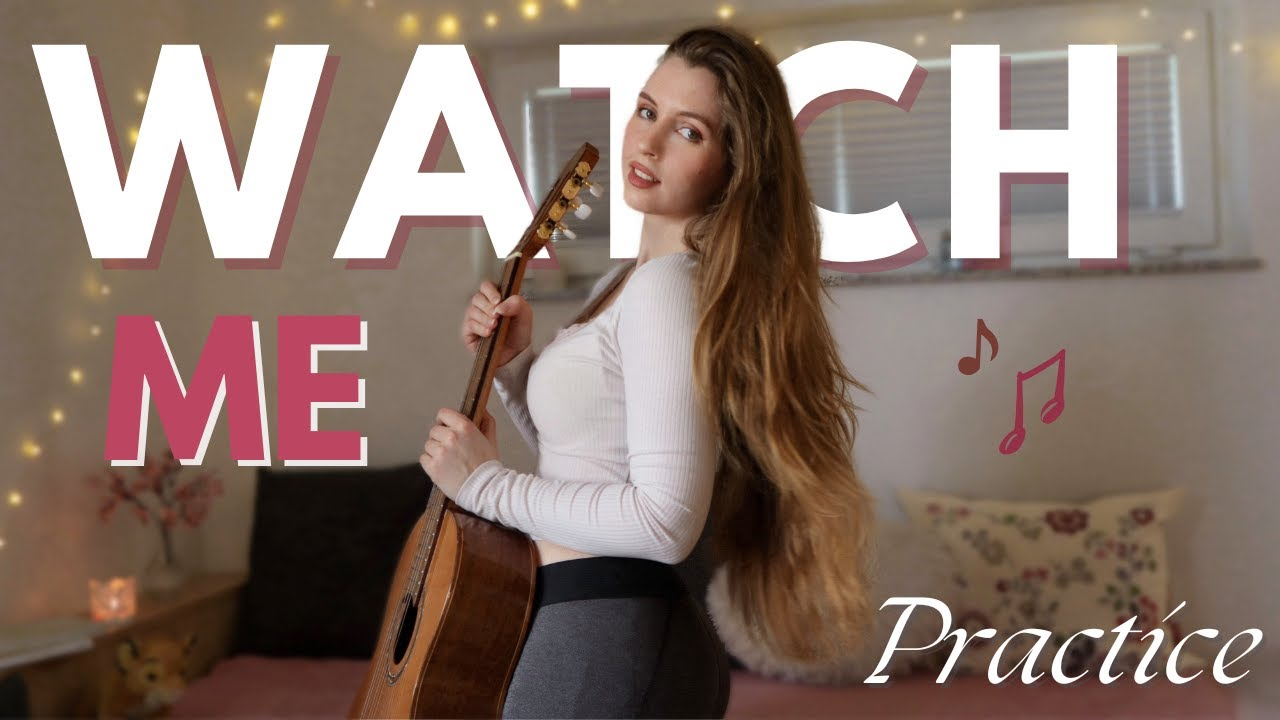
\includegraphics[width=0.48\linewidth]{pictures/youtube/2026/01/20260101_171831_youtube_001_XcQL_wZAdRA.jpg}
}
\end{center}

\subsection*{2026年01月03日 07:40}
\addcontentsline{toc}{subsection}{2026年01月03日 07:40}

2026年の正月（１月３日の朝）は雪模様です

小立野台地から犀川方向を臨むと、いつも街灯が見えていて気になっていました（おそらく御参詣坂と新桜坂の街灯なんだろうと推察しています）


(１)御参詣坂の街灯

御参詣坂（車は通行できません）を登ると平和町

自衛隊の基地や金沢大学附属の諸学校がある

奥には野田山（御参詣坂は野田山の墓参のための坂道だったとか）


(２)新桜坂の街灯

犀川にかかる桜橋から続く新桜坂（車が通れる道路です）

ここには、桜坂とW坂もあります

（この２つの坂の街灯は目立たないけどある様です）

この坂を登ると寺町

\paragraph{写真}
\begin{center}
\begin{minipage}{0.48\linewidth}
\centering
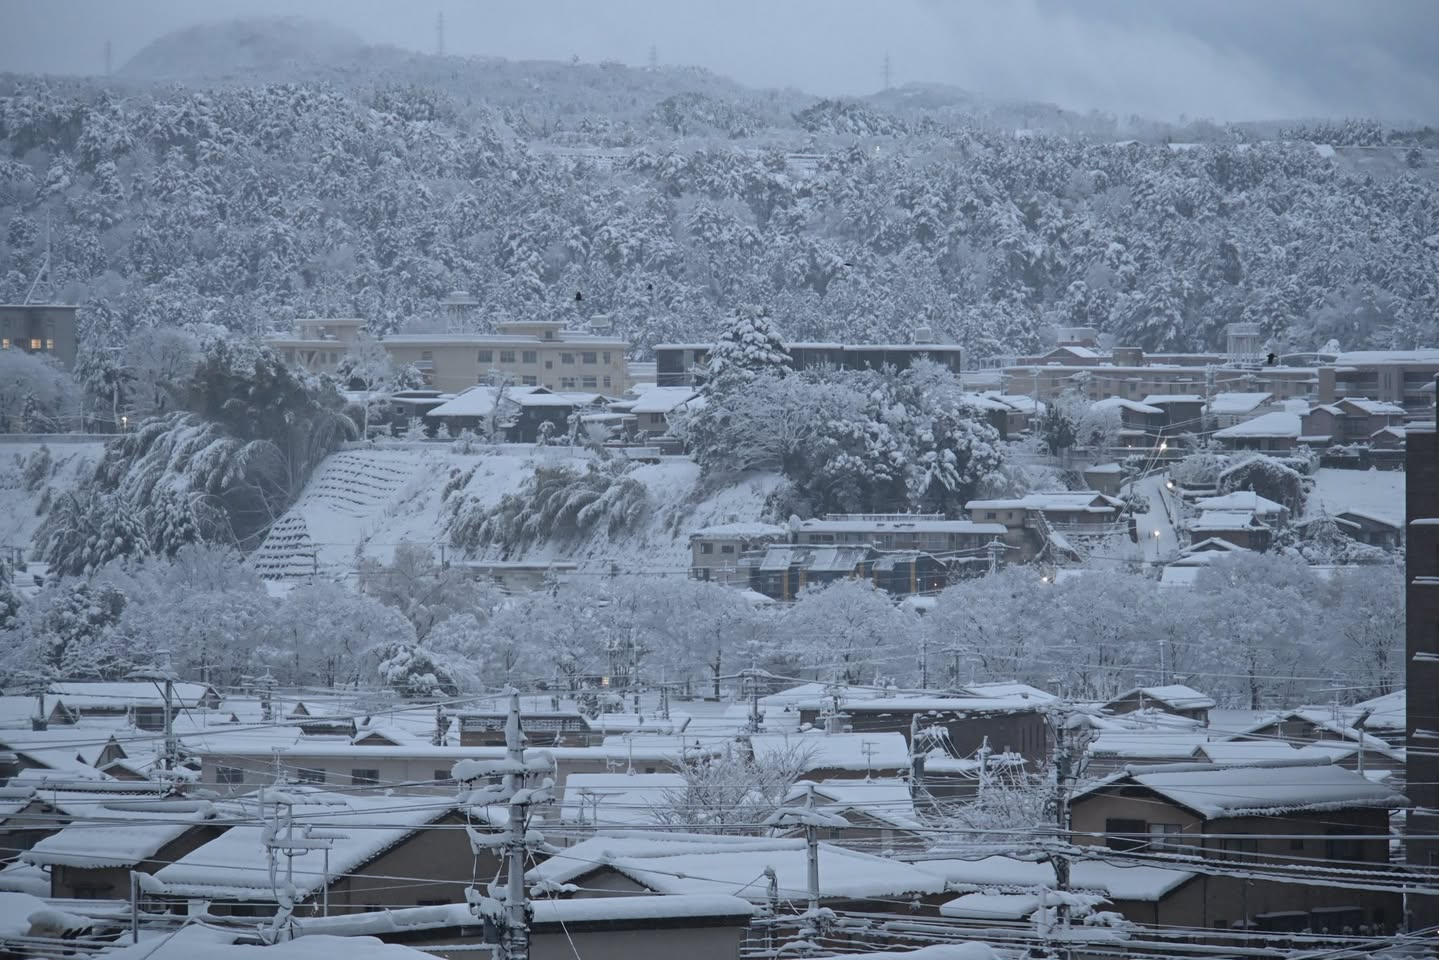
\includegraphics[width=\linewidth]{pictures/2026/01/20260103_074030_001.jpg}
\end{minipage}
\hfill
\begin{minipage}{0.48\linewidth}
\centering
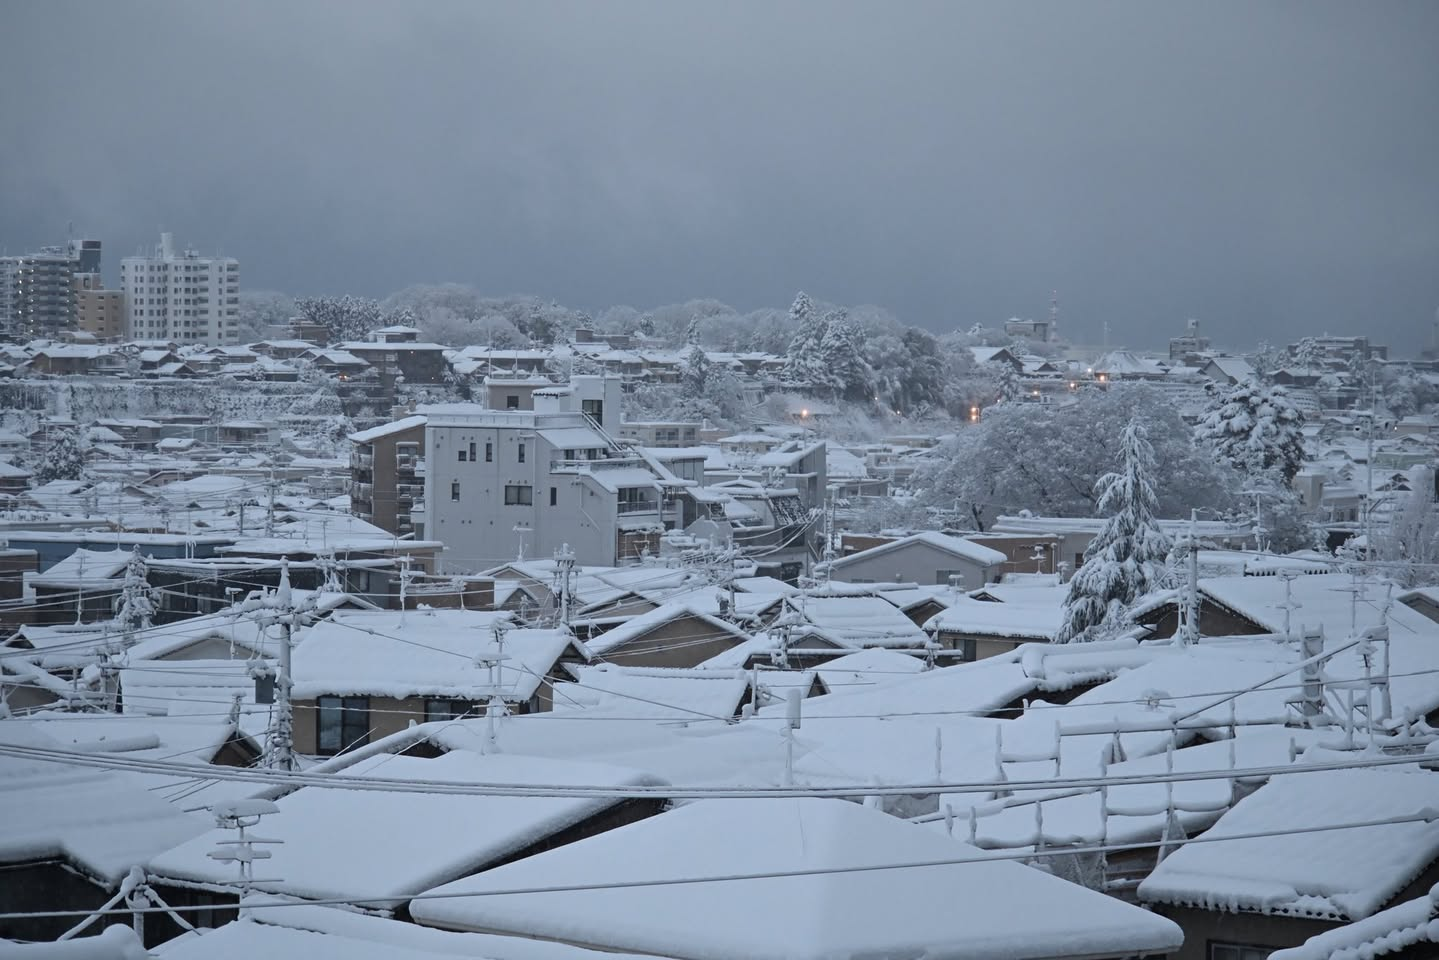
\includegraphics[width=\linewidth]{pictures/2026/01/20260103_074030_002.jpg}
\end{minipage}
\end{center}

\subsection*{2026年01月05日 17:51}
\addcontentsline{toc}{subsection}{2026年01月05日 17:51}

\paragraph{リンク}
\url{https://youtu.be/pLVv98VkWlk}

\begin{center}
\href{https://youtu.be/pLVv98VkWlk}{
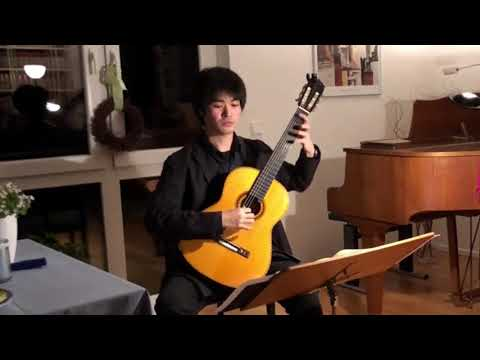
\includegraphics[width=0.48\linewidth]{pictures/youtube/2026/01/20260105_175106_youtube_001_pLVv98VkWlk.jpg}
}
\end{center}

\subsection*{2026年01月05日 17:51}
\addcontentsline{toc}{subsection}{2026年01月05日 17:51}

Lute曲以外、その他コラール等からの編曲

（お気に入りの曲を備忘のために整理した個人的LINK集）

=====


BWV147 主よ人の望みの喜びよ

\url{https://www.facebook.com/100002225117991/posts/9115943925156354/}




BWV156（BWV1056）シンフォニア

\url{https://m.facebook.com/story.php?story_fbid=24357756303881868&id=100002225117991}




BWV645（BWV140）目覚めよと呼ぶ声あり

\url{https://www.facebook.com/100002225117991/posts/24998283063162519/}




BWV816 フランス組曲 第５番 ト長調 アルマンド

\url{https://youtu.be/WVCbqRE0pZI}

\begin{center}
\href{https://youtu.be/WVCbqRE0pZI}{
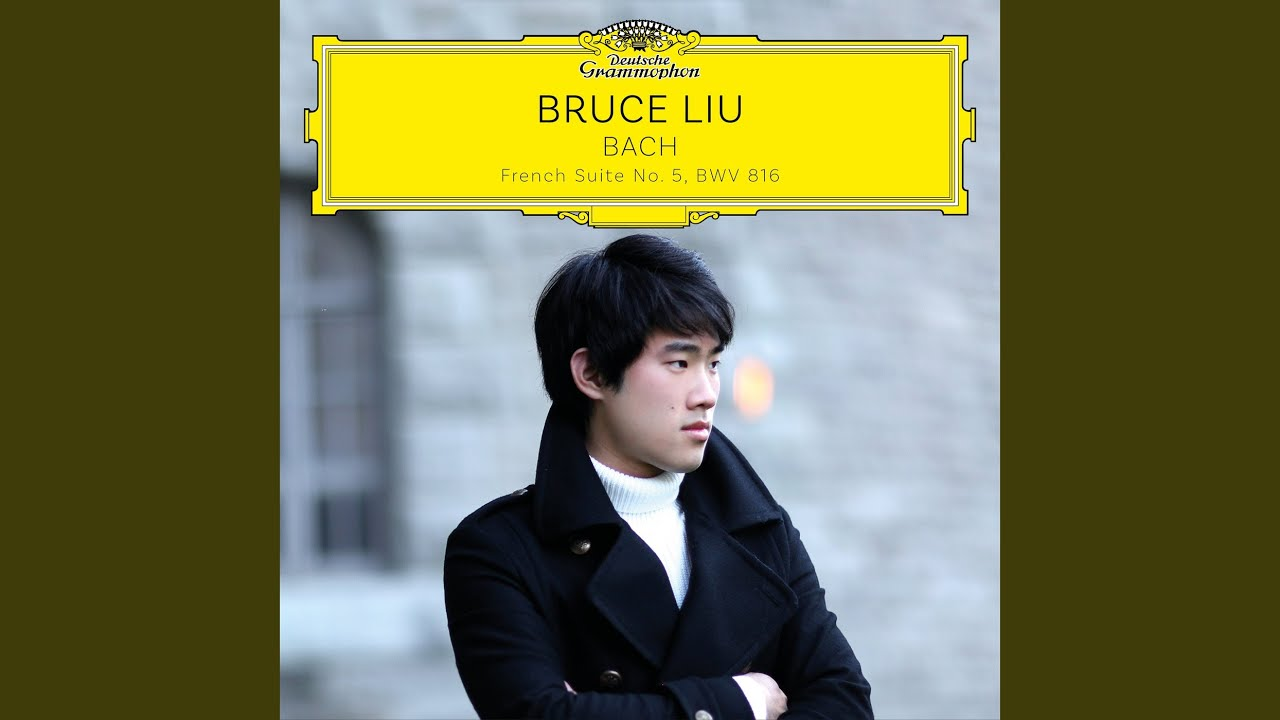
\includegraphics[width=0.48\linewidth]{pictures/youtube/2026/01/20260105_175132_youtube_001_WVCbqRE0pZI.jpg}
}
\end{center}



（どこかにギター編ないかな 二重奏ならある様だが）


BWV825 Partita

\url{https://www.facebook.com/100002225117991/posts/25577759395214880/}




BWV830 PartitaよりToccata

\url{https://youtu.be/KSSRijWjobE}

\begin{center}
\href{https://youtu.be/KSSRijWjobE}{
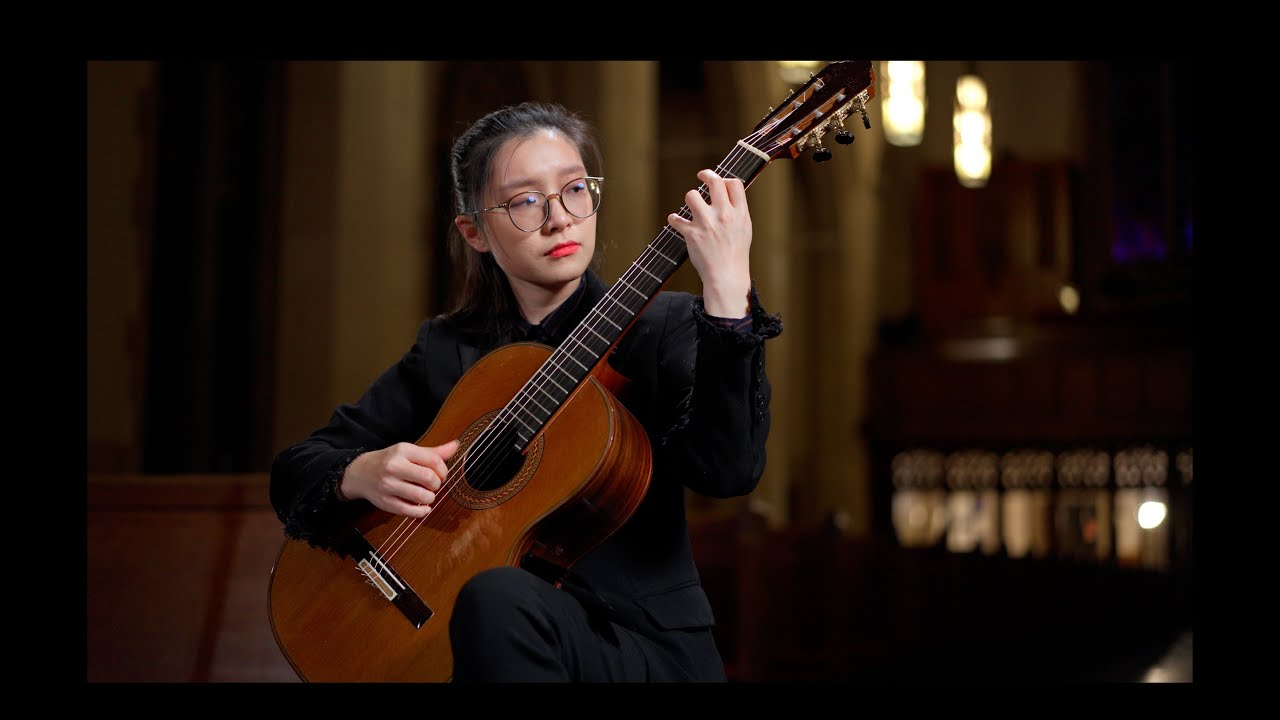
\includegraphics[width=0.48\linewidth]{pictures/youtube/2026/01/20260105_175132_youtube_002_KSSRijWjobE.jpg}
}
\end{center}




BWV846 平均律クラヴィア曲集No,1のPrelude

\url{https://www.facebook.com/100002225117991/posts/8961013527316062/}




BWV854 平均律クラヴィア曲集 No,9のPrelude

\url{https://www.facebook.com/100002225117991/posts/25129262530064571/}




BWV974（Adagio）

\url{https://youtu.be/89MPEr3hT-g}

\begin{center}
\href{https://youtu.be/89MPEr3hT-g}{
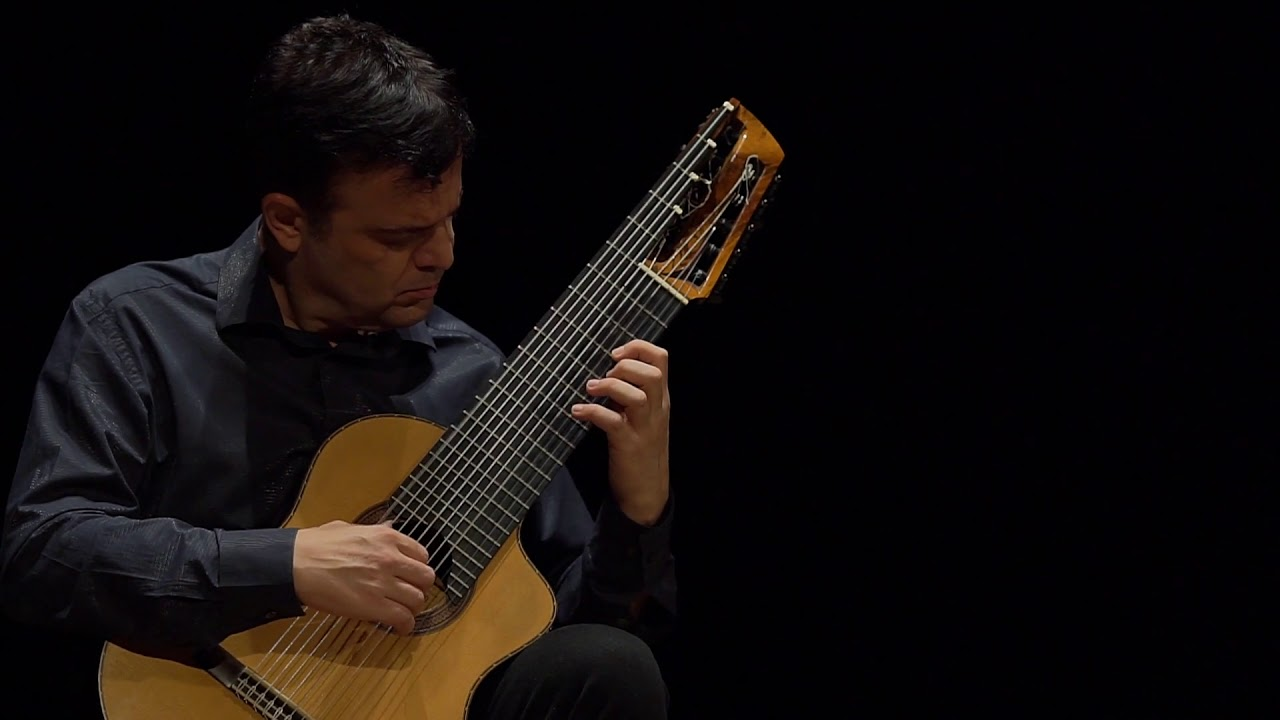
\includegraphics[width=0.48\linewidth]{pictures/youtube/2026/01/20260105_175132_youtube_003_89MPEr3hT-g.jpg}
}
\end{center}




BWV1068 管弦楽組曲より（G線上のアリア）

\url{https://www.facebook.com/100002225117991/posts/10074638062620264/}




=====

J.S.Bachのギター曲の全貌（？）はここ↓

\url{https://m.facebook.com/story.php?story_fbid=25468465252810962&id=100002225117991}




添付は↓日本に現存する最も古いオルガンだとの事

\url{https://www.taitogeibun.net/sougakudou/rekishi/pipe_organ/}



\paragraph{写真}
\begin{center}
\begin{minipage}{0.48\linewidth}
\centering
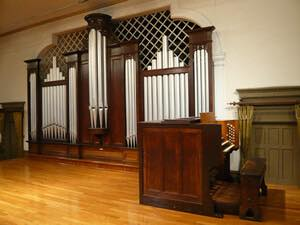
\includegraphics[width=\linewidth]{pictures/2026/01/20260105_175132_001.jpg}
\end{minipage}
\end{center}

\subsection*{2026年01月06日 11:28}
\addcontentsline{toc}{subsection}{2026年01月06日 11:28}

LuteSuiteなど、Luteのための曲

（お気に入りの曲を備忘のために整理した個人的LINK集）

=====


BWV995（3rdLuteSuite）

\url{https://youtu.be/FUnJBR5kR0I?t=137}

\begin{center}
\href{https://youtu.be/FUnJBR5kR0I?t=137}{
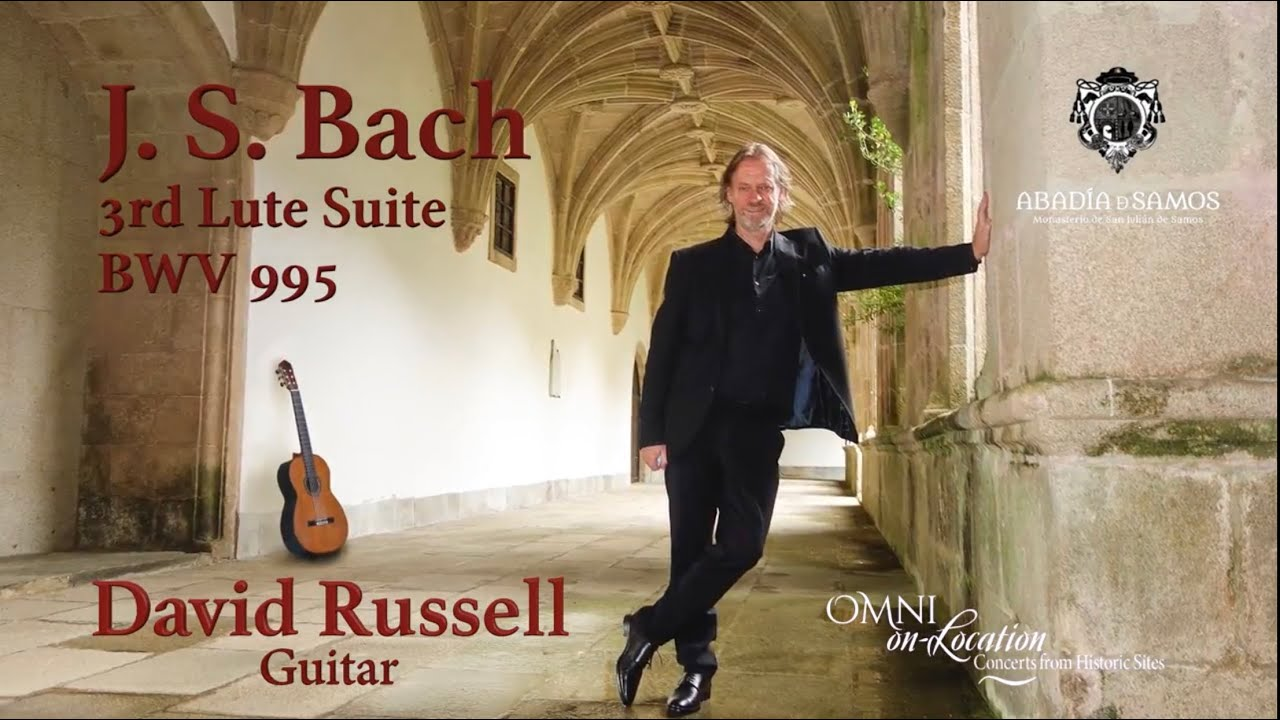
\includegraphics[width=0.48\linewidth]{pictures/youtube/2026/01/20260106_112804_youtube_001_FUnJBR5kR0I.jpg}
}
\end{center}




BWV996（1stLuteSuite）

\url{https://youtu.be/5fG6gDStP14?t=126}

\begin{center}
\href{https://youtu.be/5fG6gDStP14?t=126}{
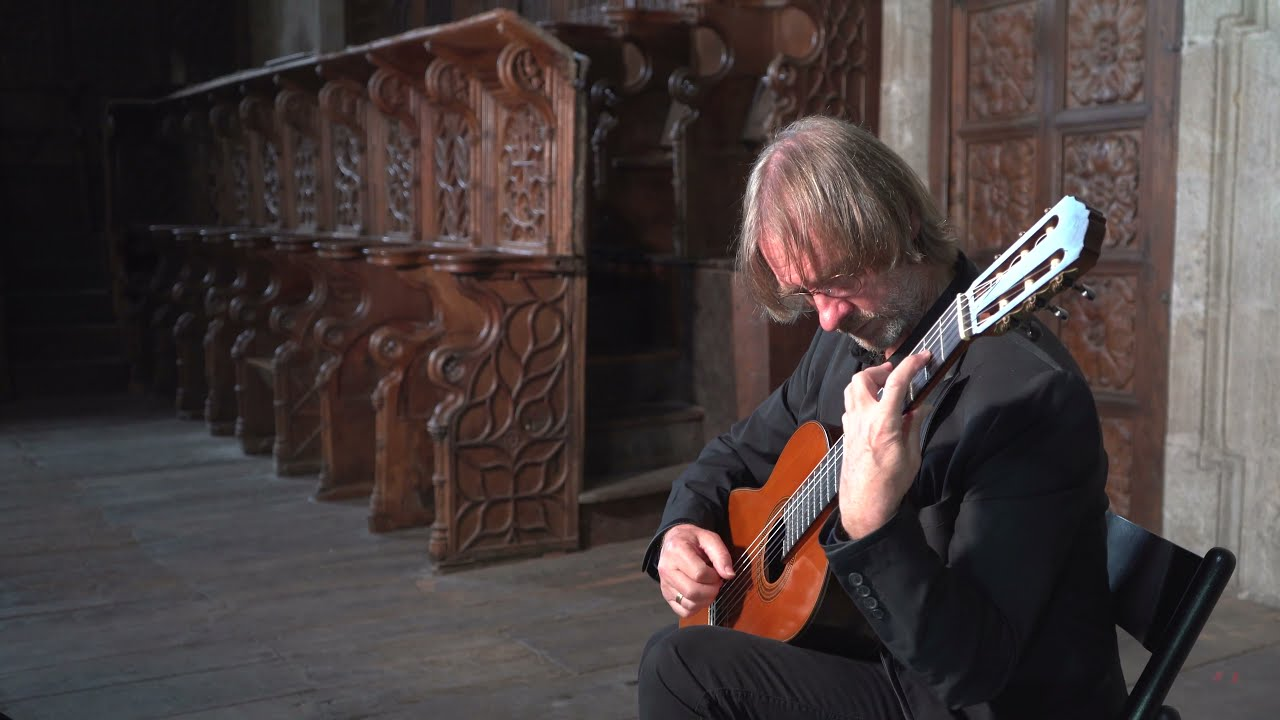
\includegraphics[width=0.48\linewidth]{pictures/youtube/2026/01/20260106_112804_youtube_002_5fG6gDStP14.jpg}
}
\end{center}




BWV997（2ndLuteSuite）

\url{https://youtu.be/NTB0EABbMw8?t=123}

\begin{center}
\href{https://youtu.be/NTB0EABbMw8?t=123}{
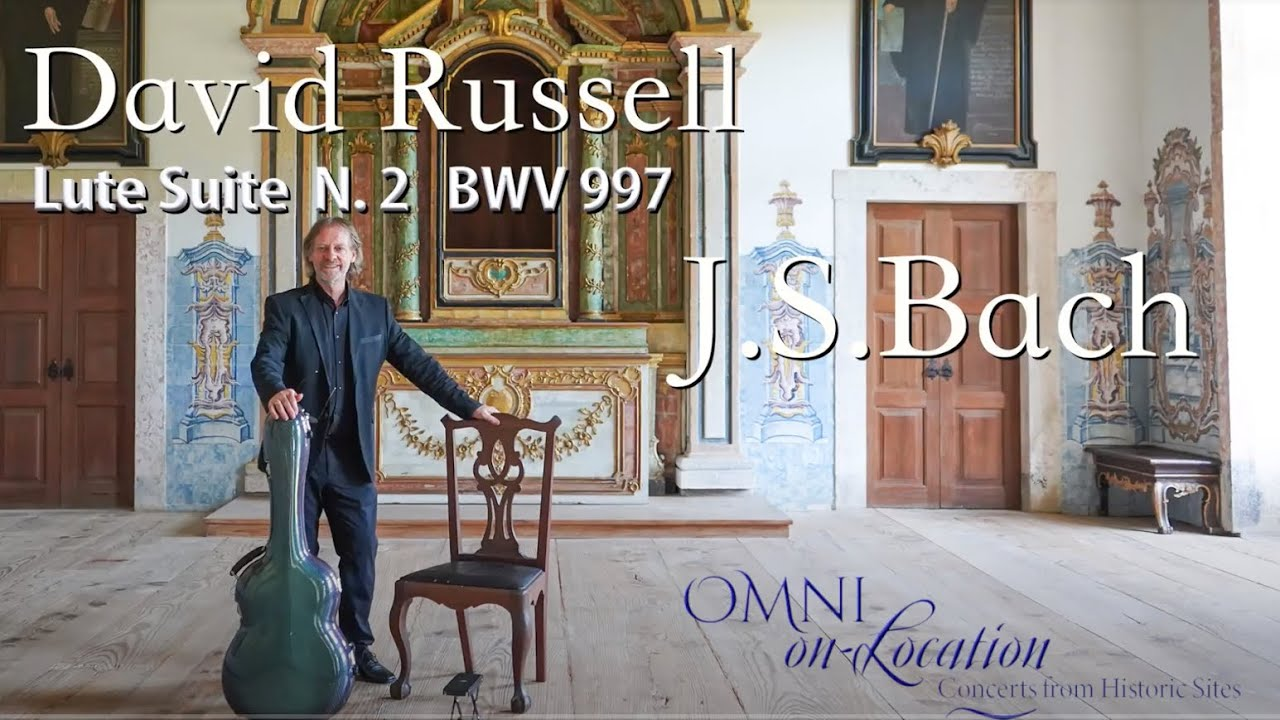
\includegraphics[width=0.48\linewidth]{pictures/youtube/2026/01/20260106_112804_youtube_003_NTB0EABbMw8.jpg}
}
\end{center}




BWV998（Prelude, Fugue and Allegro）

\url{https://www.facebook.com/100002225117991/posts/25408145472176274/}




BWV999（Prelude）

\url{https://www.facebook.com/100002225117991/posts/25390696953921126/}




BWV1000, 1001, 539

\url{https://www.facebook.com/100002225117991/posts/25129662370024587/}




BWV1006a（4thLuteSuite）

\url{https://youtu.be/DZh8rcIkNEY?t=100}

\begin{center}
\href{https://youtu.be/DZh8rcIkNEY?t=100}{
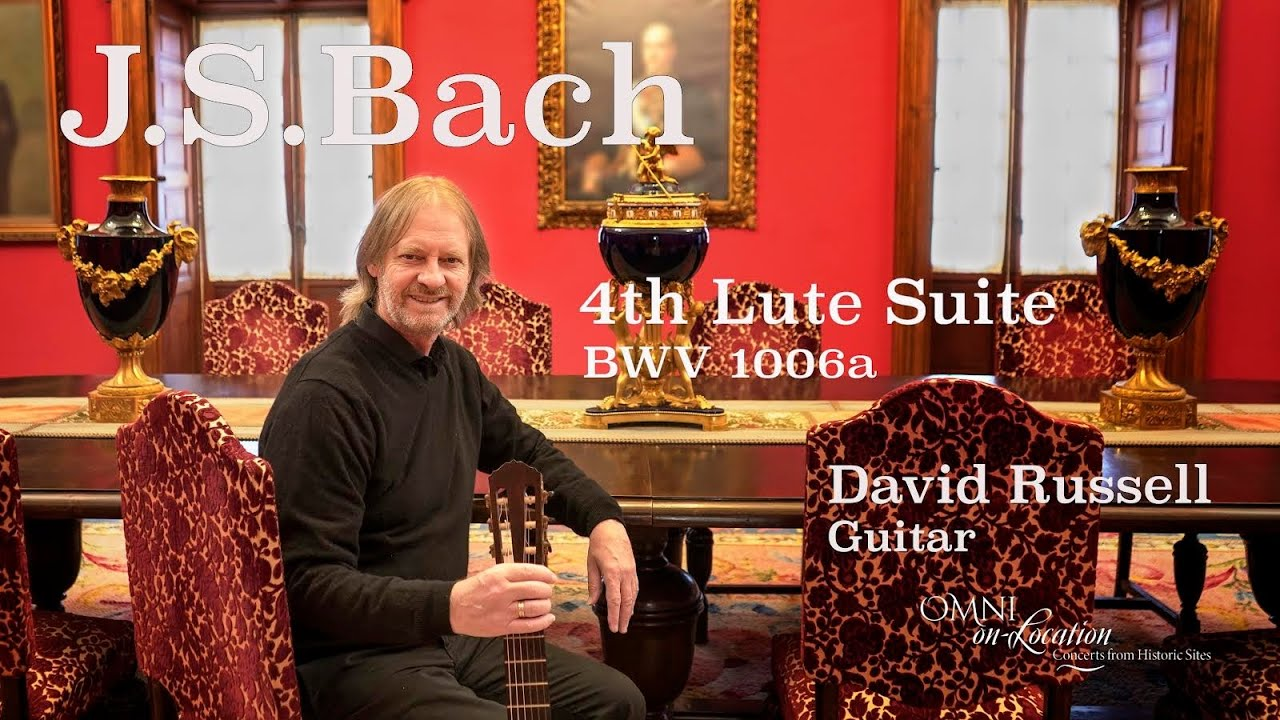
\includegraphics[width=0.48\linewidth]{pictures/youtube/2026/01/20260106_112804_youtube_004_DZh8rcIkNEY.jpg}
}
\end{center}




\url{https://m.facebook.com/groups/127443820942943/permalink/2835643086789656/}




=====

J.S.Bachのギター曲の全貌（？）はここ↓

\url{https://m.facebook.com/story.php?story_fbid=25468465252810962&id=100002225117991}



\paragraph{写真}
\begin{center}
\begin{minipage}{0.48\linewidth}
\centering
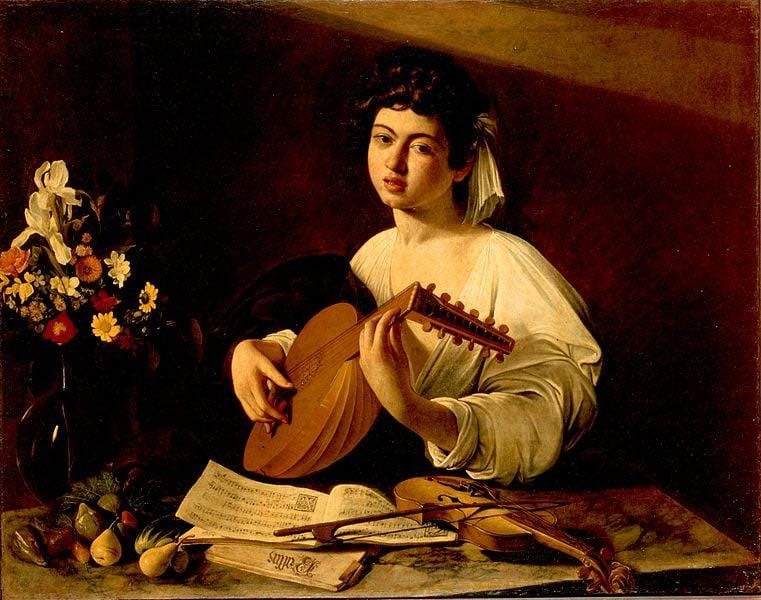
\includegraphics[width=\linewidth]{pictures/2026/01/20260106_112804_001.jpg}
\end{minipage}
\hfill
\begin{minipage}{0.48\linewidth}
\centering
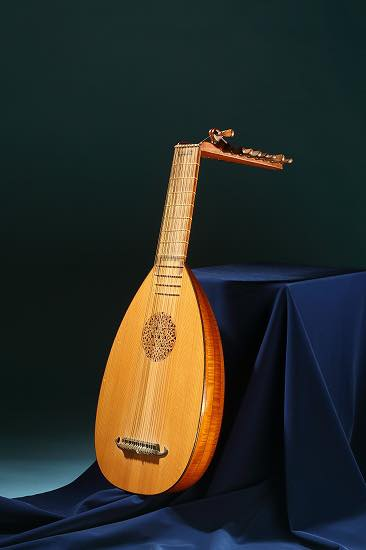
\includegraphics[width=\linewidth]{pictures/2026/01/20260106_112804_002.jpg}
\end{minipage}
\end{center}

\subsection*{2026年01月06日 17:42}
\addcontentsline{toc}{subsection}{2026年01月06日 17:42}

\url{https://www.facebook.com/photo.php?fbid=1339013598260559&set=a.471887998306461&type=3}




\url{https://www.facebook.com/photo.php?fbid=1293227919505794&set=a.471887998306461&type=3}



\subsection*{2026年01月07日 08:49}
\addcontentsline{toc}{subsection}{2026年01月07日 08:49}

BWV1001〜1006はViolinSonata and Partita

BWV1007〜1012はCelloSuites

\url{https://m.facebook.com/story.php?story_fbid=24232785103045656&id=100002225117991}



BWV1013はFlutePartita、BWV1034はFluteSonata


Cello組曲やViolinのソナタ、パルティータは、全曲ギター向けに編曲され演奏もされているが、以下ではその中から比較的ポピュラーなものを選んでみた（個人的Link集）

=====


BWV1002 Violin Partita No,1 より Sarabande

\url{https://www.facebook.com/100002225117991/posts/26074775385513276/}




BWV1004 Violin Partita No,2 よりChaconne

\url{https://www.facebook.com/100002225117991/posts/8370443646373056/}




BWV1005 ViolinSonata No,3よりLargo

\url{https://www.facebook.com/100002225117991/posts/24629723393351823/}




BWV1007 CelloSuite No,1 より Prelude

\url{https://m.facebook.com/story.php?story_fbid=24273505135640319&id=100002225117991}




BWV1012 CelloSuite No,6 より Prelude

\url{https://www.facebook.com/100002225117991/posts/26095048616819286/}




BWV1012 CelloSuite No,6 より Sarabande

\url{https://www.facebook.com/100002225117991/posts/24986489807675178/}




BWV1013 Flute Partita より

\url{https://www.facebook.com/100002225117991/posts/24319682991022533/}




BWV1034 FluteSonata より

\url{https://www.facebook.com/100002225117991/posts/24251950934462406/}




=====

J.S.Bachのギター曲の全貌（？）はここ↓

\url{https://m.facebook.com/story.php?story_fbid=25468465252810962&id=100002225117991}




添付↓は、バロック・ヴァイオリンとビオラ・ダ・ガンバ

\paragraph{写真}
\begin{center}
\begin{minipage}{0.48\linewidth}
\centering
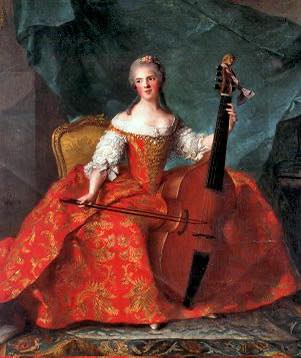
\includegraphics[width=\linewidth]{pictures/2026/01/20260107_084908_001.jpg}
\end{minipage}
\hfill
\begin{minipage}{0.48\linewidth}
\centering
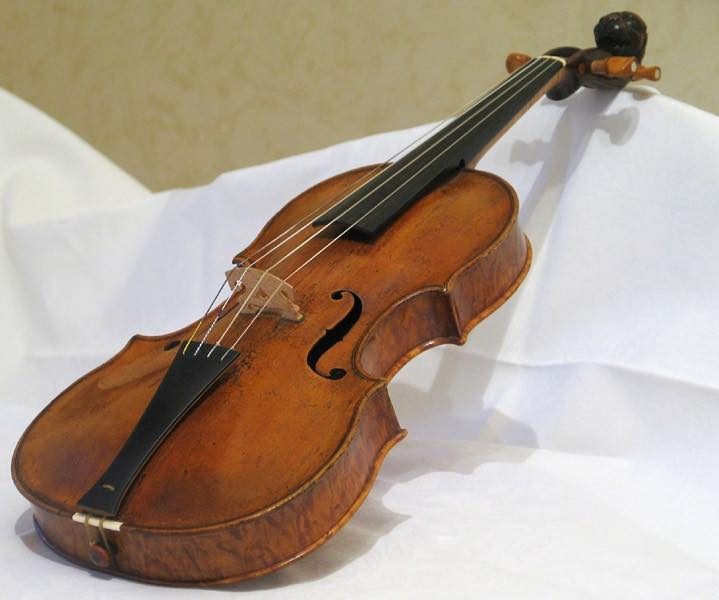
\includegraphics[width=\linewidth]{pictures/2026/01/20260107_084908_002.jpg}
\end{minipage}
\end{center}

\subsection*{2026年01月07日 08:54}
\addcontentsline{toc}{subsection}{2026年01月07日 08:54}

J.S.Bachのギター曲の全貌（？）

（お気に入りの曲を備忘のために整理した個人的LINK集です）


(１)LuteSuite他（Luteのための曲）

\url{https://www.facebook.com/100002225117991/posts/25460498406940980/}




(２)Violin Sonata, Partita、Cello Suite、Flute Sonata, Partita

\url{https://www.facebook.com/100002225117991/posts/25468437399480414/}




(3)Harpsichord Partita、その他コラールからの編曲等

\url{https://www.facebook.com/100002225117991/posts/25454278347562986/}




肖像画↓（1746年）

手に持っているのは6声のカノン （BWV1076）の楽譜だとか

\paragraph{写真}
\begin{center}
\begin{minipage}{0.48\linewidth}
\centering
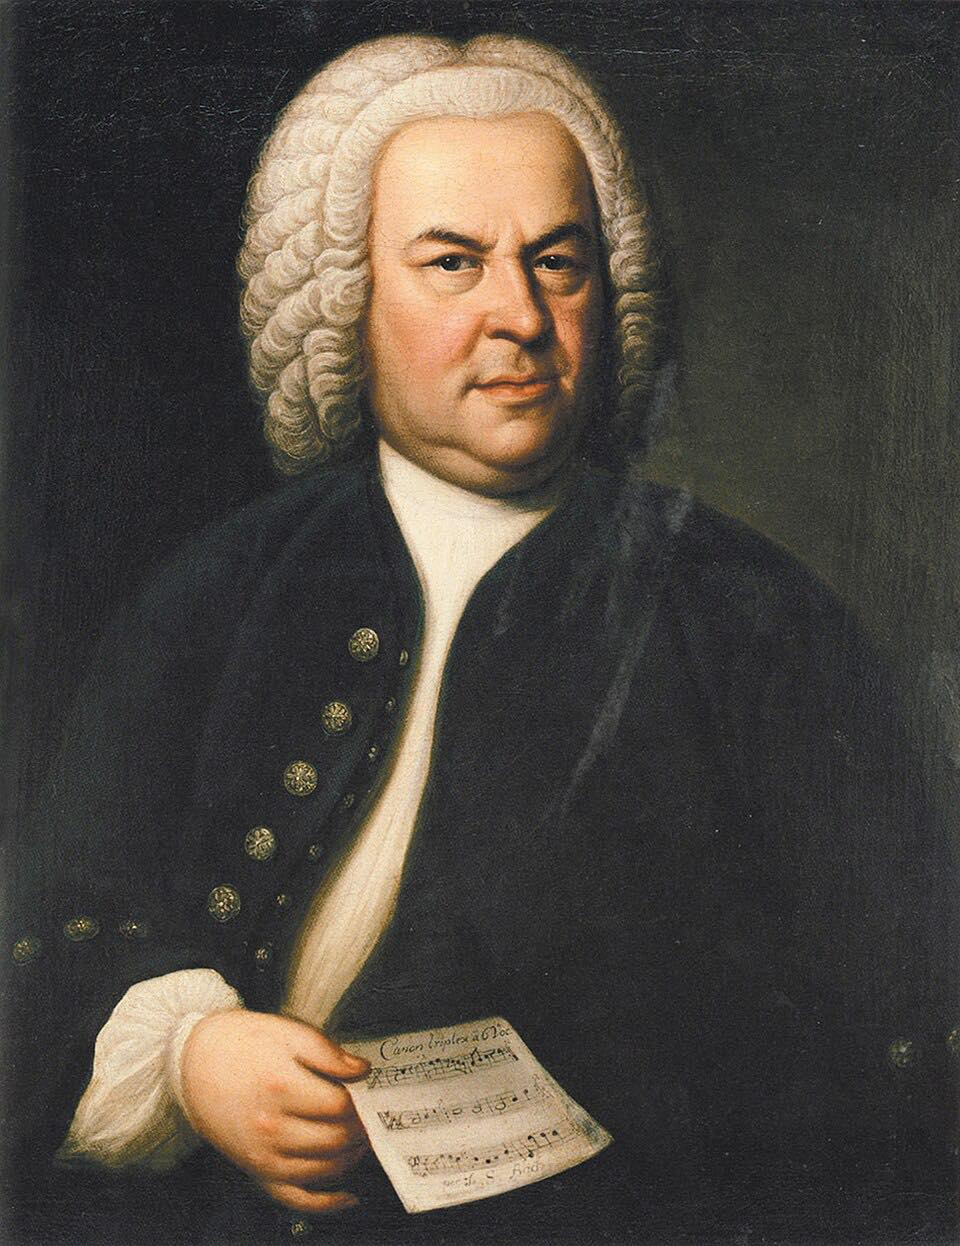
\includegraphics[width=\linewidth]{pictures/2026/01/20260107_085454_001.jpg}
\end{minipage}
\end{center}

\subsection*{2026年01月07日 22:22}
\addcontentsline{toc}{subsection}{2026年01月07日 22:22}

\paragraph{リンク}
\url{https://youtu.be/-zkPaGnKb5M}

\begin{center}
\href{https://youtu.be/-zkPaGnKb5M}{
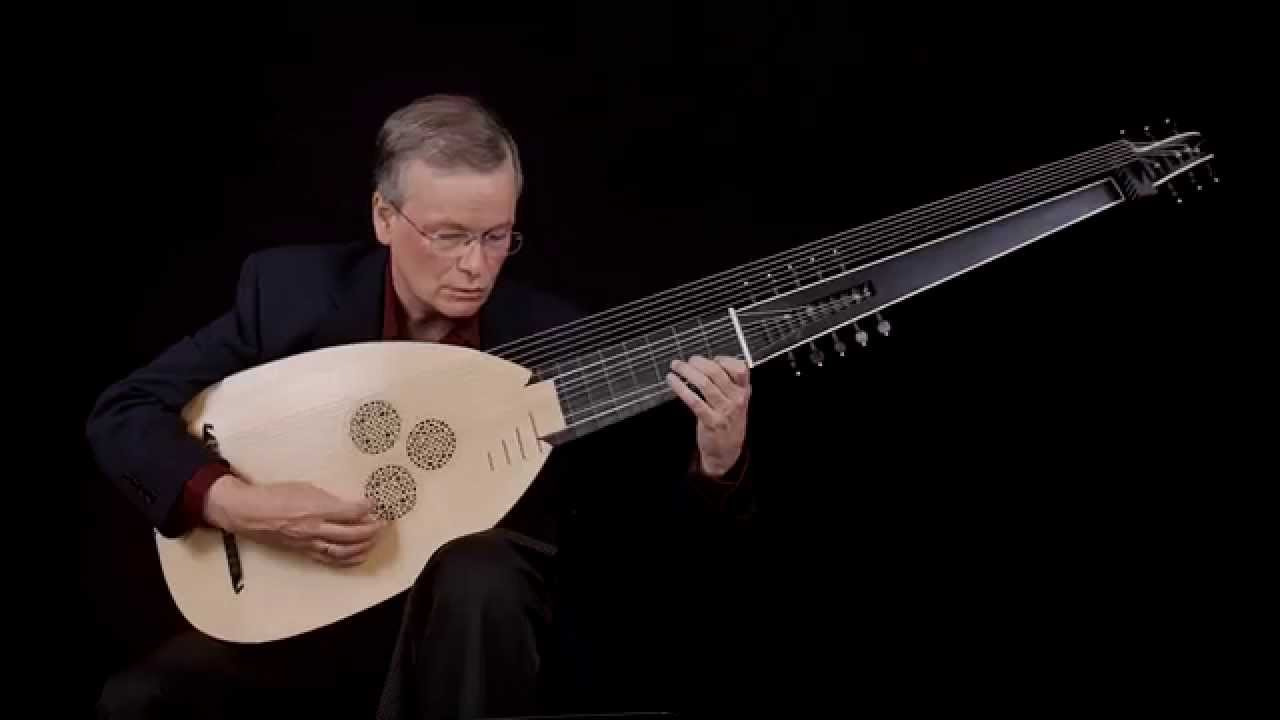
\includegraphics[width=0.48\linewidth]{pictures/youtube/2026/01/20260107_222215_youtube_001_-zkPaGnKb5M.jpg}
}
\end{center}

\subsection*{2026年01月09日 18:16}
\addcontentsline{toc}{subsection}{2026年01月09日 18:16}

\paragraph{リンク}
\url{https://youtu.be/BxOa2sBOZqk}

\begin{center}
\href{https://youtu.be/BxOa2sBOZqk}{
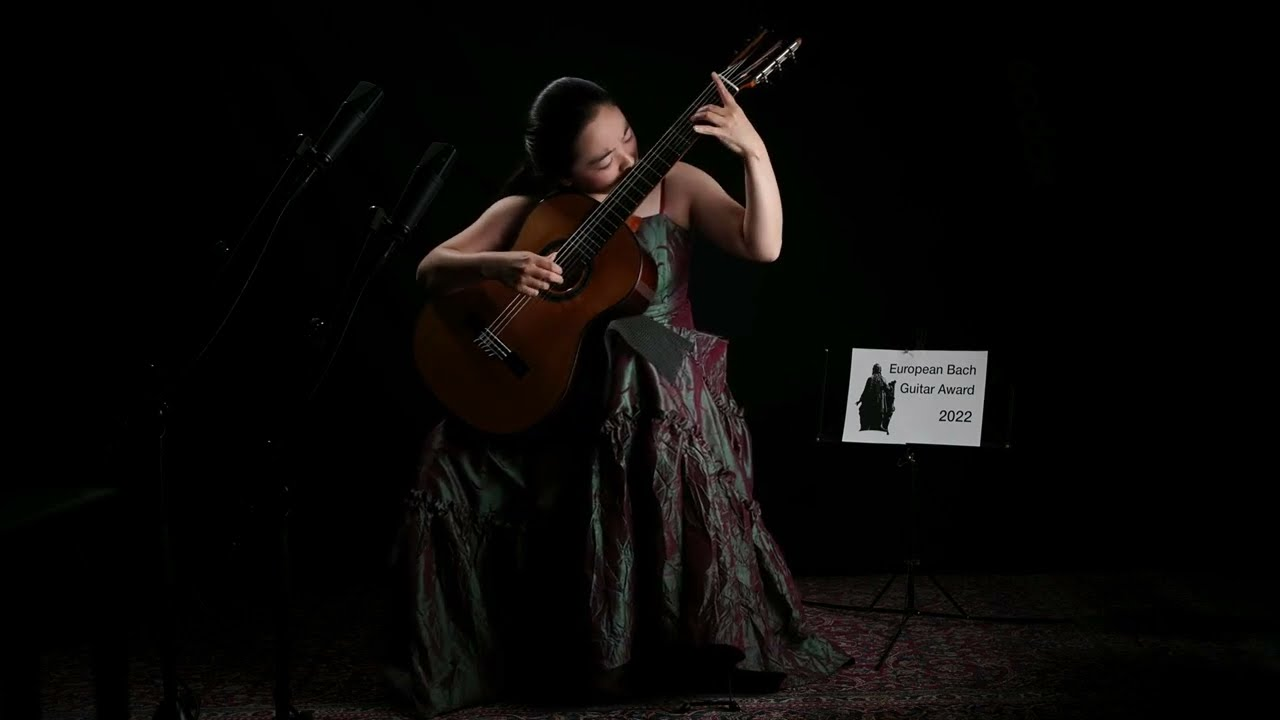
\includegraphics[width=0.48\linewidth]{pictures/youtube/2026/01/20260109_181623_youtube_001_BxOa2sBOZqk.jpg}
}
\end{center}

\subsection*{2026年01月10日 23:55}
\addcontentsline{toc}{subsection}{2026年01月10日 23:55}

\paragraph{リンク}
\url{https://youtu.be/uOuDzjCHeM4}

\begin{center}
\href{https://youtu.be/uOuDzjCHeM4}{
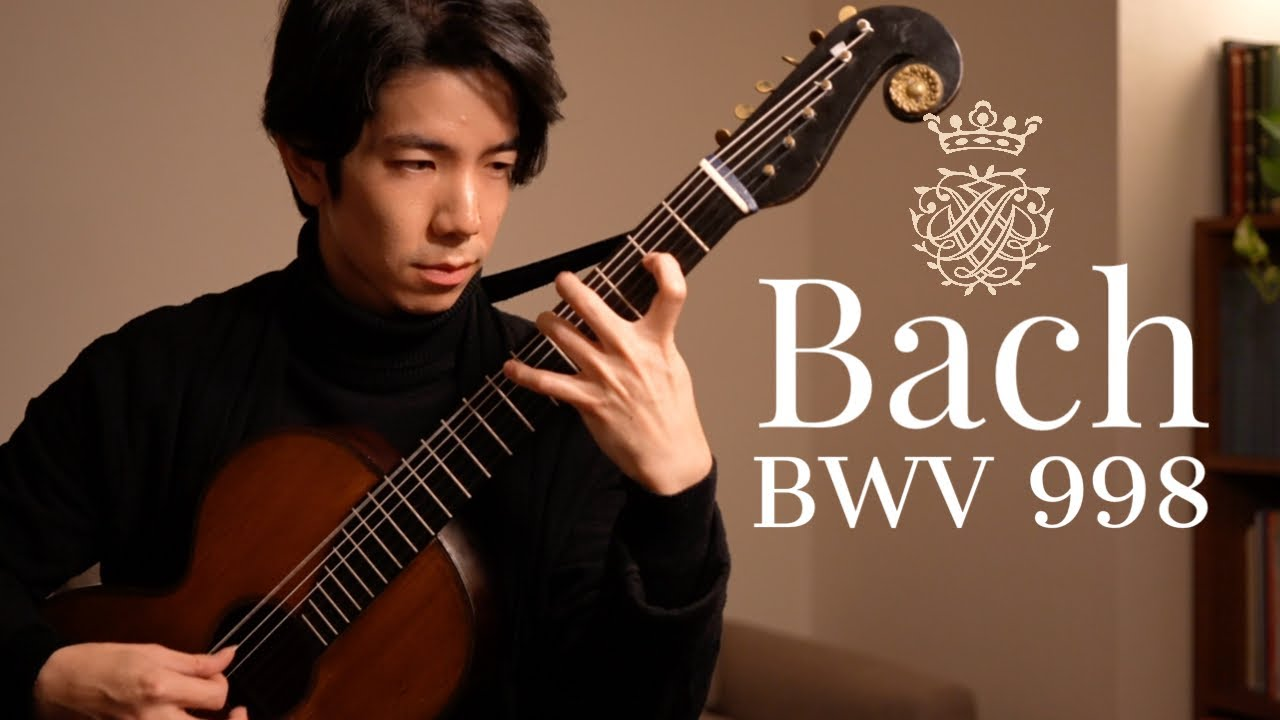
\includegraphics[width=0.48\linewidth]{pictures/youtube/2026/01/20260110_235510_youtube_001_uOuDzjCHeM4.jpg}
}
\end{center}

\subsection*{2026年01月11日 09:33}
\addcontentsline{toc}{subsection}{2026年01月11日 09:33}

Bach三昧！全6曲中4曲がBachだ

（こんなに沢山のBachを演奏するものなのか）

前半では、他の曲（タンスマン←私の知らない曲）を間に挟んでBachのLute組曲を2曲

後半はPrelude, FugueとAllegroで始まり、バリオスの大聖堂を挟んでやはりBachを2曲（大聖堂が息抜きになっている？）

（後ろの方に行くほど気持ちが高ぶる様に曲が仕組まれているのか）

そして最後は、大曲Chaconneでしめようという意図かと、、

（しかもBachはどれも山下氏自身によるこだわりの編曲か）


楽しみなプログラムだな〜、きっと幸せな時間を過ごせそうです

是非BachのCDを出してほしいものです（期待してます）

ちょっと遠いんだけど、聞きに行きたくなってきました

（でも、桜の季節の京都はcrowdedで、ホテルはexpensiveになるんだろうな）


チケットは↓ここ

\url{https://m.facebook.com/story.php?story_fbid=1468618141930778&id=100063478182933}



\paragraph{写真}
\begin{center}
\begin{minipage}{0.48\linewidth}
\centering
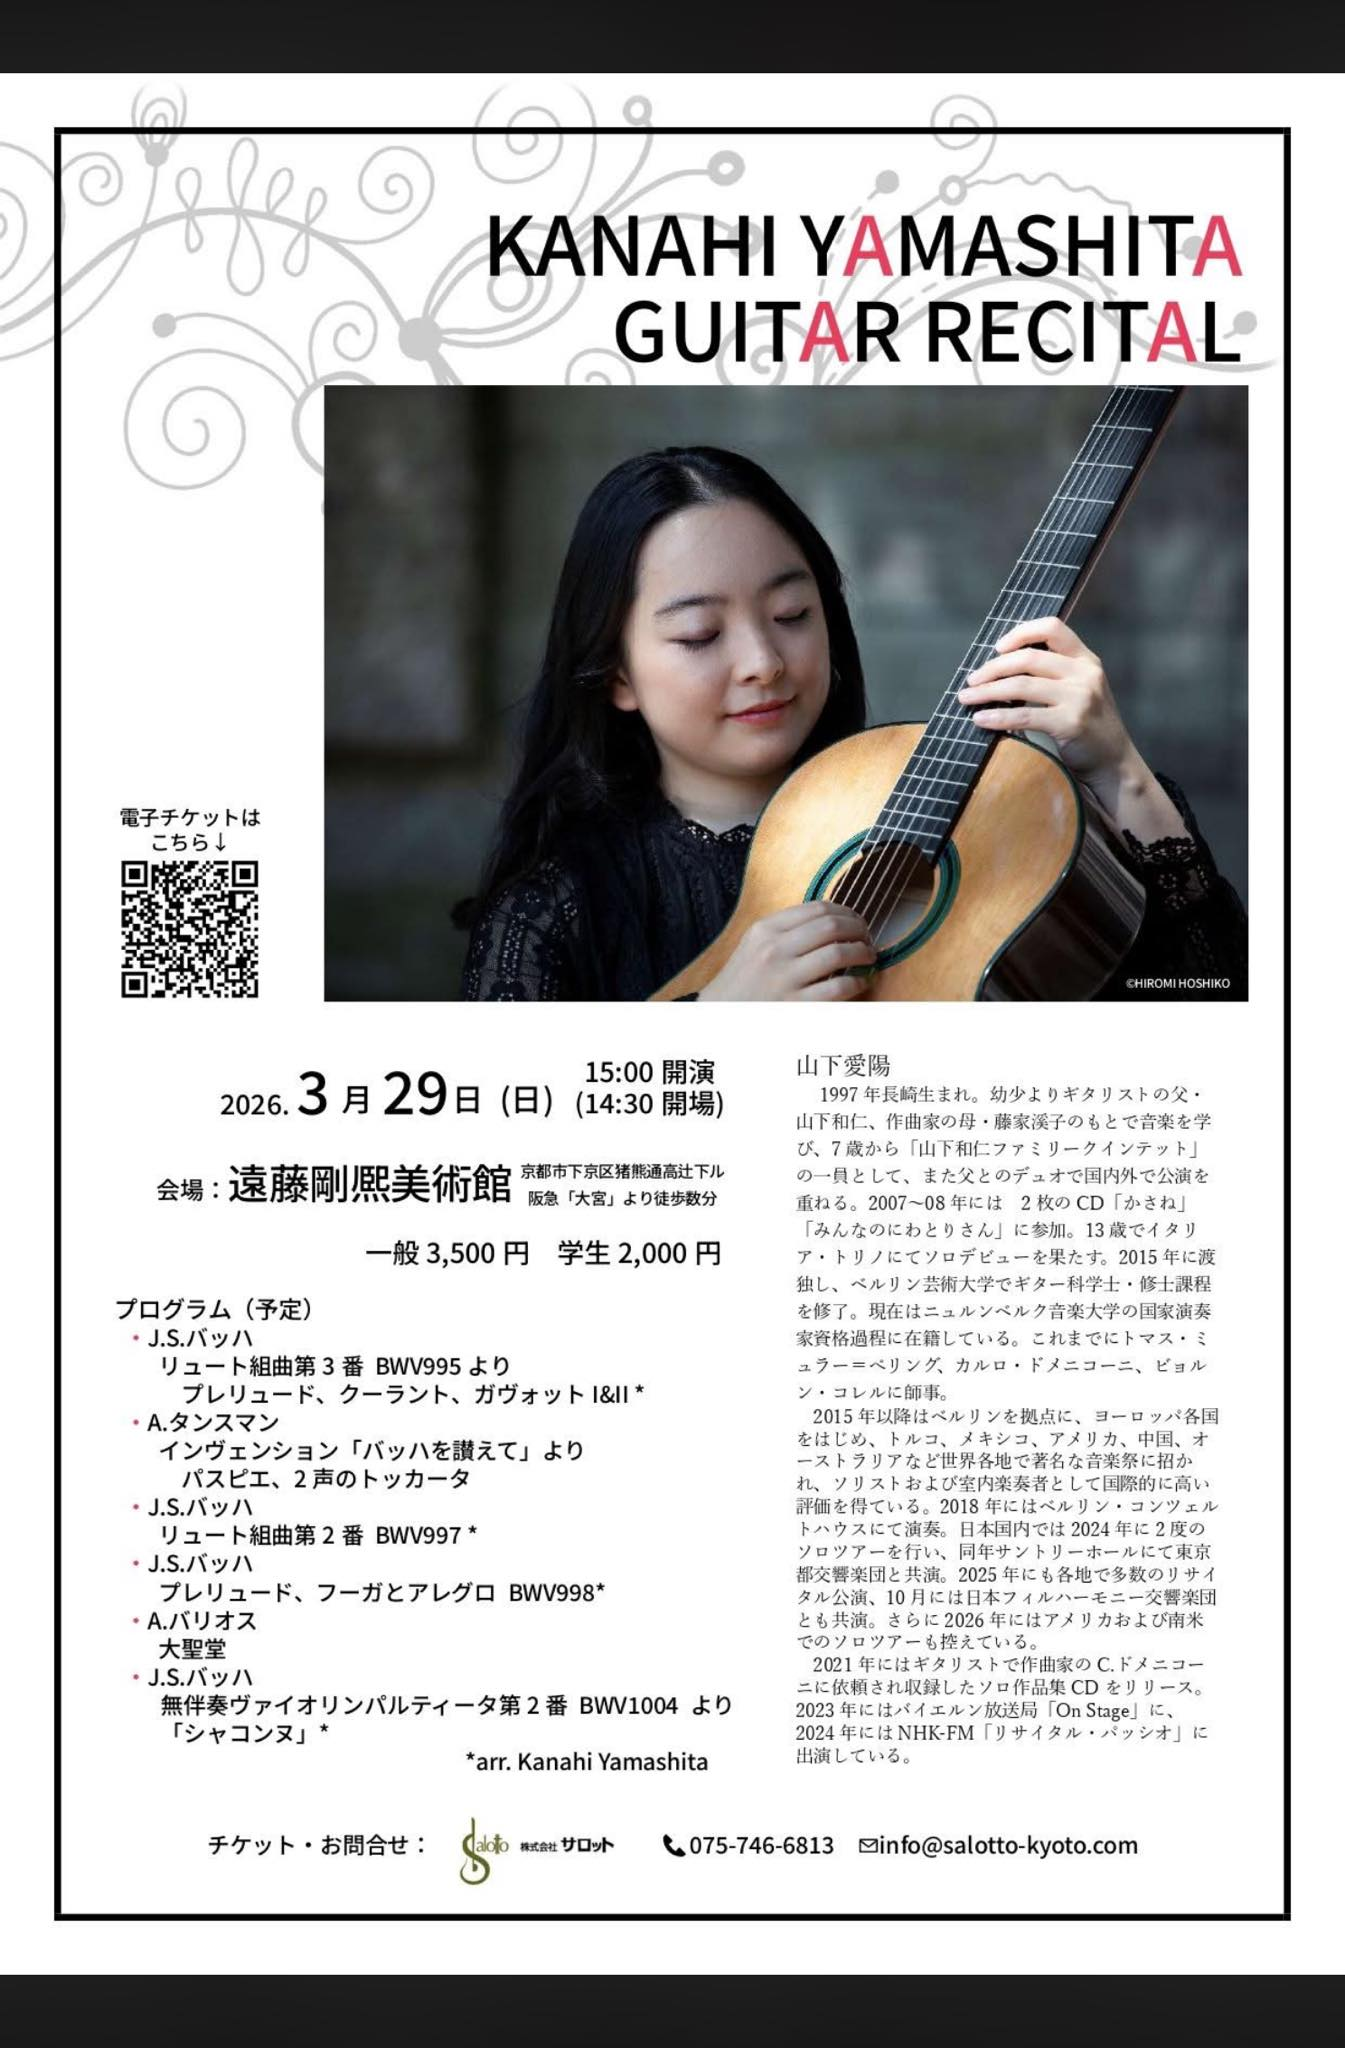
\includegraphics[width=\linewidth]{pictures/2026/01/20260111_093324_001.jpg}
\end{minipage}
\end{center}

\subsection*{2026年01月11日 11:06}
\addcontentsline{toc}{subsection}{2026年01月11日 11:06}

\paragraph{リンク}
\url{https://youtu.be/d1_b_Isdelw}

\begin{center}
\href{https://youtu.be/d1_b_Isdelw}{
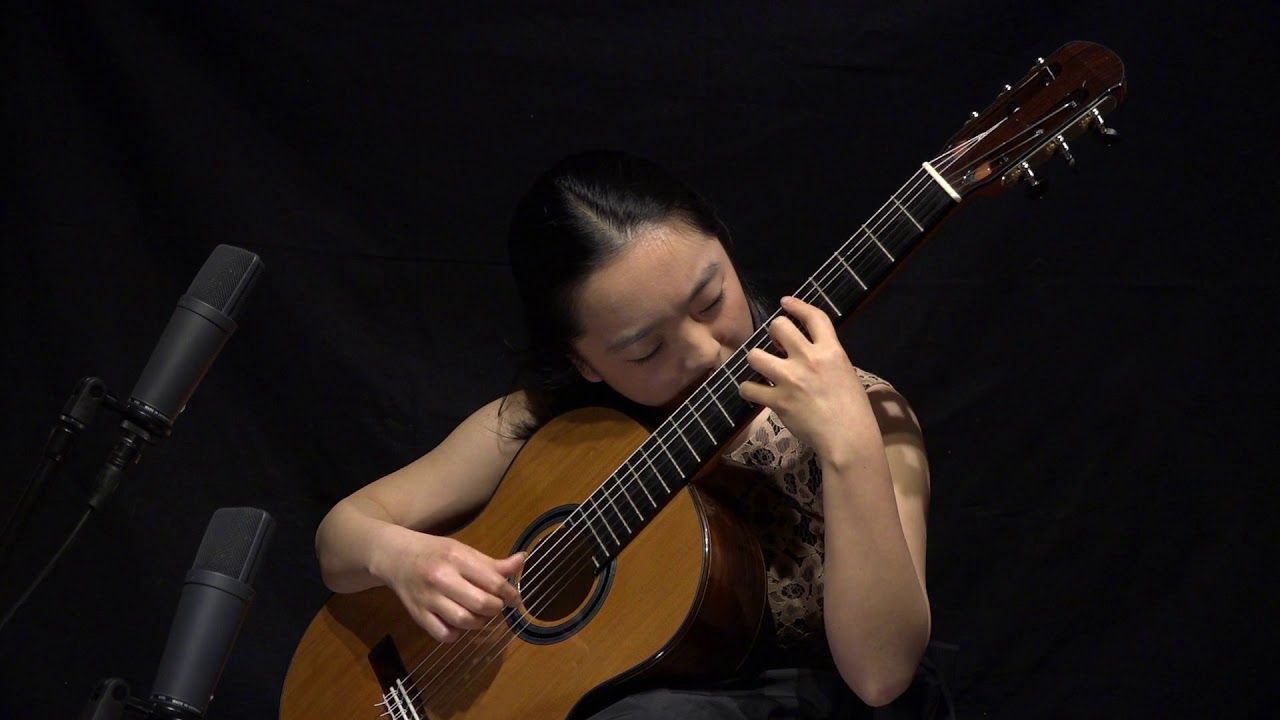
\includegraphics[width=0.48\linewidth]{pictures/youtube/2026/01/20260111_110648_youtube_001_d1_b_Isdelw.jpg}
}
\end{center}

\subsection*{2026年01月11日 11:07}
\addcontentsline{toc}{subsection}{2026年01月11日 11:07}

\paragraph{リンク}
\url{https://youtu.be/xljWbyxOaH8}

\begin{center}
\href{https://youtu.be/xljWbyxOaH8}{
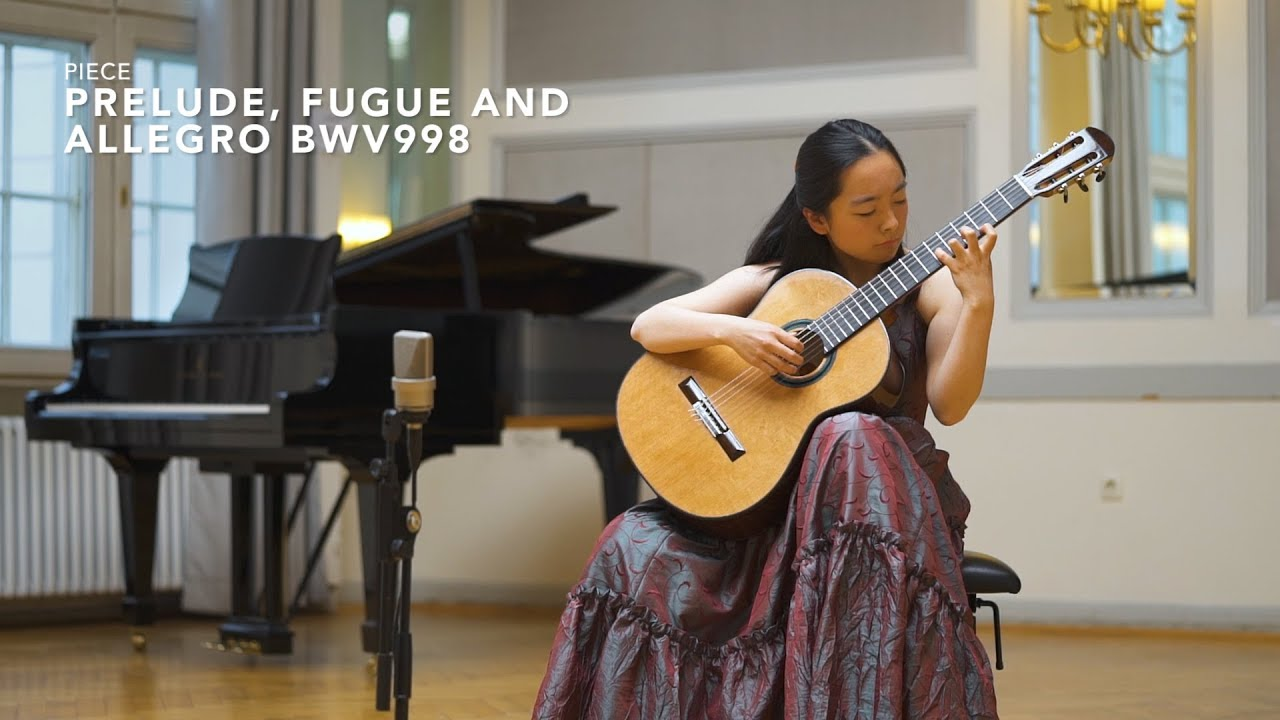
\includegraphics[width=0.48\linewidth]{pictures/youtube/2026/01/20260111_110737_youtube_001_xljWbyxOaH8.jpg}
}
\end{center}

\subsection*{2026年01月12日 00:14}
\addcontentsline{toc}{subsection}{2026年01月12日 00:14}

\paragraph{リンク}
\url{https://youtu.be/zMiOPtTEpZU}

\begin{center}
\href{https://youtu.be/zMiOPtTEpZU}{
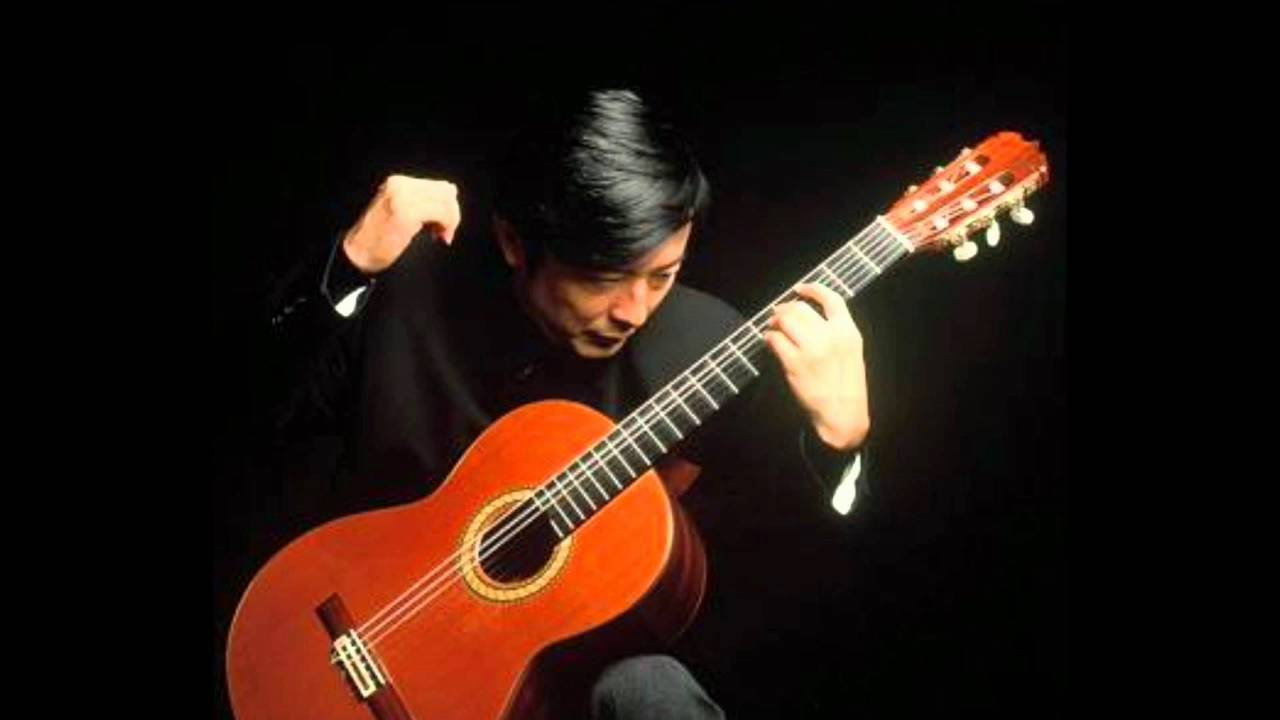
\includegraphics[width=0.48\linewidth]{pictures/youtube/2026/01/20260112_001414_youtube_001_zMiOPtTEpZU.jpg}
}
\end{center}

\subsection*{2026年01月15日 11:57}
\addcontentsline{toc}{subsection}{2026年01月15日 11:57}

兼六園に梅の花咲いてるよとニュースで言っていたので行ってみた。まだ1月15日ですけど、こんなに早い時期に咲くものなんですね。


私と同様、カメラで狙っている人は思いの外たくさん見かけた。でも未だチラホラで、高い所の枝を真剣に探さないと開いている花はなかなか見つからないし、高いところ（遠く）で咲いていても、その花は写真（絵）にならない。昔、国語の先生に聞いた話によると、万葉集では概して「梅は近景、桜は遠景」で歌われているのだとか。写真も同じ様な気がします。梅は近づいて撮らなくちゃ、なかなか絵になりません。


札には八重寒紅と書かれていたかな。目の前に咲いていた（希少で貴重な）花を撮影していた時に、ふと後ろの人気（ひとけ）に振り向くと、iPhoneやカメラを構えた人が列を作って順番を待っていらしたのでびっくり。取り急ぎ、あたふたと退散しました。

\paragraph{写真}
\begin{center}
\begin{minipage}{0.48\linewidth}
\centering
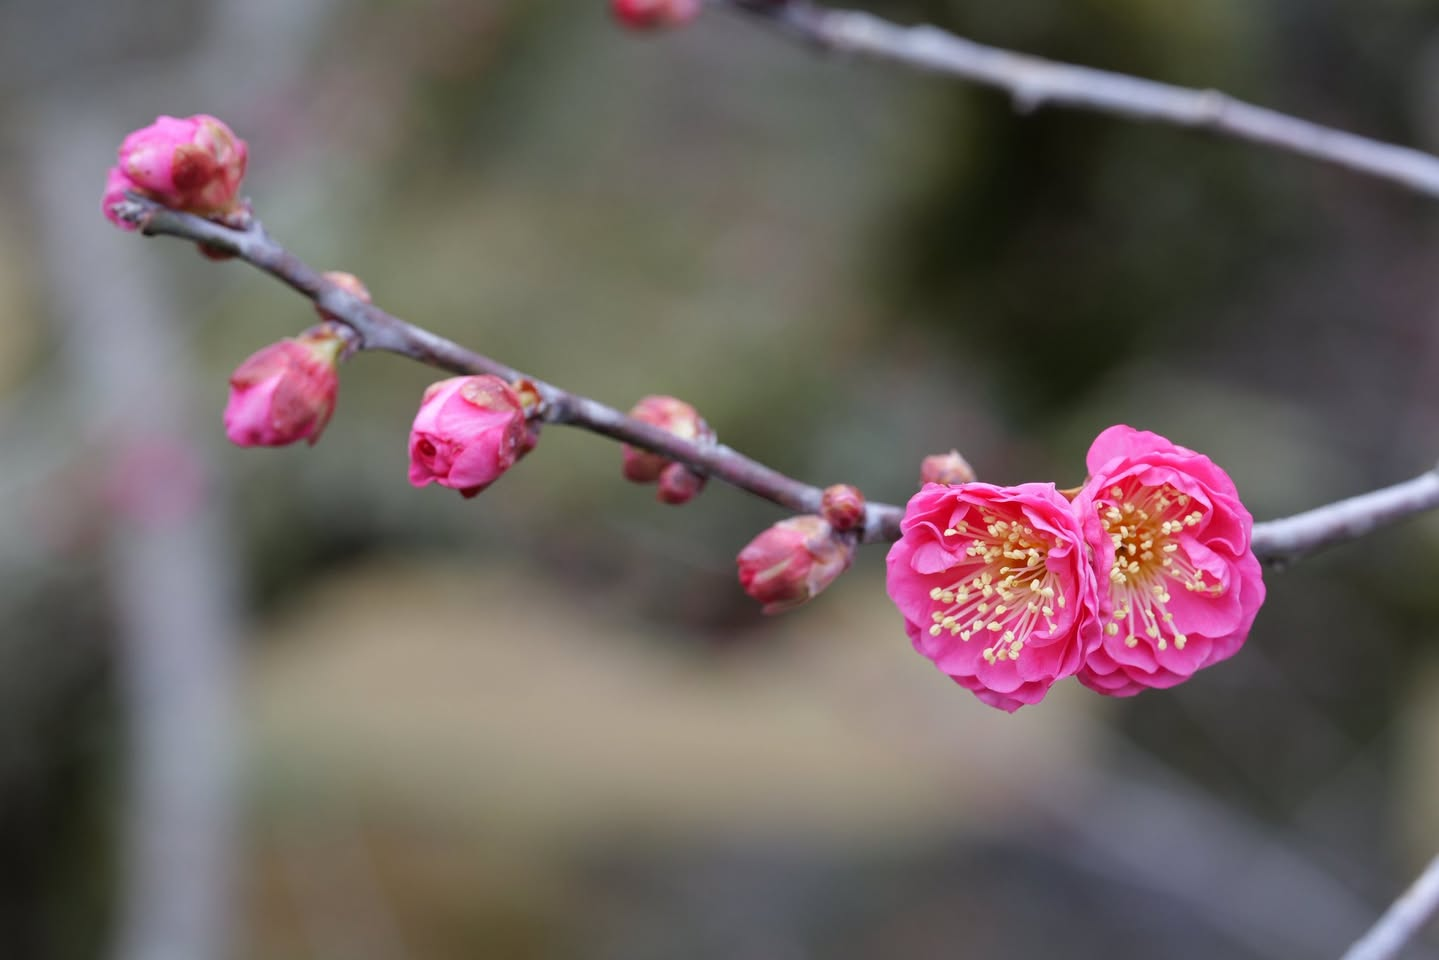
\includegraphics[width=\linewidth]{pictures/2026/01/20260115_115754_001.jpg}
\end{minipage}
\hfill
\begin{minipage}{0.48\linewidth}
\centering
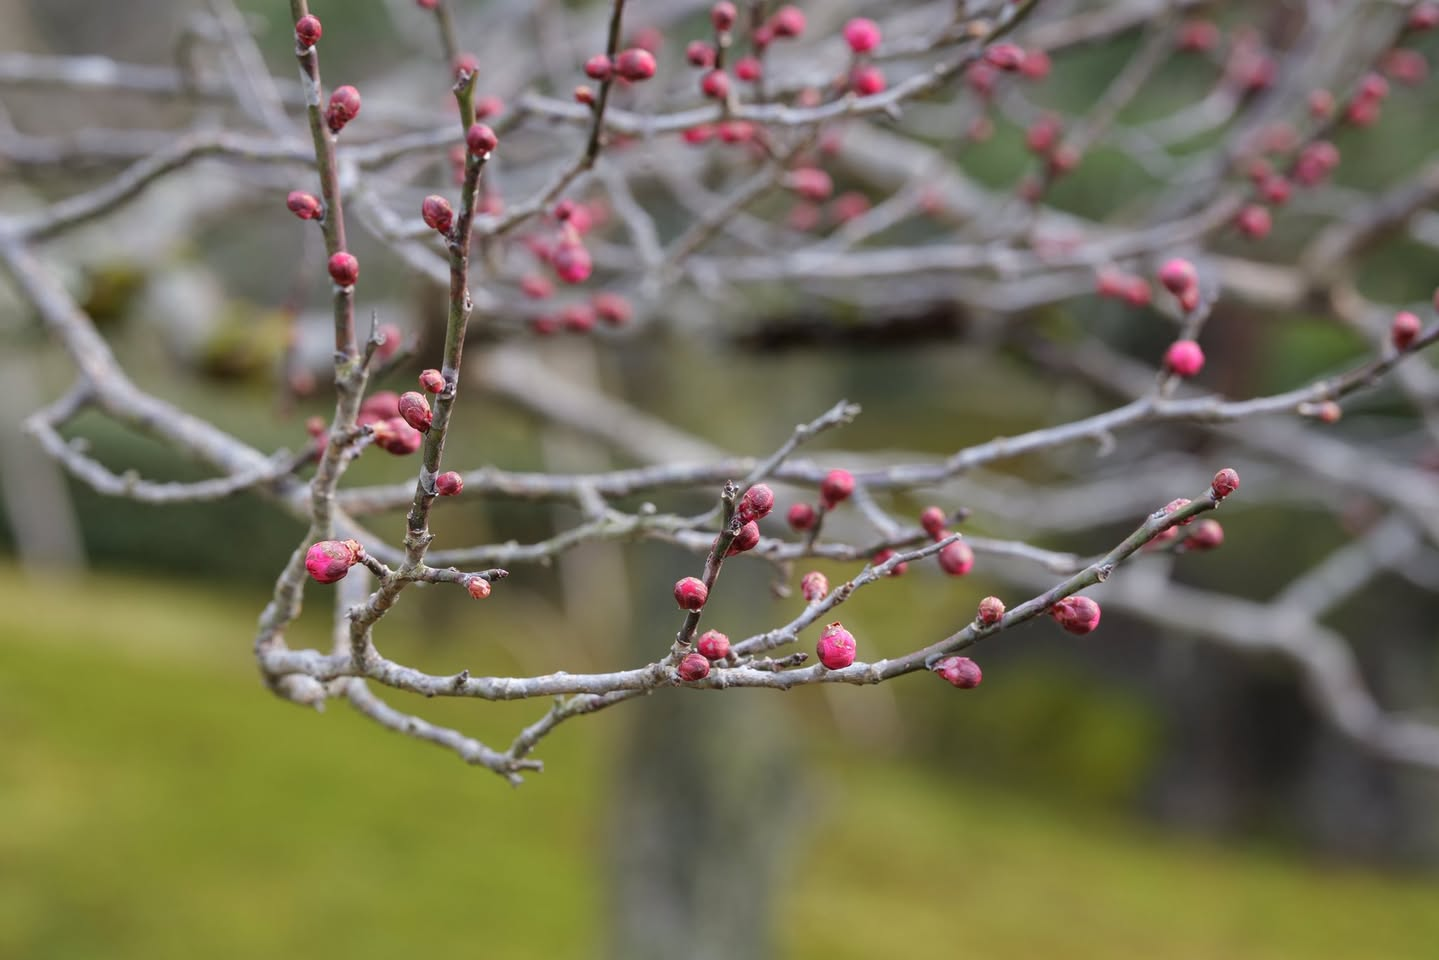
\includegraphics[width=\linewidth]{pictures/2026/01/20260115_115754_002.jpg}
\end{minipage}
\end{center}

\subsection*{2026年01月15日 21:29}
\addcontentsline{toc}{subsection}{2026年01月15日 21:29}

\paragraph{リンク}
\url{https://youtu.be/mIOtV8KUQHE}

\begin{center}
\href{https://youtu.be/mIOtV8KUQHE}{
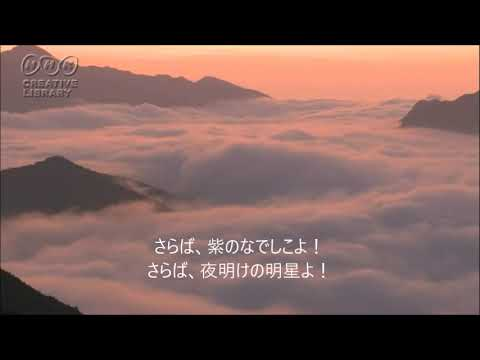
\includegraphics[width=0.48\linewidth]{pictures/youtube/2026/01/20260115_212950_youtube_001_mIOtV8KUQHE.jpg}
}
\end{center}

\subsection*{2026年01月17日 11:16}
\addcontentsline{toc}{subsection}{2026年01月17日 11:16}

\paragraph{リンク}
\url{https://youtu.be/ADtOPPxff_o}

\begin{center}
\href{https://youtu.be/ADtOPPxff_o}{
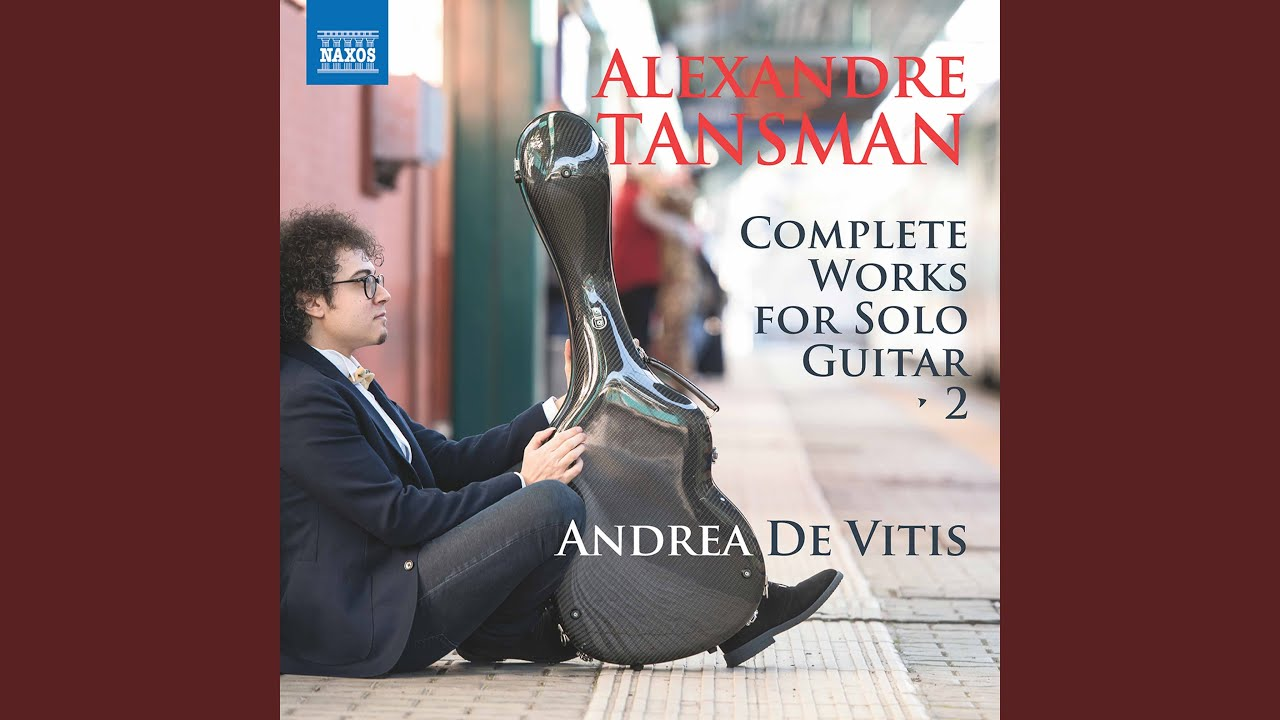
\includegraphics[width=0.48\linewidth]{pictures/youtube/2026/01/20260117_111645_youtube_001_ADtOPPxff_o.jpg}
}
\end{center}

\subsection*{2026年01月18日 05:47}
\addcontentsline{toc}{subsection}{2026年01月18日 05:47}

\paragraph{リンク}
\url{https://youtu.be/RLcSrQh6D1k}

\begin{center}
\href{https://youtu.be/RLcSrQh6D1k}{
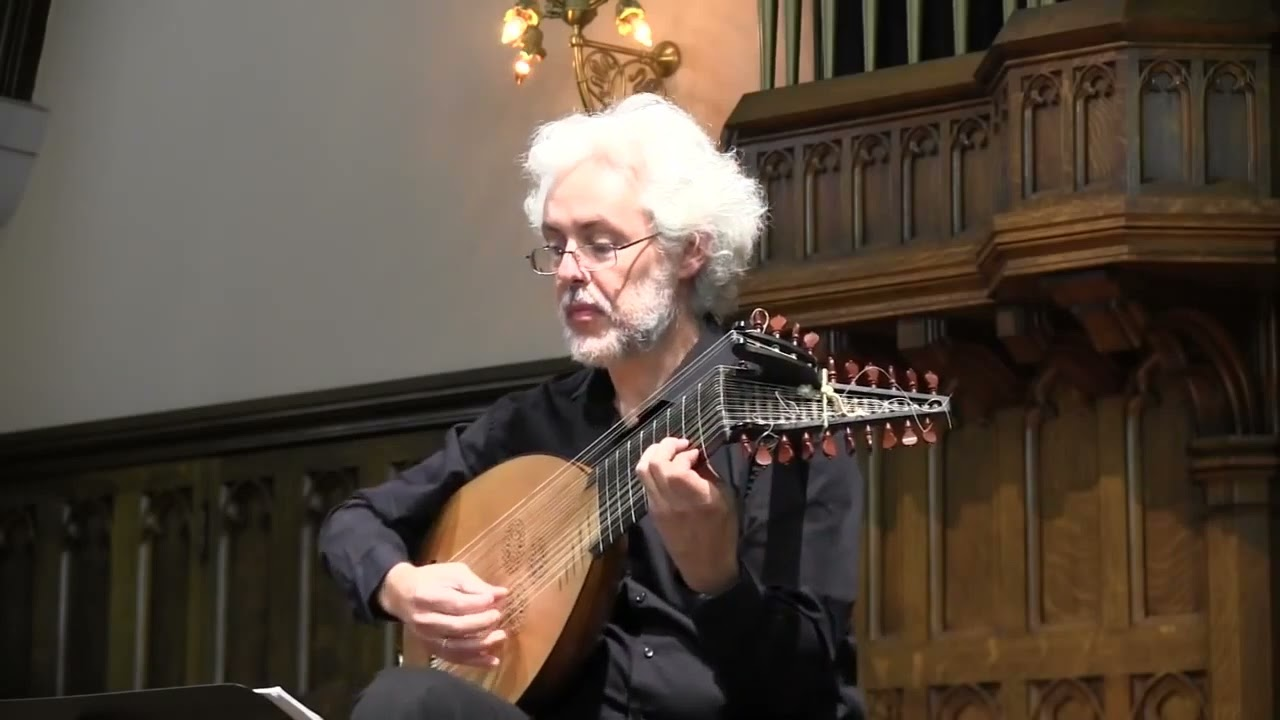
\includegraphics[width=0.48\linewidth]{pictures/youtube/2026/01/20260118_054700_youtube_001_RLcSrQh6D1k.jpg}
}
\end{center}

\subsection*{2026年01月18日 16:00}
\addcontentsline{toc}{subsection}{2026年01月18日 16:00}

Prelude, Fugue and Allegro（BWV998）のFugueの楽譜のために、添付の台紙↓を購入したのが昨年末の12月27日だった（28日か29日には届いていたでしょう）。シャイト編のFugueの楽譜は丁度４ページあるので、楽譜のコピーを台紙に糊で貼り付けて、それを譜面台に乗せれば準備Okです。ここまで準備しないと、最後まで止まらずに弾ける様になるという目標は達成できる訳がないじゃないか、と年末になってようやく思い至るようになったという訳です。（出版され製本されている楽譜をそのまま見て弾いていると言うことは、一旦弾くのを止めてページを捲るという動作を伴う事が前提になっている訳ですから）


今日は年も明けて2026年の1月18日です。BWV998のPreludeからFugueの終りまで、途中で止まらずに（初めて）弾き通す事ができました（記念日です）。ゆっくり、もちろん楽譜を見ながら、とにかく音が出ているというだけの、運指を確定できたと言うレベルですが、鳴らさない音などの誤魔化しのない事を心掛けています。本当は去年中に弾き通せる様にする目標だったのですが、年を越して今日までになってしまいました。

それにしても、実に長い曲です。1、2、3、4ページと演奏してきて、4ページ目の最後の小節、右下のD.S.（ダル セーニョ）から、1ページ目の1段目にあるセーニョに戻った時に、つくづく「長い！」って思いましたよ。曲が終わるのは2ページ目の2段目なのですから。


この記事は、以下↓の個人的プロジェクトの続きです。

\url{https://www.facebook.com/100002225117991/posts/25408145472176274/}




この段階にきて、やはりきちんと暗譜しなければダメなんだという思いを新たにしました。途中で止まると言う事は即ち「次の運指はどうだっけ」と思い出せない事に依って生じている訳ですから。Fugueは、ただでさえストレッチを要する運指（例えば、6弦fis-3弦a-1弦aの和音に続いて2弦dや3弦cを弾くなど）が頻出する上に、ハイポジションからの「複雑な運指『の連続』」が数ヶ所あります。それらの箇所をある程度覚えてしまわないと、今回たまたま止まらなかったというだけの事で、その内すぐに止まってしまう（＝次の運指を忘れている）様になるのは目に見えています。複数の声部を鳴らしたりディナーミクを付けたりなどは、まだまだ先の事ですね。

\paragraph{写真}
\begin{center}
\begin{minipage}{0.48\linewidth}
\centering
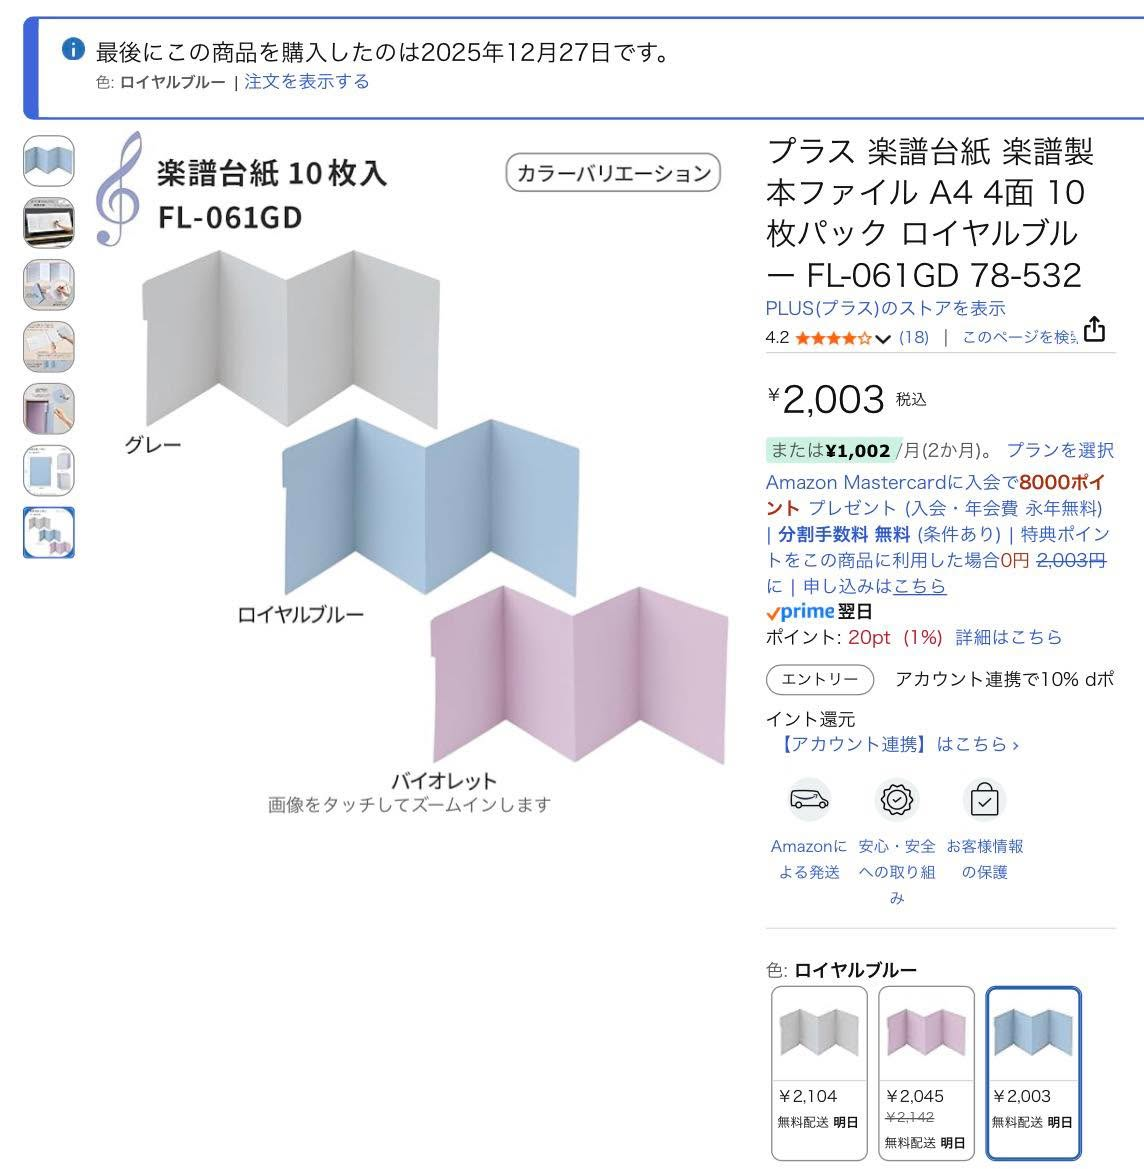
\includegraphics[width=\linewidth]{pictures/2026/01/20260118_160014_001.jpg}
\end{minipage}
\end{center}

\subsection*{2026年01月18日 19:29}
\addcontentsline{toc}{subsection}{2026年01月18日 19:29}

\paragraph{リンク}
\url{https://youtu.be/LVkyT5xcQsU}

\begin{center}
\href{https://youtu.be/LVkyT5xcQsU}{
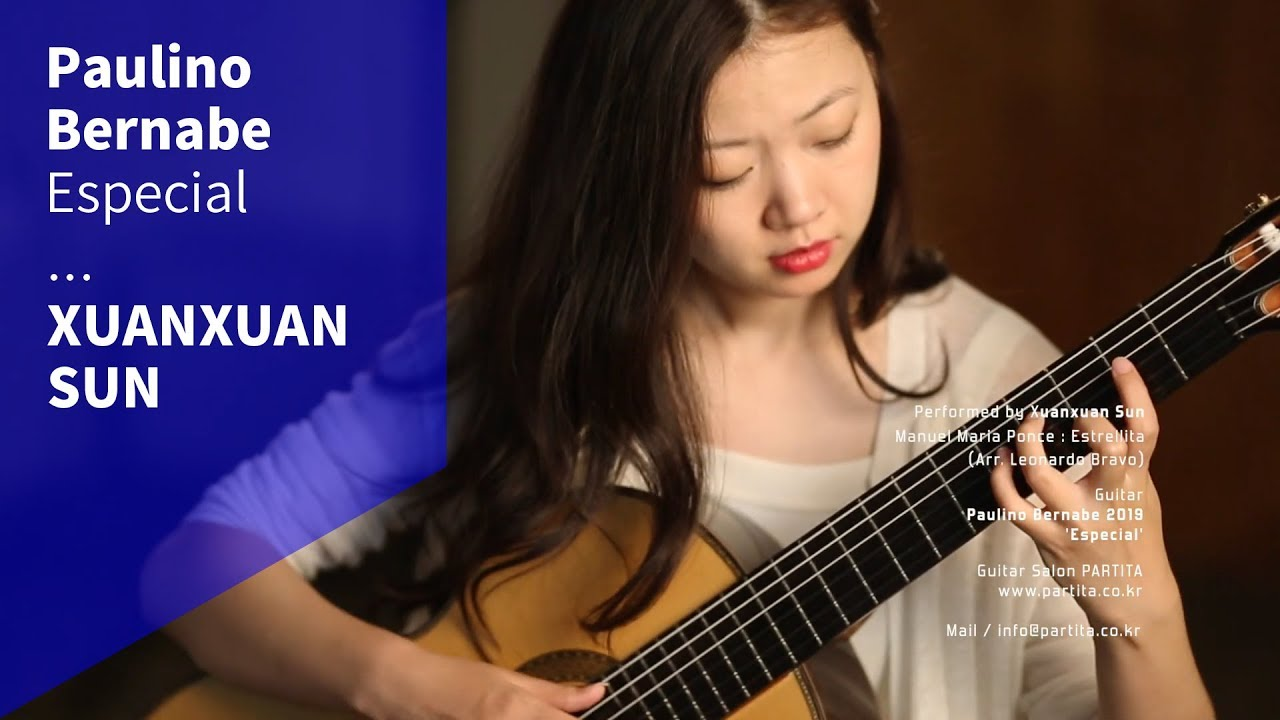
\includegraphics[width=0.48\linewidth]{pictures/youtube/2026/01/20260118_192940_youtube_001_LVkyT5xcQsU.jpg}
}
\end{center}

\subsection*{2026年01月19日 05:05}
\addcontentsline{toc}{subsection}{2026年01月19日 05:05}

\paragraph{リンク}
\url{https://youtu.be/UGQFnJDCRls}

\begin{center}
\href{https://youtu.be/UGQFnJDCRls}{
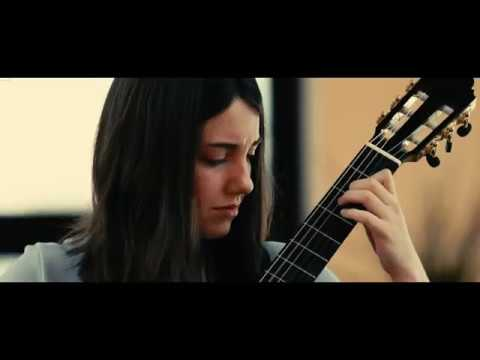
\includegraphics[width=0.48\linewidth]{pictures/youtube/2026/01/20260119_050516_youtube_001_UGQFnJDCRls.jpg}
}
\end{center}

\subsection*{2026年01月19日 09:01}
\addcontentsline{toc}{subsection}{2026年01月19日 09:01}

\paragraph{リンク}
\url{https://youtu.be/qbYmJA7kFX0}

\begin{center}
\href{https://youtu.be/qbYmJA7kFX0}{
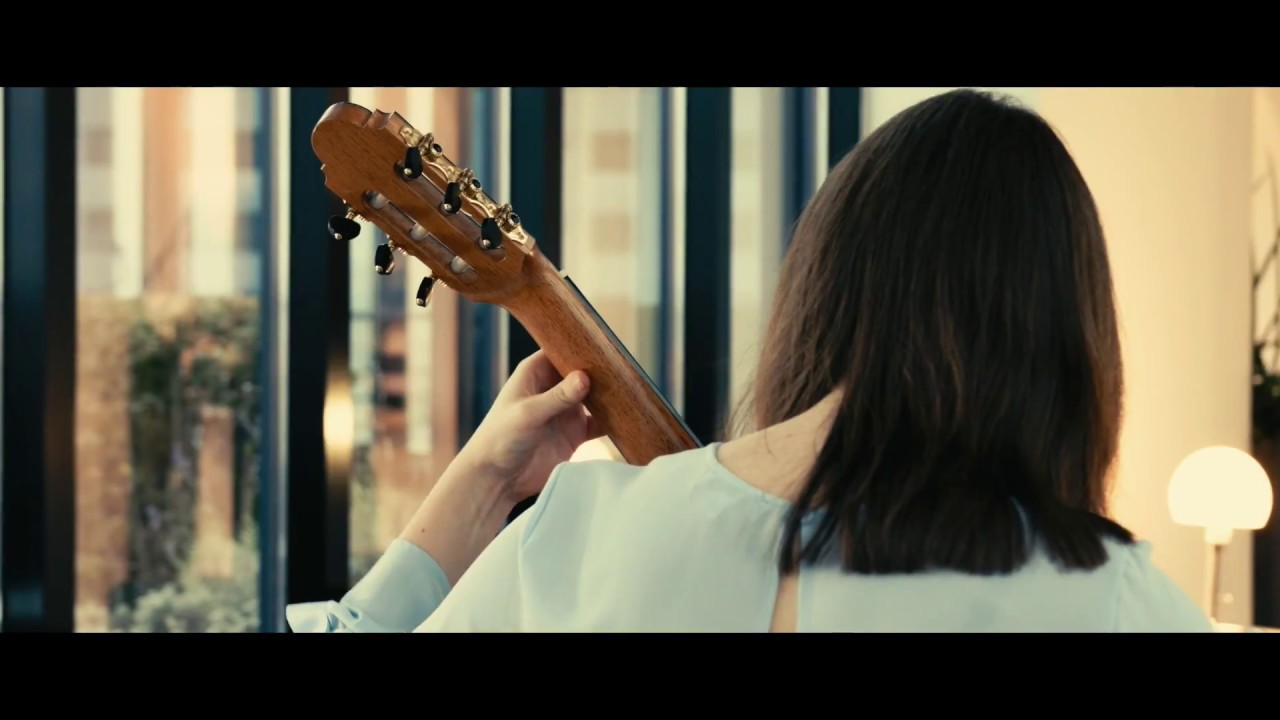
\includegraphics[width=0.48\linewidth]{pictures/youtube/2026/01/20260119_090129_youtube_001_qbYmJA7kFX0.jpg}
}
\end{center}

\subsection*{2026年01月19日 09:04}
\addcontentsline{toc}{subsection}{2026年01月19日 09:04}

\paragraph{リンク}
\url{https://youtu.be/ipx1rlvl66g}

\begin{center}
\href{https://youtu.be/ipx1rlvl66g}{
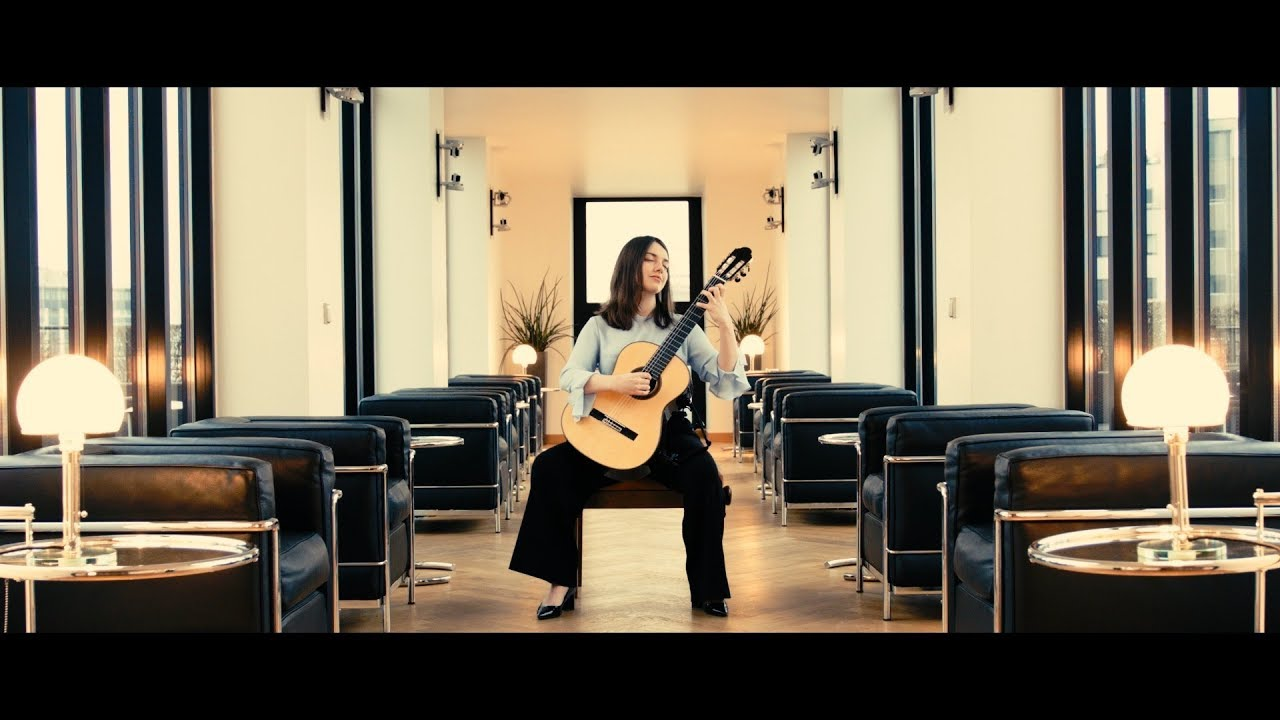
\includegraphics[width=0.48\linewidth]{pictures/youtube/2026/01/20260119_090407_youtube_001_ipx1rlvl66g.jpg}
}
\end{center}

\subsection*{2026年01月20日 09:10}
\addcontentsline{toc}{subsection}{2026年01月20日 09:10}

６つのPartitaより、１つ目のPartita（BWV825）


Prelude

\url{https://youtu.be/OabBda-0Q_A}

\begin{center}
\href{https://youtu.be/OabBda-0Q_A}{
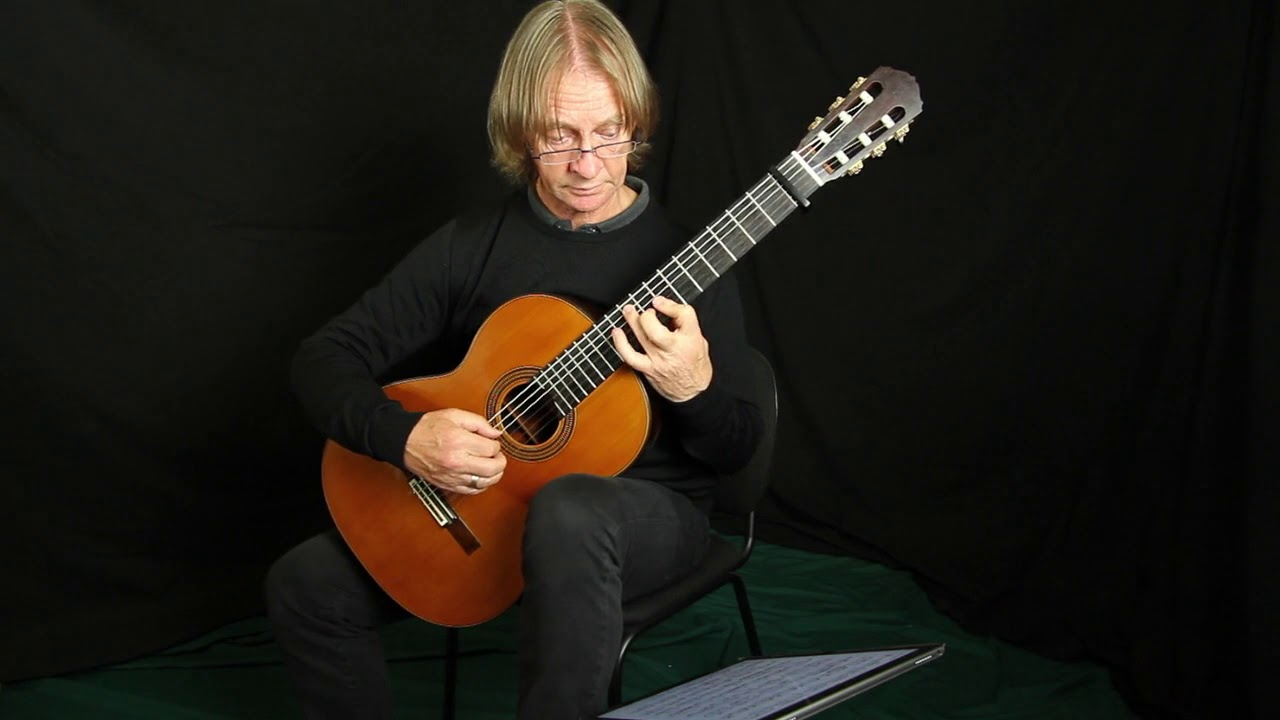
\includegraphics[width=0.48\linewidth]{pictures/youtube/2026/01/20260120_091047_youtube_001_OabBda-0Q_A.jpg}
}
\end{center}




Allemande

\url{https://youtu.be/RstVbCMK4_Y}

\begin{center}
\href{https://youtu.be/RstVbCMK4_Y}{
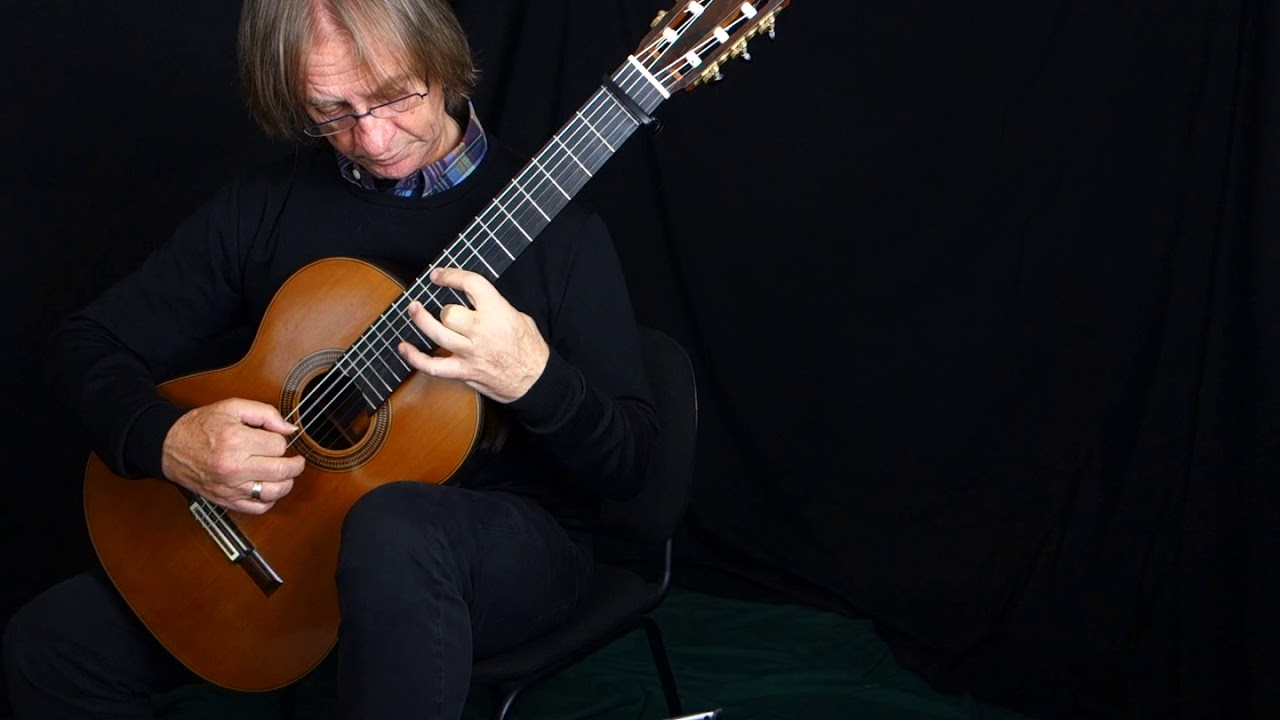
\includegraphics[width=0.48\linewidth]{pictures/youtube/2026/01/20260120_091047_youtube_002_RstVbCMK4_Y.jpg}
}
\end{center}




Courante

\url{https://youtu.be/RkKm9PpVZsQ}

\begin{center}
\href{https://youtu.be/RkKm9PpVZsQ}{
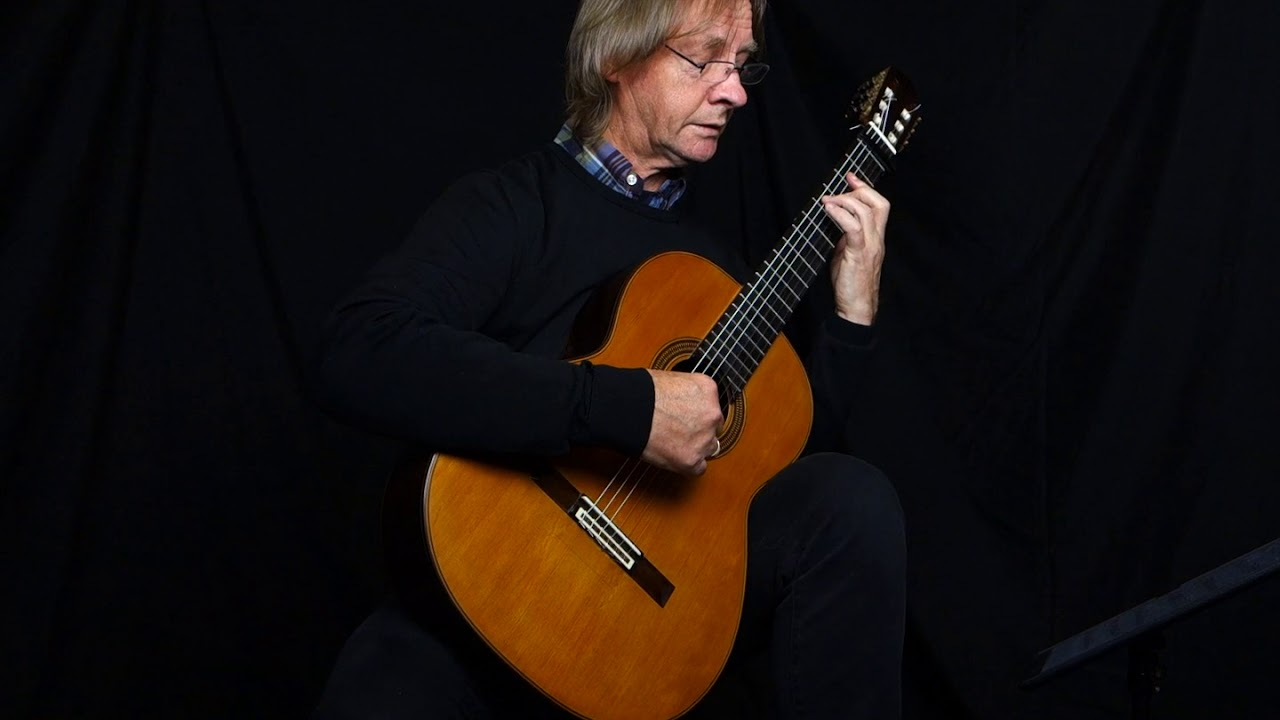
\includegraphics[width=0.48\linewidth]{pictures/youtube/2026/01/20260120_091047_youtube_003_RkKm9PpVZsQ.jpg}
}
\end{center}




Sarabande

\url{https://youtu.be/HgWldi02m2E}

\begin{center}
\href{https://youtu.be/HgWldi02m2E}{
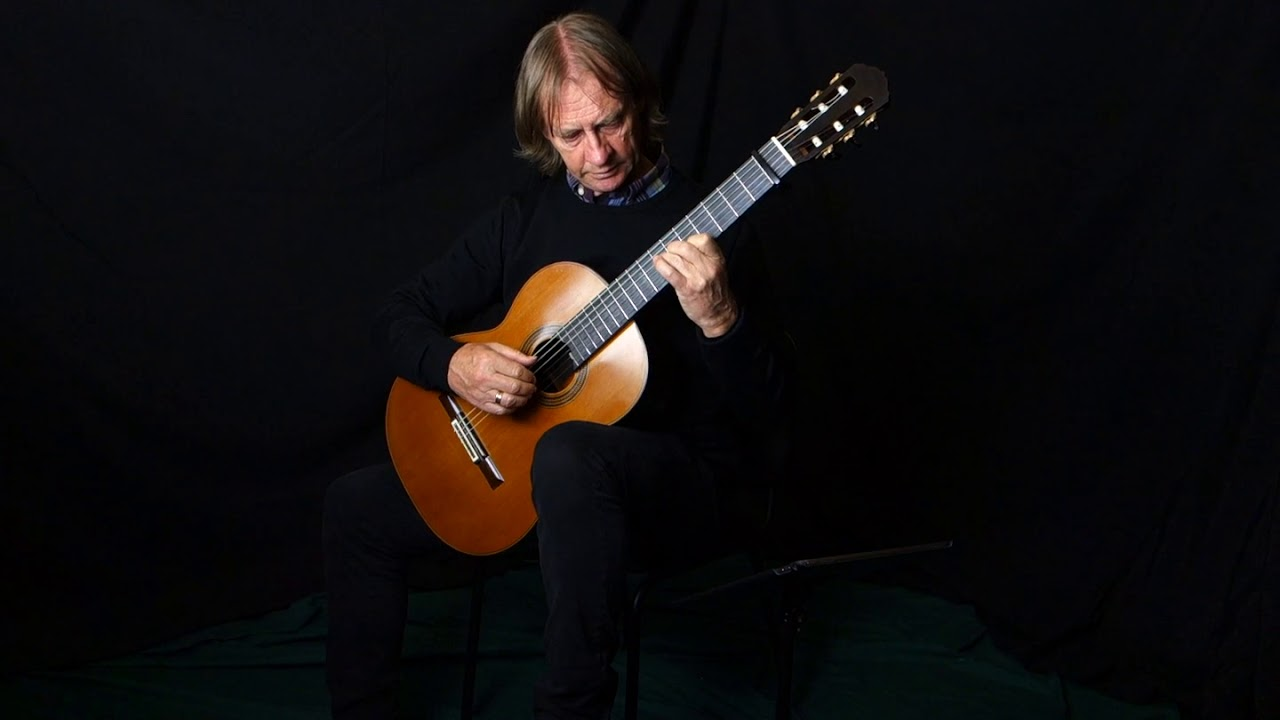
\includegraphics[width=0.48\linewidth]{pictures/youtube/2026/01/20260120_091047_youtube_004_HgWldi02m2E.jpg}
}
\end{center}




Minuets1,2

\url{https://youtu.be/1S0QNcjQybc}

\begin{center}
\href{https://youtu.be/1S0QNcjQybc}{
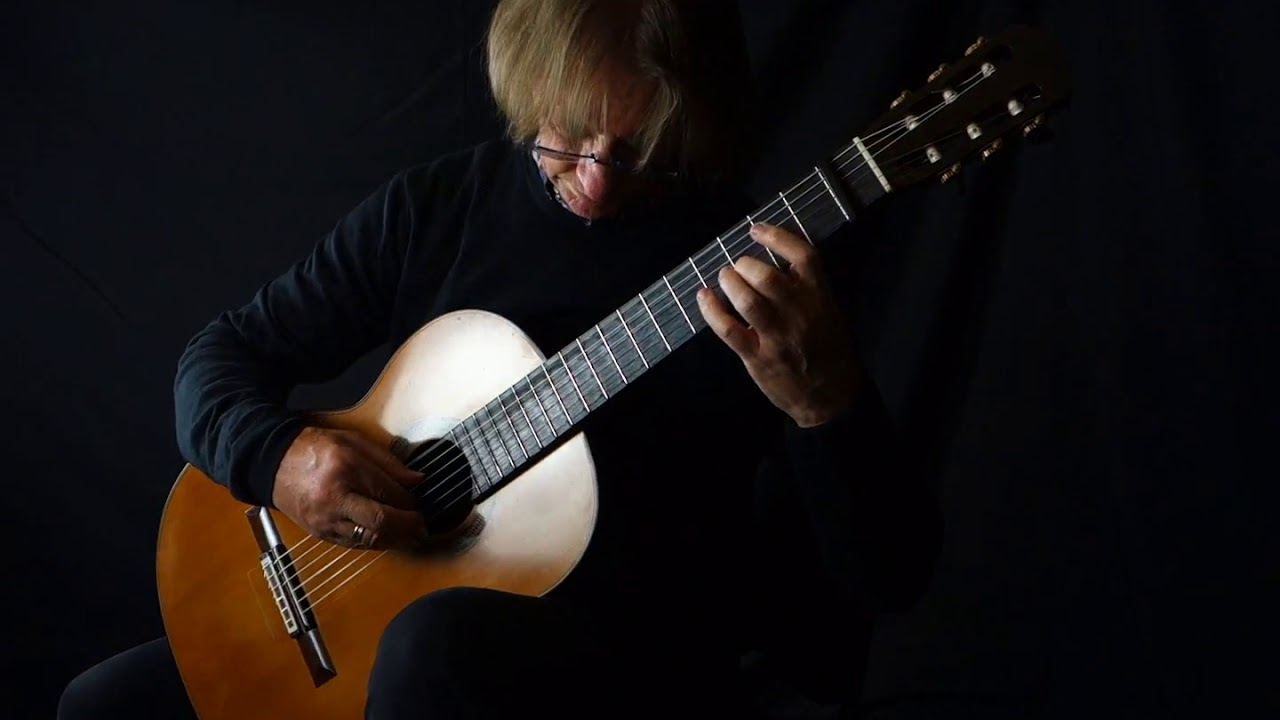
\includegraphics[width=0.48\linewidth]{pictures/youtube/2026/01/20260120_091047_youtube_005_1S0QNcjQybc.jpg}
}
\end{center}




Gigue

\url{https://youtu.be/bW2hyn8fnGc}

\begin{center}
\href{https://youtu.be/bW2hyn8fnGc}{
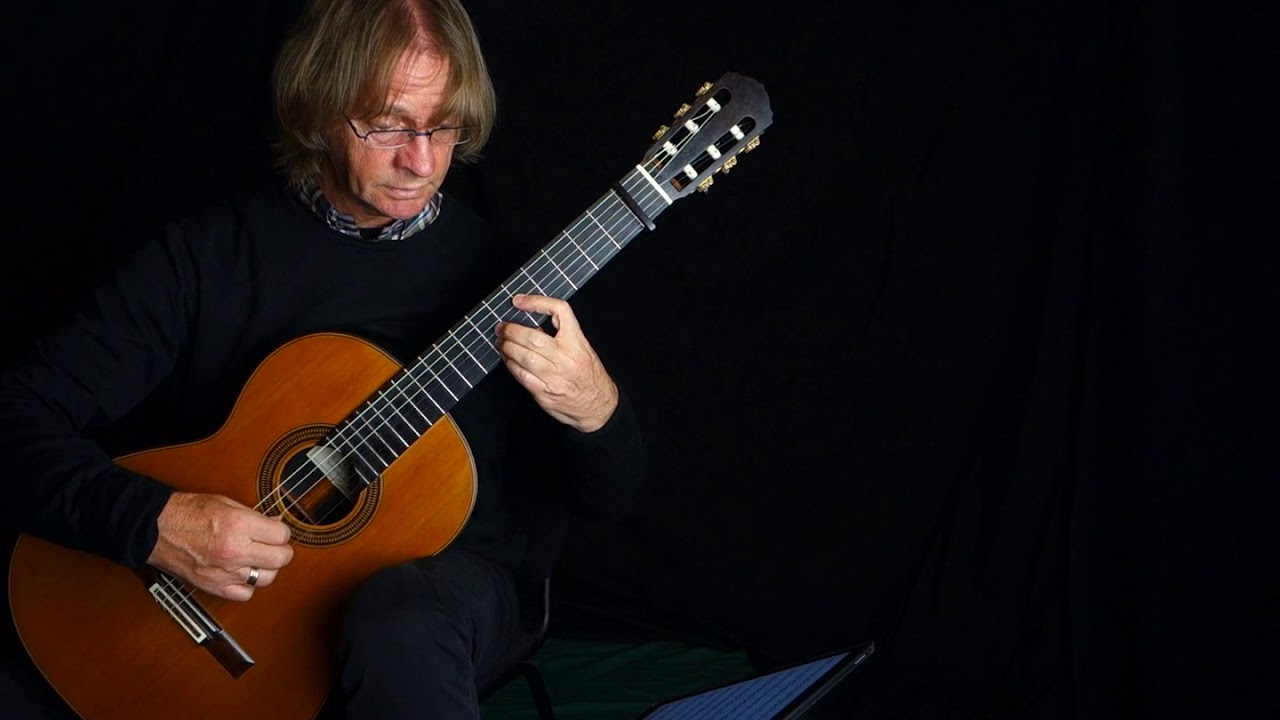
\includegraphics[width=0.48\linewidth]{pictures/youtube/2026/01/20260120_091047_youtube_006_bW2hyn8fnGc.jpg}
}
\end{center}



\subsection*{2026年01月21日 13:19}
\addcontentsline{toc}{subsection}{2026年01月21日 13:19}

無伴奏バイオリン パルティータ 第2番（BWV1004）より、アルマンド、クーラント、サラバンド、ジーグ

（シャコンヌが演奏されていないのは理解できます）

Allemande 

\url{https://youtu.be/PDV7T59IH34?t=13}

\begin{center}
\href{https://youtu.be/PDV7T59IH34?t=13}{
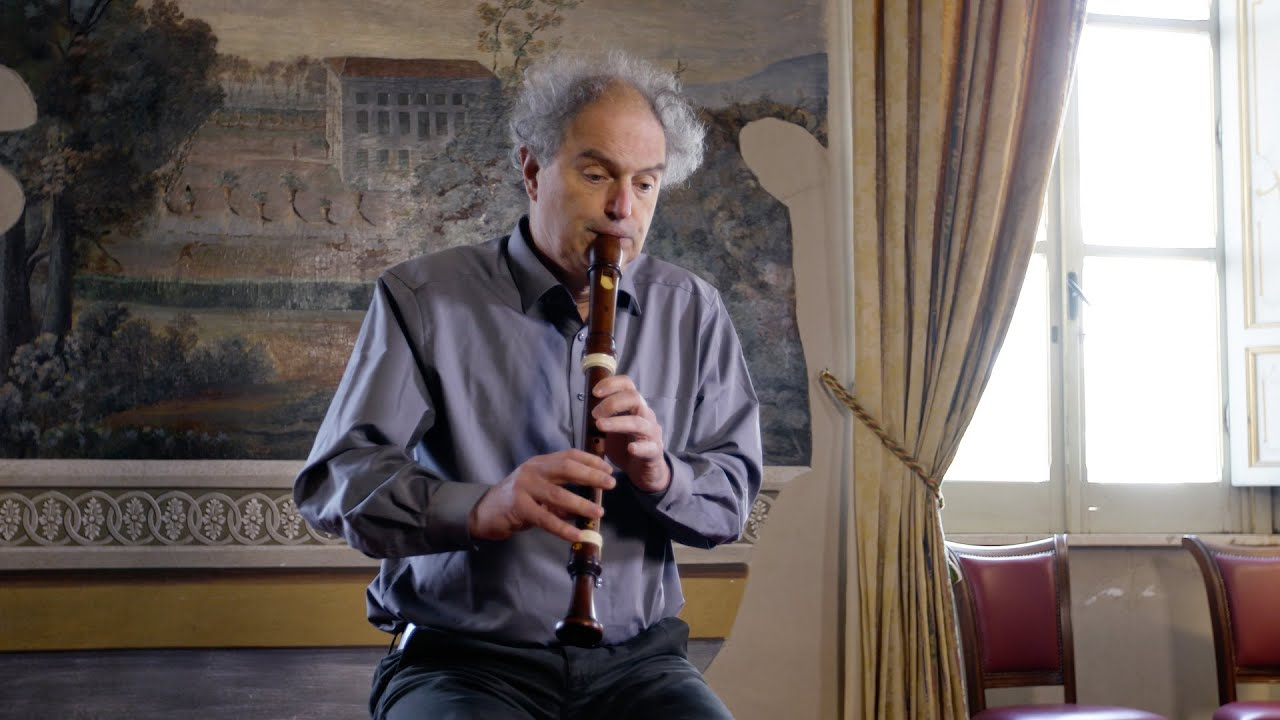
\includegraphics[width=0.48\linewidth]{pictures/youtube/2026/01/20260121_131945_youtube_001_PDV7T59IH34.jpg}
}
\end{center}



Corrente 

\url{https://youtu.be/PDV7T59IH34?t=393}



Sarabanda 

\url{https://youtu.be/PDV7T59IH34?t=569}



Giga 

\url{https://youtu.be/PDV7T59IH34?t=880}



編曲と演奏はダニエル・ブリュッヘン氏。この方は、フランス・ブリュッヘン氏の末裔でしょうか？（確かに顔つきは似ていらっしゃる様に思います）


フランス・ブリュッヘン氏は、BWV1004の中ではサラバンドをリコーダ用に編曲されている

\url{https://m.facebook.com/story.php?story_fbid=24491444063846424&id=100002225117991}




BWV1006（無伴奏バイオリン パルティータ 第3番）より、をリコーダで演奏をする方もいらっしゃる

\url{https://www.facebook.com/100002225117991/posts/24599080146416148/}




それにしてもリコーダのポテンシャルにはすごいものがあります

\url{https://youtu.be/PDV7T59IH34}



\subsection*{2026年01月23日 03:27}
\addcontentsline{toc}{subsection}{2026年01月23日 03:27}

これって、イタチごっこになっていないか？


\url{https://m.facebook.com/story.php?story_fbid=5689077101176404&id=100002225117991}



\paragraph{写真}
\begin{center}
\begin{minipage}{0.48\linewidth}
\centering
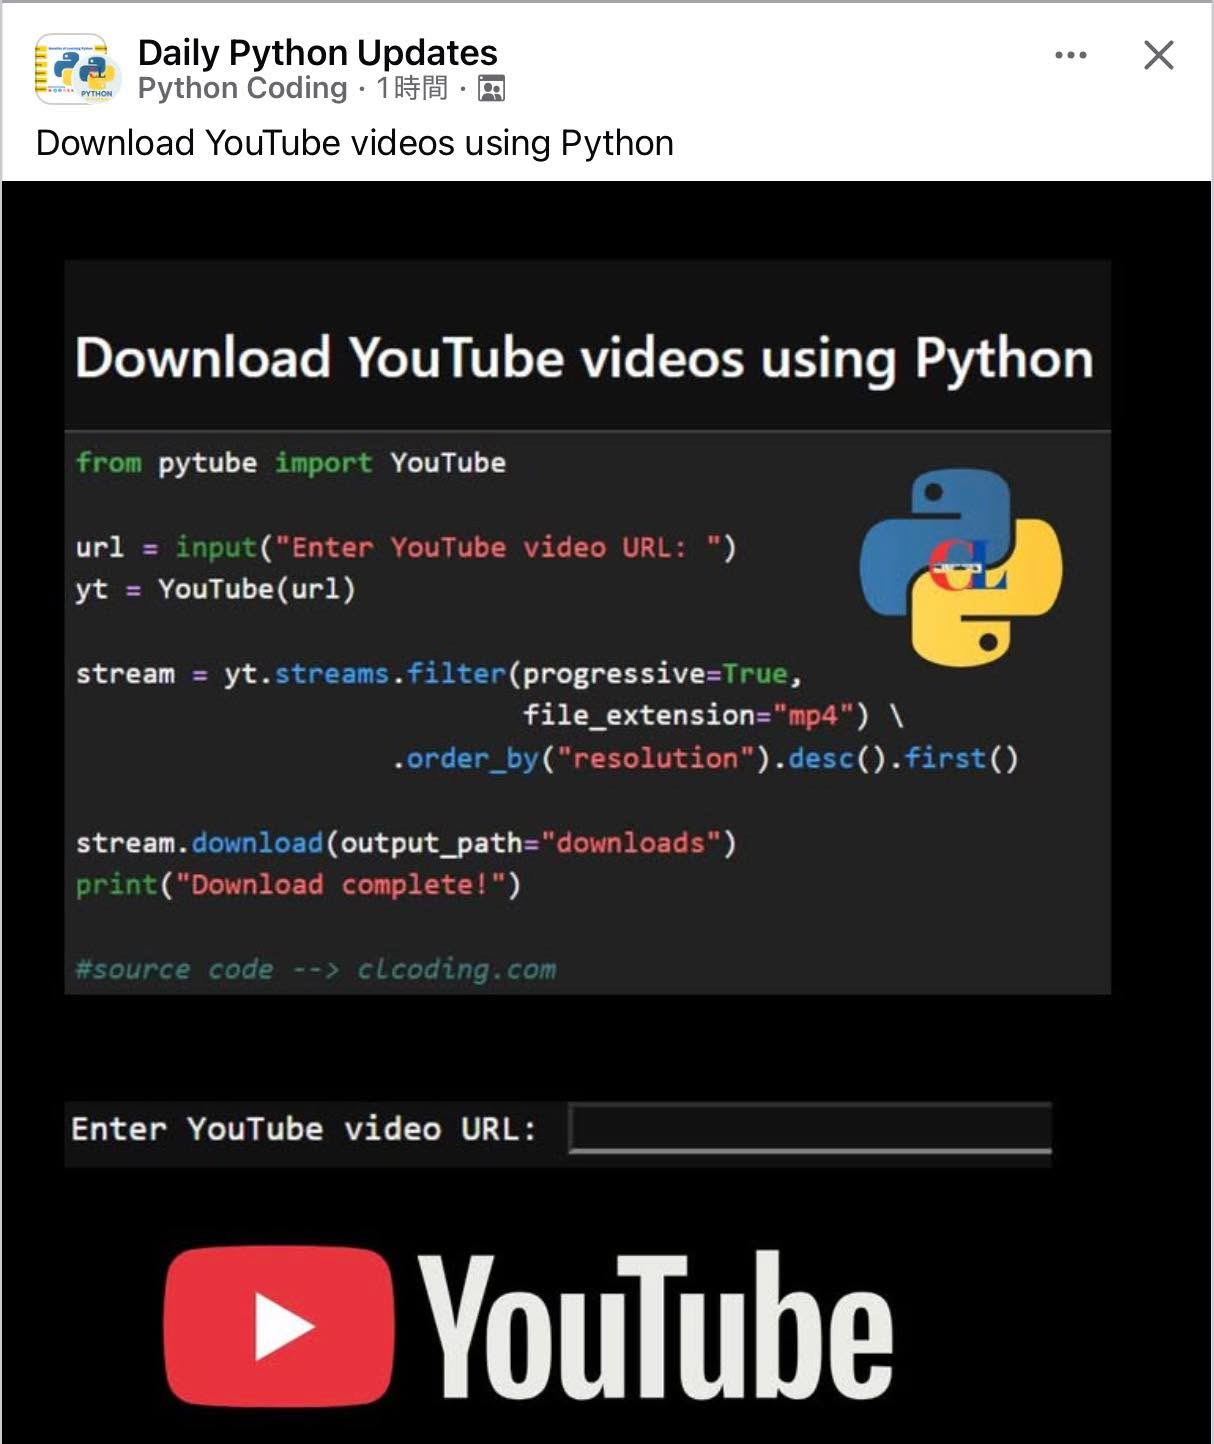
\includegraphics[width=\linewidth]{pictures/2026/01/20260123_032753_001.jpg}
\end{minipage}
\end{center}

\subsection*{2026年01月24日 06:22}
\addcontentsline{toc}{subsection}{2026年01月24日 06:22}

上の部分をドリッパ、下の部分をサーバと呼ぶらしい

ドリッパについて、一見シンプルそうだが、コーヒーの抽出に影響を与える要素が色々ある様です


(１)形：円錐形（HARIO）、台形（Kalita）

(２)角度：細長い（深い）、平たい（浅い）、V60

(３)下穴：サイズ（大中小）、数（1個〜複数個）

(４)材質：プラスティック、陶器（セラミック）、ガラス、金属

(５)壁面の溝：パターン（模様）、粗さ（細かさ）

(６)フィルタ：金属、布（ネル ドリップ）、紙（みさらし、漂白）、形（円錐形か台形か）

(７)ドリッパとサーバは、離れているか、接しているか


例えば、壁面の溝は空気が抜ける通路だとの事で、特にサーバと接している場合など抽出時間にも影響するため、その模様（溝の細かさや溝の捻れ具合なども）にはメーカーの工夫がある様だ。また、陶器やガラスの様な熱容量の大きな材質の場合、抽出の際に注がれるお湯の温度が大きく奪われるので、予めお湯で温めておく事（リンスと言うらしい）も行われるとの事。一方、陶器の場合一旦温まってしまうと温まった状態を比較的長めに維持できるので、ドリッパ内の温度ムラにはなりにくい様です。金属のドリッパの場合は熱が伝わりやすいので、暖まりやすく冷めやすい。さて、ドリッパ内の温度分布はどうだろうか。プラスティックが最も扱いやすいとの説もある。そして、フィルタが紙の場合、油分やコーヒー豆の細かい粉は通過しないが、金属や布のフィルタの場合には通過する事から（そもそも布或いは金属製のフィルタを通したコーヒーは濁っている）抽出後の味に直接影響するらしい。


陶器のドリッパで紙のフィルタが一般的↓なのか？試してみようと思っています


（その後）HARIOのセラミック製ドリッパ(02)とレンジ耐熱サーバ(02)、円錐形みさらし紙フィルタをAmazonでクリックしてしまいました。（HARIOではサイズの大、中、小を03、02、01と標記しているようです）購入に際しては、何故か（特に確信を伴った根拠も無かったのですが）セラミック材質とレンジ耐熱にこだわってしまいました。フィルタも漂白されていない方が良いような気がして選びました（漂白されていない代わりに着色されているかもしれませんが）。セットなら1082円↓で安めだったのですが、個別に選んだ事もあってやや高めについてしまいました。（この後、コーヒー豆とグラインダも要るのでは？）


=====

「コーヒーの味わい方の調査」の目次はここ↓

\url{https://www.facebook.com/100002225117991/posts/25623563003967852/}



\paragraph{写真}
\begin{center}
\begin{minipage}{0.48\linewidth}
\centering
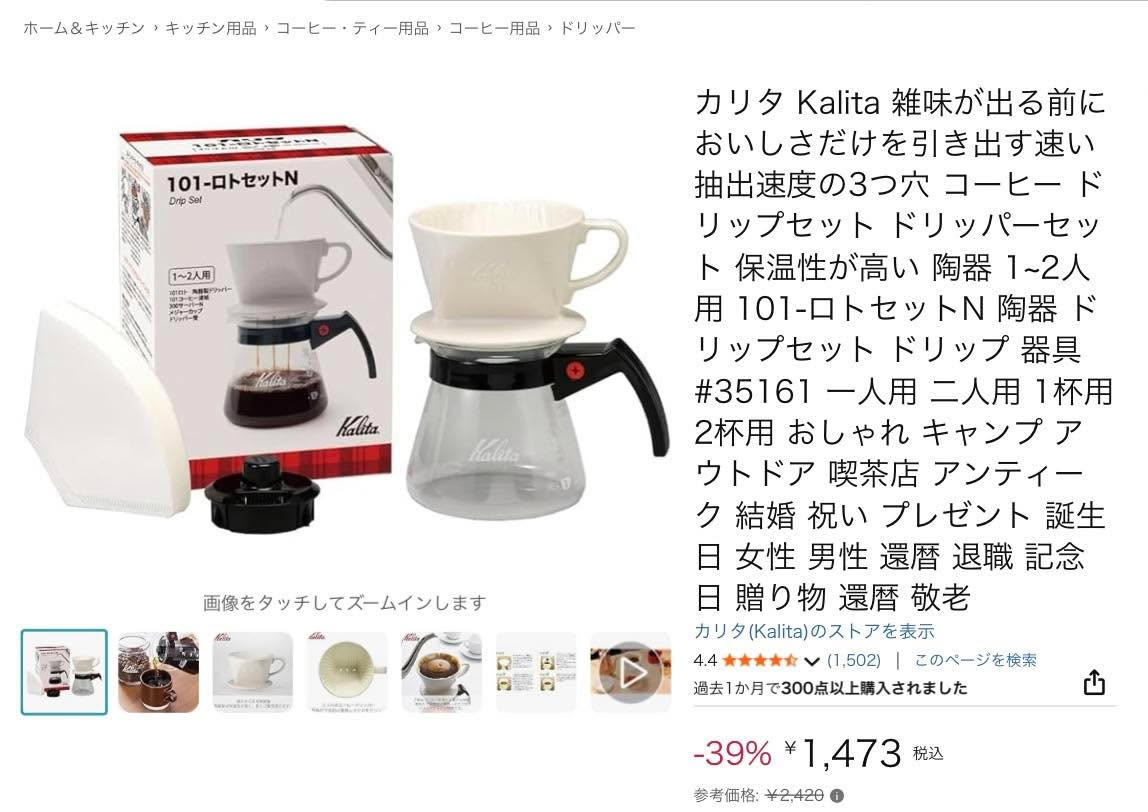
\includegraphics[width=\linewidth]{pictures/2026/01/20260124_062201_001.jpg}
\end{minipage}
\hfill
\begin{minipage}{0.48\linewidth}
\centering
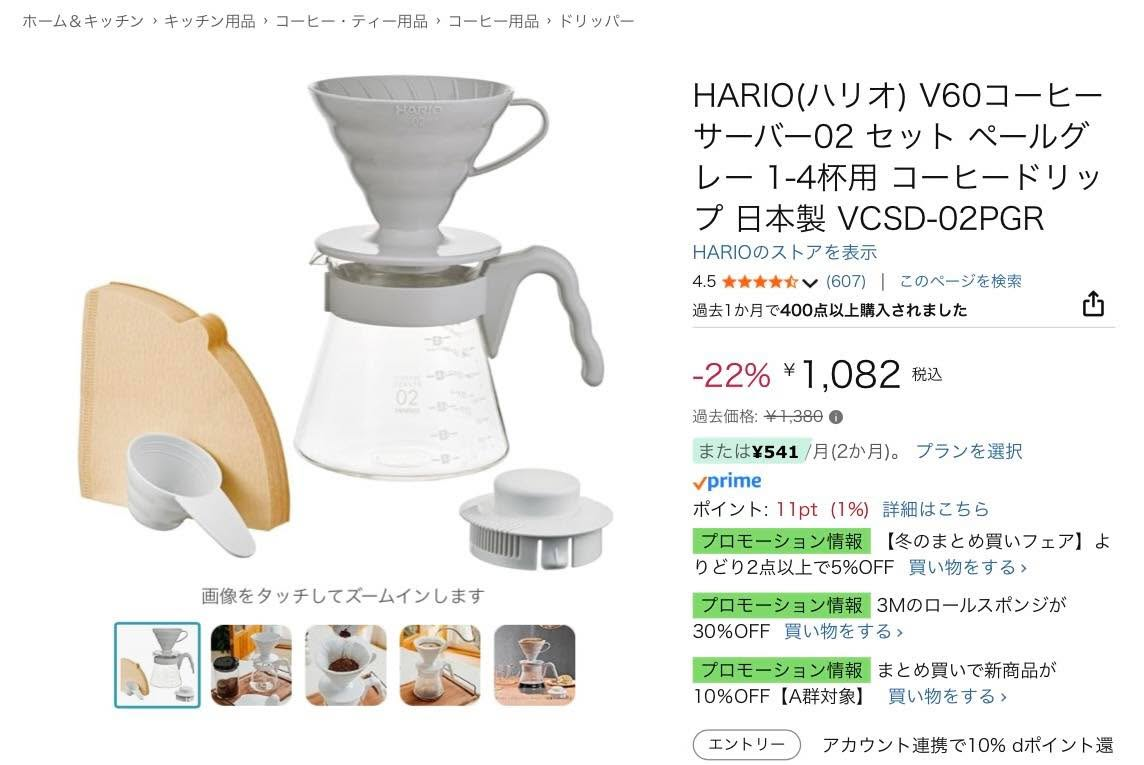
\includegraphics[width=\linewidth]{pictures/2026/01/20260124_062201_002.jpg}
\end{minipage}
\end{center}

\subsection*{2026年01月25日 02:41}
\addcontentsline{toc}{subsection}{2026年01月25日 02:41}

コーヒー豆の選択

押さえておくべき四つの産地


(１)ブラジル産は、

バランスが良く、香ばしい、ナッツの様な味わい

（迷ったらコレ）


(２)コロンビア産は、

しっかりしたコクと、柔らかい（バターやヨーグルトの様な乳酸系の）酸味

（スッパイのが嫌な方にお勧め）


(３)エチオピア産「モカ」は、

何と言っても香り（お花やフルーツの様な）が良く、華やか


(４)タンザニア産「キリマンジャロ」は、

しっかりとした（柑橘系のレモンやライムの様な）酸味

（キリッとした酸が好きな方にお勧め）


この情報は、UCCコーヒー アカデミー（Youtube↓）からの受け売りです

\url{https://youtu.be/dPra-TVGqvU}

\begin{center}
\href{https://youtu.be/dPra-TVGqvU}{
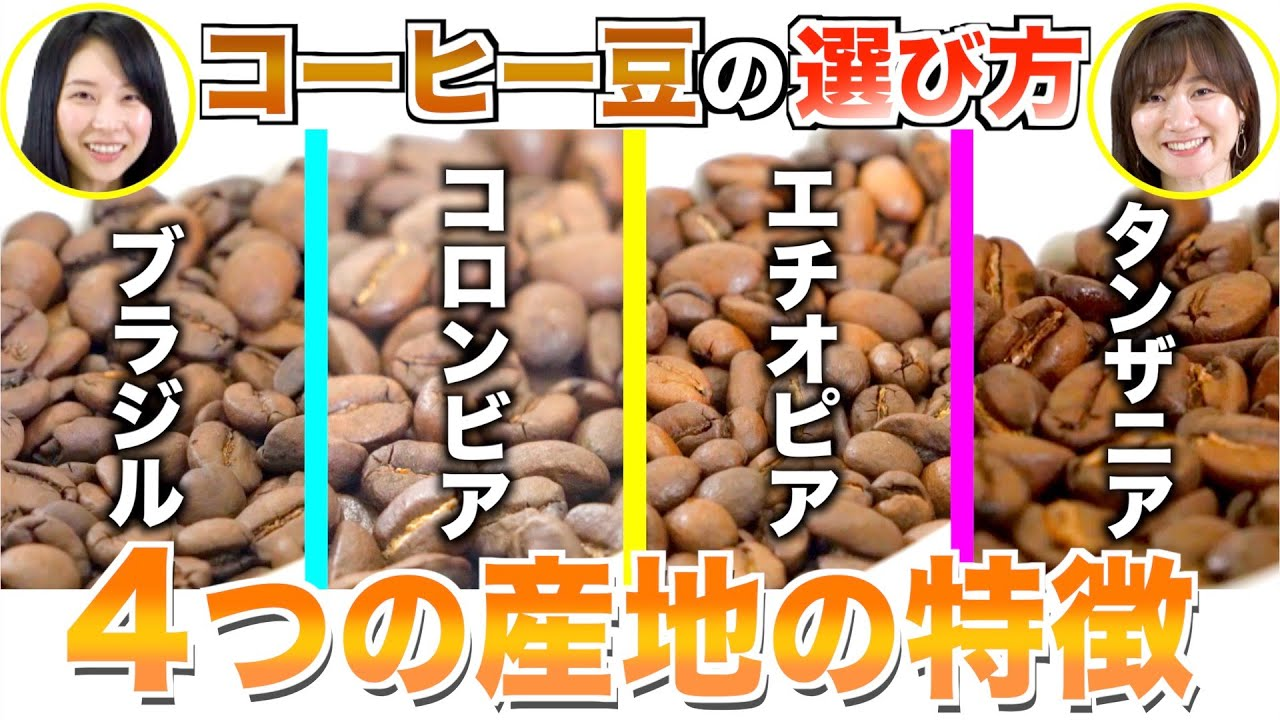
\includegraphics[width=0.48\linewidth]{pictures/youtube/2026/01/20260125_024119_youtube_001_dPra-TVGqvU.jpg}
}
\end{center}




=====

「コーヒーの味わい方の調査」の目次はここ↓

\url{https://www.facebook.com/100002225117991/posts/25623563003967852/}



\subsection*{2026年01月25日 03:31}
\addcontentsline{toc}{subsection}{2026年01月25日 03:31}

コーヒーの味わい方の調査

（ドリッパ＋サーバ＋ミル＋スケール＝¥27,591）


(１)コーヒー抽出器具（ドリッパとサーバ）

（HARIOドリッパ02¥1,400、HARIOサーバ02¥2,027）

\url{https://m.facebook.com/story.php?story_fbid=25614665554857597&id=100002225117991}




(２)コーヒー豆の選択

\url{https://www.facebook.com/100002225117991/posts/25623198760670943/}




(３)豆の粉砕度合いと粉砕用器具

（Epeiosミル¥18,480）

\url{https://www.facebook.com/100002225117991/posts/25623873190603500/}




(４)コーヒー抽出のプロセスと計測器具

（HARIOスケール¥5,684）

\url{https://www.facebook.com/100002225117991/posts/25624817673842385/}




(５)コーヒー抽出器具（サイフォン）

（HARIOの電熱器サイフォン¥12,500）

\url{https://www.facebook.com/100002225117991/posts/25658747500449402/}




(６)豆の炒り方と器具

ココには関わらない事にする


（７）用語：ブレンドとシングル オリジン、デカフェとは

\url{https://www.facebook.com/100002225117991/posts/25623699717287514/}




(８)コーヒーの味について

\url{https://www.facebook.com/100002225117991/posts/25643195212004631/}




(９)Switch用レシピ

(HARIO ¥4,950)

\url{https://www.facebook.com/100002225117991/posts/26509274735396670/}



\subsection*{2026年01月25日 03:51}
\addcontentsline{toc}{subsection}{2026年01月25日 03:51}

コーヒーに係る用語について調べました


シングル オリジン（Single Origin）

(１)豆：単一産地

(２)味：個性が際立つ

(３)安定性：年ごとに変わる

(４)楽しみ方：テイスティング


ブレンド（Blended）

(１)豆：複数産地

(２)味：バランス重視

(３)安定性：安定

(４)楽しみ方：日常使い


ブリュー レシオ（Brew Ratio）は、コーヒーの粉と湯の量の比率の事

\url{https://youtu.be/7VbkkwvFGQY}

\begin{center}
\href{https://youtu.be/7VbkkwvFGQY}{
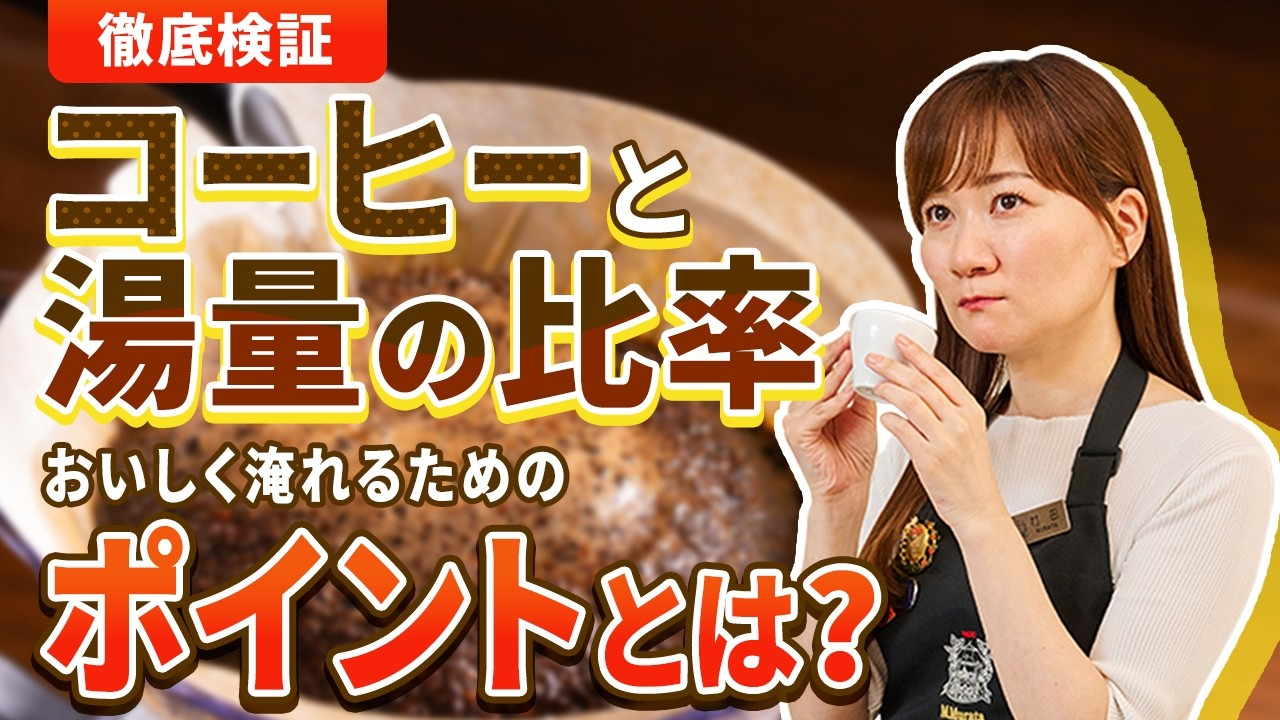
\includegraphics[width=0.48\linewidth]{pictures/youtube/2026/01/20260125_035115_youtube_001_7VbkkwvFGQY.jpg}
}
\end{center}




カフェイン レスはデカフェ（decaf＝「decaffeinated」の略）と同じ意味らしい。本来カフェインを含む飲料から、特殊な方法でカフェインを90\%〜99\%以上除去したものとの事。含有量は0\%ではないが、妊娠中や就寝前、カフェインを控えたい人でも、すっきりした味わいでコーヒーの香りを楽しめるという事らしい。ノン カフェイン飲料と言う言葉は、カフェイン0\%の飲み物の事を指しているが、コーヒーにはノン カフェインのものは無いとの事です。（

\url{https://youtu.be/Y_ag2Tx3TIY}

\begin{center}
\href{https://youtu.be/Y_ag2Tx3TIY}{

\includegraphics[width=0.48\linewidth]{pictures/youtube/2026/01/20260125_035115_youtube_002_Y_ag2Tx3TIY.jpg}
}
\end{center}

）


Single OriginのDecafを、以下↓で購入してみました

(１)カフェインを除去する処理に化学物質（ジクロロメタン等）を使っていない

(２)豆の栽培に農薬を使っていない（JAS認定オーガニック）

この２つが重要なポイントですが、さて美味しいのかな？


こんな紹介記事もある

\url{https://every-coffee.com/article/decafe.html}



\url{https://www.sotcoffee.com/collections/decaf}




=====

「コーヒーの味わい方の調査」の目次はここ↓

\url{https://www.facebook.com/100002225117991/posts/25623563003967852/}



\paragraph{写真}
\begin{center}
\begin{minipage}{0.48\linewidth}
\centering
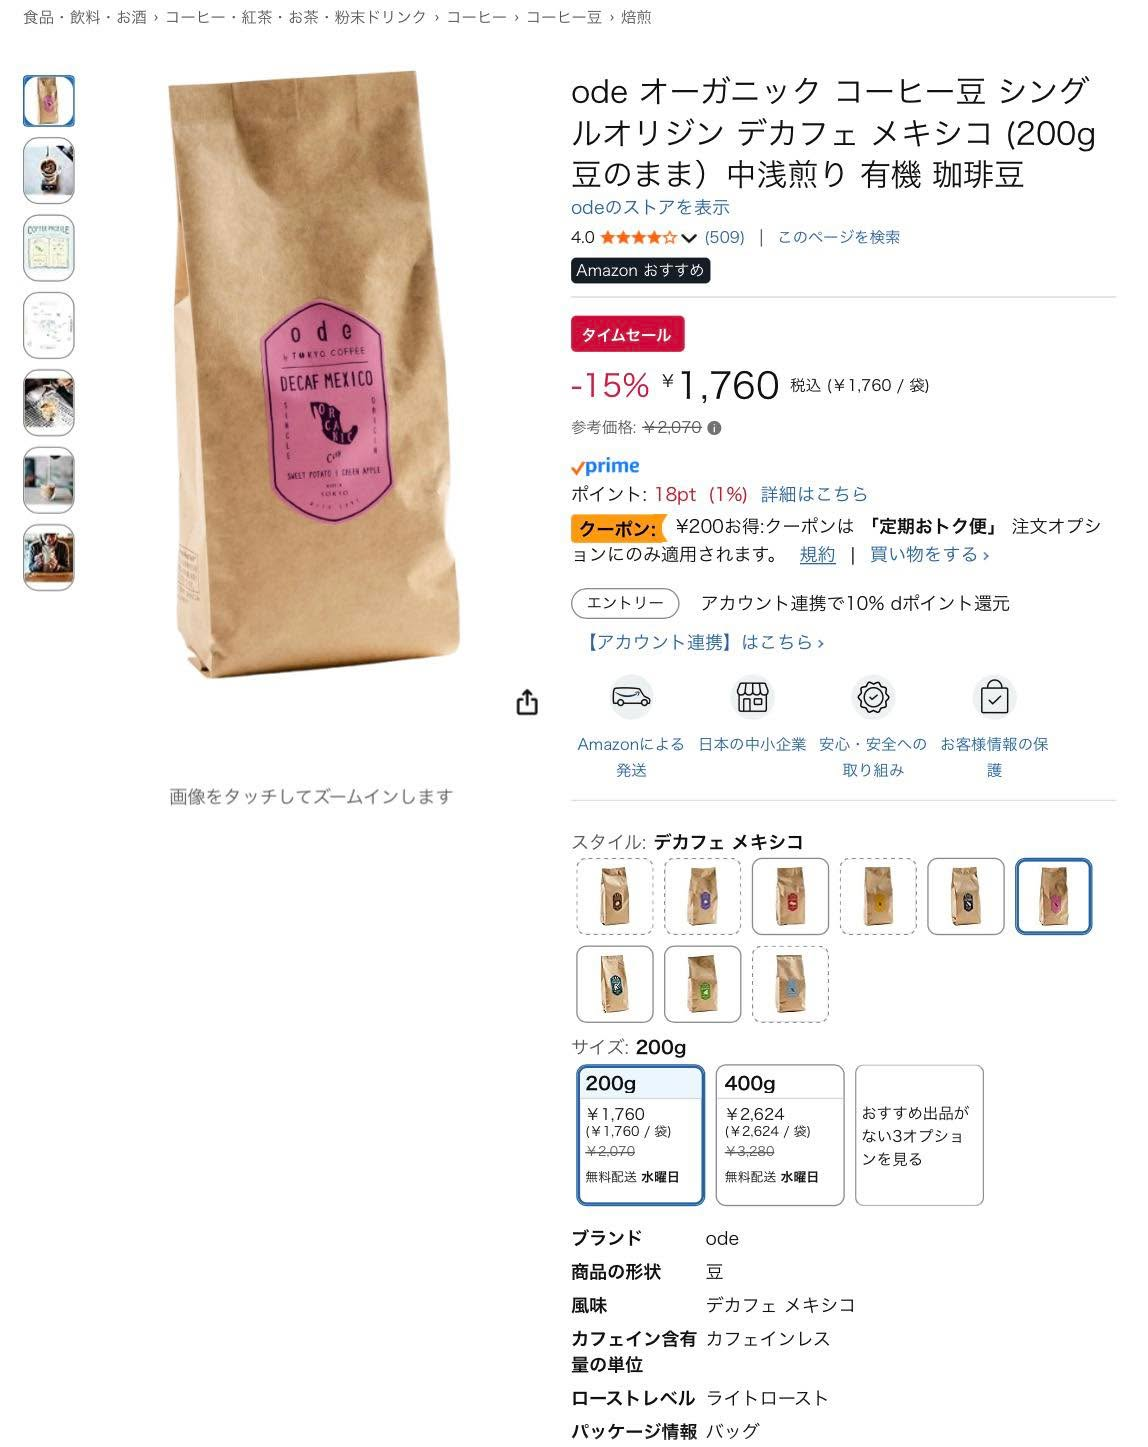
\includegraphics[width=\linewidth]{pictures/2026/01/20260125_035115_001.jpg}
\end{minipage}
\end{center}

\subsection*{2026年01月25日 04:17}
\addcontentsline{toc}{subsection}{2026年01月25日 04:17}

コーヒー豆の粉砕


(１)器具


コマンダンテとか言うブランド製品の金額（¥69,800）にはびっくり！

（細かいステップでの粒度設定が可能で、粒が揃っているらしいが、これは買えないワ）


Amazon限定タイムセールのKalita製（¥3,132）は以前から持っていたので使っていたのですが、一体今どんな粒度に設定しているのか分からないため、キチンとした検証ができない事が大きなストレスになってきました


結局Epeiosのミル↓をこの金額（¥18,480）で高いけどやむを得ず「妥協」購入してしまいました。金額には妥協でしたが、器具の性能としては、粒度を80段階で細かく設定できて、高級感溢れる品質の器具で満足です


(２)粒度


ネット上で市販のミル毎に、豆の粒度と対応する目盛の値との対応表を公開している方がいらっしゃいました。これに従ってEpeiosミルの設定を45にして試した所、喉にガサガサしてかなり濃い様に感じたので、これは細かすぎなんだと思い、55に設定し直して試してみている所です。（¥3,132のミルでは、こんな事ができなかったんですよね）豆はコロンビア、サイフォンで3杯分、豆と水の重量比（Brew Ratio）は1：16.5で試しています


\url{https://youtu.be/cIfmod04sUk}

\begin{center}
\href{https://youtu.be/cIfmod04sUk}{
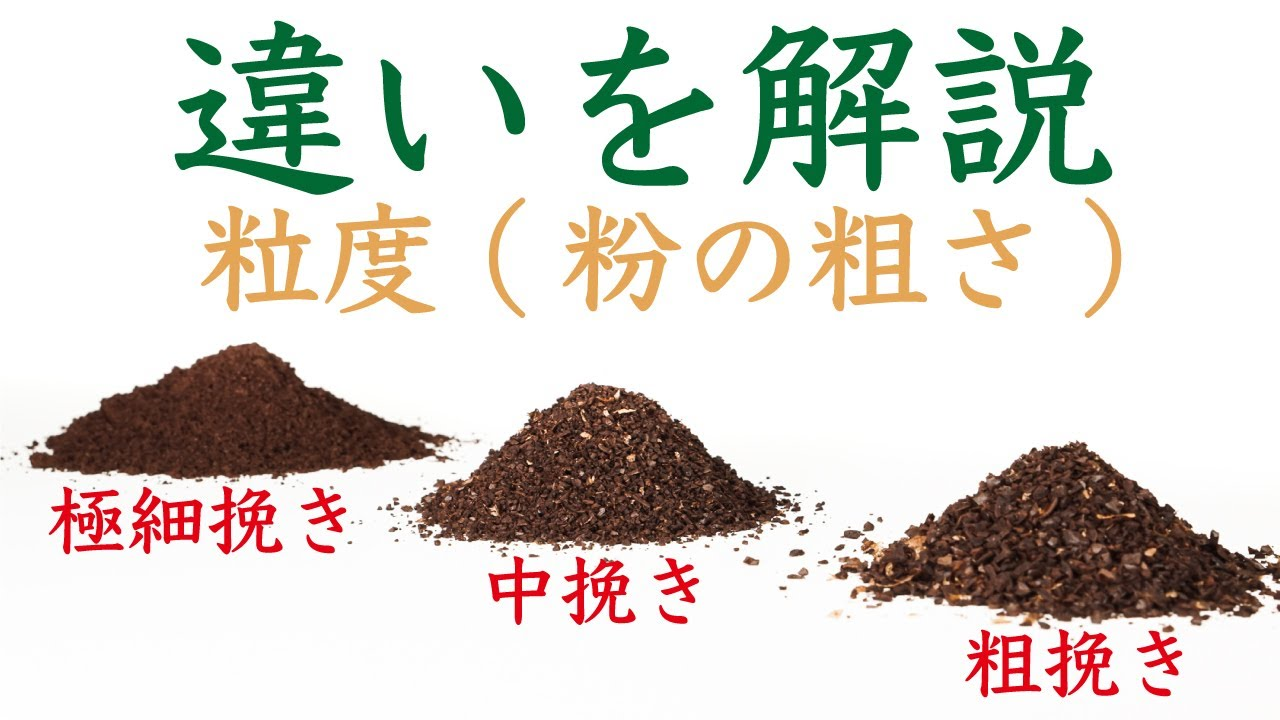
\includegraphics[width=0.48\linewidth]{pictures/youtube/2026/01/20260125_041717_youtube_001_cIfmod04sUk.jpg}
}
\end{center}




=====

「コーヒーの味わい方の調査」の目次はここ↓

\url{https://www.facebook.com/100002225117991/posts/25623563003967852/}



\paragraph{写真}
\begin{center}
\begin{minipage}{0.48\linewidth}
\centering
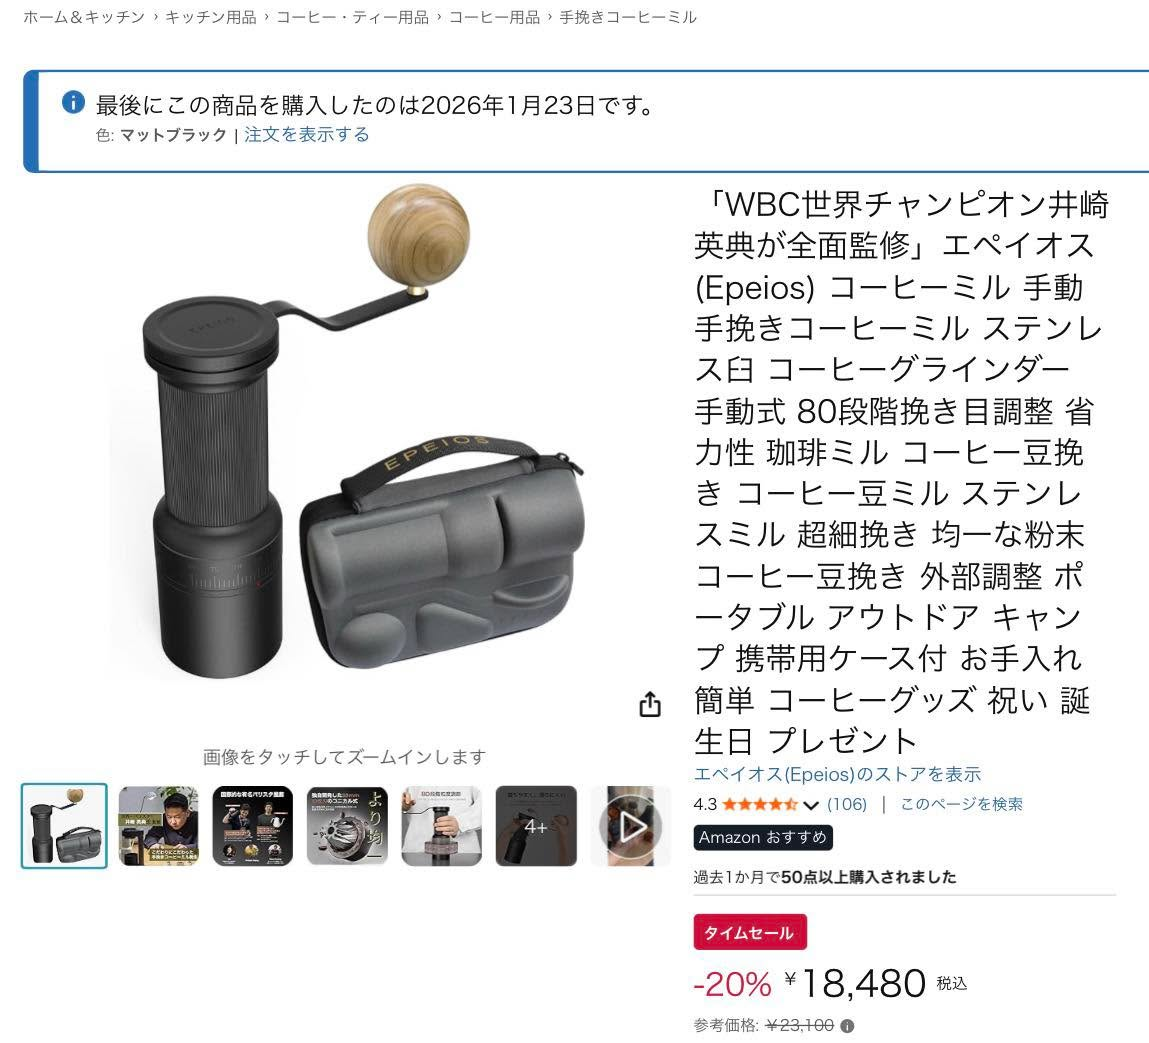
\includegraphics[width=\linewidth]{pictures/2026/01/20260125_041717_001.jpg}
\end{minipage}
\hfill
\begin{minipage}{0.48\linewidth}
\centering
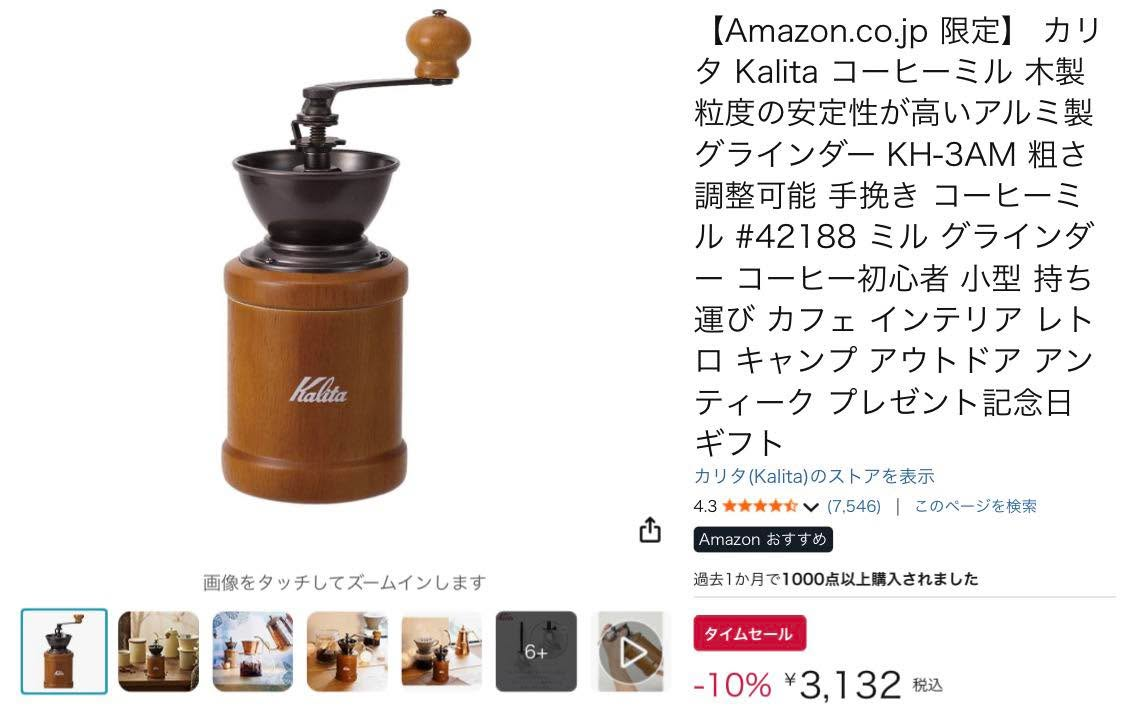
\includegraphics[width=\linewidth]{pictures/2026/01/20260125_041717_002.jpg}
\end{minipage}
\end{center}

\begin{center}
\begin{minipage}{0.48\linewidth}
\centering
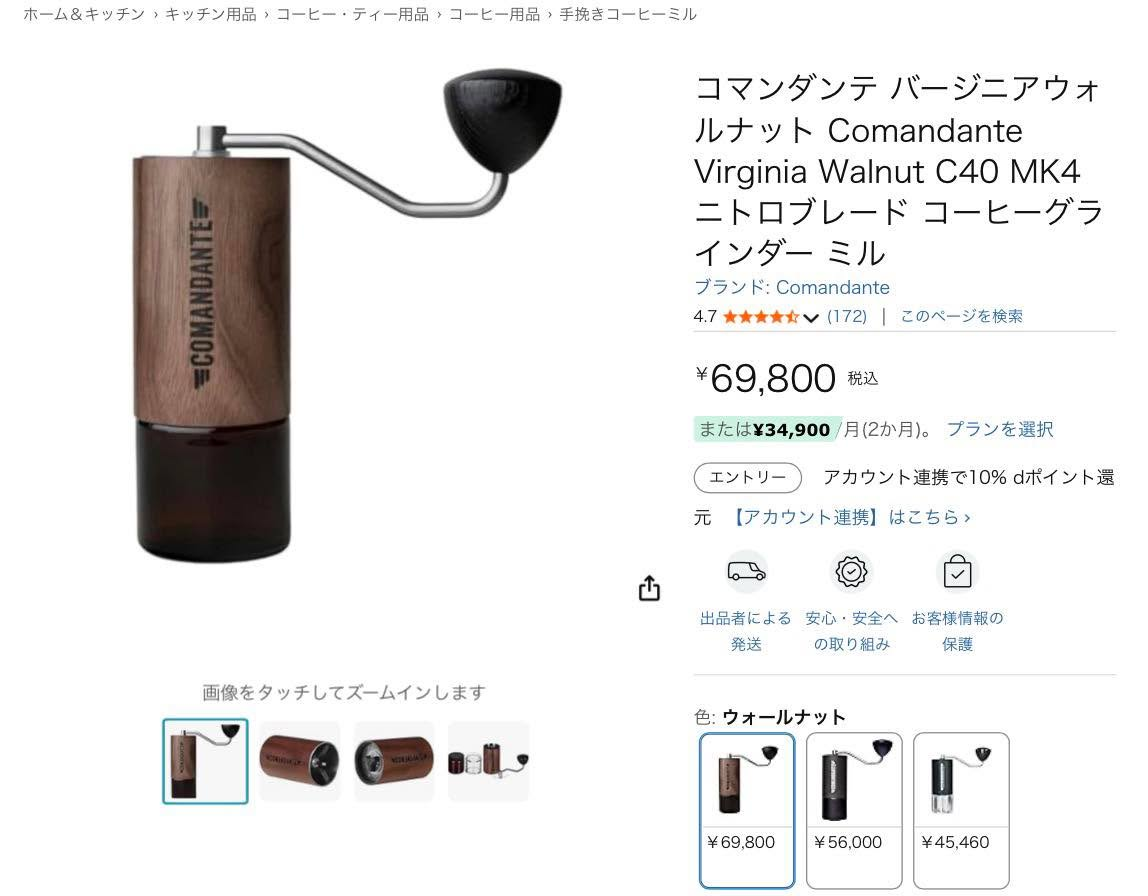
\includegraphics[width=\linewidth]{pictures/2026/01/20260125_041717_003.jpg}
\end{minipage}
\end{center}

\subsection*{2026年01月25日 06:52}
\addcontentsline{toc}{subsection}{2026年01月25日 06:52}

コーヒー抽出プロセス


(１)抽出プロセス管理器具


HARIOのポラリスという計器は、コーヒーの抽出に特化した優れた機能を持っている。コーヒーの粉と水の重量、及びそれら２つの間の比率を実時間で表示してくれる。更に抽出の経過時間も表示されるという優れものだ。


\url{https://youtu.be/4Ht3xvT-87k}

\begin{center}
\href{https://youtu.be/4Ht3xvT-87k}{
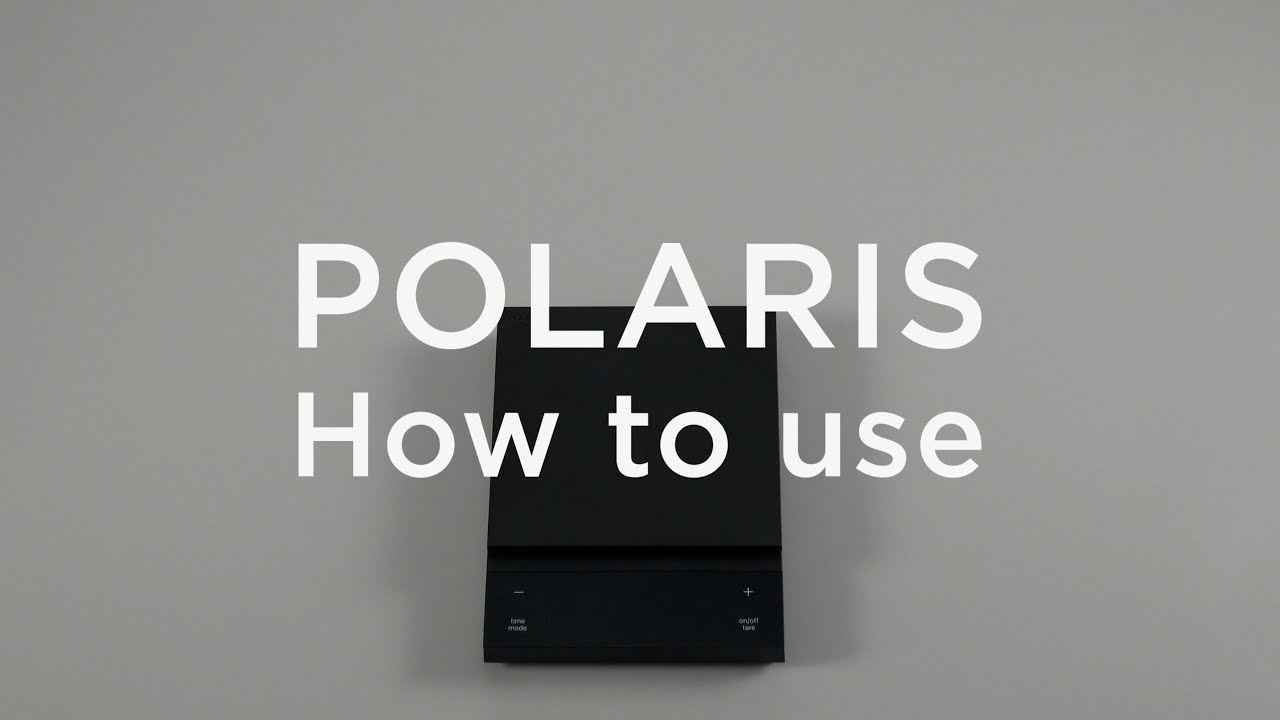
\includegraphics[width=0.48\linewidth]{pictures/youtube/2026/01/20260125_065246_youtube_001_4Ht3xvT-87k.jpg}
}
\end{center}




(２)抽出メソッド


ポラリス付属の説明書には粕谷哲氏監修による基本の抽出レシピが載っています。ポラリスなら経過時間も比率％も実時間で表示される訳ですから、ポラリスを使って、この通りのレシピで淹れてみたらどう？という意味ですね


0:00 に20％注ぐ（20\%の表示まで）

0:45 になったら、20％注ぐ（40％の表示まで）

1:30 になったら、20％注ぐ（60\%の表示まで）

2:15 になったら、20％注ぐ（80\%の表示まで）

2:45 になったら、20％注ぐ（100\%の表示まで）

3:30 になったら、ドリッパを外す


=====

「コーヒーの味わい方の調査」の目次はここ↓

\url{https://www.facebook.com/100002225117991/posts/25623563003967852/}



\paragraph{写真}
\begin{center}
\begin{minipage}{0.48\linewidth}
\centering
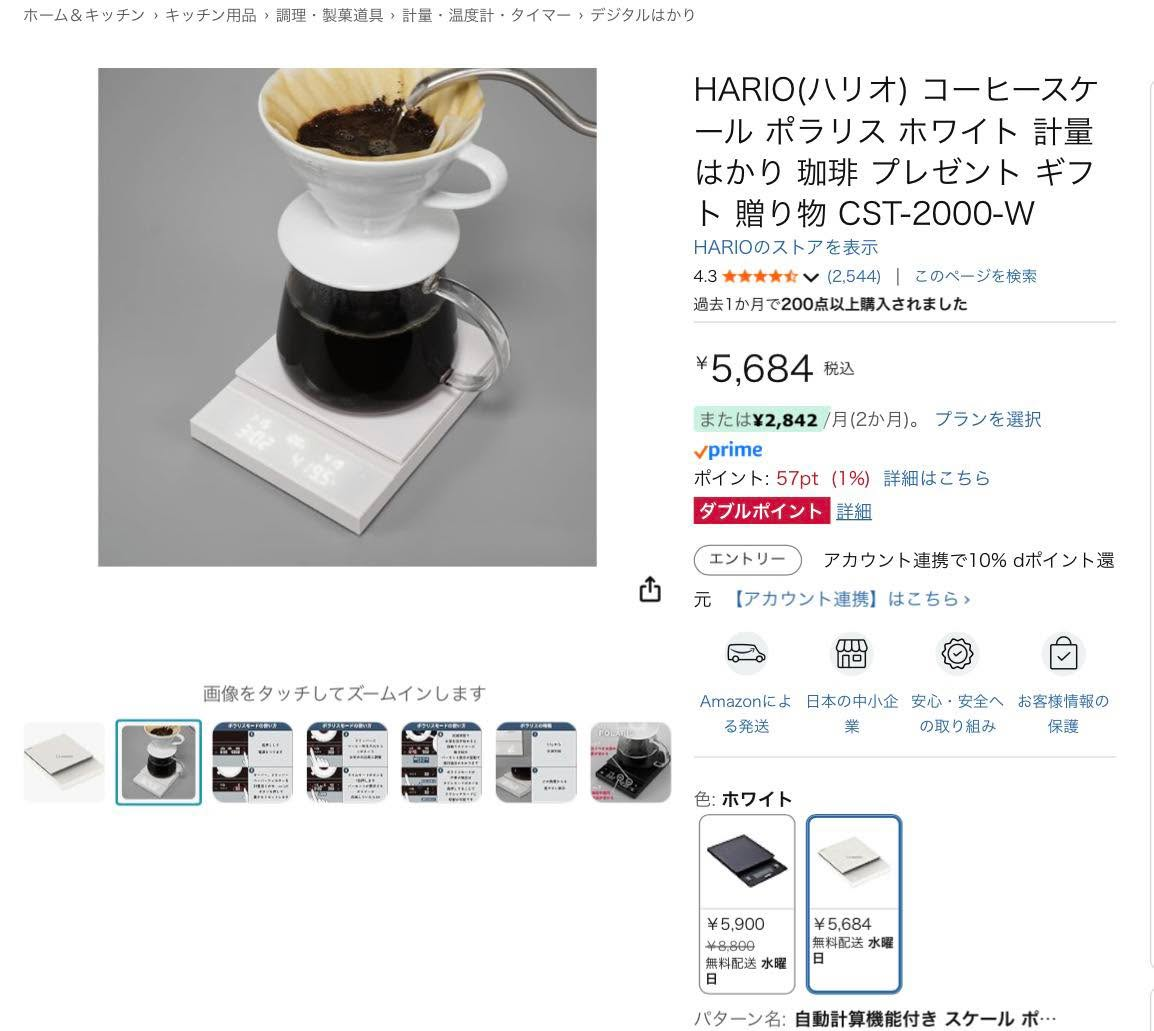
\includegraphics[width=\linewidth]{pictures/2026/01/20260125_065246_001.jpg}
\end{minipage}
\end{center}

\subsection*{2026年01月26日 13:03}
\addcontentsline{toc}{subsection}{2026年01月26日 13:03}

かなしい

山下和仁氏が亡くなられたとの情報が出ている

本当なのか

（Augustineオーガスチンはギター弦のブランド、おそらく信用できる情報なのだろう）


学生だった頃、展覧会の絵のギター編が出た

同じ世代だと思います（私の学生時代に氏は長崎大学の学生さんでしたから）

演奏会に行ったし、楽屋にも行った

当時、ギターの圧倒的な表現力にとても驚きましたし、大きなポテンシャルも感じました


\url{https://www.facebook.com/photo.php?fbid=1513187017482545&set=a.471515011649756&type=3}



\paragraph{写真}
\begin{center}
\begin{minipage}{0.48\linewidth}
\centering
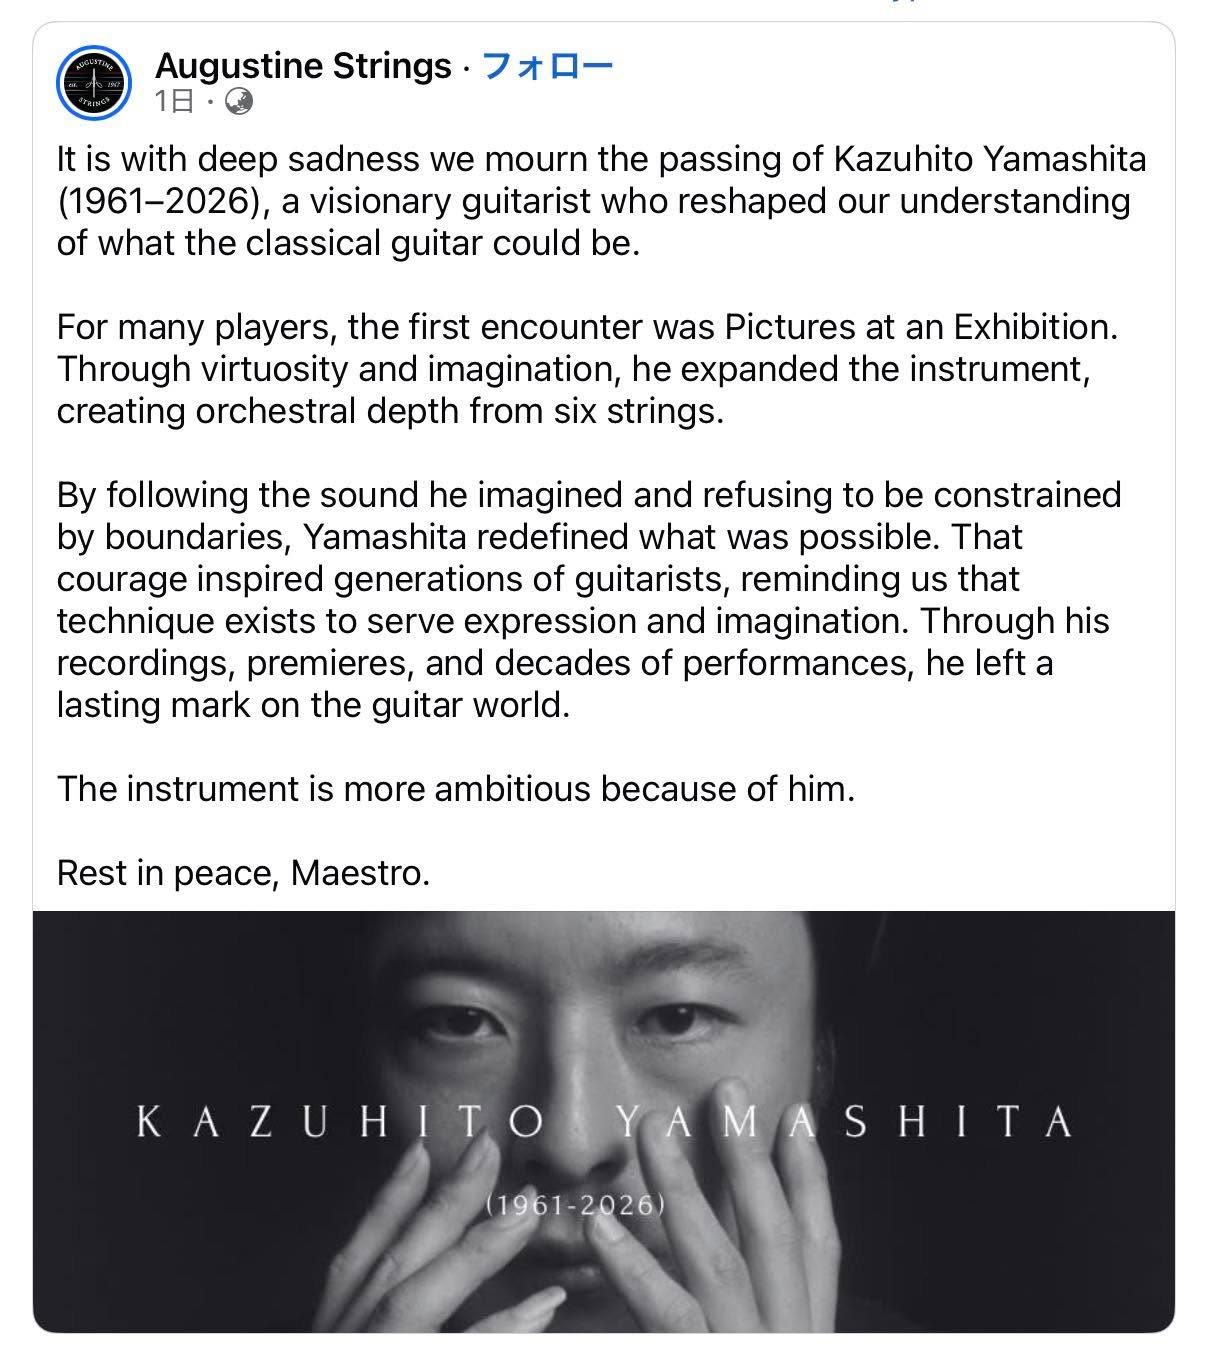
\includegraphics[width=\linewidth]{pictures/2026/01/20260126_130315_001.jpg}
\end{minipage}
\end{center}

\subsection*{2026年01月26日 22:44}
\addcontentsline{toc}{subsection}{2026年01月26日 22:44}

\paragraph{リンク}
\url{https://youtu.be/DjOQ69JjTRo}

\begin{center}
\href{https://youtu.be/DjOQ69JjTRo}{
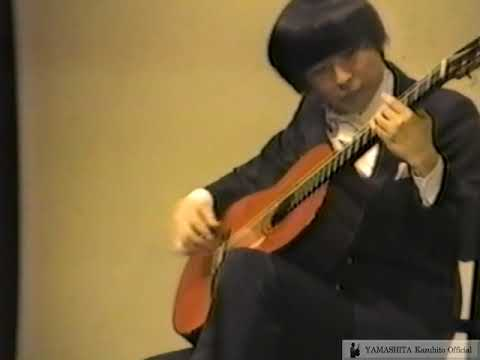
\includegraphics[width=0.48\linewidth]{pictures/youtube/2026/01/20260126_224445_youtube_001_DjOQ69JjTRo.jpg}
}
\end{center}

\subsection*{2026年01月27日 00:31}
\addcontentsline{toc}{subsection}{2026年01月27日 00:31}

今日は何て日なんでしょうか（山下和仁氏の訃報だけでなく）


日本が誇るリコーダ奏者であり、リコーダの研究製作の分野でもリードして来られた平尾（山岡）重治氏が亡くなられたとの事

（アンリュウ リコーダで行われた御講演を聞かせて頂いた事がありました）


お悔やみ申し上げます


\url{https://m.facebook.com/groups/189030912198717/permalink/1513238599777935/}



\subsection*{2026年01月27日 00:39}
\addcontentsline{toc}{subsection}{2026年01月27日 00:39}

\paragraph{リンク}
\url{https://youtu.be/IAo0GM4EWJc}

\begin{center}
\href{https://youtu.be/IAo0GM4EWJc}{
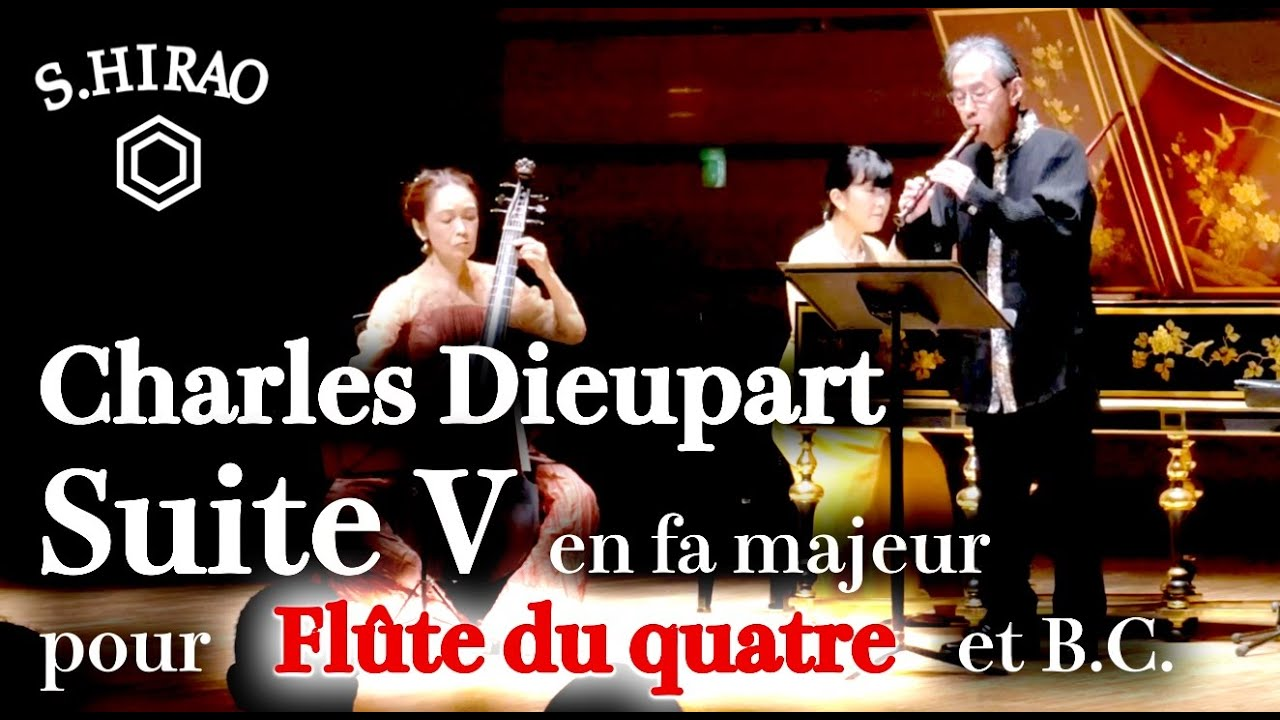
\includegraphics[width=0.48\linewidth]{pictures/youtube/2026/01/20260127_003957_youtube_001_IAo0GM4EWJc.jpg}
}
\end{center}

\subsection*{2026年01月27日 01:25}
\addcontentsline{toc}{subsection}{2026年01月27日 01:25}

\paragraph{リンク}
\url{https://youtu.be/y64BUIE_Z2Q}

\begin{center}
\href{https://youtu.be/y64BUIE_Z2Q}{
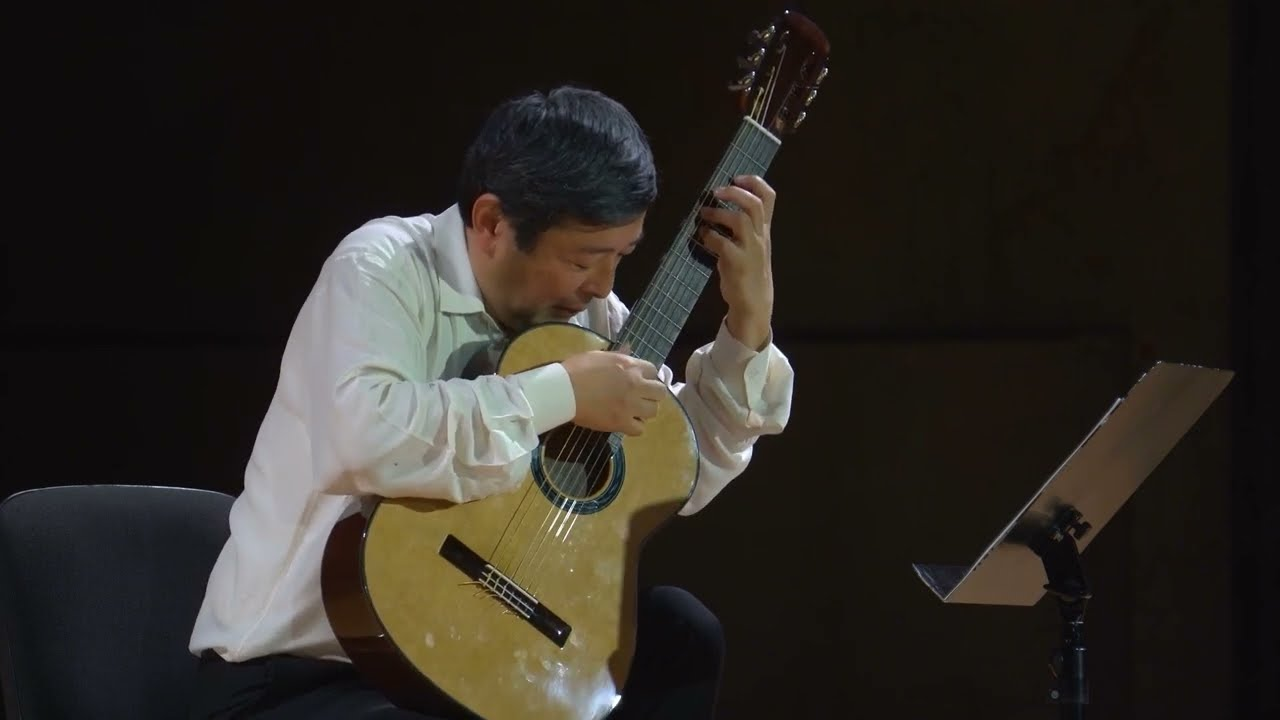
\includegraphics[width=0.48\linewidth]{pictures/youtube/2026/01/20260127_012556_youtube_001_y64BUIE_Z2Q.jpg}
}
\end{center}

\subsection*{2026年01月27日 06:30}
\addcontentsline{toc}{subsection}{2026年01月27日 06:30}

コーヒーの味についての個人的感想


コーヒー豆の味は、どの時点での味について論評されているものなのか

そもそも淹れたてのコーヒーは苦いが、味は時間の経過に従って急激に変化する

時間が経つと、苦みは減って飲みやすくなると共に、（どちらかと言えば）酸味が強く感じられる様になる

苦みが強い間は、その陰に酸味が隠れているため、感じられていないのかもしれません

更に時間が経つと、苦みも酸味も定常な状態に近づいている様な気がするから、その状態での味が、豆の特徴として論評されているものかと思います


モーニング コーヒーとして、近頃はコロンビアとエチオピアを日替わりで飲んでいます

エチオピアの方がどちらかと言えばマイルドだと感じますし、ひと口飲んだ後の味わいはコロンビアの方が長く残るような気がします

飲んだ後の味わいと言えば、夕方に飲むデカフェでは、飲んだ後あっという間に消えてしまい、直ぐに飲んだ気がしなくなります（そのため、ガブガブ2口3口と、いや２杯3杯と飲む事になってしまうのです）

ひと口飲んだ後の味というのは、カフェインの量を感じているのかもしれません


添付↓はUCCコーヒー アカデミーというYoutube（

\url{https://youtu.be/dPra-TVGqvU}

\begin{center}
\href{https://youtu.be/dPra-TVGqvU}{
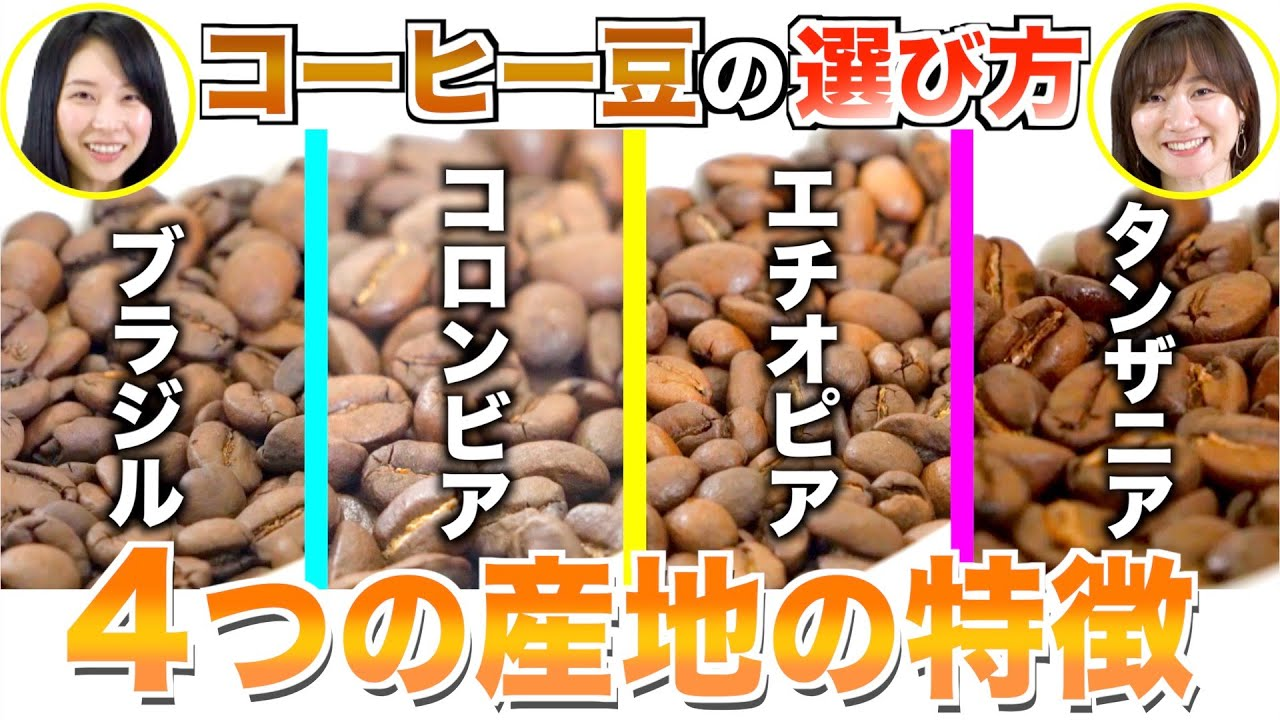
\includegraphics[width=0.48\linewidth]{pictures/youtube/2026/01/20260127_063028_youtube_001_dPra-TVGqvU.jpg}
}
\end{center}

）からの情報です


分かっていることをメモっておくと（言うまでもないかも、、）

深煎りに向かうほど苦くなり、浅煎りに向かうほど酸味が強く感じられる様なのですが、自分で煎る事はないので出会った豆の煎り方を受け入れているだけです

また、サイフォンの場合、ロートの中の状態（撹拌とか時間とか）によって、苦みなどは特に影響を受けやすいのは実感できる（サラッと降りてくると、お湯の状態に近づくけど、じっくり撹拌していると苦い）何杯分淹れるかによってもロートでの滞在時間は変えられるべきものなのだと思います（適切な値は各自の好み、実験的に求められるものでしょう）

更には、BrewRatio（粉：水）が1:12だとか1:13だとかと言う人がいる（YouTube）が、それは本当ですか？ミルにかけた時の粉の粒度、或いはそもそもの豆の種類にも依存するのかもしれませんが、私は1:15でも濃いのではないかという感覚でいます（参考になります 

\url{https://youtu.be/Tl97tMmyLX4}

\begin{center}
\href{https://youtu.be/Tl97tMmyLX4}{
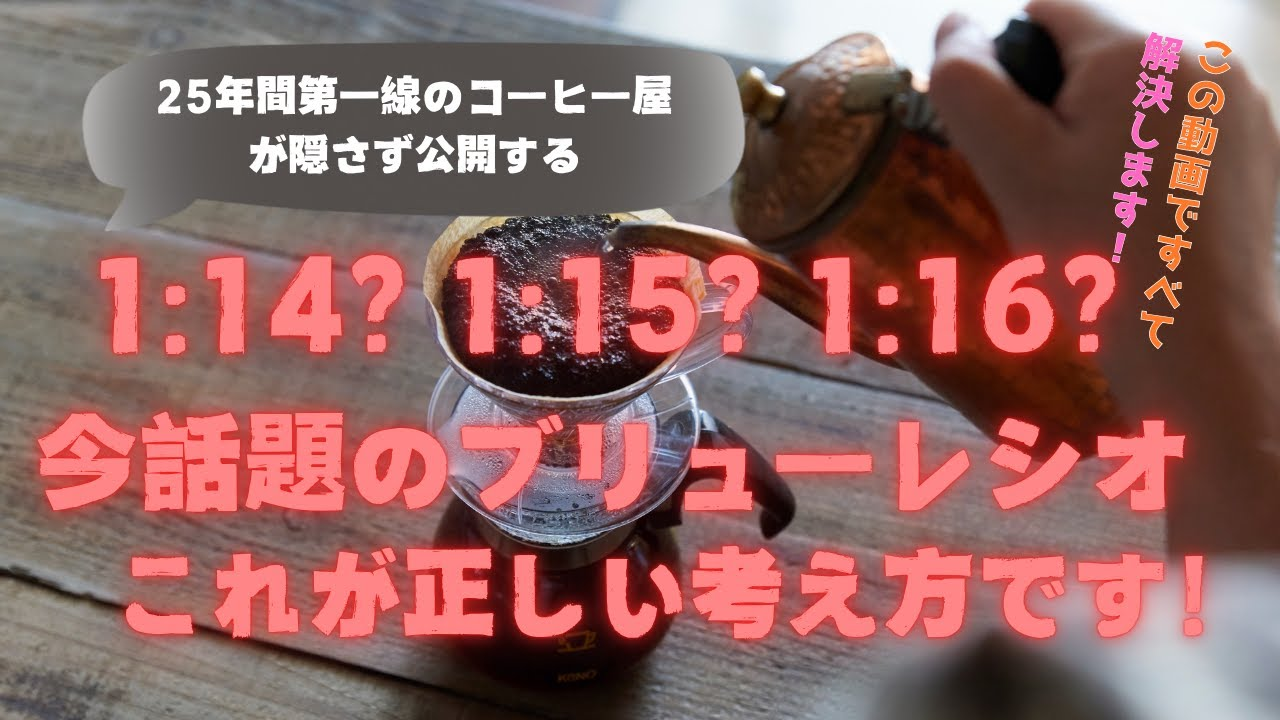
\includegraphics[width=0.48\linewidth]{pictures/youtube/2026/01/20260127_063028_youtube_002_Tl97tMmyLX4.jpg}
}
\end{center}

 ←私の感覚にかなり近い）

飲み慣れてくると、どんどん濃い味を志向する（豆の種類なら、添付の図の右下を目指していく）ものなのかもしれません


コーヒーの淹れ方について基本的には、各人の好みに合わせて実験的に、そして各個人ごとに求められていくものなのでしょうね（万人が納得する淹れ方などと言うものは、そもそも存在しないのだ）


=====

「コーヒーの味わい方の調査」の目次はここ↓

\url{https://www.facebook.com/100002225117991/posts/25623563003967852/}



\paragraph{写真}
\begin{center}
\begin{minipage}{0.48\linewidth}
\centering
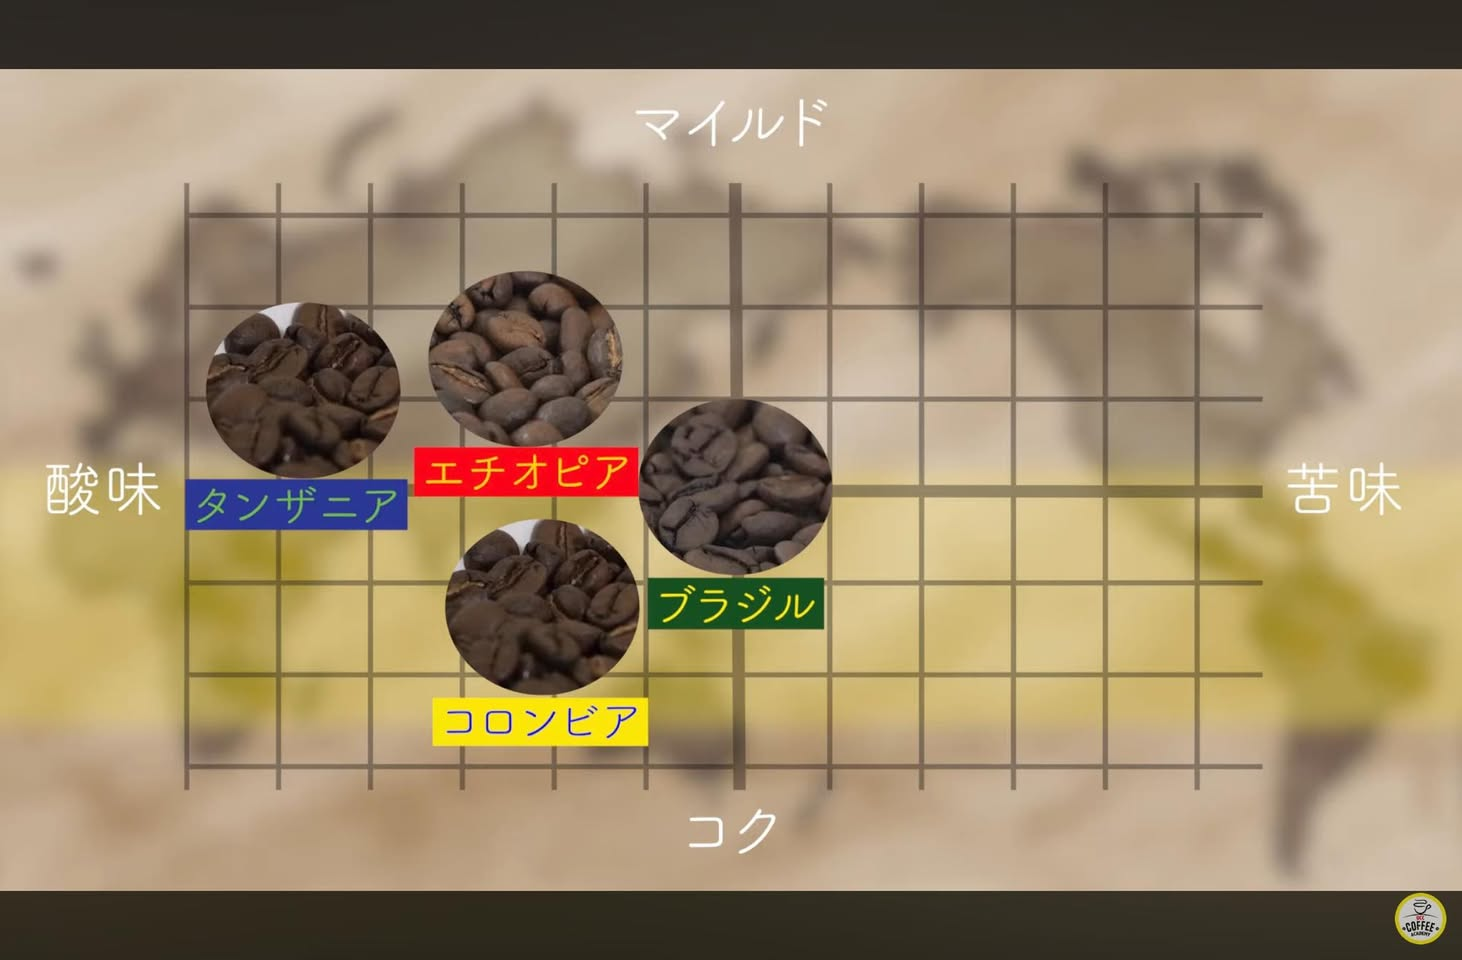
\includegraphics[width=\linewidth]{pictures/2026/01/20260127_063028_001.jpg}
\end{minipage}
\end{center}

\subsection*{2026年01月28日 22:52}
\addcontentsline{toc}{subsection}{2026年01月28日 22:52}

サイフォンによるコーヒー抽出

上の部分をロート、下をフラスコと言うらしい


水の加熱方法

(１)アルコールランプ（安価）

(２)ガスバーナー

(３)電熱器

(４)ハロゲンランプ（高価）


アルコール ランプで加熱するのが一般的ですが、アルコール ランプの場合、火力の調整ができない事もあって、ガスバーナーで代用されることもある様です

一方、そもそも部屋の中で炎を燃やしたくないというニーズもあるので、電熱器、ハロゲンランプ、遠赤外線による加熱などの方法が実用になってきている様です


ハロゲンランプは、得体の知れない複数のメーカーからの出品がAmazonにあって、サイフォン一式を含めていながら、それぞれ比較的安価に売られている様です。しかし火事の原因になったりすると怖いですし不安です

添付↓のBONMACのもの（BMBH-350N ）は、一旦UCC傘下の日本企業を経由して売られている様で信頼できる様な気がします（但し高価¥41,500になっているので購入対象からは除外）

もう一つ信頼出来ると思われる機種に、HARIOのBGSN2-350(¥44,000)がありますが、BONMACと似た様な金額になっています(業務用であり個人には売らないとの事なので自動的に除外)

また、BONMACとHARIOのハロゲンランプでは、サイフォンは別途購入する必要があります

一方、HARIOの電熱器のものは電熱器以外にフラスコ等サイフォン一式を揃えて付属しているのに安価（¥12,500）、私の様な初心者にとって手軽だと感じたので、こちらを手に入れる事にしました


リンク先（

\url{https://youtu.be/I97Vzdln1Sk}

\begin{center}
\href{https://youtu.be/I97Vzdln1Sk}{

\includegraphics[width=0.48\linewidth]{pictures/youtube/2026/01/20260128_225234_youtube_001_I97Vzdln1Sk.jpg}
}
\end{center}

）のコンペティション（Japan Siphonist Championship）の様子を何人か見ました

コンペでは、ハロンゲンランプにBONMACが使われている事、サイフォンにHARIOの2杯用TCAR-2（¥7,499）が使われている事が分ります

また、サイフォンでコーヒーを淹れる時の時間管理や、撹拌などのオペレーションについても、とても参考になりますし、何と言っても競技者の皆さんのプレゼンテーションが、色々な工夫もあって実に素晴らしいです


しかし、ちょっとだけ年寄りっぽい苦言を言うとするなら、後半のSignature Beverage（お店の看板料理）の説明では、コーヒー業界のtechnical terms なのか？カタカナ用語の連続で、コーヒーにaddictedな方にはpopular（と言うよりfamiliar ）なのかも知れませんが、私の様な田舎者には何を言ってるのか全く意味が分かりません（まあ、niceでsophisticatedなsomethingがavailable なんだ、とは伝わってきていますが）


カタカナ用語の連続に出会うと、それに合わせようとして、ルー大柴か長島⚪︎雄か、みたいな言い方になってしまいます


=====

「コーヒーの味わい方の調査」の目次はここ↓

\url{https://www.facebook.com/100002225117991/posts/25623563003967852/}



\paragraph{写真}
\begin{center}
\begin{minipage}{0.48\linewidth}
\centering
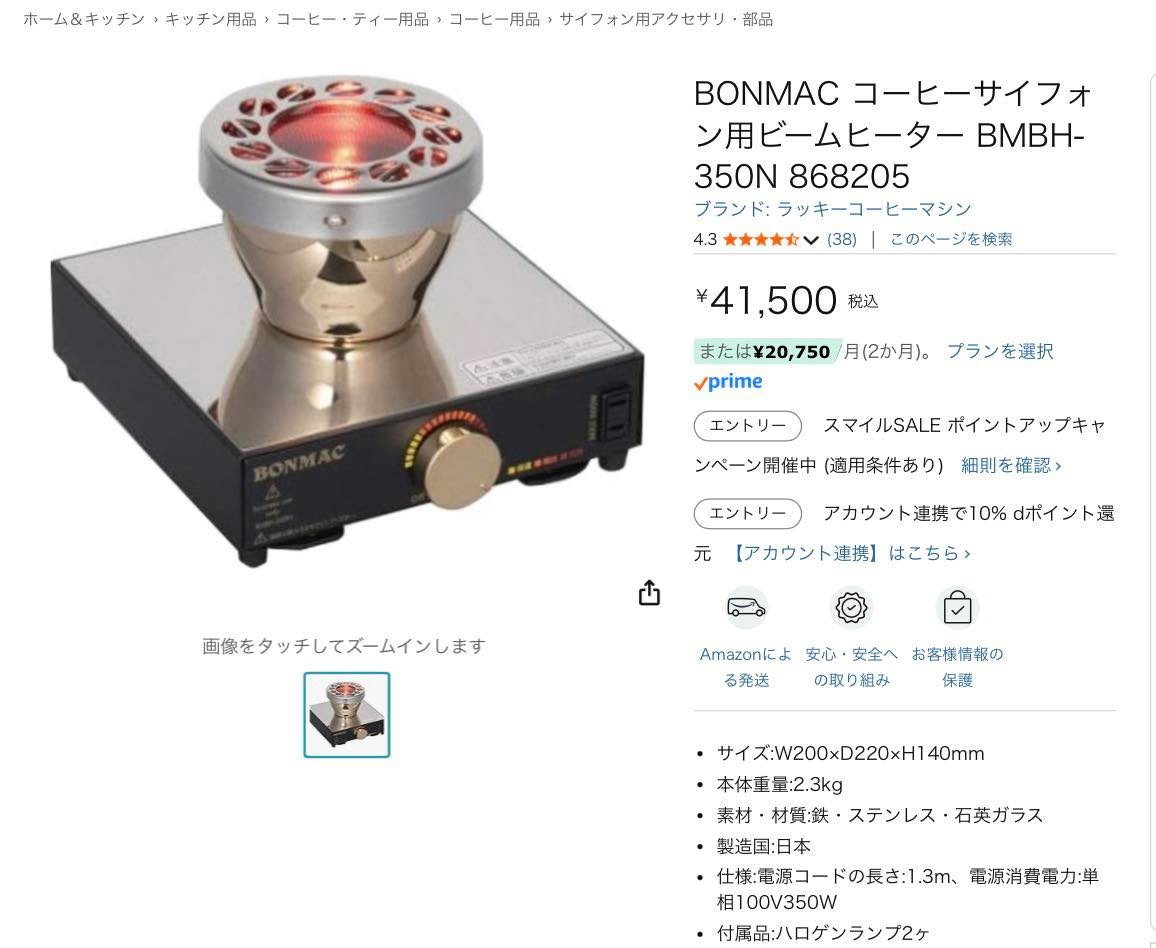
\includegraphics[width=\linewidth]{pictures/2026/01/20260128_225234_001.jpg}
\end{minipage}
\hfill
\begin{minipage}{0.48\linewidth}
\centering
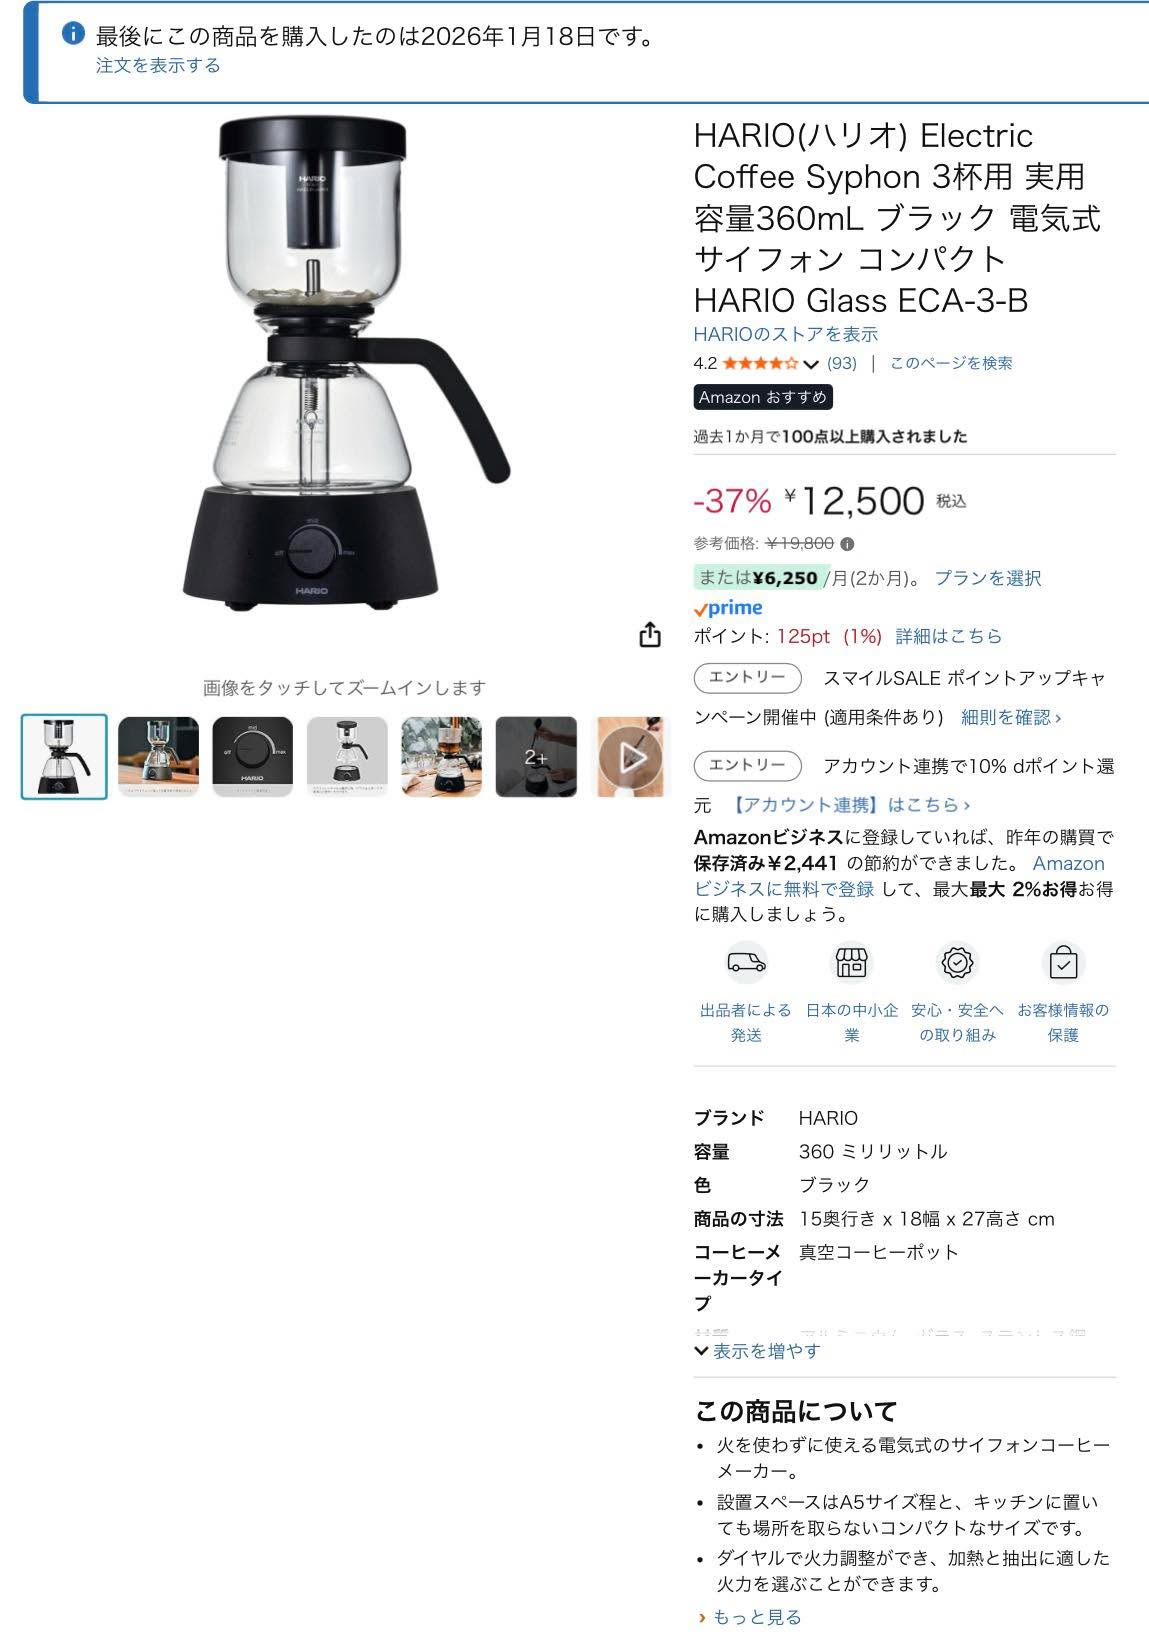
\includegraphics[width=\linewidth]{pictures/2026/01/20260128_225234_002.jpg}
\end{minipage}
\end{center}

\subsection*{2026年01月30日 00:45}
\addcontentsline{toc}{subsection}{2026年01月30日 00:45}

\paragraph{リンク}
\url{https://youtu.be/BdKvq6WlAgw}

\begin{center}
\href{https://youtu.be/BdKvq6WlAgw}{
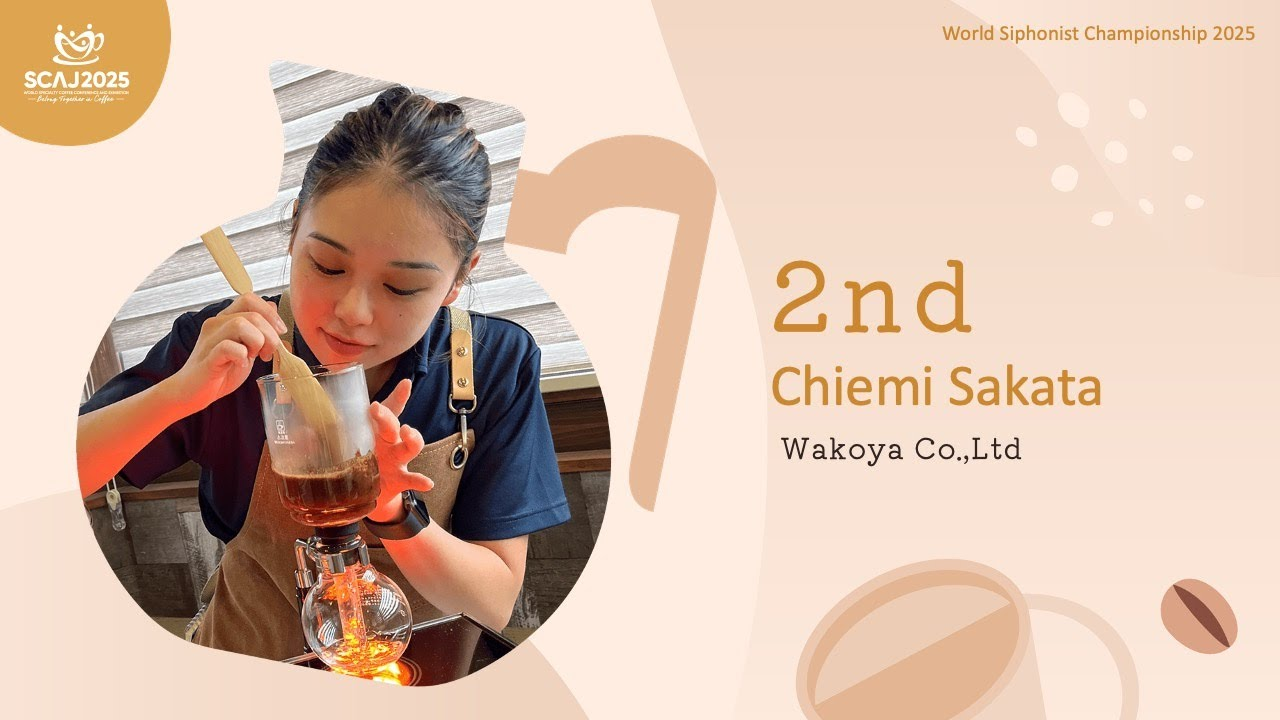
\includegraphics[width=0.48\linewidth]{pictures/youtube/2026/01/20260130_004554_youtube_001_BdKvq6WlAgw.jpg}
}
\end{center}

\section{2月}

\subsection*{2026年02月01日 01:06}
\addcontentsline{toc}{subsection}{2026年02月01日 01:06}

\paragraph{リンク}
\url{https://youtu.be/PxHFeQQmDsc}

\begin{center}
\href{https://youtu.be/PxHFeQQmDsc}{
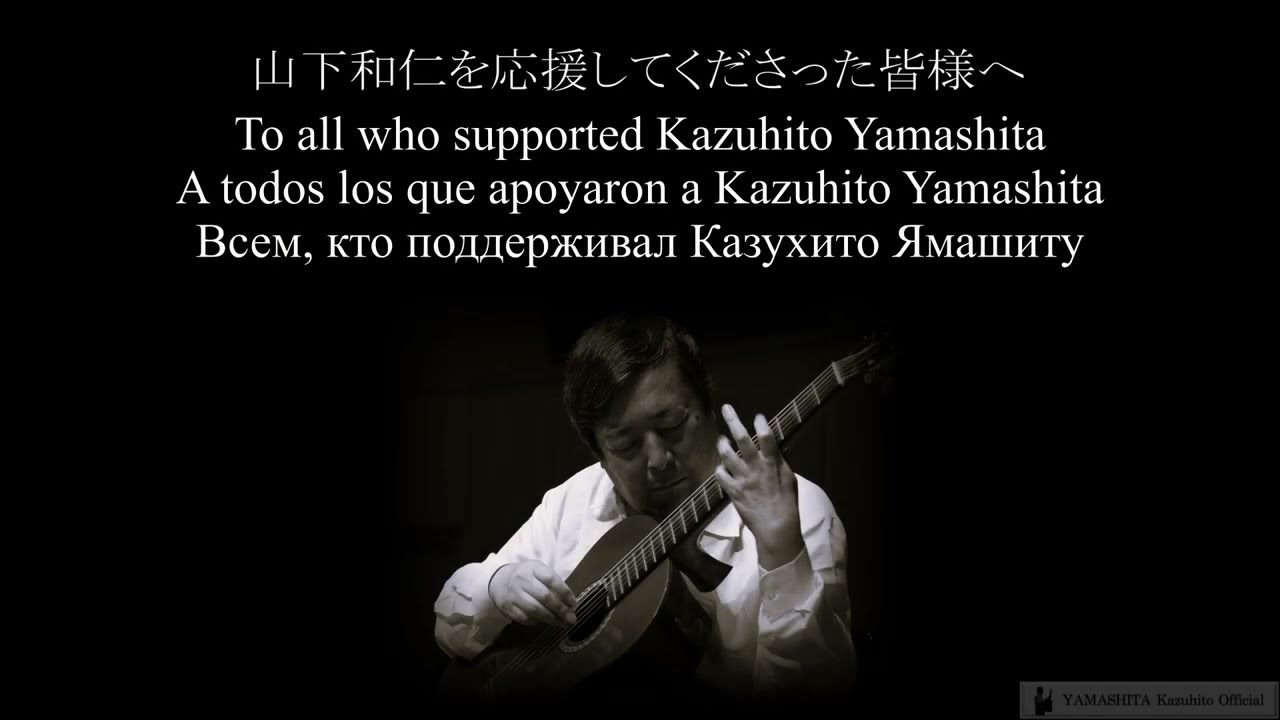
\includegraphics[width=0.48\linewidth]{pictures/youtube/2026/02/20260201_010603_youtube_001_PxHFeQQmDsc.jpg}
}
\end{center}

\subsection*{2026年02月01日 21:59}
\addcontentsline{toc}{subsection}{2026年02月01日 21:59}

これまで、この方の右手親指pの使い方に注目していました。親指の爪を使われる事もありますが、「親指の腹」を使って柔らかい音を出そうとしていらっしゃる様にも見えます。

更に、何と！「小指」でも弾いていらっしゃるんじゃないのか？今日になって気がつき（気になり）ました。私は右手の小指の爪は伸ばしていません。弦を弾くのにこれまで小指を使った事ありませんでしたから。（伸ばして、真似してみようかな）


\url{https://youtu.be/RwMd4p0MJ1A}

\begin{center}
\href{https://youtu.be/RwMd4p0MJ1A}{

\includegraphics[width=0.48\linewidth]{pictures/youtube/2026/02/20260201_215919_youtube_001_RwMd4p0MJ1A.jpg}
}
\end{center}




これまでバッハのPrelude, Fugue and Allegro（特にFugue）に挑戦してきているせいか、この曲の楽譜を見ると先ず「何て短い曲なんだ」と思ってしまいます。


（その後）

武満編の楽譜を（演奏してみようかと思って）眺めている。すると５個の音を重ねた和音が4カ所（この方の演奏では反復①を省略していらっしゃるので３カ所）に現れる。5本の弦を一緒に鳴らすには、p,i,m,a の４本の指では足りない。右手小指も使うとか、低いところの２本の弦をまとめてp指に担当させるなど、そういった事が必要になるということなのかな、という今の所の理解です。


（更にその後）

５個の音を重ねた和音ですが、（八部音符を8、四分音符を４と書く事にすると）888844という小節で、最後の４が５個の音の和音の場合に、その和音の１番低い音１個を最後の和音の装飾音のように少し先に出して弾いてしまって、続けて残りの４個を1つの和音の様にして弾く（← pが低音弦２本を弾いているのと同じ事か?）という「（荒）技」が使われている事が分っちゃいました（他の方はどうやって演奏していらっしゃるだろうか←案外音を１個省略してたり、、、してないか？）


====

この記事は、以下↓の記事の続きです

\url{https://www.facebook.com/100002225117991/posts/24495919103398920/}



\subsection*{2026年02月01日 23:00}
\addcontentsline{toc}{subsection}{2026年02月01日 23:00}

\paragraph{リンク}
\url{https://youtu.be/kZpv5Qqipco}

\begin{center}
\href{https://youtu.be/kZpv5Qqipco}{
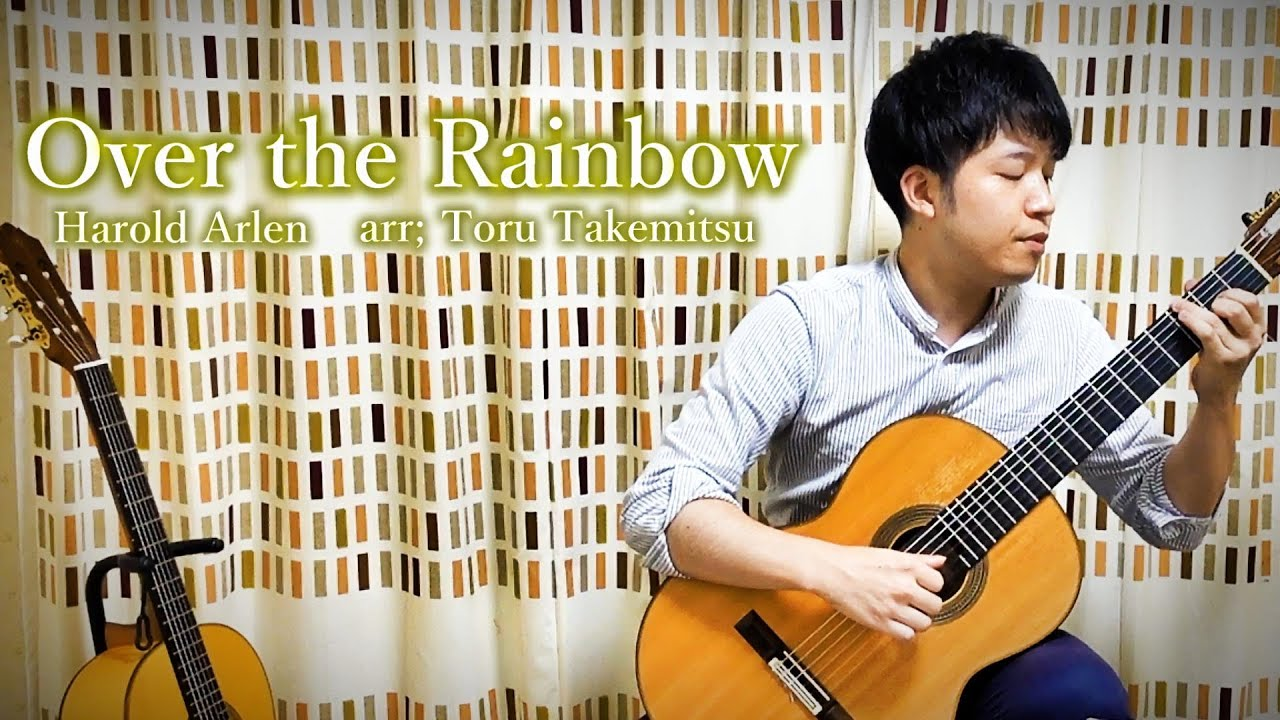
\includegraphics[width=0.48\linewidth]{pictures/youtube/2026/02/20260201_230018_youtube_001_kZpv5Qqipco.jpg}
}
\end{center}

\subsection*{2026年02月01日 23:01}
\addcontentsline{toc}{subsection}{2026年02月01日 23:01}

\paragraph{リンク}
\url{https://youtu.be/3lD-WLesNao}

\begin{center}
\href{https://youtu.be/3lD-WLesNao}{
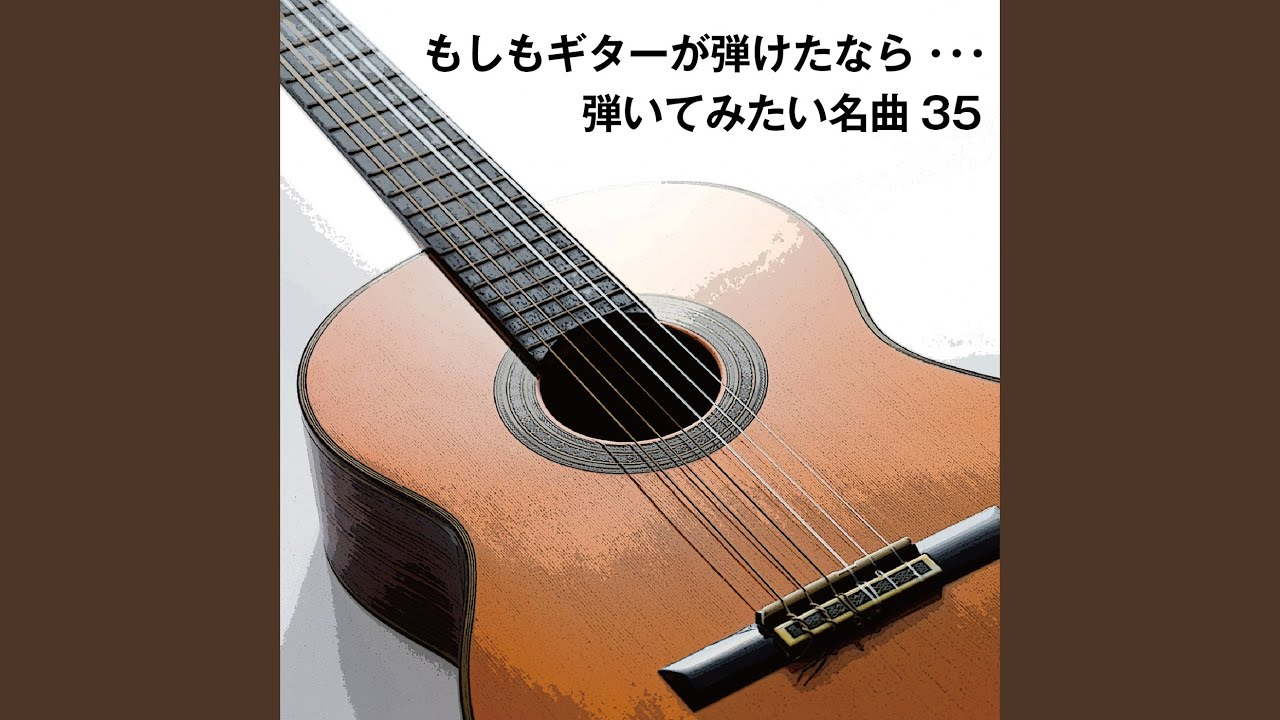
\includegraphics[width=0.48\linewidth]{pictures/youtube/2026/02/20260201_230100_youtube_001_3lD-WLesNao.jpg}
}
\end{center}

\subsection*{2026年02月02日 00:00}
\addcontentsline{toc}{subsection}{2026年02月02日 00:00}

\paragraph{リンク}
\url{https://youtu.be/gGWENHM5Q2M}

\begin{center}
\href{https://youtu.be/gGWENHM5Q2M}{
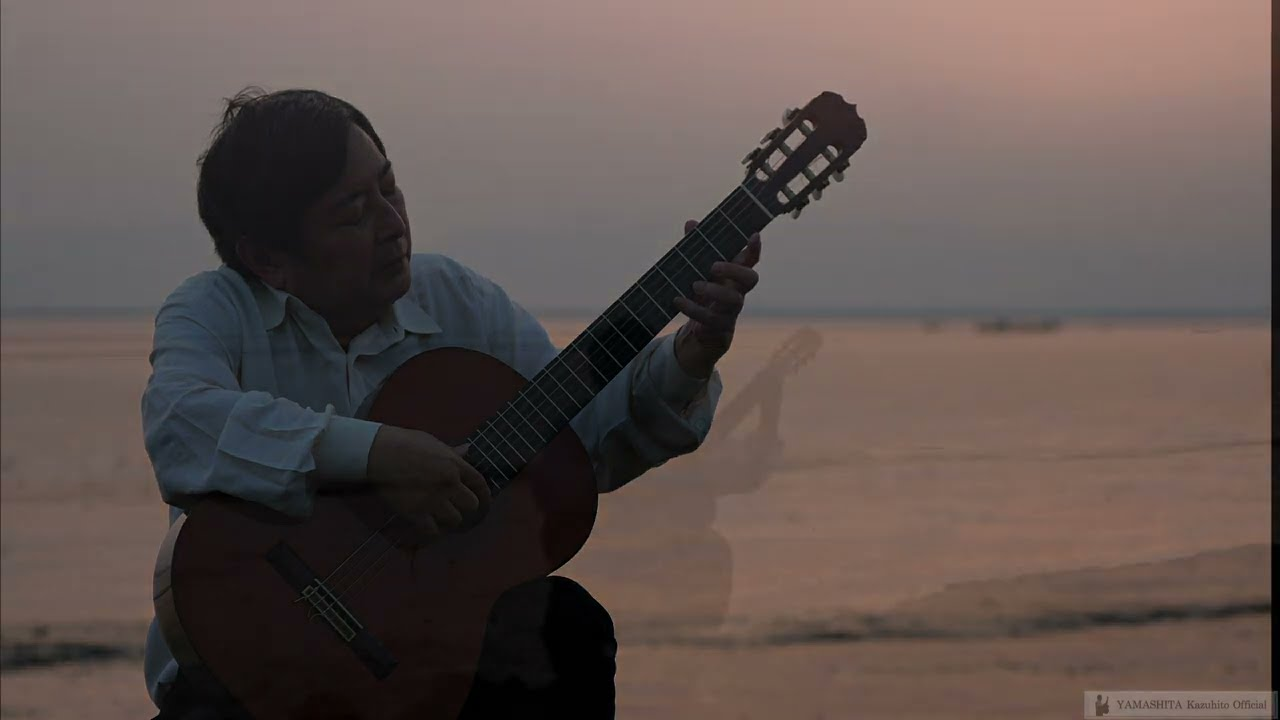
\includegraphics[width=0.48\linewidth]{pictures/youtube/2026/02/20260202_000005_youtube_001_gGWENHM5Q2M.jpg}
}
\end{center}

\subsection*{2026年02月02日 01:05}
\addcontentsline{toc}{subsection}{2026年02月02日 01:05}

\paragraph{リンク}
\url{https://youtu.be/joopZ1R-ZlU}

\begin{center}
\href{https://youtu.be/joopZ1R-ZlU}{
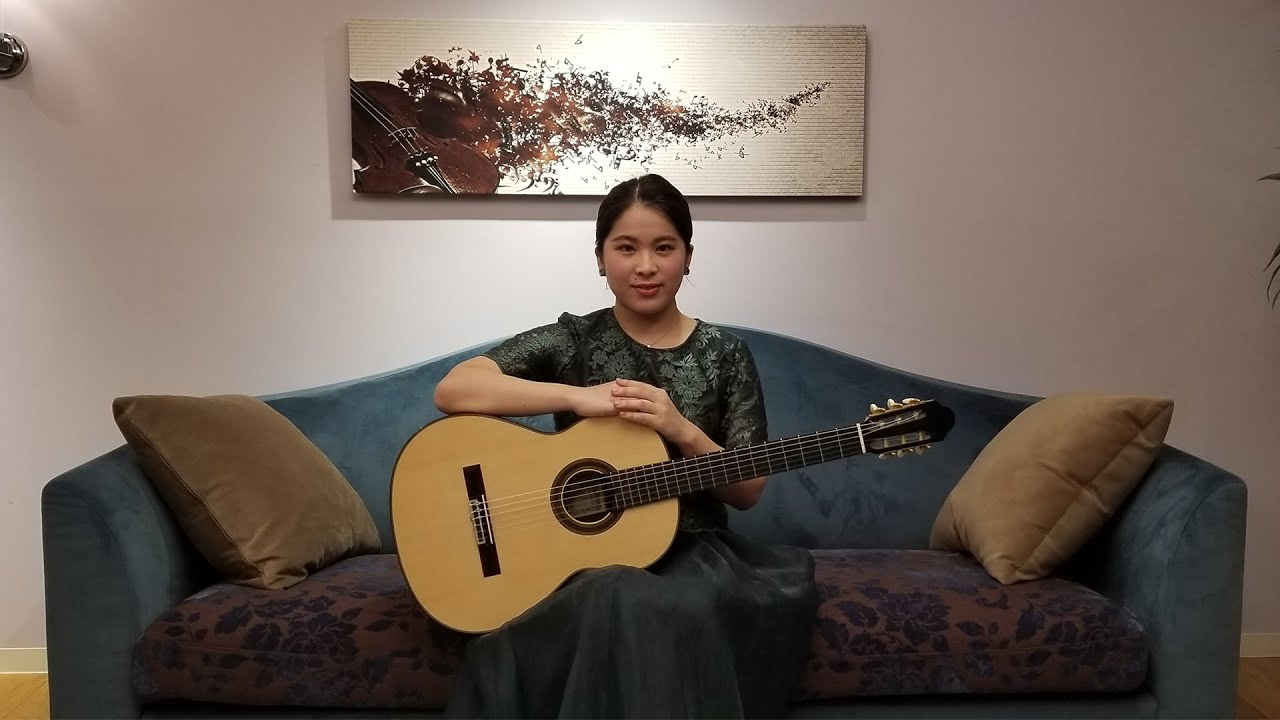
\includegraphics[width=0.48\linewidth]{pictures/youtube/2026/02/20260202_010530_youtube_001_joopZ1R-ZlU.jpg}
}
\end{center}

\subsection*{2026年02月02日 09:53}
\addcontentsline{toc}{subsection}{2026年02月02日 09:53}

ここしばらく、Prelude, Fugue and Allegro（BWV998） のFugueを一通り通して弾く事を日課に課して（？）きている。それにしても、このFugueはホンマに「長い！」曲だ。本当なら難しい運指の箇所（下↓の4カ所ほど）を集中的に練習する必要があるという自覚、持ってはいるのですが、、、一回通しでならしたらもう、お腹いっぱいで、更に練習する様なエネルギー（気力？）が残っていない。


第1の難所：35〜40小節

第2の難所：47〜49小節

第3の難所：55〜62小節 ← (55,56)+(57,58)+(59,60)+(61,62）

第4の難所：71〜75小節


これ以外にも、こまごまとした部分部分に指の回らない所はあるんだけど、、、


この方もお上手です（羨ましいよ←真似して少しでも近づきたい）

\url{https://youtu.be/rwEzi6MtUMI}

\begin{center}
\href{https://youtu.be/rwEzi6MtUMI}{
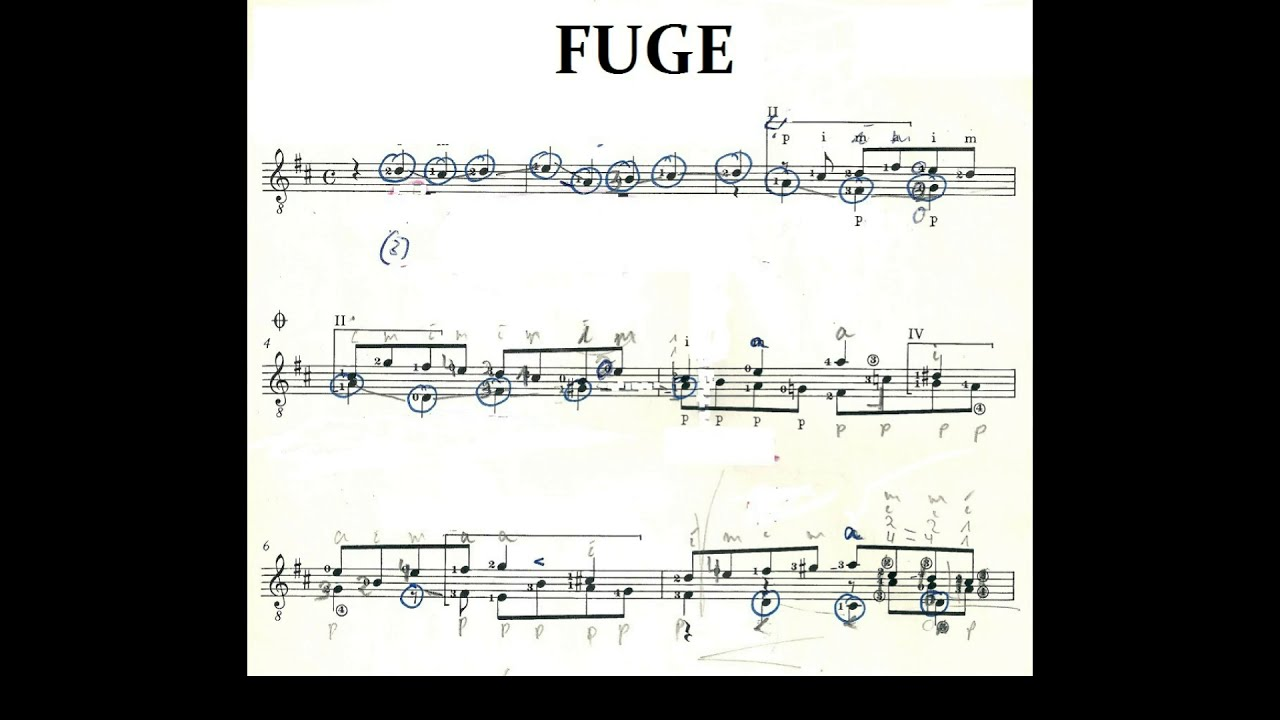
\includegraphics[width=0.48\linewidth]{pictures/youtube/2026/02/20260202_095322_youtube_001_rwEzi6MtUMI.jpg}
}
\end{center}



（75小節目はトリル無しでもいいんだね←Segovia編でも無しだった）

（この楽譜は誰編なんだろう？←おっと、Transcription for  Guitar by Heinz Teuchert. との記述がある）


===

この記事は、ここ↓の記事の続きです

\url{https://m.facebook.com/story.php?story_fbid=25562657750058378&id=100002225117991}



\subsection*{2026年02月03日 01:37}
\addcontentsline{toc}{subsection}{2026年02月03日 01:37}

\paragraph{リンク}
\url{https://youtu.be/rwEzi6MtUMI}

\begin{center}
\href{https://youtu.be/rwEzi6MtUMI}{
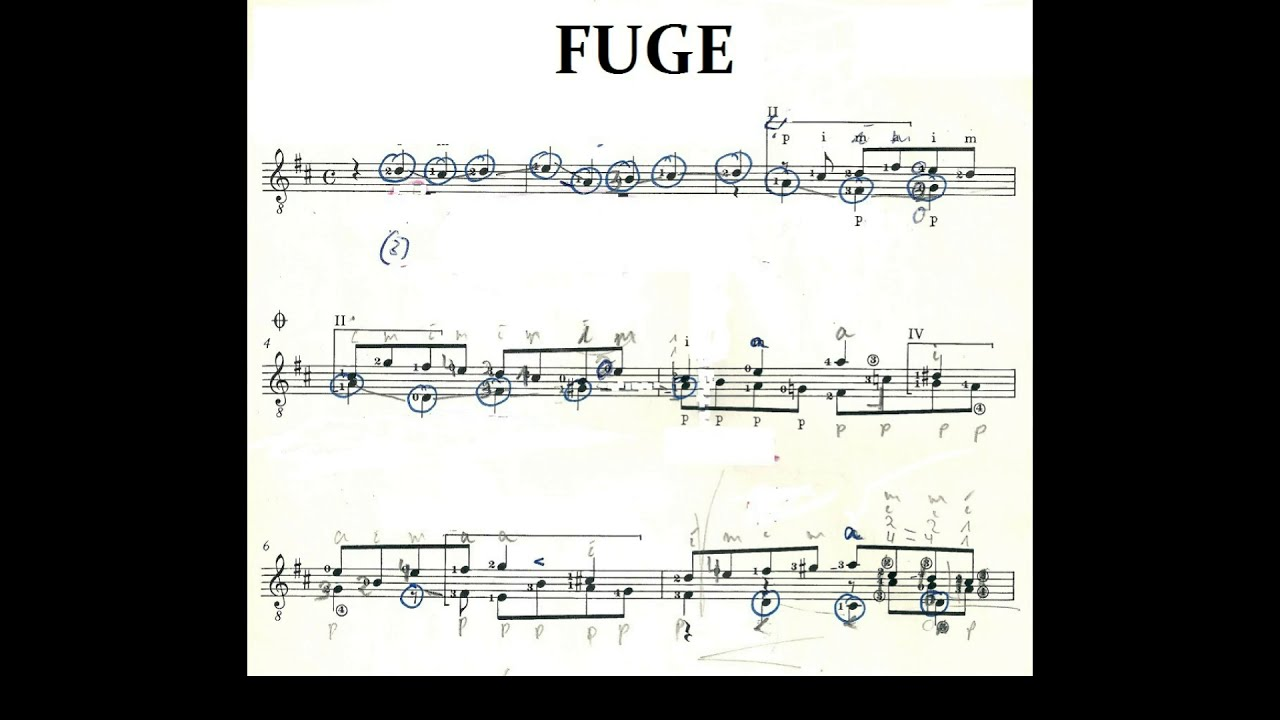
\includegraphics[width=0.48\linewidth]{pictures/youtube/2026/02/20260203_013713_youtube_001_rwEzi6MtUMI.jpg}
}
\end{center}

\subsection*{2026年02月04日 09:05}
\addcontentsline{toc}{subsection}{2026年02月04日 09:05}

練習中のPrelude, Fugue and Allegro（BWV998） のFugueについて


この方の演奏

\url{https://youtu.be/yGvJz3UQA0s?t=193}

\begin{center}
\href{https://youtu.be/yGvJz3UQA0s?t=193}{
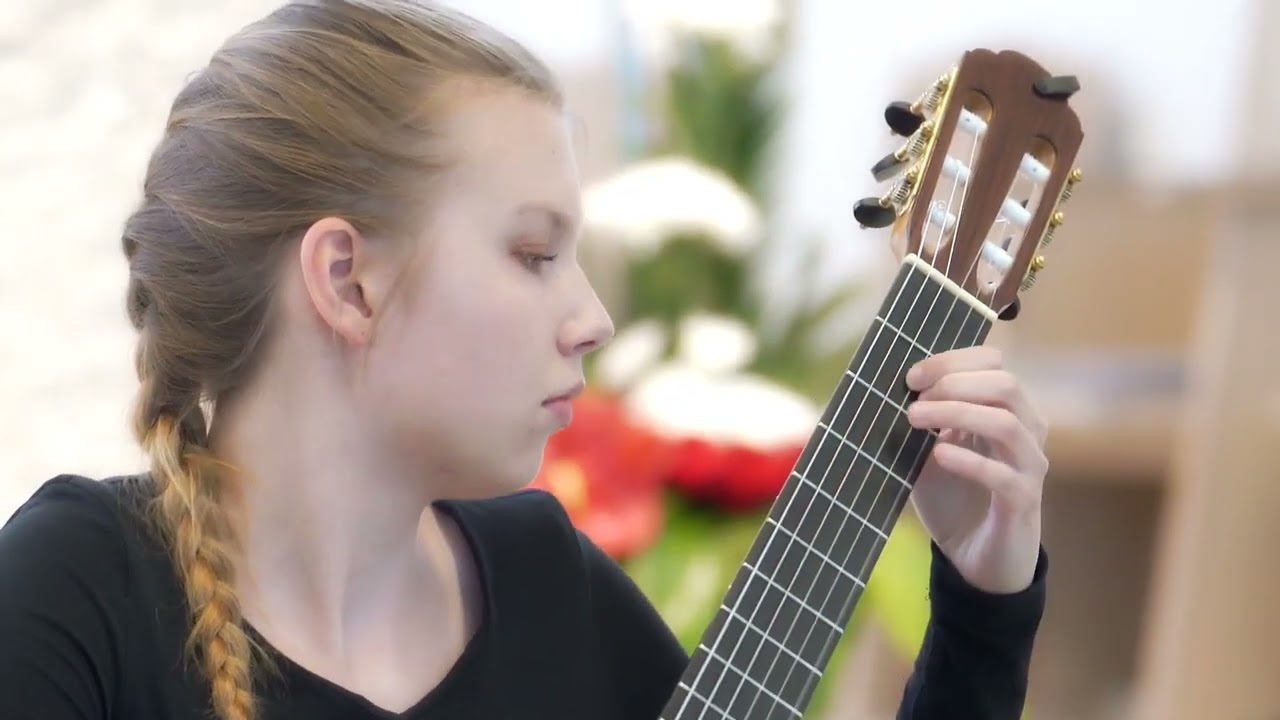
\includegraphics[width=0.48\linewidth]{pictures/youtube/2026/02/20260204_090510_youtube_001_yGvJz3UQA0s.jpg}
}
\end{center}



や、この方の演奏

\url{https://youtu.be/UGQFnJDCRls}

\begin{center}
\href{https://youtu.be/UGQFnJDCRls}{
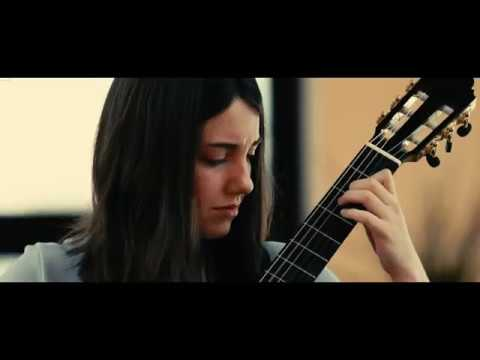
\includegraphics[width=0.48\linewidth]{pictures/youtube/2026/02/20260204_090510_youtube_002_UGQFnJDCRls.jpg}
}
\end{center}



や、この方の演奏

\url{https://youtu.be/80n4D_QOzUk?t=204}

\begin{center}
\href{https://youtu.be/80n4D_QOzUk?t=204}{
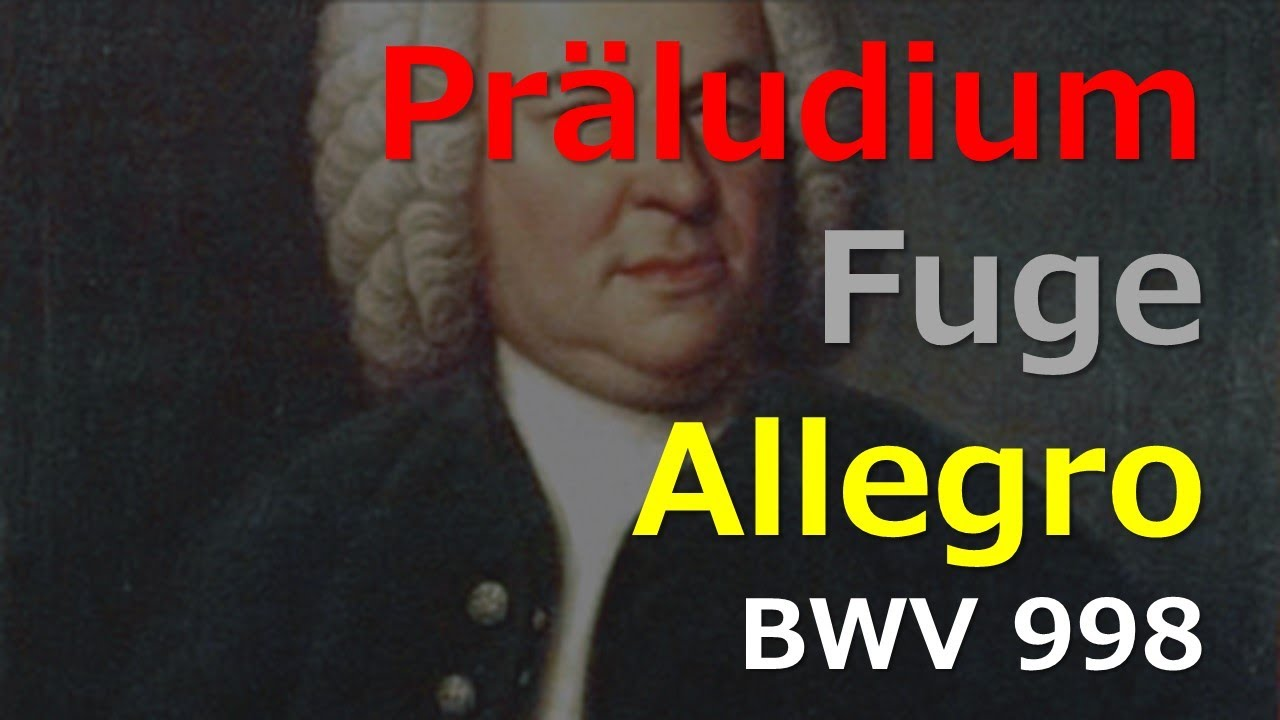
\includegraphics[width=0.48\linewidth]{pictures/youtube/2026/02/20260204_090510_youtube_003_80n4D_QOzUk.jpg}
}
\end{center}



を見て（聞いて)いると、どうも私の見ているKarl Scheit （シャイト）編の楽譜とは色々と違っている様な気がしていました。（益田正洋氏の演奏については演奏者自身によるアレンジもあるとは思います）


そこで、手元にあったもう一つの編曲譜Segovia編を一通り見直してみる事にしました。そもそもSegovia編の楽譜には、ディナーミク、アゴーギク、その他表情記号も記載されているので、いずれ真面目に見てみたいと思っていました（ただ、今回特に注目するのは運指です）。因みにScheit編の楽譜に表情記号等の類いは一切書かれていません。私の印象では、Segovia編はSegovia氏ご本人の浪漫ティックな嗜好による表情づけを露骨に反映した「作譜」がなされているのに対して、Scheit編では原典の楽譜にある音符をできるだけ編曲譜に再現させようとするストイックな「移行楽譜」を目指したもの、という感じがしています。


さて運指ですが、分散和音に入る前までを弾いてみた所では、どうもSegovia編の方が重ねている音が少ない所があるみたいです。でも、その分「主題になっている音の動き」をよく聞かせている様に感じます。また、運指も比較的合理的だと思われる箇所が散見される様な気もします。

但し、私が演奏する上で更なる「難所」と感じている所は、分散和音に入ってから現れるので（下↓のリンク先参照）、、、（Segovia編の運指がScheit編よりも容易になる事を期待しているのですが）→結局弾き易い方の運指を選ぶ事にすると思います。


（その後）

分散和音以降も弾いてみました。Segovia編の方がローポジション（と言うのか低い音域の弦）を使う運指になっていて、音は高音域での運指を使うScheit編よりも大きく明るく響く印象はありました。ただ、既にScheit編で「演奏上の難所」の攻略を始めてしまっていたためでしょうか？今のままの運指でいいや、と言う気になっています。


===

この記事は、ここ↓の記事の続きです

（Fugue「演奏上の難所」については以下↓に）

\url{https://www.facebook.com/100002225117991/posts/25697875713203247/}



\subsection*{2026年02月04日 17:51}
\addcontentsline{toc}{subsection}{2026年02月04日 17:51}

\paragraph{リンク}
\url{https://youtu.be/pTkE1_pClUs}

\begin{center}
\href{https://youtu.be/pTkE1_pClUs}{
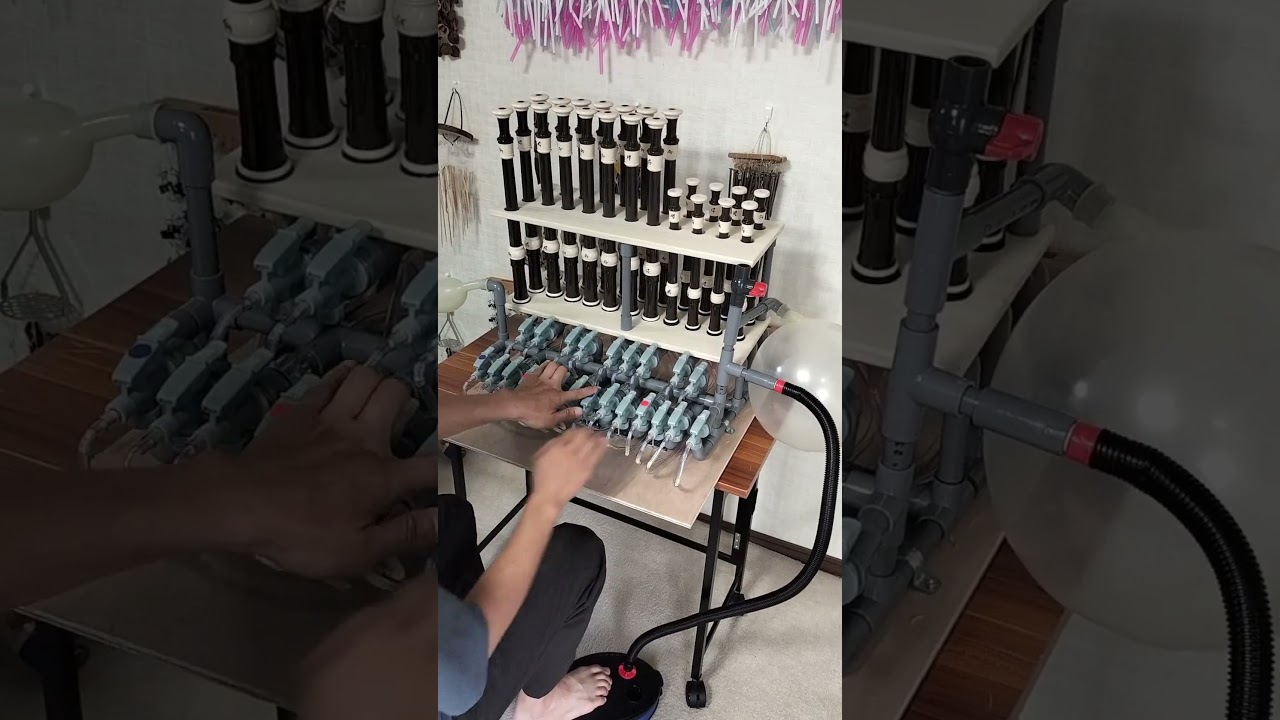
\includegraphics[width=0.48\linewidth]{pictures/youtube/2026/02/20260204_175150_youtube_001_pTkE1_pClUs.jpg}
}
\end{center}

\subsection*{2026年02月04日 17:54}
\addcontentsline{toc}{subsection}{2026年02月04日 17:54}

\paragraph{リンク}
\url{https://youtu.be/cG3VHvKCDzQ}

\begin{center}
\href{https://youtu.be/cG3VHvKCDzQ}{
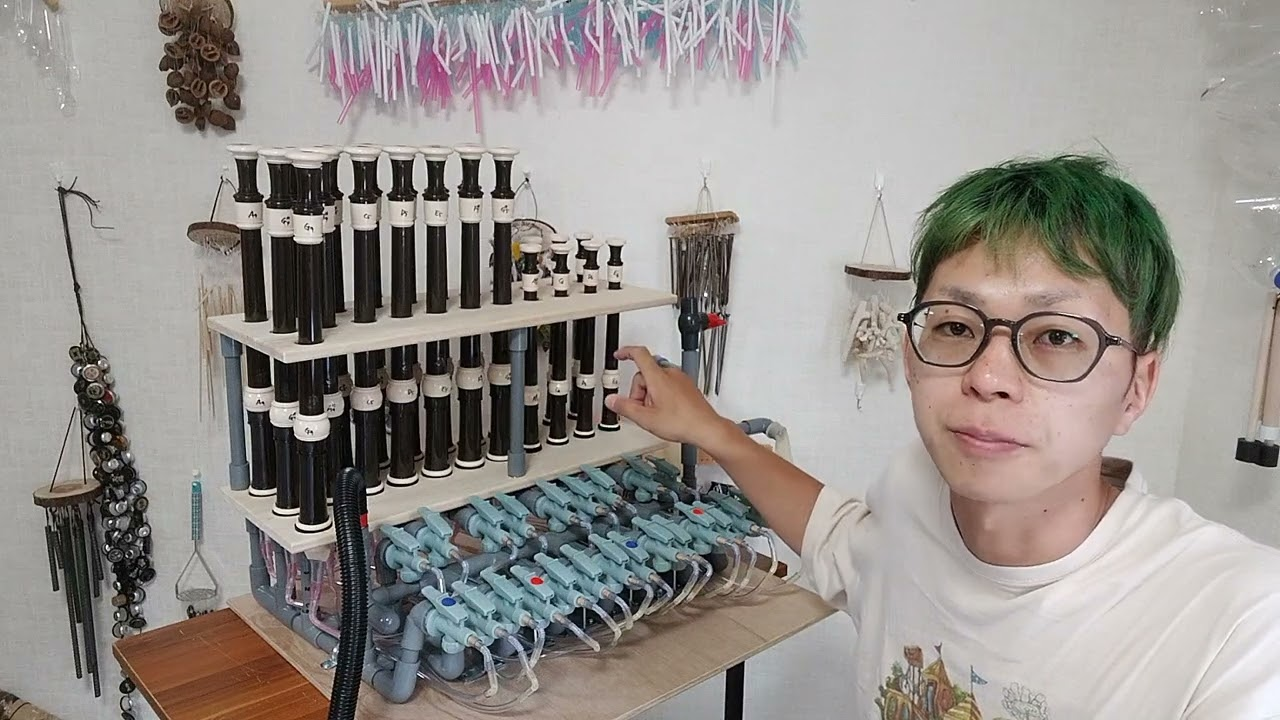
\includegraphics[width=0.48\linewidth]{pictures/youtube/2026/02/20260204_175428_youtube_001_cG3VHvKCDzQ.jpg}
}
\end{center}

\subsection*{2026年02月05日 15:49}
\addcontentsline{toc}{subsection}{2026年02月05日 15:49}

2月5日の兼六園の梅です。咲いている木は4〜5本くらいかな。

未だ大部分の木は蕾ばっかりの状態だから、これからどんどん咲いてくるのではないかと思われます。

（園内の除雪、お疲れ様です）


===

この記事は、以下↓の記事の続きです

\url{https://m.facebook.com/story.php?story_fbid=25534784719512348&id=100002225117991}



\paragraph{写真}
\begin{center}
\begin{minipage}{0.48\linewidth}
\centering
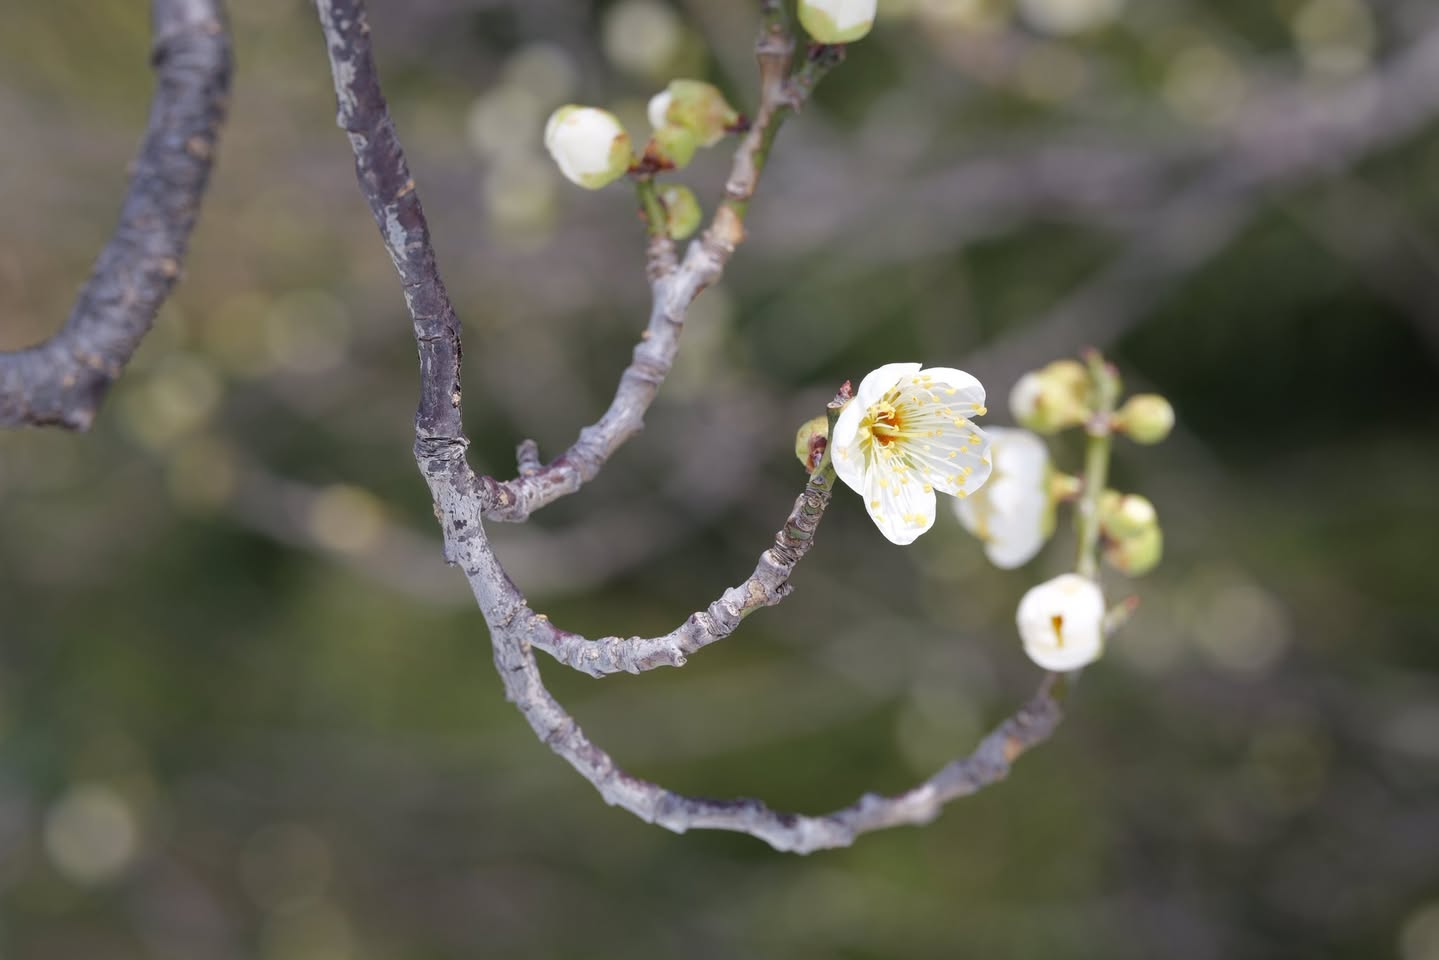
\includegraphics[width=\linewidth]{pictures/2026/02/20260205_154932_001.jpg}
\end{minipage}
\hfill
\begin{minipage}{0.48\linewidth}
\centering
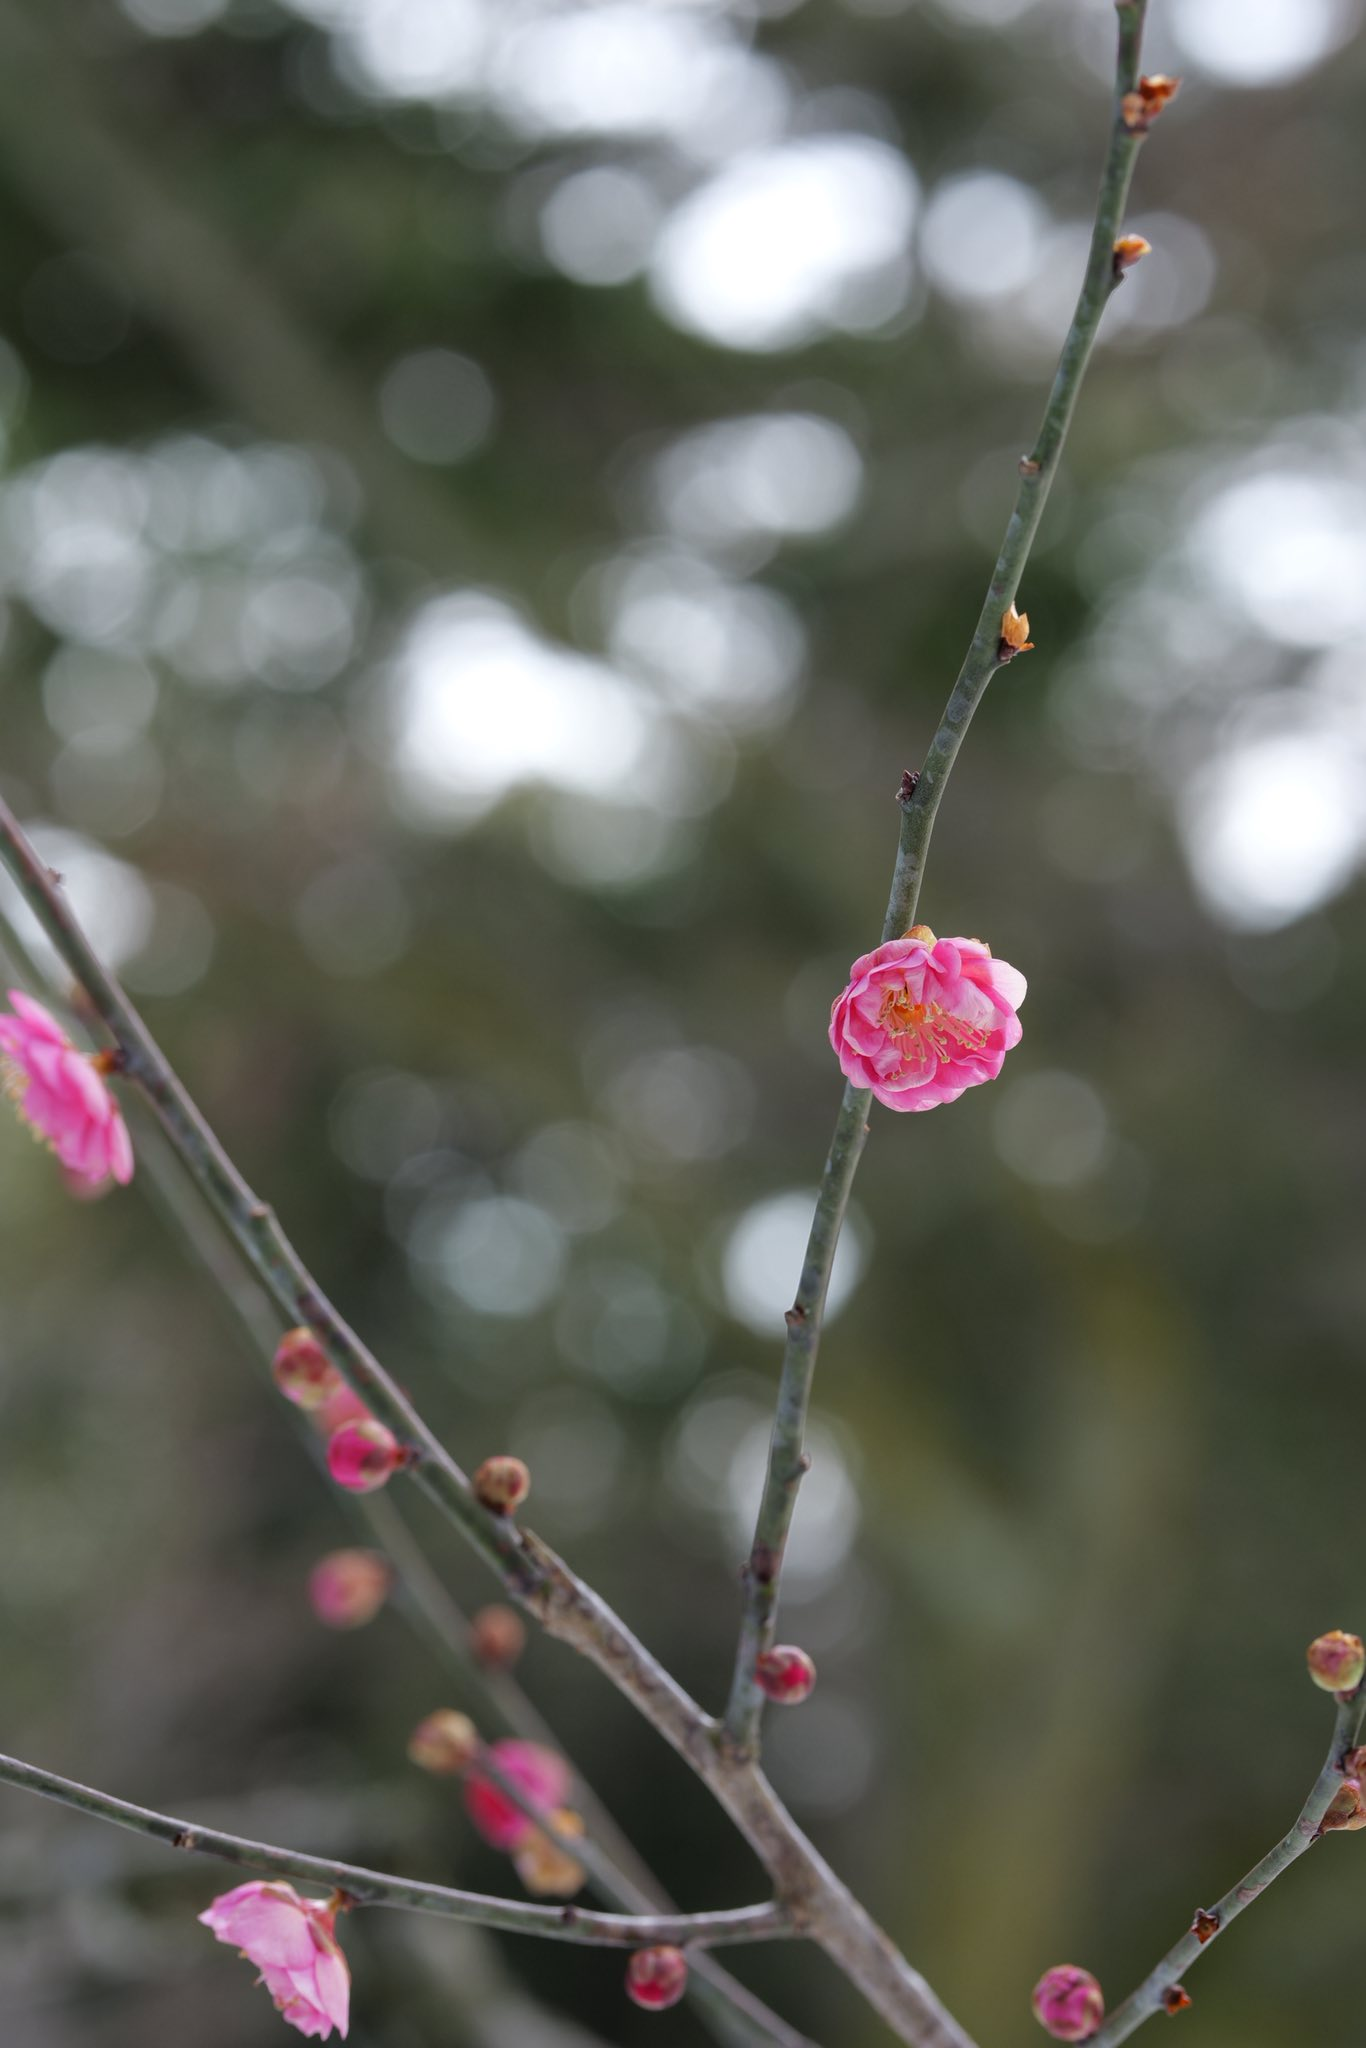
\includegraphics[width=\linewidth]{pictures/2026/02/20260205_154932_002.jpg}
\end{minipage}
\end{center}

\subsection*{2026年02月05日 23:32}
\addcontentsline{toc}{subsection}{2026年02月05日 23:32}

マタイ受難曲（BWV244）より（＝54番コラール）

これは受難曲全体を通して何度も繰り返し流れているあの主題かな？


演奏は岡本拓也氏

氏の演奏は優しさに溢れて心が洗われるようです

\url{https://youtu.be/gasmVmlGAeA}

\begin{center}
\href{https://youtu.be/gasmVmlGAeA}{
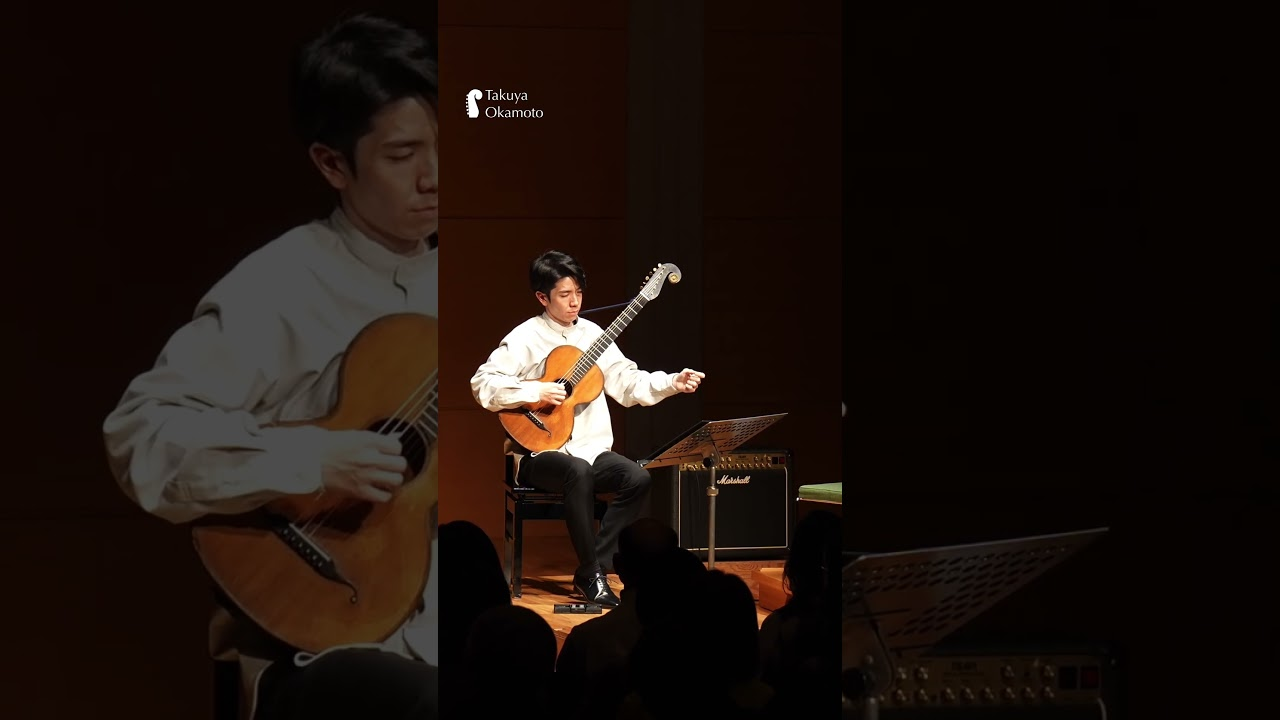
\includegraphics[width=0.48\linewidth]{pictures/youtube/2026/02/20260205_233209_youtube_001_gasmVmlGAeA.jpg}
}
\end{center}



ギターへの編曲はご本人によるものでしょうか？この楽譜（

\url{https://www.gendaiguitar.com/products/4539442046704}

）ではない様です。


（岡本拓也氏の他の演奏）

バッハ：BWV645

\url{https://www.facebook.com/100002225117991/posts/9969916699759068/}



バッハ：BWV998

\url{https://www.facebook.com/100002225117991/posts/9582585461825529/}



武満徹：波の盆

\url{https://www.facebook.com/100002225117991/posts/7979642405453184/}




===

この記事は、こちら↓の記事の続きです

\url{https://www.facebook.com/100002225117991/posts/24613905911600238/}




===

「ギターでマタイ受難曲」はここ↓

\url{https://m.facebook.com/story.php?story_fbid=26362889510035194&id=100002225117991}



\subsection*{2026年02月06日 03:16}
\addcontentsline{toc}{subsection}{2026年02月06日 03:16}

\paragraph{リンク}
\url{https://youtu.be/kqQtn5-UzxU}

\begin{center}
\href{https://youtu.be/kqQtn5-UzxU}{
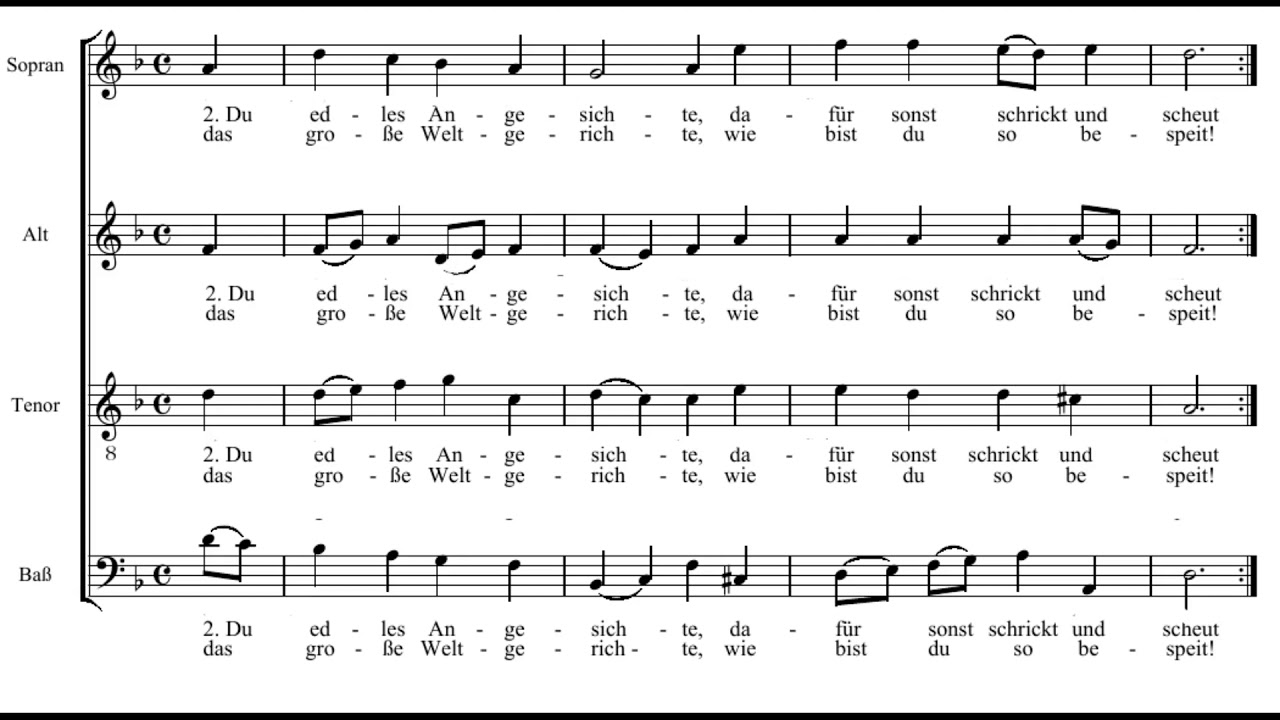
\includegraphics[width=0.48\linewidth]{pictures/youtube/2026/02/20260206_031605_youtube_001_kqQtn5-UzxU.jpg}
}
\end{center}

\subsection*{2026年02月06日 03:49}
\addcontentsline{toc}{subsection}{2026年02月06日 03:49}

\paragraph{リンク}
\url{https://youtu.be/uaSNwLv7V5Y}

\begin{center}
\href{https://youtu.be/uaSNwLv7V5Y}{
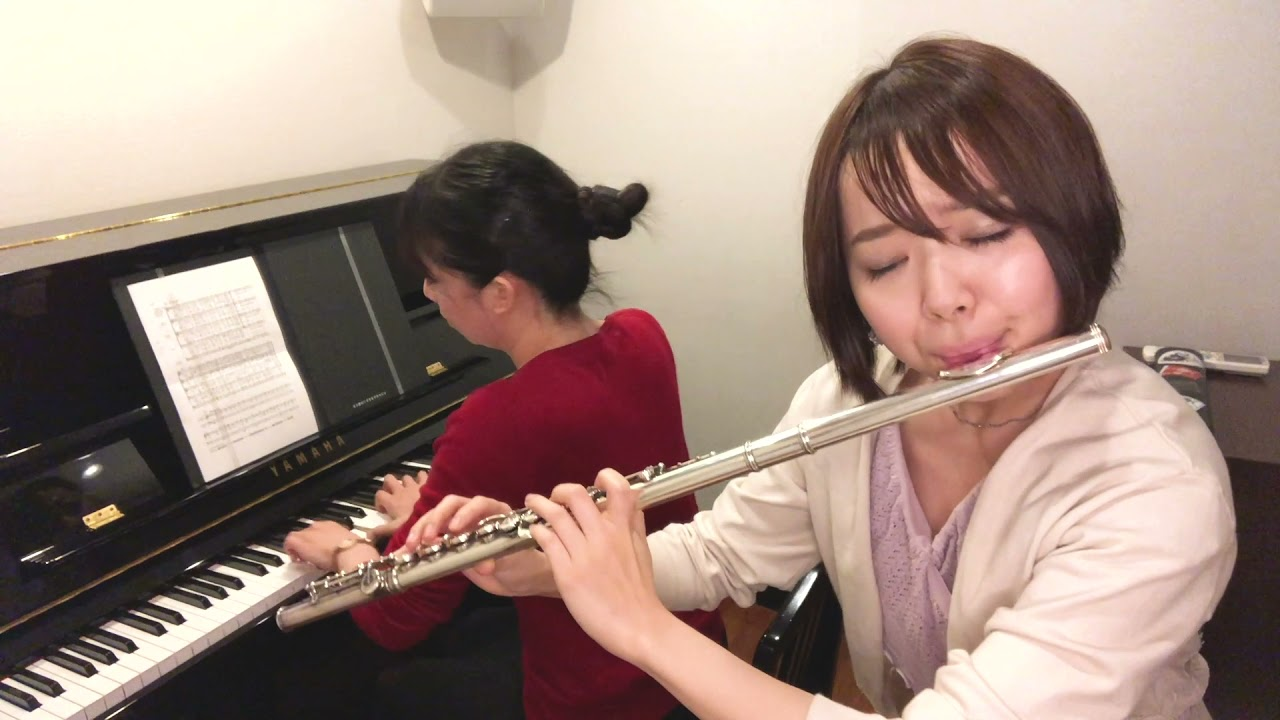
\includegraphics[width=0.48\linewidth]{pictures/youtube/2026/02/20260206_034952_youtube_001_uaSNwLv7V5Y.jpg}
}
\end{center}

\subsection*{2026年02月06日 04:11}
\addcontentsline{toc}{subsection}{2026年02月06日 04:11}

\paragraph{リンク}
\url{https://youtu.be/8mkjmPSnqYY}

\begin{center}
\href{https://youtu.be/8mkjmPSnqYY}{
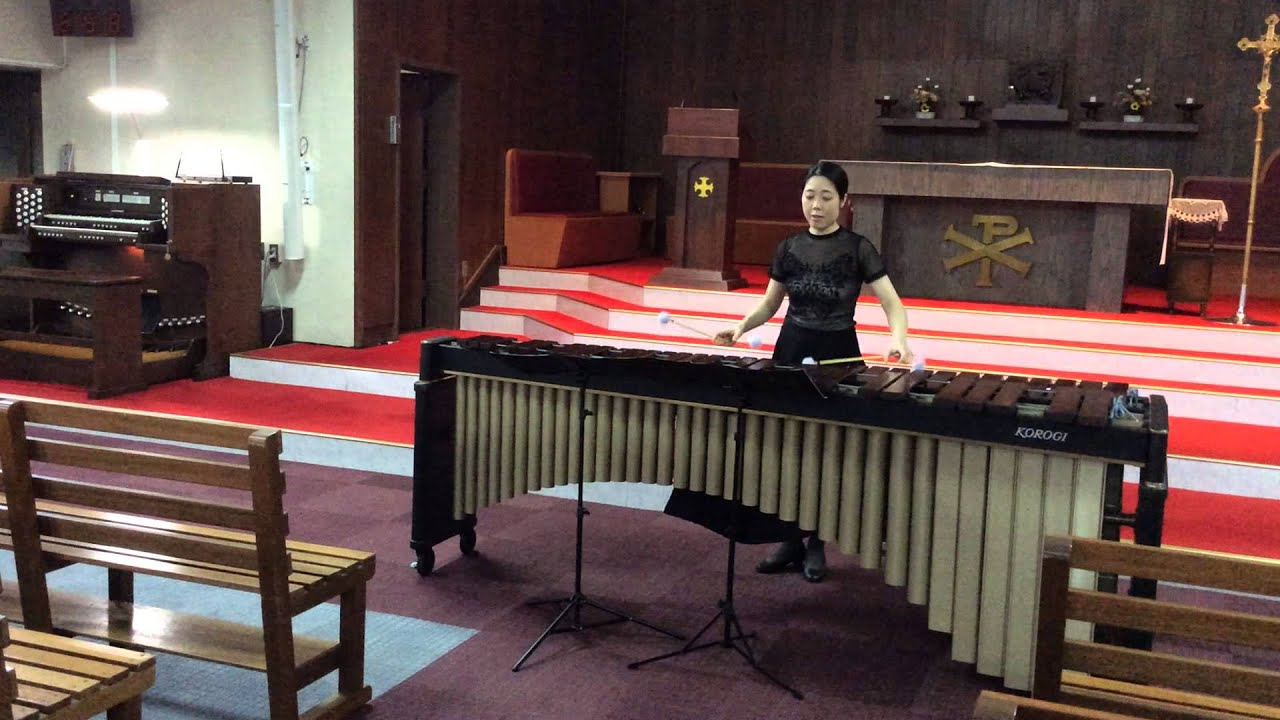
\includegraphics[width=0.48\linewidth]{pictures/youtube/2026/02/20260206_041156_youtube_001_8mkjmPSnqYY.jpg}
}
\end{center}

\subsection*{2026年02月06日 15:52}
\addcontentsline{toc}{subsection}{2026年02月06日 15:52}

\paragraph{リンク}
\url{https://youtu.be/Zry9dpM1_n4}

\begin{center}
\href{https://youtu.be/Zry9dpM1_n4}{
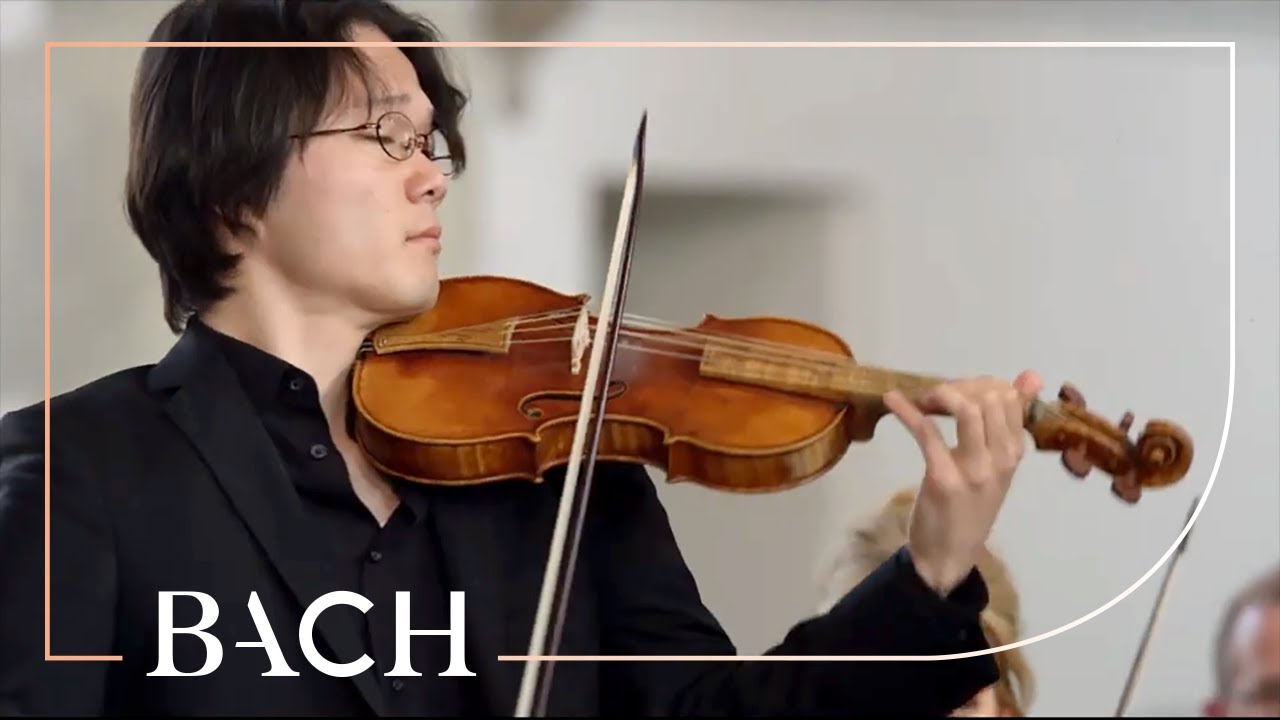
\includegraphics[width=0.48\linewidth]{pictures/youtube/2026/02/20260206_155234_youtube_001_Zry9dpM1_n4.jpg}
}
\end{center}

\subsection*{2026年02月07日 07:04}
\addcontentsline{toc}{subsection}{2026年02月07日 07:04}

マタイ受難曲（BWV244）よりErbarme dich


Erbarme dichのギター編を見つけた

\url{https://youtu.be/9cEHNXsVly8}

\begin{center}
\href{https://youtu.be/9cEHNXsVly8}{
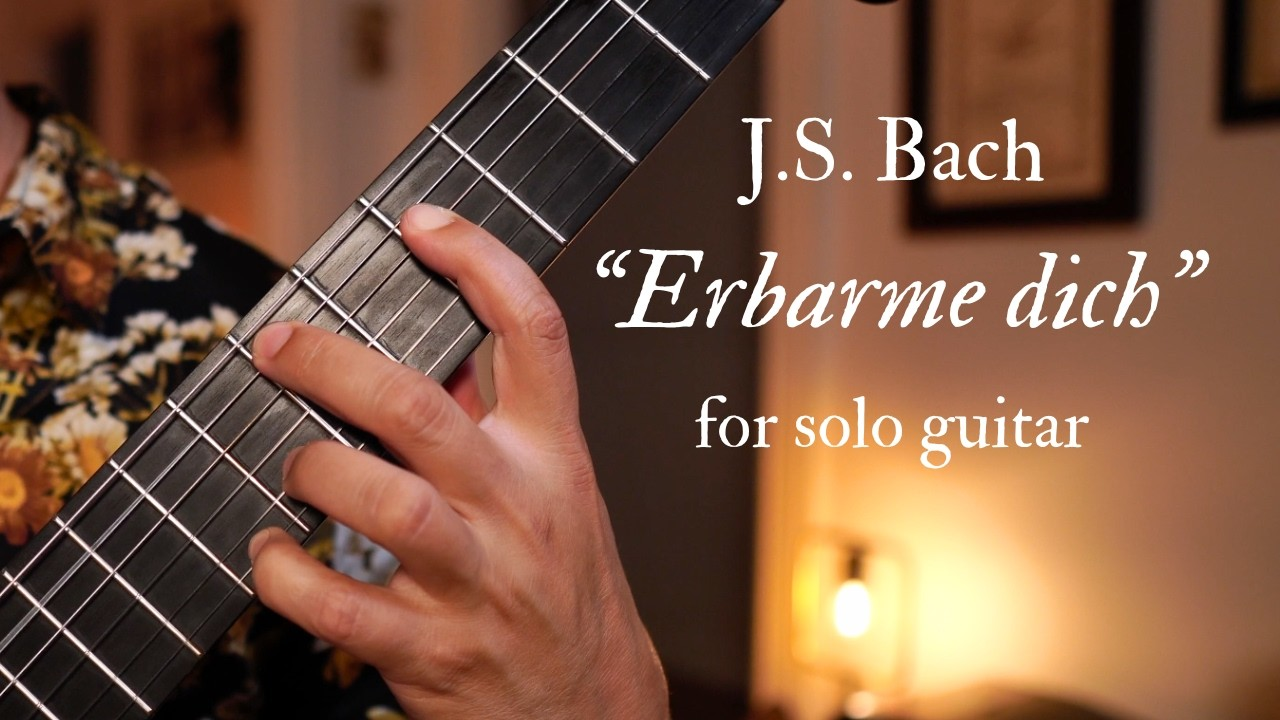
\includegraphics[width=0.48\linewidth]{pictures/youtube/2026/02/20260207_070416_youtube_001_9cEHNXsVly8.jpg}
}
\end{center}



PDF楽譜はここ↓から（ダウンロード\$12.00）

\url{https://tariqharb.com/product/bach-erbarme-dich-mein-gott-aria-from-st-matthew-passion-bwv-244-arr-harb/}




===

この記事は、以下↓の記事の続きです

\url{https://www.facebook.com/100002225117991/posts/25730484673275684/}




直接的にはこれ↓の続きかな？

\url{https://www.facebook.com/100002225117991/posts/9885193031564769/}




===

「ギターでマタイ受難曲」はここ↓

\url{https://m.facebook.com/story.php?story_fbid=26362889510035194&id=100002225117991}



\subsection*{2026年02月07日 08:46}
\addcontentsline{toc}{subsection}{2026年02月07日 08:46}

\paragraph{リンク}
\url{https://youtu.be/fqG-BOk9QHo}

\begin{center}
\href{https://youtu.be/fqG-BOk9QHo}{
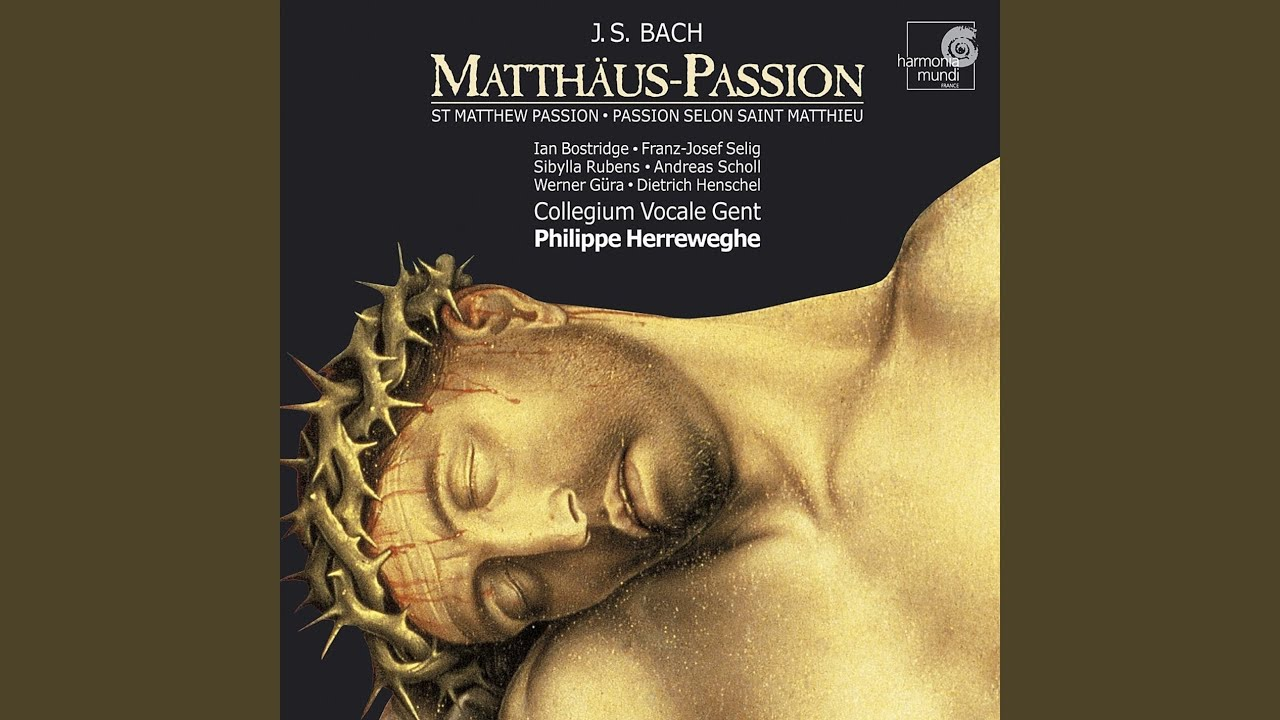
\includegraphics[width=0.48\linewidth]{pictures/youtube/2026/02/20260207_084636_youtube_001_fqG-BOk9QHo.jpg}
}
\end{center}

\subsection*{2026年02月08日 15:18}
\addcontentsline{toc}{subsection}{2026年02月08日 15:18}

\paragraph{リンク}
\url{https://youtu.be/OvGs6w6_WJw}

\begin{center}
\href{https://youtu.be/OvGs6w6_WJw}{
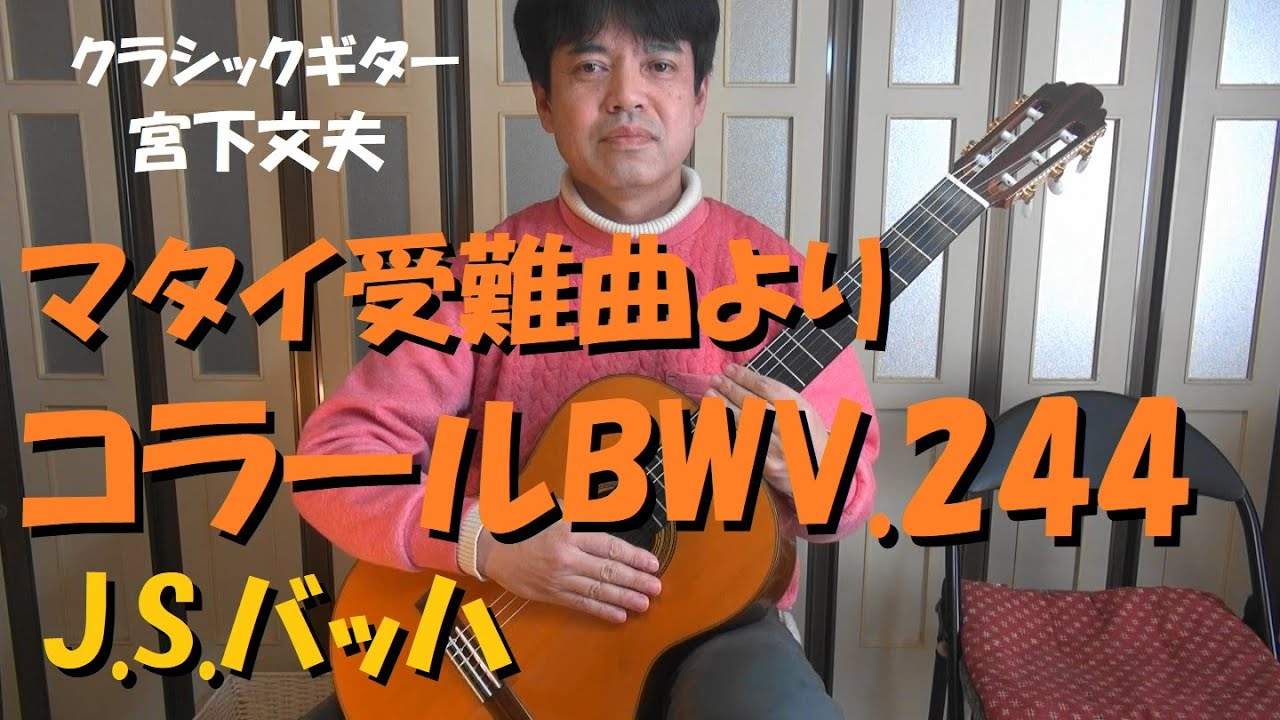
\includegraphics[width=0.48\linewidth]{pictures/youtube/2026/02/20260208_151831_youtube_001_OvGs6w6_WJw.jpg}
}
\end{center}

\subsection*{2026年02月09日 07:08}
\addcontentsline{toc}{subsection}{2026年02月09日 07:08}

この方、ロボットみたいな厳しい指の動きで、素敵な音を奏でていらっしゃいます。ここのリンクに集めたのは、カタロニア民謡からメジャーな３曲と、バッハのシャコンヌです。この方の演奏どれも素晴らしいですね。楽しめています。


聖母の御子

\url{https://youtu.be/S9zTg8Ykdp0}

\begin{center}
\href{https://youtu.be/S9zTg8Ykdp0}{
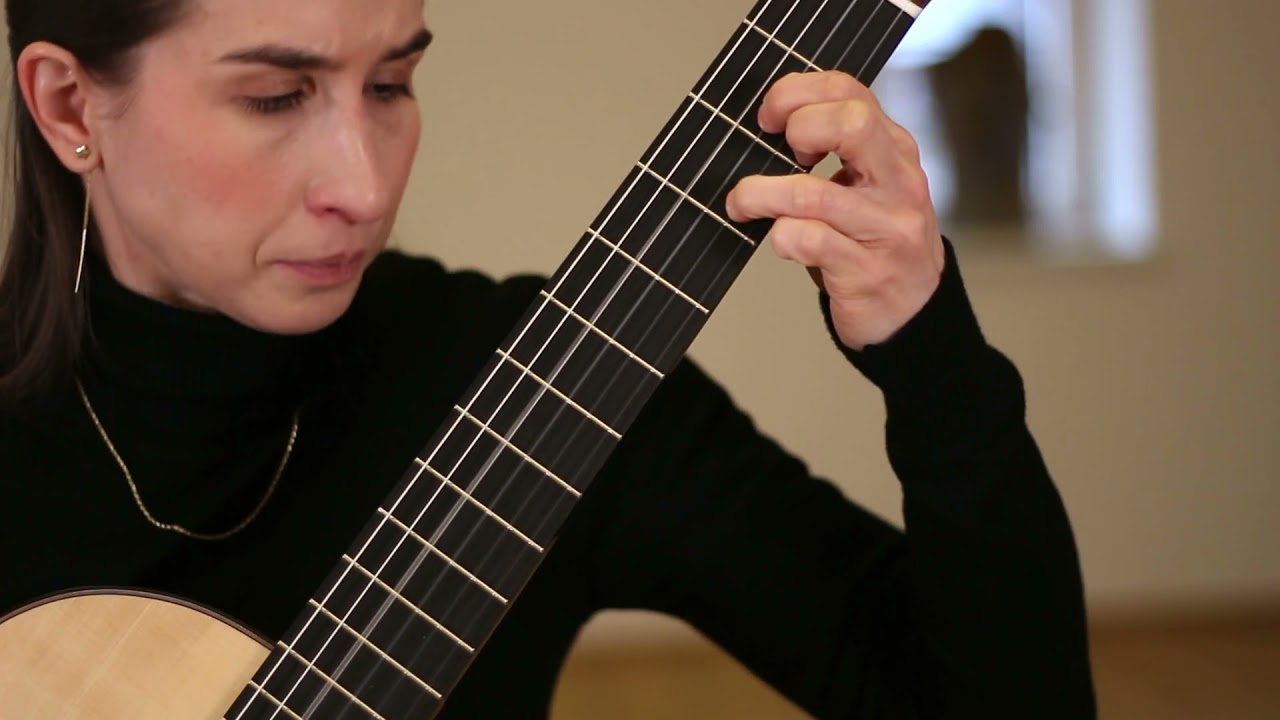
\includegraphics[width=0.48\linewidth]{pictures/youtube/2026/02/20260209_070804_youtube_001_S9zTg8Ykdp0.jpg}
}
\end{center}



盗賊の歌

\url{https://youtu.be/QVVxeHj-ENE}

\begin{center}
\href{https://youtu.be/QVVxeHj-ENE}{
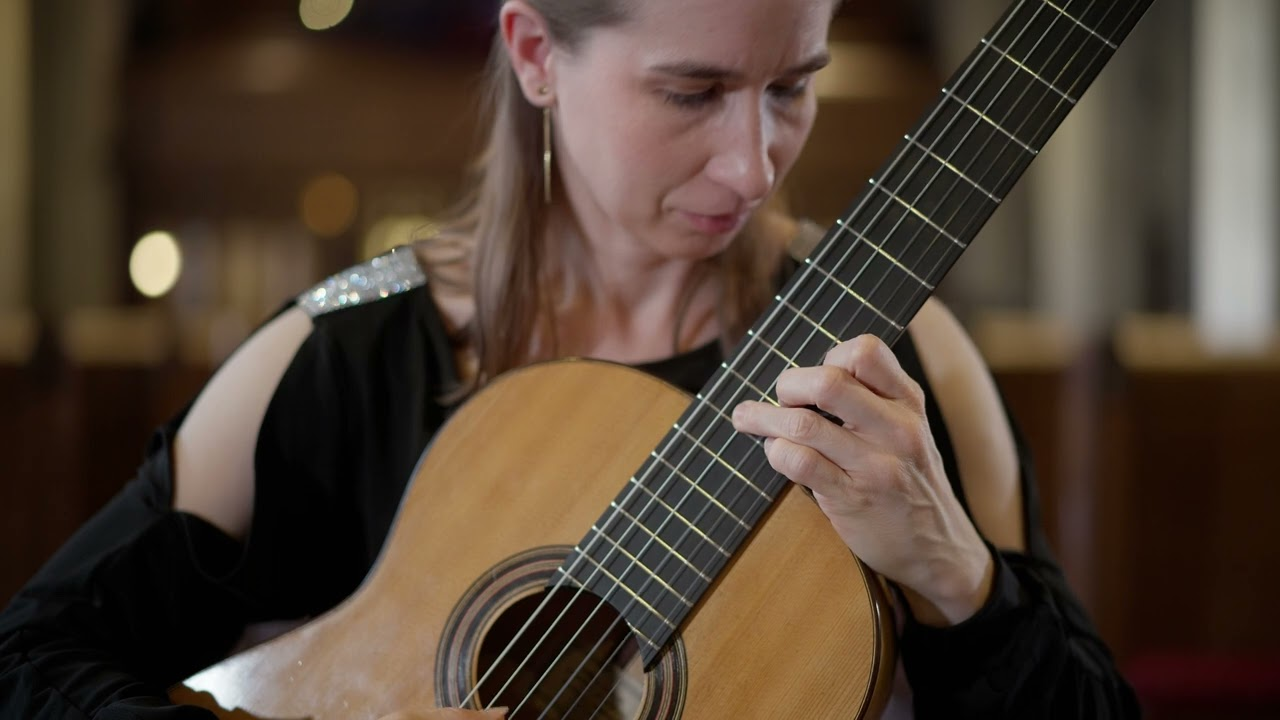
\includegraphics[width=0.48\linewidth]{pictures/youtube/2026/02/20260209_070804_youtube_002_QVVxeHj-ENE.jpg}
}
\end{center}



アメリアの遺言

\url{https://www.facebook.com/100002225117991/posts/8871339149616834/}



シャコンヌ

\url{https://www.facebook.com/100002225117991/posts/8370443646373056/}




ただ、聖母の御子の演奏についてちょっとだけ気になるのは、、、やっぱり4小節目の真ん中の和音だけは気になります（繰り返しでも同じ和音を鳴らしていらっしゃる）


聖母の御子のリョベート編による演奏はこれ↓

\url{https://www.facebook.com/100002225117991/posts/8813271782090238/}



リョベート編でない楽譜の存在については、ここ↓でも気にしていた

\url{https://m.facebook.com/story.php?story_fbid=8994872797263468&id=100002225117991}



\subsection*{2026年02月09日 13:18}
\addcontentsline{toc}{subsection}{2026年02月09日 13:18}

コーヒーは、


(１)サイフォンで淹れると「苦くなる」。これはロートに湯が滞在する（煮込み？の）時間によって調整できる事なんだろうけど。（１分間滞在させると充分苦くなる気がする）

(２)ドリップで淹れると苦くない。どちらかと言えば「サッパリした仕上がり」になる。これはコーヒーの粉を湯がサッと通り過ぎるためだろうか。色々なrecipeが提案されてはいるが、面倒なことはしたくない。少し蒸らしたら、後は「ゆっくり」最終容量までお湯を注ぐだけだ。（←これがサッパリする仕上がりの原因かもしれない）


１回に２杯位は飲みたくなるので、特にドリップの際には（添付の表↓を頼りにして）、豆21g×率16.5=注ぐ湯の量346.5cc（→仕上がり約300cc）としてみている。（添付の表の出典は 

\url{https://youtu.be/Tl97tMmyLX4}

\begin{center}
\href{https://youtu.be/Tl97tMmyLX4}{
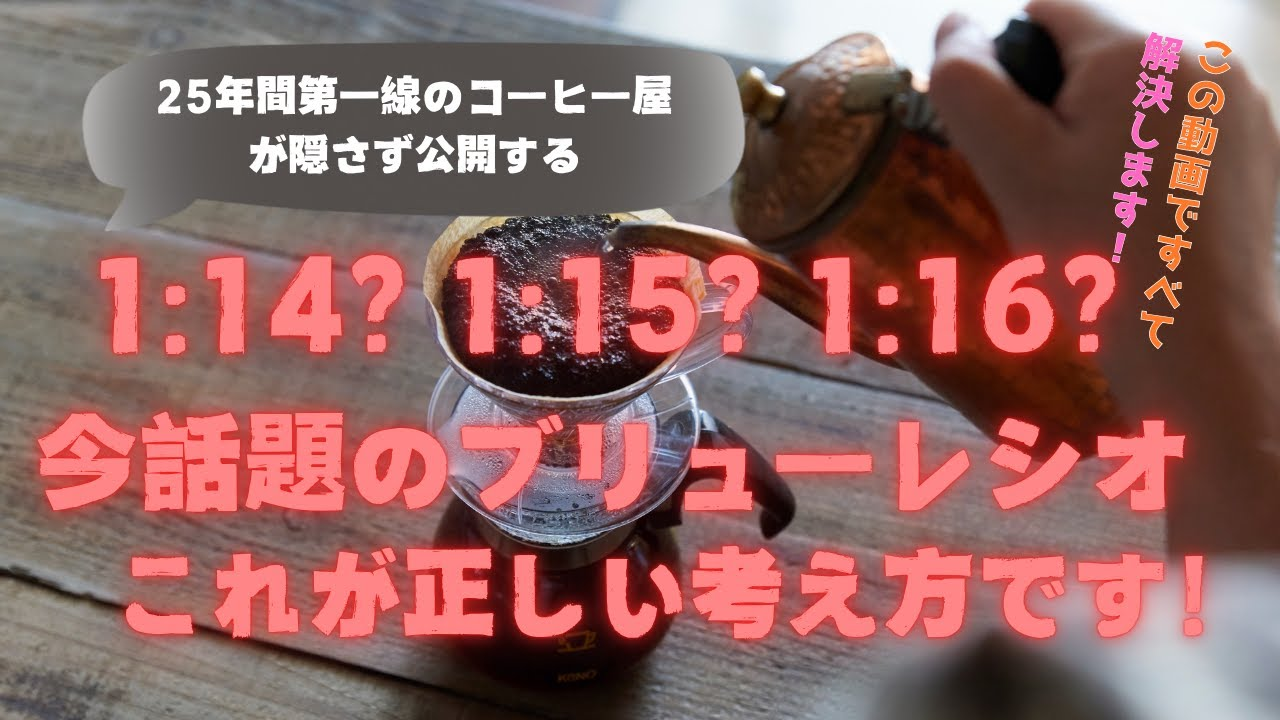
\includegraphics[width=0.48\linewidth]{pictures/youtube/2026/02/20260209_131816_youtube_001_Tl97tMmyLX4.jpg}
}
\end{center}

 ）


===

この記事は、以下↓の記事の続きです

\url{https://m.facebook.com/story.php?story_fbid=25623563003967852&id=100002225117991}



\paragraph{写真}
\begin{center}
\begin{minipage}{0.48\linewidth}
\centering
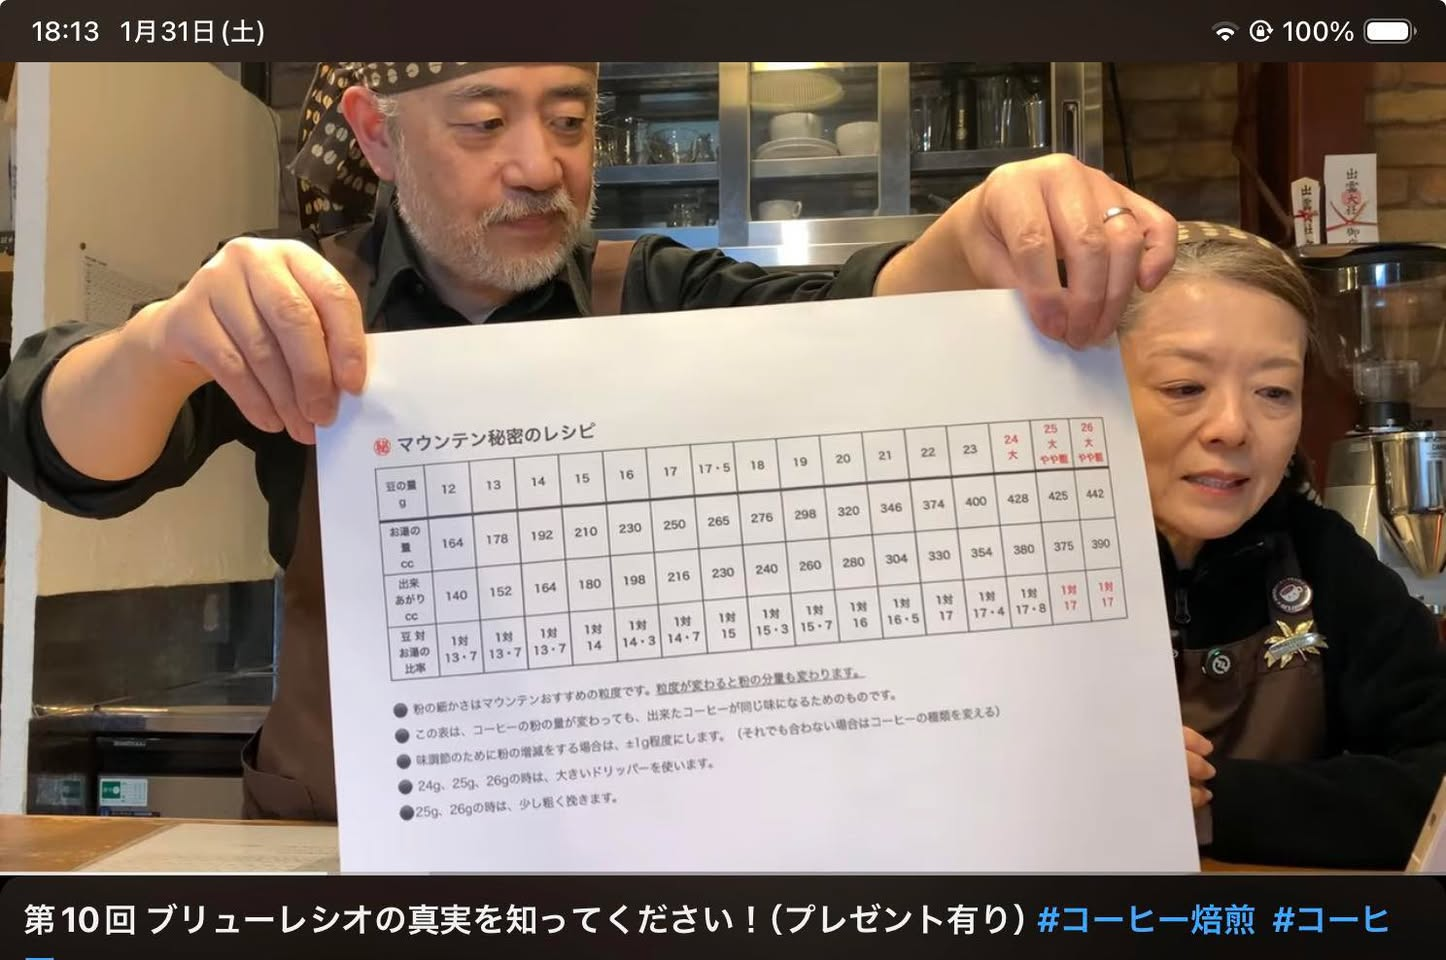
\includegraphics[width=\linewidth]{pictures/2026/02/20260209_131816_001.jpg}
\end{minipage}
\end{center}

\subsection*{2026年02月09日 15:11}
\addcontentsline{toc}{subsection}{2026年02月09日 15:11}

練習中のBWV998のFugueについて、やっぱり運指を見直す事にした


Youtubeの映像をあれこれ見るにつけ、どの方も（基本は）セゴビア編の運指なんだという事を確信してきました


問題の多くは、難所の大部分が存在している所、即ち第45小節から第65小節に至るダイナミックな「音の上下降が繰り返される」所にあるのですが。


Segovia編の様に、左のフレット、第１ポジション寄りを優先させて使う事による生き生きとした音の動きは、Scheit編の様に、右のフレット、高いポジションで「コソコソ鳴らして」いたり、第４〜６弦辺りで「モゾモゾ鳴らして」いたりするのと比べたら、「音符上は同じ音を鳴らしているのに」外に向けて表現できているものは、全く違ったものになっているじゃないかと思う様になった。


という事で、今はSegovia編の運指をチマチマ追ってみている所です。


===

話は変わりますが、以下を英訳するとどうなりますか？

(１)あれこれ

(２)コソコソ

(３)モゾモゾ

(４)チマチマ

ChatGPTに聞いてみようかな


===

この記事は、以下↓の記事の続きです

\url{https://www.facebook.com/100002225117991/posts/25714855218171963/}



\subsection*{2026年02月09日 23:05}
\addcontentsline{toc}{subsection}{2026年02月09日 23:05}

\paragraph{リンク}
\url{https://youtu.be/S9zTg8Ykdp0}

\begin{center}
\href{https://youtu.be/S9zTg8Ykdp0}{
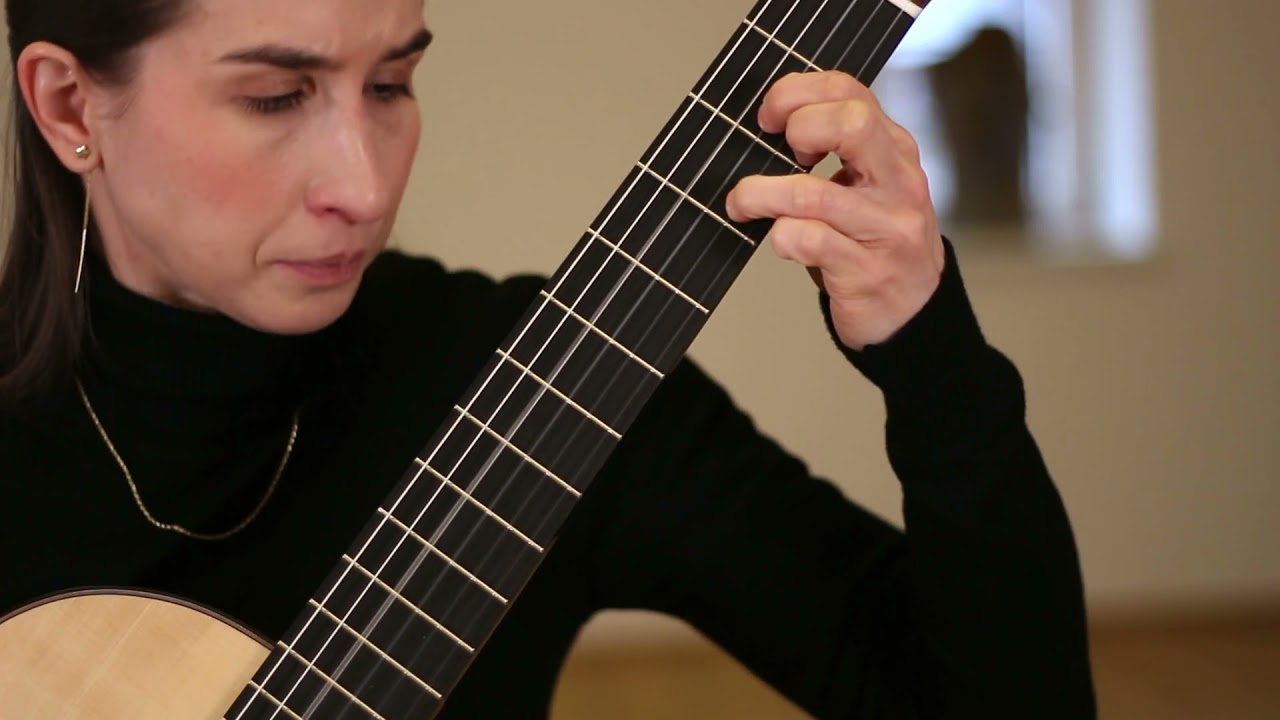
\includegraphics[width=0.48\linewidth]{pictures/youtube/2026/02/20260209_230503_youtube_001_S9zTg8Ykdp0.jpg}
}
\end{center}

\subsection*{2026年02月10日 16:02}
\addcontentsline{toc}{subsection}{2026年02月10日 16:02}

\paragraph{リンク}
\url{http://deepl.com/}

\subsection*{2026年02月10日 23:34}
\addcontentsline{toc}{subsection}{2026年02月10日 23:34}

何か素敵な言葉だなぁ「Articulation Silences」←どう鳴らしたらいい？

（「静寂の表情」か？）言葉では表せないニュアンス（トラヴェルソなら表現できる？）


以下、連想ゲームになってしまいました（お許し下さいませ）


(１)「Sound of Silence」というのもありました

(２)M.Ravelのダフニスとクロエより夜明け(←「シーン」という「音」の表情を「鳴らす」)

\url{https://m.facebook.com/story.php?story_fbid=23876936348630535&id=100002225117991}



(３)ジョン・ケージの４分33秒は？（←nothing but a joke！）静寂の表情を表現できる？


===

\url{https://m.facebook.com/groups/170274089697446/permalink/25957005460597622/}



\subsection*{2026年02月11日 09:49}
\addcontentsline{toc}{subsection}{2026年02月11日 09:49}

これは公開しない


\url{https://www.facebook.com/groups/1052176425293516/permalink/2341106536400492/}




\url{https://www.facebook.com/100003050293182/posts/25594973466854312/}




\url{https://m.facebook.com/groups/1052176425293516/permalink/2344122636098882/}



\paragraph{写真}
\begin{center}
\begin{minipage}{0.48\linewidth}
\centering
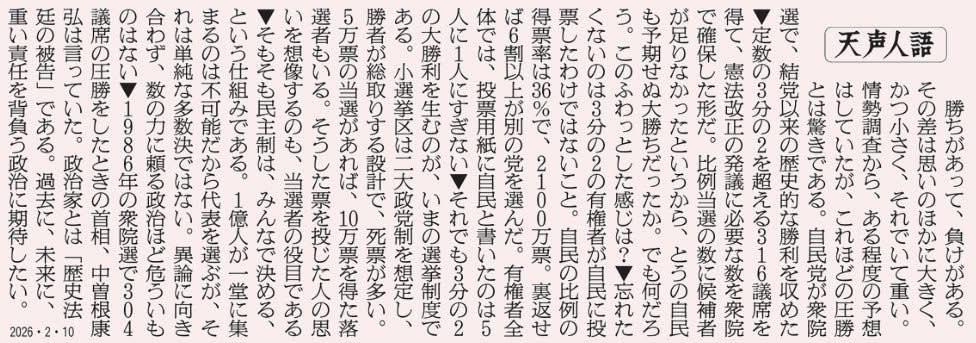
\includegraphics[width=\linewidth]{pictures/2026/02/20260211_094949_001.jpg}
\end{minipage}
\hfill
\begin{minipage}{0.48\linewidth}
\centering
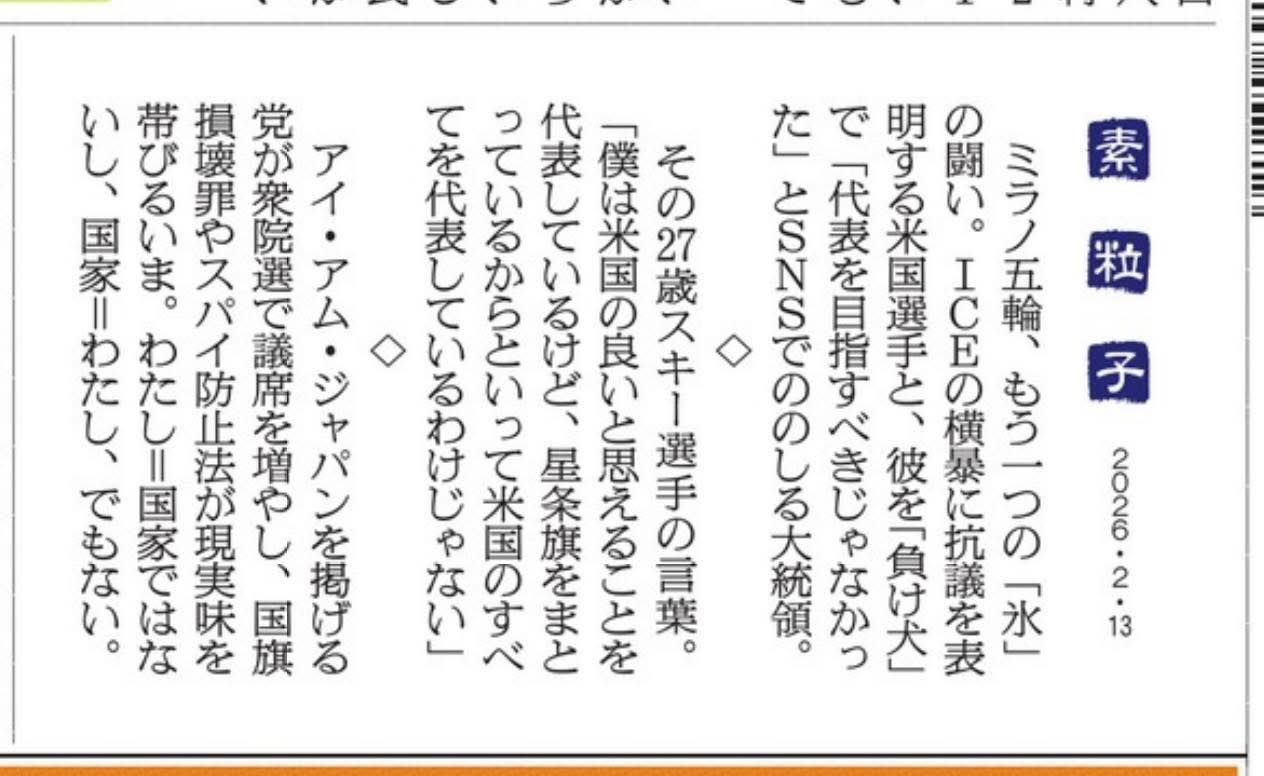
\includegraphics[width=\linewidth]{pictures/2026/02/20260211_094949_002.jpg}
\end{minipage}
\end{center}

\begin{center}
\begin{minipage}{0.48\linewidth}
\centering
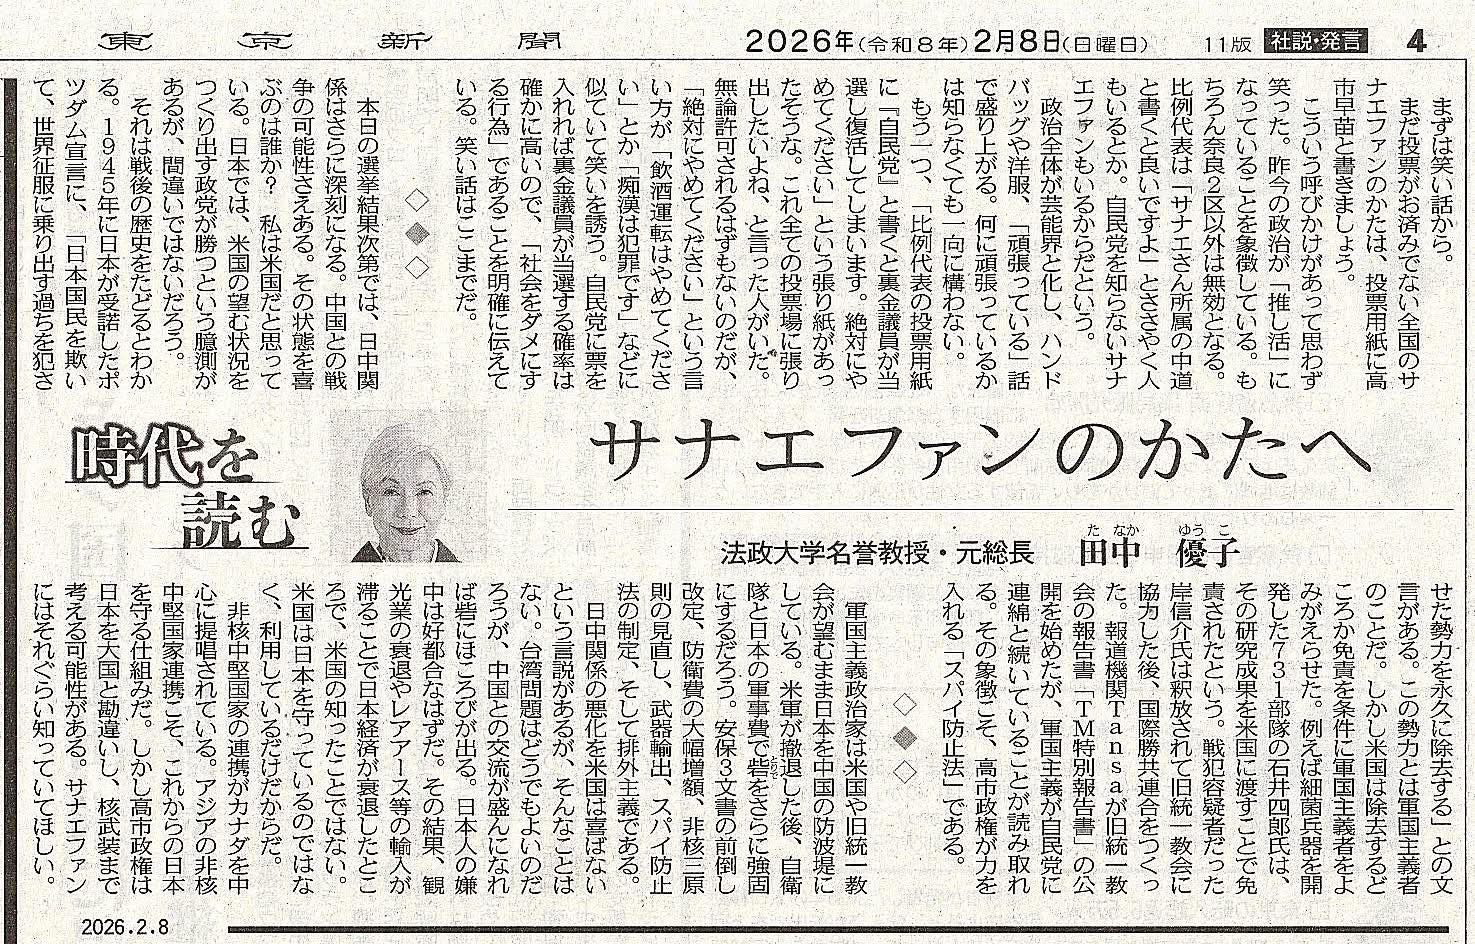
\includegraphics[width=\linewidth]{pictures/2026/02/20260211_094949_003.jpg}
\end{minipage}
\hfill
\begin{minipage}{0.48\linewidth}
\centering
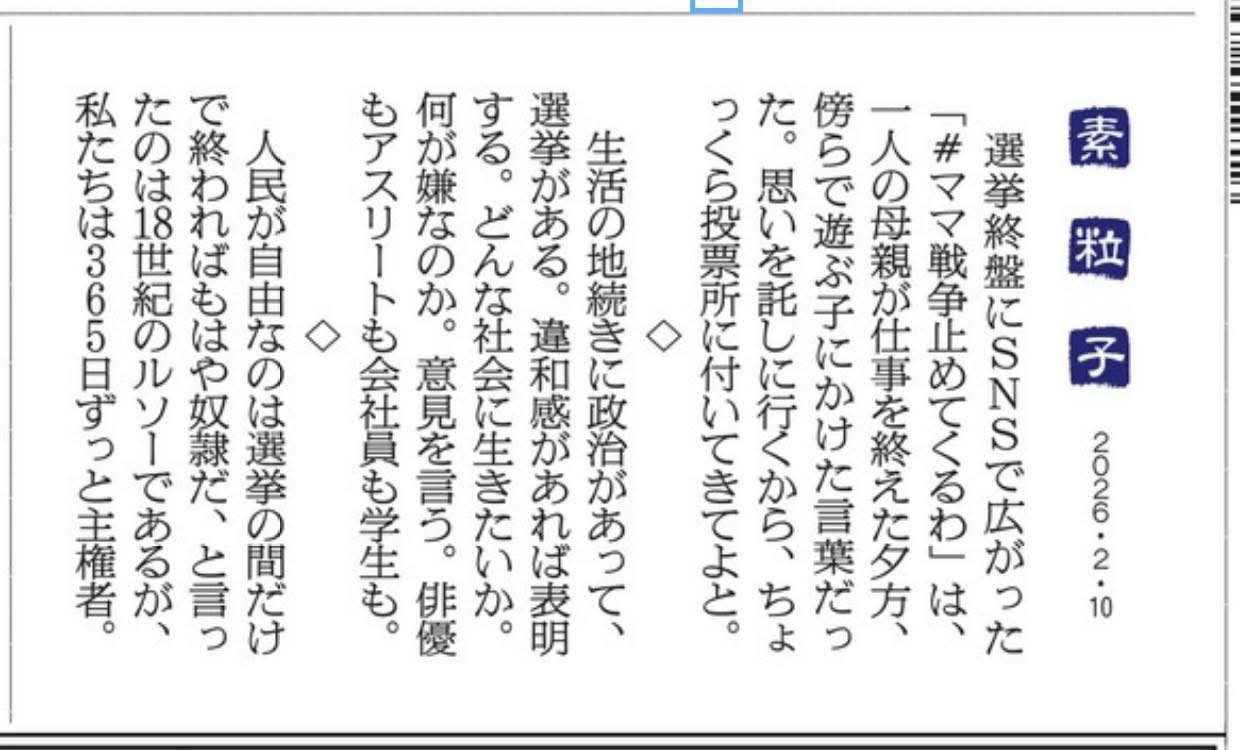
\includegraphics[width=\linewidth]{pictures/2026/02/20260211_094949_004.jpg}
\end{minipage}
\end{center}

\subsection*{2026年02月13日 03:35}
\addcontentsline{toc}{subsection}{2026年02月13日 03:35}

\paragraph{リンク}
\url{https://youtu.be/3W-SdpmUb5g}

\begin{center}
\href{https://youtu.be/3W-SdpmUb5g}{
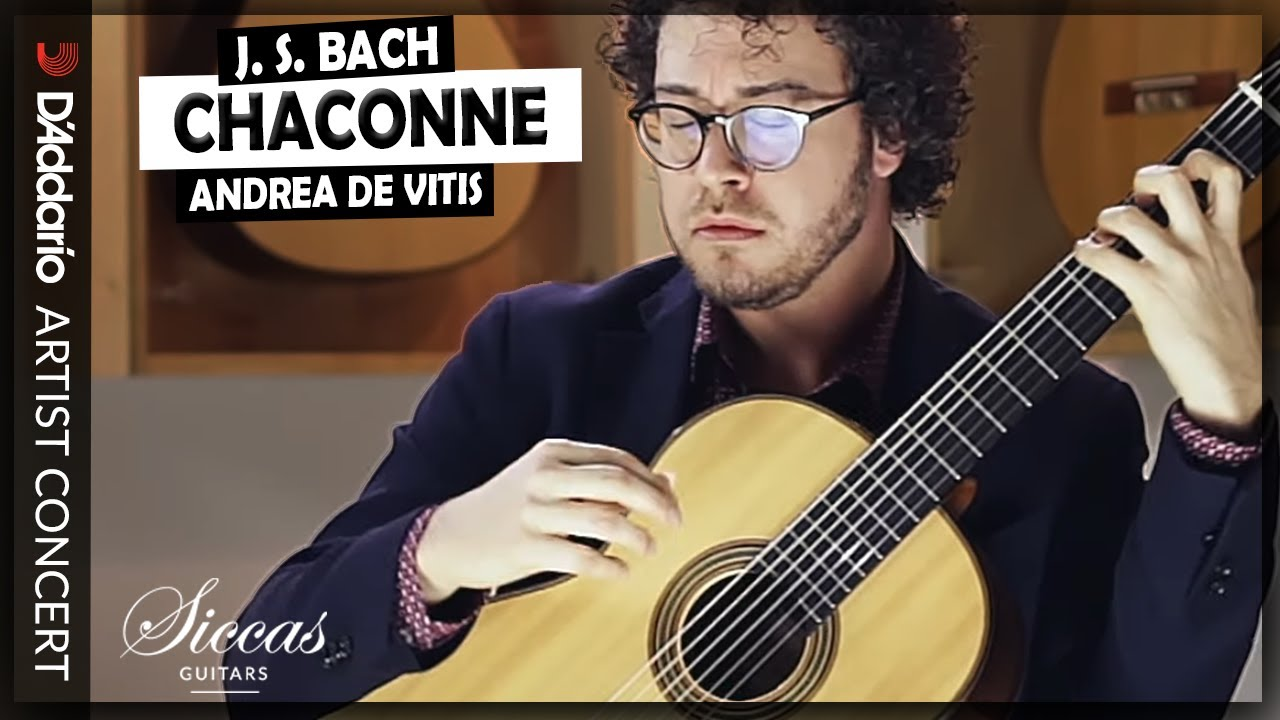
\includegraphics[width=0.48\linewidth]{pictures/youtube/2026/02/20260213_033503_youtube_001_3W-SdpmUb5g.jpg}
}
\end{center}

\subsection*{2026年02月14日 11:19}
\addcontentsline{toc}{subsection}{2026年02月14日 11:19}

\paragraph{リンク}
\url{https://youtu.be/4-ra2Rq5NGQ}

\begin{center}
\href{https://youtu.be/4-ra2Rq5NGQ}{
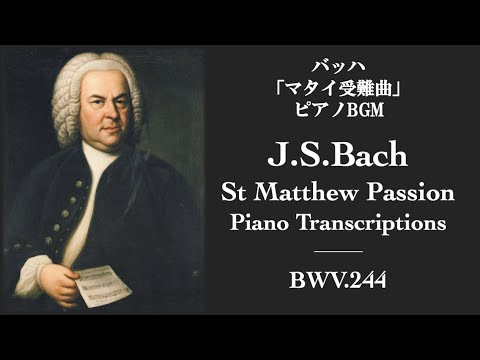
\includegraphics[width=0.48\linewidth]{pictures/youtube/2026/02/20260214_111949_youtube_001_4-ra2Rq5NGQ.jpg}
}
\end{center}

\subsection*{2026年02月14日 17:44}
\addcontentsline{toc}{subsection}{2026年02月14日 17:44}

なるほど、それはあるかもしれない


\url{https://www.facebook.com/photo.php?fbid=10163350410877672&set=a.10150089862567672&type=3}



\subsection*{2026年02月14日 17:56}
\addcontentsline{toc}{subsection}{2026年02月14日 17:56}

C.A.Debussy （前奏曲集第１巻より）亜麻色の髪の乙女


(１)ジュリアン・ブリーム編

\url{https://youtu.be/bQhdlyzcFYI}

\begin{center}
\href{https://youtu.be/bQhdlyzcFYI}{
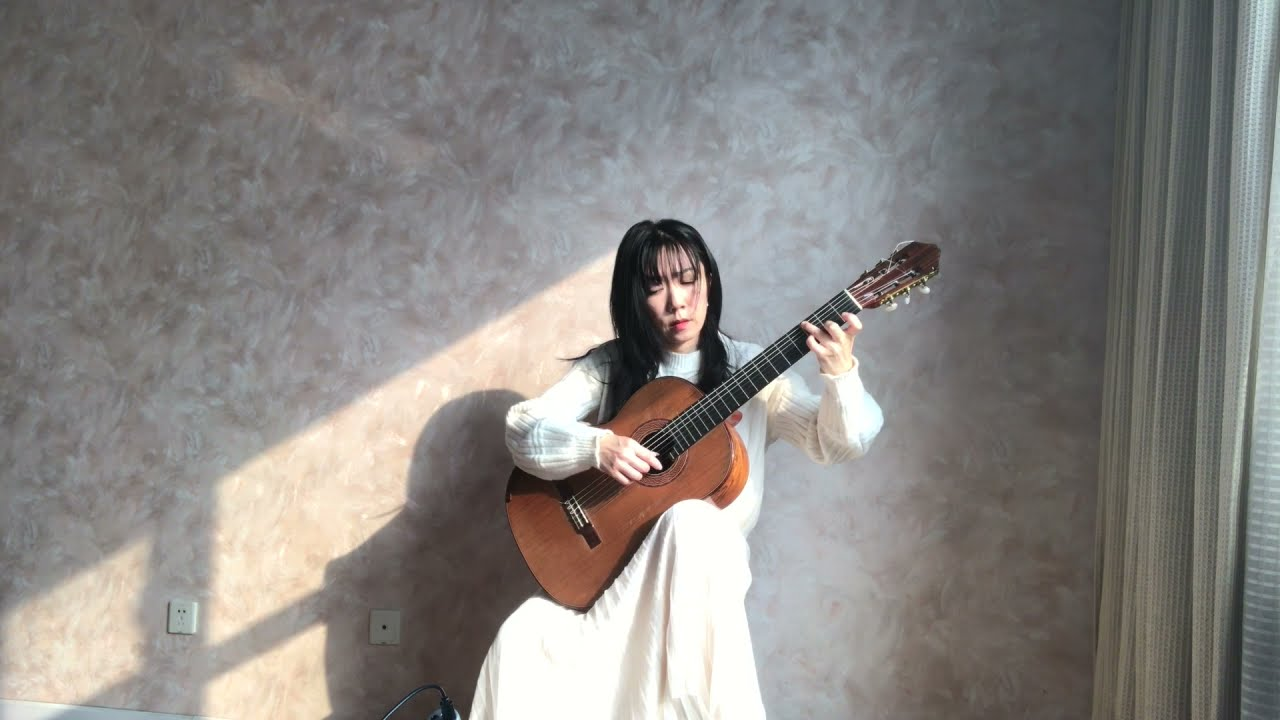
\includegraphics[width=0.48\linewidth]{pictures/youtube/2026/02/20260214_175635_youtube_001_bQhdlyzcFYI.jpg}
}
\end{center}



\url{https://youtu.be/ZDtH98ClV3s}

\begin{center}
\href{https://youtu.be/ZDtH98ClV3s}{
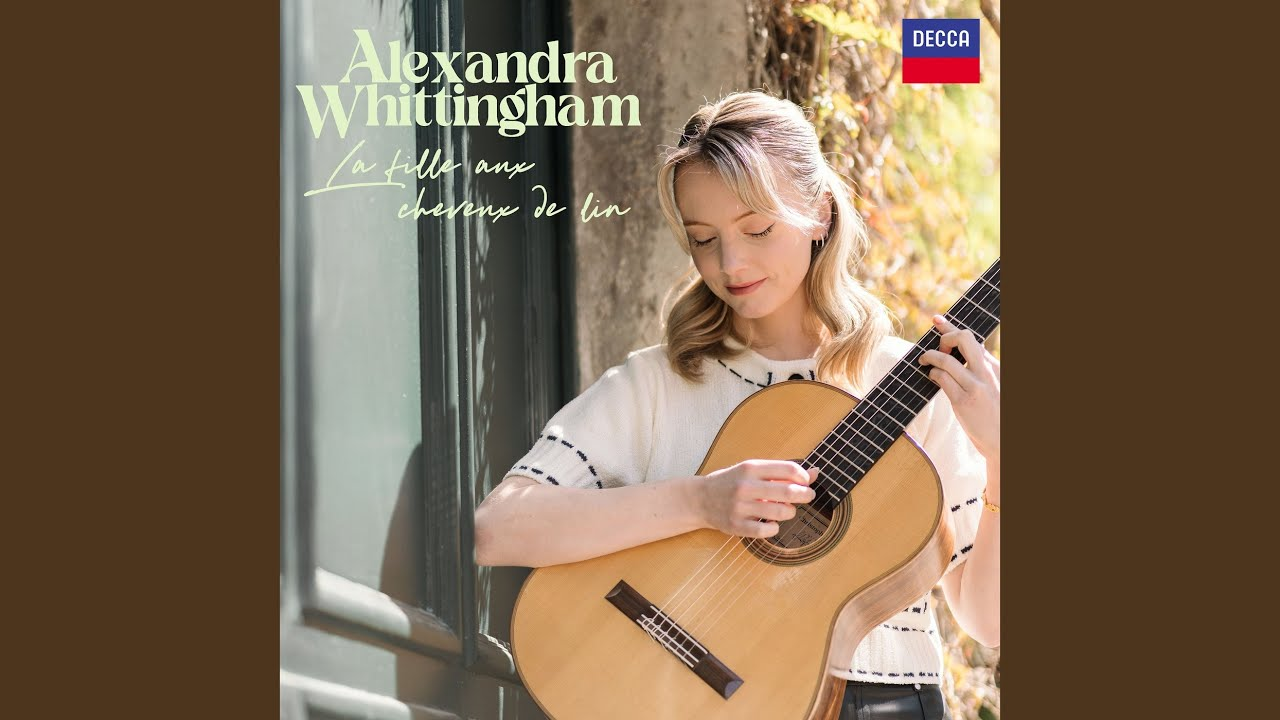
\includegraphics[width=0.48\linewidth]{pictures/youtube/2026/02/20260214_175635_youtube_002_ZDtH98ClV3s.jpg}
}
\end{center}




ブリーム編の楽譜はこれ（¥6,050 高い！）

\url{https://www.gendaiguitar.com/products/9780571538799}



この曲集について、こんな事↓が書いてある

「イギリスの老舗フェイバーミュージックによるクラシックギター名曲集。全48曲の中に、現在日本では入手困難なブリーム編の作品が多数収載されていて貴重」


目次からブリーム編を選択的に（チラッと）見た所によると、BachのBWV996（リュート組曲１番）や、Debussyでは前奏曲集から冒頭の曲の他にミンストレルも編曲されている様です。その他グリーグやモーツァルト等の編曲も載せられている。この楽譜集貴重なものなのかもしれませんが、高いのはしょうがない事なのか。（載っている曲の総数で割れば、１曲あたりの値段は他の曲集とそれほど変わらないのかもしれません）


(２)デイヴィッド・ラッセル編

\url{https://youtu.be/I9qxXDKS9ZA}

\begin{center}
\href{https://youtu.be/I9qxXDKS9ZA}{
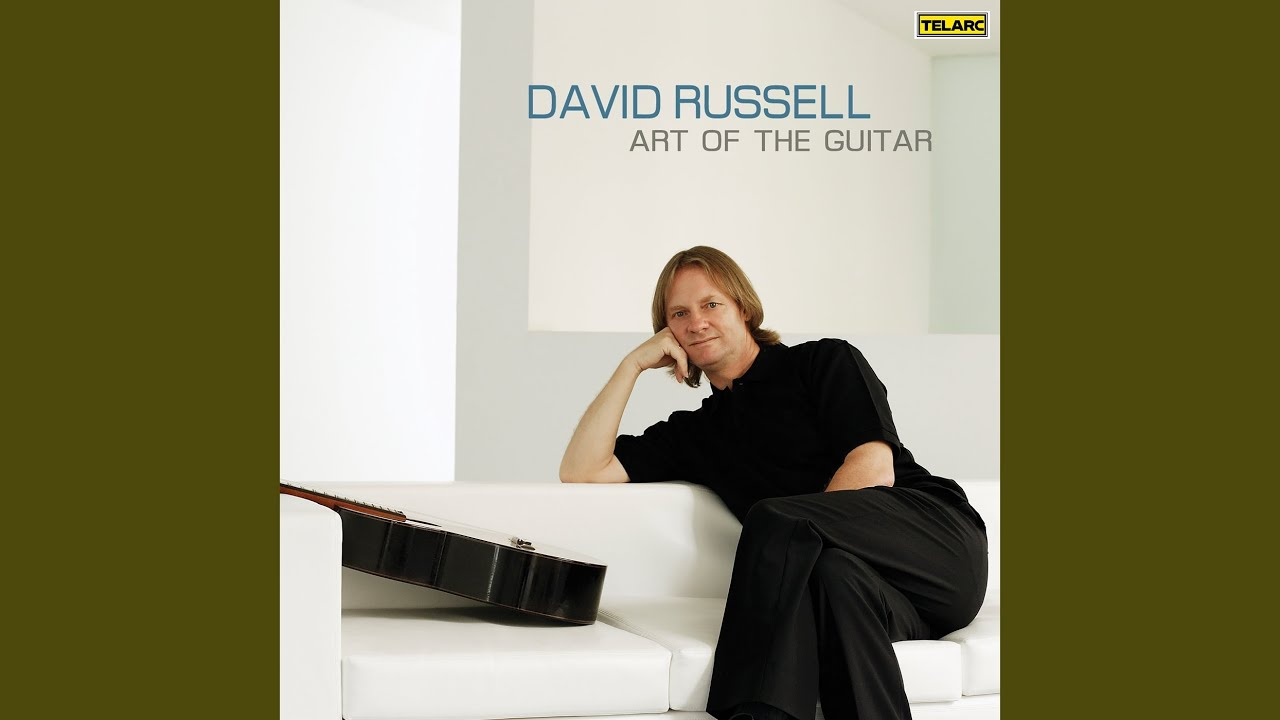
\includegraphics[width=0.48\linewidth]{pictures/youtube/2026/02/20260214_175635_youtube_003_I9qxXDKS9ZA.jpg}
}
\end{center}




ラッセル氏はBachやHandel等のバロックだけでなく、それ以外にDebussyの様な近代の曲でも編曲を手掛けていらしたのですね。（この曲のラッセル編による楽譜は見つけられなかった）


(３)ホセ・ルイス・ゴンザレス編

\url{https://youtu.be/ADkIe_eS_qM}

\begin{center}
\href{https://youtu.be/ADkIe_eS_qM}{
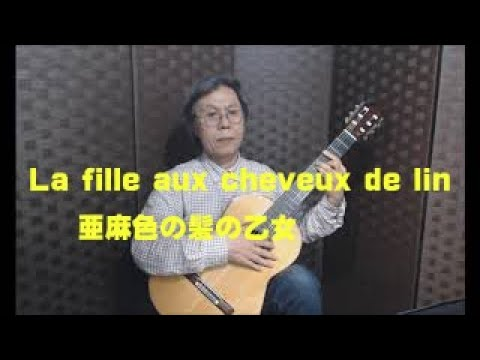
\includegraphics[width=0.48\linewidth]{pictures/youtube/2026/02/20260214_175635_youtube_004_ADkIe_eS_qM.jpg}
}
\end{center}




私の手元にある楽譜、GG（現代ギター）社の「てんこもりVol２」に載っているのは、ホセ・ルイス・ゴンザレス編。そう言えば、エストレリータもこの方の手による編曲（ 

\url{https://www.facebook.com/share/1DLv29VbaX/?mibextid=wwXIfr}

 ）でした。


===

この記事は、以下↓の記事の続きです

\url{https://www.facebook.com/100002225117991/posts/9970488753035196/}



或いは、

\url{https://m.facebook.com/story.php?story_fbid=24972048832452609&id=100002225117991}



\subsection*{2026年02月15日 02:21}
\addcontentsline{toc}{subsection}{2026年02月15日 02:21}

この方、トレモロがとってもお上手な様な気がする

\url{https://youtu.be/SbCDjfIVow0}

\begin{center}
\href{https://youtu.be/SbCDjfIVow0}{
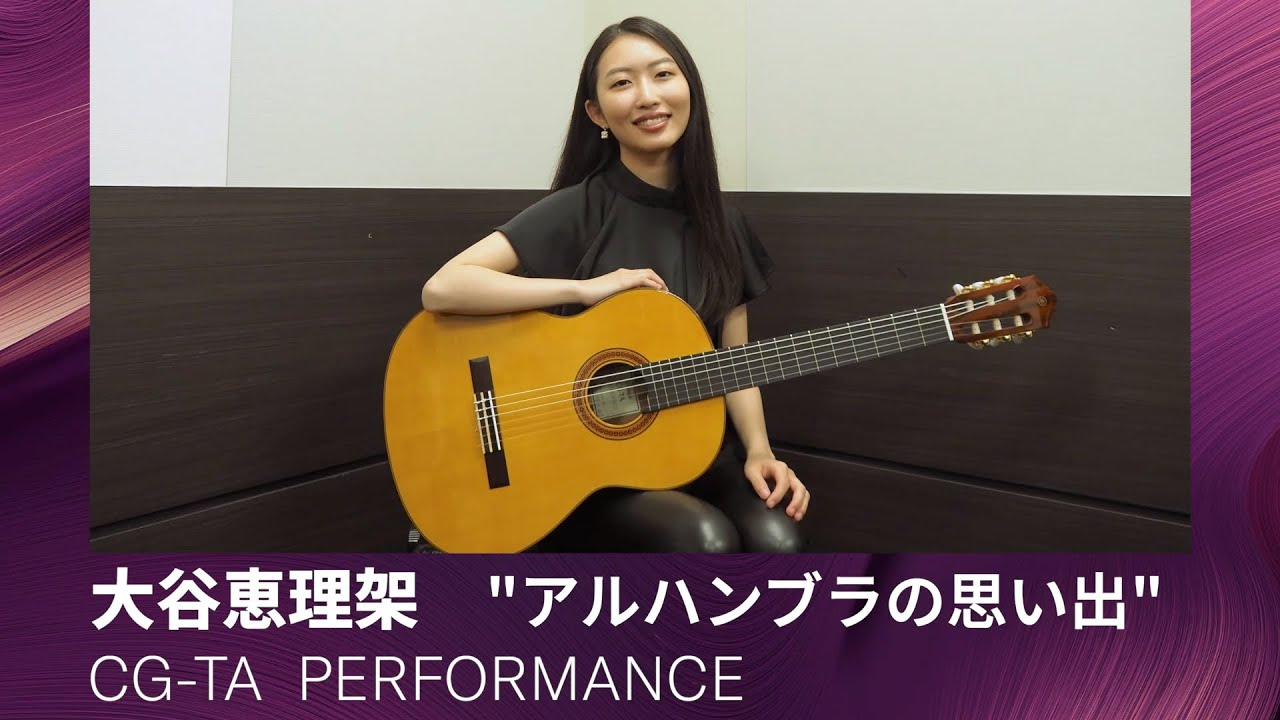
\includegraphics[width=0.48\linewidth]{pictures/youtube/2026/02/20260215_022157_youtube_001_SbCDjfIVow0.jpg}
}
\end{center}



\url{https://youtu.be/qhMkWOjO0Qs}

\begin{center}
\href{https://youtu.be/qhMkWOjO0Qs}{
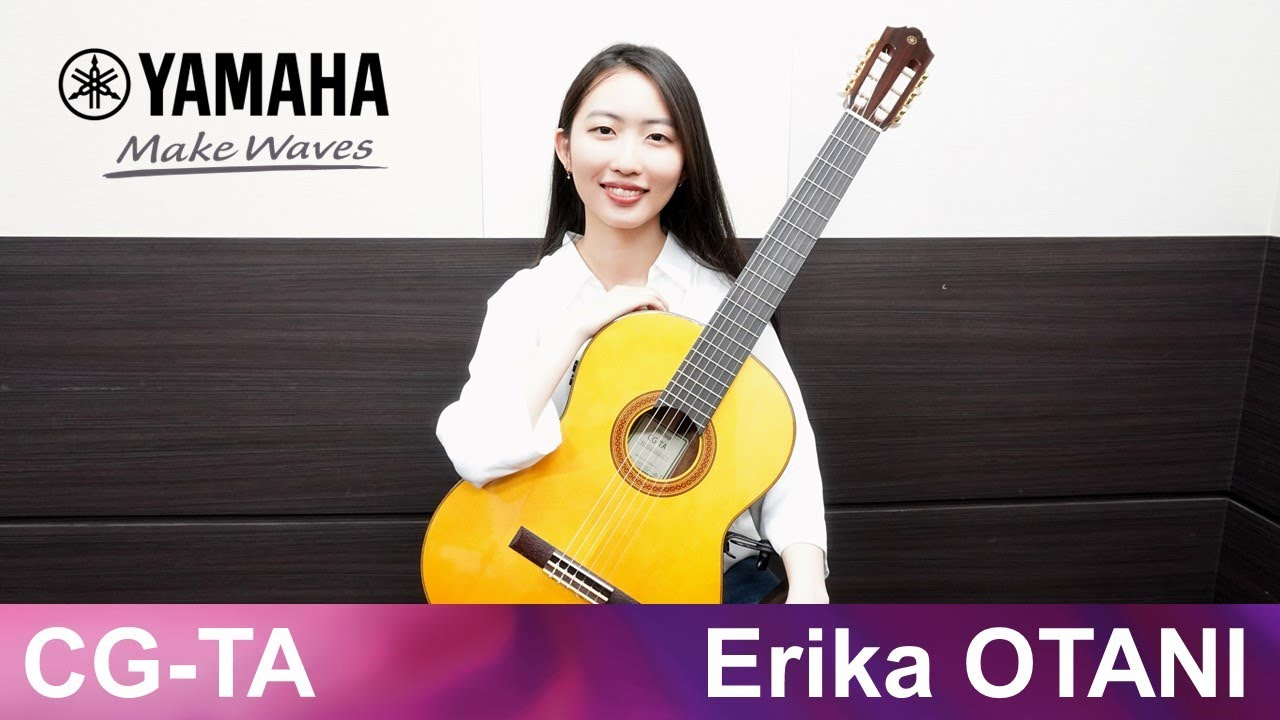
\includegraphics[width=0.48\linewidth]{pictures/youtube/2026/02/20260215_022157_youtube_002_qhMkWOjO0Qs.jpg}
}
\end{center}




私にはとてもこんなに指が動く様になれるとは思えないので、（素敵な曲ではあるけれども）演奏するのはハナから諦めている


この方の解説↓面白い

\url{https://youtu.be/7oEaIhpFFOM}

\begin{center}
\href{https://youtu.be/7oEaIhpFFOM}{
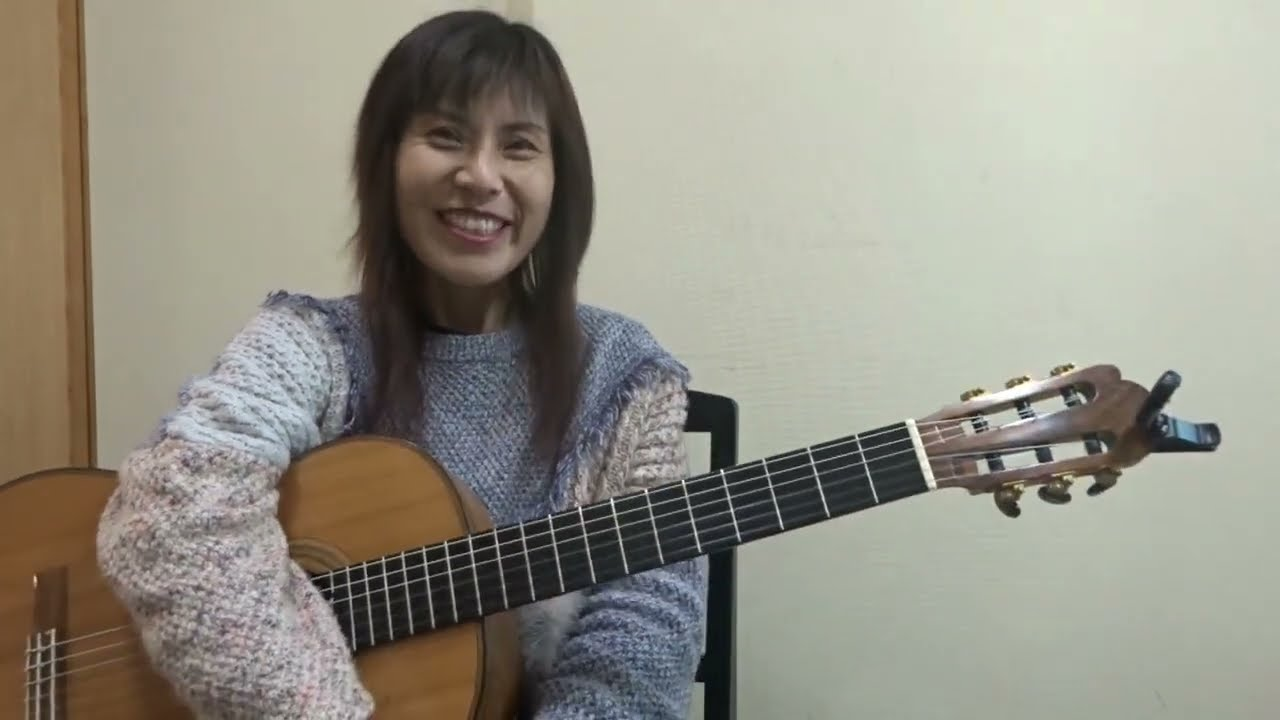
\includegraphics[width=0.48\linewidth]{pictures/youtube/2026/02/20260215_022157_youtube_003_7oEaIhpFFOM.jpg}
}
\end{center}




===

以下↓の記事の続きです

（お上手な方はたくさんいらっしゃる）

\url{https://www.facebook.com/100002225117991/posts/24477927645198066/}



\subsection*{2026年02月15日 02:24}
\addcontentsline{toc}{subsection}{2026年02月15日 02:24}

\paragraph{リンク}
\url{https://youtu.be/SbCDjfIVow0}

\begin{center}
\href{https://youtu.be/SbCDjfIVow0}{
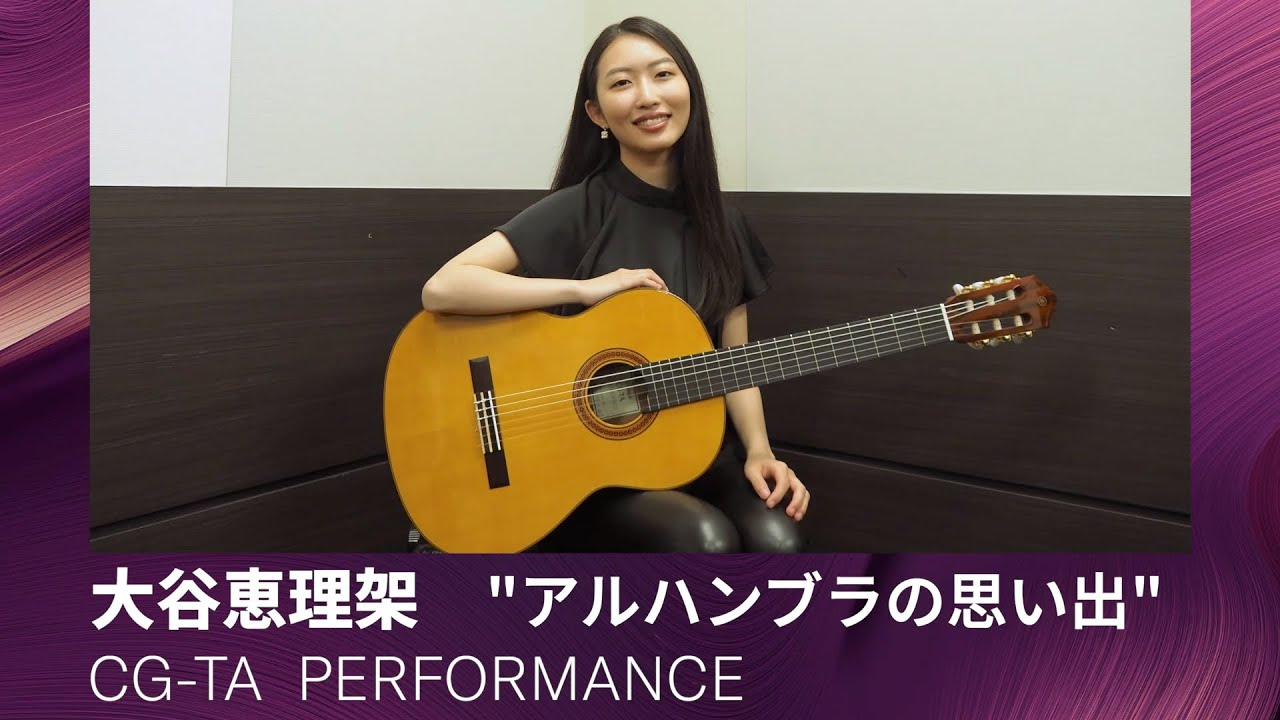
\includegraphics[width=0.48\linewidth]{pictures/youtube/2026/02/20260215_022403_youtube_001_SbCDjfIVow0.jpg}
}
\end{center}

\subsection*{2026年02月15日 11:28}
\addcontentsline{toc}{subsection}{2026年02月15日 11:28}

\paragraph{リンク}
\url{https://youtu.be/ZDtH98ClV3s}

\begin{center}
\href{https://youtu.be/ZDtH98ClV3s}{
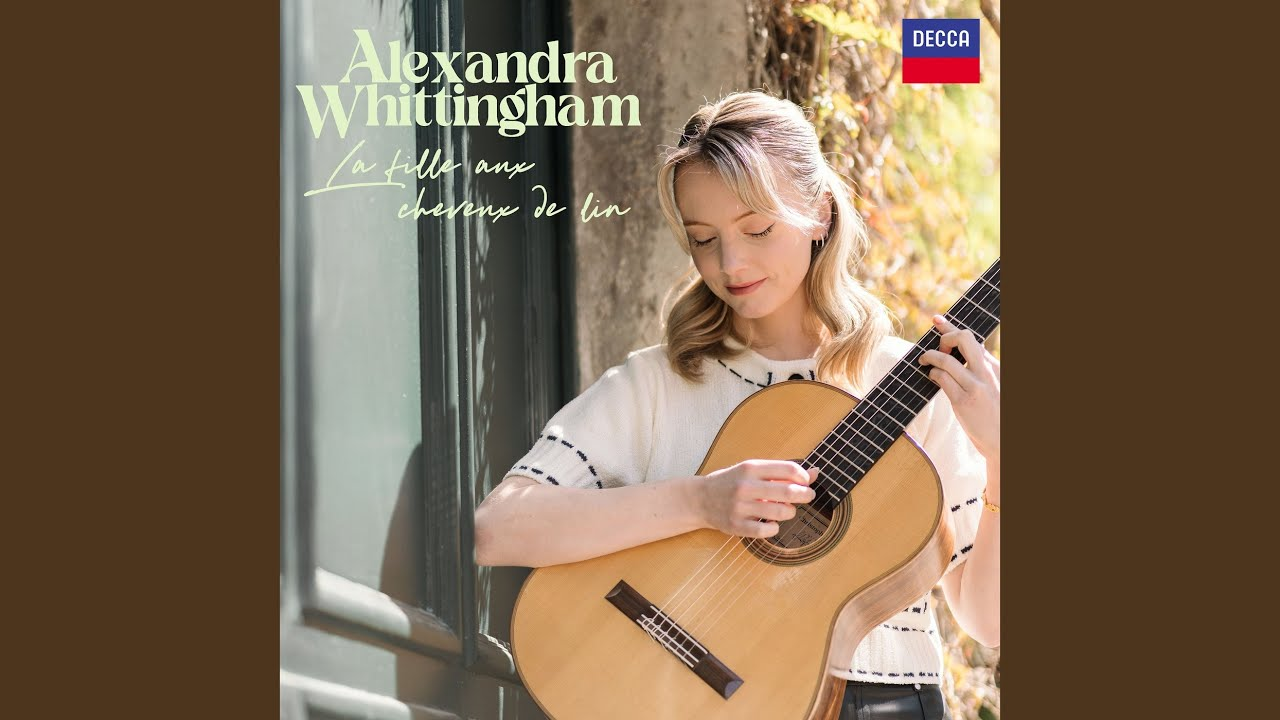
\includegraphics[width=0.48\linewidth]{pictures/youtube/2026/02/20260215_112839_youtube_001_ZDtH98ClV3s.jpg}
}
\end{center}

\subsection*{2026年02月15日 19:33}
\addcontentsline{toc}{subsection}{2026年02月15日 19:33}

愛の賛歌、歌っていたのはエディット ピアフ。

\url{https://youtu.be/gJKV7121-Qc}

\begin{center}
\href{https://youtu.be/gJKV7121-Qc}{
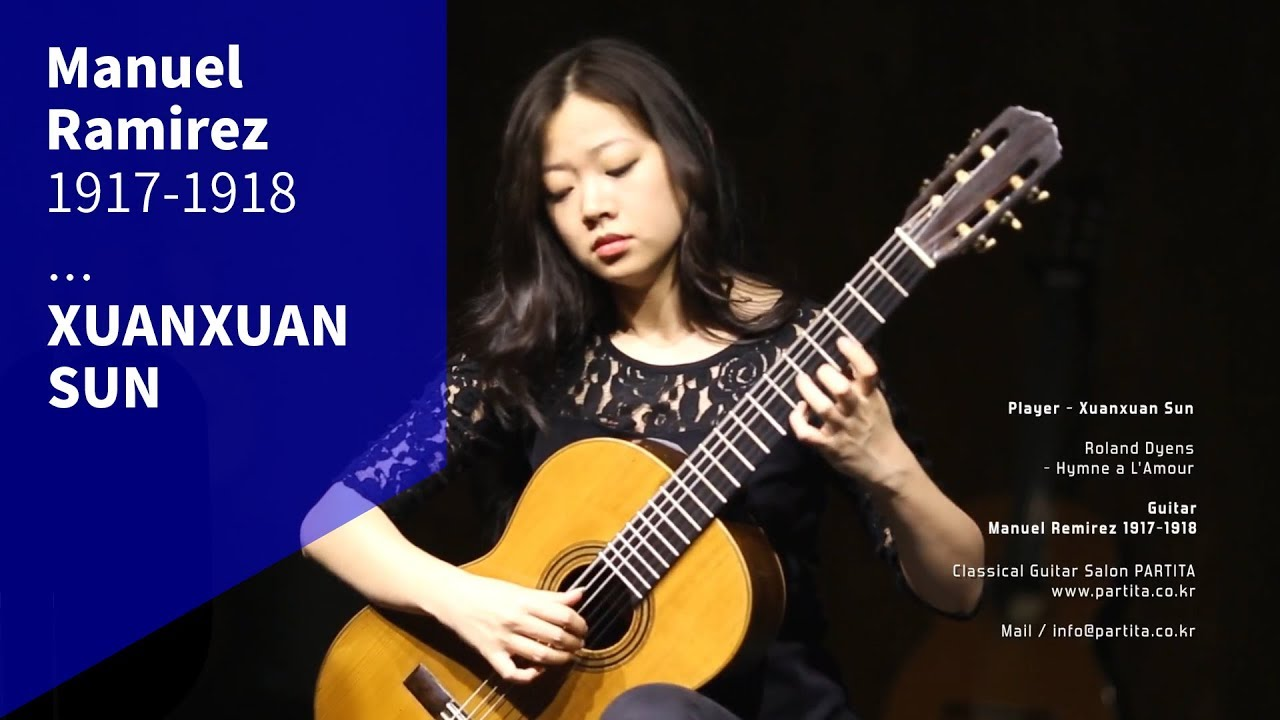
\includegraphics[width=0.48\linewidth]{pictures/youtube/2026/02/20260215_193305_youtube_001_gJKV7121-Qc.jpg}
}
\end{center}



\url{https://youtu.be/PGuWYNIguAQ}

\begin{center}
\href{https://youtu.be/PGuWYNIguAQ}{
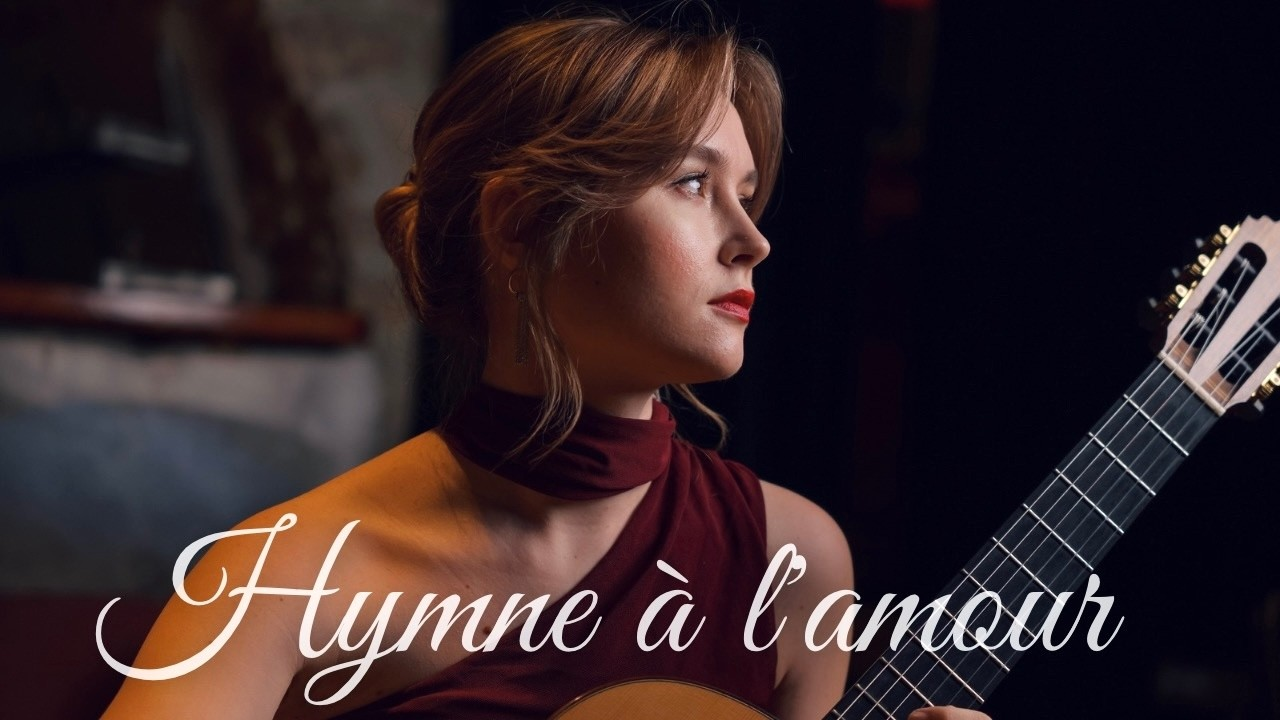
\includegraphics[width=0.48\linewidth]{pictures/youtube/2026/02/20260215_193305_youtube_002_PGuWYNIguAQ.jpg}
}
\end{center}




このギター編はRoland Dyens （ローラン・ディアンス）氏によるもの。

Dyens氏はM.Ravelの「亡き王女のためのパヴァーヌ」のギター編（ 

\url{https://www.facebook.com/share/1GaNkDYSBo/?mibextid=wwXIfr}

 ）も手掛けていらっしゃいますし、Over the Rainbowの編曲（ 

\url{https://www.facebook.com/reel/906127892326802/?fs=e&fs=e}

 ）もあります。

この愛の賛歌の編曲も、元々クラシック ギターのための曲ではなかったか、と紛うばかりの素晴らしい編曲だと思います（この編曲譜で演奏に挑戦したい所ですが、楽譜はどこに載っている？）。


ところで、そもそもの作曲者は誰？（↓）


===

「愛の讃歌」（仏: Hymne à l'amour）は、フランスのシャンソン歌手、エディット・ピアフの歌。作詞はピアフ、作曲はマルグリット・モノーによる。シャンソンを代表する楽曲として世界中で親しまれている。（Wikipediaより）

\subsection*{2026年02月17日 04:46}
\addcontentsline{toc}{subsection}{2026年02月17日 04:46}

\paragraph{リンク}
\url{https://youtu.be/N01fPgbXr-g}

\begin{center}
\href{https://youtu.be/N01fPgbXr-g}{
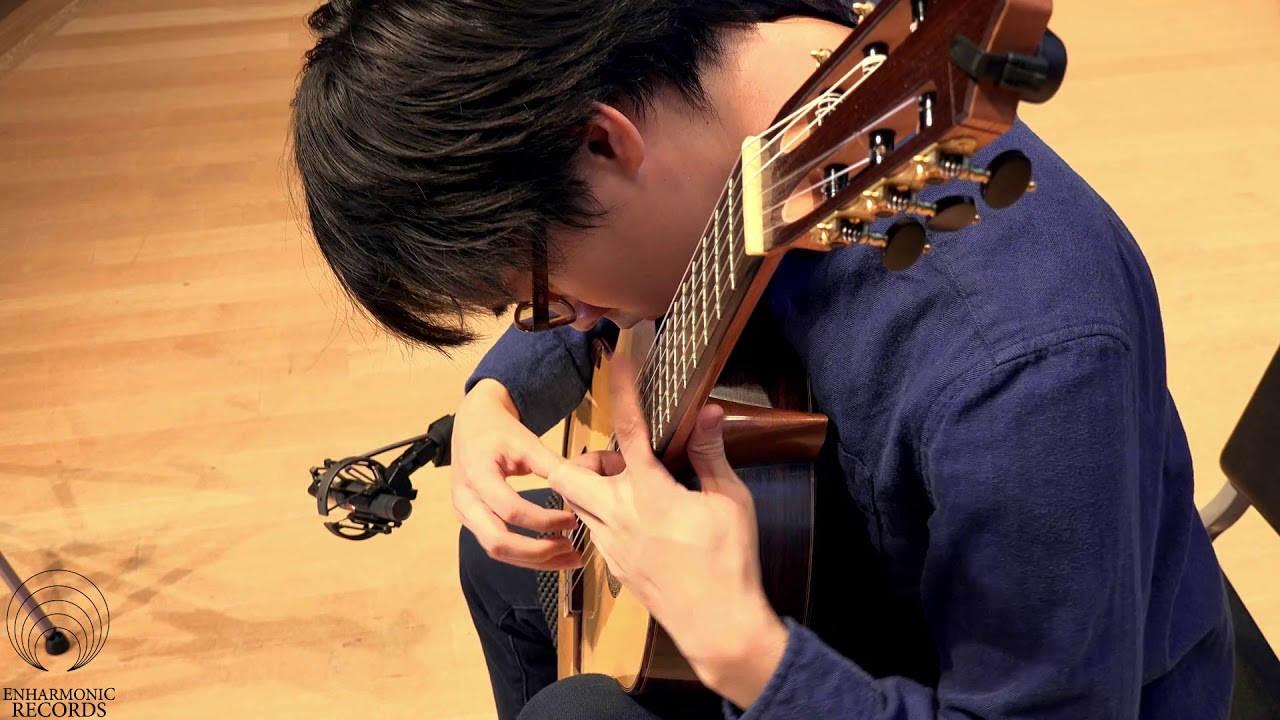
\includegraphics[width=0.48\linewidth]{pictures/youtube/2026/02/20260217_044632_youtube_001_N01fPgbXr-g.jpg}
}
\end{center}

\subsection*{2026年02月18日 19:42}
\addcontentsline{toc}{subsection}{2026年02月18日 19:42}

\url{https://youtu.be/tDbDmL9F6C8}

\begin{center}
\href{https://youtu.be/tDbDmL9F6C8}{
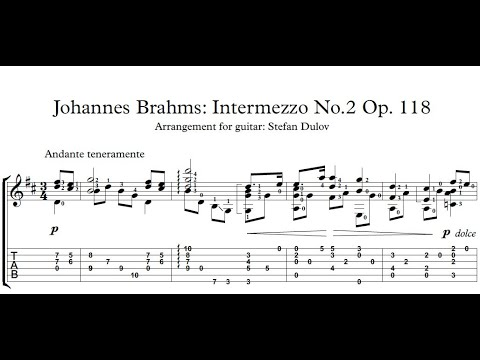
\includegraphics[width=0.48\linewidth]{pictures/youtube/2026/02/20260218_194207_youtube_001_tDbDmL9F6C8.jpg}
}
\end{center}



\subsection*{2026年02月19日 19:28}
\addcontentsline{toc}{subsection}{2026年02月19日 19:28}

本日（2月19日）金沢の月の入り（沈むところ）

赤→白→紫→青→黒 のグラデーションが美しい

（本物は写真よりずっと美しいんだけど、、）


月の下の白い点は水星かと思はれます

そのさらに下には金星がいるらしいのですが、もう地平線の下？いや、これは、、雲の合間の赤い点は、、、金星も写ってるんじゃない？


明日20日になると土星も月の下に現れるという事らしい

今日と同じ様に金星が写り込める時間帯には、月の位置はもっと上になるのか（色々厳しい撮影条件になりそうです）


\url{https://www.nao.ac.jp/astro/sky/2026/02-topics02.html}



\paragraph{写真}
\begin{center}
\begin{minipage}{0.48\linewidth}
\centering
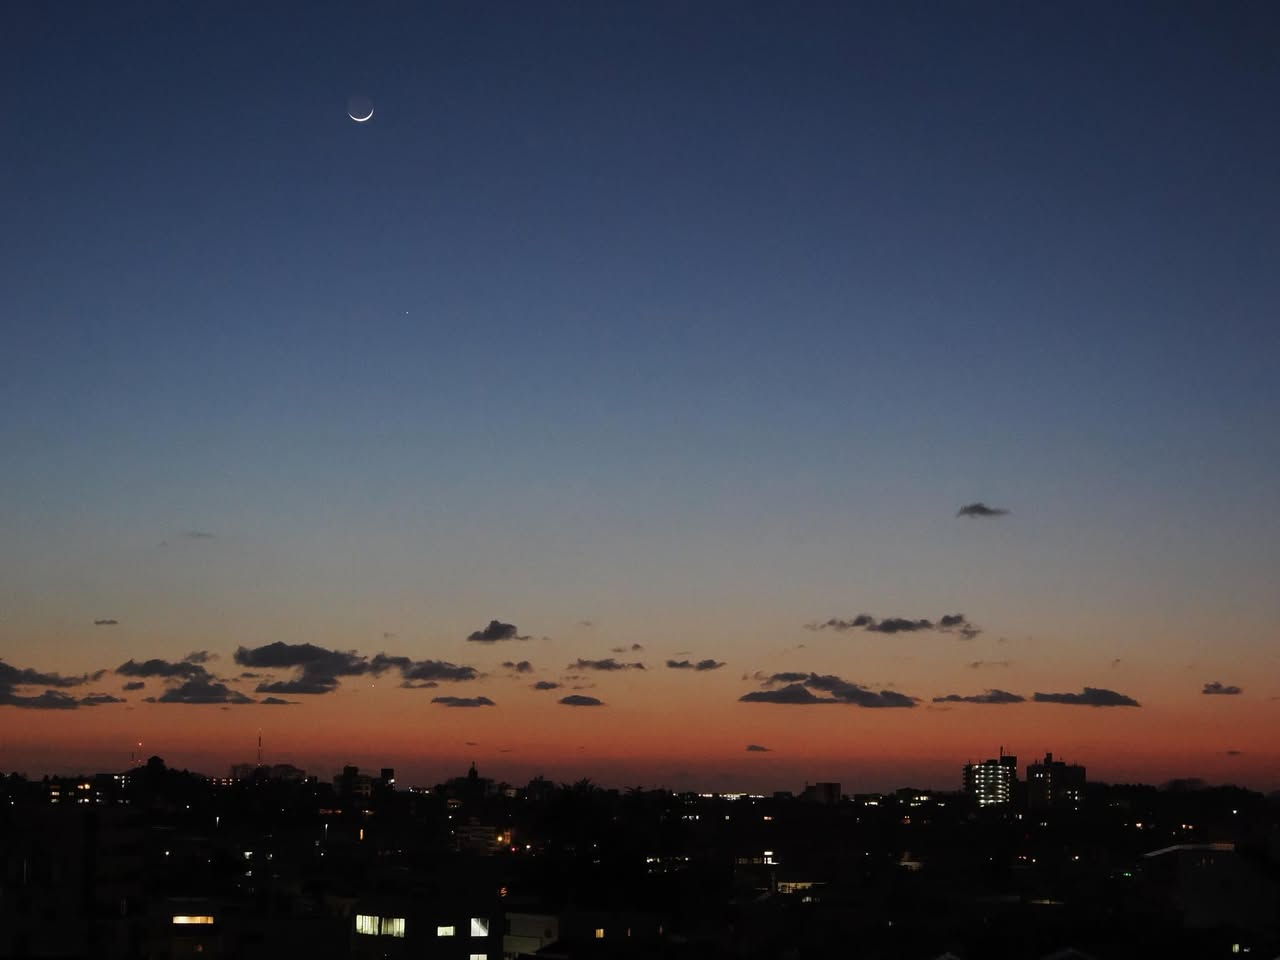
\includegraphics[width=\linewidth]{pictures/2026/02/20260219_192816_001.jpg}
\end{minipage}
\hfill
\begin{minipage}{0.48\linewidth}
\centering
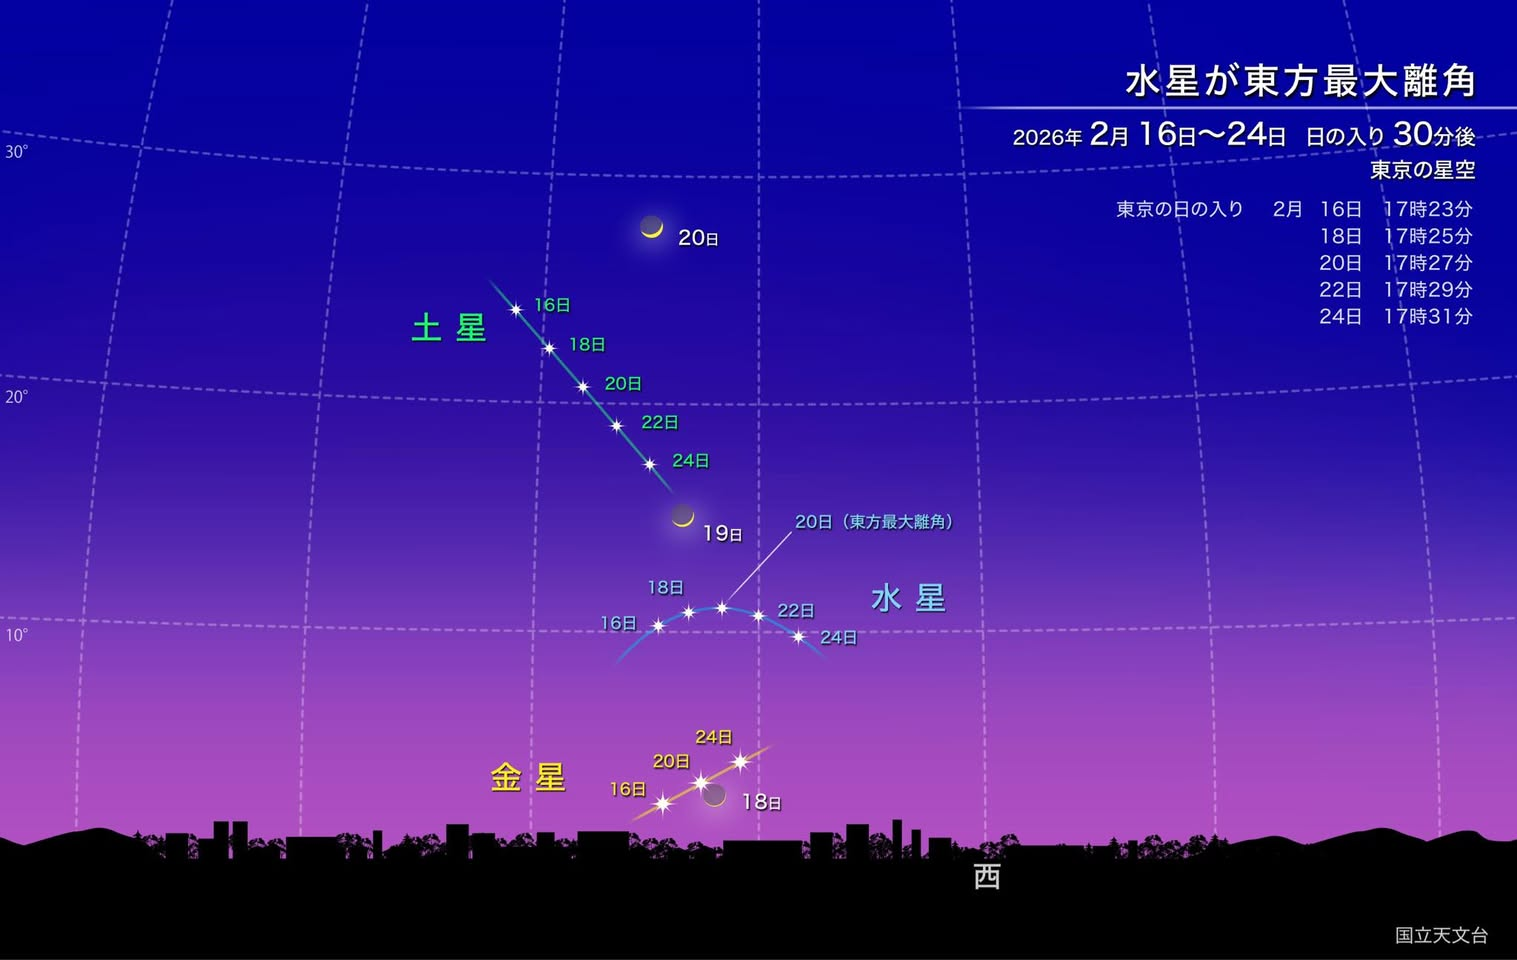
\includegraphics[width=\linewidth]{pictures/2026/02/20260219_192816_002.jpg}
\end{minipage}
\end{center}

\subsection*{2026年02月20日 05:54}
\addcontentsline{toc}{subsection}{2026年02月20日 05:54}

\paragraph{リンク}
\url{https://youtu.be/11o-6Gr6M48}

\begin{center}
\href{https://youtu.be/11o-6Gr6M48}{
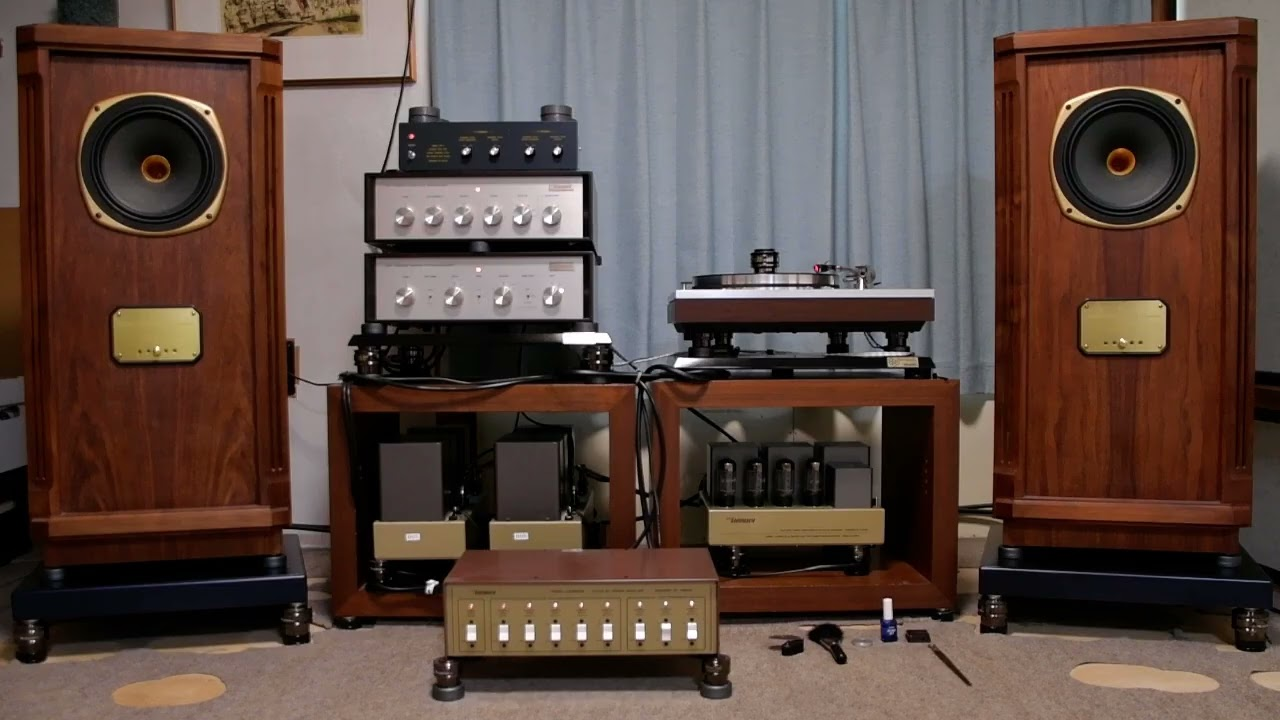
\includegraphics[width=0.48\linewidth]{pictures/youtube/2026/02/20260220_055433_youtube_001_11o-6Gr6M48.jpg}
}
\end{center}

\subsection*{2026年02月20日 09:09}
\addcontentsline{toc}{subsection}{2026年02月20日 09:09}

大きな期待がかけられている国家プロジェクトでもあるんですよね。ある程度のレベルの「お湯を沸かす」ために解決しなければならない（しかもbreak throughを要する様な）問題が複数横たわっているのではないか、と推察しています。


そもそもbreak throughとは（私の理解では）、解決への「道筋が見えていない」時の希望的な（仮想の）解決策の事で、いつ起きるか分からないし、起きるかどうかも分からない。


そんな中で、目標とする日程だけは（どうしても）設定されていく。しかも国際的な競争の只中にもいるため、かなり「前のめりの期限」で尻を叩かれている。尻を叩けば問題解決に結びつくヒラメキ、発見が現れるとも思えないけど、少なくとも税金で活動している以上は、どうしても必要になってくる事なのでしょう、、、厳しいですね。


それでも添付↓にある「現場」では、地道で根気強い研究開発の活動が日々行われていることと推察します。期待していますし、（気持ちだけですが）応援しています。


\url{https://x.com/nakaqst/status/2024318019002864105?s=61&t=5VtsOkpki6juEjPXsBq8hg}




===

以下の記事の続きです


\url{https://m.facebook.com/story.php?story_fbid=9110134879070592&id=100002225117991}



\paragraph{写真}
\begin{center}
\begin{minipage}{0.48\linewidth}
\centering
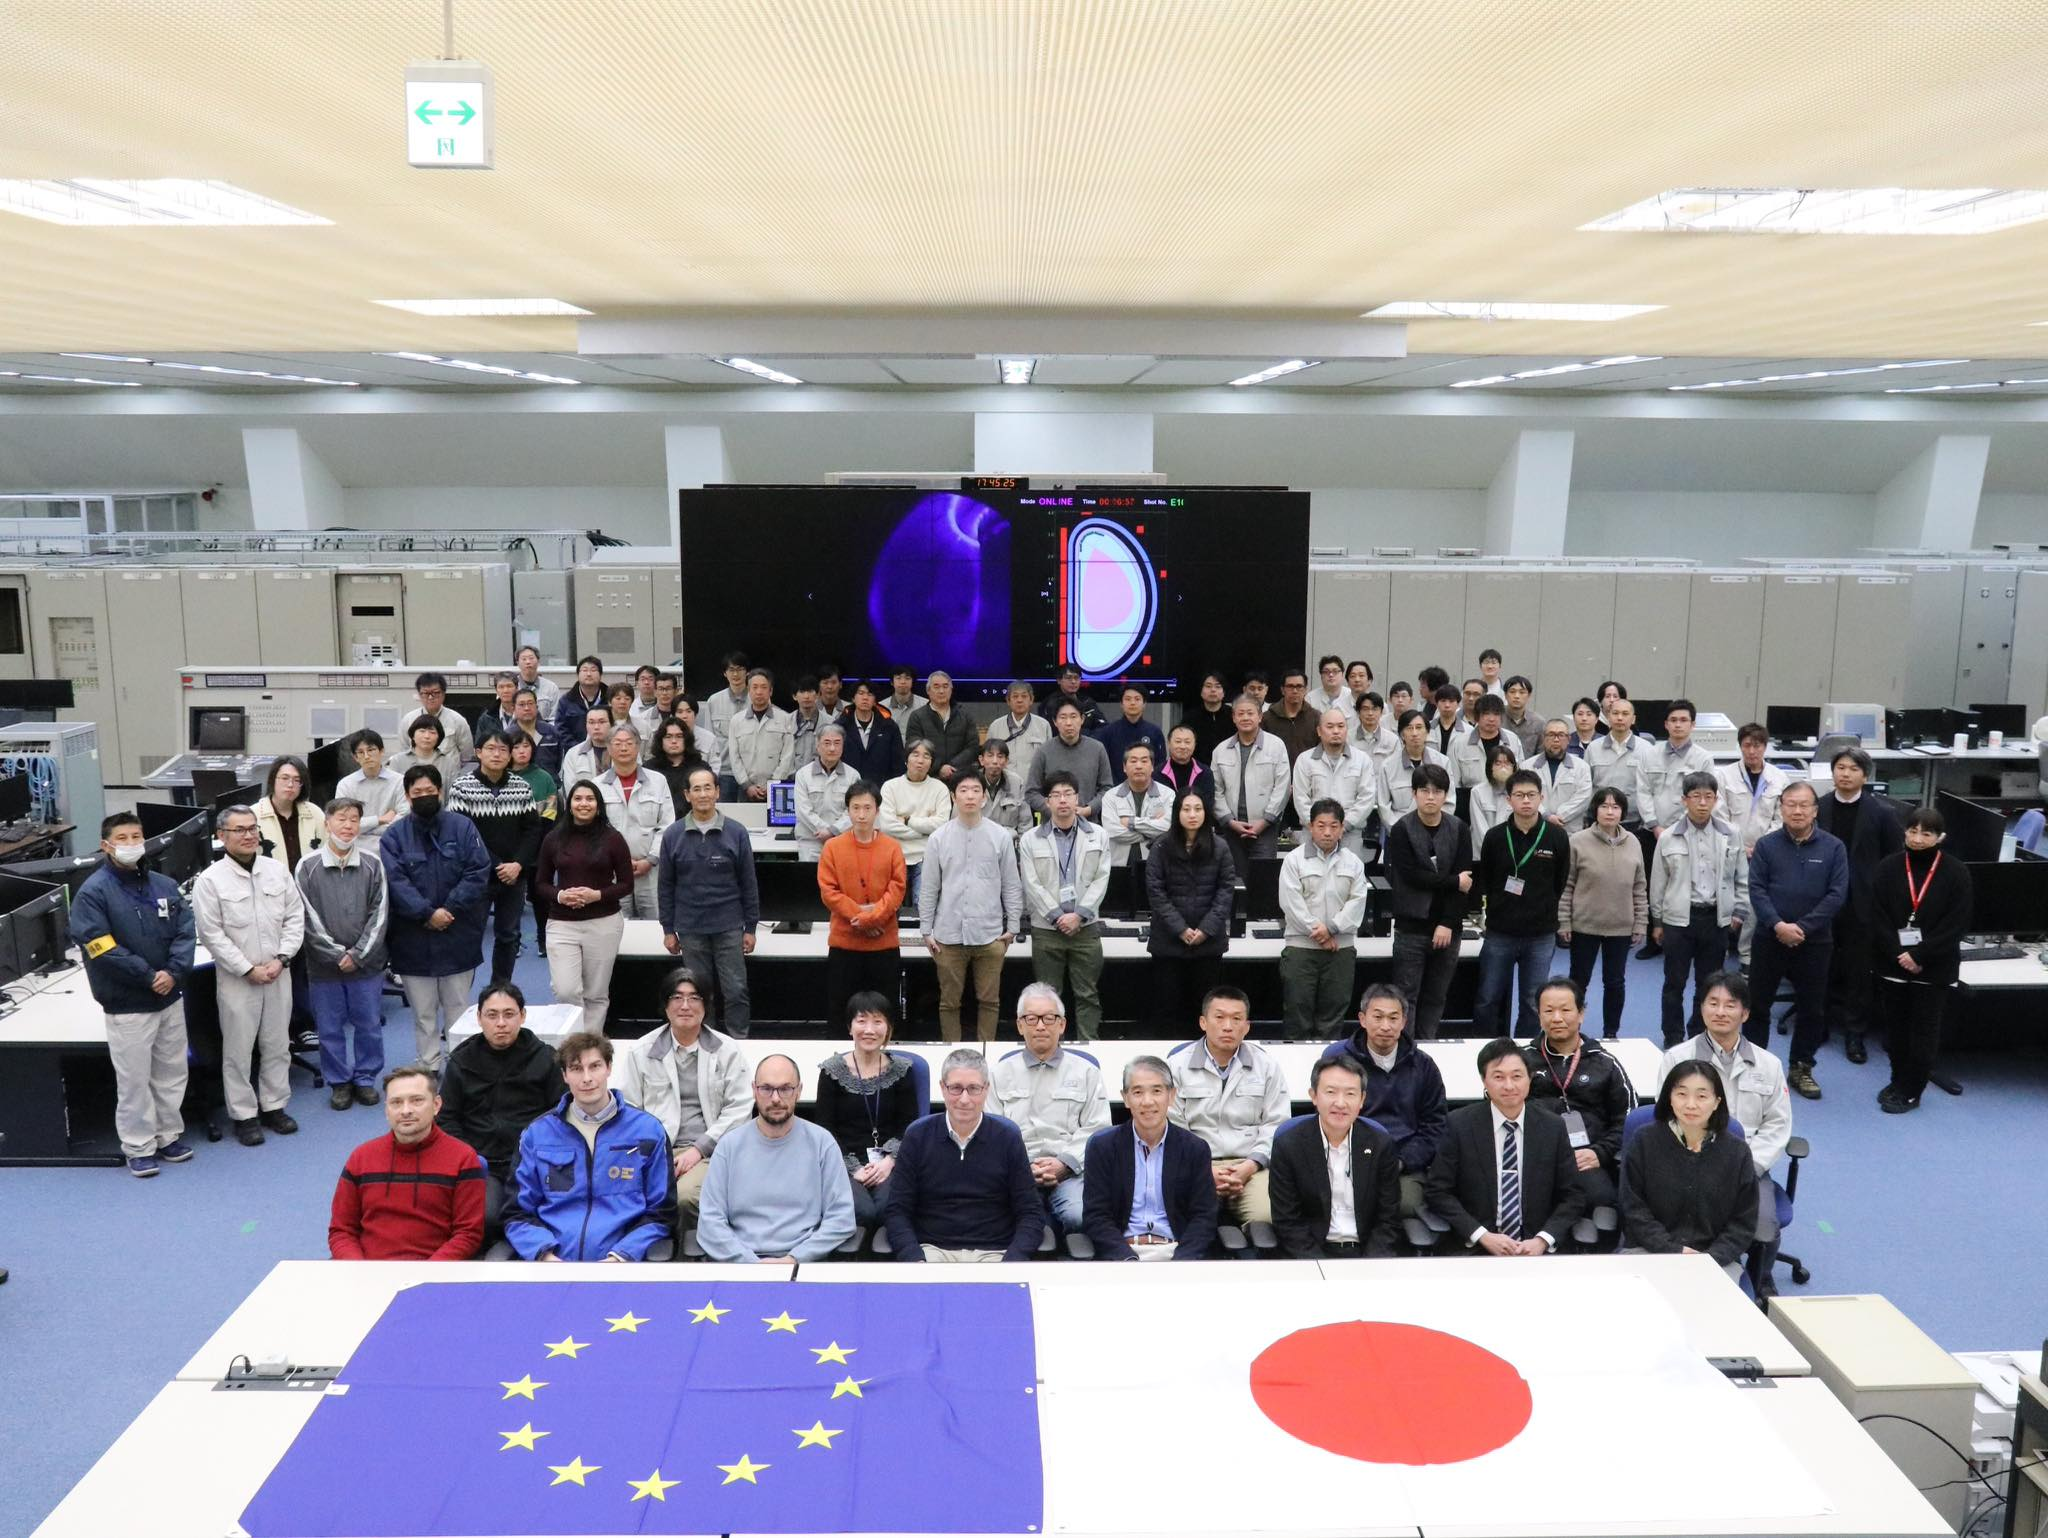
\includegraphics[width=\linewidth]{pictures/2026/02/20260220_090932_001.jpg}
\end{minipage}
\end{center}

\subsection*{2026年02月21日 19:54}
\addcontentsline{toc}{subsection}{2026年02月21日 19:54}

2月21日金沢の夕刻です

月ー土星ー水星ー金星

見えますか？（画面のゴミをよく拭いて、真剣に探さないと見つからんよ）

水星は灼熱地獄でしょうか？そして土星は極寒地獄でしょうか？


雲一つないので、今日は絶対に写せると思ってカメラを構えましたが、肉眼ではかなり高い位置に月が見えただけで、それ以外何も見えませんでした。空は思いの外明るかったということかも。一応タイムラプスで撮ってみてはいましたが、月の位置もとても高いので、月と地平線を同一画面に入れようと思うと、かなり広角にしないといけないし、こんな状態で惑星達が写るなどとは思っていませんでした。でも撮影後のデータをじっくり見ていたところ、、、土星も含めて、写っていたみたいです。（ウフウフうふふ）もう少し露光量増やした方がいいかも。月はこの場合もっと露出オーバーでもOkでしょうから。


海王星が土星の裏あたりにいる様ですが、暗くて小さいのでこの様な広角レンズのカメラでは写らないのでしょうね

28日には木星が月の近くに見えるみたいです（木星は大きいらしい）

\url{https://starwalk.space/ja/news/planetary-alignment-february-28-2026}




===

以下の記事の続きです


\url{https://m.facebook.com/story.php?story_fbid=25859069360417214&id=100002225117991}



\paragraph{写真}
\begin{center}
\begin{minipage}{0.48\linewidth}
\centering
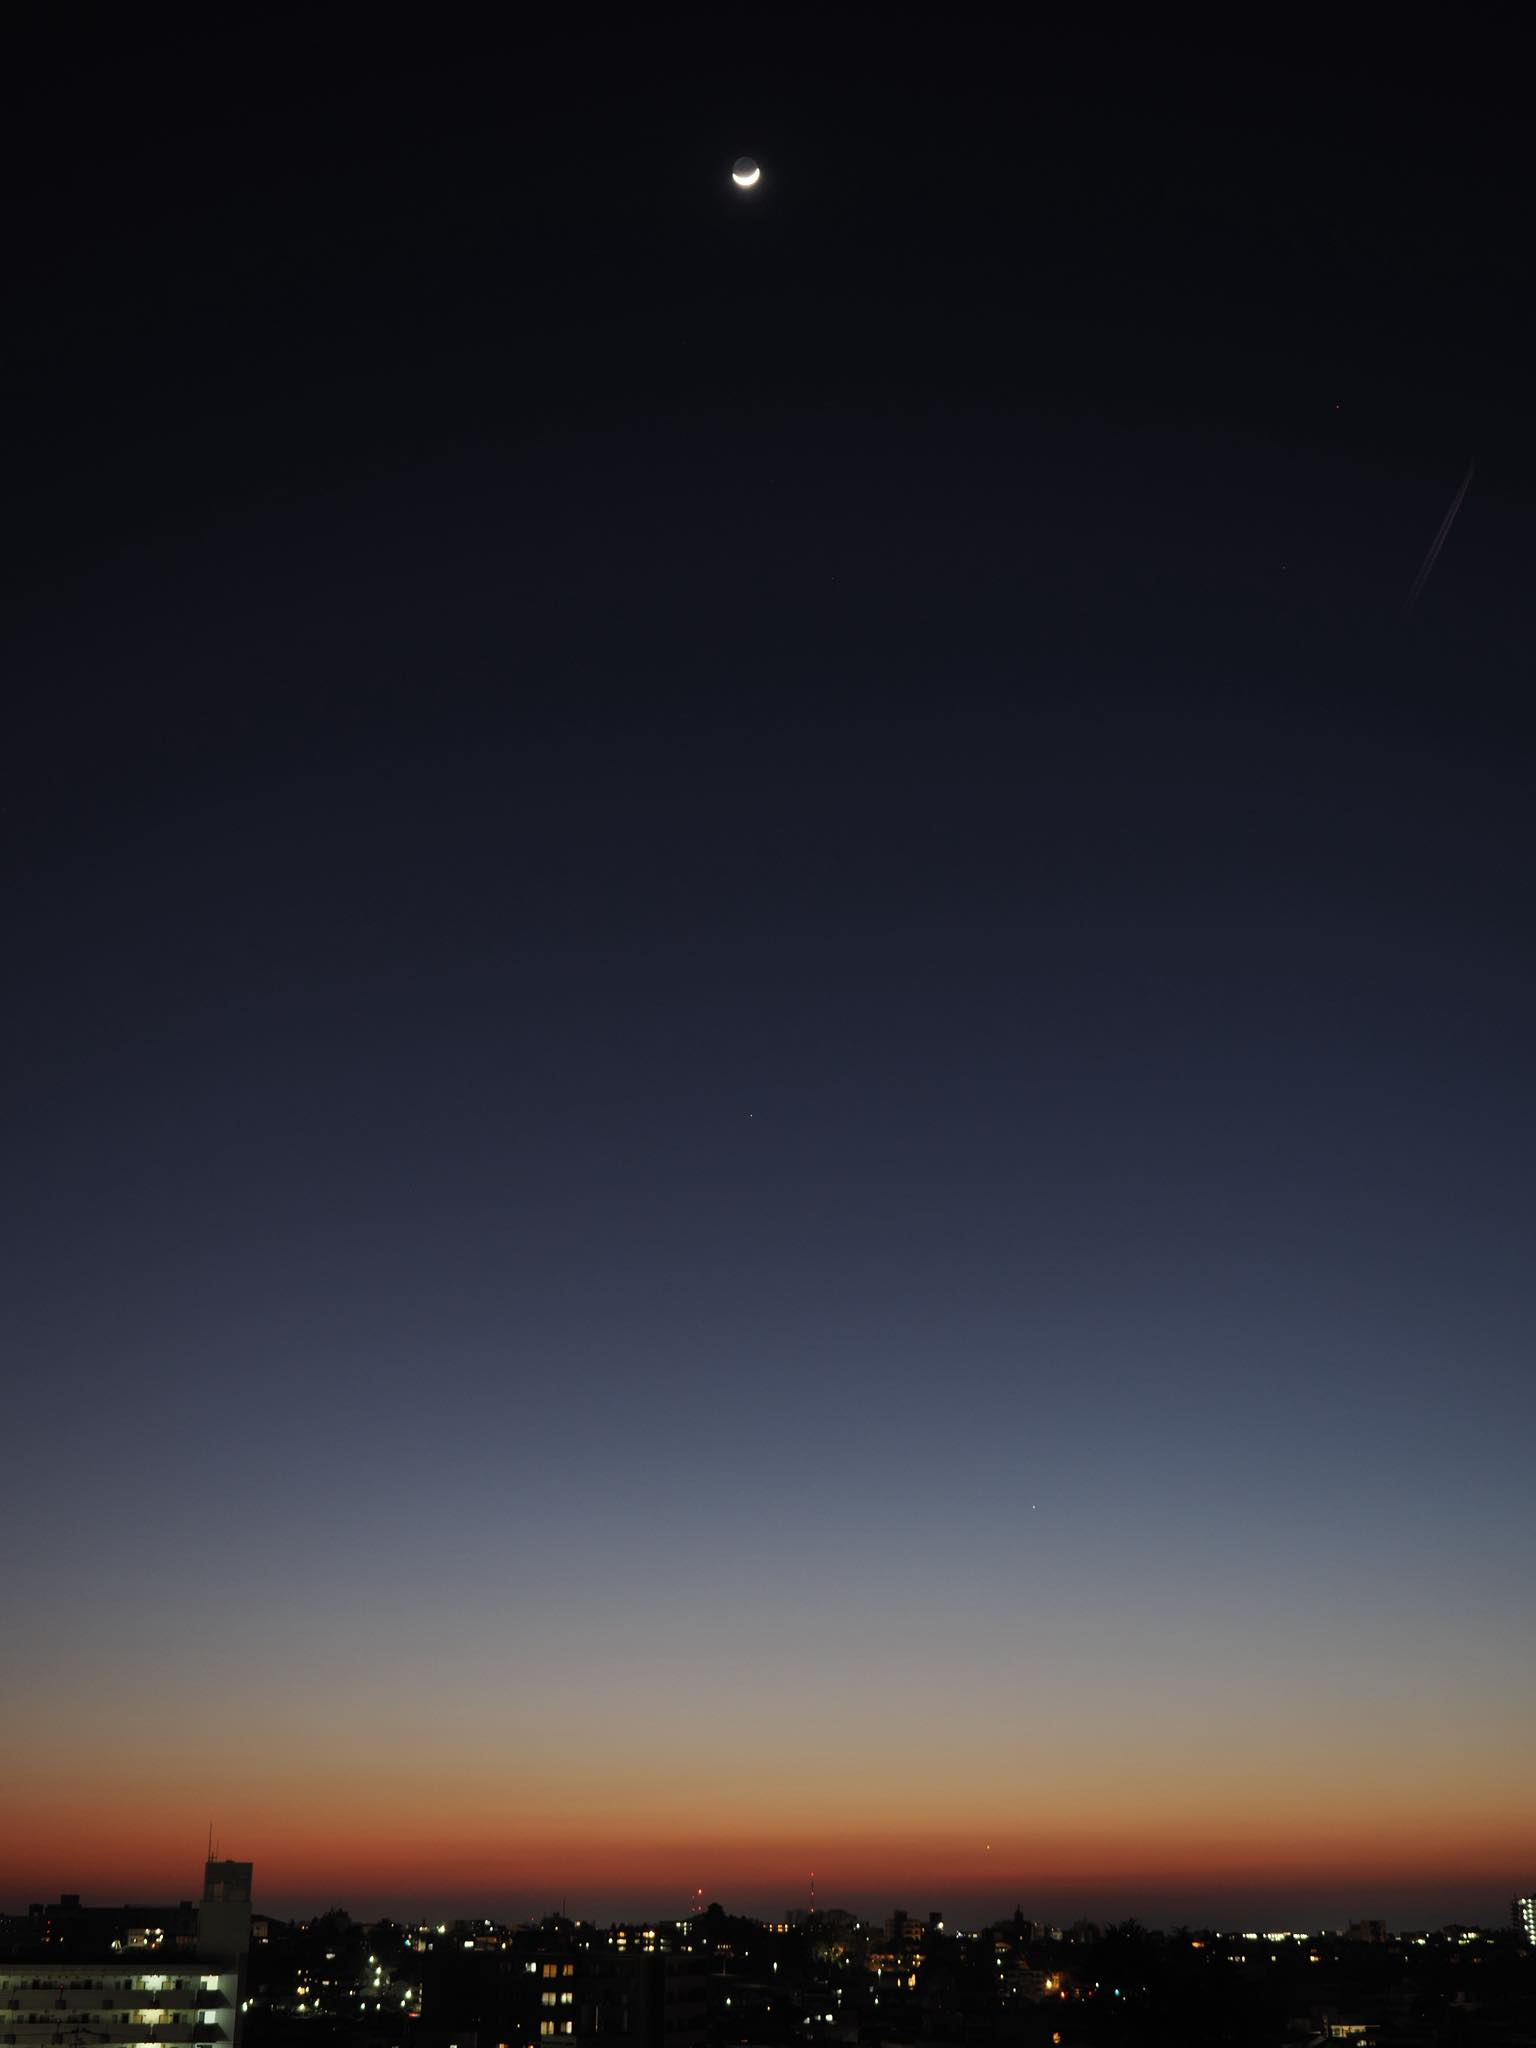
\includegraphics[width=\linewidth]{pictures/2026/02/20260221_195409_001.jpg}
\end{minipage}
\end{center}

\subsection*{2026年02月22日 21:10}
\addcontentsline{toc}{subsection}{2026年02月22日 21:10}

オシャレな曲のオシャレな編曲とその演奏

（武満徹のギターのための曲はみんなオシャレなんだけど別扱いとして）

以下のギター編曲譜はおおかた入手済み（ 後は演奏するばかりだが(-｡-; ）


(１)Smoke Gets in Your Eyes（J.W.Duarte編）

\url{https://www.facebook.com/100002225117991/posts/10029604293790308/}




(２)Over the Rainbow（David Jaggs編）

\url{https://www.facebook.com/100002225117991/posts/9464987030252040/}




(３)愛の讃歌（Roland Dyens編）

\url{https://www.facebook.com/100002225117991/posts/25822762094047941/}




(４)What a Wonderful World（鈴木大介編）

\url{https://www.facebook.com/100002225117991/posts/9945968618820543/}




(５)Waltz for Debby（Greg Stone編）

\url{https://m.facebook.com/story.php?story_fbid=24451524207838410&id=100002225117991}




(６)My Way（青木一男編）

\url{https://www.facebook.com/100002225117991/posts/23888974657426704/}




(７)エストレリータ（ホセ・ルイス・ゴンザレス編）

\url{https://www.facebook.com/100002225117991/posts/9484462508304492/}




(８)パリの空の下（竹内永和編）

\url{https://www.facebook.com/100002225117991/posts/25906538289003654/}




(９)ララルー（江部賢一編）

\url{https://www.facebook.com/100002225117991/posts/26083319101325571/}




(10) ピンクパンサー（楽譜欲しい）

\url{https://x.com/old_but_gold50s/status/2042384563712749989?s=61&t=5VtsOkpki6juEjPXsBq8hg}




(１１) これは？

\url{https://www.facebook.com/reel/1196932181977051/?fs=e&fs=e}




(１２)

\url{https://youtu.be/3dLbZDPL0Eg}

\begin{center}
\href{https://youtu.be/3dLbZDPL0Eg}{
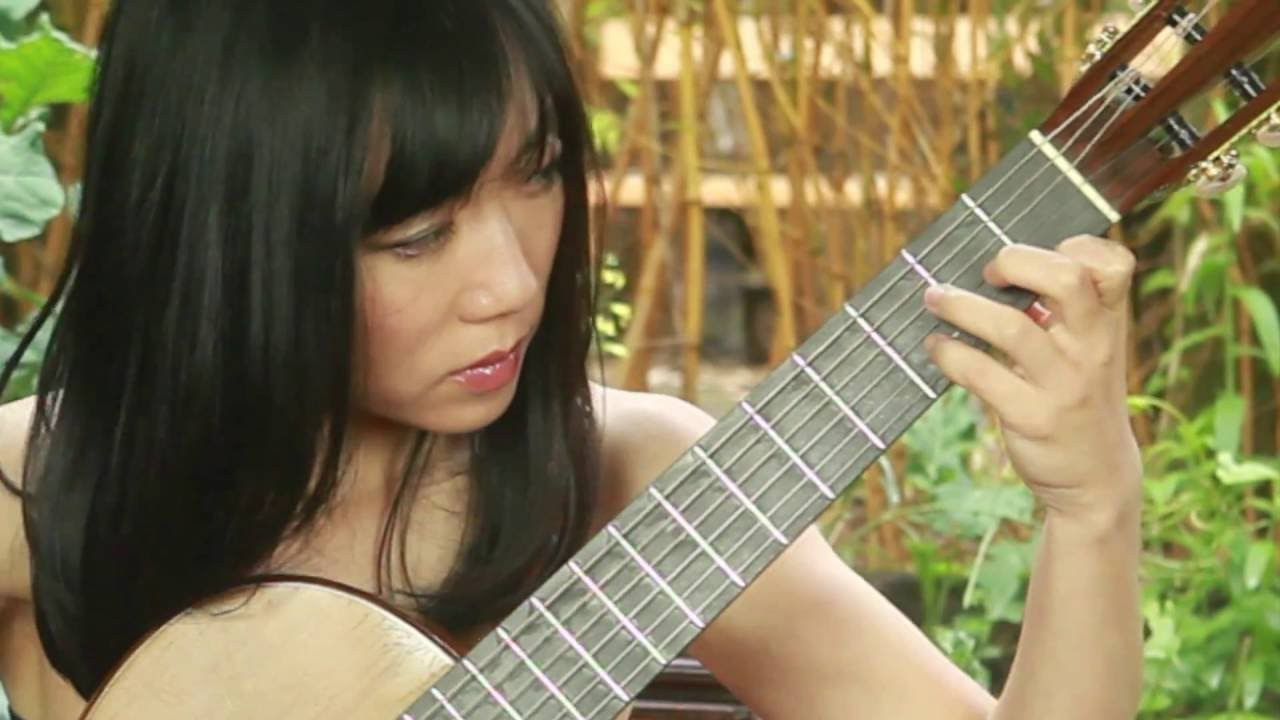
\includegraphics[width=0.48\linewidth]{pictures/youtube/2026/02/20260222_211006_youtube_001_3dLbZDPL0Eg.jpg}
}
\end{center}




＊こうやって曲のリンクをリストに集めてみると、これらの曲を貫く（共通する）もの、自分がお洒落だと感じているもの、とは何なんだろうか？と考えてしまいます。それは万人が素敵だと感じているものと同じものなのか？それは大衆的でポピュラーな曲であれば通常備えているであろう特徴そのものなのか？しかし、他の人が集めたリンク集が別途あるとすれば、それにはおそらく自分の入れたくない曲も含まれることでしょう。10人いれば10通りのリストができる事でしょう。そうであればやはり、自分が素敵だと思っているものとはいったい何なんだろう。自分がリンクのリストに加えるか加えないかの判断基準にしているものは何なのか？など、など、そんな事をあれこれ思いを巡らせています。

\subsection*{2026年02月23日 08:38}
\addcontentsline{toc}{subsection}{2026年02月23日 08:38}

\paragraph{リンク}
\url{https://youtu.be/zRGOKd2DmM0}

\begin{center}
\href{https://youtu.be/zRGOKd2DmM0}{
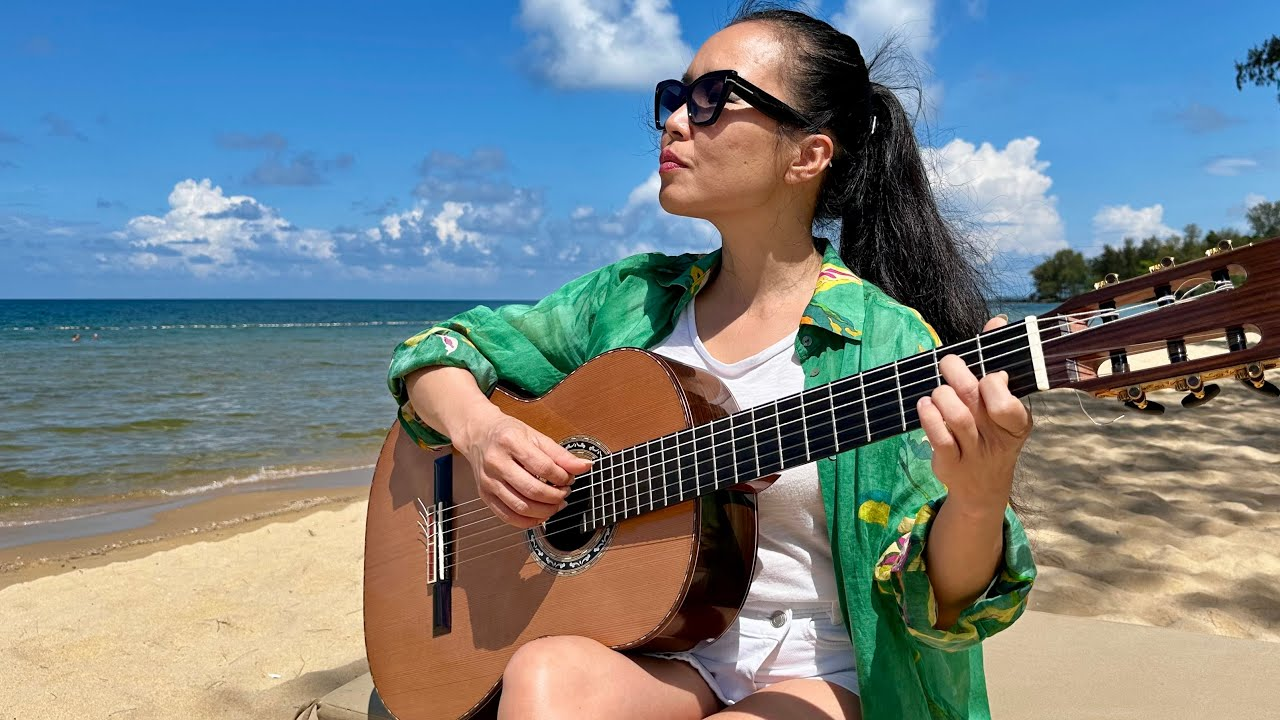
\includegraphics[width=0.48\linewidth]{pictures/youtube/2026/02/20260223_083810_youtube_001_zRGOKd2DmM0.jpg}
}
\end{center}

\subsection*{2026年02月23日 08:49}
\addcontentsline{toc}{subsection}{2026年02月23日 08:49}

\paragraph{リンク}
\url{https://youtu.be/hrsFr48-MYg}

\begin{center}
\href{https://youtu.be/hrsFr48-MYg}{
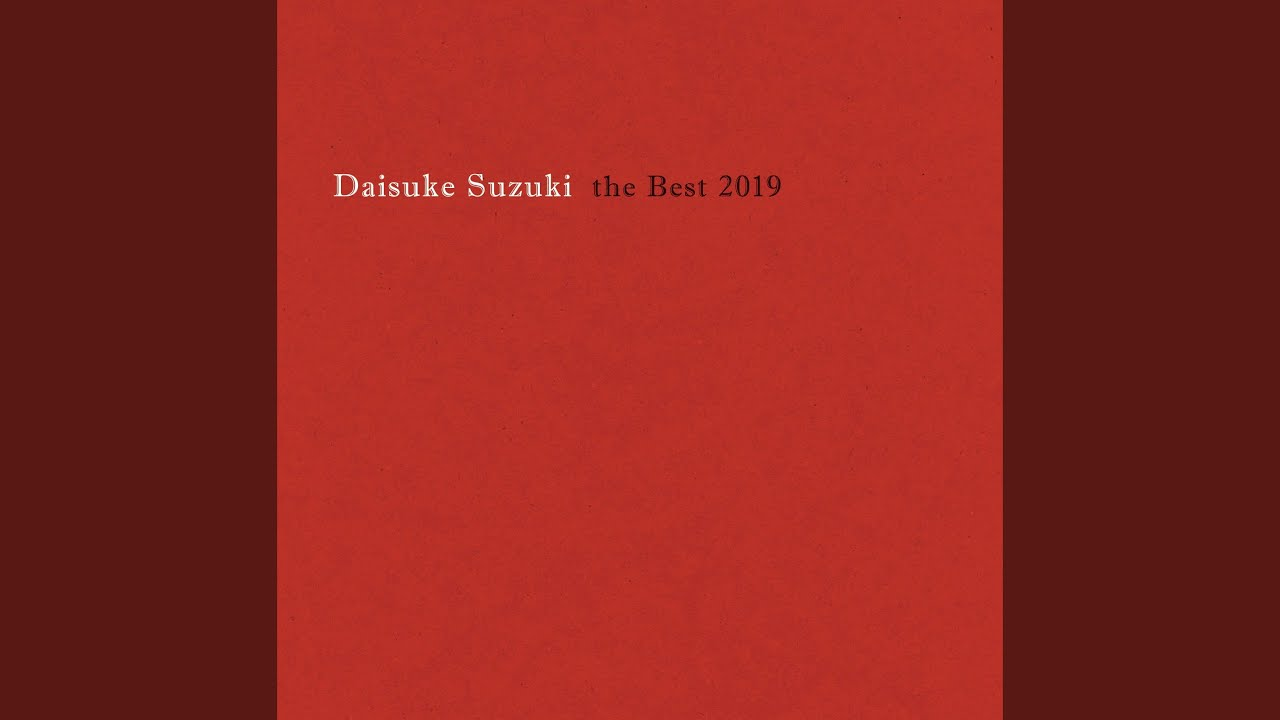
\includegraphics[width=0.48\linewidth]{pictures/youtube/2026/02/20260223_084934_youtube_001_hrsFr48-MYg.jpg}
}
\end{center}

\subsection*{2026年02月23日 08:50}
\addcontentsline{toc}{subsection}{2026年02月23日 08:50}

\paragraph{リンク}
\url{https://youtu.be/CaCSuzR4DwM}

\begin{center}
\href{https://youtu.be/CaCSuzR4DwM}{
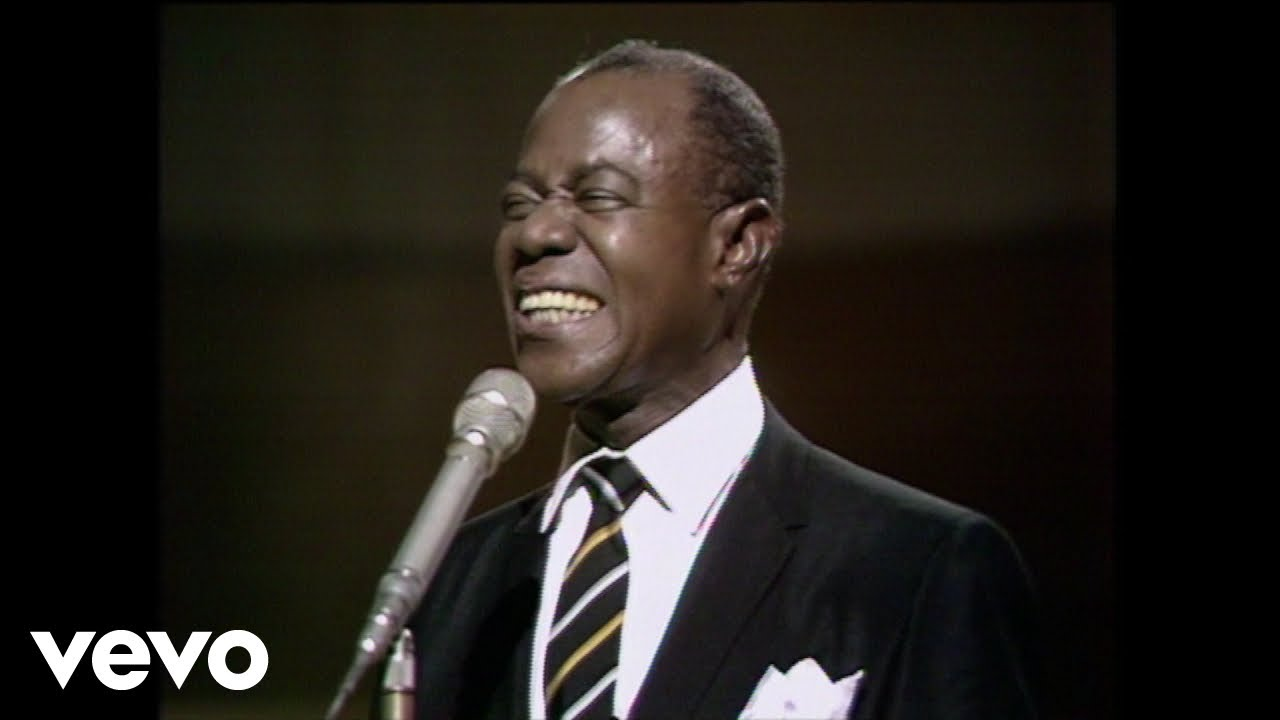
\includegraphics[width=0.48\linewidth]{pictures/youtube/2026/02/20260223_085027_youtube_001_CaCSuzR4DwM.jpg}
}
\end{center}

\subsection*{2026年02月23日 09:37}
\addcontentsline{toc}{subsection}{2026年02月23日 09:37}

\paragraph{リンク}
\url{https://youtu.be/atMCC-_6xjk}

\begin{center}
\href{https://youtu.be/atMCC-_6xjk}{
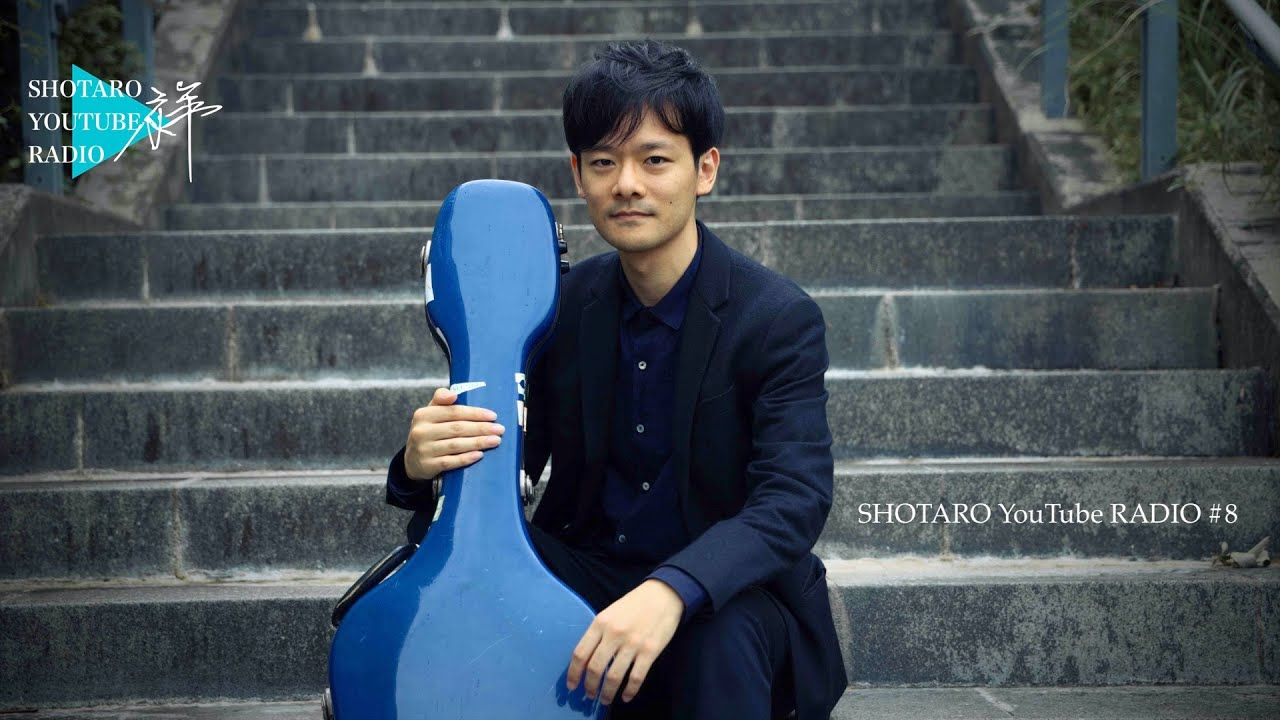
\includegraphics[width=0.48\linewidth]{pictures/youtube/2026/02/20260223_093723_youtube_001_atMCC-_6xjk.jpg}
}
\end{center}

\subsection*{2026年02月23日 09:43}
\addcontentsline{toc}{subsection}{2026年02月23日 09:43}

\paragraph{リンク}
\url{https://youtu.be/KadnVRvO4cM}

\begin{center}
\href{https://youtu.be/KadnVRvO4cM}{
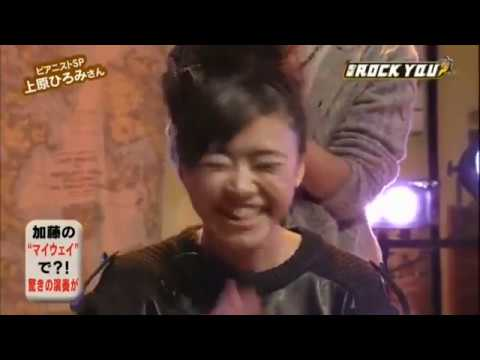
\includegraphics[width=0.48\linewidth]{pictures/youtube/2026/02/20260223_094357_youtube_001_KadnVRvO4cM.jpg}
}
\end{center}

\subsection*{2026年02月23日 20:35}
\addcontentsline{toc}{subsection}{2026年02月23日 20:35}

昭和47年とは、中学生の頃かな。懐かしい。

\url{https://youtu.be/k19WnZyfgBE}

\begin{center}
\href{https://youtu.be/k19WnZyfgBE}{
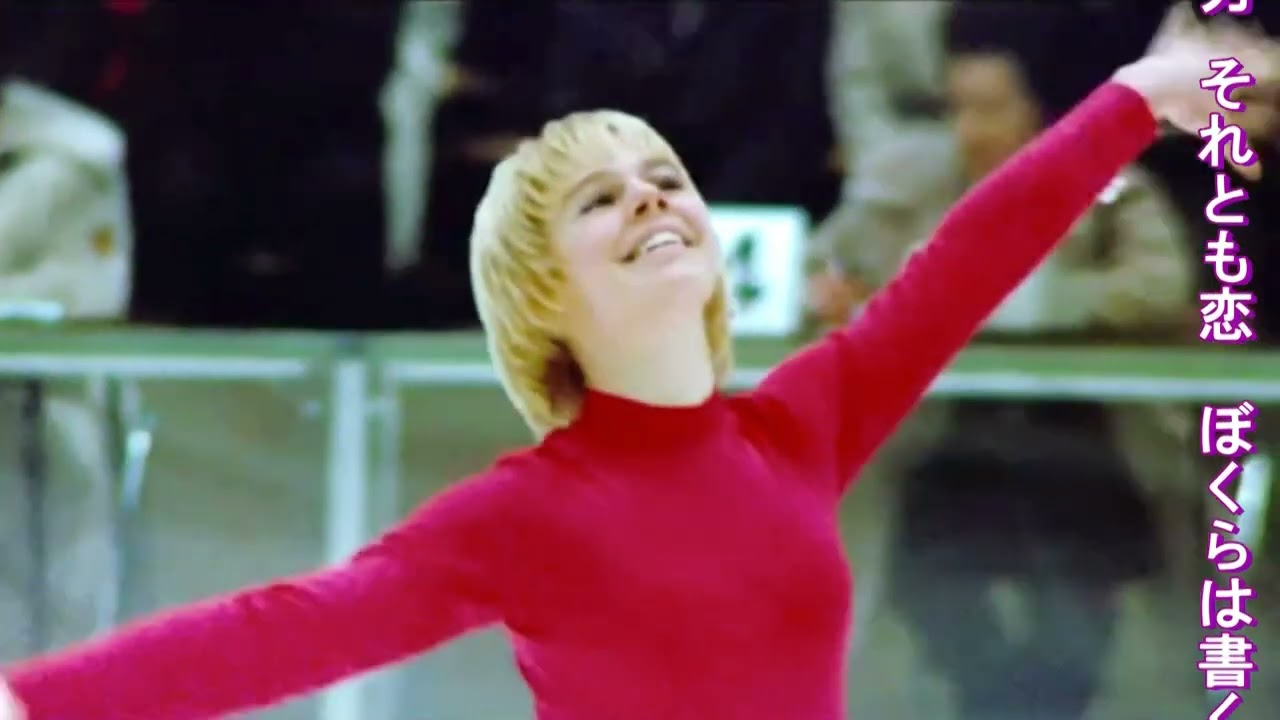
\includegraphics[width=0.48\linewidth]{pictures/youtube/2026/02/20260223_203518_youtube_001_k19WnZyfgBE.jpg}
}
\end{center}



\subsection*{2026年02月24日 22:52}
\addcontentsline{toc}{subsection}{2026年02月24日 22:52}

魅力的な選曲だなぁ

展覧会の絵を聞きたいな

Prelude, Fugue, Allegroも演奏される様だし

（※エッ、会場は和歌山県ですか？）

CD出して欲しいです（YouTubeでもいいです）


\url{https://m.facebook.com/events/2060624534484800/}




\url{https://www.facebook.com/photo.php?fbid=3143441632504556&set=a.188101438038605&type=3}




\url{https://m.facebook.com/story.php?story_fbid=3212649728917079&id=100005162491303}



\subsection*{2026年02月24日 23:11}
\addcontentsline{toc}{subsection}{2026年02月24日 23:11}

竹内永和編「ポピュラーギター傑作選Vol.1」現代ギター社刊（ 

\url{https://www.gendaiguitar.com/products/4539442061707}

 ）でしょうか？


低音で、ズンチャッチャッ、ズンチャッチャッ、とリズムをとっているのは、如何にも下町の大衆音楽っぽい雰囲気を醸し出しています

\url{https://youtu.be/OErGrh18mCg}

\begin{center}
\href{https://youtu.be/OErGrh18mCg}{
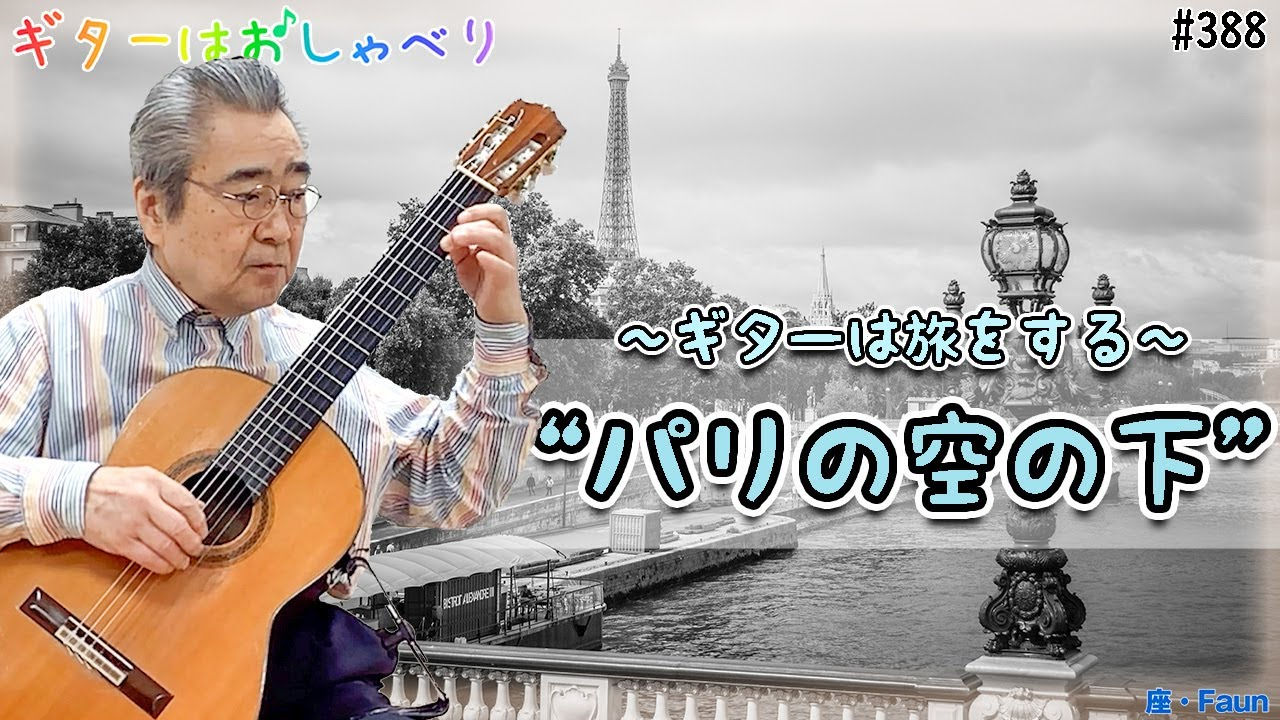
\includegraphics[width=0.48\linewidth]{pictures/youtube/2026/02/20260224_231124_youtube_001_OErGrh18mCg.jpg}
}
\end{center}




歌（シャンソン）はフランス語で聞きたいものです（ハモニカもパリっぽいですし）

\url{https://youtu.be/Vol9dZ-t93s}

\begin{center}
\href{https://youtu.be/Vol9dZ-t93s}{
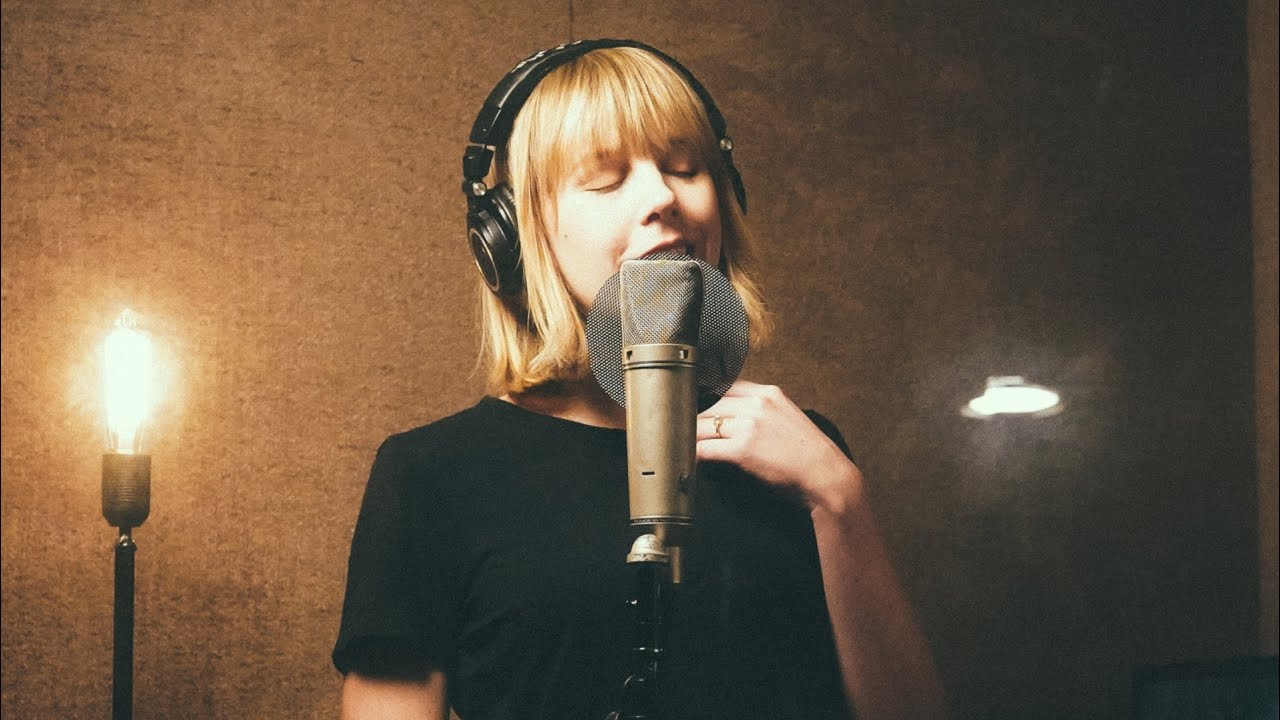
\includegraphics[width=0.48\linewidth]{pictures/youtube/2026/02/20260224_231124_youtube_002_Vol9dZ-t93s.jpg}
}
\end{center}



歌詞なんて何も分からないのに聞いていて心地良いと感じるのは何故なのか？

\subsection*{2026年02月24日 23:23}
\addcontentsline{toc}{subsection}{2026年02月24日 23:23}

\paragraph{リンク}
\url{https://youtu.be/oW2QZ7KuaxA}

\begin{center}
\href{https://youtu.be/oW2QZ7KuaxA}{

\includegraphics[width=0.48\linewidth]{pictures/youtube/2026/02/20260224_232316_youtube_001_oW2QZ7KuaxA.jpg}
}
\end{center}

\subsection*{2026年02月25日 19:33}
\addcontentsline{toc}{subsection}{2026年02月25日 19:33}

\paragraph{リンク}
\url{https://youtu.be/ZhqA3dRwWUM}

\begin{center}
\href{https://youtu.be/ZhqA3dRwWUM}{
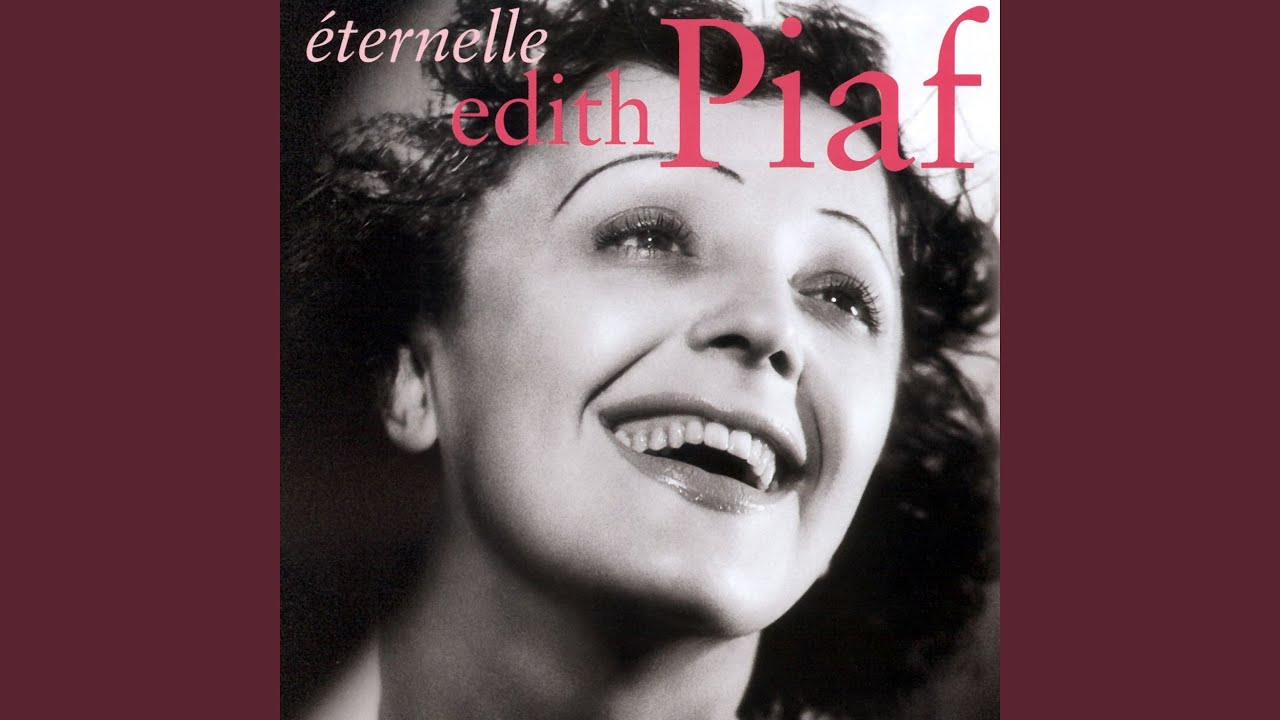
\includegraphics[width=0.48\linewidth]{pictures/youtube/2026/02/20260225_193311_youtube_001_ZhqA3dRwWUM.jpg}
}
\end{center}

\subsection*{2026年02月25日 19:35}
\addcontentsline{toc}{subsection}{2026年02月25日 19:35}

\paragraph{リンク}
\url{https://youtu.be/z1pVHaNALoI}

\begin{center}
\href{https://youtu.be/z1pVHaNALoI}{
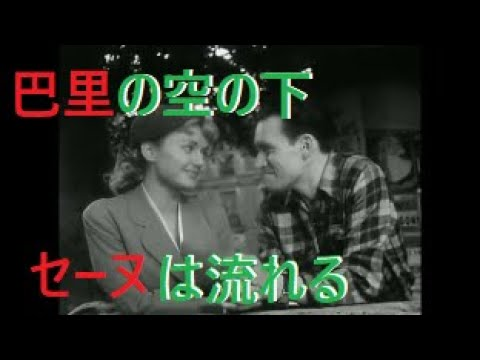
\includegraphics[width=0.48\linewidth]{pictures/youtube/2026/02/20260225_193524_youtube_001_z1pVHaNALoI.jpg}
}
\end{center}

\subsection*{2026年02月26日 09:27}
\addcontentsline{toc}{subsection}{2026年02月26日 09:27}

\paragraph{リンク}
\url{https://www.gendaiguitar.com/products/4549767163635}

\subsection*{2026年02月26日 17:59}
\addcontentsline{toc}{subsection}{2026年02月26日 17:59}

（受験生の皆さんには大変でしたでしょうけど）

面白い写真だ


\url{https://x.com/kanazawauniv_o/status/2026899670233133557?s=61&t=5VtsOkpki6juEjPXsBq8hg}



\paragraph{写真}
\begin{center}
\begin{minipage}{0.48\linewidth}
\centering
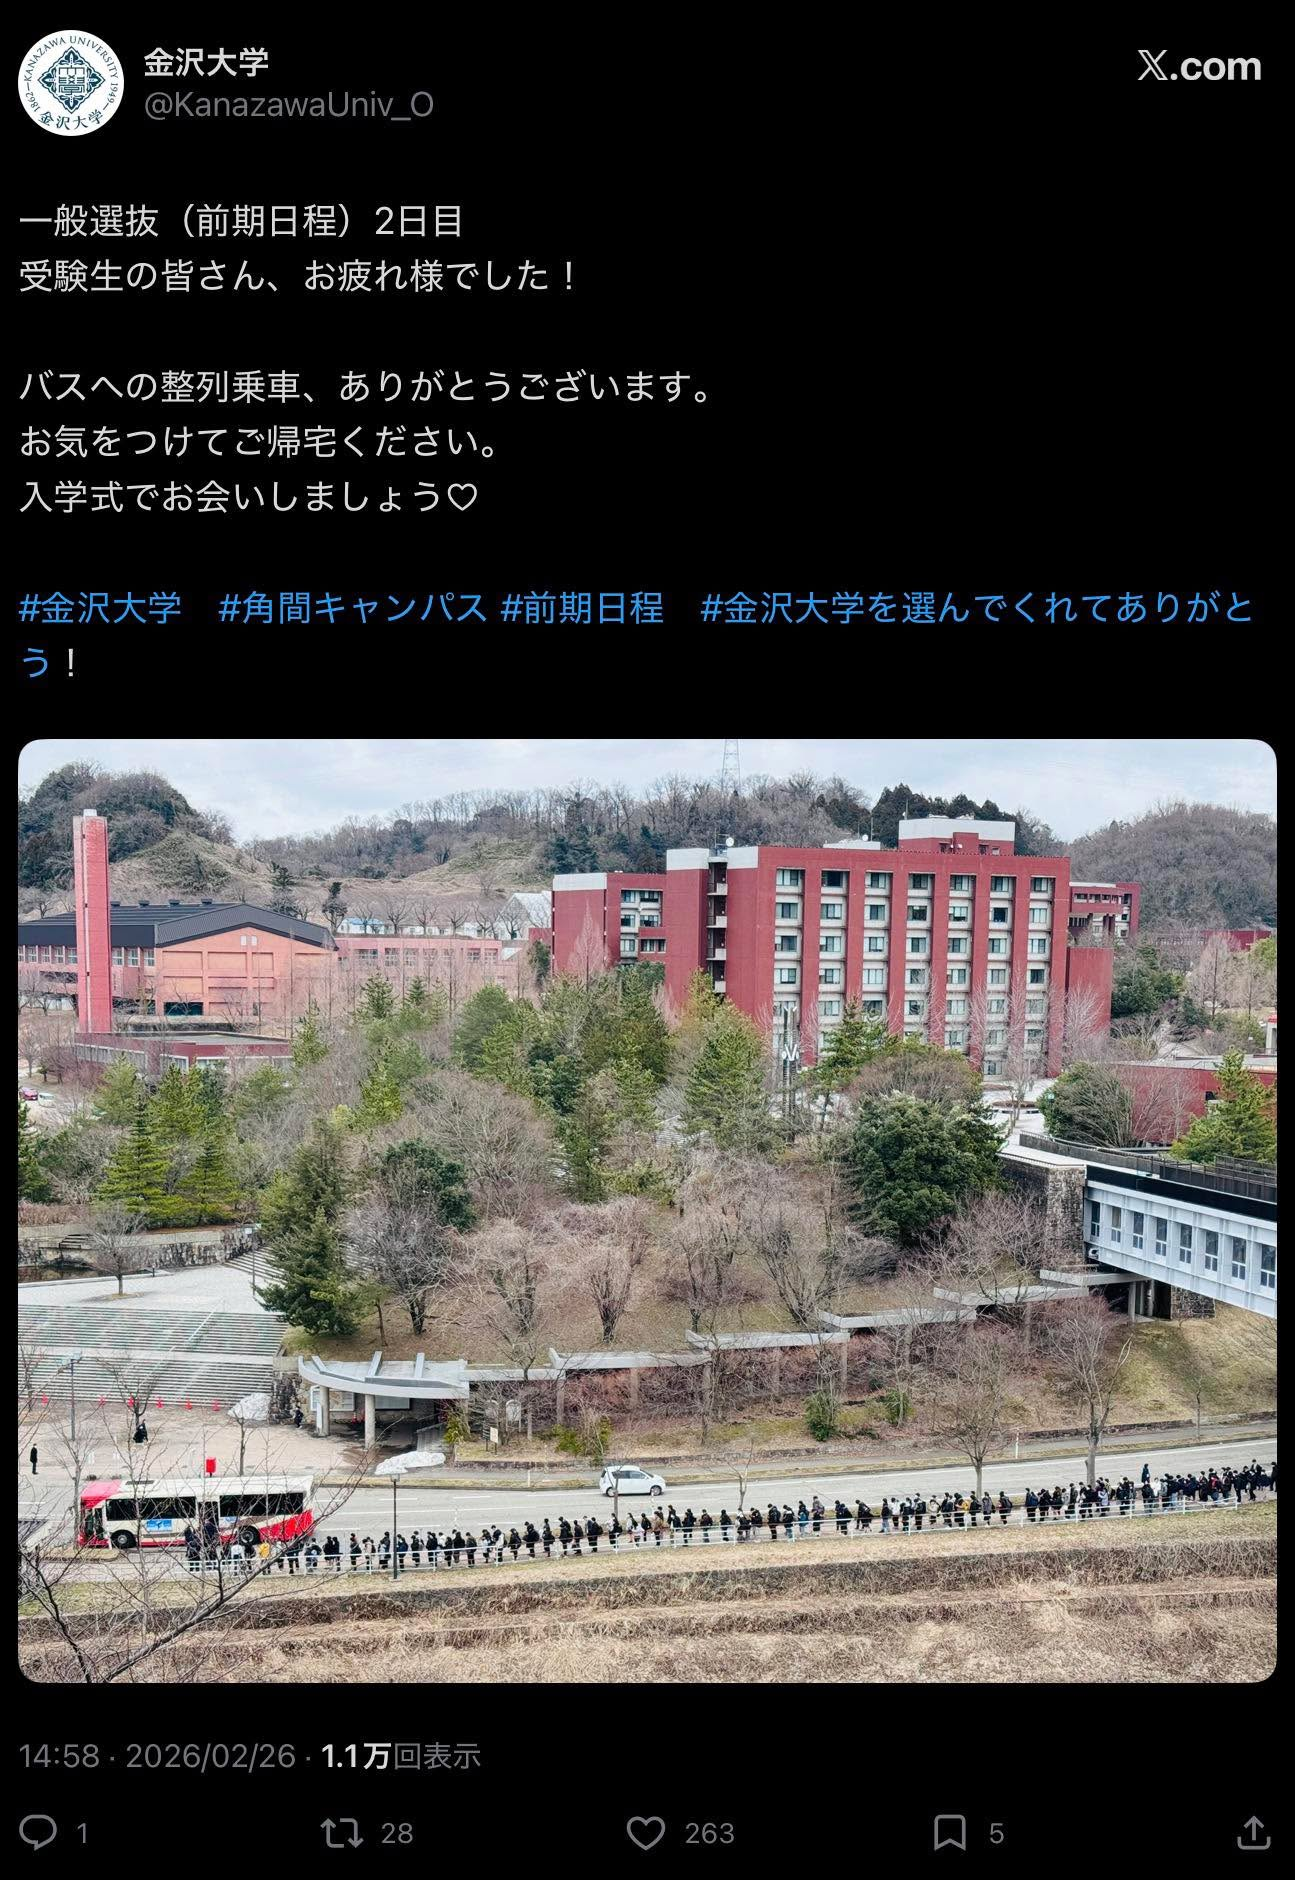
\includegraphics[width=\linewidth]{pictures/2026/02/20260226_175932_001.jpg}
\end{minipage}
\hfill
\begin{minipage}{0.48\linewidth}
\centering
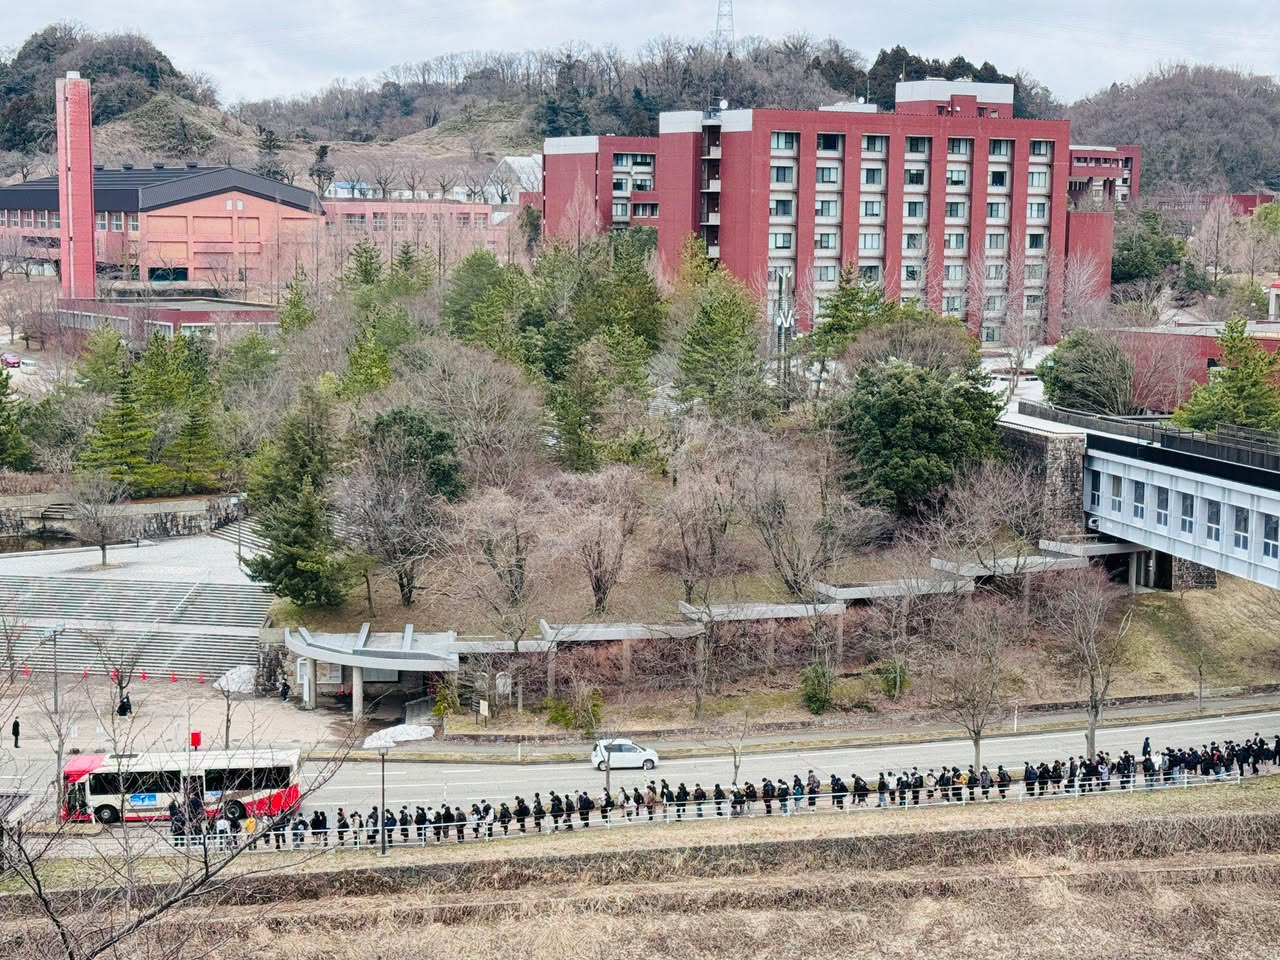
\includegraphics[width=\linewidth]{pictures/2026/02/20260226_175932_002.jpg}
\end{minipage}
\end{center}

\subsection*{2026年02月28日 10:06}
\addcontentsline{toc}{subsection}{2026年02月28日 10:06}

Fugue（BWV 998）


数ある演奏の中でも、この方（益田正洋氏）の演奏は特に、themeやphrase 、voiceなど、はっきりと聞かせてくれている様に思います

\url{https://youtu.be/80n4D_QOzUk?t=204}

\begin{center}
\href{https://youtu.be/80n4D_QOzUk?t=204}{
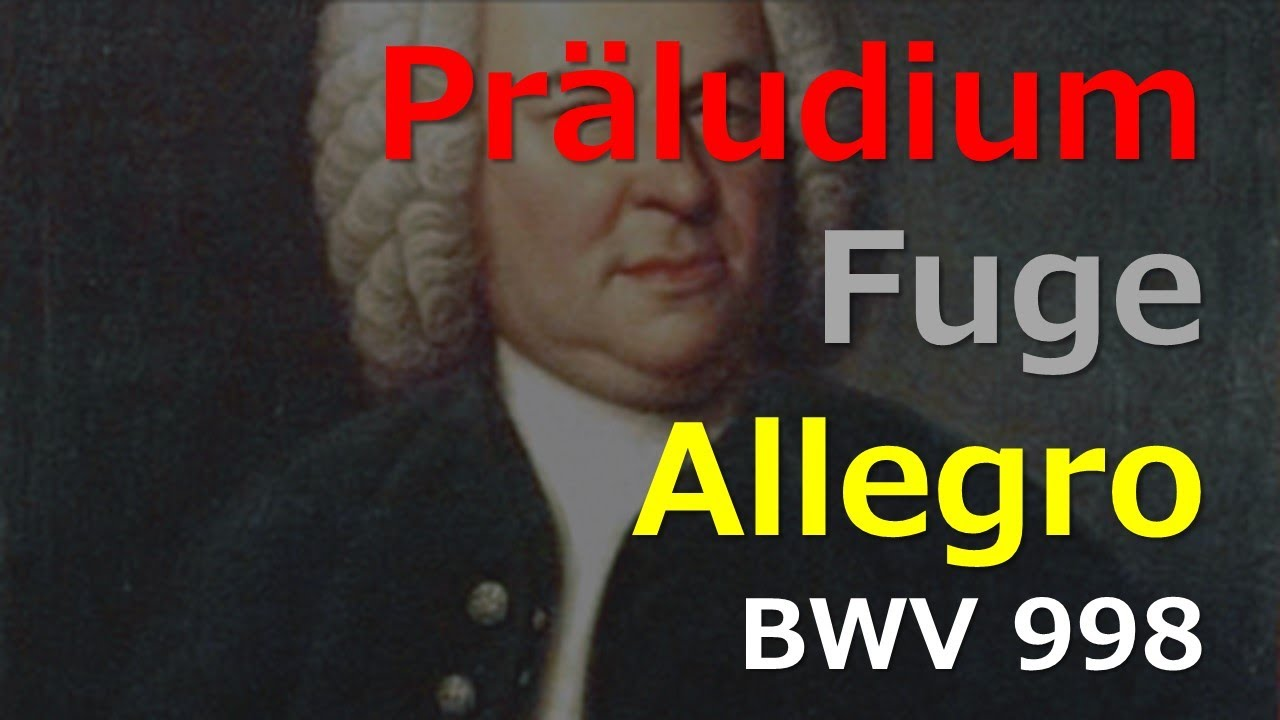
\includegraphics[width=0.48\linewidth]{pictures/youtube/2026/02/20260228_100659_youtube_001_80n4D_QOzUk.jpg}
}
\end{center}




自分で弾けていない間は（今でもなかなか弾けていないんだけど）、何となく主題が（或いはその断片が）あちらこちらに散らばっているっぽいゾ、としか思っていませんでした。でも、この方の演奏を聞いて、どこに何があるのか、どこをどの様に（フレーズとして）区切って演奏すればいいのか、などなどを（自分なりに納得しながら）決めていく様にしてみています。その事によって少しずつですが、全体的な構造が俯瞰的に見えるような気がしています。


===

この記事は以下↓の記事の続きです

\url{https://m.facebook.com/story.php?story_fbid=25765009936489824&id=100002225117991}



\subsection*{2026年02月28日 10:08}
\addcontentsline{toc}{subsection}{2026年02月28日 10:08}

\paragraph{リンク}
\url{https://youtu.be/UGQFnJDCRls}

\begin{center}
\href{https://youtu.be/UGQFnJDCRls}{
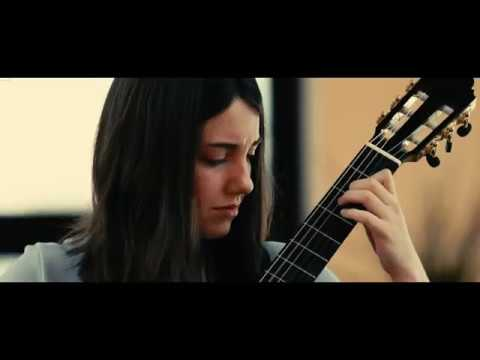
\includegraphics[width=0.48\linewidth]{pictures/youtube/2026/02/20260228_100827_youtube_001_UGQFnJDCRls.jpg}
}
\end{center}

\section{3月}

\subsection*{2026年03月01日 04:40}
\addcontentsline{toc}{subsection}{2026年03月01日 04:40}

Another Axis of Evil !

US （トランプ）🇺🇸-イスラエル（ネタニエフ）🇮🇱 -ロシア（プーチン）🇷🇺

（日本🇯🇵が、何れかのAxesの片棒を担ぐなどという事、ありません様に）


\url{https://m.facebook.com/story.php?story_fbid=3561215607351079&id=100003880233043}




===

以下の記事の続きです

\url{https://m.facebook.com/story.php?story_fbid=25462775950046559&id=100002225117991}



\subsection*{2026年03月02日 02:12}
\addcontentsline{toc}{subsection}{2026年03月02日 02:12}

パッヘルベルのカノン

色々なギター演奏テクニックを駆使して聞かせてくれているのはユニーク

面白い

\url{https://youtu.be/sE_sevj6wtg}

\begin{center}
\href{https://youtu.be/sE_sevj6wtg}{
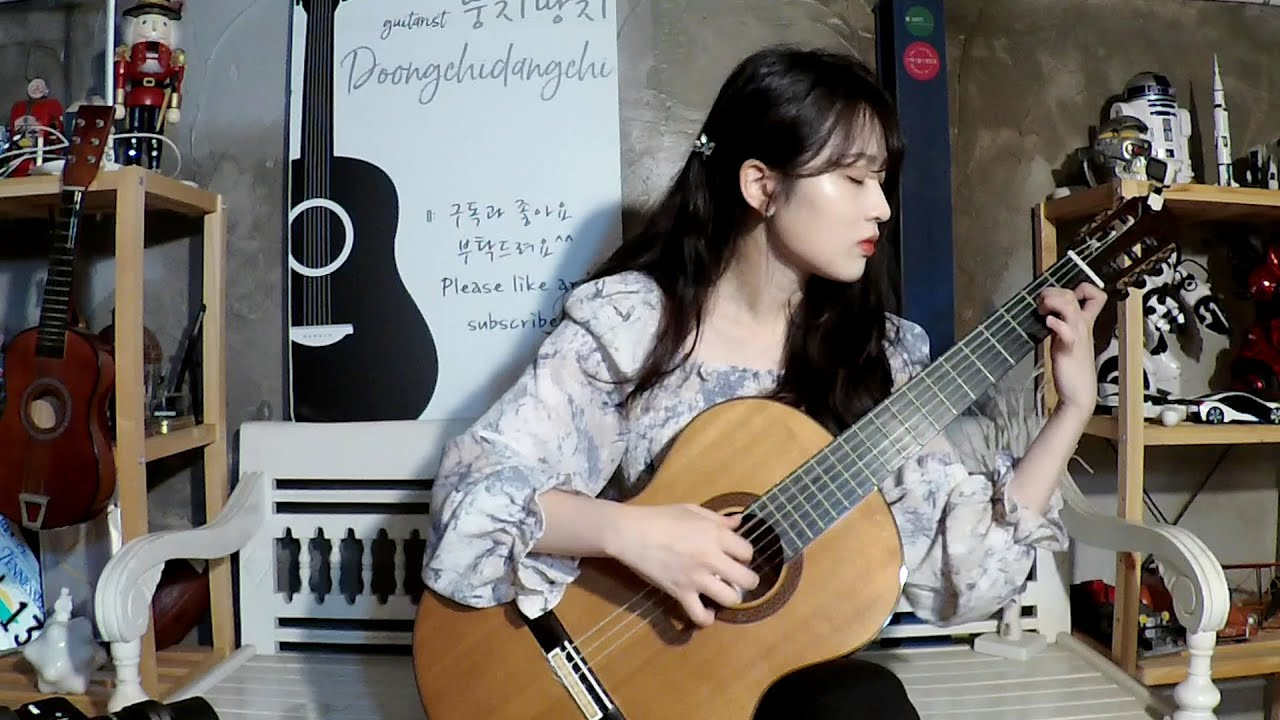
\includegraphics[width=0.48\linewidth]{pictures/youtube/2026/03/20260302_021203_youtube_001_sE_sevj6wtg.jpg}
}
\end{center}



楽譜にハーモニクスが出てくると、それだけで苦手意識に襲われる（←私の場合）と言うのに、この方はハーモニクス自由自在ですね

\subsection*{2026年03月02日 02:33}
\addcontentsline{toc}{subsection}{2026年03月02日 02:33}

\paragraph{リンク}
\url{https://youtu.be/YWGJXL1EIkw}

\begin{center}
\href{https://youtu.be/YWGJXL1EIkw}{
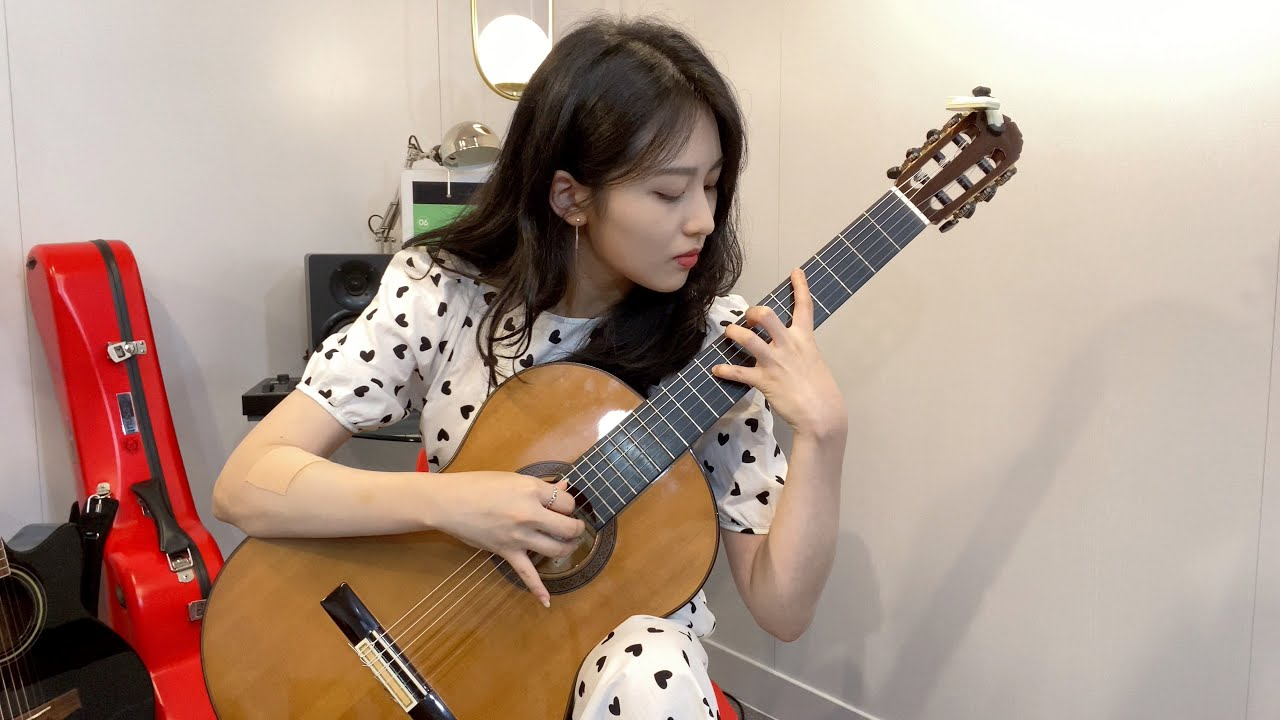
\includegraphics[width=0.48\linewidth]{pictures/youtube/2026/03/20260302_023310_youtube_001_YWGJXL1EIkw.jpg}
}
\end{center}

\subsection*{2026年03月02日 09:23}
\addcontentsline{toc}{subsection}{2026年03月02日 09:23}

\paragraph{リンク}
\url{https://youtu.be/PToaMND2L8E}

\begin{center}
\href{https://youtu.be/PToaMND2L8E}{
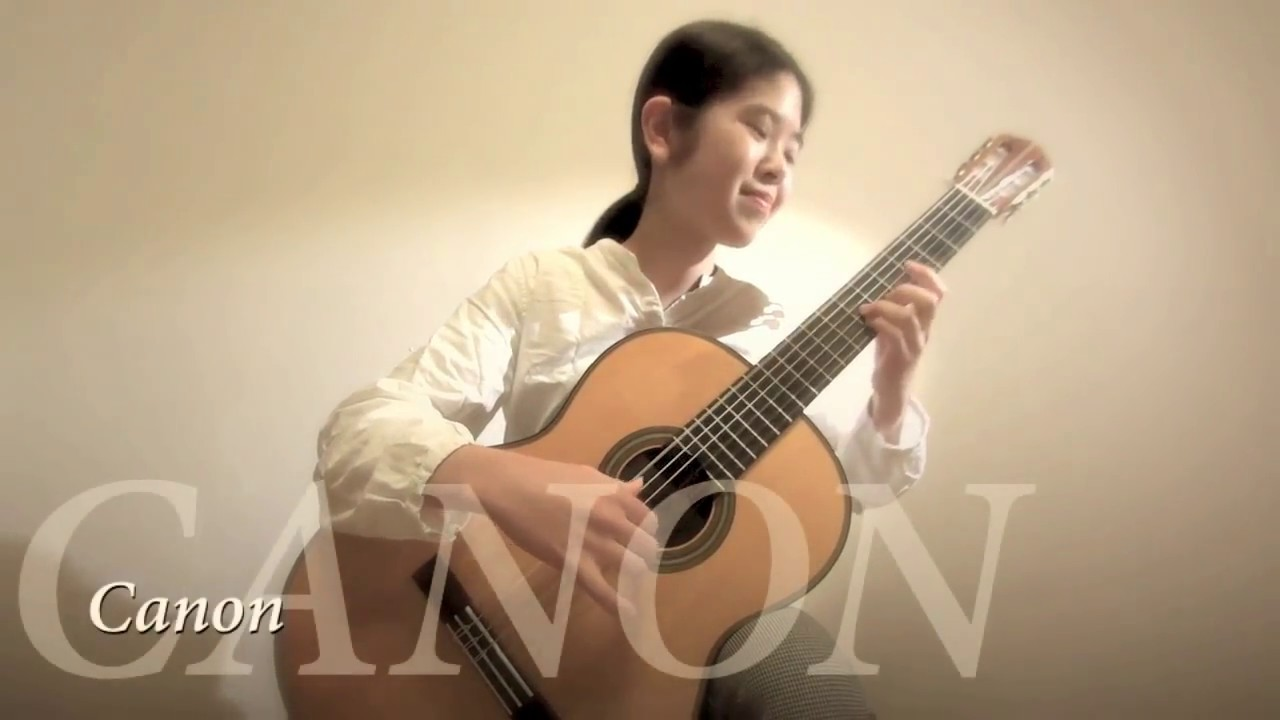
\includegraphics[width=0.48\linewidth]{pictures/youtube/2026/03/20260302_092308_youtube_001_PToaMND2L8E.jpg}
}
\end{center}

\subsection*{2026年03月04日 10:37}
\addcontentsline{toc}{subsection}{2026年03月04日 10:37}

「クラシック・ギターを極めるには一生と半分かかる」（ジュリアン・ブリーム）一生では極めきれないという意味でしょうか？


\url{https://m.facebook.com/groups/5430518938/permalink/10165044823833939/}




これには、

「クラシック・ギターをマスターするには一生半かかる（未だ道半ばだ）」

括弧内の含意がある（むしろ括弧内と同義なのでは？）

It takes a lifetime and a half to master the classical guitar, yet I'm still halfway there.（DeepL翻訳）


ブリームの様な名手にして道半ばとの認識でいらしたという事か

「自分なりに追求していきたい」と思わせてくれる（やる気の出る）写真です

ギターを抱えて演奏している表情がとても良い←何ていう曲のどの部分かは分からないけど、何となく気持ちが分かる様な気がします

\paragraph{写真}
\begin{center}
\begin{minipage}{0.48\linewidth}
\centering
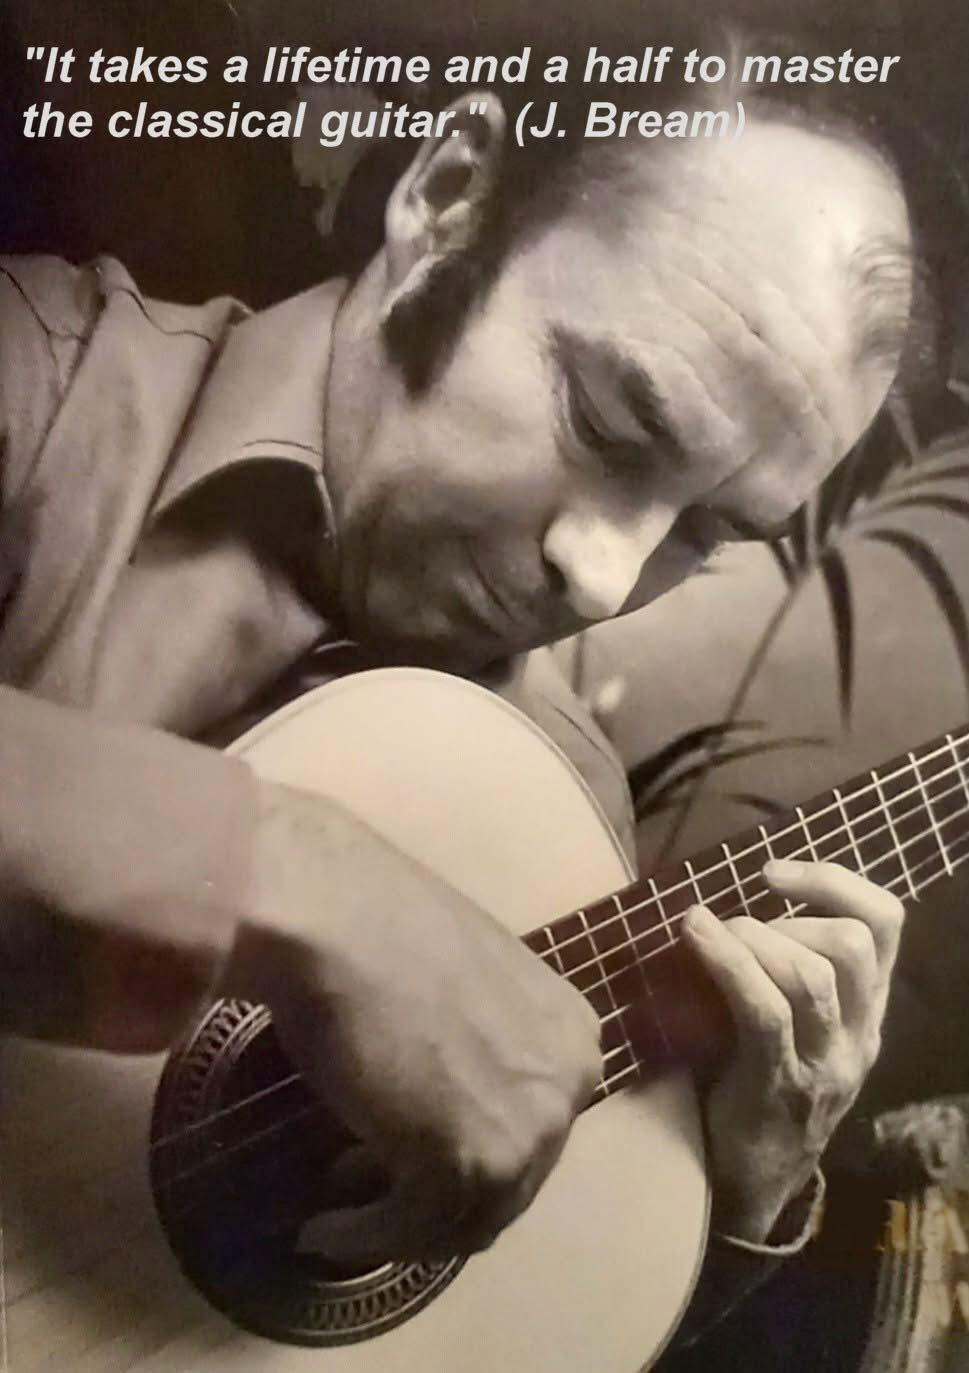
\includegraphics[width=\linewidth]{pictures/2026/03/20260304_103717_001.jpg}
\end{minipage}
\end{center}

\subsection*{2026年03月05日 21:03}
\addcontentsline{toc}{subsection}{2026年03月05日 21:03}

\paragraph{リンク}
\url{https://youtu.be/0J-MtvrfcrA}

\begin{center}
\href{https://youtu.be/0J-MtvrfcrA}{
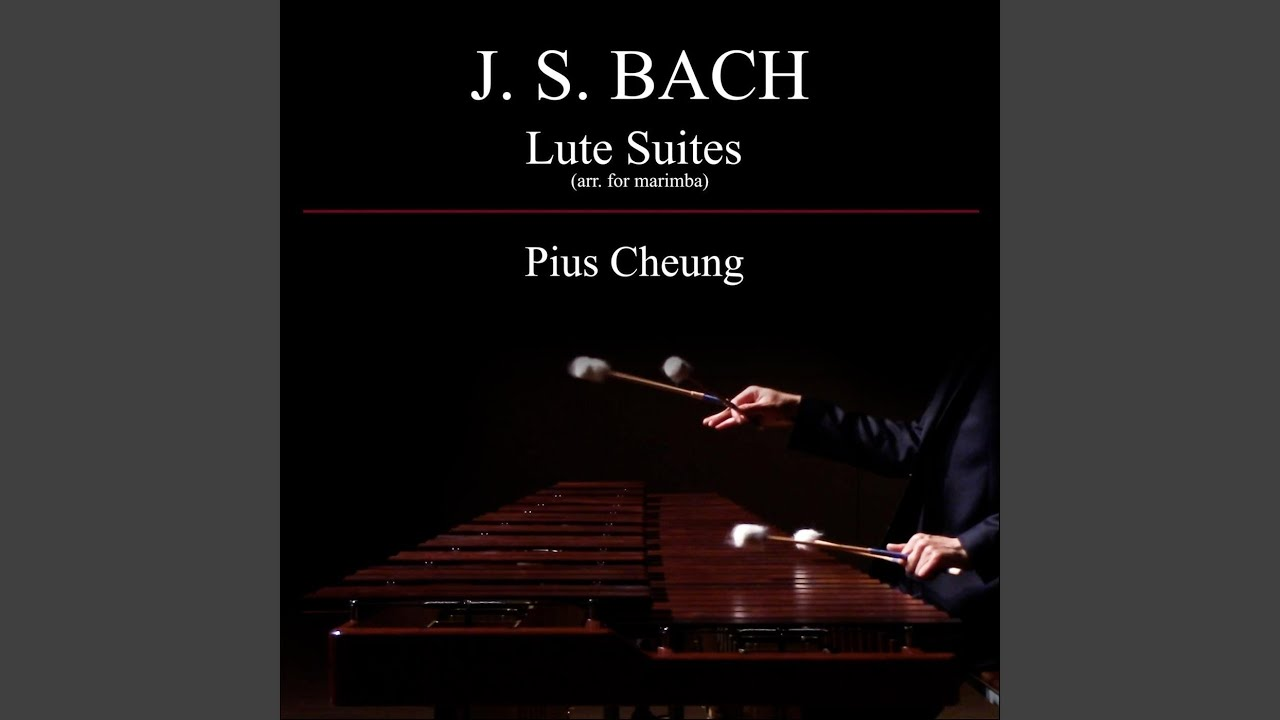
\includegraphics[width=0.48\linewidth]{pictures/youtube/2026/03/20260305_210334_youtube_001_0J-MtvrfcrA.jpg}
}
\end{center}

\subsection*{2026年03月05日 22:01}
\addcontentsline{toc}{subsection}{2026年03月05日 22:01}

\paragraph{リンク}
\url{https://youtu.be/GOA3R3h9AW0}

\begin{center}
\href{https://youtu.be/GOA3R3h9AW0}{
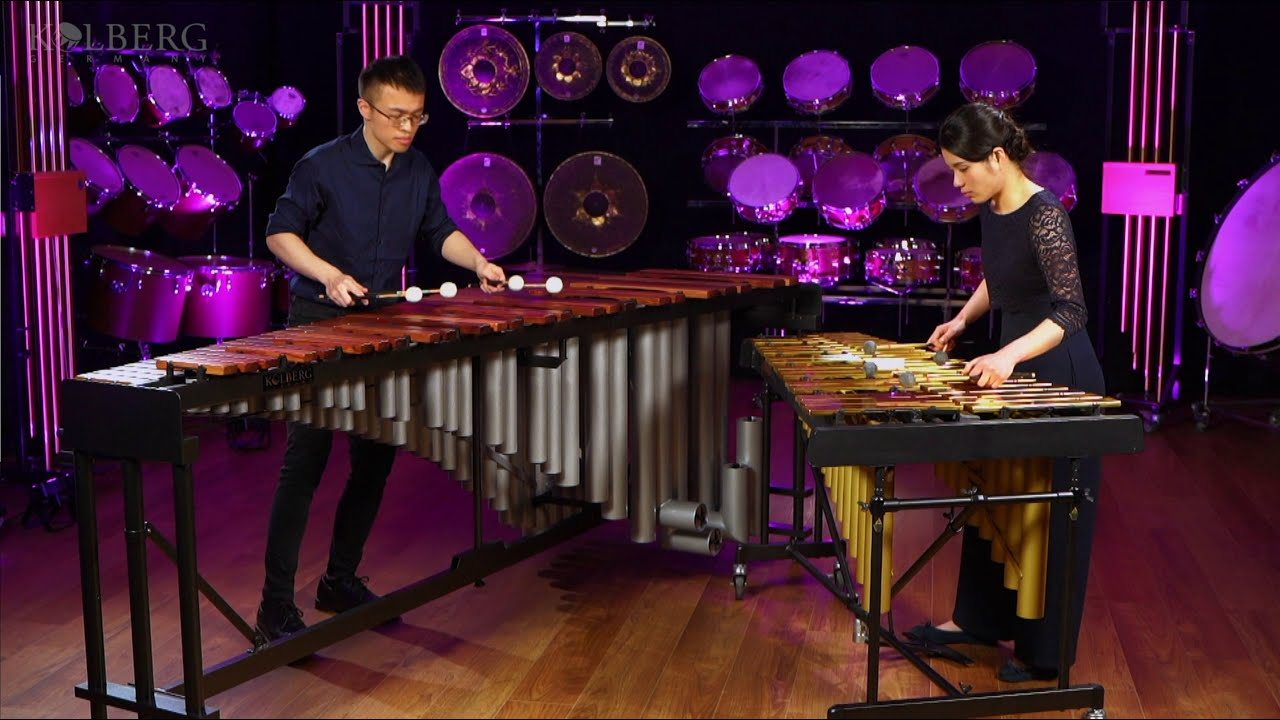
\includegraphics[width=0.48\linewidth]{pictures/youtube/2026/03/20260305_220154_youtube_001_GOA3R3h9AW0.jpg}
}
\end{center}

\subsection*{2026年03月06日 08:47}
\addcontentsline{toc}{subsection}{2026年03月06日 08:47}

これは公開しない


国防長官もその通りだが、副大統領もひどい！ゼレンスキー大統領を怒鳴りつけていた時から困った連中だと思っていた。大統領も含めて、短絡的で単細胞な思考回路の持ち主。幼稚なチンピラと同じ。トランプが大統領になっていなかったなら、死ななくて済んだ人達、その家族が沢山いるんですから。


\url{https://www.facebook.com/100003050293182/posts/25841038545581135/}




===

以下の記事の続きです

\url{https://m.facebook.com/story.php?story_fbid=25946560035001479&id=100002225117991}



\subsection*{2026年03月07日 00:52}
\addcontentsline{toc}{subsection}{2026年03月07日 00:52}

英仏伊が西に賛同する姿勢を示しているが、日独加はイランを非難している様だ（困ったものだ）独はイスラエル＝ユダヤ人に忖度している所があるかもしれません


\url{https://www.facebook.com/100079265598948/posts/906968011955377/}




元々はスペイン政府が公にしている英訳記事。この朝日新聞の記事は残念ながら有料！（なので読めない）


サンチェス首相（Pedro Sánchez）が 2026年3月4日にテレビで行った声明。その英語版（スペイン政府による翻訳）は、次の公式PDFで読める


\url{https://www.lamoncloa.gob.es/presidente/intervenciones/Documents/2026/260304-INSTITUTIONAL-STATEMENT-BY-THE-SPANISH-PRIME-MINISTER-PEDRO\%20SA\%CC\%81NCHEZ-CONCERNING-THE-RECENT-INTERNATIONAL-EVENTS.pdf}




DeepLやChatGPTなどに日本語にしてと頼めば、有料記事に頼らなくてもOk


戦争反対！（このごく単純な言葉=思いを、いつでも誰に臆するでもなく発することができる、その様な日本であり続けて欲しい）


===

以下の記事の続きです

\url{https://m.facebook.com/story.php?story_fbid=25946560035001479&id=100002225117991}



\paragraph{リンク}
\url{https://www.asahi.com/articles/ASV354QQDV35UHBI030M.html?ref=facebook}

\subsection*{2026年03月07日 23:45}
\addcontentsline{toc}{subsection}{2026年03月07日 23:45}

\paragraph{リンク}
\url{https://youtu.be/DQCwG70mohc}

\begin{center}
\href{https://youtu.be/DQCwG70mohc}{
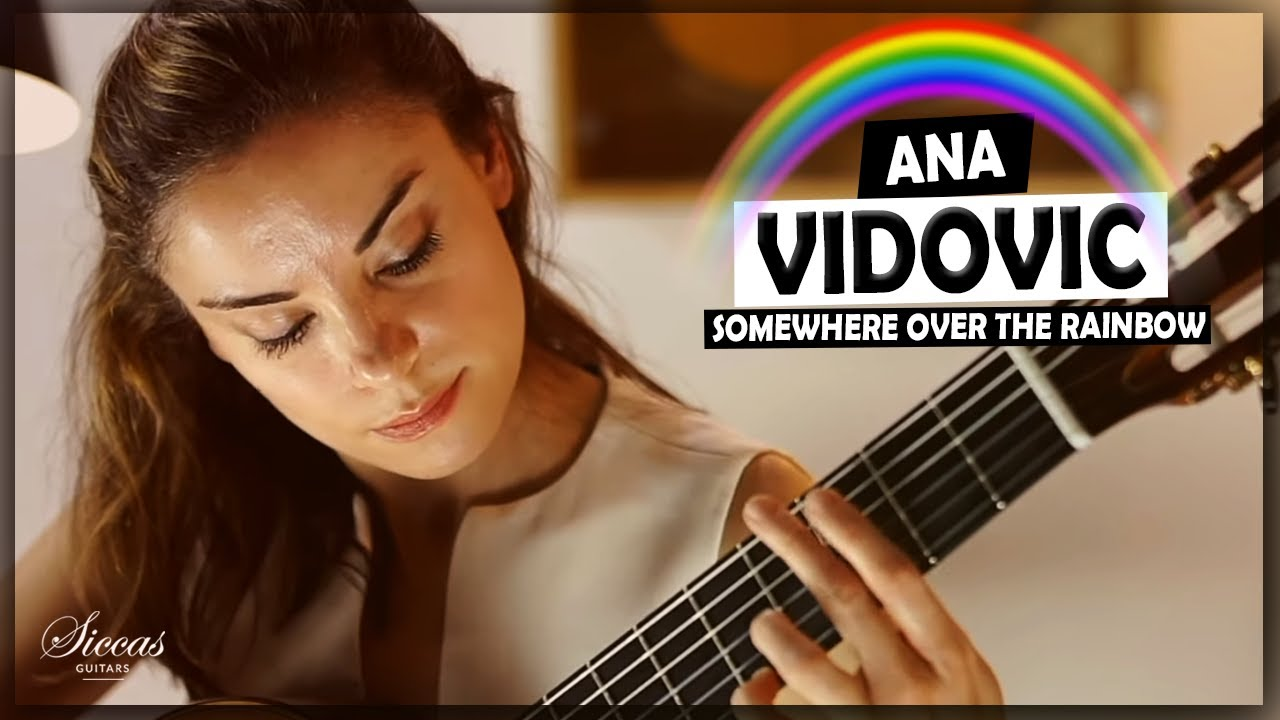
\includegraphics[width=0.48\linewidth]{pictures/youtube/2026/03/20260307_234506_youtube_001_DQCwG70mohc.jpg}
}
\end{center}

\subsection*{2026年03月07日 23:47}
\addcontentsline{toc}{subsection}{2026年03月07日 23:47}

\paragraph{リンク}
\url{https://youtu.be/inc7THXyJ1o}

\begin{center}
\href{https://youtu.be/inc7THXyJ1o}{
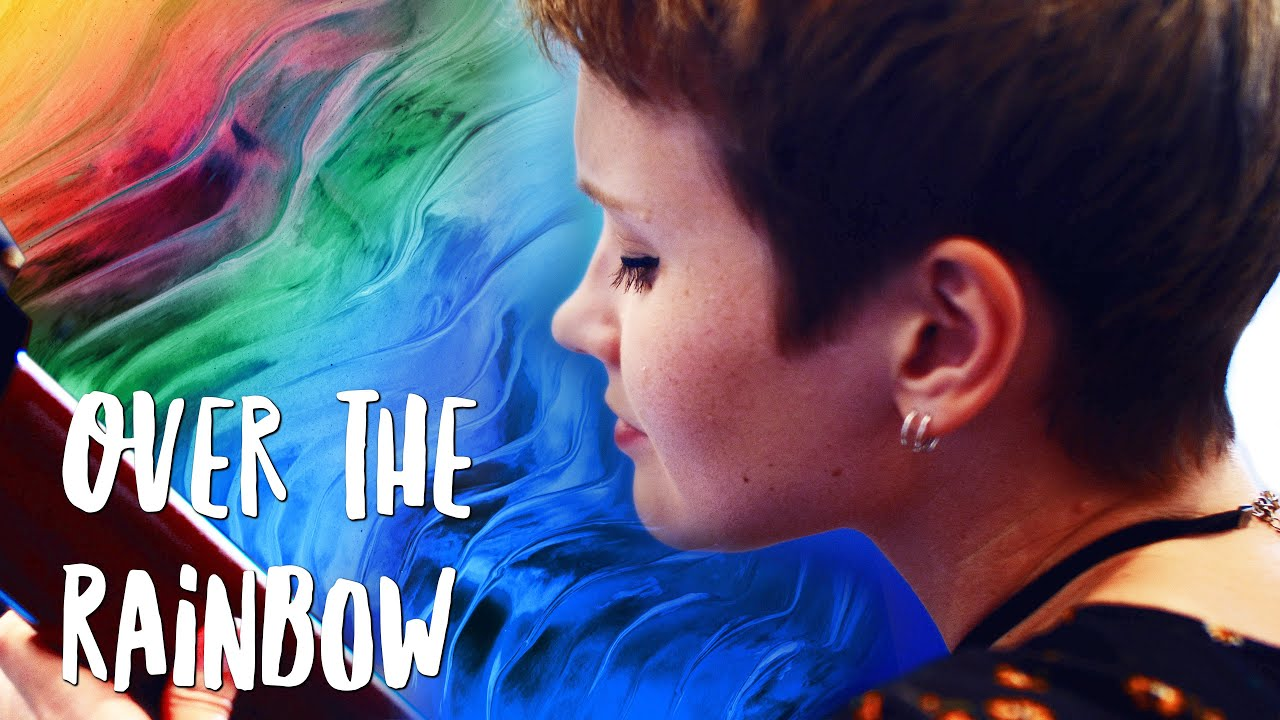
\includegraphics[width=0.48\linewidth]{pictures/youtube/2026/03/20260307_234737_youtube_001_inc7THXyJ1o.jpg}
}
\end{center}

\subsection*{2026年03月08日 00:02}
\addcontentsline{toc}{subsection}{2026年03月08日 00:02}

\paragraph{リンク}
\url{https://youtu.be/QENJrG8YrGc}

\begin{center}
\href{https://youtu.be/QENJrG8YrGc}{
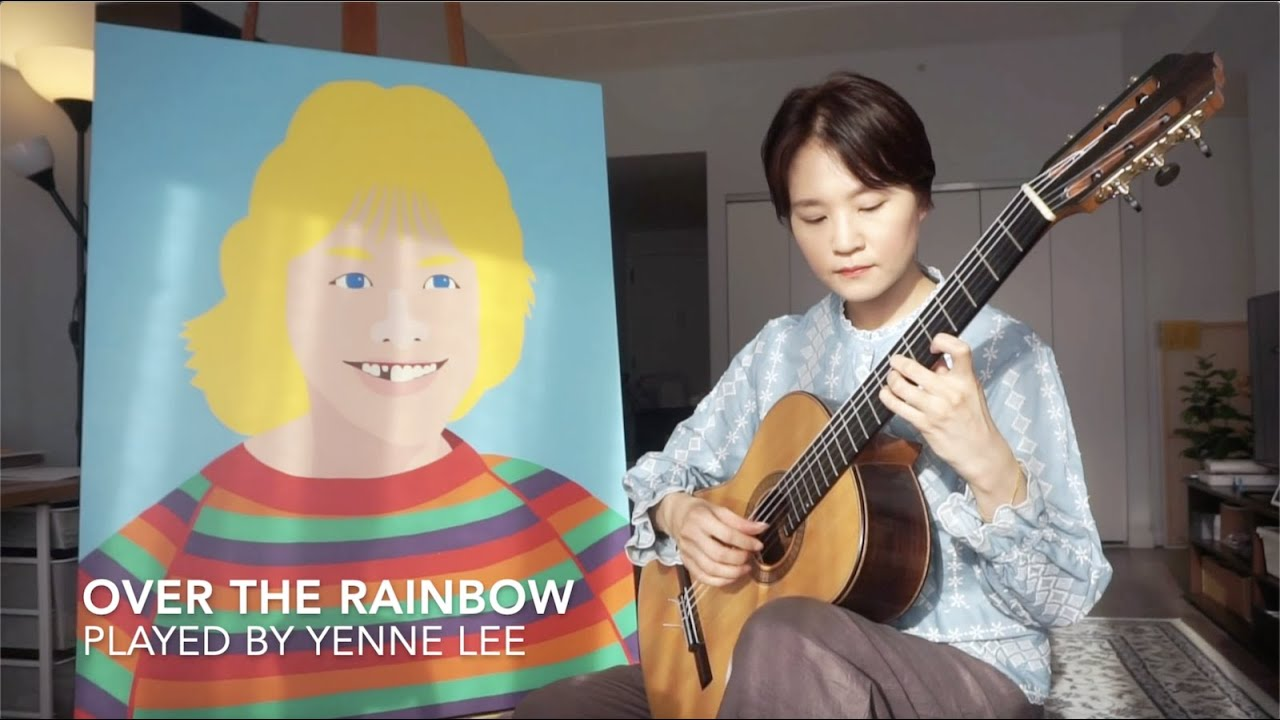
\includegraphics[width=0.48\linewidth]{pictures/youtube/2026/03/20260308_000255_youtube_001_QENJrG8YrGc.jpg}
}
\end{center}

\subsection*{2026年03月08日 00:54}
\addcontentsline{toc}{subsection}{2026年03月08日 00:54}

\paragraph{リンク}
\url{https://youtu.be/oW2QZ7KuaxA}

\begin{center}
\href{https://youtu.be/oW2QZ7KuaxA}{

\includegraphics[width=0.48\linewidth]{pictures/youtube/2026/03/20260308_005435_youtube_001_oW2QZ7KuaxA.jpg}
}
\end{center}

\subsection*{2026年03月08日 13:23}
\addcontentsline{toc}{subsection}{2026年03月08日 13:23}

\paragraph{リンク}
\url{https://youtu.be/eNlWjGOSm-U}

\begin{center}
\href{https://youtu.be/eNlWjGOSm-U}{
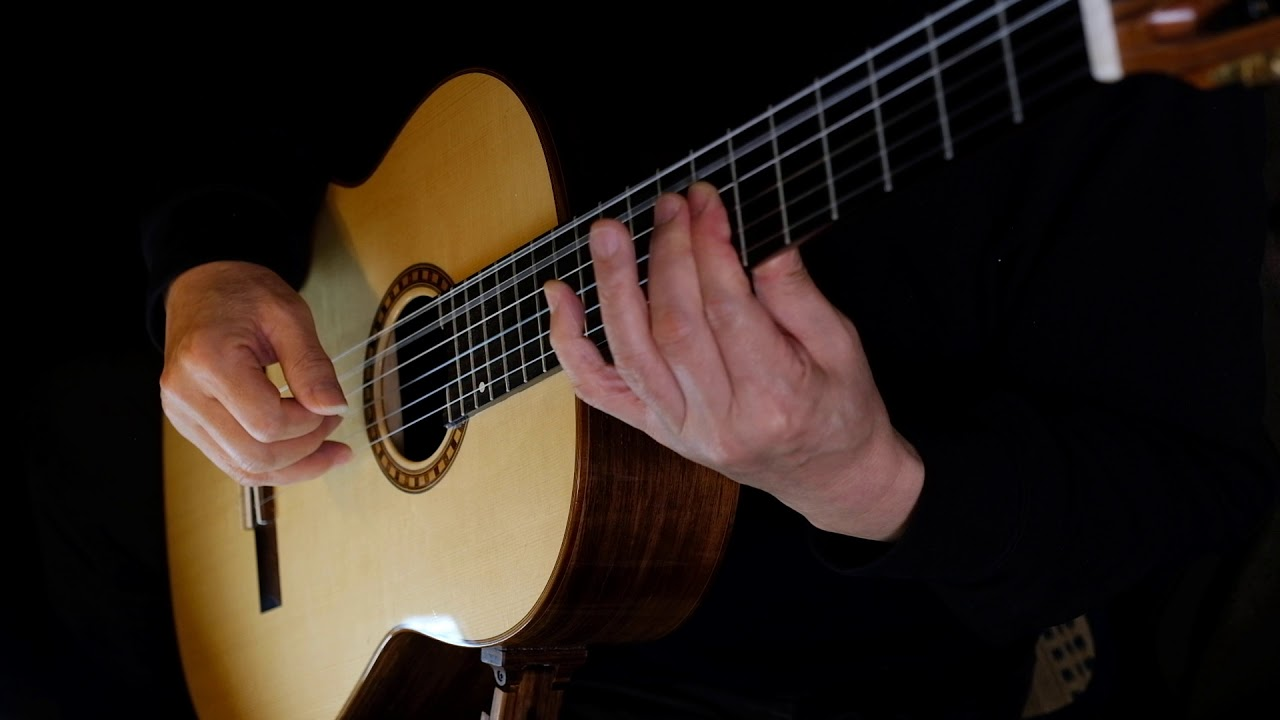
\includegraphics[width=0.48\linewidth]{pictures/youtube/2026/03/20260308_132322_youtube_001_eNlWjGOSm-U.jpg}
}
\end{center}

\subsection*{2026年03月08日 22:23}
\addcontentsline{toc}{subsection}{2026年03月08日 22:23}

\paragraph{リンク}
\url{https://youtu.be/4_tliAvZwWQ}

\begin{center}
\href{https://youtu.be/4_tliAvZwWQ}{
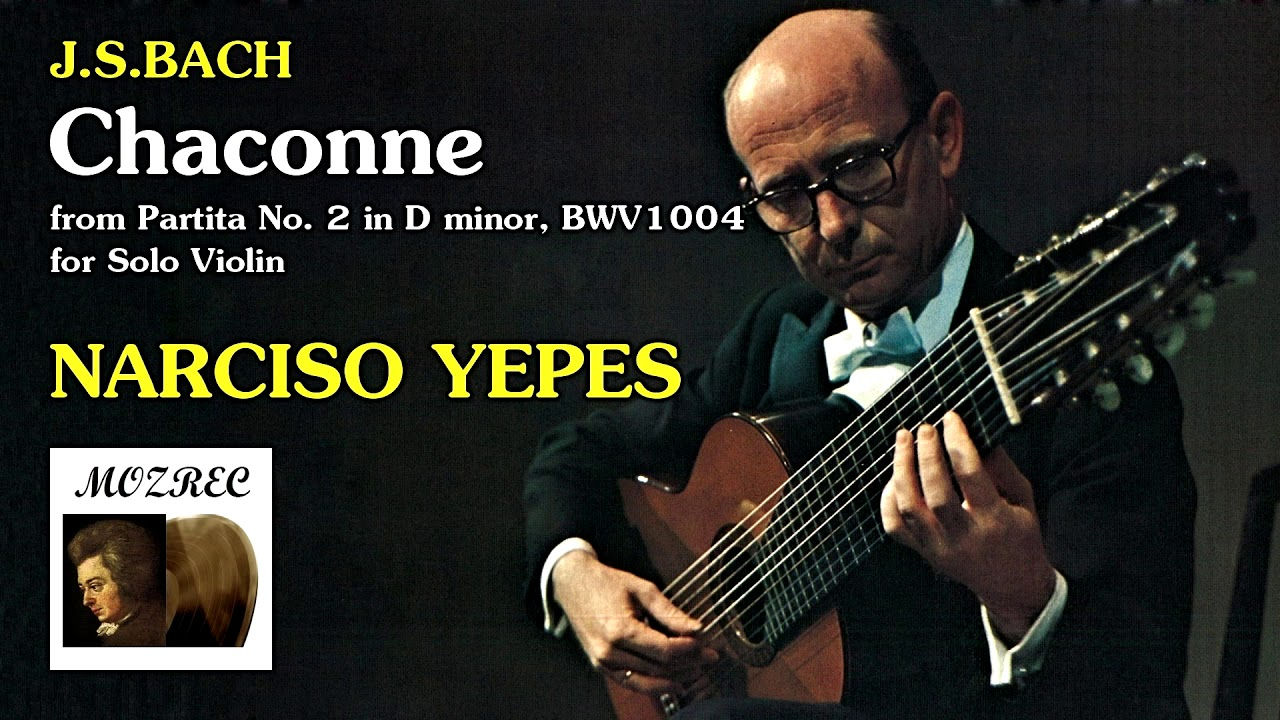
\includegraphics[width=0.48\linewidth]{pictures/youtube/2026/03/20260308_222359_youtube_001_4_tliAvZwWQ.jpg}
}
\end{center}

\subsection*{2026年03月09日 05:47}
\addcontentsline{toc}{subsection}{2026年03月09日 05:47}

\paragraph{リンク}
\url{https://youtu.be/ZLVKDfYZHVc}

\begin{center}
\href{https://youtu.be/ZLVKDfYZHVc}{
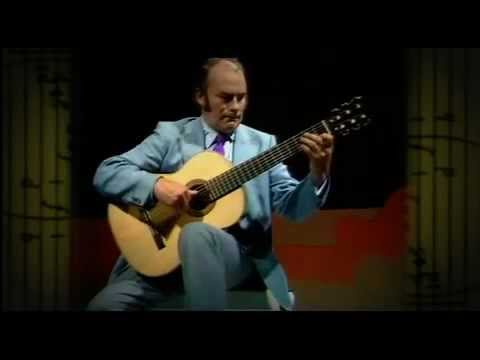
\includegraphics[width=0.48\linewidth]{pictures/youtube/2026/03/20260309_054736_youtube_001_ZLVKDfYZHVc.jpg}
}
\end{center}

\subsection*{2026年03月09日 06:14}
\addcontentsline{toc}{subsection}{2026年03月09日 06:14}

「いちばん最後」まで聞いて（見て）頂きたくなる演奏（映像）ですね

\url{https://youtu.be/nCfYe5xG1cw}

\begin{center}
\href{https://youtu.be/nCfYe5xG1cw}{
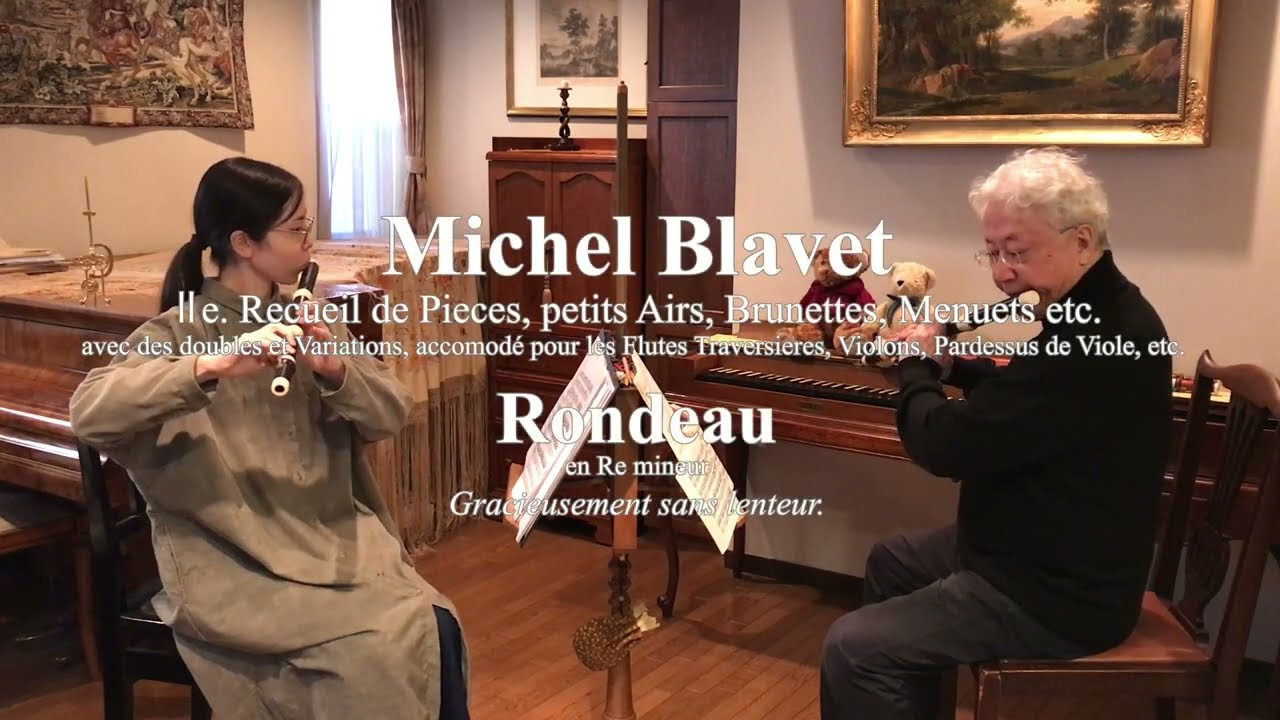
\includegraphics[width=0.48\linewidth]{pictures/youtube/2026/03/20260309_061458_youtube_001_nCfYe5xG1cw.jpg}
}
\end{center}



（宮戸さん、応援していますよ！かげながら）

演奏会のチケットはここ 

\url{https://teket.jp/16077/58893}

 です


Thomas Stanesby Jr.（1692-1754）ですが、良いですね

有田先生は二本作っていらしたのか（一本は見せて頂いた事がある）

トヤマ楽器Aulosから売られているステンズビーJrは、同じ製作者（ブランド）による別のモデル（のコピー）です（ネット上では混同している記事もある）


実は私も（かつて）この楽器のコピーを作ってみた事があります

有田正広先生がThomas Stanesby Jr.のオリジナル楽器を、Frans Brüggen氏( 

\url{https://www.facebook.com/100002225117991/posts/24491444063846424/}

 ）から譲り受けられ、その楽器を日本の杉原氏やカナダのJean-François Beaudin氏( 

\url{https://www.flutebeaudin.com}

 ）が計測され、その計測データを（私が）手に入れて製作してみたというわけです


製作当初は、完成したら有田先生に見てもらおうと思っていたのですが、「指孔のアンダーカット」に確信が持てなくて、いつになっても削っている様な始末。完成したという気がしませんでした。製作の途中には杉原さんのお宅に伺ってどう削ったものか聞きに行った事もありました。その内コロナが流行して、それ以来失礼している様な状態です（先生のお元気そうな姿を見られて嬉しく思います）


自分で作った楽器でTelemanのFantasyなどを自分一人吹いてみている分にはそれ程支障もありません（「こんなもんかな」と思っている）しかしながら、チェンバロ伴奏でとか、この演奏の様に二重奏でとなると、ちょっと不都合な事になりそうな気がします（つまり、「指孔のアンダーカット」とは即ち、殆ど「音程の調整」の事なのです）


===

以下は工房立ち上げ時の記事です

\url{https://m.facebook.com/story.php?story_fbid=24199140336410133&id=100002225117991}



\subsection*{2026年03月09日 18:03}
\addcontentsline{toc}{subsection}{2026年03月09日 18:03}

\url{https://youtu.be/vCH39NZGLw0}

\begin{center}
\href{https://youtu.be/vCH39NZGLw0}{
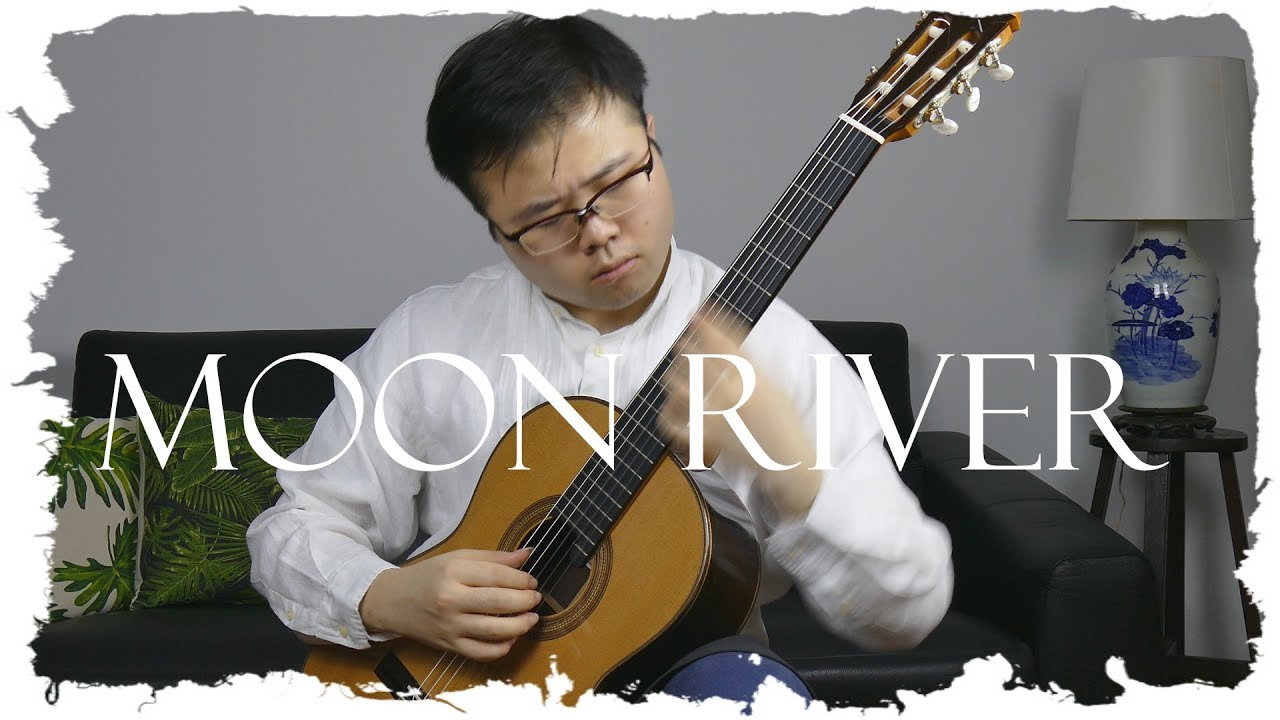
\includegraphics[width=0.48\linewidth]{pictures/youtube/2026/03/20260309_180355_youtube_001_vCH39NZGLw0.jpg}
}
\end{center}



\subsection*{2026年03月10日 00:13}
\addcontentsline{toc}{subsection}{2026年03月10日 00:13}

\paragraph{リンク}
\url{https://youtu.be/E9O1637tdtA}

\begin{center}
\href{https://youtu.be/E9O1637tdtA}{
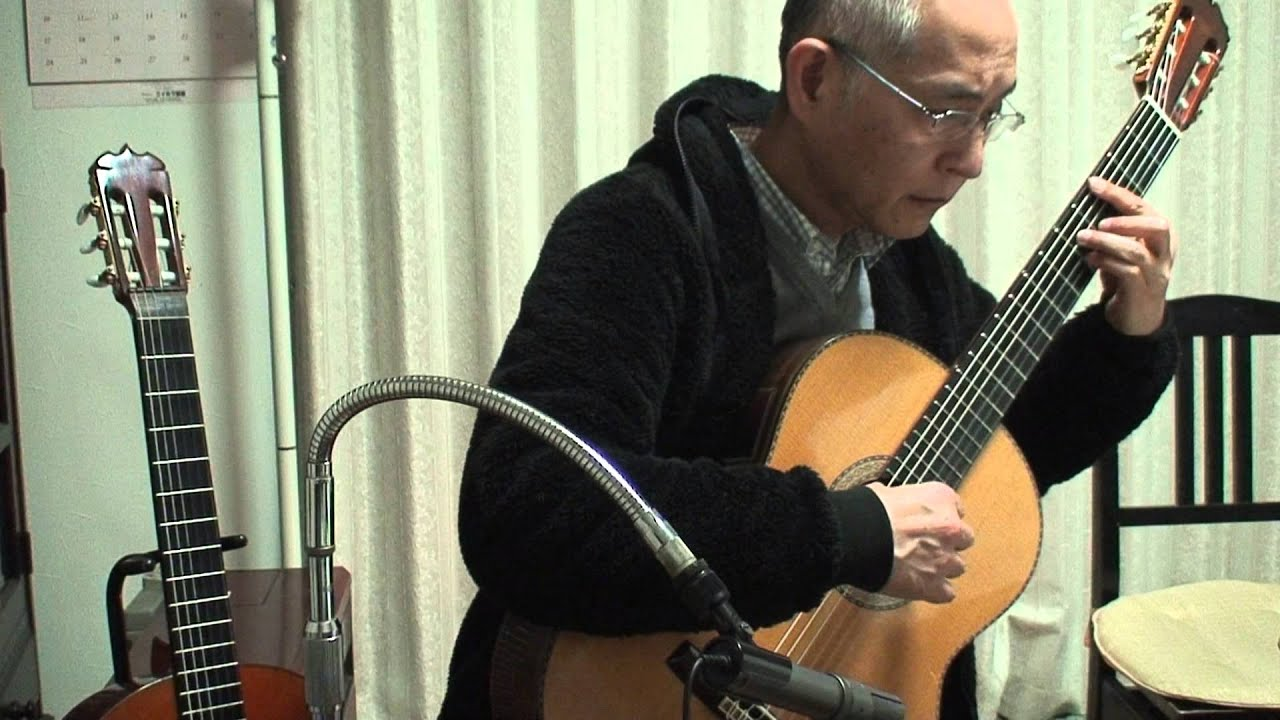
\includegraphics[width=0.48\linewidth]{pictures/youtube/2026/03/20260310_001300_youtube_001_E9O1637tdtA.jpg}
}
\end{center}

\subsection*{2026年03月11日 08:37}
\addcontentsline{toc}{subsection}{2026年03月11日 08:37}

量子コンピュータで解いてみて面白かったもの一覧（１年前はこんな事やってたのか）

プログラムやドキュメント等は全部GitHub（ 

\url{https://github.com/smat1957/QA4U}

 ）に置いています


(１)数独

\url{https://m.facebook.com/story.php?story_fbid=9619959531421455&id=100002225117991}




(２)魔方陣

\url{https://m.facebook.com/story.php?story_fbid=9573747636042645&id=100002225117991}




(３)巡回セールスマン

\url{https://m.facebook.com/story.php?story_fbid=9553924058025003&id=100002225117991}




(４)ナップザック

\url{https://m.facebook.com/story.php?story_fbid=9505203306230412&id=100002225117991}




(５)８クイーン

\url{https://m.facebook.com/story.php?story_fbid=9457796634304413&id=100002225117991}




(６)グループ分け

\url{https://m.facebook.com/story.php?story_fbid=9390581474359263&id=100002225117991}




こういう問題を考えていると、学生だった頃に月刊誌bit（共立出版）を毎月楽しみにしていた自分のこと（気持ち）を思い出します（その頃から、意味あると思っていたものって変わっていないんだと思います）

\paragraph{写真}
\begin{center}
\begin{minipage}{0.48\linewidth}
\centering
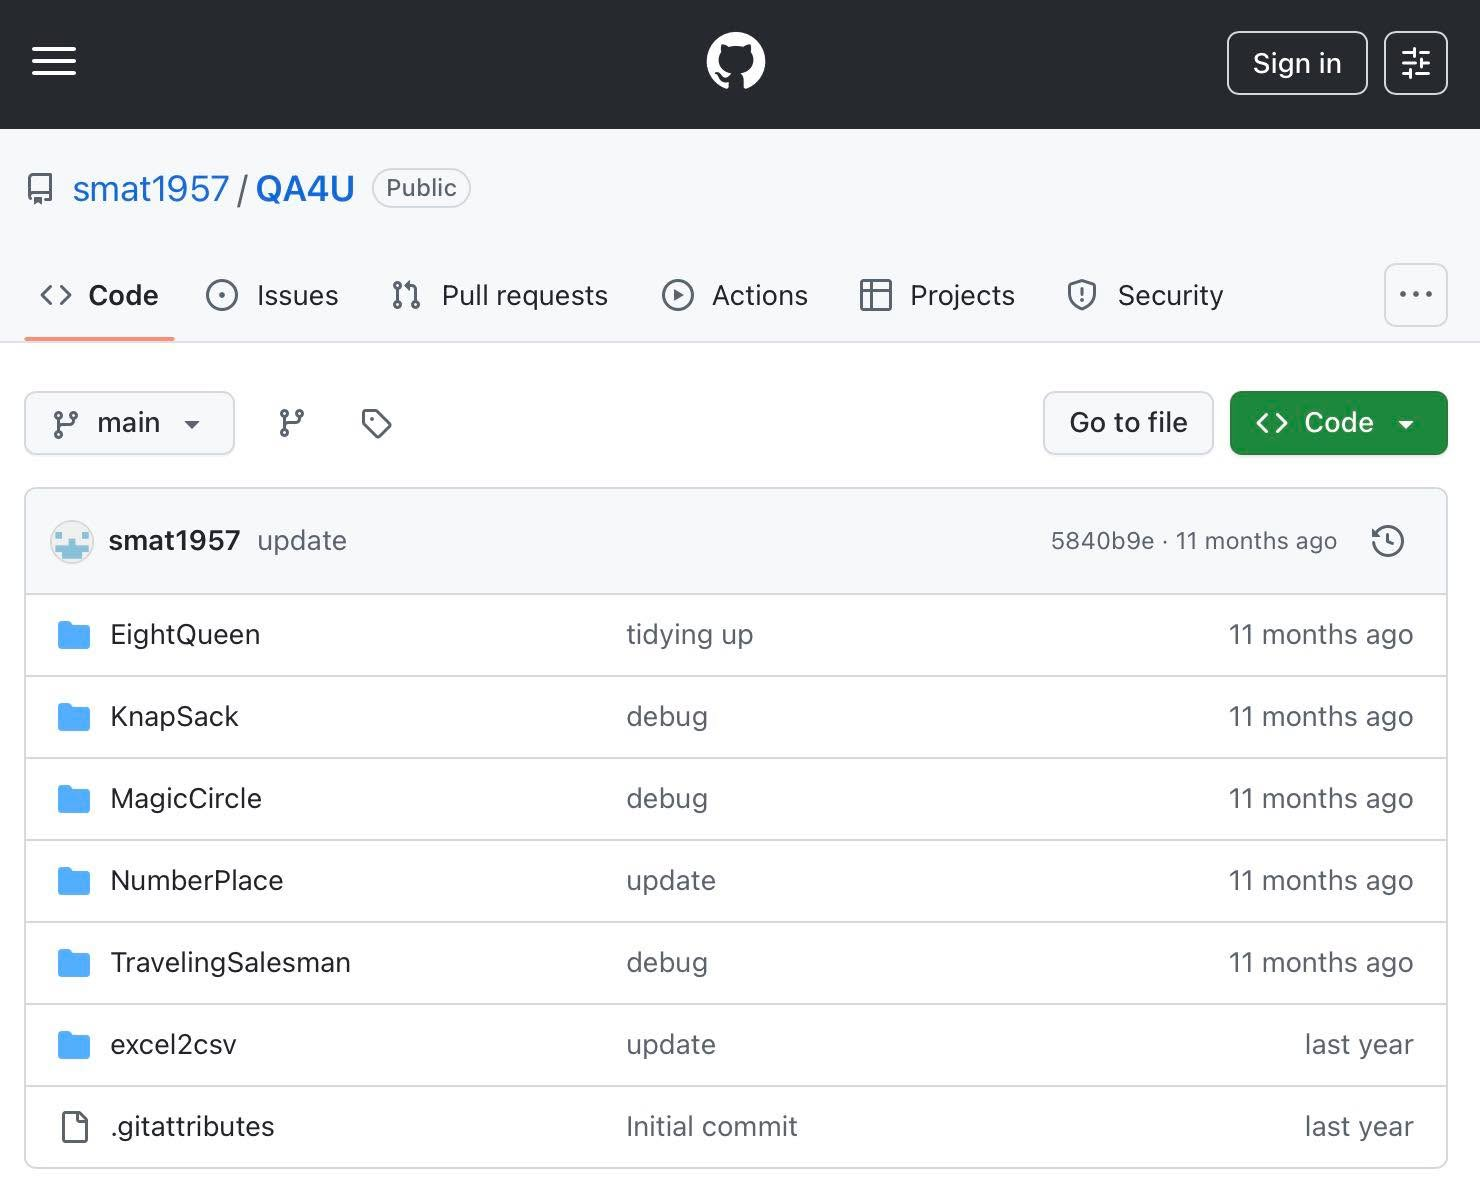
\includegraphics[width=\linewidth]{pictures/2026/03/20260311_083705_001.jpg}
\end{minipage}
\end{center}

\subsection*{2026年03月11日 20:16}
\addcontentsline{toc}{subsection}{2026年03月11日 20:16}

\paragraph{リンク}
\url{https://youtu.be/zwzjLeQIokE}

\begin{center}
\href{https://youtu.be/zwzjLeQIokE}{
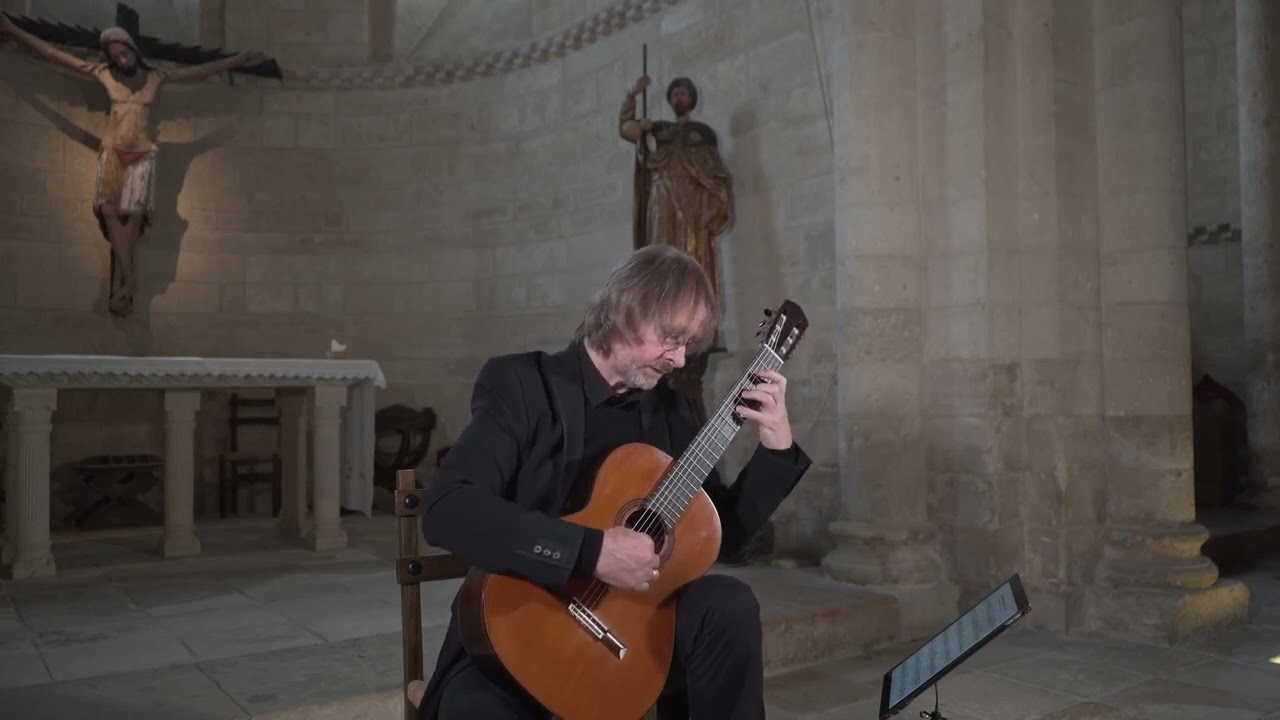
\includegraphics[width=0.48\linewidth]{pictures/youtube/2026/03/20260311_201612_youtube_001_zwzjLeQIokE.jpg}
}
\end{center}

\subsection*{2026年03月11日 20:16}
\addcontentsline{toc}{subsection}{2026年03月11日 20:16}

\paragraph{リンク}
\url{https://youtu.be/TY1tZ5XSzfk}

\begin{center}
\href{https://youtu.be/TY1tZ5XSzfk}{
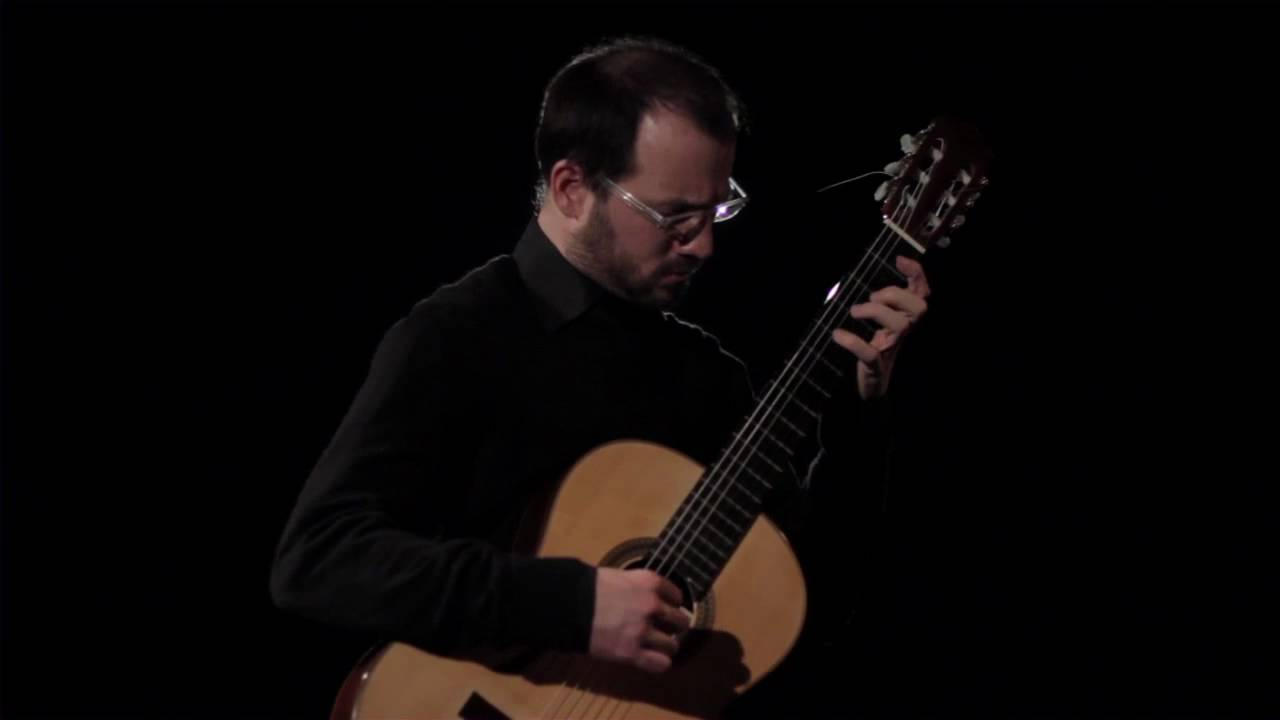
\includegraphics[width=0.48\linewidth]{pictures/youtube/2026/03/20260311_201636_youtube_001_TY1tZ5XSzfk.jpg}
}
\end{center}

\subsection*{2026年03月11日 20:26}
\addcontentsline{toc}{subsection}{2026年03月11日 20:26}

\paragraph{リンク}
\url{https://youtu.be/I-h5WfSBx0o?t=148}

\begin{center}
\href{https://youtu.be/I-h5WfSBx0o?t=148}{
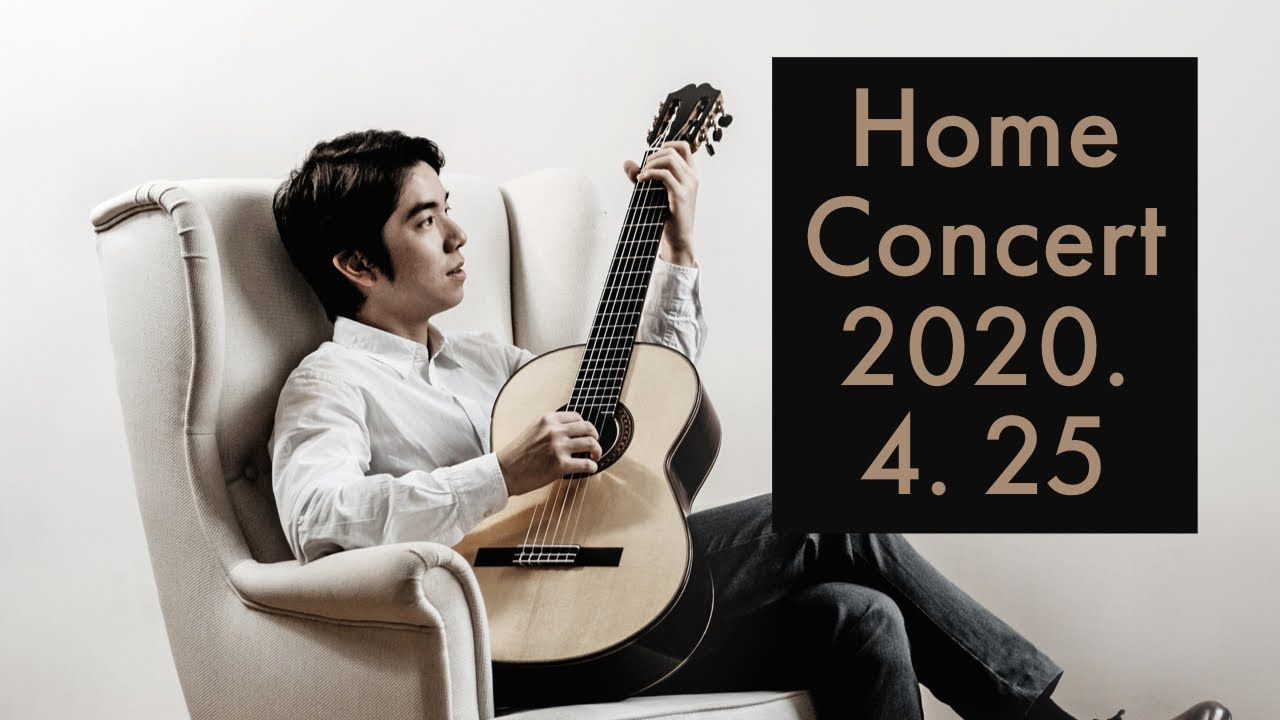
\includegraphics[width=0.48\linewidth]{pictures/youtube/2026/03/20260311_202635_youtube_001_I-h5WfSBx0o.jpg}
}
\end{center}

\subsection*{2026年03月11日 20:46}
\addcontentsline{toc}{subsection}{2026年03月11日 20:46}

\paragraph{リンク}
\url{https://youtu.be/sf9LQ8vpPpQ}

\begin{center}
\href{https://youtu.be/sf9LQ8vpPpQ}{
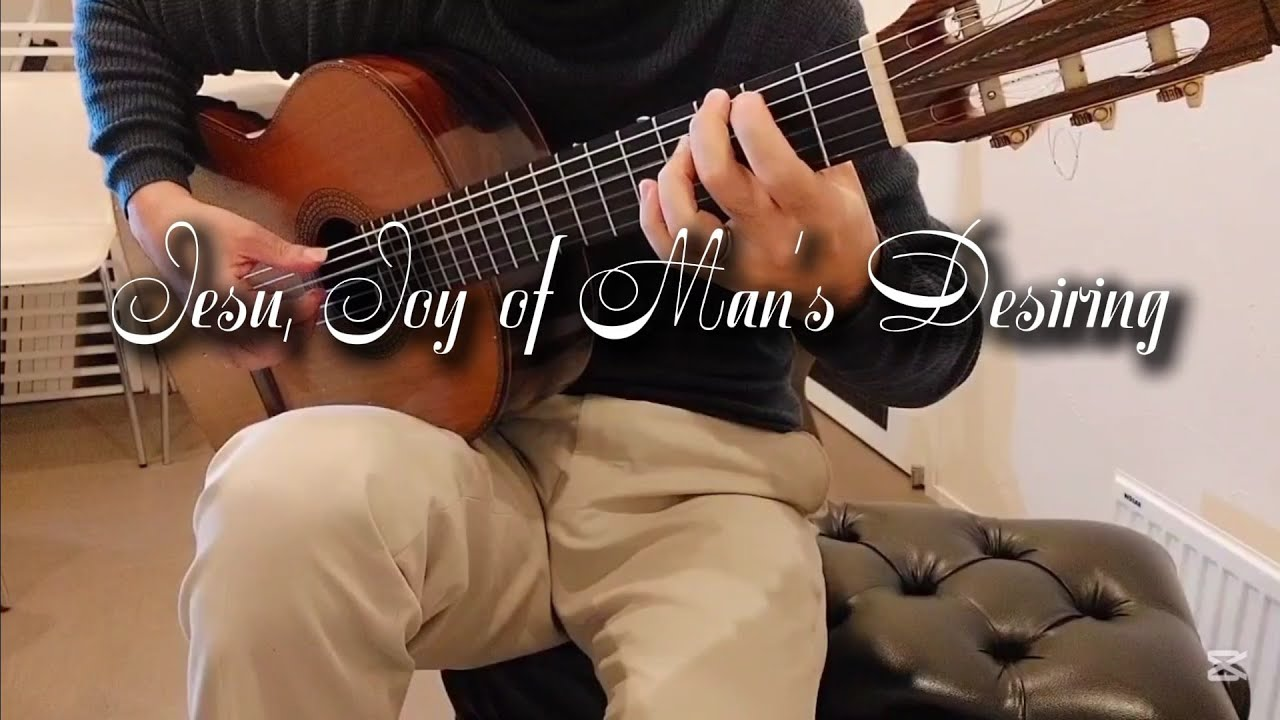
\includegraphics[width=0.48\linewidth]{pictures/youtube/2026/03/20260311_204659_youtube_001_sf9LQ8vpPpQ.jpg}
}
\end{center}

\subsection*{2026年03月12日 00:52}
\addcontentsline{toc}{subsection}{2026年03月12日 00:52}

朝日川柳３月４日「愚か者歴史に韻をまた踏ませ」

「歴史は韻を踏む」は、マーク・トウェイン作とされる英語の格言"History doesn't repeat itself, but it rhymes."（歴史は繰り返さないが、韻を踏む）から。「まったく同じことは起きないが、似たパターンが繰り返される」つまり、愚か者がまたベトナムやイラク、アフガンのような破局的なことに手を出したと警告した川柳。


（「歴史は繰り返さないが、韻を踏む」は、磯田道史氏もNHKの歴史番組でよく口にしていらっしゃるので聞いたことあったけど、マーク・トゥウェインがオリジナルだったとは）

\subsection*{2026年03月12日 03:32}
\addcontentsline{toc}{subsection}{2026年03月12日 03:32}

\paragraph{リンク}
\url{https://youtu.be/wAWJnL71XHo}

\begin{center}
\href{https://youtu.be/wAWJnL71XHo}{
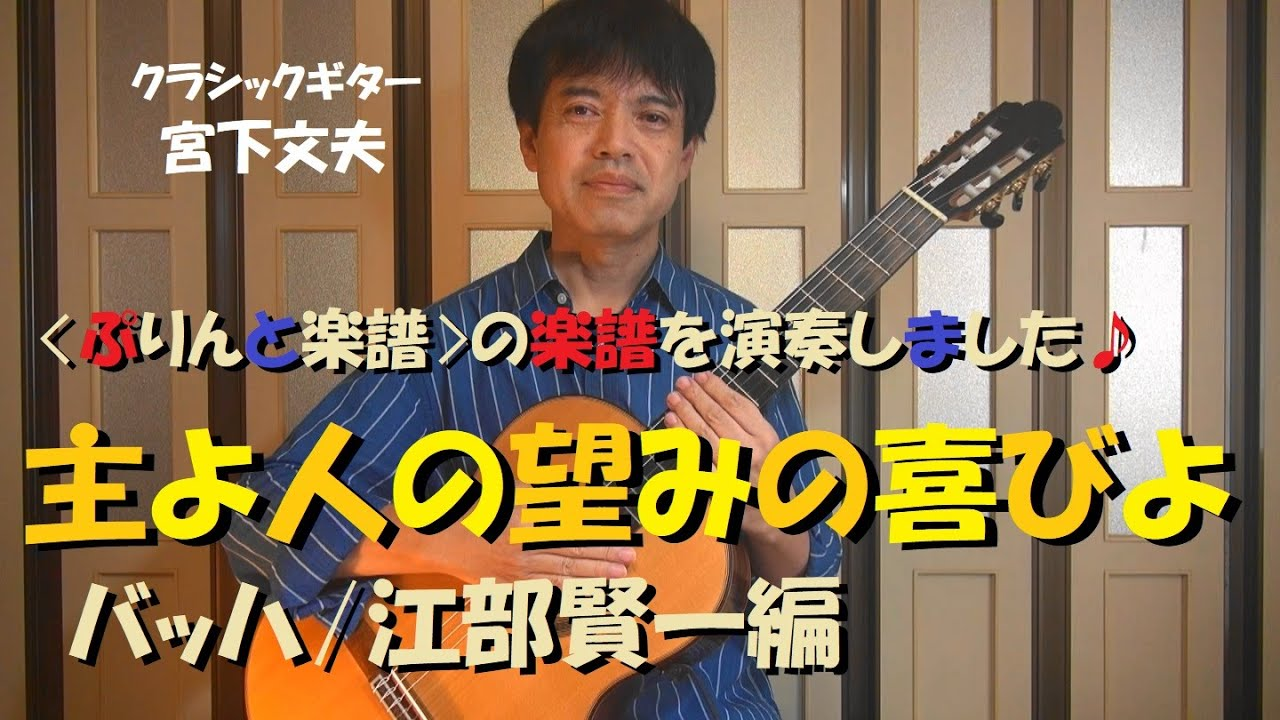
\includegraphics[width=0.48\linewidth]{pictures/youtube/2026/03/20260312_033218_youtube_001_wAWJnL71XHo.jpg}
}
\end{center}

\subsection*{2026年03月12日 22:12}
\addcontentsline{toc}{subsection}{2026年03月12日 22:12}

\paragraph{リンク}
\url{https://youtu.be/dzzWmcI6AXk}

\begin{center}
\href{https://youtu.be/dzzWmcI6AXk}{
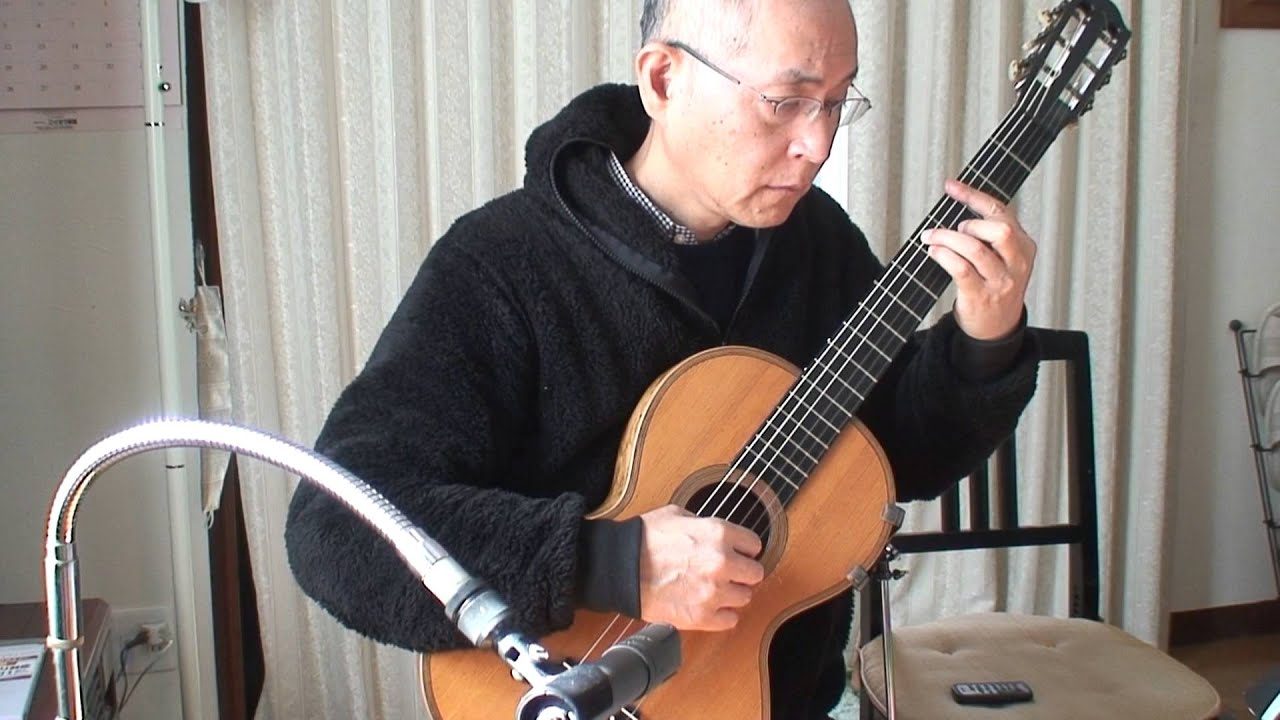
\includegraphics[width=0.48\linewidth]{pictures/youtube/2026/03/20260312_221225_youtube_001_dzzWmcI6AXk.jpg}
}
\end{center}

\subsection*{2026年03月13日 08:57}
\addcontentsline{toc}{subsection}{2026年03月13日 08:57}

\paragraph{リンク}
\url{https://youtu.be/Hw_xQX1M4T0}

\begin{center}
\href{https://youtu.be/Hw_xQX1M4T0}{
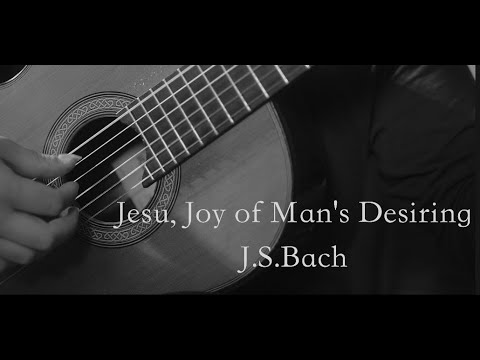
\includegraphics[width=0.48\linewidth]{pictures/youtube/2026/03/20260313_085703_youtube_001_Hw_xQX1M4T0.jpg}
}
\end{center}

\subsection*{2026年03月13日 08:59}
\addcontentsline{toc}{subsection}{2026年03月13日 08:59}

\paragraph{リンク}
\url{https://youtu.be/NBrCa6GXzrU}

\begin{center}
\href{https://youtu.be/NBrCa6GXzrU}{
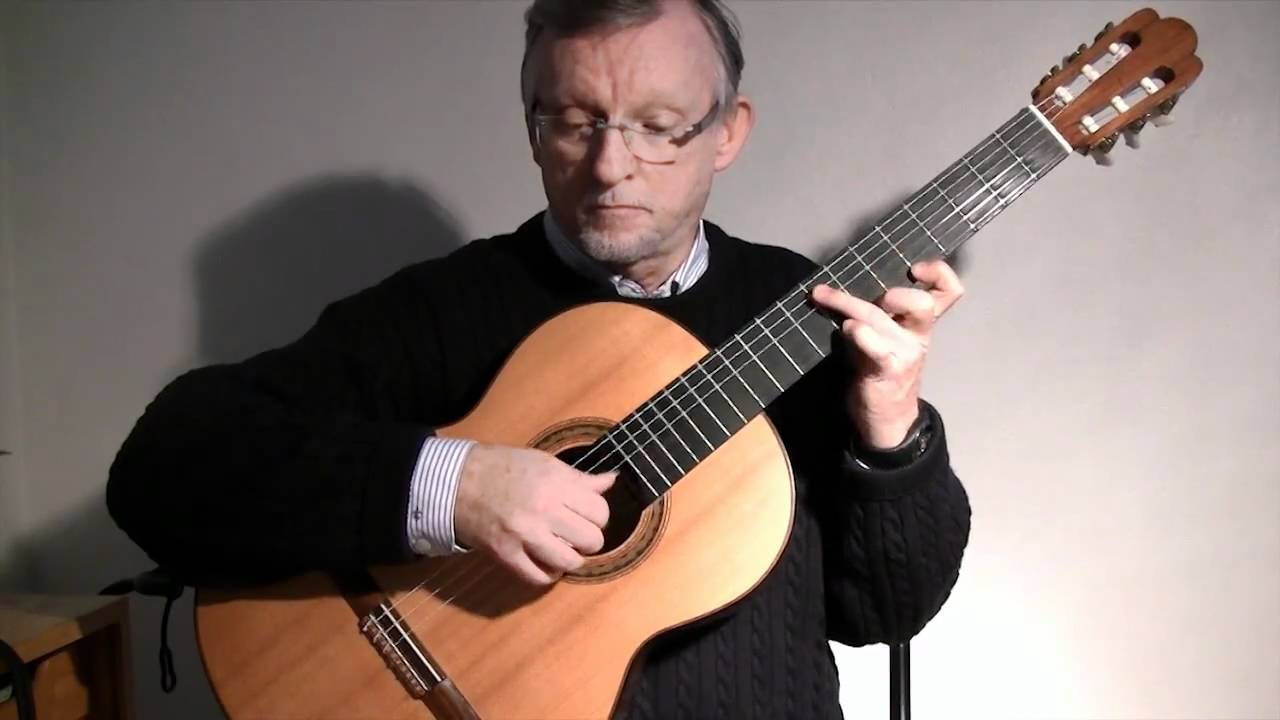
\includegraphics[width=0.48\linewidth]{pictures/youtube/2026/03/20260313_085932_youtube_001_NBrCa6GXzrU.jpg}
}
\end{center}

\subsection*{2026年03月13日 09:00}
\addcontentsline{toc}{subsection}{2026年03月13日 09:00}

\paragraph{リンク}
\url{https://youtu.be/nLVbUvWxV8A}

\begin{center}
\href{https://youtu.be/nLVbUvWxV8A}{
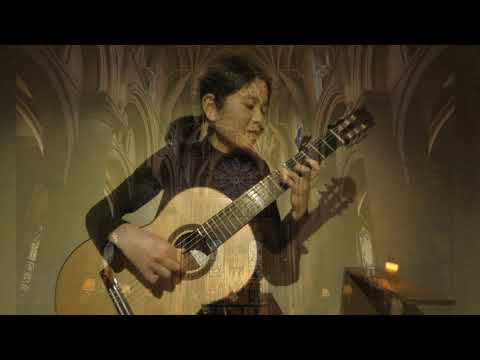
\includegraphics[width=0.48\linewidth]{pictures/youtube/2026/03/20260313_090000_youtube_001_nLVbUvWxV8A.jpg}
}
\end{center}

\subsection*{2026年03月14日 03:22}
\addcontentsline{toc}{subsection}{2026年03月14日 03:22}

\paragraph{リンク}
\url{https://youtu.be/0NapJ_4g7Y0}

\begin{center}
\href{https://youtu.be/0NapJ_4g7Y0}{
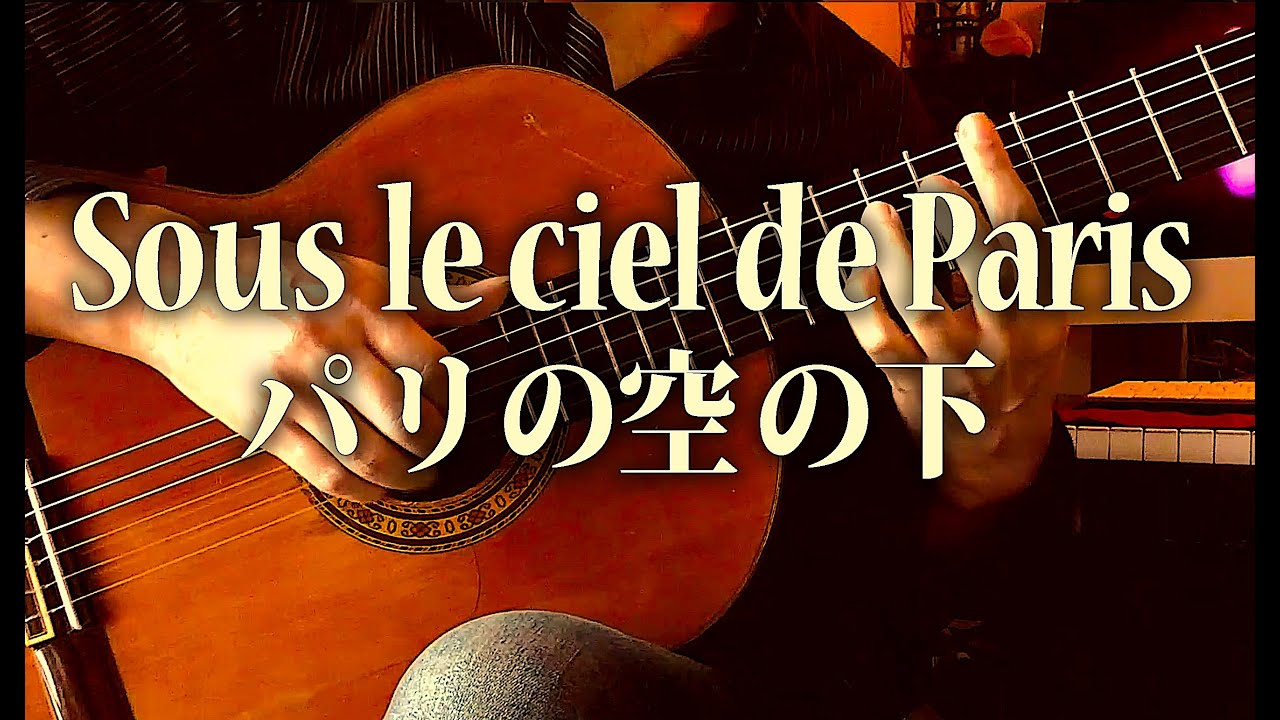
\includegraphics[width=0.48\linewidth]{pictures/youtube/2026/03/20260314_032201_youtube_001_0NapJ_4g7Y0.jpg}
}
\end{center}

\subsection*{2026年03月14日 03:25}
\addcontentsline{toc}{subsection}{2026年03月14日 03:25}

\paragraph{リンク}
\url{https://youtu.be/clwk_SREThg}

\begin{center}
\href{https://youtu.be/clwk_SREThg}{
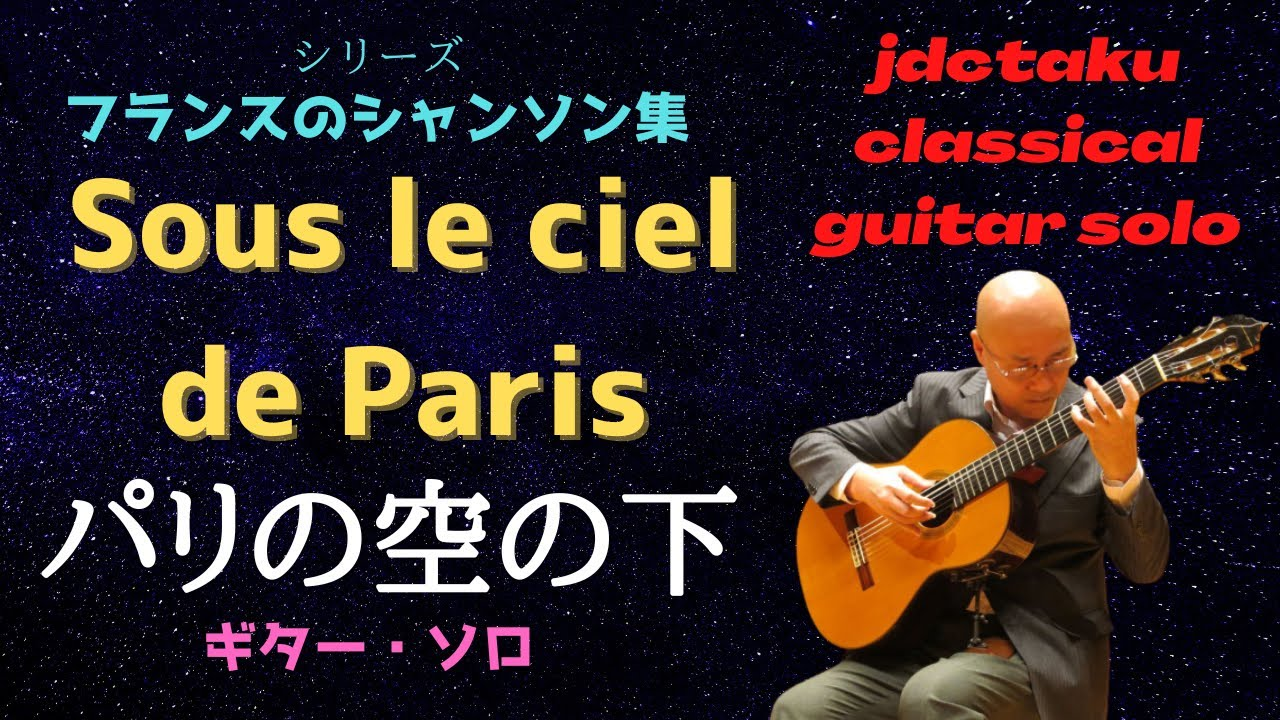
\includegraphics[width=0.48\linewidth]{pictures/youtube/2026/03/20260314_032537_youtube_001_clwk_SREThg.jpg}
}
\end{center}

\subsection*{2026年03月14日 03:52}
\addcontentsline{toc}{subsection}{2026年03月14日 03:52}

\paragraph{リンク}
\url{https://youtu.be/i2SNAhdy5B4}

\begin{center}
\href{https://youtu.be/i2SNAhdy5B4}{
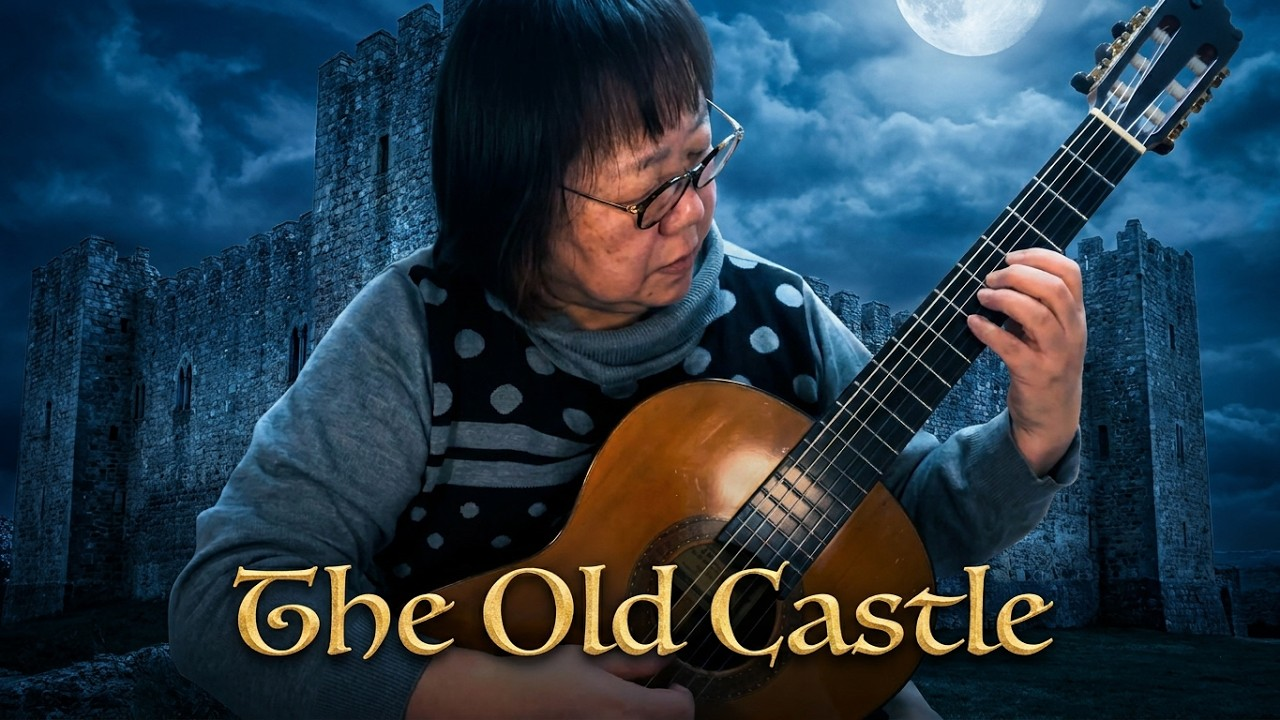
\includegraphics[width=0.48\linewidth]{pictures/youtube/2026/03/20260314_035242_youtube_001_i2SNAhdy5B4.jpg}
}
\end{center}

\subsection*{2026年03月15日 00:48}
\addcontentsline{toc}{subsection}{2026年03月15日 00:48}

BWV1002 Violin Partita No,1 より Sarabande


リョベートがバッハを編曲していた？

\url{https://youtu.be/fQUgEKWuuTs}

\begin{center}
\href{https://youtu.be/fQUgEKWuuTs}{
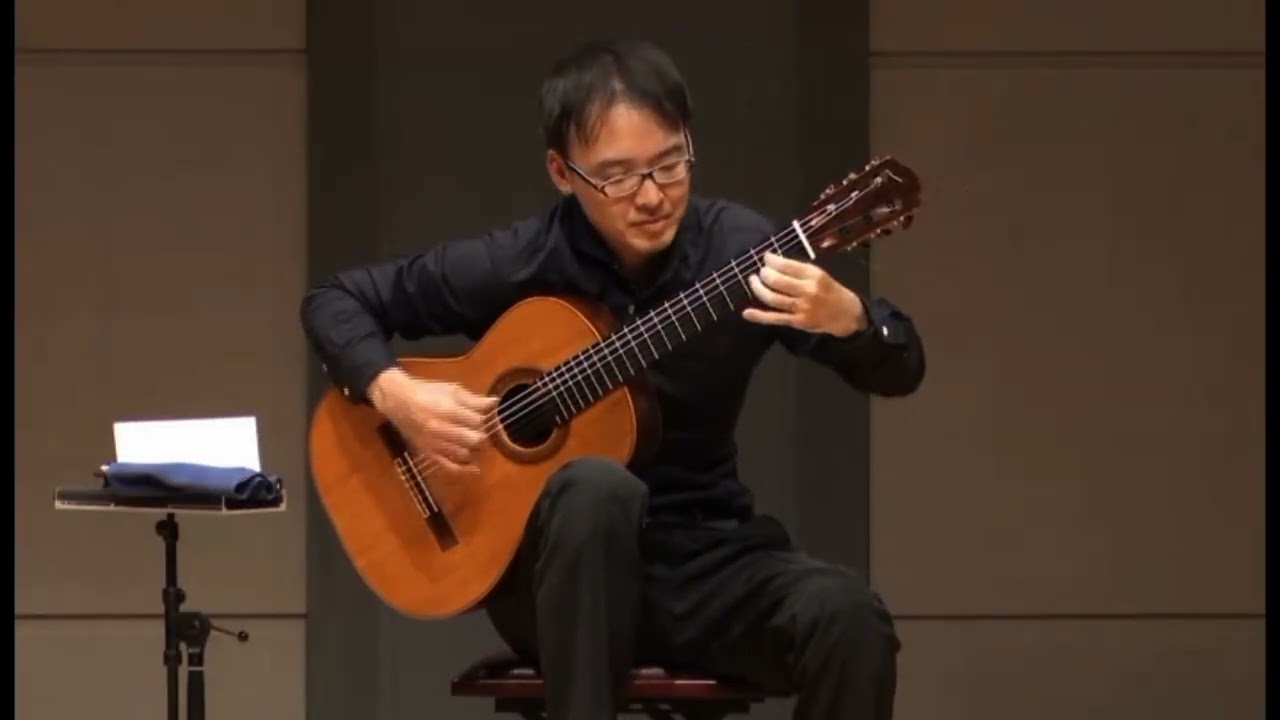
\includegraphics[width=0.48\linewidth]{pictures/youtube/2026/03/20260315_004803_youtube_001_fQUgEKWuuTs.jpg}
}
\end{center}



「セゴヴィアと親交のあった（タレガの高弟である）ミゲル・リョベートは、そのレパートリーの中にBWV1002のサラバンドを入れていた」という様な記述が、菅原潤 氏による前書き部（ホマ・ドリーム社刊によるセゴヴィア・レパートリーVol.8）に書かれている（けど、この楽譜集にBWV1002のSarabandeは載っていない）


田部井辰雄氏は、これ↓は「セゴヴィア編による演奏を基にした」と仰っています

\url{https://youtu.be/KOl36rcS2sA}

\begin{center}
\href{https://youtu.be/KOl36rcS2sA}{
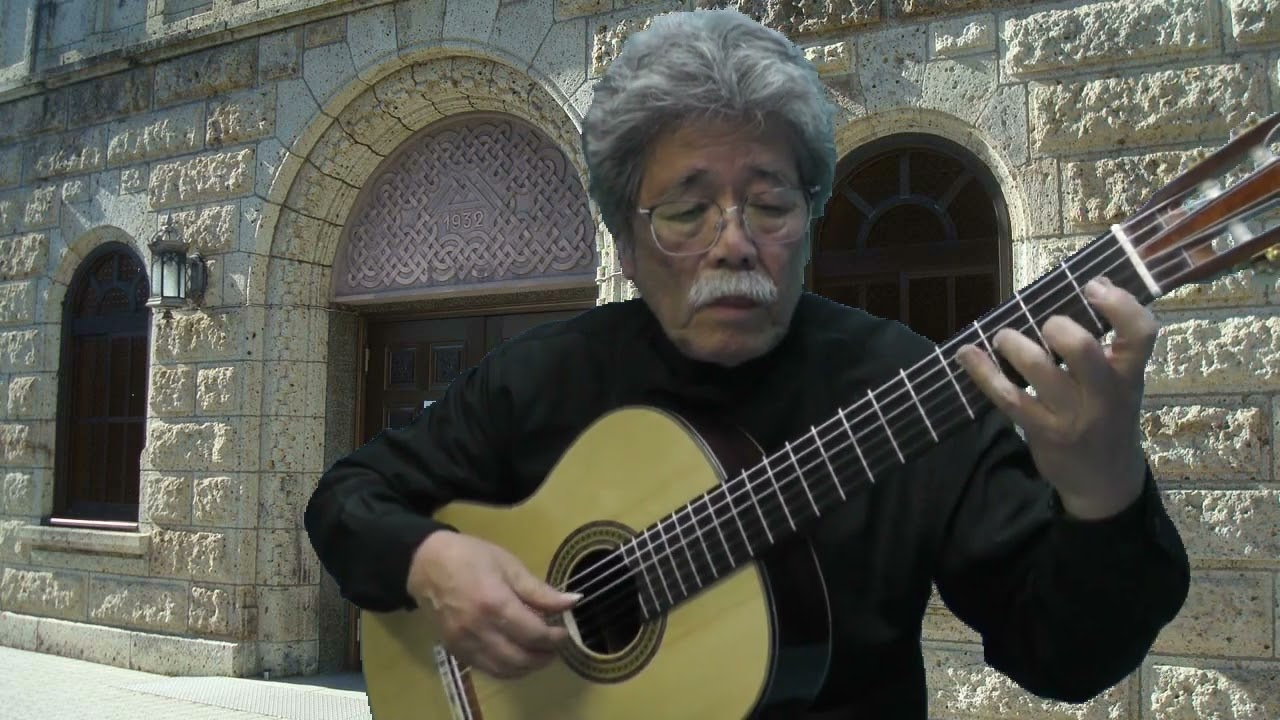
\includegraphics[width=0.48\linewidth]{pictures/youtube/2026/03/20260315_004803_youtube_002_KOl36rcS2sA.jpg}
}
\end{center}




この方↓は、「原曲のヴァイオリン譜の音を、そのままギターで演奏しました(\textasciicircum{}\textasciicircum{}♪」と仰っています

\url{https://youtu.be/169B7IgLhp0}

\begin{center}
\href{https://youtu.be/169B7IgLhp0}{
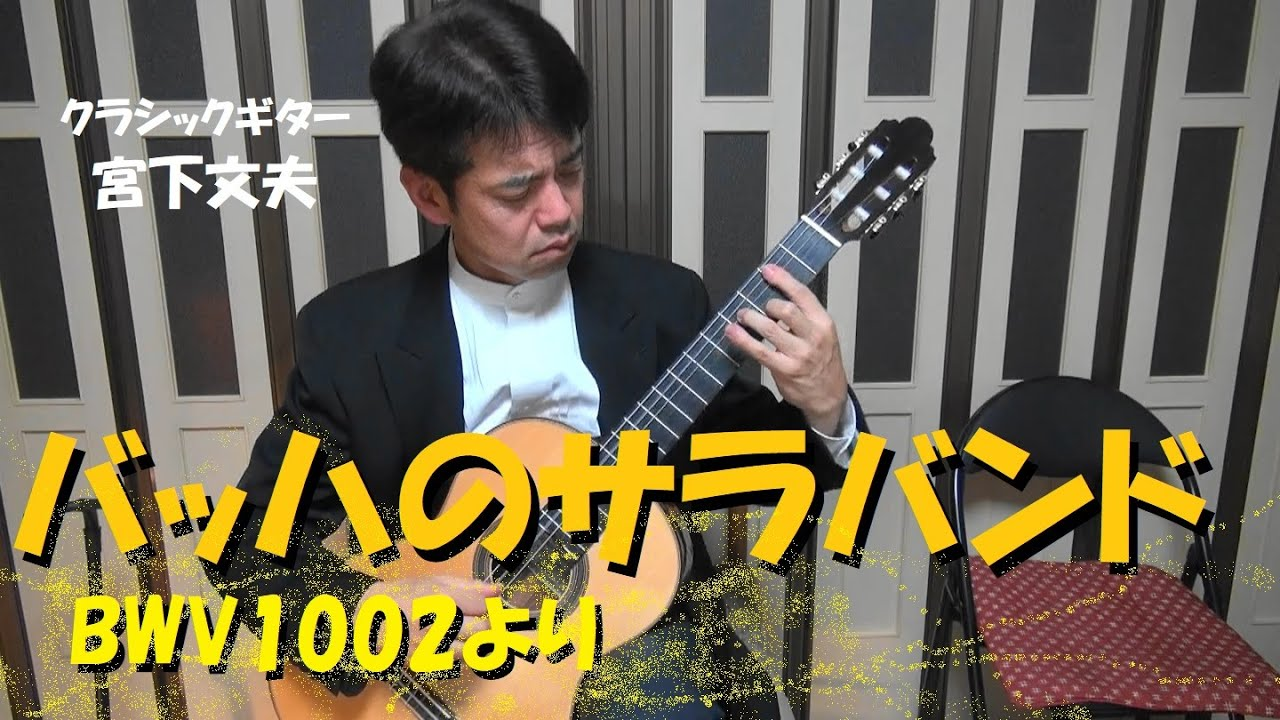
\includegraphics[width=0.48\linewidth]{pictures/youtube/2026/03/20260315_004803_youtube_003_169B7IgLhp0.jpg}
}
\end{center}




セルシェル 氏も、keyを変えただけだ（base音もちょっと加えてみたけど）「I basically play the original just in another key. And with a few low base notes that I could not regist adding.」などと仰っています（in another keyになっているのかな？←他の方の演奏と同じkeyの様な気がする）

\url{https://youtu.be/6-oAFbHt1oM}

\begin{center}
\href{https://youtu.be/6-oAFbHt1oM}{
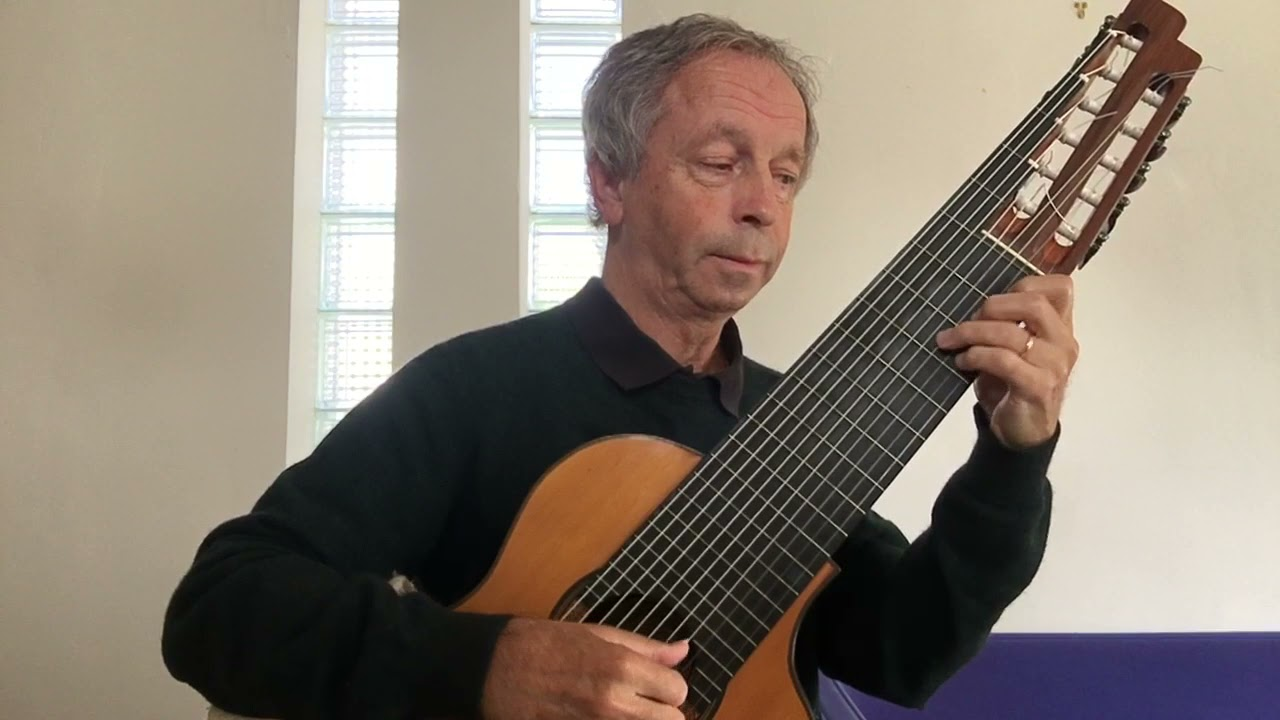
\includegraphics[width=0.48\linewidth]{pictures/youtube/2026/03/20260315_004803_youtube_004_6-oAFbHt1oM.jpg}
}
\end{center}




この方↓も、ヴァイオリンの楽譜のままだ（繰り返しでちょっと変えたけど）「I just worked it out directly from the violin score and made some embellishments（←装飾） in the repeats. 」と（コメント欄で）仰っています

\url{https://youtu.be/szgA_5hrNjA}

\begin{center}
\href{https://youtu.be/szgA_5hrNjA}{
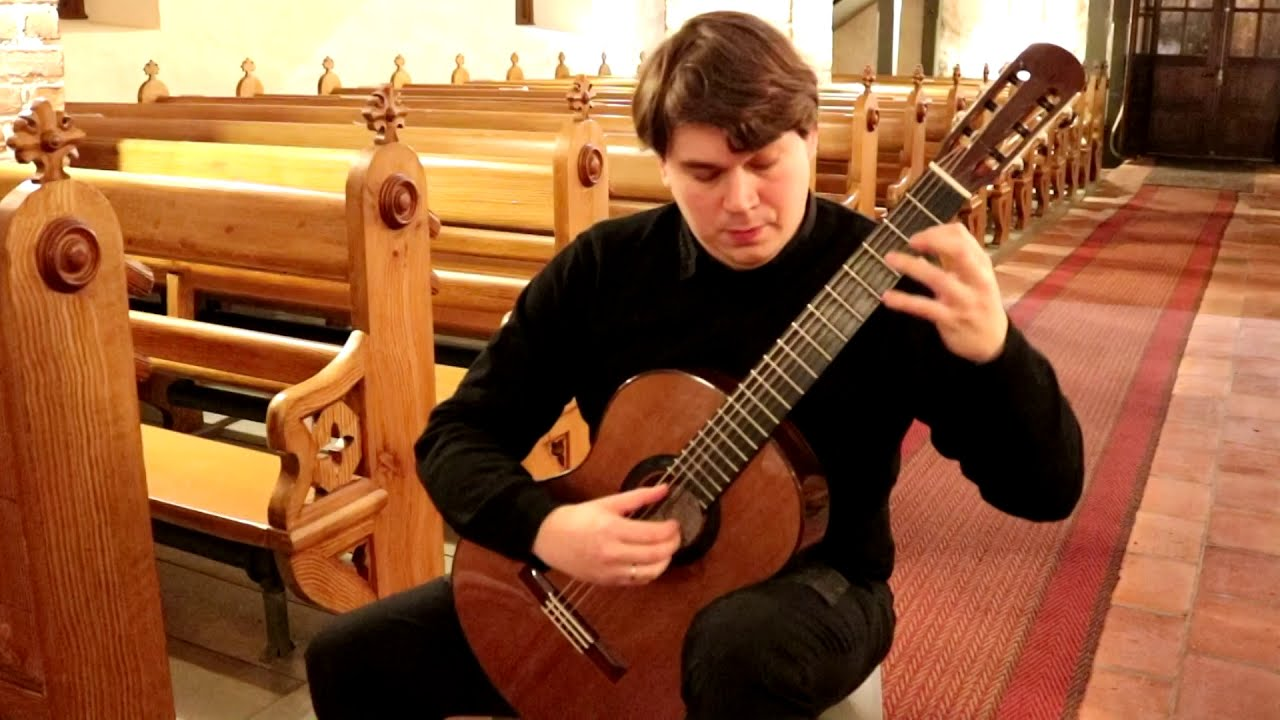
\includegraphics[width=0.48\linewidth]{pictures/youtube/2026/03/20260315_004803_youtube_005_szgA_5hrNjA.jpg}
}
\end{center}



因みにこの方↑こそ、keyはバロックピッチ（A=415Hz）で弾いていらっしゃるのでは？


こちら↓は誰の編曲とも仰っていませんね

\url{https://youtu.be/m09QU-ci9Og}

\begin{center}
\href{https://youtu.be/m09QU-ci9Og}{
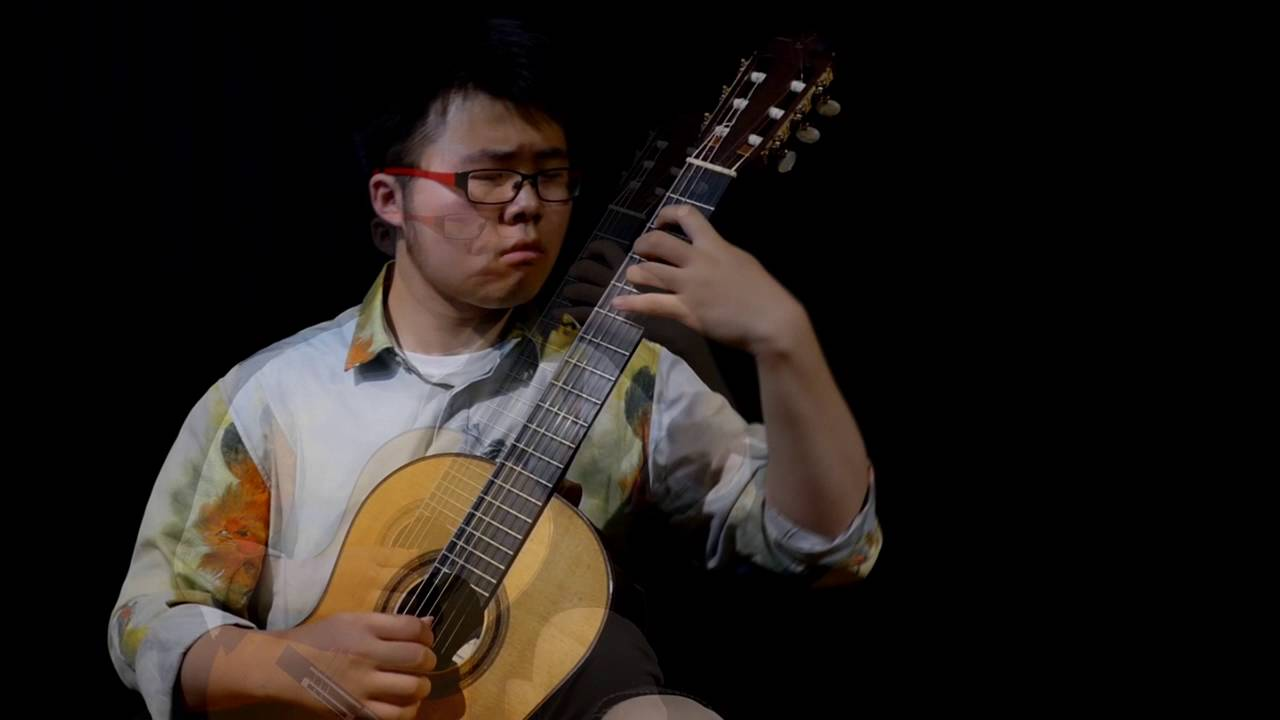
\includegraphics[width=0.48\linewidth]{pictures/youtube/2026/03/20260315_004803_youtube_006_m09QU-ci9Og.jpg}
}
\end{center}




演奏に編曲者名が現れない事が多い様に見えるのは、ほぼ原曲通りだからなのかもしれません


Partitaの1番 BWV1002は、Allemand-Corrente-Sarabande-BoreaのそれぞれにDouble （ドゥーブル）という変奏部が付属する構造になっていることから、実際の演奏では、Sarabandeの後にDoubleを続けた格好で演奏される事もある様です。

\url{https://youtu.be/dMBNu6i0cQI}

\begin{center}
\href{https://youtu.be/dMBNu6i0cQI}{
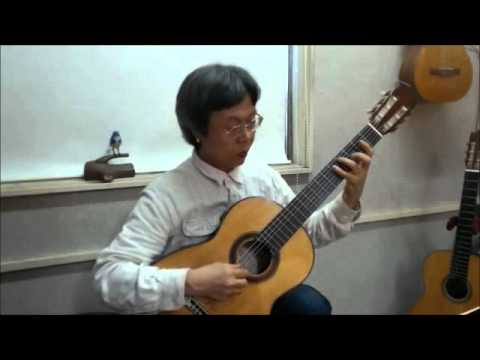
\includegraphics[width=0.48\linewidth]{pictures/youtube/2026/03/20260315_004803_youtube_007_dMBNu6i0cQI.jpg}
}
\end{center}



\url{https://youtu.be/KOl36rcS2sA}



この方↓、Sarabandeはちょっと勿体ぶっている様にも聞こえるけど、Doubleの方はイタズラに速くなくて良い様な気がします。

\url{https://youtu.be/m9ivovfIFIM}

\begin{center}
\href{https://youtu.be/m9ivovfIFIM}{
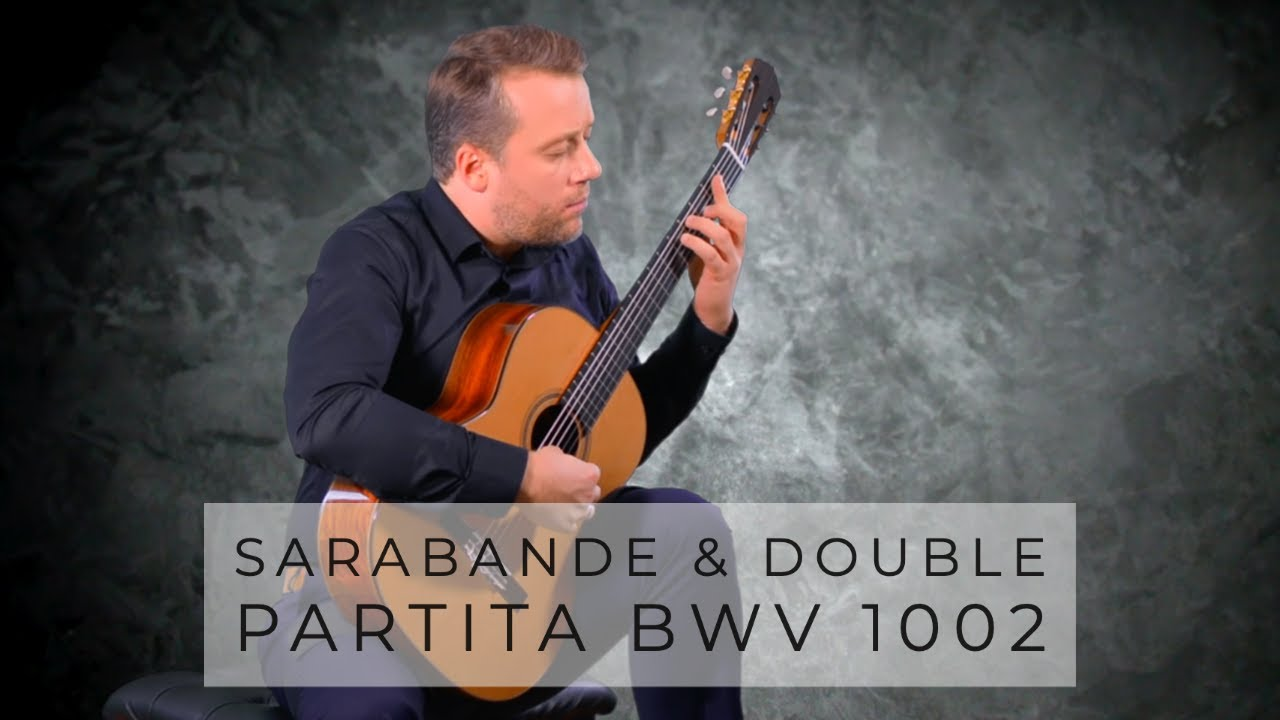
\includegraphics[width=0.48\linewidth]{pictures/youtube/2026/03/20260315_004803_youtube_008_m9ivovfIFIM.jpg}
}
\end{center}




（それにしても、セゴヴィア編によるSarabandeの楽譜ってどこにある？私はリョベート編もセゴヴィア編も手元にありません）


さてViolinソロによるオリジナルなら、例えばヒラリー・ハーンなどは如何でしょう（アンコール用なのか？Youtubeには、この方によるこの曲の演奏動画がアレコレ出てきますネ）

\url{https://youtu.be/5XzZudf5LJ0}

\begin{center}
\href{https://youtu.be/5XzZudf5LJ0}{
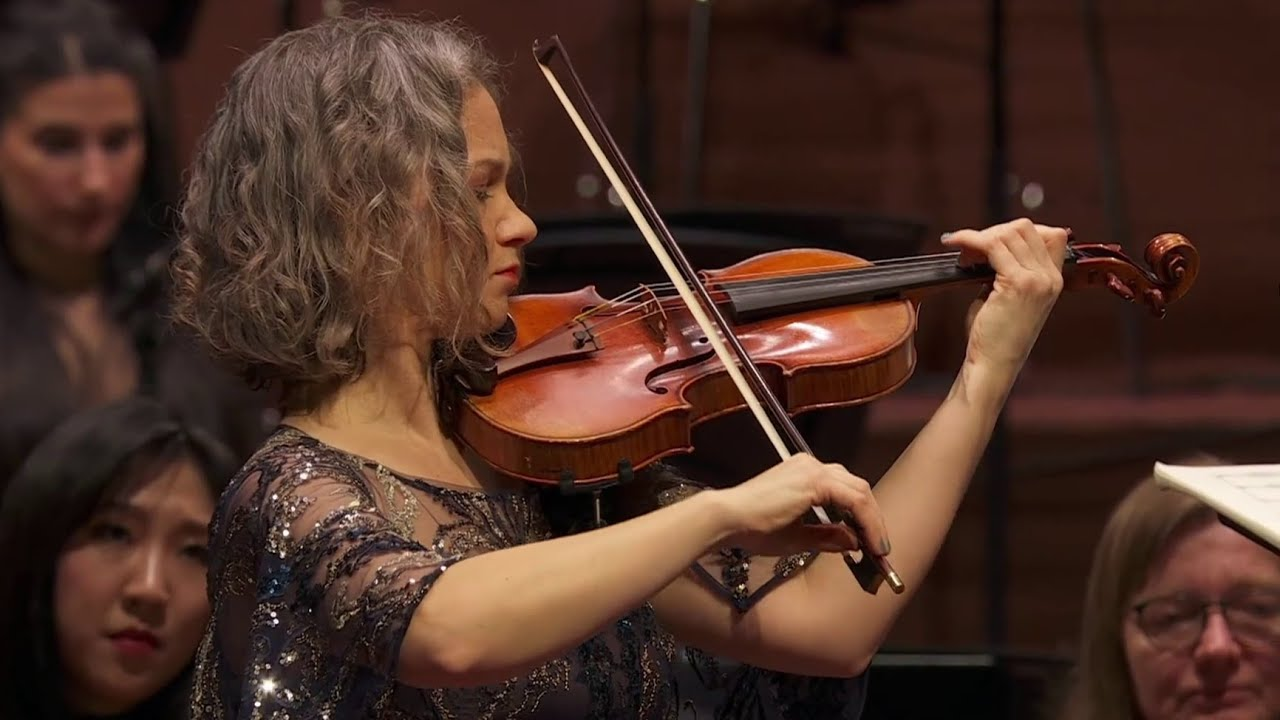
\includegraphics[width=0.48\linewidth]{pictures/youtube/2026/03/20260315_004803_youtube_009_5XzZudf5LJ0.jpg}
}
\end{center}



\url{https://youtu.be/SKDo31z6U1E}

\begin{center}
\href{https://youtu.be/SKDo31z6U1E}{
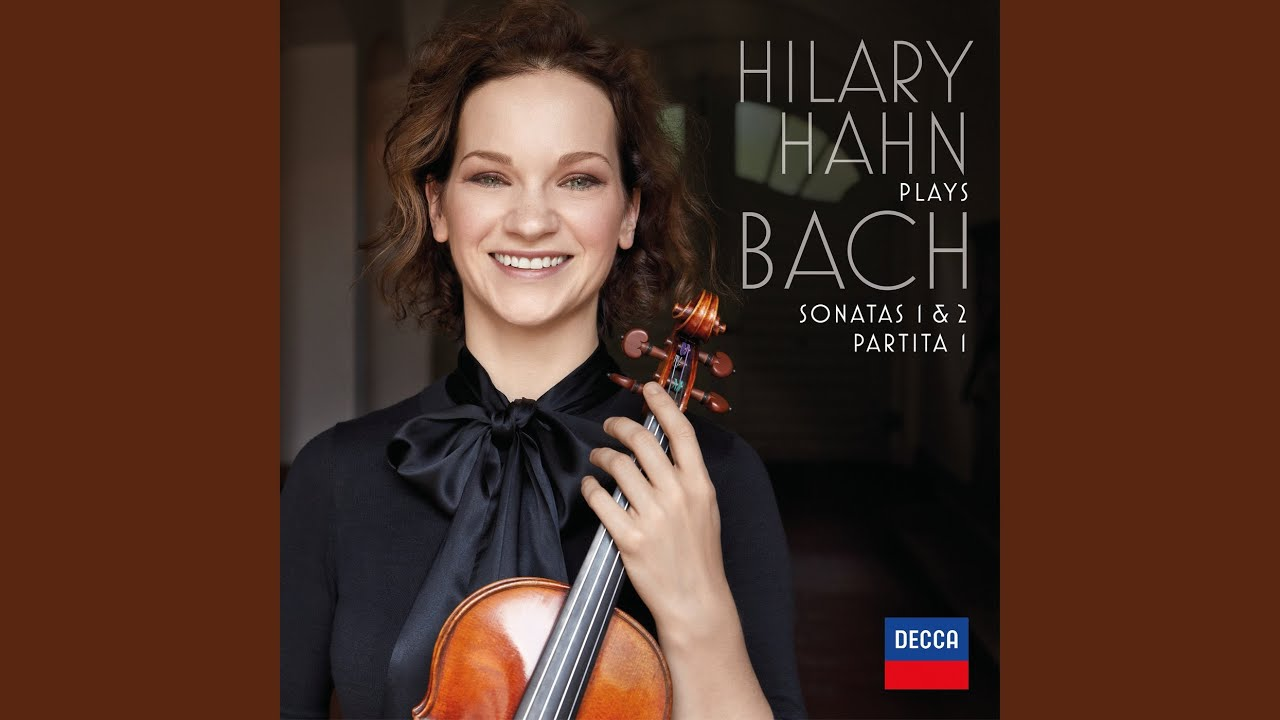
\includegraphics[width=0.48\linewidth]{pictures/youtube/2026/03/20260315_004803_youtube_010_SKDo31z6U1E.jpg}
}
\end{center}




===

バッハのギター曲一覧はここ

\url{https://m.facebook.com/story.php?story_fbid=25468465252810962&id=100002225117991}



\subsection*{2026年03月15日 02:21}
\addcontentsline{toc}{subsection}{2026年03月15日 02:21}

\paragraph{リンク}
\url{https://youtu.be/szgA_5hrNjA}

\begin{center}
\href{https://youtu.be/szgA_5hrNjA}{
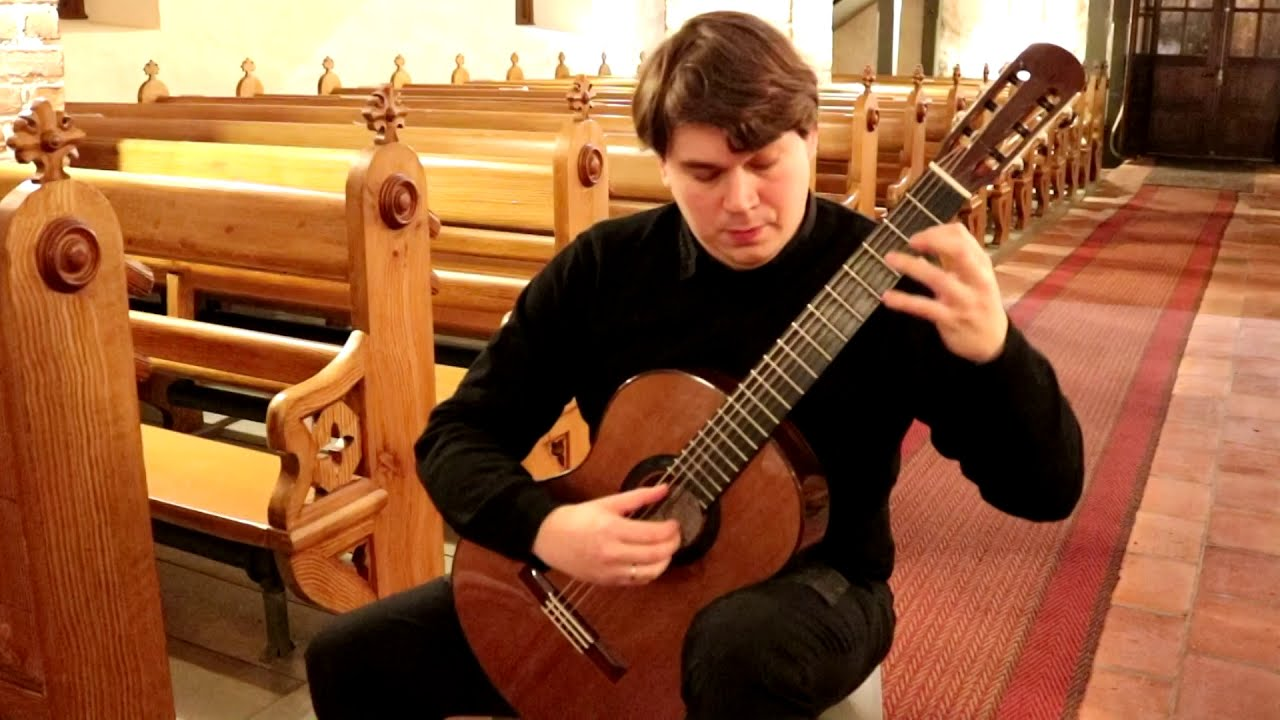
\includegraphics[width=0.48\linewidth]{pictures/youtube/2026/03/20260315_022112_youtube_001_szgA_5hrNjA.jpg}
}
\end{center}

\subsection*{2026年03月15日 05:27}
\addcontentsline{toc}{subsection}{2026年03月15日 05:27}

\paragraph{リンク}
\url{https://youtu.be/KgSKvOAJMb8}

\begin{center}
\href{https://youtu.be/KgSKvOAJMb8}{
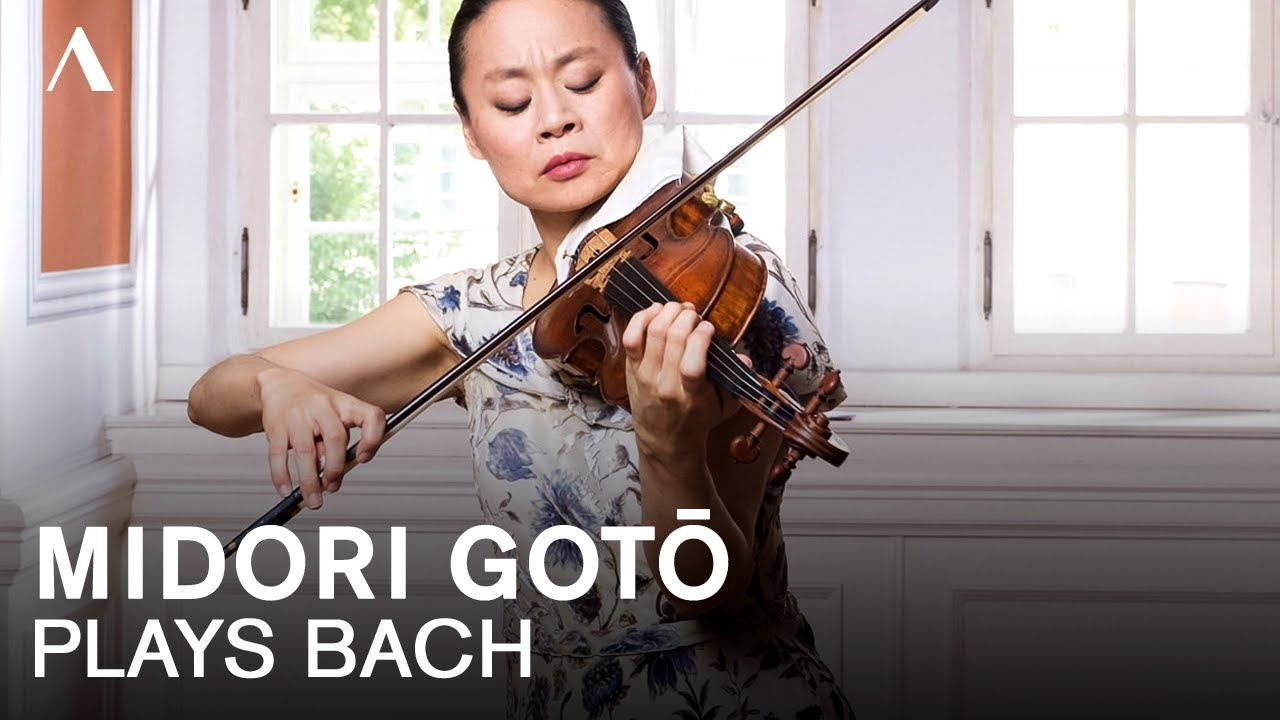
\includegraphics[width=0.48\linewidth]{pictures/youtube/2026/03/20260315_052705_youtube_001_KgSKvOAJMb8.jpg}
}
\end{center}

\subsection*{2026年03月15日 14:51}
\addcontentsline{toc}{subsection}{2026年03月15日 14:51}

Prelude, Fuga （and Allegro）をこれまで凡そ２年ほど練習してきた(もちろん色々よそ見はあった)が、最近のFugaの状況が、ほとんど進歩しなくなってきた。心理学における、いわゆる成長曲線で考えてみると、１つのプラトーに居るとは思うのだが、次のステップに向かう一種のスランプ状態ではないかと（自分勝手に）分析している。

でもここに来て、他の曲に移ろうかと心移りしはじめている。と言うのも、最近以下の、J.S.Bachによる「優しい」3曲が気になっているからなのです。（本当ならば、プラトーから抜け出すには、スランプ状態にあっても苦しいながらももがき続けている必要があるとは思うのだけど）


J.S.Bachによる「優しい」曲３つ（易しくはない）


(１)BWV1012：チェロ組曲６番よりサラバンド

\url{https://www.facebook.com/100002225117991/posts/24986489807675178/}




(２)BWV1002：バイオリン パルティータ１番よりサラバンド

\url{https://www.facebook.com/100002225117991/posts/26074775385513276/}




(３)BWV1005：バイオリン ソナタ３番よりラルゴ

\url{https://www.facebook.com/100002225117991/posts/24629723393351823/}




Prelude Fuga （and Allegro）のFugaが長かったので、その反動からか、とにかく先ずは短い曲に取り組みたいと思っている（上は短い順に並べたつもり）この順でやってみようかな（さてさて、誰の編曲譜に取り組もうか）


===

バッハのギター曲一覧はここ

\url{https://m.facebook.com/story.php?story_fbid=25468465252810962&id=100002225117991}



\subsection*{2026年03月16日 00:08}
\addcontentsline{toc}{subsection}{2026年03月16日 00:08}

ララルー（ディズニー・わんわん物語）


\url{https://youtu.be/ZSFZhjFFgoM}

\begin{center}
\href{https://youtu.be/ZSFZhjFFgoM}{
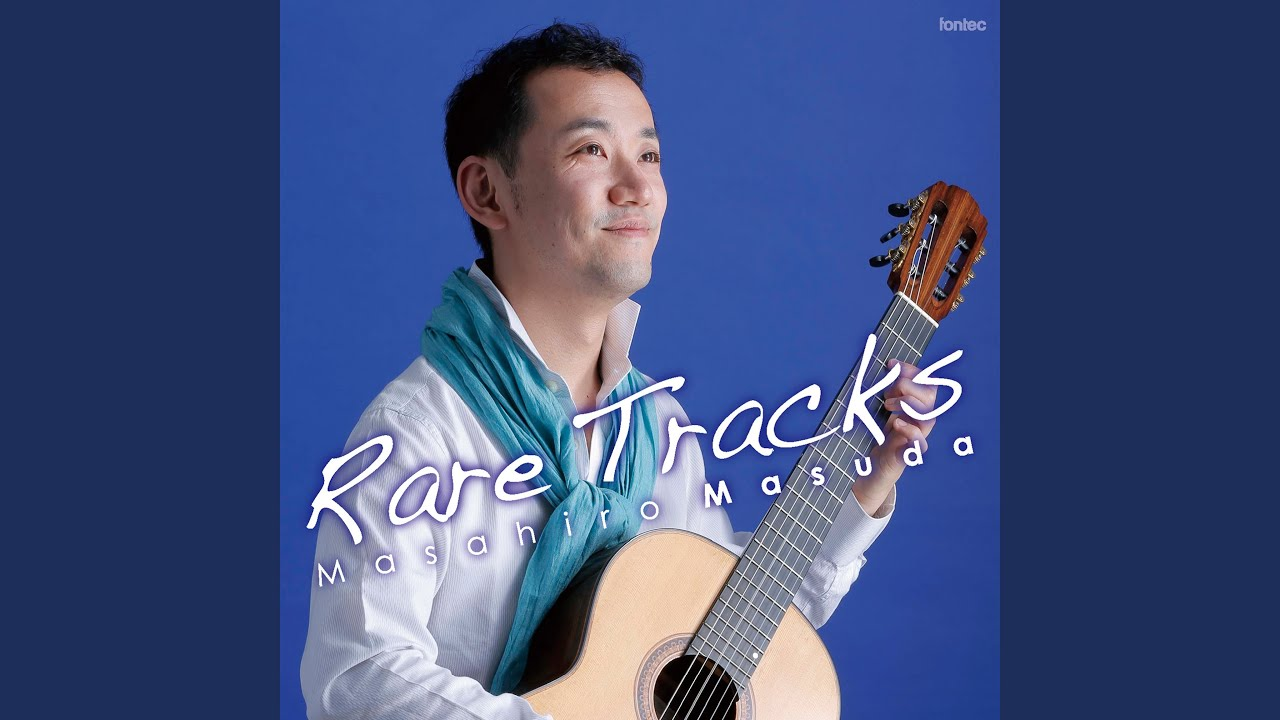
\includegraphics[width=0.48\linewidth]{pictures/youtube/2026/03/20260316_000832_youtube_001_ZSFZhjFFgoM.jpg}
}
\end{center}



編曲は、江部賢一

楽譜は、

\url{https://www.gendaiguitar.com/products/4947817252856}




flute

\url{https://youtu.be/klfXhSKJrRU}

\begin{center}
\href{https://youtu.be/klfXhSKJrRU}{
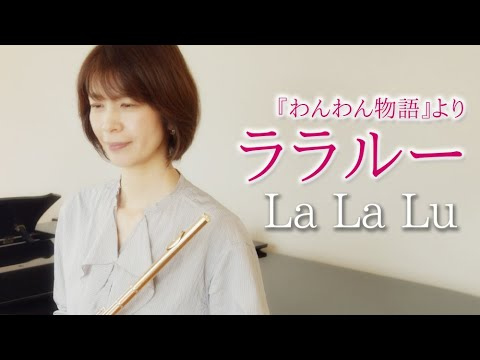
\includegraphics[width=0.48\linewidth]{pictures/youtube/2026/03/20260316_000832_youtube_002_klfXhSKJrRU.jpg}
}
\end{center}



\subsection*{2026年03月17日 05:22}
\addcontentsline{toc}{subsection}{2026年03月17日 05:22}

無伴奏チェロ組曲第６番 Prelude


この曲、これまでの印象では、もっとガツガツしてボウイングのアクセントがガサガサと鳴るチョット乱暴な（？）感じの演奏をよく聞いてきた様に思います。

しかし、この演奏は違います。この淡々と落ち着いた佇まい、静かだが力強い演奏は、とても上品で素敵です（藤原真理氏、さすがと言う他ありません）

\url{https://youtu.be/zdcSSxXSCYU}

\begin{center}
\href{https://youtu.be/zdcSSxXSCYU}{
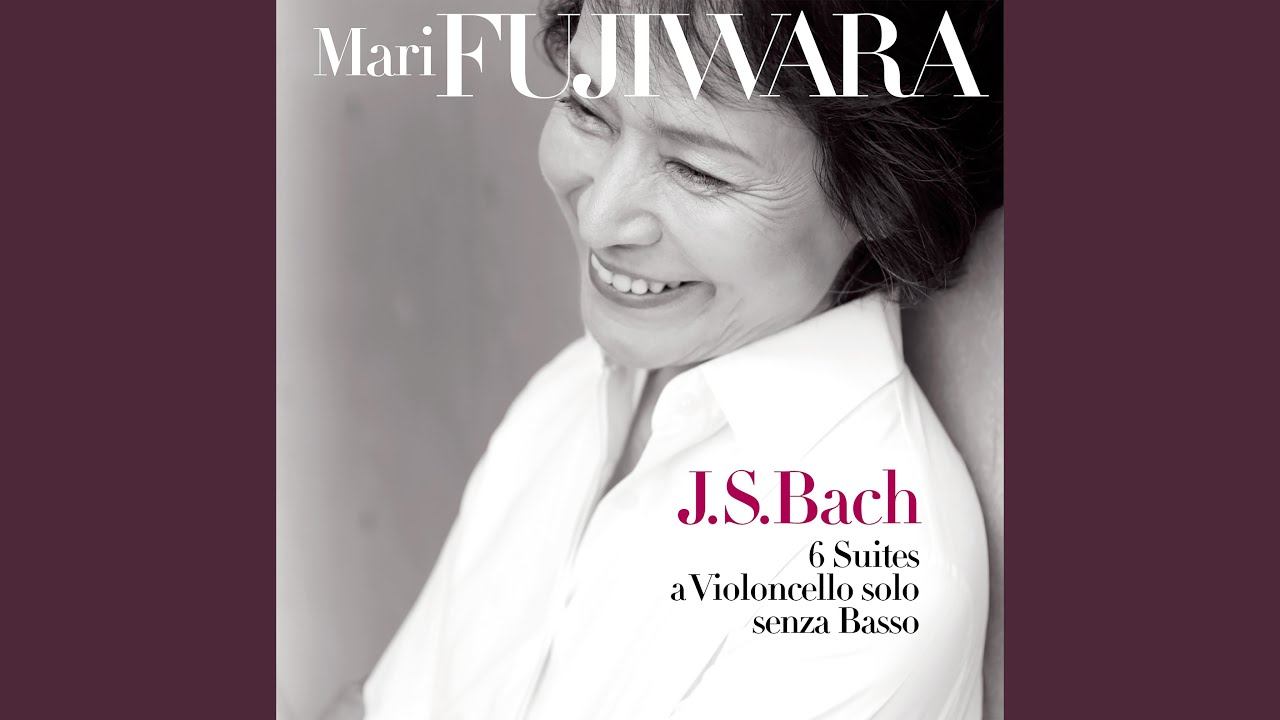
\includegraphics[width=0.48\linewidth]{pictures/youtube/2026/03/20260317_052218_youtube_001_zdcSSxXSCYU.jpg}
}
\end{center}




全曲アルバムはこれ↓（ジャケットは氏の素敵な表情を捉えています）

\url{https://youtube.com/playlist?list=OLAK5uy_leeMiaXzCKBnZmxTXwYJvup0nZjqDVeSY}




藤原真理氏のお若い頃（録音：1982年-1984年）のチェロ組曲のCDを持っています。当時のCDの演奏とは変わってきているのでしょうね。


====

無伴奏フルートの場合

\url{https://youtu.be/m2_atAFCH6I}

\begin{center}
\href{https://youtu.be/m2_atAFCH6I}{
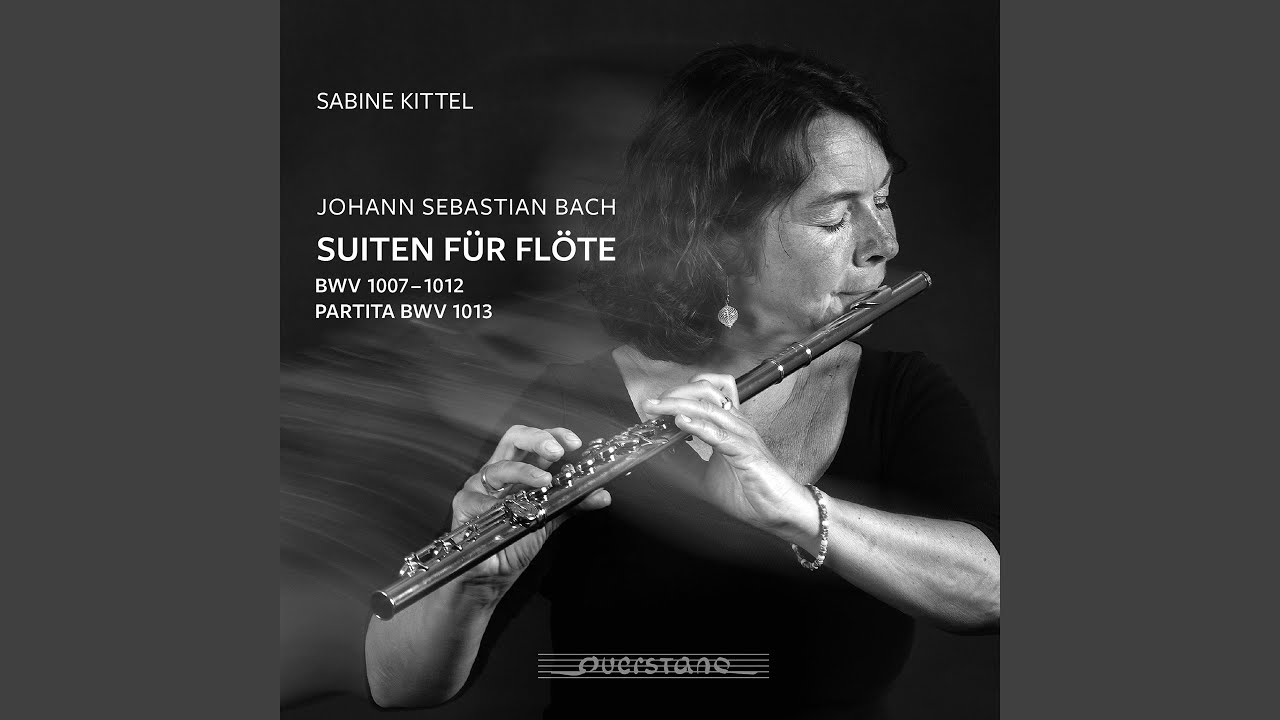
\includegraphics[width=0.48\linewidth]{pictures/youtube/2026/03/20260317_052218_youtube_002_m2_atAFCH6I.jpg}
}
\end{center}



藤井香織氏のチェロ組曲全曲のフルート独奏は衝撃的だったなあ

\url{https://m.facebook.com/story.php?story_fbid=24232785103045656&id=100002225117991}




ギターで弾けたらいいな

\url{https://youtu.be/-QiAsYR8kDQ}

\begin{center}
\href{https://youtu.be/-QiAsYR8kDQ}{
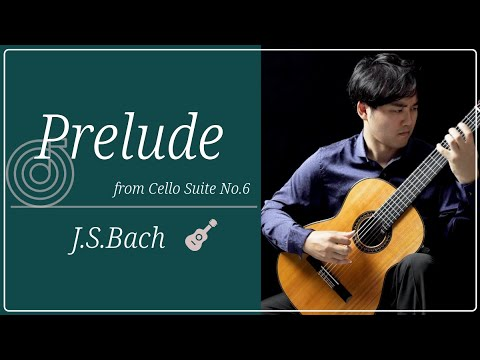
\includegraphics[width=0.48\linewidth]{pictures/youtube/2026/03/20260317_052218_youtube_003_-QiAsYR8kDQ.jpg}
}
\end{center}




ギターの様な「撥弦」楽器では表現し切れない音楽が、チェロやヴァイオリンなどには有りますね。藤原真理氏の音楽を聞いていると、つくづくそう思えてきますよ。


===

バッハのギター曲一覧はここ

\url{https://m.facebook.com/story.php?story_fbid=25468465252810962&id=100002225117991}



\paragraph{写真}
\begin{center}
\begin{minipage}{0.48\linewidth}
\centering
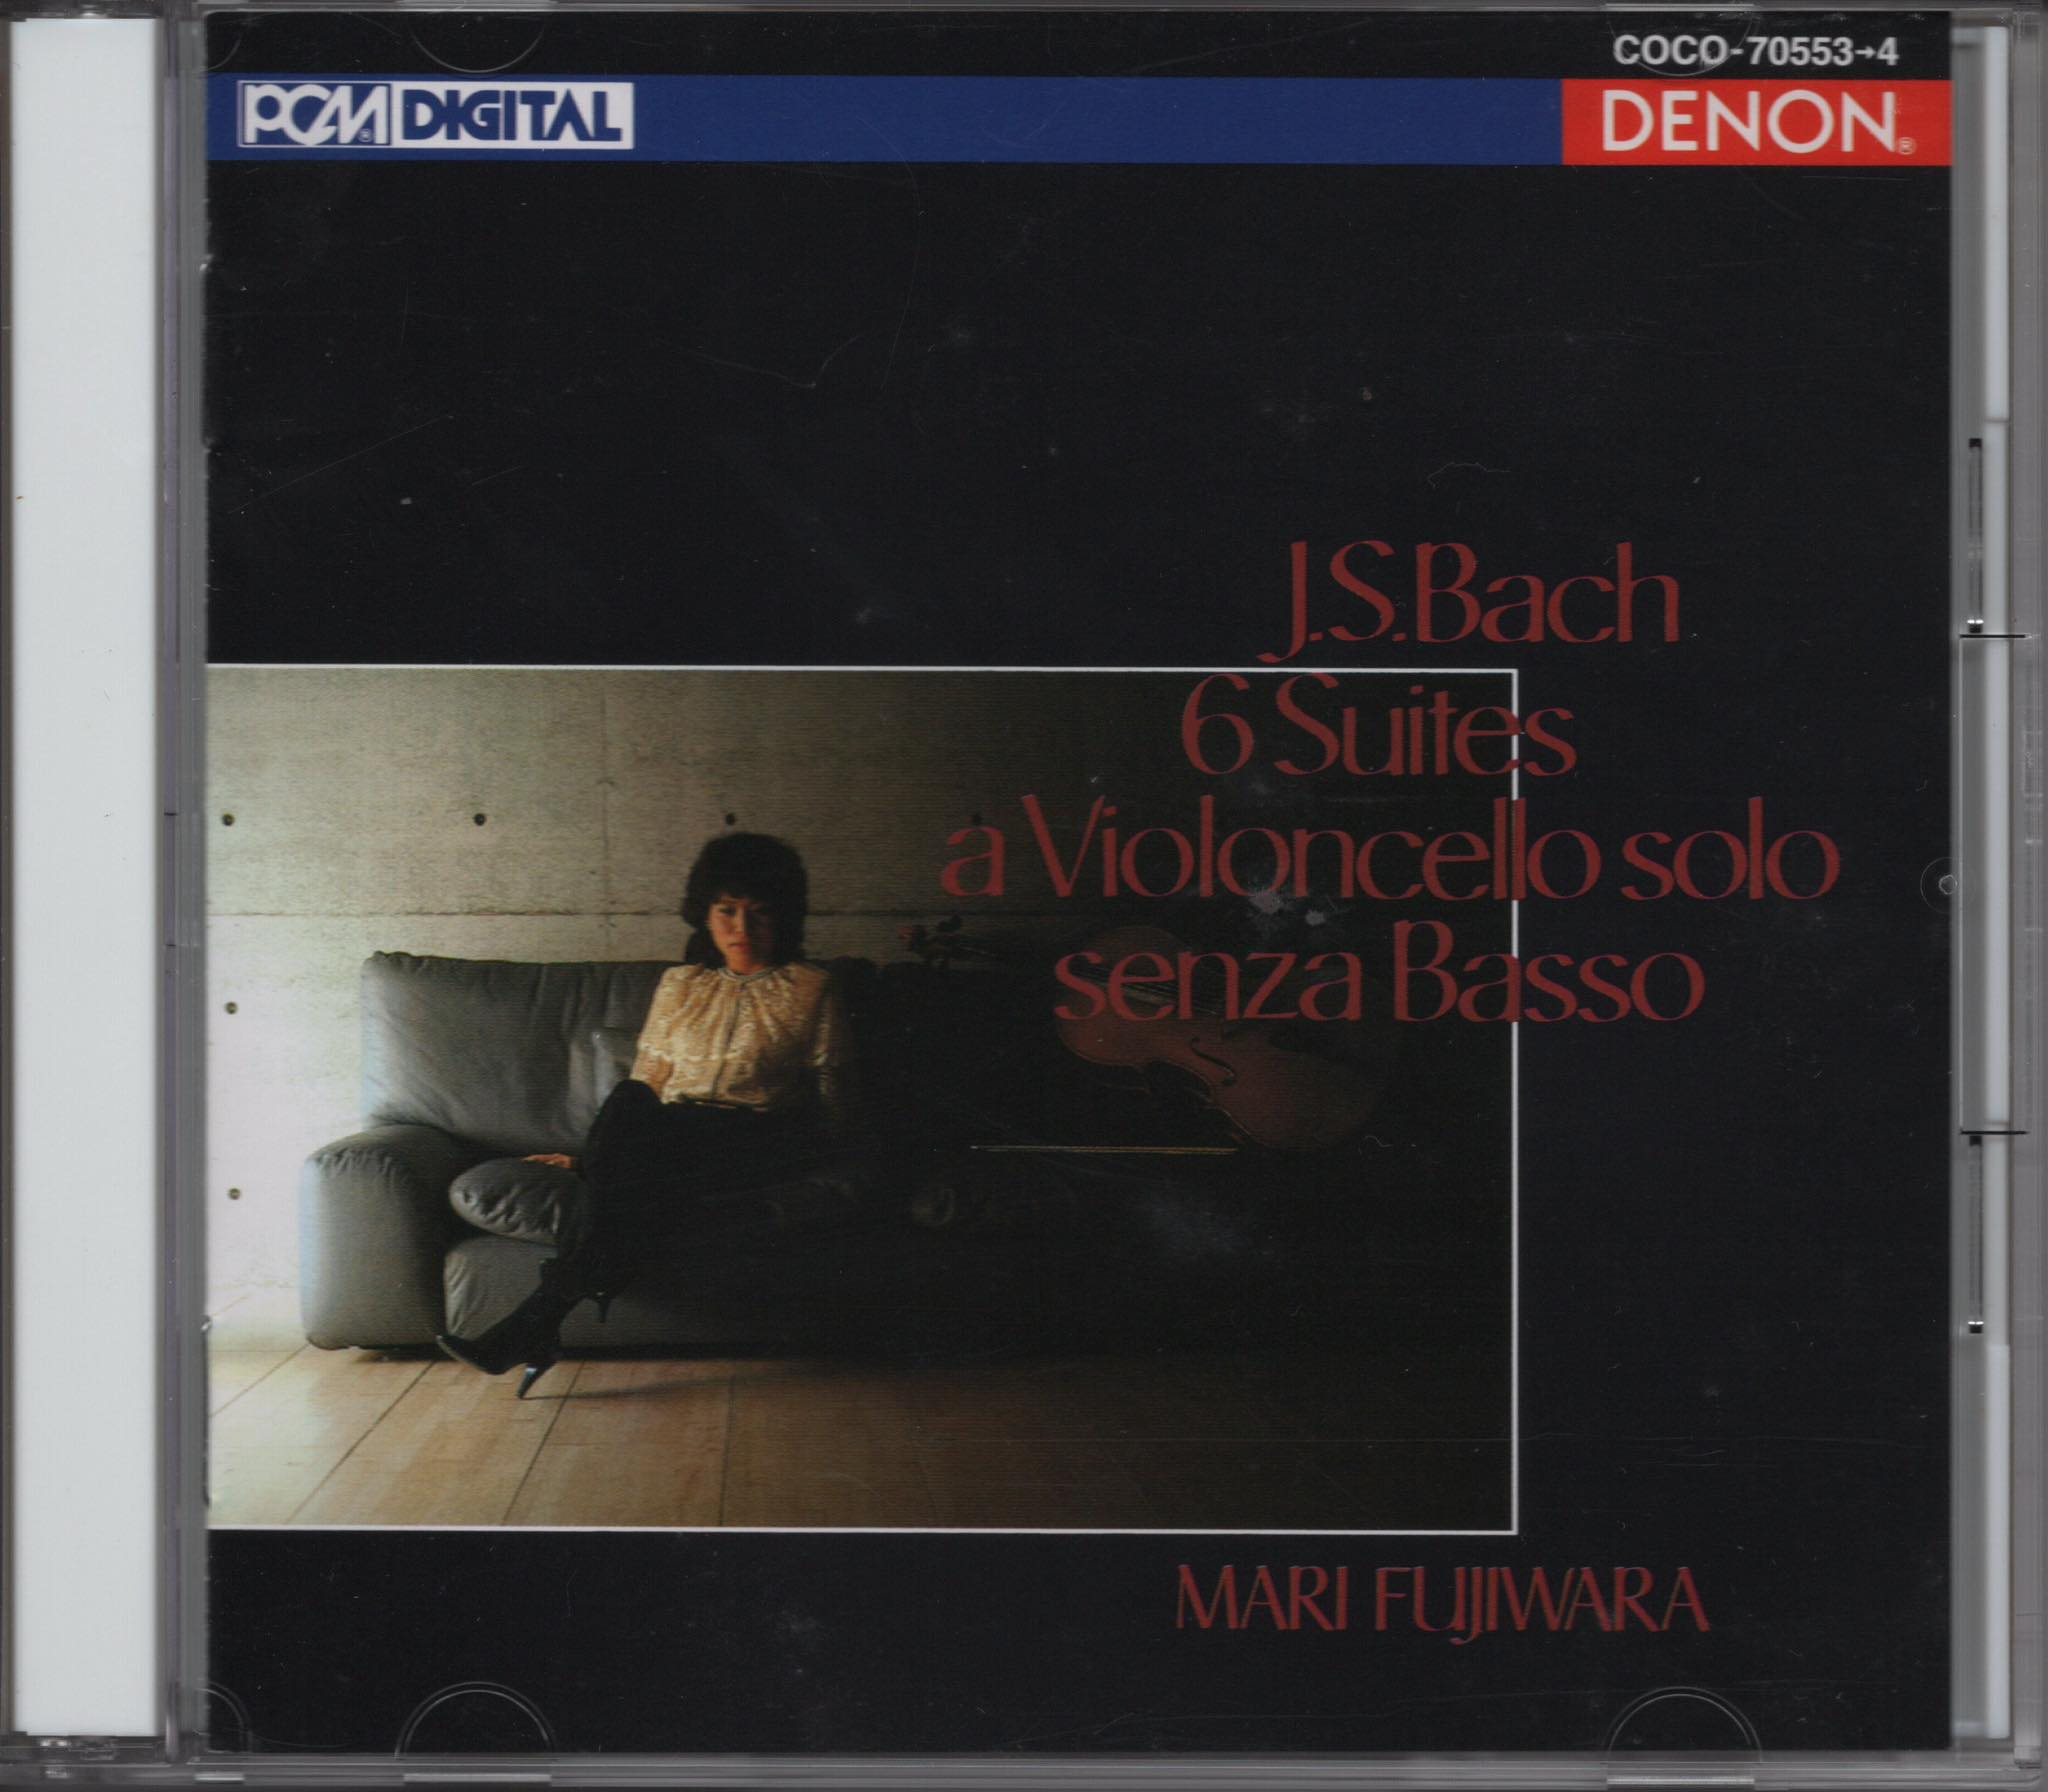
\includegraphics[width=\linewidth]{pictures/2026/03/20260317_052218_001.jpg}
\end{minipage}
\hfill
\begin{minipage}{0.48\linewidth}
\centering
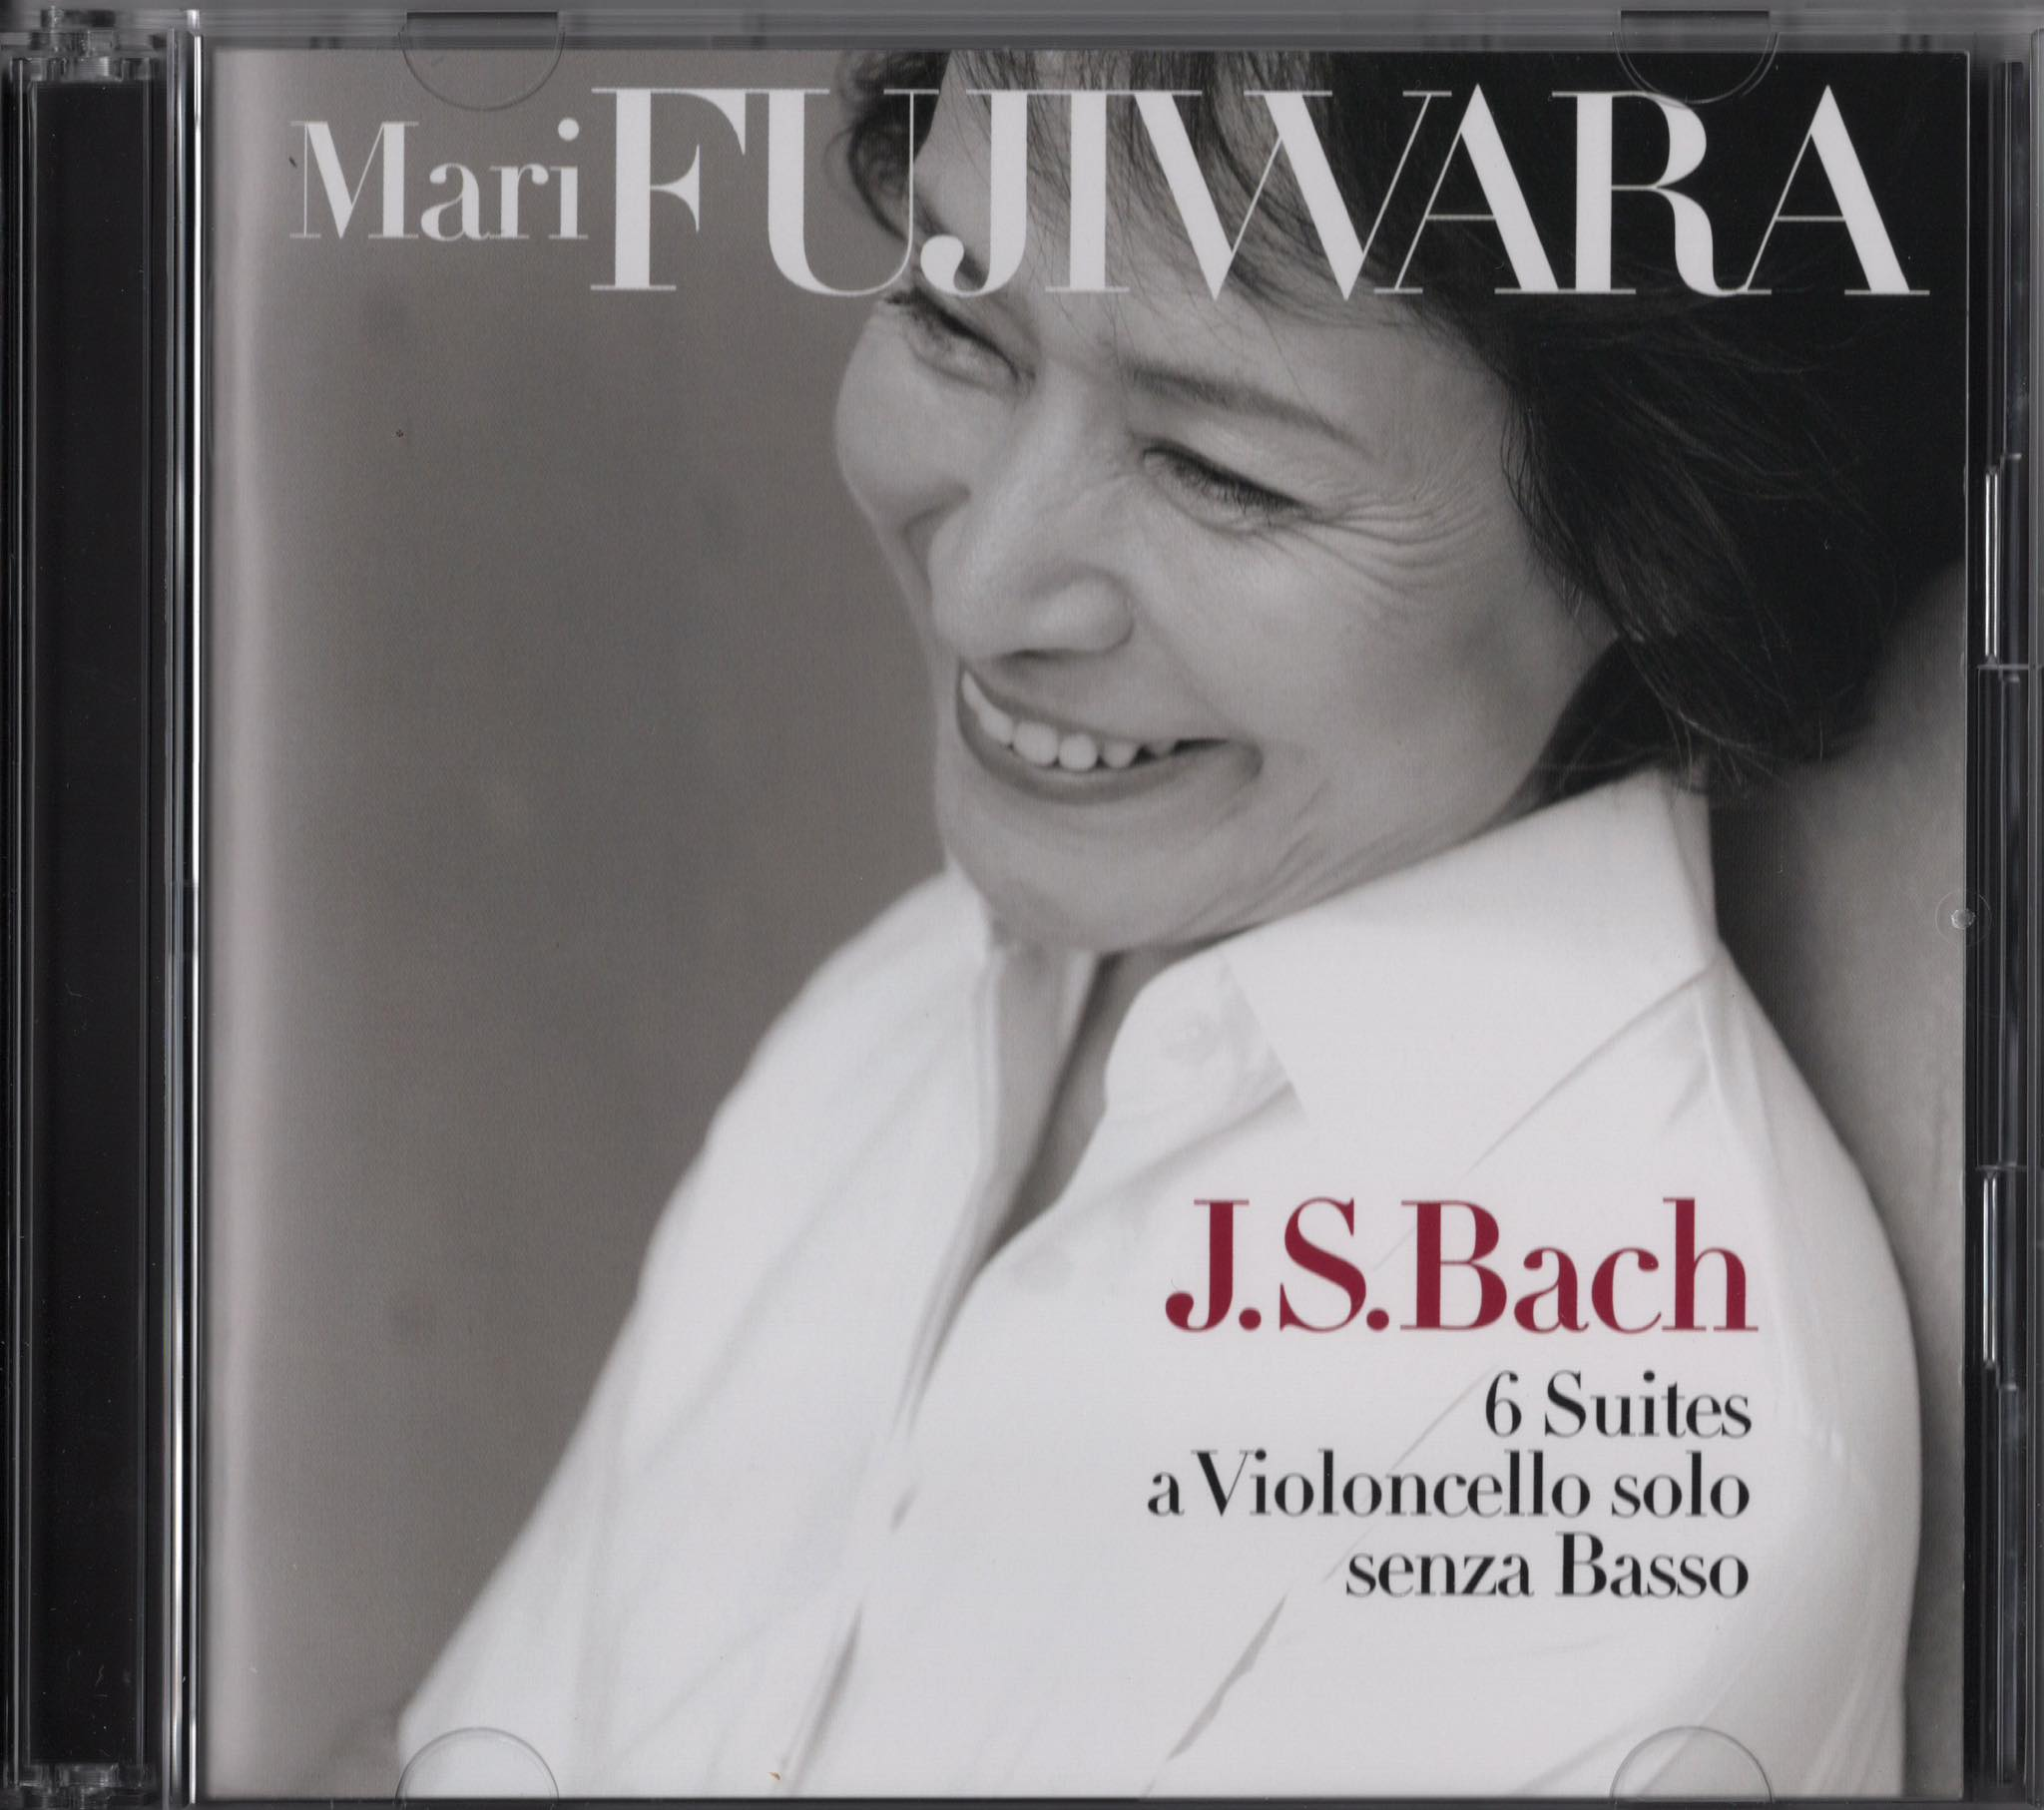
\includegraphics[width=\linewidth]{pictures/2026/03/20260317_052218_002.jpg}
\end{minipage}
\end{center}

\subsection*{2026年03月18日 20:09}
\addcontentsline{toc}{subsection}{2026年03月18日 20:09}

NHKはありがたい！

私の様な素人にも最先端の研究成果を分かりやすく教えてくれる。

とても面白かった。きょう3月18日に「普通の」BSで放送してくれました。（4Kの設備は持っていませんから）


\url{https://www.web.nhk/tv/an/frontiers/pl/series-tep-PM34JL2L14/ep/K6VLYQ6YX2}




これを見ていて、研究でも「多様性」が重要なんだなと思いました。天文学者、素粒子物理学者、宇宙物理学者、などなど、それぞれの視点で見た時に、一つに視点だけでは思いつかない様な、新たな知見に到達出来る可能性が出てくるんだと思いました。（「選択と集中」などといった、多様性を潰す様な政策は残念だという気がします）


再放送は↓


NHK BS

3月24日(火)午前9:00〜午前10:00


===

以下の記事の続きです

\url{https://m.facebook.com/story.php?story_fbid=25150691187921705&id=100002225117991}



\paragraph{写真}
\begin{center}
\begin{minipage}{0.48\linewidth}
\centering
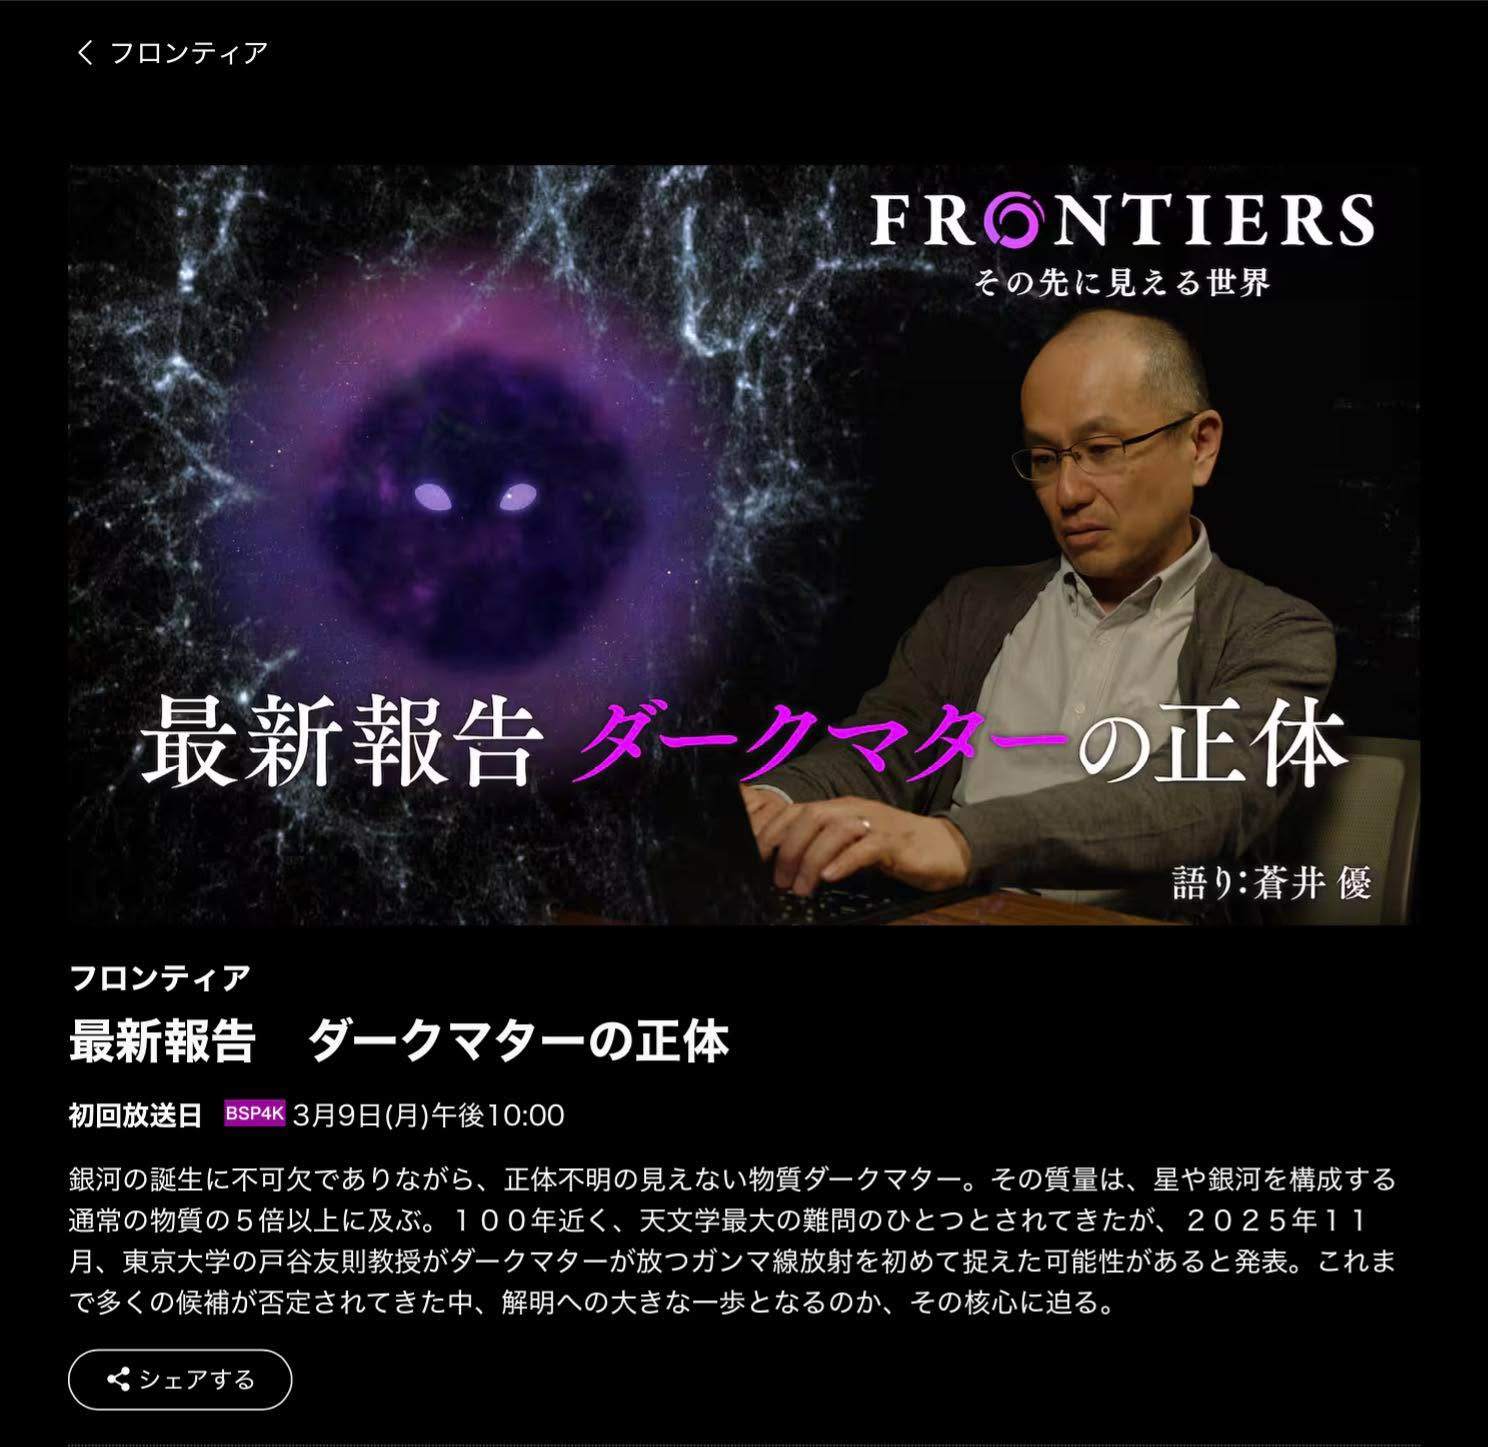
\includegraphics[width=\linewidth]{pictures/2026/03/20260318_200932_001.jpg}
\end{minipage}
\end{center}

\subsection*{2026年03月19日 08:54}
\addcontentsline{toc}{subsection}{2026年03月19日 08:54}

これは良い！作ってみたいものです

\url{https://youtu.be/rA0DlM5BObM}

\begin{center}
\href{https://youtu.be/rA0DlM5BObM}{
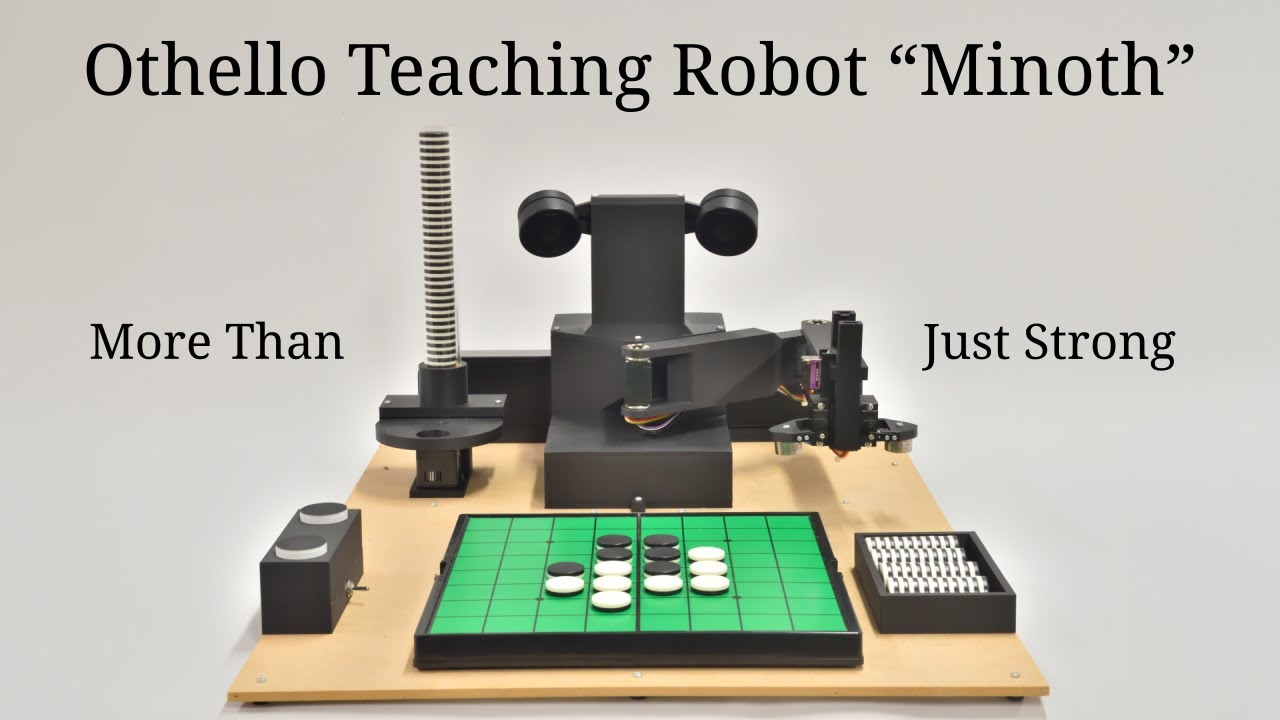
\includegraphics[width=0.48\linewidth]{pictures/youtube/2026/03/20260319_085404_youtube_001_rA0DlM5BObM.jpg}
}
\end{center}



\url{https://youtu.be/Ok0Ple36Ebs}

\begin{center}
\href{https://youtu.be/Ok0Ple36Ebs}{
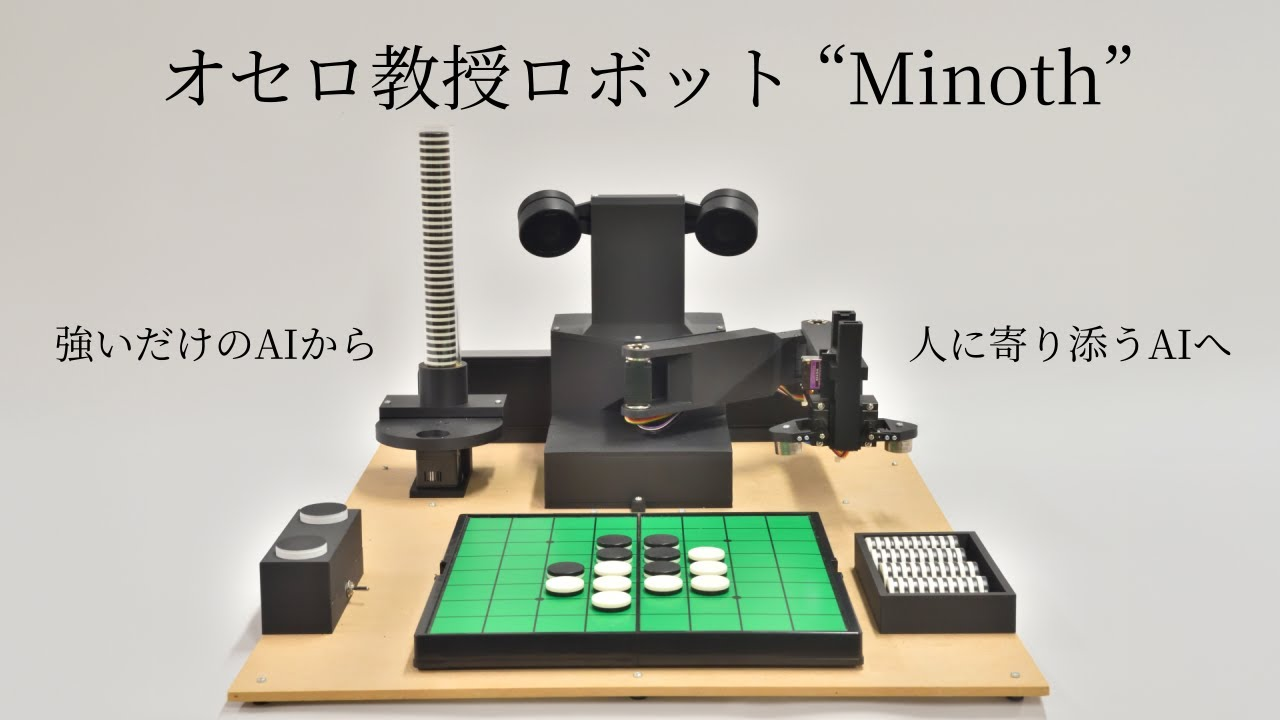
\includegraphics[width=0.48\linewidth]{pictures/youtube/2026/03/20260319_085404_youtube_002_Ok0Ple36Ebs.jpg}
}
\end{center}



\url{https://youtu.be/4RupB59MNIQ}

\begin{center}
\href{https://youtu.be/4RupB59MNIQ}{
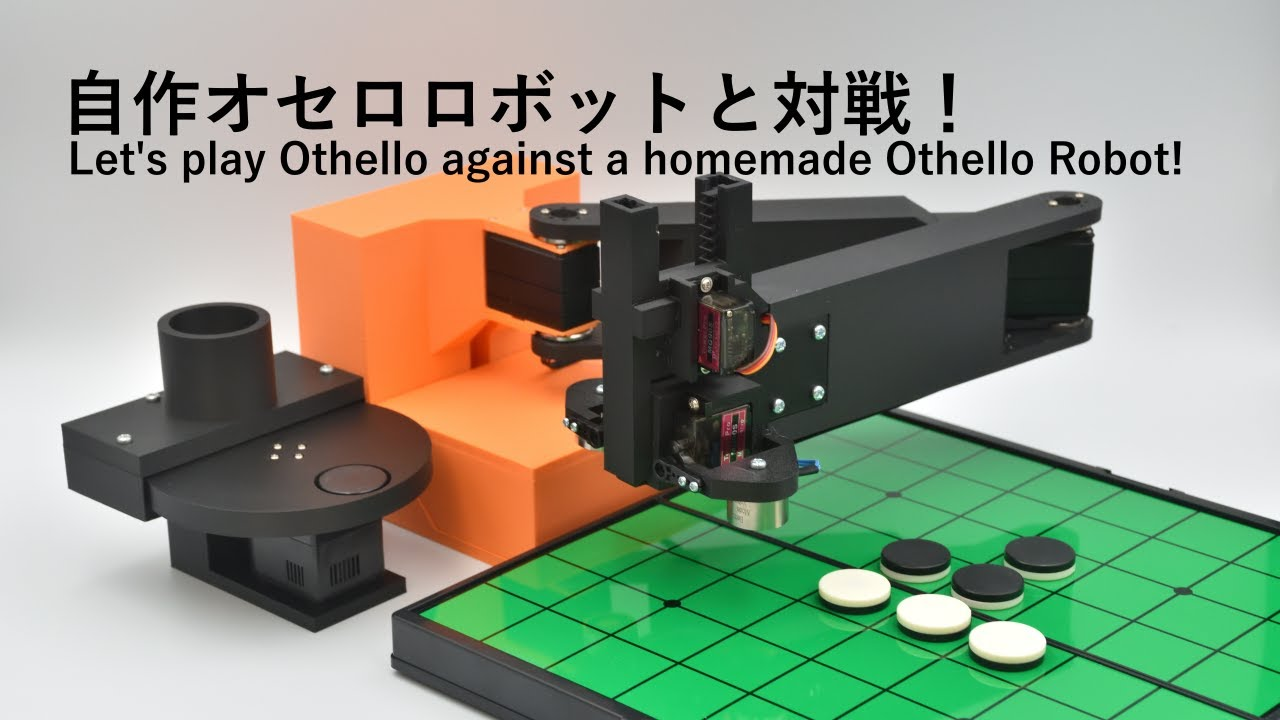
\includegraphics[width=0.48\linewidth]{pictures/youtube/2026/03/20260319_085404_youtube_003_4RupB59MNIQ.jpg}
}
\end{center}



\url{https://youtu.be/bV2cLeHRmJw}

\begin{center}
\href{https://youtu.be/bV2cLeHRmJw}{
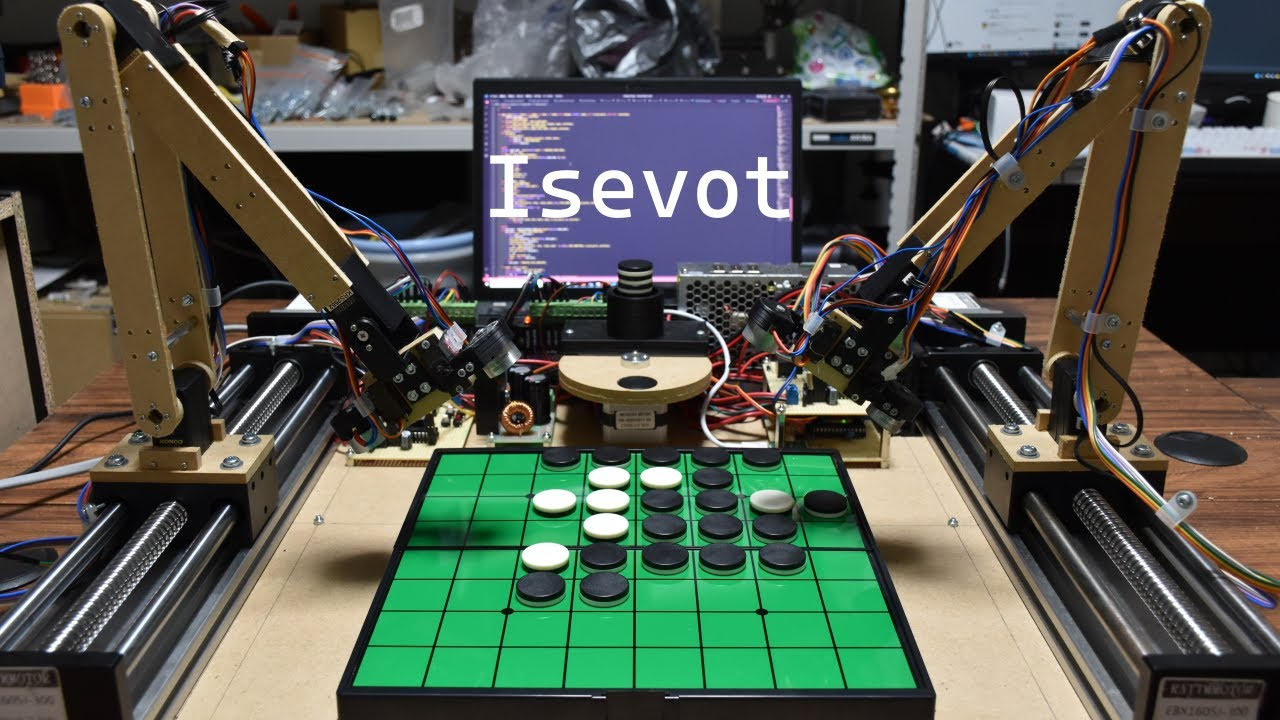
\includegraphics[width=0.48\linewidth]{pictures/youtube/2026/03/20260319_085404_youtube_004_bV2cLeHRmJw.jpg}
}
\end{center}




ゲームの頭脳部分は（近年のAIではないが、αβカットの戦略まで）Okなので、とりあえず作るのはメカ部とその制御だけだが、、、

\url{https://m.facebook.com/story.php?story_fbid=6639337476150357&id=100002225117991}




石を裏返すメカが面白い！（電磁石？）アームの先端はサーボモータ３個か？

ロボットのアームを指定した座標位置へ動かすために、どのモーターをどれだけ動かすのか？力尽くの計算で解決できる？ステッピングモーターは何個？２個だけかな？そう言えば石を供給している台も回っている様だ

一方でチョット気になるのは、、、どうも目を持っているみたいだな（どこに石が置かれているかの画像認識が必要なのか←これは、ちょっと困った）画像認識は以前Cloudサービスとの連携で比較的上手くいくのがあったけど、出来ればローカルに実現したいものです


これ↓（Raspberry pi用AI HAT）で何とかならんかな？

\url{https://www.facebook.com/100068543340423/posts/1210076401287127/}




これ↓も面白いことになっている

\url{https://fb.watch/GUNEG-Qy6U/}



\paragraph{写真}
\begin{center}
\begin{minipage}{0.48\linewidth}
\centering
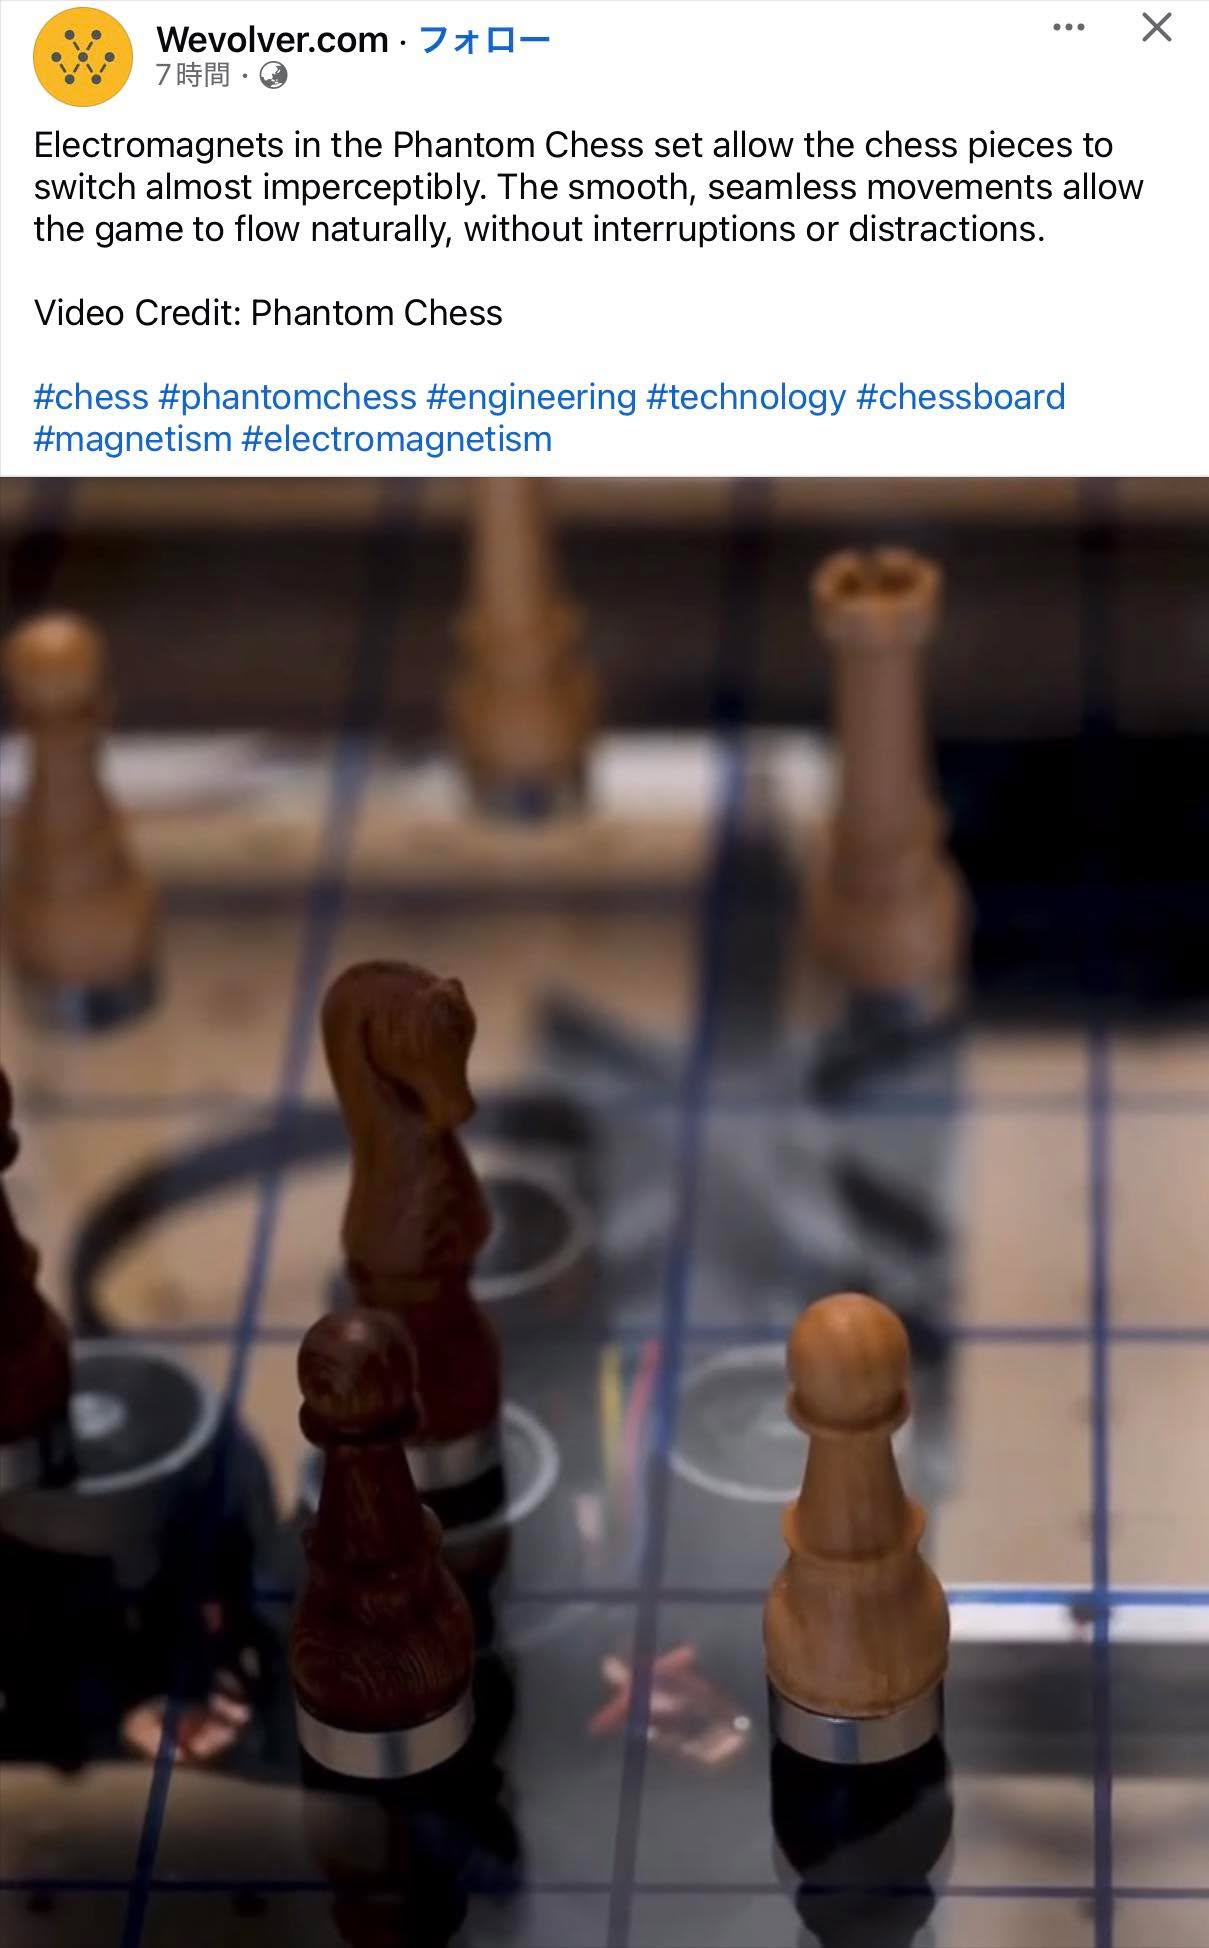
\includegraphics[width=\linewidth]{pictures/2026/03/20260319_085404_001.jpg}
\end{minipage}
\hfill
\begin{minipage}{0.48\linewidth}
\centering
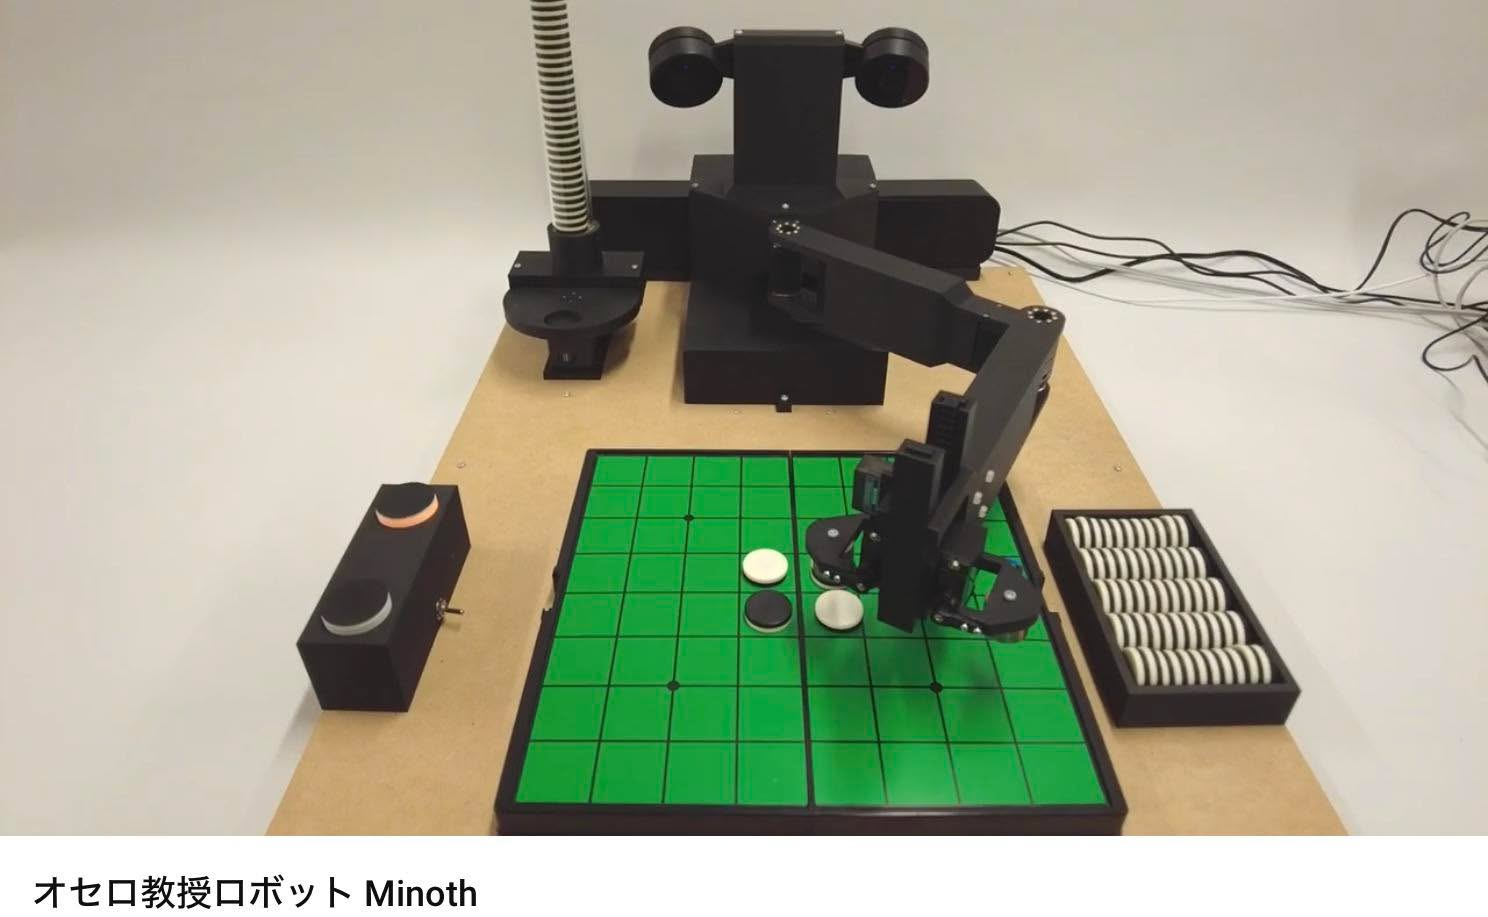
\includegraphics[width=\linewidth]{pictures/2026/03/20260319_085404_002.jpg}
\end{minipage}
\end{center}

\subsection*{2026年03月19日 11:21}
\addcontentsline{toc}{subsection}{2026年03月19日 11:21}

作ってみたいもの（3Dプリンタがあるので、どんな形でも自由だ）


(１)リコーダー

\url{https://www.facebook.com/100002225117991/posts/25313842881606534/}




(２)オセロ

\url{https://www.facebook.com/100002225117991/posts/26116390278018453/}




(３)ルービックキューブ

\url{https://www.facebook.com/100002225117991/posts/26117470181243796/}




(４)オルガン

\url{https://www.facebook.com/100002225117991/posts/26117501274574020/}




(５)村田製作くん

\url{https://m.facebook.com/story.php?story_fbid=8274693622614726&id=100002225117991}



\subsection*{2026年03月19日 11:37}
\addcontentsline{toc}{subsection}{2026年03月19日 11:37}

製作できないかと前から思っていた


\url{https://youtu.be/9rOV35XQlQI}

\begin{center}
\href{https://youtu.be/9rOV35XQlQI}{
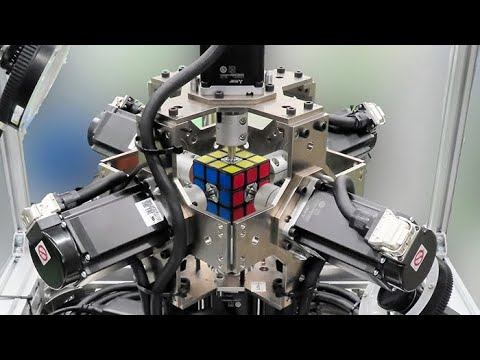
\includegraphics[width=0.48\linewidth]{pictures/youtube/2026/03/20260319_113742_youtube_001_9rOV35XQlQI.jpg}
}
\end{center}




スピードは要らないので、ゆっくり動作が見える様にしたい

筐体は3Dプリンタで作れば十分でしょう

ステッピングモータは幾つ必要？６個？（小さい＝安いのでいいよね）

ステッピングモータの制御などは（得意の）Raspberry Pi（とPython）でいくことにしよう


でも実は最も問題なのは、そもそも頭脳部分（解法）が分かっていない事です

\url{https://www.facebook.com/100002225117991/posts/26210254245298722/}



\subsection*{2026年03月19日 11:42}
\addcontentsline{toc}{subsection}{2026年03月19日 11:42}

これは作るの難しいのかな？

ごちゃごちゃしていて、少なくともチョット面倒そうには見えます（仕組みは思い当たるのですが）

\url{https://youtu.be/cG3VHvKCDzQ}

\begin{center}
\href{https://youtu.be/cG3VHvKCDzQ}{
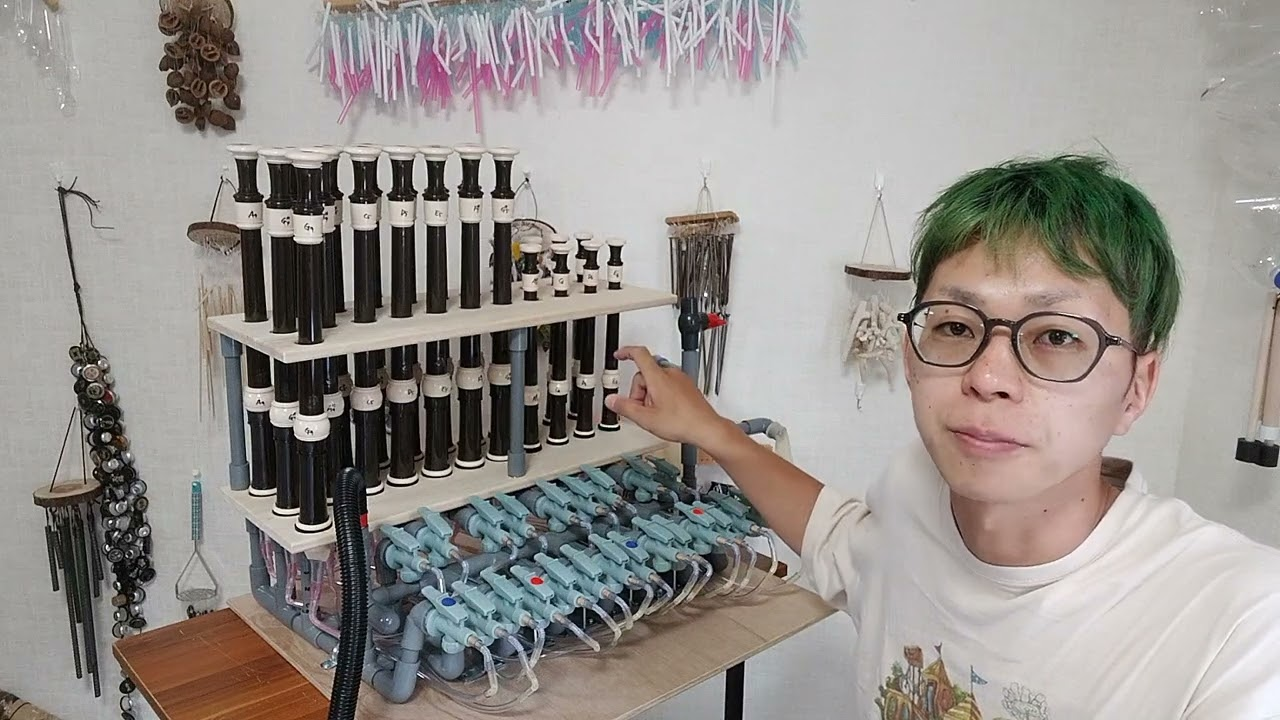
\includegraphics[width=0.48\linewidth]{pictures/youtube/2026/03/20260319_114222_youtube_001_cG3VHvKCDzQ.jpg}
}
\end{center}



\subsection*{2026年03月20日 09:14}
\addcontentsline{toc}{subsection}{2026年03月20日 09:14}

相手を本当に知るためには、フル・スィング（全力）で議論する事だ！


\url{https://www.facebook.com/photo.php?fbid=122233486694290594&set=a.122143182782290594&type=3}




私は「その通りだね」と思ってしまったけど、コメントを見ると必ずしも好意的には捉えられていない様です。楽観的だとか、そんな必要無い、という様な見方が散見され、ちょっと意外でした。（近年のイスラエルの軍事行動があってのコメントなのかもしれません）

\subsection*{2026年03月21日 09:21}
\addcontentsline{toc}{subsection}{2026年03月21日 09:21}

誕生日をお祝いする人がいるのか

（没後なん年というのはありそうですが）


\url{https://m.facebook.com/groups/189030912198717/permalink/1555229635578831/}




Wikiぺディア周辺で調べた補足説明を（勝手ながら）加えさせて頂きながら、気付いた点を（何となく）書いていく事にすると、


(１)アイゼナハとチューリンゲン

バッハが生まれたのは、（現在の）チューリンゲン州（Freistaat Thüringen）にあるアイゼナハ（Eisenach）


(２)誕生日の記述がユリウス暦で3月21日

ユリウス暦は紀元前45年にローマ帝国のユリウス（カエサル）が定めた暦で、16世紀末には10日間ほどの実際とのズレが生じていた。1582年にローマ教皇のグレゴリオさんが修正してグレゴリオ暦を始めた。

バッハが生まれたのは1685年との事なので、世界史的にはグレゴリオ暦が始まって凡そ100年を経ている事になるが、当時のチューリンゲン地方周辺では未だユリウス暦が使われていたらしく、誕生日の記述はユリウス暦によるものだった。グレゴリオ暦がユリウス暦から10日程ズレている事を考慮すると、（現在の3月31日を、当時は3月21日と言っていた＝＞現在の3月21日は、当時であれば3月11日と言っていた）バッハが誕生したその日は、実は現在の3月31日だったという事になるのかな。


(３)因みに命日は

亡くなったのは（現在の）ザクセン州にあるラプツイッヒで、ユリウス暦による1750年７月17日。これがグレゴリオ暦では（約10日程ずらして）7月28日。これを命日とするのが一般的との事です（バッハが生まれる100年前にはグレゴリオ暦になっているというのに、バッハがいた周辺地域では少なくとも亡くなる年までユリウス暦が使われていたと言う事ですか）


(４)チューリンゲン州（地方）とザクセン州（地方）

現在は「州」で区切られているが、当時はひとつの州ではなく、細かく分かれた諸侯領の集合体だった様なので、「州」と言うより「地方」と言ったほうが良いのかもしれない


(５)バッハ像の正面に刻まれている名前を見ると頭3文字で略されている（JOH.SEB.BACH ← Johann Sebastian Bach）のが分かる


(６) JOH.SEB.BACHのJ が I になっている事について

ラテン語にJの文字が無いので I で代用された（ラテン語には U も無いので V で代用される←チェンバロにMVSICと書かれていた記憶がある）ただ、バッハ像の文字に「ラテン語で」文字が刻まれる必然性は何なんだろうか？


ChatGPTによるお答え

====

このラテン語表記には

• 学問・教養の国際語としての伝統

• 記念碑にふさわしい格式・普遍性の強調

• 18世紀の実際の命名慣習の反映

という三つの理由が重なっており、単なる装飾ではなく「歴史的に自然な選択」だと言えます

====

\subsection*{2026年03月22日 15:01}
\addcontentsline{toc}{subsection}{2026年03月22日 15:01}

\paragraph{リンク}
\url{https://maps.app.goo.gl/xtjHUAUSZZeV7LfQ8?g_st=ic}

\subsection*{2026年03月24日 11:00}
\addcontentsline{toc}{subsection}{2026年03月24日 11:00}

（ネタばれあり←再再放送終わってるからいいかな？）

3月24日NHK BS Frontiers「ダークマターの正体」の再放送を（再度）見た


(１)ウェラ・ルービン（天文学者）1970年「アンドロメダ銀河の回転」

⚪︎星のスペクトルを観察して星の移動速度を推測った所、銀河の中心の星の速度と銀河周辺の星の速度が変わらなかった←何か重いものが無いと周辺の星は銀河から離脱するはず

⚪︎その後100を越える銀河でも同様の観測をして同じ様な結果を得た→見えていない何かが有るらしいとなった


(２)重力レンズの効果を観察→暗黒物質の3次元分布が得られた


(３)宇宙の始まりで暗黒物質が無かったら、星も銀河も生成されない事がコンピュータ シミュレーションによって示された（暗黒物質は、そもそも必要なものだった）


(４)白色矮星などの暗くて重い星が暗黒物質の候補とも考えられたが、重さを合計しても暗黒物質に及ばない（暗い星は暗黒物質を構成していない）


(５)ニュートリノに重さがあると分かった（カミオカンデ）が、暗黒物質には到底足りない（暗黒物質はニュートリノではない）


(６)未知の（素）粒子Winp（陽子の100倍の重さ）が暗黒物質である可能性が予想されているが、そもそも見つかっていない←現段階では観測データ不足


(７)NASAの観測衛星（フェルミ・ガンマ線宇宙望遠鏡）によるガンマ線マップのデータ

⚪︎Winpの対消滅（ついしょうめつ）に伴ってガンマ線が放出される

⚪︎フェルミ望遠鏡による15年間のガンマ線観測データから、理由が判明しているガンマ線データを丁寧に取り除いていった所、残ったガンマ線データはWinpの対消滅によって生じたもの（かもしれない）

⚪︎その残ったガンマ線が銀河の中心から球対称状に分布しており、銀河の中心ほど密度が濃い（←中心ほど暗黒物質が多い）ことが可視化された

⚪︎戸谷氏の今回の論文（注目された）はこれ↑（←ダークマターが「見えた」のではないか？という事）


(８)宇宙の初期からWinpの対消滅（によるガンマ線生成）が起きていたなら、現在までに（対消滅してガンマ線を出す）Winpが残っていないのでは？という疑問に対して、現在までWinpの対消滅が発生している理由を、村山氏（素粒子物理学）が直後に論文で説明して戸谷氏を後押し


===

以下の記事の続きです

\url{https://m.facebook.com/story.php?story_fbid=26111141618543319&id=100002225117991}



\subsection*{2026年03月24日 21:01}
\addcontentsline{toc}{subsection}{2026年03月24日 21:01}

火星の日没は青い（赤くない）のか


\url{https://x.com/naturesciencea1/status/2036200200952496403}



\paragraph{リンク}
\url{https://x.com/naturesciencea1/status/2036200200952496403?s=61&t=5VtsOkpki6juEjPXsBq8hg}

\subsection*{2026年03月27日 08:25}
\addcontentsline{toc}{subsection}{2026年03月27日 08:25}

応援中: 山下 愛陽 ― トップファンに認定されました！🎉


\url{https://www.facebook.com/100002225117991/posts/25501583942832426/}




（その後）

おっと、コレはOnline streaming付きだ！（4月8日19時〜）

Liveの席は完売ですね

\url{https://m.facebook.com/story.php?story_fbid=4409307712681128&id=100008058284613}




Online streamingのticket購入はここ（¥1500）

\url{https://www.harusailive.jp/offer/OF743G1BZTQ8}



（マンションのネット回線環境、今どき光じゃないから、不安定で遅いからなぁ😢）

\paragraph{写真}
\begin{center}
\begin{minipage}{0.48\linewidth}
\centering
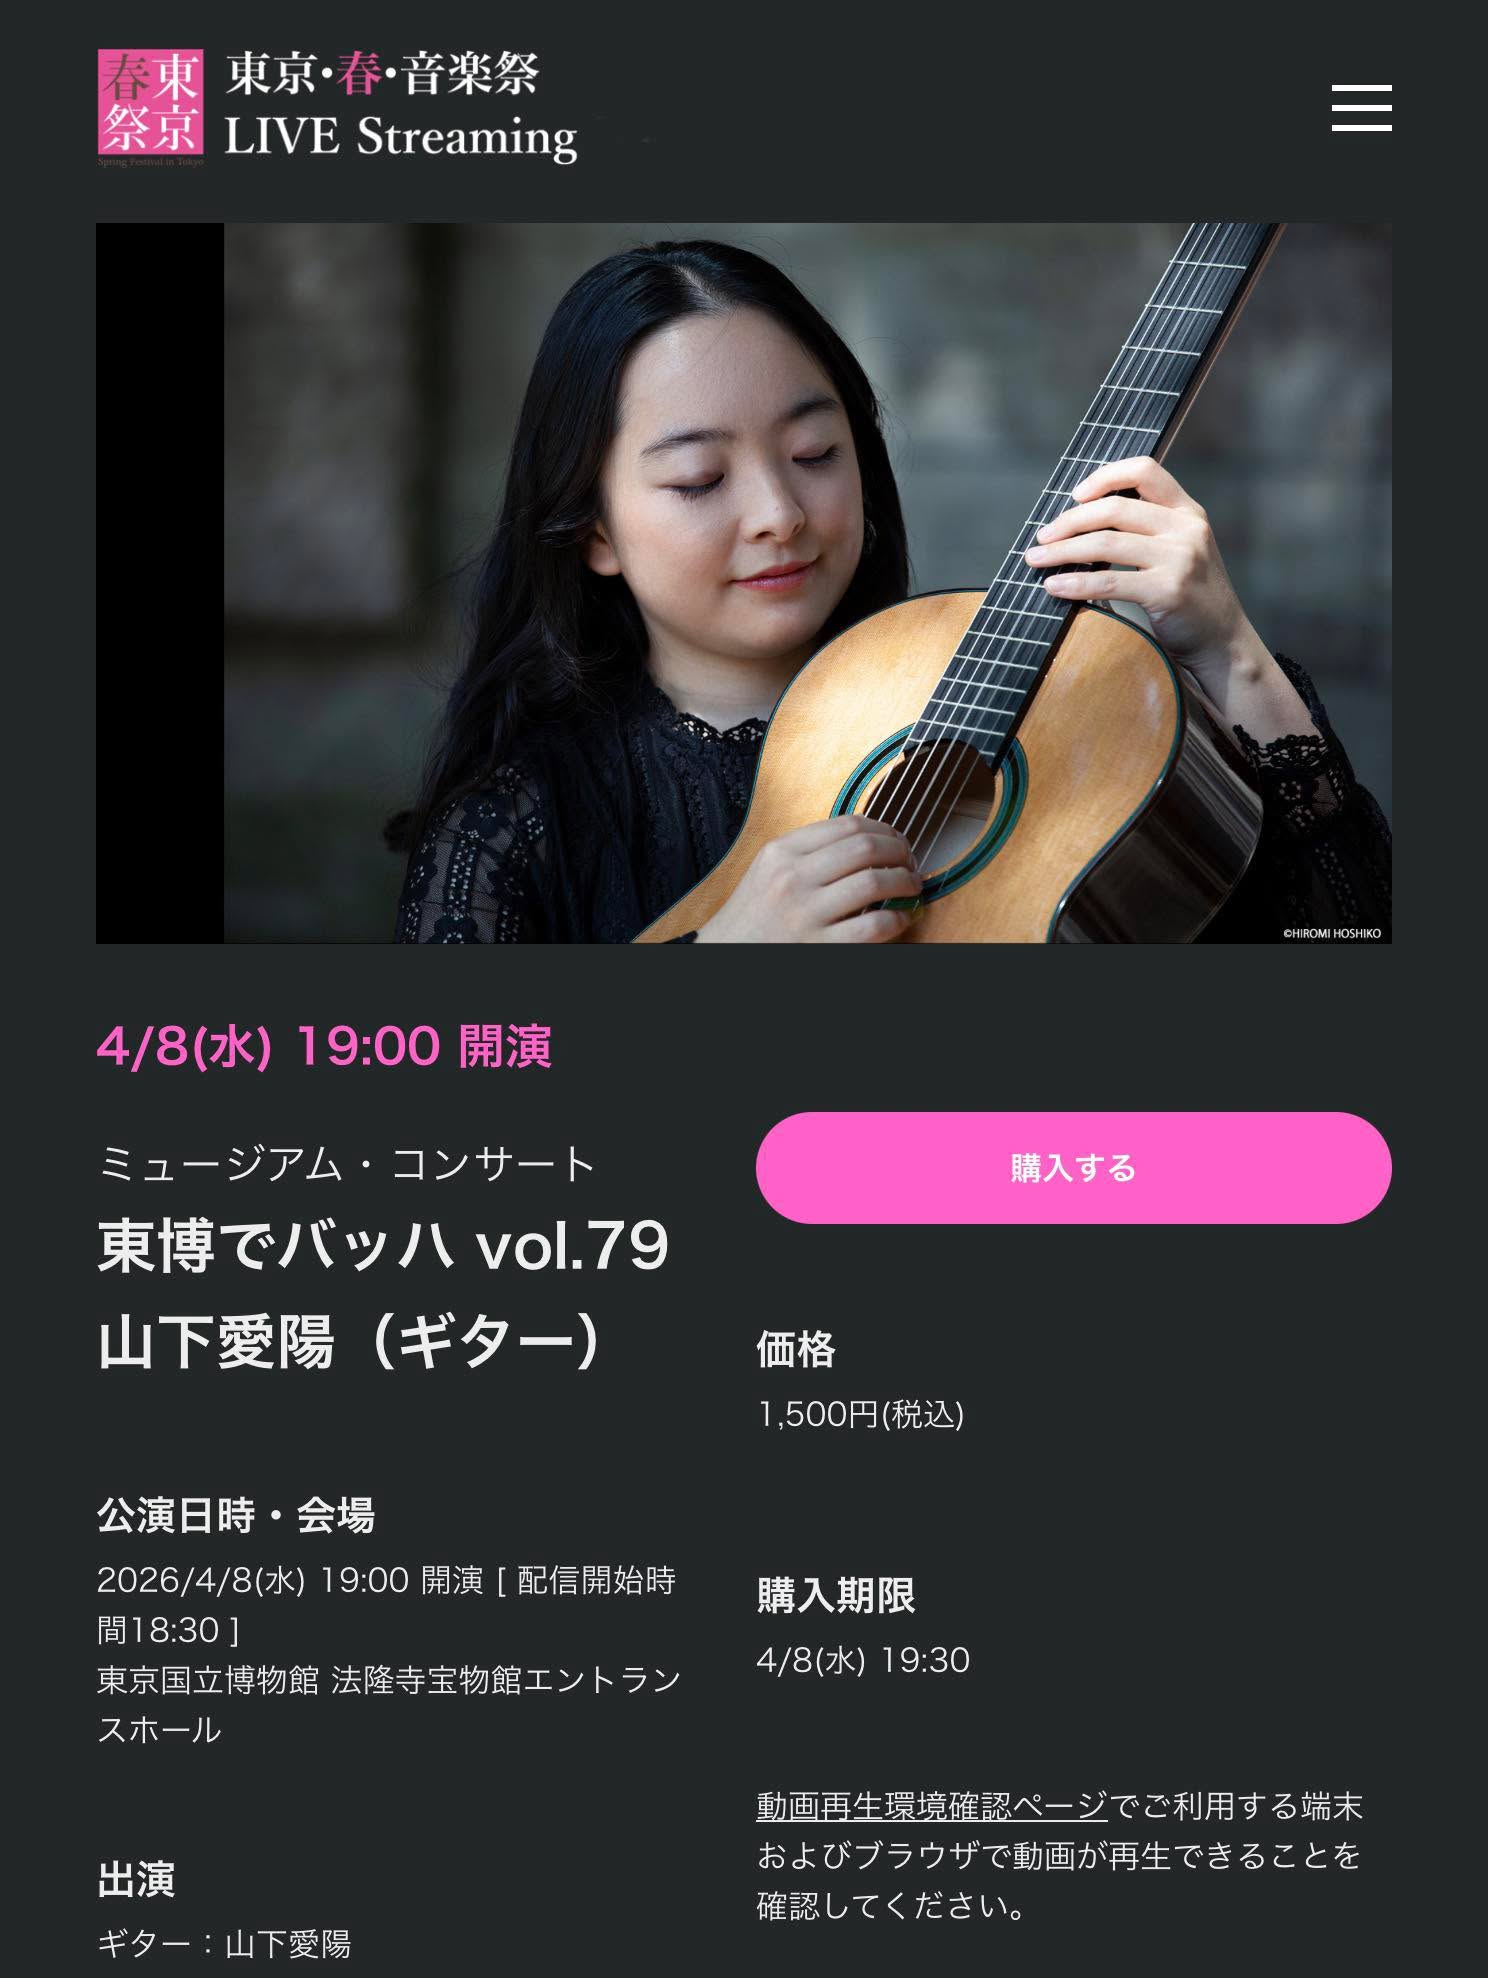
\includegraphics[width=\linewidth]{pictures/2026/03/20260327_082522_001.jpg}
\end{minipage}
\end{center}

\subsection*{2026年03月27日 19:24}
\addcontentsline{toc}{subsection}{2026年03月27日 19:24}

\paragraph{リンク}
\url{https://x.com/rainmaker1973/status/2037215422731145440}

\subsection*{2026年03月28日 01:34}
\addcontentsline{toc}{subsection}{2026年03月28日 01:34}

ルービックキューブに真面目に取り組んでみようと思いはじめた


解法より先に、ルービックキューブの「状態」や「操作」を正確に表現(記述）する手立てが必要なのだ（そのために数学、ここでは群論が必要になる）という気になってきた


そう言えば、ルービックキューブが流行るより前に、古くから「15パズル」はポピュラーだった（どちらも「置換という操作」によるパズルだったのか）


島内剛一氏によるルービックキューブに関する著作は、確かルービックキューブが最初に流行り始めた頃からあった様に記憶しているが、今ではもう売られていないみたいです（古本なら手に入るか）


解法だけが目的なら（群論を知らなくても）、公開されている通りに（盲目的に）操作すれば解くことができる事は出来るのだが、、、


島内氏の著書「ルービックキューブと数学パズル」では、前半で解法を色々紹介した後、後半で数学の解説がなされている（後半は必要に応じて参照下さいという感じか？）でも、著者は数学者でいらしたので本当は後半にこの本の主眼があるのでしょうけど

もう一方の「群論の味わい」では、数学の解説が殆どを占めており、最後の方で（前半で紹介された数学上の言葉、記述法を使って）解法についても触れられている（ただ前半の演習や例題などで、ルービックキューブは数学を説明する具体的な演習対象として扱われている）


===

以下↓の記事の続きです

\url{https://www.facebook.com/100002225117991/posts/26117470181243796/}



\paragraph{写真}
\begin{center}
\begin{minipage}{0.48\linewidth}
\centering
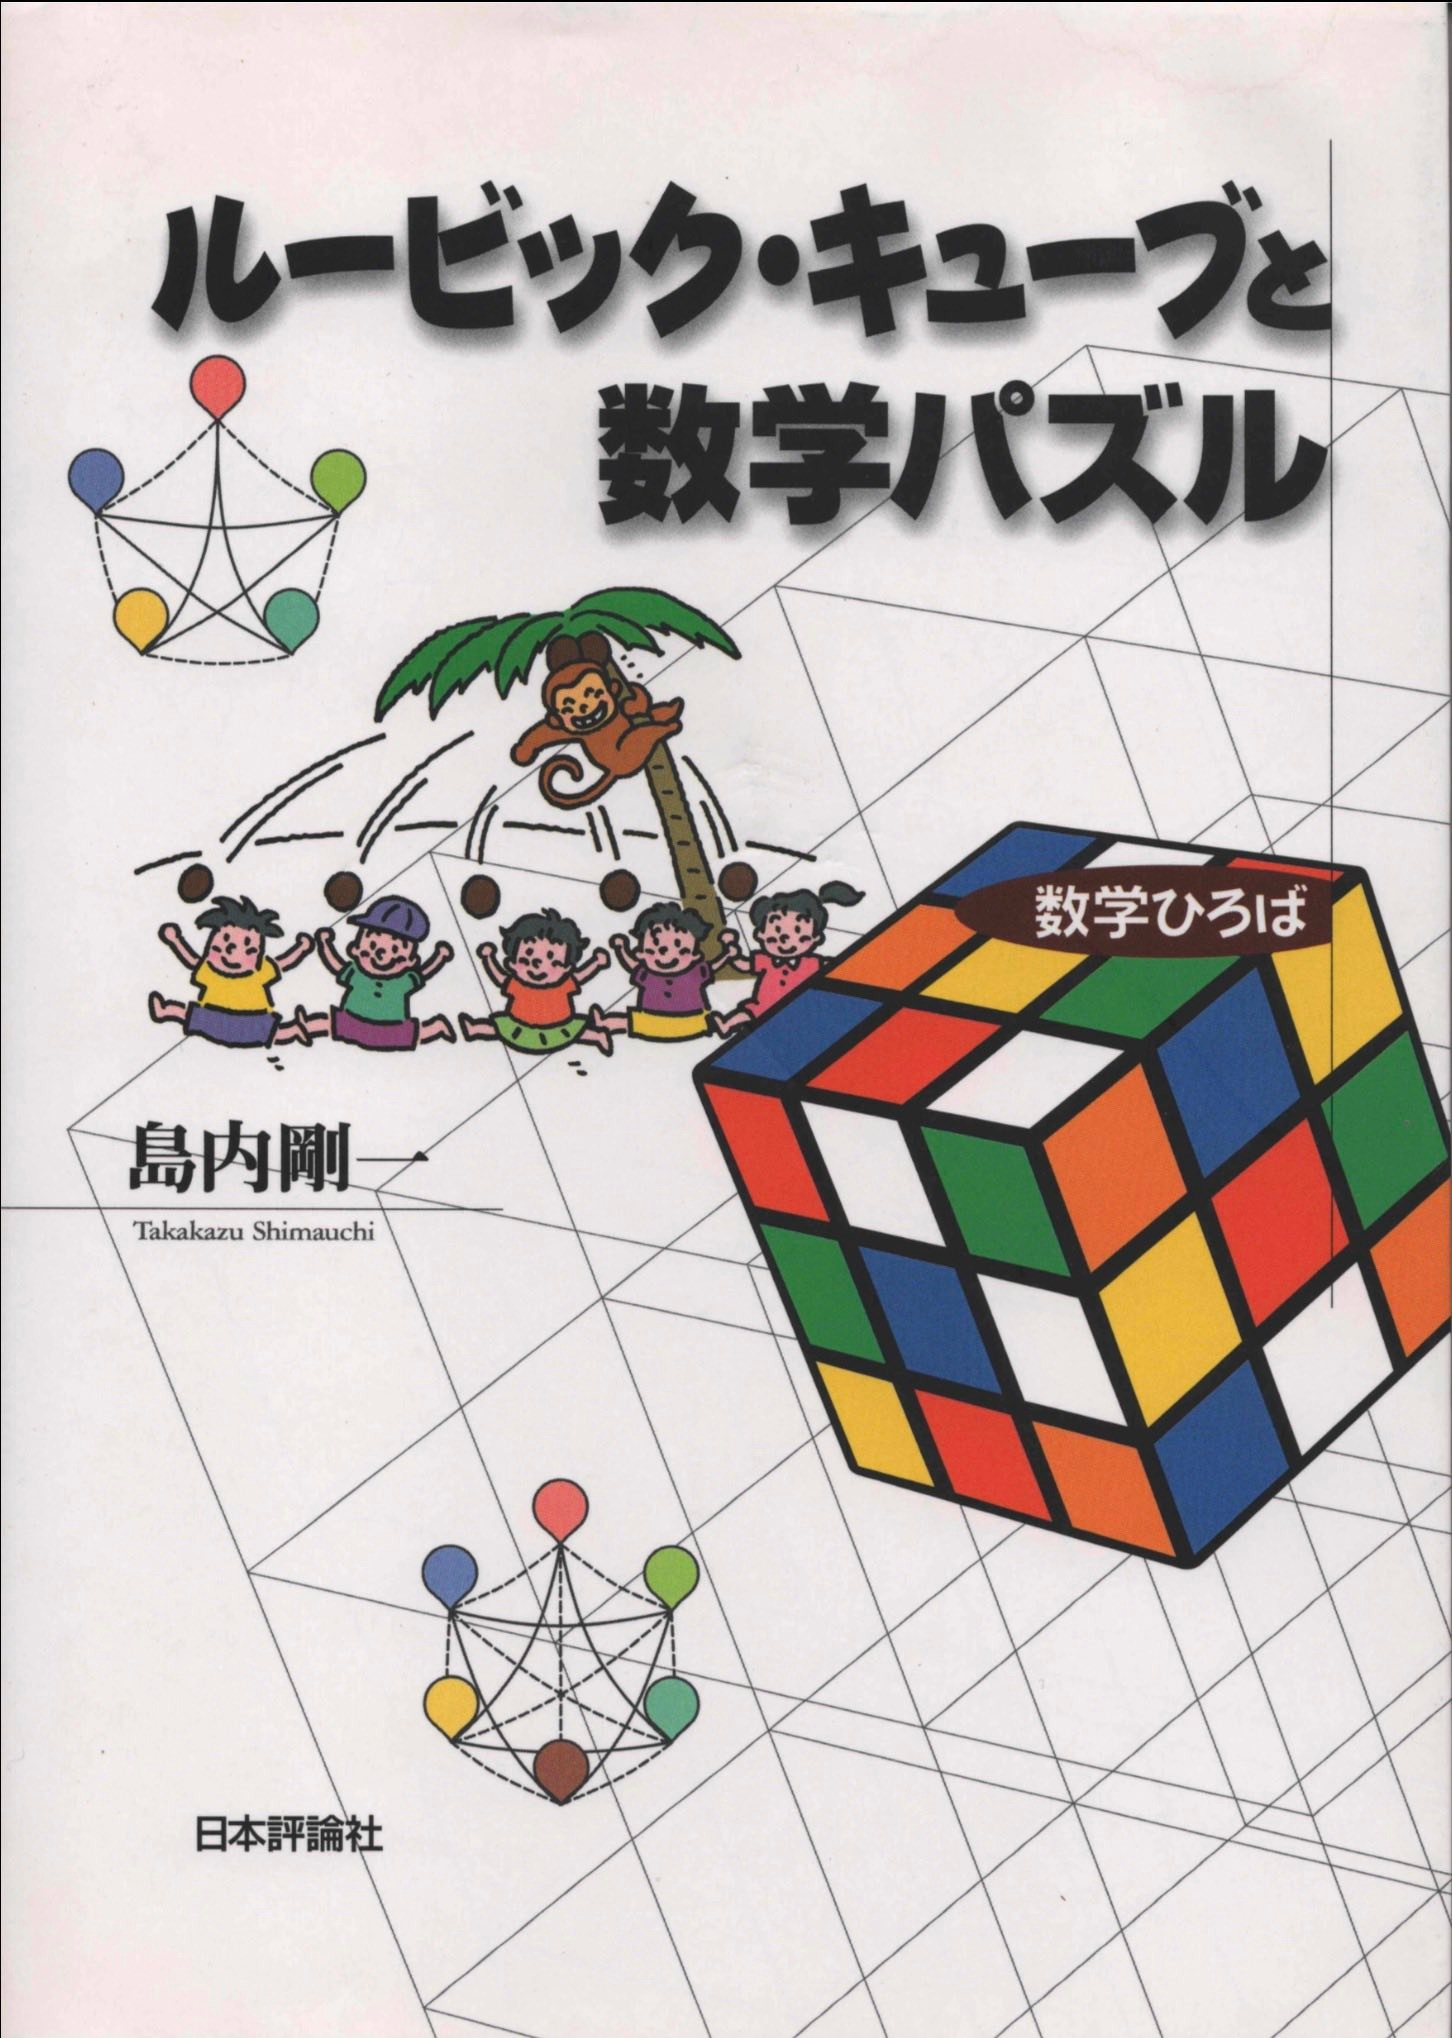
\includegraphics[width=\linewidth]{pictures/2026/03/20260328_013418_001.jpg}
\end{minipage}
\hfill
\begin{minipage}{0.48\linewidth}
\centering
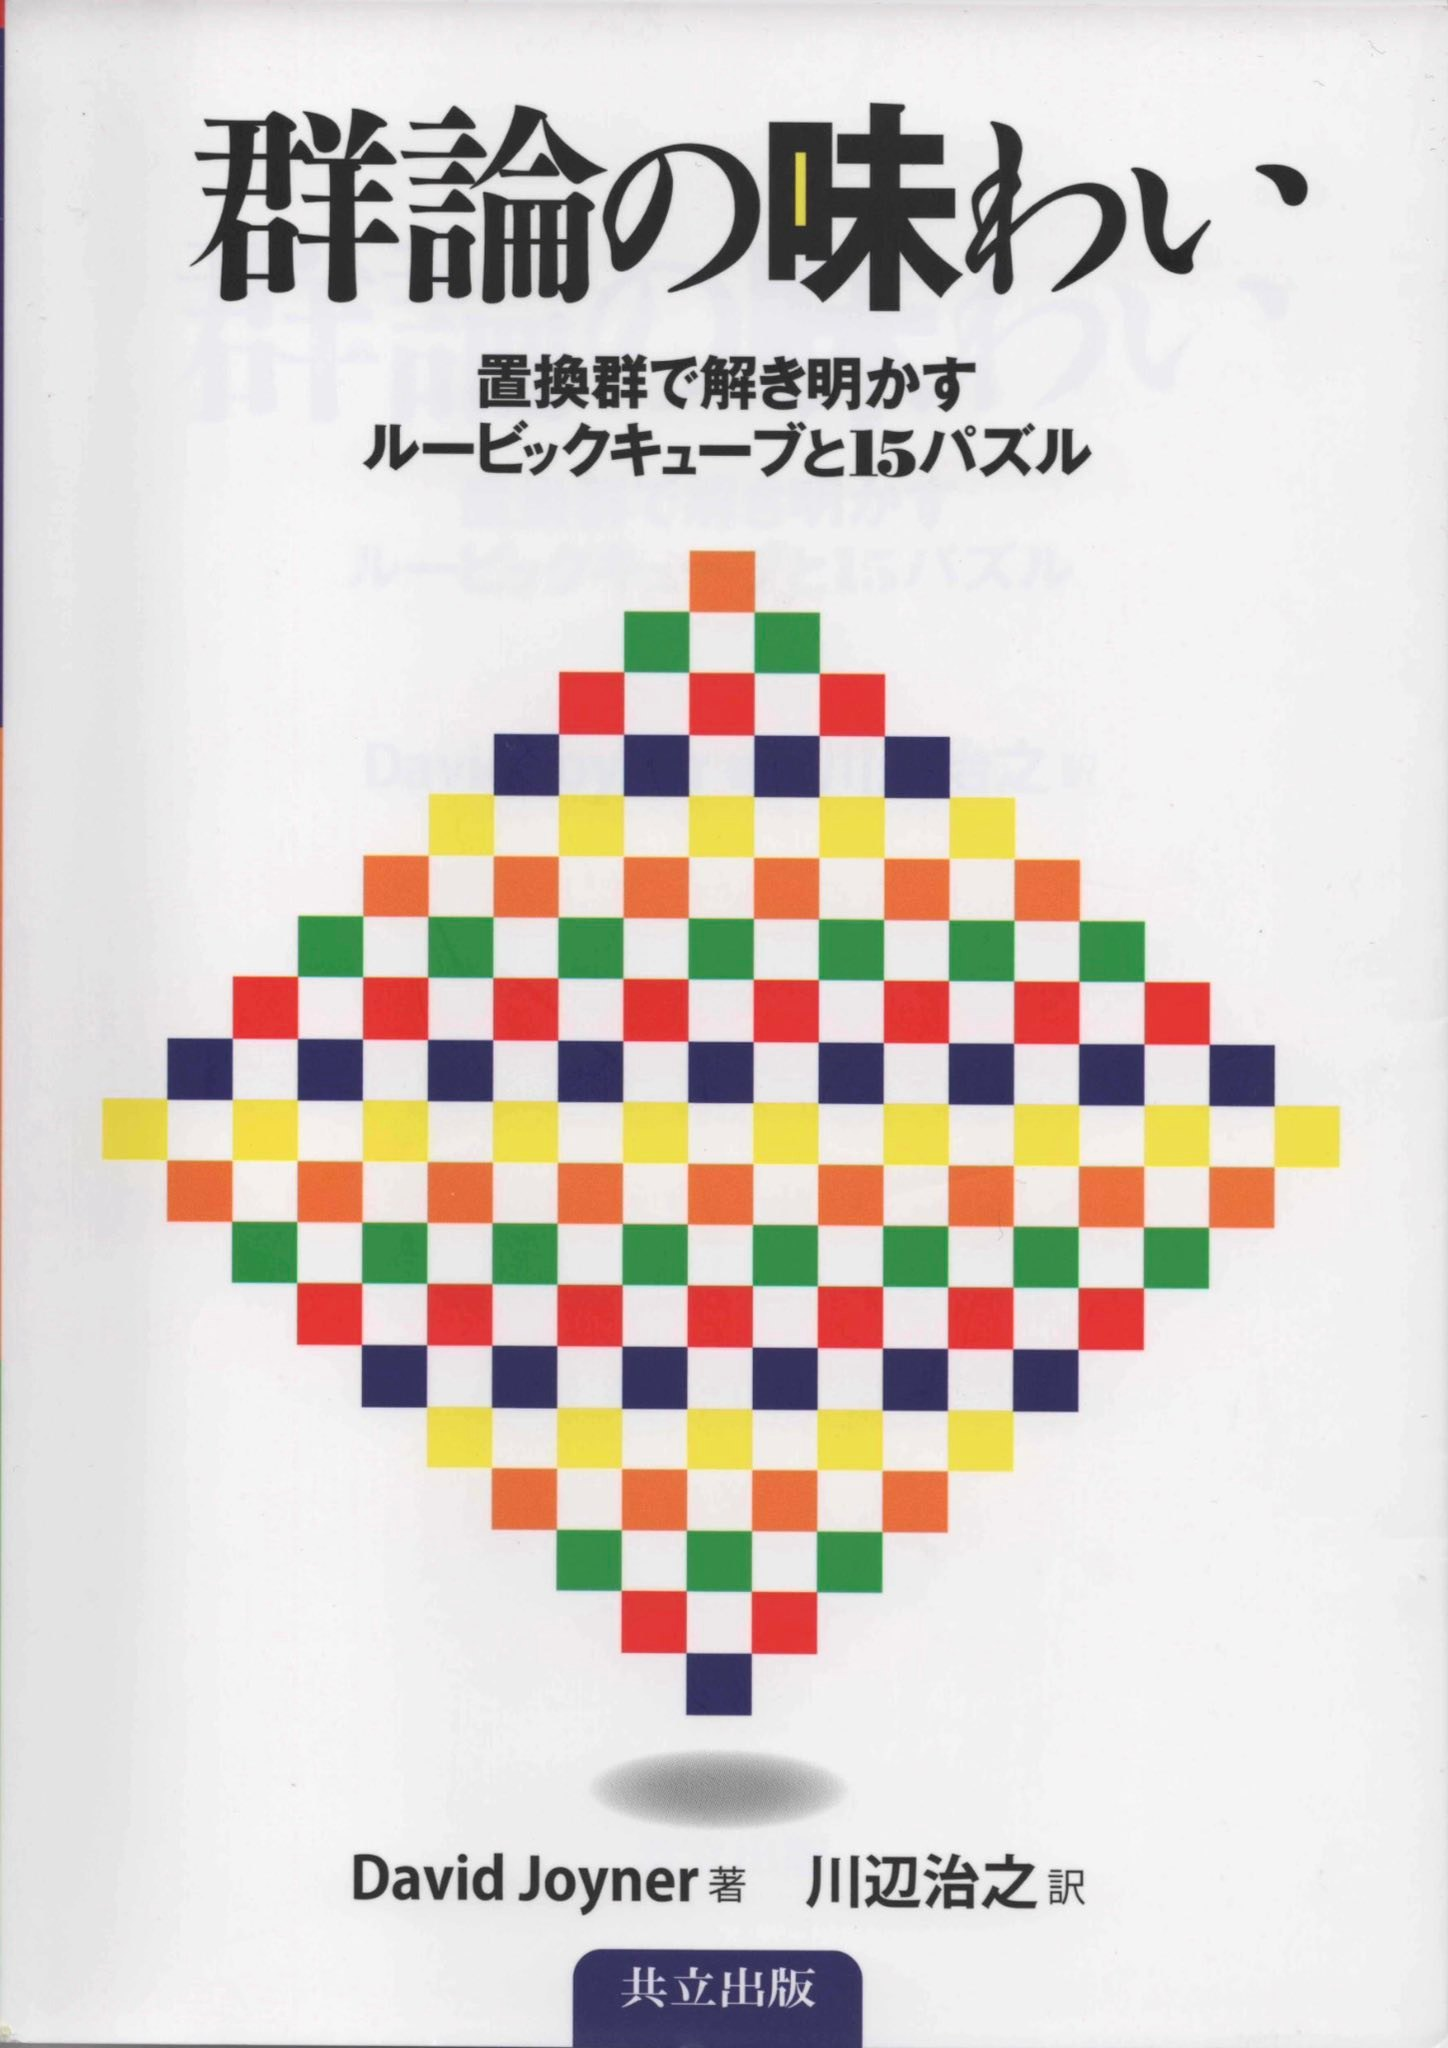
\includegraphics[width=\linewidth]{pictures/2026/03/20260328_013418_002.jpg}
\end{minipage}
\end{center}

\subsection*{2026年03月28日 08:38}
\addcontentsline{toc}{subsection}{2026年03月28日 08:38}

無伴奏チェロ組曲第６番よりSarabandeをやってみようと思いはじめた


ヘーゲル編と益田正洋編を比べてみると、明らかにヘーゲル編の方が音符がたくさん書かれている（益田編の方はシンプル）

一方、偶然見かけたファクシミリ譜の印象によれば、原曲はチェロの曲なので、一般的なギターの楽譜に比べると音符は少なくなっています（益田編の方が原曲に近い編曲になっているのではないか）


\url{https://youtu.be/06JzNQWJKOY}

\begin{center}
\href{https://youtu.be/06JzNQWJKOY}{
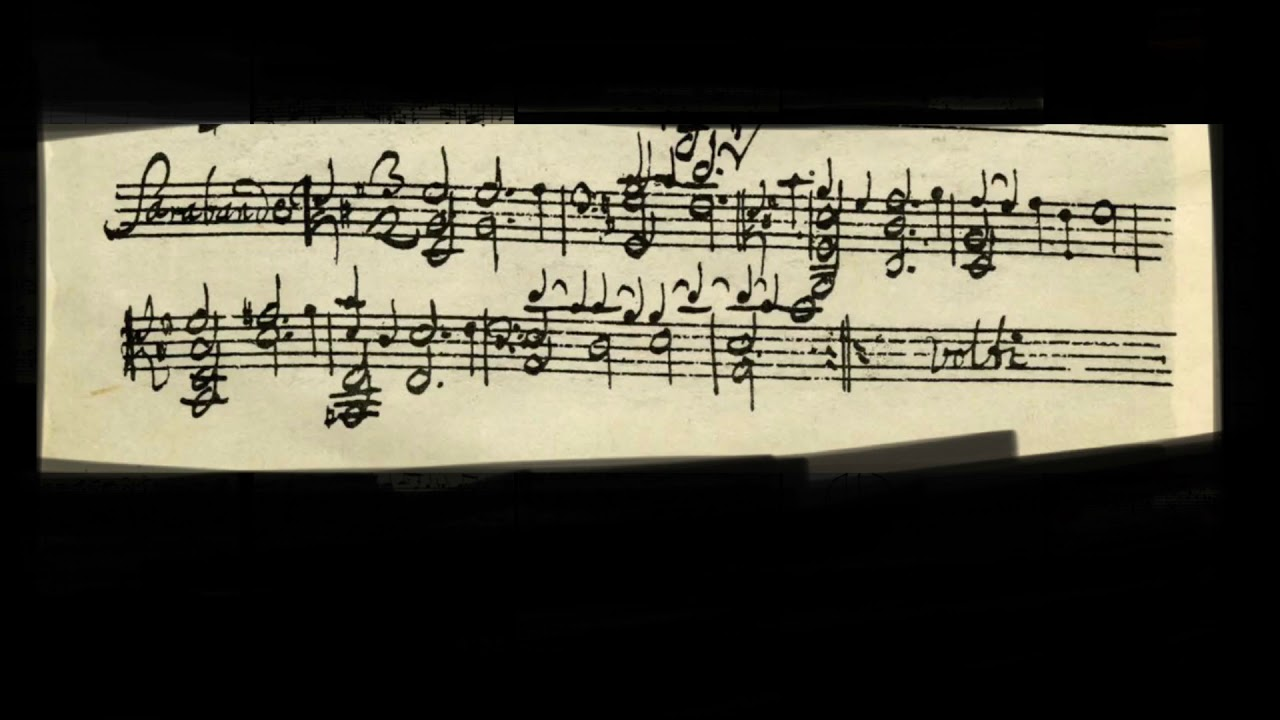
\includegraphics[width=0.48\linewidth]{pictures/youtube/2026/03/20260328_083856_youtube_001_06JzNQWJKOY.jpg}
}
\end{center}




そうすると、ヘーゲル編は何処から音を持ってきた（編み出してきた）ものでしょうか（幾つか鳴らしてみると、何とも和音の響きが魅力的なのだが）音を重ねる事によって、チェロの音の様な重々しさを出そうという狙いなのかも


さて、どの楽譜でいこうか？（短い曲ですし、とりあえず両方ともやってみる事にしようかな）最初は益田編で弾きはじめて、繰り返しはヘーゲル編で弾く、というのはどんなものでしょうか？（自分でアレンジした繰り返しを、、というワザは無理ですから、もしや、これってすごく良いアイデアなんじゃないかな？）


（その後）

うーん、ヘーゲル編ちょっとムズイぞ（音を音符通り残そうとすると指が届かない！←とりあえず、16小節目のバスは二分音符に、17小節目のベースの二分音符は四分音符＋四部休符に、勝手ながら、その様にさせて頂く事にします）

それでも、弾いていると、それはとても幸せなバッハの響き、音楽です（特にヘーゲル編）


===

以下↓の記事の続きです

\url{https://www.facebook.com/100002225117991/posts/24986489807675178/}



\paragraph{写真}
\begin{center}
\begin{minipage}{0.48\linewidth}
\centering
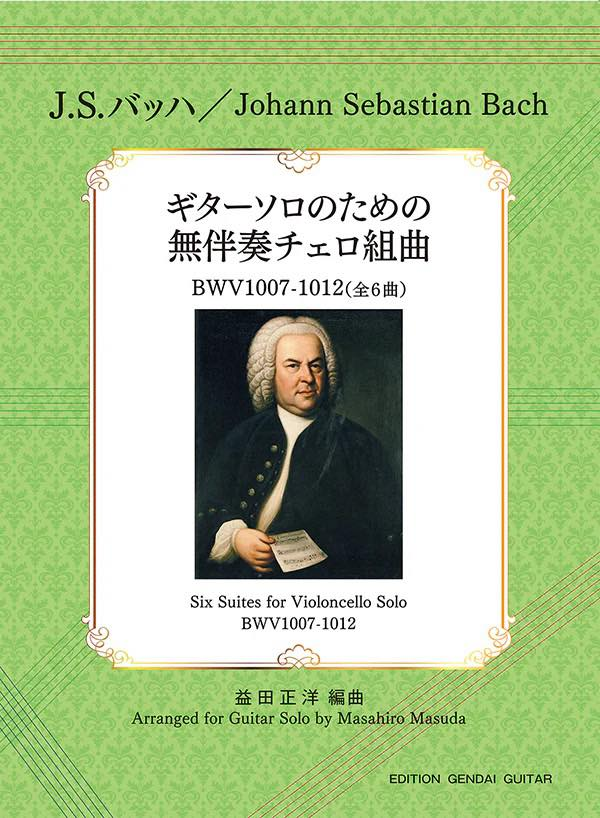
\includegraphics[width=\linewidth]{pictures/2026/03/20260328_083856_001.jpg}
\end{minipage}
\hfill
\begin{minipage}{0.48\linewidth}
\centering
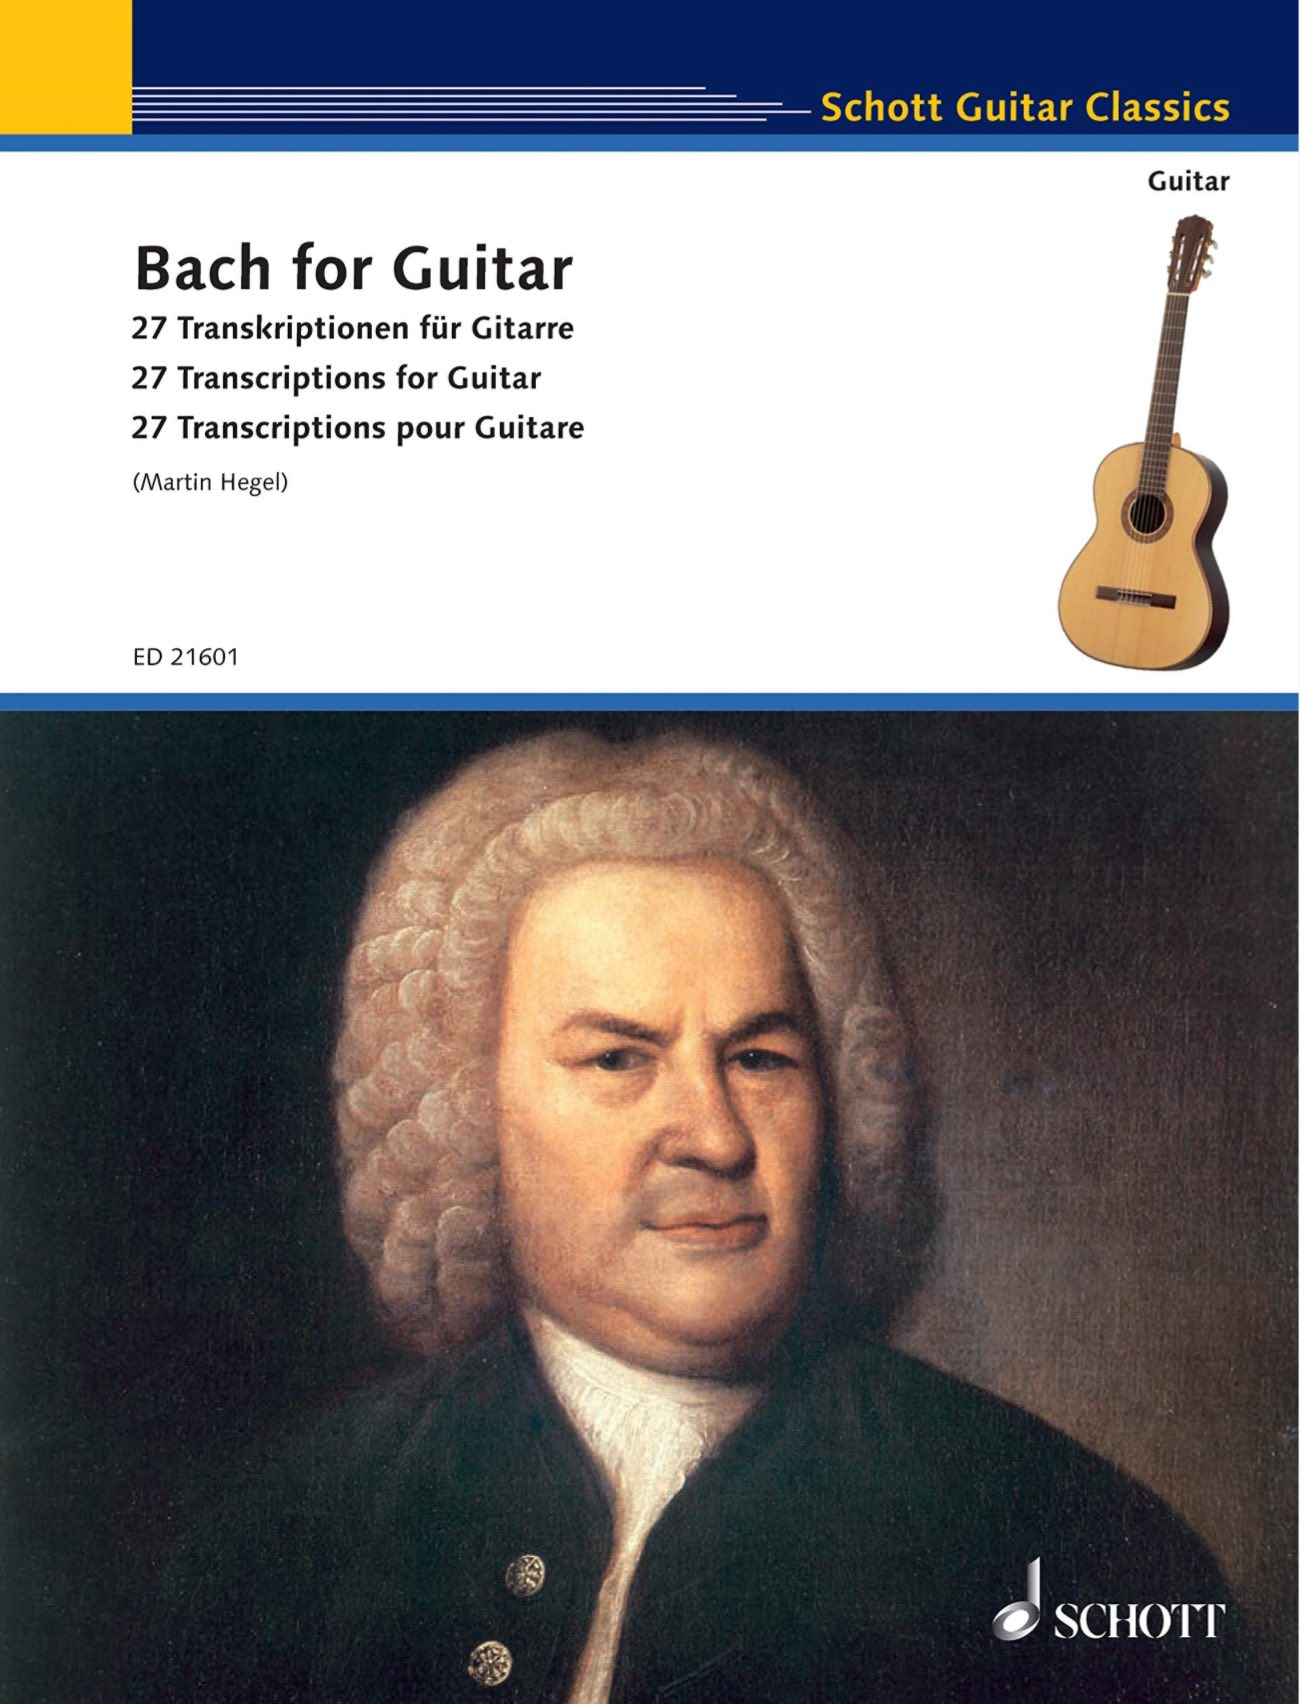
\includegraphics[width=\linewidth]{pictures/2026/03/20260328_083856_002.jpg}
\end{minipage}
\end{center}

\subsection*{2026年03月30日 17:58}
\addcontentsline{toc}{subsection}{2026年03月30日 17:58}

昔、お気に入りで頼りにしていました（今はどこにあるかな？）

必要に応じて参照して（辞書的に利用して）いた本です。


昔は、移流拡散の流れの場、分子軌道法、電磁気のベクトル場など等、色々書いて（描いて）きた様に思います。シミュレーションのプログラムをあれこれ書いていた当時、本当にお世話になった本です。


そもそもプログラムって、「曖昧な理解＝何となくこういう感じの様な気がする」では、書けないです。「掛け値無しで100\%完璧」な理解でないと、まともに動作するプログラムは、１行だって書き進めることはできません。←これって、言わずもがなの当たり前な事なのですが、「曖昧無しに」とは必ずしも容易な事ではありません。でも、流体力学だ、量子力学だ、電磁気学だといった諸々を、最初から最後まで100\%分かる必要はない（し、当然分かっていない）です。プログラムする時に必要な所（部分）に対してだけ、「逆戻りして調べて」理解して行くという作業が必要なんだと思います。


キチンと分かりたい者の「摘み食いニーズ」に応えてくれる本でした。（でも、教員には必要のない本でした）本当にどこへ行っちゃったんだろう、見当たらんなあ。


===

数物書籍関連

\url{https://m.facebook.com/story.php?story_fbid=25241325465524943&id=100002225117991}




\url{https://www.facebook.com/100002225117991/posts/5666106916806756/}



\paragraph{写真}
\begin{center}
\begin{minipage}{0.48\linewidth}
\centering
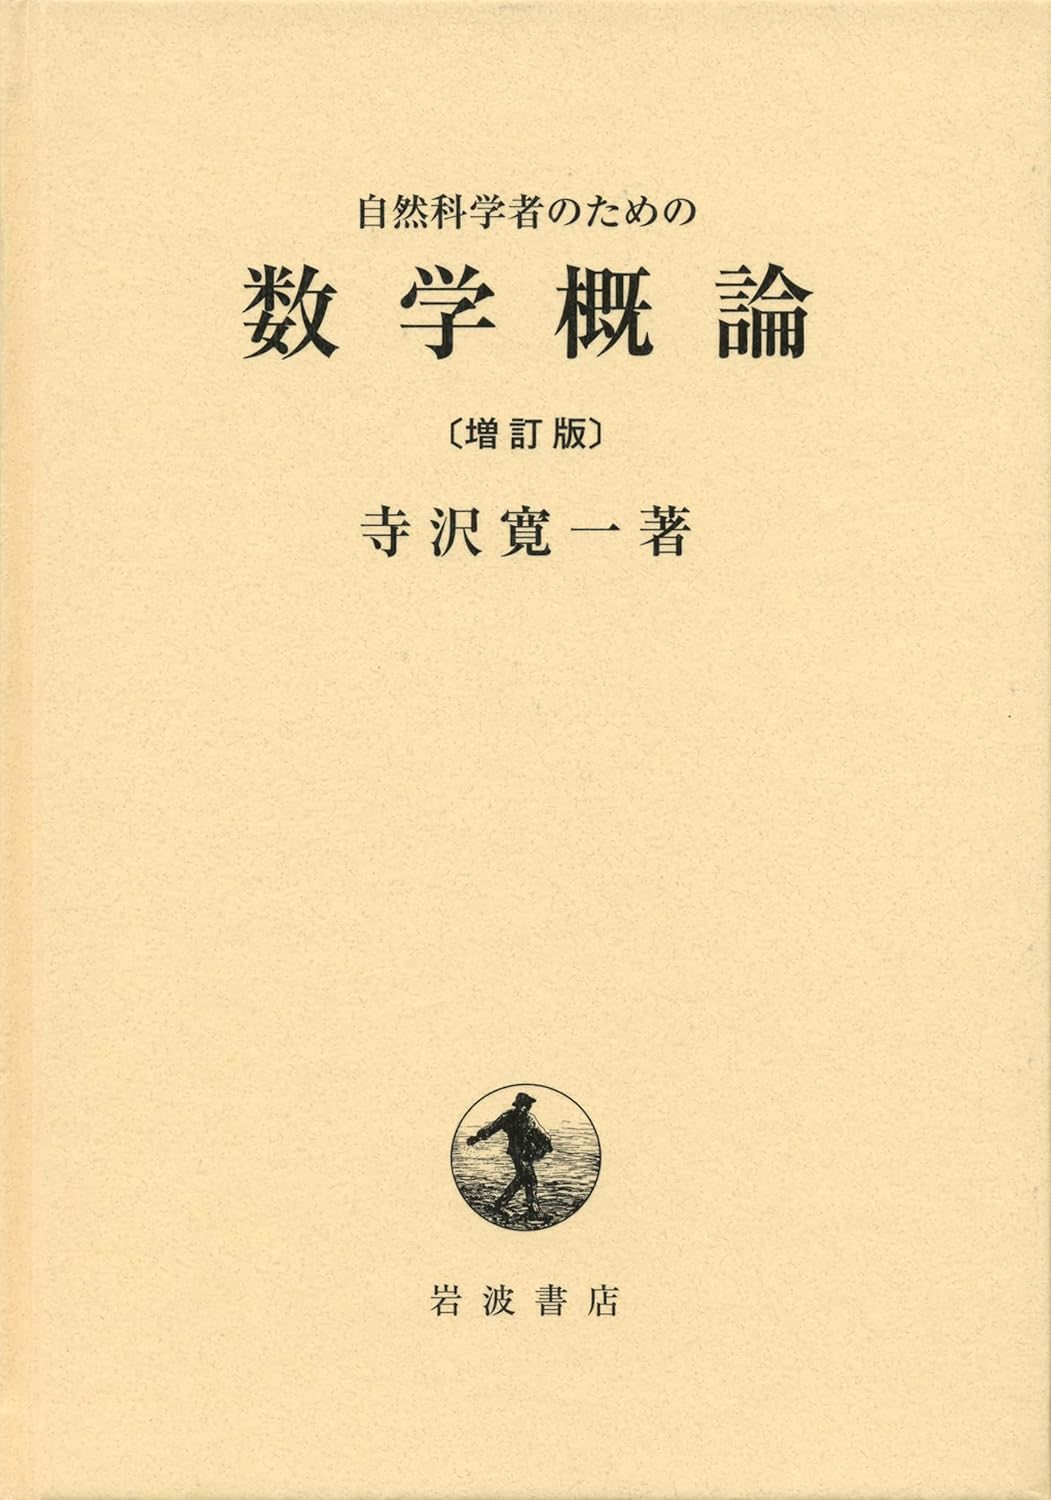
\includegraphics[width=\linewidth]{pictures/2026/03/20260330_175833_001.jpg}
\end{minipage}
\hfill
\begin{minipage}{0.48\linewidth}
\centering
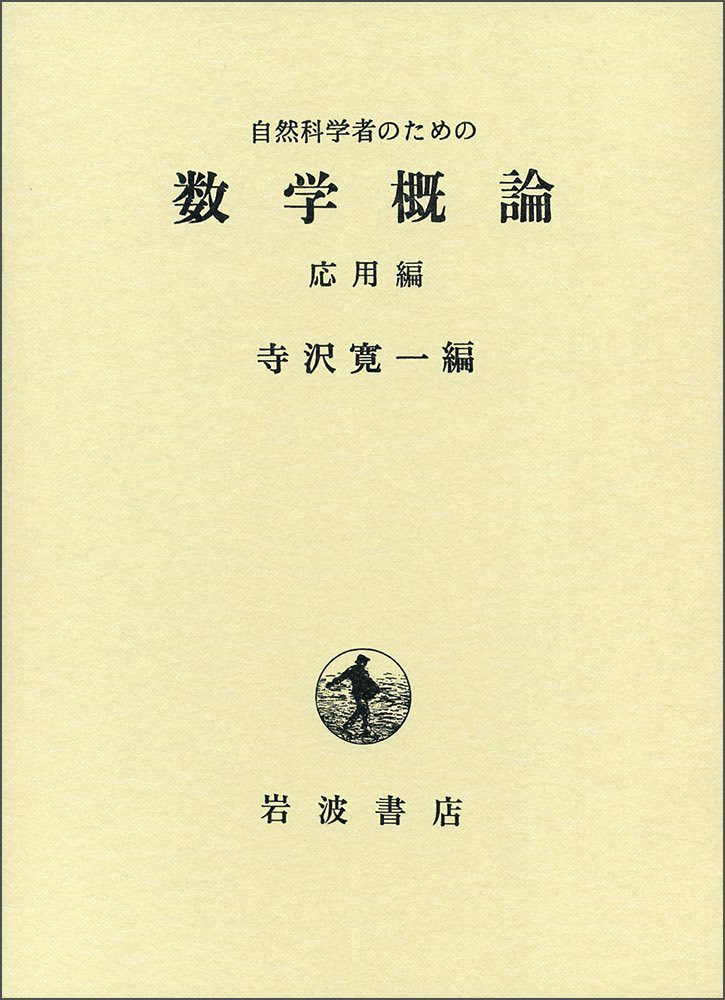
\includegraphics[width=\linewidth]{pictures/2026/03/20260330_175833_002.jpg}
\end{minipage}
\end{center}

\subsection*{2026年03月31日 18:57}
\addcontentsline{toc}{subsection}{2026年03月31日 18:57}

\paragraph{リンク}
\url{https://youtu.be/wV1F9KAuUW0}

\begin{center}
\href{https://youtu.be/wV1F9KAuUW0}{

\includegraphics[width=0.48\linewidth]{pictures/youtube/2026/03/20260331_185722_youtube_001_wV1F9KAuUW0.jpg}
}
\end{center}

\subsection*{2026年03月31日 19:53}
\addcontentsline{toc}{subsection}{2026年03月31日 19:53}

\paragraph{リンク}
\url{https://youtu.be/JSXJ-c4ML1I}

\begin{center}
\href{https://youtu.be/JSXJ-c4ML1I}{
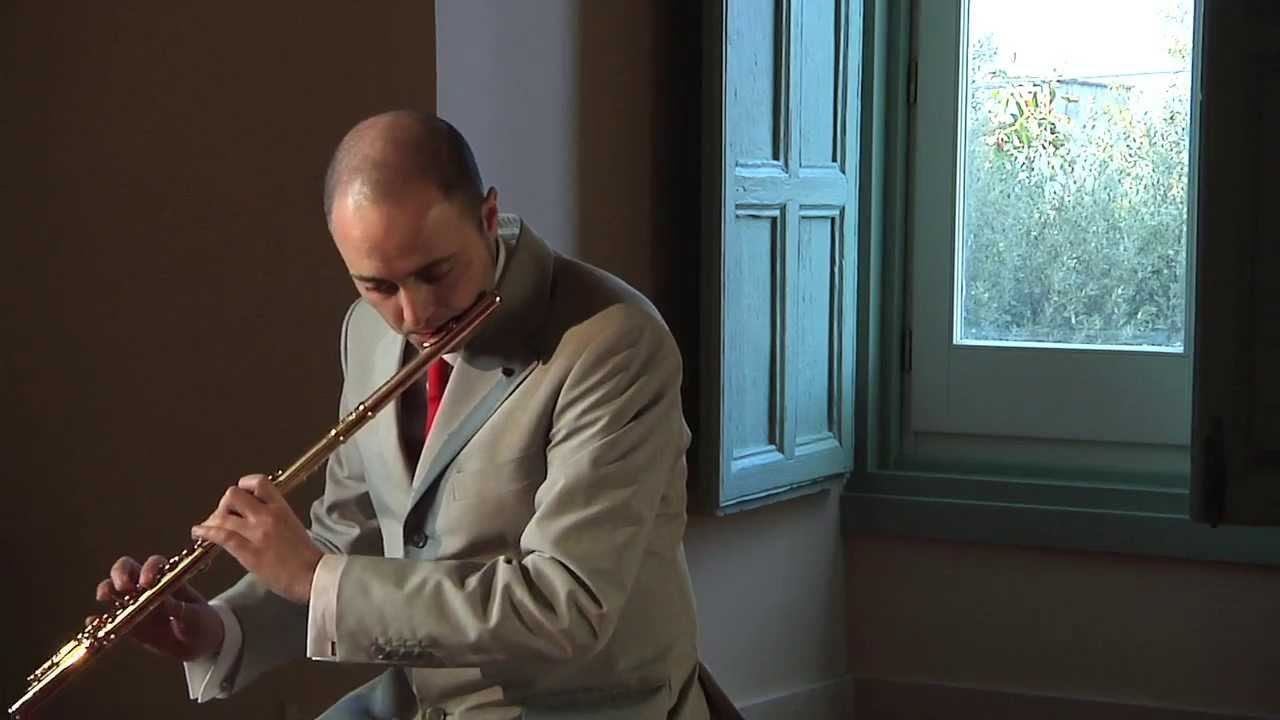
\includegraphics[width=0.48\linewidth]{pictures/youtube/2026/03/20260331_195312_youtube_001_JSXJ-c4ML1I.jpg}
}
\end{center}

\subsection*{2026年03月31日 19:54}
\addcontentsline{toc}{subsection}{2026年03月31日 19:54}

\paragraph{リンク}
\url{https://youtu.be/UM5_fEhzObI}

\begin{center}
\href{https://youtu.be/UM5_fEhzObI}{
\includegraphics[width=0.48\linewidth]{pictures/youtube/2026/03/20260331_195422_youtube_001_UM5_fEhzObI.jpg}
}
\end{center}

\section{4月}

\subsection*{2026年04月02日 02:45}
\addcontentsline{toc}{subsection}{2026年04月02日 02:45}

\paragraph{リンク}
\url{https://x.com/philosophyofphy/status/2039387566584082819}

\subsection*{2026年04月03日 00:56}
\addcontentsline{toc}{subsection}{2026年04月03日 00:56}

移流拡散方程式の数値解析（シミュレーション）


H社でスーパーコンピュータの研修を受けたことがありました。村田健郎先生や後先生の資料や講義でした。差分法そして大型連立方程式の反復解法（CG法など）について詳しく学ぶことができました。


村田先生はニコニコしながらの数学の講義が印象的でした。線形代数やルベーグ積分などの説明資料も手書きの詳しい資料で、分かりやすく話して下さいました。この時初めて数学が本当に理解できたという気になりました。数学ってこうやって読めば読めるんだ、という納得する感じがしましたよ。また、その頃（移流拡散方程式にハマっていた頃）は数学をあれこれ必要としておりましたので、この本（ 

\url{https://www.facebook.com/100002225117991/posts/26238155249175288/}

 ）はその都度助けになりました。

後（うしろ）先生は、共役勾配法のアルゴリズムを中心に話されていた様に思います。（東大の計算機センターのサポートでお忙しかった？）


その時の研修会では、指導者として関わってはいらっしゃいませんでしたが、H社には大型スパース行列の扱いや数値解析に関する著書を何冊も出していらっしゃる小国力氏もいらっしゃいました。実は私も同じ部に所属していたのですが、私の事はご存知なかったでしょうね（京浜東北線の電車の中でたまたまお会いして、ごあいさつ程度にお話しした事はありましたが）。丸善から次に出される本の執筆中だったのでしょうか、いつも（丸善の）原稿用紙に向かっていらしたのが印象的でした。


\url{https://x.com/mathelirium/status/2039715109002412252}




乱流は難しいんですよね（今はどんなモデル化が成されているんだろう）

当時のスーパーコンピュータ（ヴェクトル・プロセサ）でもこんな↑絵は作れなかったですよ。そもそもこんなに細かなメッシュを生成しての計算を、今はデスクトップに居て作れる時代なんですね。（時間方向の積分だって大変な事ですよ）

\subsection*{2026年04月03日 06:34}
\addcontentsline{toc}{subsection}{2026年04月03日 06:34}

これは公開しない


自分がそうでした


\url{https://www.asahi.com/articles/ASV3Z165NV3ZUPQJ00WM.html?ref=facebook}




自分の思いを話し始めようとすると、「まだそんな事言ってるの」「一期校に受かってるんだから、行けばいいじゃない」「何を不満ばかり言ってるの、受かっていない人だっているんだよ」「とにかく今の大学行って」という感じ。初っ端から話を聞いて貰える様な状態じゃなかった。私が話し始める前に、答え（反応）は決まっていました。壁から跳ね返される様な感じでした。また、今の時代であれば、その後の進路も含めてかなりフレキシブルに選択していける様な気もしますが、当時はそうではなかったと思います。


でも一旦は予備校に行こうとしました。近畿予備校の校舎は京都御所の向かいにありました（今はもう無いのか？）。予備校への入学（？）手続きのために京都駅から校舎まで烏丸通りを歩きました（今思えば遠い）。烏丸を「からすま」と読むのは、自分が「る」を聞き落としているのかも、と思っていました。どこまで歩いても続いていたのは、いったい誰の家だろうと思ったら御所でした。地下鉄が出来ていなくて、その頃は丁度道路を掘り起こしての工事中でした。予備校の手続きの時に窓口の方から、「しっかり勉強しないと点数悪いよ」と言われました。二階の広い部屋でテキスト販売がありましたが、そこで会った業者の方が、高校の英語の先生の名前をあげて「⚪︎⚪︎先生の高校だね」と言われたので、びっくりしました。

一方、大学の入学手続きも進めていました。いわゆる仮面浪人を画策していたので。教養部の授業の学修票提出期限があって大変でした。そして結局、京都の予備校に行くのをやめてしまいました。大学生活のぬるま湯に浸かってしまったという事だと思います。最終的に自分で選んだ道だったという事です。


大学卒業の頃に、卒論の指導をして下さっていた先生が、先生の部屋で私の話を黙って最後まで聞いて下さいました。人に私の思いを最後まで聞いてもらったのは初めての事でした。話した事は、自分一人でいつも心の中で反芻していた後悔の気持ちでした。最後まで話終わった時ようやく心の中がホッとしました。初めて（壁で跳ね返されるのではなくて）受けとめてもらえた気がした事で、その場で心が穏やかに落ち着いていったのが分かりました。卒業する頃になってようやく立ち直ることができたという感じだったでしょうか。入学時に思いを吐露できていたら違った学生時代ではあったかもしません。（でも、これは反実仮想ですよ。どうだったかは分かりませんね。）


基本はじっと「最後まで」話を聞く事なんだ（カウンセリング・マインド）という事に納得する様な出来事でした


===

以下に続く（かも）

\url{https://www.facebook.com/100002225117991/posts/9971443412939730/}



\paragraph{写真}
\begin{center}
\begin{minipage}{0.48\linewidth}
\centering
\includegraphics[width=\linewidth]{pictures/2026/04/20260403_063452_001.jpg}
\end{minipage}
\end{center}

\subsection*{2026年04月03日 09:03}
\addcontentsline{toc}{subsection}{2026年04月03日 09:03}

\paragraph{リンク}
\url{https://youtu.be/EXqpK5MDXFI}

\begin{center}
\href{https://youtu.be/EXqpK5MDXFI}{
\includegraphics[width=0.48\linewidth]{pictures/youtube/2026/04/20260403_090328_youtube_001_EXqpK5MDXFI.jpg}
}
\end{center}

\subsection*{2026年04月04日 09:53}
\addcontentsline{toc}{subsection}{2026年04月04日 09:53}

\paragraph{リンク}
\url{https://youtu.be/WEHf584ed8Y}

\begin{center}
\href{https://youtu.be/WEHf584ed8Y}{
\includegraphics[width=0.48\linewidth]{pictures/youtube/2026/04/20260404_095327_youtube_001_WEHf584ed8Y.jpg}
}
\end{center}

\subsection*{2026年04月04日 13:26}
\addcontentsline{toc}{subsection}{2026年04月04日 13:26}

\paragraph{リンク}
\url{https://youtu.be/v5WMKyFKvr8}

\begin{center}
\href{https://youtu.be/v5WMKyFKvr8}{
\includegraphics[width=0.48\linewidth]{pictures/youtube/2026/04/20260404_132639_youtube_001_v5WMKyFKvr8.jpg}
}
\end{center}

\subsection*{2026年04月04日 18:35}
\addcontentsline{toc}{subsection}{2026年04月04日 18:35}

演奏していらっしゃる方のスキルに加えて、楽器も澄んだいい音している様な気がします。多少エコーがかけられているかもしれませんが、聞いていて気持ちいい音です。音程がいいと言うのも原因の一つかもしれません。（フルートで音程が良いとは、モーツァルトに聞かせてあげたい所です）


\url{https://youtu.be/oH5GcQHIPAc}

\begin{center}
\href{https://youtu.be/oH5GcQHIPAc}{
\includegraphics[width=0.48\linewidth]{pictures/youtube/2026/04/20260404_183505_youtube_001_oH5GcQHIPAc.jpg}
}
\end{center}




私が所有している（大切にしている）楽器は、昔サンキョウが数を限って販売していた時のコーカスウッド製です。コーカスウッドという木材は、今となってはもう枯渇してしまっているらしいですから、この木材で作られた楽器は、もう容易には手に入らないものと思います。

ここで演奏に使われている楽器は、私の持っている（貴重な）楽器と見かけはそっくりな様ですが、（最近手に入れられた楽器であるならば）モパネという木材によるものかもしれません。最近サンキョウが売り出しているみたいです。おそらくコーカスウッドに代わる木材として探され、開発された楽器なのだろうと推察します。（それにしても高価になっちゃったものです。）


\url{https://jp.sankyoflute.com/catalog/otherindex.html}




グラナディラも今後枯渇しそうだと聞いたことがありますし、ヴァイオリンなどの弦楽器の弓に使われている木材も、既に手に入らなくなってきていると聞いています。林業による計画的な木の育成と、それこそ計画的な消費が望まれる所ですが、、、もう手遅れなのか？

\subsection*{2026年04月05日 05:42}
\addcontentsline{toc}{subsection}{2026年04月05日 05:42}

メモ


\url{https://m.facebook.com/story.php?story_fbid=1638871220486279&id=100030902512100}



\subsection*{2026年04月05日 06:39}
\addcontentsline{toc}{subsection}{2026年04月05日 06:39}

\paragraph{リンク}
\url{https://x.com/mathelirium/status/2039715109002412252}

\subsection*{2026年04月05日 09:29}
\addcontentsline{toc}{subsection}{2026年04月05日 09:29}

\paragraph{リンク}
\url{https://x.com/mathelirium/status/2040368874160304553}

\subsection*{2026年04月06日 03:40}
\addcontentsline{toc}{subsection}{2026年04月06日 03:40}

The Westminster Chimes

( 

\url{https://fb.watch/GiptiRNPiE/?fs=e}

 )

( 

\url{https://fb.watch/GiurHU7LZH/?fs=e}

 )


First used on the clock at Great St. Mary’s, Cambridge, these were originally called the Cambridge Chimes and are derived from Handel’s ‘Messiah’.

Now famous because of their adoption at Westminster, they are known as the Westminster Chimes.

The bells are turned to the key of F major with the hour bell( Big Ben) sounding note E.

( 

\url{https://web.mit.edu/kenta/www/three/westminster/chimes.html}

 )

\paragraph{写真}
\begin{center}
\begin{minipage}{0.48\linewidth}
\centering
\includegraphics[width=\linewidth]{pictures/2026/04/20260406_034008_001.jpg}
\end{minipage}
\end{center}

\subsection*{2026年04月06日 18:39}
\addcontentsline{toc}{subsection}{2026年04月06日 18:39}

メモ👀


\url{https://x.com/valaafshar/status/2040810294113350137}



\paragraph{リンク}
\url{https://x.com/valaafshar/status/2040810294113350137?s=61&t=5VtsOkpki6juEjPXsBq8hg}

\subsection*{2026年04月06日 18:46}
\addcontentsline{toc}{subsection}{2026年04月06日 18:46}

メモ👀


\url{https://x.com/technmak/status/2058189129717096655?s=61&t=5VtsOkpki6juEjPXsBq8hg}




ヤコビアン・マトリクス


tuとtvの外積が（単位）法線ベクトルn

\paragraph{写真}
\begin{center}
\begin{minipage}{0.48\linewidth}
\centering
\includegraphics[width=\linewidth]{pictures/2026/04/20260406_184651_001.jpg}
\end{minipage}
\end{center}

\subsection*{2026年04月06日 18:49}
\addcontentsline{toc}{subsection}{2026年04月06日 18:49}

面白い式も有りますね〜

なるほど〜と思ってみたりするのがいいですね

Math Clockはちょっと単純過ぎ＝つまんない？=>これ位が丁度いいか。5時はハテ、どうなんだ？3125って5の5乗なのかな？（というより、ここが5時だと言うのなら、3125は5の5乗でなければならない、ですね）

他の二つの時計は色々と予備知識が必要なものもあるね。微分と積分は、黙ってとにかく計算してみれば、と言う事かな。（分からないの幾つある？）

Chronos of Mathematica（文字盤の背景はマンデルブロー集合）は比較的お気に入りだが、イマイチだなと思ってしまうのは、普通に実数計算させておいて小数点以下を丸めろと言うもの（1時と7時）はどうなのか。3.14を2.71で割って切り捨てると1になるとは思いますが、2.71x2.71の結果を切り捨てると7になるとパッと分かるものなのかな？二進数の2時はオヤっと思ったし、列ベクトルでノルムの5時はなるほどと思いました。φはオイラー関数か。σは何だ？統計の話じゃないですよね。


（その後）

よく考えたら、これが時計だと思えば「ある程度暗算でできて整数が出てくる」というのは必要な事かもしれません。その意味では、二項係数や2x2の行列式、冪乗や階乗、ノルム、二進数、無限等比級数というのは👍いいねという気がする（でも、二項係数は3時の１箇所でいいよ。11時はCombinationの11C10にして下さい。）4時のオイラー関数φ(8)は、一回数えてみなくちゃいけない「8と共通の素因数を持たない8以下の自然数の個数」は、1、3、5、7の４個。π（関数）では17以下の素数の数で、2,3,5,7,11,13,17の7個、それを7時に。それにしてもσは何？

\paragraph{写真}
\begin{center}
\begin{minipage}{0.48\linewidth}
\centering
\includegraphics[width=\linewidth]{pictures/2026/04/20260406_184942_001.jpg}
\end{minipage}
\hfill
\begin{minipage}{0.48\linewidth}
\centering
\includegraphics[width=\linewidth]{pictures/2026/04/20260406_184942_002.jpg}
\end{minipage}
\end{center}

\begin{center}
\begin{minipage}{0.48\linewidth}
\centering
\includegraphics[width=\linewidth]{pictures/2026/04/20260406_184942_003.jpg}
\end{minipage}
\hfill
\begin{minipage}{0.48\linewidth}
\centering
\includegraphics[width=\linewidth]{pictures/2026/04/20260406_184942_004.jpg}
\end{minipage}
\end{center}

\subsection*{2026年04月07日 12:55}
\addcontentsline{toc}{subsection}{2026年04月07日 12:55}

メモ（ストークスの定理）


\url{https://x.com/mathemetica/status/2041173174159851531}



\paragraph{リンク}
\url{https://x.com/mathemetica/status/2041173174159851531?s=61&t=5VtsOkpki6juEjPXsBq8hg}

\subsection*{2026年04月07日 13:22}
\addcontentsline{toc}{subsection}{2026年04月07日 13:22}

（他人事だけど）大学の役割について「その通りかもしれん」と言う気がします


\url{https://ashidahironao.sakura.ne.jp/blog/cat35/post-505.html?fbclid=IwZnRzaARItR9leHRuA2FlbQIxMQBzcnRjBmFwcF9pZA8xNzM4NDc2NDI2NzAzNzAAAR5ynNnJBr40sd1Re-Em2C8kV3dirCsS6jW_uuJCcoJ-8_MKyywf9aYcd-sapg_aem_xu5fXsEhNY5-AMd2YnT99g}




少なくとも、「（研究は難しいけど）教育ならできる」と言う方がいらしたとしたら、おそらくは、教育「も」できない方だろうと推察します。


リンク先の記事とは直接関係ないけど、大学の学部レベルでの教授内容に関する政策ついて疑問に思うことは色々ある


(１)教授内容を没個性なYoutube番組にしてしまう様な政策（学部単位の評価レベル付け）

(２)教授内容を単なる資格取得対策講座にして、専門学校の目的と一緒にしてしまう様な政策

(３)論文を書いたことのない脱サラリーマンや芸能人を、教授と同列に扱おうとする政策

\paragraph{リンク}
\url{https://ashidahironao.sakura.ne.jp/blog/cat35/post-505.html}

\subsection*{2026年04月07日 17:42}
\addcontentsline{toc}{subsection}{2026年04月07日 17:42}

シュレーディンガー方程式の視覚化


\url{https://x.com/philosophyofphy/status/2041363585784549690}




\url{https://x.com/pickover/status/2041877779793252567}




\url{https://commons.wikimedia.org/wiki/File:Wavepacket-a2k4-en_(2X_speed}

).gif

\paragraph{リンク}
\url{https://x.com/philosophyofphy/status/2041363585784549690?s=61&t=5VtsOkpki6juEjPXsBq8hg}

\subsection*{2026年04月07日 17:42}
\addcontentsline{toc}{subsection}{2026年04月07日 17:42}

\paragraph{リンク}
\url{https://x.com/philosophyofphy/status/2041363585784549690?s=61&t=5VtsOkpki6juEjPXsBq8hg}

\subsection*{2026年04月08日 15:47}
\addcontentsline{toc}{subsection}{2026年04月08日 15:47}

\paragraph{リンク}
\url{https://x.com/yasunomu1/status/2041755727065444366}

\subsection*{2026年04月10日 10:15}
\addcontentsline{toc}{subsection}{2026年04月10日 10:15}

稀代のMelody Maker 、ヘンデルの誕生日は？


\url{https://www.facebook.com/reel/886617724158771/?fs=e&fs=e}




ChatGPTによると、===ここから


ヘンデル（George Frideric Handel）は、バロック時代を代表する作曲家

生年月日：1685年2月23日（グレゴリオ暦換算では3月6日ともされる）

没年月日：1759年4月14日

出身地：神聖ローマ帝国（現ドイツ）のハレ


一部資料では、洗礼記録に基づいて2月24日とする説や、文献による日付に混乱が見られるが、現代では2月23日が一般的。多くの音楽関係のメディアや団体でヘンデルの生誕日として祝われている。


===ここまで


「稀代のメロディー・メーカー」は、印象的な旋律（メロディ）を生み出すアーティストを称賛する言葉ですが、これは作曲家ヘンデルに対する個人的な印象です。


グレゴリオ暦に換算された日付って、あまり顧みられないものなのかな？


これは、以下の記事の続きです

\url{https://m.facebook.com/story.php?story_fbid=26138337095823771&id=100002225117991}



\subsection*{2026年04月11日 06:16}
\addcontentsline{toc}{subsection}{2026年04月11日 06:16}

「ギターでマタイ受難曲」を探している


(１) Erbarme dich

\url{https://www.facebook.com/100002225117991/posts/25743405738650244/}




(２)O sacred head, Now Wounded

\url{https://www.facebook.com/100002225117991/posts/25730484673275684/}




(３) Aus Liebe

\url{https://www.facebook.com/100002225117991/posts/26363754339948711/}



\subsection*{2026年04月11日 06:25}
\addcontentsline{toc}{subsection}{2026年04月11日 06:25}

\paragraph{リンク}
\url{https://youtu.be/rwHPWGPscDA}

\begin{center}
\href{https://youtu.be/rwHPWGPscDA}{
\includegraphics[width=0.48\linewidth]{pictures/youtube/2026/04/20260411_062556_youtube_001_rwHPWGPscDA.jpg}
}
\end{center}

\subsection*{2026年04月11日 08:36}
\addcontentsline{toc}{subsection}{2026年04月11日 08:36}

マタイ受難曲よりAus Liebe


\url{https://youtu.be/pfp2auhX26w}

\begin{center}
\href{https://youtu.be/pfp2auhX26w}{
\includegraphics[width=0.48\linewidth]{pictures/youtube/2026/04/20260411_083637_youtube_001_pfp2auhX26w.jpg}
}
\end{center}




伴奏と歌を一人で弾こうとしているので、ちょっと大変そうだ（寧ろトラベルソのレパートリーとして、ギターと合わせるというのはどうかな？）

楽譜は見当たらない


===

「ギターでマタイ受難曲」はここ↓

\url{https://m.facebook.com/story.php?story_fbid=26362889510035194&id=100002225117991}



\subsection*{2026年04月11日 08:39}
\addcontentsline{toc}{subsection}{2026年04月11日 08:39}

\paragraph{リンク}
\url{https://youtu.be/R4uTDZMFSg8}

\begin{center}
\href{https://youtu.be/R4uTDZMFSg8}{
\includegraphics[width=0.48\linewidth]{pictures/youtube/2026/04/20260411_083957_youtube_001_R4uTDZMFSg8.jpg}
}
\end{center}

\subsection*{2026年04月11日 18:00}
\addcontentsline{toc}{subsection}{2026年04月11日 18:00}

今日（4月11日）朝日新聞の天声人語で語られている「主題とは異なる」けど、関連する話として。読んでいて思い出しました。そう言えば、この話（’Wow’ signalの件）は確か、以前読んでみていた旺文社の英検準一級「文単」に載っていた（Answering the Wow! Signal）という記憶が、、、


本箱探してたら、ありました。案外初めの方に載っている話題だったんだな。英単語などには覚えがないのに、話しの内容だけは頭の隅に残っていたという事か、、、(\textasciicircum{}\textasciicircum{};;

\paragraph{写真}
\begin{center}
\begin{minipage}{0.48\linewidth}
\centering
\includegraphics[width=\linewidth]{pictures/2026/04/20260411_180047_001.jpg}
\end{minipage}
\end{center}

\subsection*{2026年04月11日 23:25}
\addcontentsline{toc}{subsection}{2026年04月11日 23:25}

山登りの（仮想）計画


山登りのアプリを調べているとYamaRecoというのがよさげだった。実は、YAMAP というアプリの方がメジャーそうなんだけど、画面が何だかごちゃごちゃしていて、シンプルな方のアプリを選ぼうという気になった。


試しにアプリを使ってみようと思って、昔から気になっていた（京都の）大文字山に登るという（仮想）計画を立ててみることにした。電車で昼頃に京都に着けば、午後半日で登って降りてこられる計画にできるんじゃないかと思って（案外本当に行くつもりで）検討してみた。（現在の私の体力レベルではギリギリかもと思っていますが、Youtubeでは比較的高齢な方でも登っていらっしゃるみたいです）


銀閣寺からの最もポピュラーな登山口から入って、大文字の火床、大文字山の山頂を経て、再び火床を経由し、法然院に降りてこようというルートです。法然院に降りるというのは、それ程知られたコースでもない様なのですが、登りと全く同じ道を戻るというのも嫌でしたし、以前哲学の道から入った法然院の静寂（ 

\url{https://www.facebook.com/reel/1281757787418225/}

 ）が素晴らしかったので（お気に入りという事で）そこに向かう様にしてみました。（仮想ではなく、本当に登りに行きたいという気に、だんだんなってきました。）


（その後）

法然院に降りるコースはどうも裏メニューっぽい。ChatGPTに相談したら「お前は初心者なんだから、やめとけ」「銀閣寺から大文字山へのピストンコースにしとけ」と言われたので、コースを再考する事にした（だんだん本当に行くつもりになっている）

そもそも、添付↓の本「大文字山トレッキング手帖」は「法然院森のセンター」が著しているという事なのに、大文字の火床から法然院へ降りるコースに関する記述が無い！「コース」の１つに数えられていないという事かな？「コース」に昇格させてほしい。


===

続きはここ👇

\url{https://m.facebook.com/story.php?story_fbid=26384990554491756&id=100002225117991}



\paragraph{写真}
\begin{center}
\begin{minipage}{0.48\linewidth}
\centering
\includegraphics[width=\linewidth]{pictures/2026/04/20260411_232530_001.jpg}
\end{minipage}
\hfill
\begin{minipage}{0.48\linewidth}
\centering
\includegraphics[width=\linewidth]{pictures/2026/04/20260411_232530_002.jpg}
\end{minipage}
\end{center}

\subsection*{2026年04月13日 00:47}
\addcontentsline{toc}{subsection}{2026年04月13日 00:47}

メディア・リテラシの授業でおさえておきたくなる様な論考だ。


===内容をかい摘んで書いておく事にする===


トランプが日替わりで戦争について違う事を言うので追いつけない。その事によって、メディアが従来から持っている、発言内容を検証しようとする機能、を麻痺させようとする。この様な戦略（作戦）の事を、洪水作戦（flood the zone）と言う。この「作戦」の発案者はトランプ一期目の軍師。


「洪水」を浴びせられても、それが「作戦」である以上、作戦起案者が考えている事には（隠された）一貫性があるハズ。


ほんとうに重要なのは、「言ったこと」の真偽当否よりもむしろ、「なぜこの人はこの様なことを言うのか。そう言うことによって、この人は何をしようとしているのか」の方。この問いの事は「子供の問い」（ジャック・ラカン）と呼ばれる。それこそが根源的な問いであり、その問いを立てる度に知的に一段成長するから（その様に呼ばれる）。


===正確さなどが気になる方はリンク先を参照下さい


\url{https://m.facebook.com/groups/peaceprize4article9/permalink/4004766356322526/}




ヘグセスとトランプは頭の悪いガキ大将の様な印象なんだけど、トランプってそんなに「一貫性のある考え方の出来る」お利口さんだったのか？（←こう思ってしまう私は、単細胞でメディア・リテラシ欠如な人、だと言う事が分かります）

\paragraph{写真}
\begin{center}
\begin{minipage}{0.48\linewidth}
\centering
\includegraphics[width=\linewidth]{pictures/2026/04/20260413_004730_001.jpg}
\end{minipage}
\end{center}

\subsection*{2026年04月13日 09:43}
\addcontentsline{toc}{subsection}{2026年04月13日 09:43}

大文字山トレッキング計画（ChatGPTとも相談中）


どの案もスタートは白川通り今出川の交差点（13:30発）


第1案：銀閣寺-大文字山頂間ピストン（16:43着）

（銀閣寺→火床→大文字山頂→火床→銀閣寺）

\url{https://www.yamareco.com/modules/yr_plan/code-O1t_IEQtRaqip3K-TSCRjA}




第２案：銀閣寺-大文字山頂-法然院（16:54着）

（銀閣寺→火床→大文字山頂→火床→法然院分岐→法然院）

\url{https://www.yamareco.com/modules/yr_plan/code-e9AHqUvIRx6ydnBZ4HNtag}




ChatGPTによると、火床から法然院に降りる道は

(１) 分岐がやや分かりにくい（道標が少ない？）

(２) 人が少ない（ので、トラブル時に孤立）

(３) 雨だと滑りやすい（斜面を一気に下る感じなので）

(４) 日暮れ後は森の中は真っ暗になる

(５) 台風による倒木あり

雨道や日暮れ後に暗い事については他のコースでも似た様な事だろうけど、とにかくそう言う事らしいので、

(ア) 明るいうちに降りる（休憩時間を削って）

(イ) 雨模様なら他のルートに変更する

(ウ) 分岐で迷ったら下に降りる方の道を選ぶ（GPS付きアプリ必須）

等の注意が必要になる（熊は大丈夫かな？）


第3案：銀閣寺→大文字山頂→霊鑑寺(16:40着)

（銀閣寺→火床→大文字山頂→火床→霊鑑寺）

\url{https://www.yamareco.com/modules/yr_plan/code-6zac7wL_Sf6mnB8q4ntyJQ}




第4案：銀閣寺-桜谷-鹿ケ谷（16:51着）

（銀閣寺→火床→大文字山頂→楼門の滝→桜谷川→霊鑑寺）

\url{https://www.yamareco.com/modules/yr_plan/code-DLrcpDmzRBecC-4IctXdUA}




どの案も、とにかく銀閣寺から登るので、これ（ 

\url{https://youtu.be/LIKPie8IT74}

\begin{center}
\href{https://youtu.be/LIKPie8IT74}{
\includegraphics[width=0.48\linewidth]{pictures/youtube/2026/04/20260413_094354_youtube_001_LIKPie8IT74.jpg}
}
\end{center}

 ）が参考になります。

第2案が最も時間が長くかかるのはちょっと不思議です。これ（ 

\url{https://youtu.be/Uq2DGU_TfPs}

\begin{center}
\href{https://youtu.be/Uq2DGU_TfPs}{
\includegraphics[width=0.48\linewidth]{pictures/youtube/2026/04/20260413_094354_youtube_002_Uq2DGU_TfPs.jpg}
}
\end{center}

 ）を見ると、第2案はやっぱり厳しそうだという気がします。

これ（ 

\url{https://youtu.be/x8ixG-55Z90}

\begin{center}
\href{https://youtu.be/x8ixG-55Z90}{
\includegraphics[width=0.48\linewidth]{pictures/youtube/2026/04/20260413_094354_youtube_003_x8ixG-55Z90.jpg}
}
\end{center}

 ）は、第3案の道の様子を詳しく教えてくれていますね。

ChatGPTは、第4案は午後の13時半スタートでは厳しい計画だと言っています。


どのコースを選ぶにしても、明るいうちに降りてしまっていなくちゃならないとなると、大文字山の火床から愛宕山に沈む夕陽を撮影する、などと言うことは叶うはずのない話だったんですね。最終的に選ぶコースは（登る者の）性格が現れるものなのかもしれません。第1案、第2案、第3案、第4案と石橋を叩いておきながら、その上で「渡らない」という選択（第5の案）だってあり得るのですから。


===

この話は、次に続きます

\url{https://m.facebook.com/story.php?story_fbid=26403787612612050&id=100002225117991}




===

この記事は、こちら↓の記事からの続きです

\url{https://www.facebook.com/share/p/1BAto3n2hj/?mibextid=wwXIfr}



\paragraph{写真}
\begin{center}
\begin{minipage}{0.48\linewidth}
\centering
\includegraphics[width=\linewidth]{pictures/2026/04/20260413_094354_001.jpg}
\end{minipage}
\end{center}

\subsection*{2026年04月13日 18:00}
\addcontentsline{toc}{subsection}{2026年04月13日 18:00}

コレは（ 

\url{https://ctan.org/pkg/coffeestains}

 ）面白い！良いですね。


\url{https://x.com/mathladyhazel/status/2043496129736642994?s=61&t=5VtsOkpki6juEjPXsBq8hg}



\paragraph{写真}
\begin{center}
\begin{minipage}{0.48\linewidth}
\centering
\includegraphics[width=\linewidth]{pictures/2026/04/20260413_180029_001.jpg}
\end{minipage}
\end{center}

\subsection*{2026年04月15日 05:30}
\addcontentsline{toc}{subsection}{2026年04月15日 05:30}

大文字山登山計画（その後）


第6案：大文字山は火床まで（山頂には行かない）（15:56着）

（銀閣寺→火床→法然院分岐→火床→霊鑑寺）

\url{https://www.yamareco.com/modules/yr_plan/code-maJ-U2RASO2HMToZhfhCLg}




大文字山のピークは火床から遠いし、火床ほどの景観は望めない。逆方向に、例えば蹴上辺りから登る様なケースでの通過点としてなら、ピークは立ち寄る感じでもよいが、その場合でもあくまで目的地は火床だ。そんな気がしてきた。そもそも「大文字山はピークを目指す山ではない」のだ。

なお、法然院へ降りる道も降り口だけでも見ておきたかったので、火床とその周辺（千人塚、法然院分岐の辺り）を行ったり来たりして、その辺りの距離感も含めて確認してみる事にした（時間的余裕も多少あるとは言え、高低差100m近くあるんじゃない？大丈夫か？体力的に）。


それにしても、スタートはヤマレコというアプリを使って、山登りの計画を立ててみるという、「仮想の」登山計画だった（ 

\url{https://www.facebook.com/share/p/1BAto3n2hj/?mibextid=wwXIfr}

 ）。それが、いつの間にか本当に出かける気になってしまっている。いつ行けばいいのか？天候も気になり出している。


京都駅からは、地下鉄烏丸線で今出川駅（同志社大学に出る駅かな）まで行って、そこから白川通りに向けて歩くことになるのか？（山に登る前から歩き過ぎ！）或いは、出町柳駅まで京阪で行き、百万遍から京都大学を左右に見ながら、白川通りに向けて歩くか。どちらにしてもいっぱい歩く事になるな。やっぱりバスかな。これこそChatGPTに聞けばいいのかもしれませんが、とりあえず今出川駅に出て、そこからバスで銀閣寺へというのがベストかも。


こっちの動画（ 

\url{https://youtu.be/-EGu9ynDKOY}

\begin{center}
\href{https://youtu.be/-EGu9ynDKOY}{
\includegraphics[width=0.48\linewidth]{pictures/youtube/2026/04/20260415_053039_youtube_001_-EGu9ynDKOY.jpg}
}
\end{center}

 ）は、大文字山登山や五山の送り火に関して、色々と詳しい雑学（お話）を聞くことができます。素晴らしい。


===

以下↓の記事に続きます

\url{https://www.facebook.com/100002225117991/posts/26419539937703484/}




===

尚これは、こちら↓の記事からの続きです

\url{https://m.facebook.com/story.php?story_fbid=26384990554491756&id=100002225117991}



\subsection*{2026年04月15日 06:11}
\addcontentsline{toc}{subsection}{2026年04月15日 06:11}

\paragraph{リンク}
\url{https://youtu.be/-EGu9ynDKOY}

\begin{center}
\href{https://youtu.be/-EGu9ynDKOY}{
\includegraphics[width=0.48\linewidth]{pictures/youtube/2026/04/20260415_061110_youtube_001_-EGu9ynDKOY.jpg}
}
\end{center}

\subsection*{2026年04月16日 17:09}
\addcontentsline{toc}{subsection}{2026年04月16日 17:09}

\paragraph{リンク}
\url{https://youtu.be/d7ornQ5h6n0}

\begin{center}
\href{https://youtu.be/d7ornQ5h6n0}{
\includegraphics[width=0.48\linewidth]{pictures/youtube/2026/04/20260416_170931_youtube_001_d7ornQ5h6n0.jpg}
}
\end{center}

\subsection*{2026年04月16日 18:10}
\addcontentsline{toc}{subsection}{2026年04月16日 18:10}

（その後の）大文字山登山計画（のその後）


月待山（銀閣寺の裏山）経由という手があった。


第7案：火床と月待山(15:49着)

（銀閣寺→火床→法然院分岐→月待山→銀閣寺）

\url{https://www.yamareco.com/modules/yr_plan/code-Vnnhs_LYR_uJ5NGn_36c3Q}




火床から降りて、法然院分岐から月待山の山頂を経て、銀閣寺への道に戻るコースですが、これはヤマレコでは地図上のポイントを選べなくて、手書きモードに入ってコースを描いています。従ってオフィシャルなコースではない様です。（ところがどっこい、試しにYAMAPで辿ってみたら、ちゃんとポイント選べるコースになっていた）


第8案：法然院から火床に登り霊鑑寺に降りる（15:21着）

（法然院→火床→霊鑑寺）

\url{https://www.yamareco.com/modules/yr_plan/code-HNmwoqlAQn65kzfVEbG2sQ}




法然院からの道では「森の観察路」という標識の方に入ってはいけない様ですね。

これらの案を思いついたのは、この動画（ 

\url{https://youtu.be/d7ornQ5h6n0}

\begin{center}
\href{https://youtu.be/d7ornQ5h6n0}{
\includegraphics[width=0.48\linewidth]{pictures/youtube/2026/04/20260416_181046_youtube_001_d7ornQ5h6n0.jpg}
}
\end{center}

 ）を見ていて、月待山への道があって、そこから銀閣寺に戻る道もあると知ったからです。（この動画では、最初に法然院から登って、法然院分岐辺りから月待山に向かい、その後銀閣寺からの道に合流して裏山に入っています）


第9案：火床-法然院（15:25着）

（銀閣寺→火床→法然院分岐→法然院）

\url{https://www.yamareco.com/modules/yr_plan/code-EcZ7MLxkTteh12Sbx-_xJw}




YAMAPの情報では、崩落か何かでまわり道を指示されていた所は今は解除、通れる様になっているらしい（←YAMAPユーザの情報か？）ですし、法然院分岐から月待山への地図を見ていたら、どうしても法然院に向けて降りて行く方が早い様な気がしてならない。


大文字の左払いに沿って降りてきて、その先端を少し過ぎた所で、霊鑑寺行きの直進の道と、法然院分岐に至る右折する道との接続点に出る予定（つもり）です。

①左払いを降り切らなくても、もっと手前に法然院分岐に行く道があるような気がする（けど地図上でははっきりしない）

②この左払いを降り切って暫くしての分岐に立った時に、どっち（第6案か第9案或いは第7案か）へ行こうか、未だ決めかねているかもしれません。葉っぱを飛ばして、飛んだ方に行こうか？いいえ、（ややこしい事を考えずに）黙って真っ直ぐ行く（霊鑑寺方面）かもしれません。


===

この記事は、これ↓からの続きです

\url{https://www.facebook.com/100002225117991/posts/26403787612612050/}



\subsection*{2026年04月18日 06:45}
\addcontentsline{toc}{subsection}{2026年04月18日 06:45}

この↓記事を書いたのは昨年の11月1日

（こんなCMが堂々と流される時代なのかとびっくりしました）

\url{https://www.facebook.com/100002225117991/posts/24912244418433051/}



企業イメージをどの様に考えた上での判断だったのか。少なくとも、「武器を製造販売している会社だというイメージを世間に知ってほしい」というのがこのCMの意図なのでしょうね。


昨日（4/17）NHK金沢がこのCMについて報道していた。

「防衛産業のいま」企業トップに聞く （ 

\url{https://www.web.nhk/tv/an/kaganoto/pl/series-tep-Q8XKGGNXMW/ep/MK8JV7ZYMP}

 ）

（政府に忖度している現在のNHKらしからぬ報道か？或いは忖度するが故にあり得た報道なのか？何れにせよ、今のNHKには為政者を監視する役目は望めそうにない事だけは確かだ）


会社のCMがとても威勢のいいのとは対照的に、この報道での社長のコメントは比較的控えめだった。この企業は90年間にわたって武器を作って防衛省に納めてきたとの事。「防衛予算を増額するという政策」が、企業の武器製造へのインセンティブになっているのがよく分かりました。今後更なる新しい武器を開発製造して防衛省に提案していきたいと話されていました。


石川製作所がこのCMを流すに至った理由として焦点を当てられていた事は２点あった様に思います。

①このCM公開以前に従業員へのアンケートをとった。

従業員が望んでいる事？アンケート結果が後押しになった？いや、このCMの放送は、従業員も納得した上での事なんだと言いたかったんですね。

②このCMを新人採用に結びつけたい。（昨年は採用ゼロ人だった←危機感）

「企業は人」どんな「人」を雇用したい（=どんな企業にしたい）のか？（自衛隊からの転職者があったのは、CMの効果があったという事か？）


何にしても「殺人兵器を作っている」のは事実だ。ここで殺人兵器を防衛装備品などと言い換えてみたところで、生産されている物（機雷、地雷他）自体は変わりません。機雷、地雷が人を殺すための道具であるという点では、論を待たないはずだからです。そもそも総理自身が「殺傷能力のある武器」の輸出を推進する政策だと仰っています。

「自分たちの作った兵器がどんな人によってどんな使われ方をする様になるのだろうかと考えると、輸出は慎重に進める必要がある」とは社長の言葉ですが、自分の会社で製造している物が「人を殺すという目的」のために使われる機械なのだという事にこれまでは気づいていなかった、という事でしょうか？輸出するかしないかに関わらない事なのではないかと（包丁作っているのとは訳が違う）。自社の製品によって、よもや人が死ぬなどという事は想定していないという事？機雷や地雷を作っているのに？

（これまで、Made in Japan が人間を殺傷した事は（戦後）無かったはずなのに）


長い間武器の製造を生業としてきた会社であり、ずっと引き継がれてきたものがあるのでしょう。従来からの流れで、先輩から引き継がれて来た社風の様なものなのでしょうね。

今後の「殺傷能力のある武器の輸出を進める」政策によって、益々武器の製造販売が無いと成り立たない企業が増えて、その結果その企業に働く（依存する）人が増えていってしまう。関連産業や子会社などの関連企業が出来て構造的な変化に繋がってくると絶望的な状況になる。


この記事は、NHK金沢の報道がそうであったように「我が社は機雷や地雷（←殺傷能力のある武器＝いわゆる人殺しのための道具）を製造販売している会社である」その事をCMによって広く世間に知らしめたい、という石川製作所の意向に沿うもの、むしろその意向を後押しするものになっているかもしれません


こう言う事（世相、世間、時代）になって来てしまっているんだな

\paragraph{写真}
\begin{center}
\begin{minipage}{0.48\linewidth}
\centering
\includegraphics[width=\linewidth]{pictures/2026/04/20260418_064544_001.jpg}
\end{minipage}
\end{center}

\subsection*{2026年04月18日 15:08}
\addcontentsline{toc}{subsection}{2026年04月18日 15:08}

これは良いよ！


\url{https://m.facebook.com/groups/denshi/permalink/26700550159570595/}




私も、SSH、VNCによってRaspberry Pi （系のあれこれ）と繋いで利用してきました。ただし私の場合はWifiで両者を繋いでいたんですが（←そうしてる人沢山いるんじゃない？）この方のやり方が良いネと思うのは、USBでつないでしまえば、「iPadを電源代わりにできる」事なんですね。これなら別途電源用にACアダプタを用意してやる必要もありませんから。

\paragraph{写真}
\begin{center}
\begin{minipage}{0.48\linewidth}
\centering
\includegraphics[width=\linewidth]{pictures/2026/04/20260418_150836_001.jpg}
\end{minipage}
\end{center}

\subsection*{2026年04月19日 22:43}
\addcontentsline{toc}{subsection}{2026年04月19日 22:43}

大文字山に登りました！

天候は曇りでした。第9案まで検討してきたのに、結局のところ銀閣寺往復コースになってしまったのは心残りだったけど。


思いの外（←痩せ我慢）「長くて厳しい」階段がありました。本当にゼイゼイ言いながら登りましたよ。でも、小さい子供たちは、キャッキャ、キャッキャ言って飛び跳ねながら登っていました。親子連れたくさん登っていました。

若者たちのグループも、それなりにアップアップしながら登っていた様でした。階段の途中で座って休んでいたら、若者たちの一群が越して行ったので、「若者たち元気で良いね」って声をかけました。しばらく登ると、そこで今度は若者達が座り込んで休んでいたから「若者達も休んでいて安心したよ」などと言いながら話しました。なんだか久しぶりに若者達とコミュニケーションをとれた様な気がして嬉しくなりましたよ。

殆ど降りて来てしまった辺り、例の沢を横切る橋を渡った所で、おばあちゃんが両手にストックで支えながら、ヨロヨロと登り始めていらっしゃるのに出会いました。え〜っ、今から登り始めるの？もう夕方ですよ。しかもヨロヨロと。おばあちゃんの気力に驚かされました。

老若男女が楽しめる山なんですね。でも、生やさしい山でもないと思うのですが。


銀閣寺から登って、火床の周辺でブラブラした後、右手の階段から降りて霊鑑寺に向かおうとしたのですが、法然院分岐を過ぎてしばらく行った所で、、、

途中ガサガサ音がするので何だろうと思ったら、とっても大型の鹿２頭が左手の藪の中から私が行こうとしている（霊鑑寺に向かっているつもりの）道に降りて来て立ち止まり、私の方を振り返って睨んで？いるではありませんか。その場所に人間は私一人だった事でもあり、私はそ〜っと後退りでさがりながら、結局法然院分岐まで戻ってくる事になってしまいました。同じ道に一人でもう一度向かう勇気はなく、やむなく千人塚から、登って来た（銀閣寺からの）道と同じ道を戻って降りる事になってしまいました。本当に大きな鹿でしたよ。白い毛のお尻が真っ白で綺麗でした。今も（お尻の）映像が鮮やかに（記憶に）残っています。熊でなくてよかったよ。「鹿ヶ谷」というくらいですから、鹿が居る谷という意味なのかもしれない。（鹿をシシと読ませるのはなぜ？）


疲れた〜（体力的には限界だと思います）

===

添付は、火床の中心の写真（iPhone）と、もう一枚の方（FullSize’DC-S9’+Macro100mm）は火床から見た吉田山の全体像（その奥に京都大学、その奥に鴨川、御所、御所の右は同志社大学、正面の山の麓にあるのは立命館大学か？右奥の山に左大文字が見えている。左大文字の手前に見える小さな森は織田信長ゆかりの船岡山、そこの建勲神社も見えている？正面一番奥の少し右寄りに聳えるのは、明智光秀が戦勝祈願したとか？愛宕山か）偏光フィルター持ってきたらよかったんだけど。

下山後に吉田山にも登りました。次↓に続きます

\url{https://www.facebook.com/100002225117991/posts/26453609547629856/}




===

この記事は、以下↓の記事の続きです

\url{https://www.facebook.com/100002225117991/posts/26419539937703484/}



\paragraph{写真}
\begin{center}
\begin{minipage}{0.48\linewidth}
\centering
\includegraphics[width=\linewidth]{pictures/2026/04/20260419_224317_001.jpg}
\end{minipage}
\hfill
\begin{minipage}{0.48\linewidth}
\centering
\includegraphics[width=\linewidth]{pictures/2026/04/20260419_224317_002.jpg}
\end{minipage}
\end{center}

\begin{center}
\begin{minipage}{0.48\linewidth}
\centering
\includegraphics[width=\linewidth]{pictures/2026/04/20260419_224317_003.jpg}
\end{minipage}
\end{center}

\subsection*{2026年04月20日 00:36}
\addcontentsline{toc}{subsection}{2026年04月20日 00:36}

吉田山に登りました。←大文字山に続いて（ついで?に）


大文字山の登山が銀閣寺往復になってしまったのは、ちょっと残念だったので、大文字山から降りたその足で、今出川通を百万遍の方向に歩き、今出川通り側にある鳥居をくぐって吉田山に登ることにしました。

吉田山の山頂広場に行って、そこから大文字山を見上げて「あの大文字のあそこに立ったんだ」との感慨に耽りながら、何枚も同じ写真を撮っていました。（FullSize’DC-S9’+Zoom18〜40mm）

因みに近くにある茂庵と言う有名なカフェですが、今日の営業は終わりましたとの事でした（ここは基本的に予約が必要らしい）。吉田神社側に降りて、京都大学の正門を眺めながら帰りました。


低山とはいえ、二つの山（大文字山+吉田山）を連続で制覇し、双方から撮影して写真に収めたっ！←それって面白い事なの？と自嘲する声も聞こえてくる(-｡-;


===

大文字山にかかる月を吉田山から見てみたいものです。少なくとも、吉田山にかかる月についてはあり得る風景なのだろうと思っています。旧制第三高等学校寮歌の歌詞にありましたから。（吉田山に登りながら歌が頭の中で反芻していました）


紅（くれない）もゆる 岡の花

早緑（さみどり）匂ふ 岸の色

都の春に 嘯（うそぶ）けば

月こそかかれ 吉田山


映画「きけ、わだつみのこえ」の最後の方で、戦争の理不尽さによるやり場のない怒りの中、この寮歌を口ずさみ、砲弾の飛び交う中を立ち上がって、爆音の中を大きな声で歌いながら歩き出して行き、歌の「‥吉田山」のあたりで、、、着弾した爆弾によって吹き飛ばされ、散っていった学生の姿に心が震えていました。←だいぶ昔の話なので記憶は曖昧なのですが、これ（ 

\url{https://www.toei-video.co.jp/catalog/dutd02447/}

 ）かな？


===

これは、以下↓の記事の続きです

\url{https://www.facebook.com/100002225117991/posts/26452738691050275/}



\paragraph{写真}
\begin{center}
\begin{minipage}{0.48\linewidth}
\centering
\includegraphics[width=\linewidth]{pictures/2026/04/20260420_003634_001.jpg}
\end{minipage}
\hfill
\begin{minipage}{0.48\linewidth}
\centering
\includegraphics[width=\linewidth]{pictures/2026/04/20260420_003634_002.jpg}
\end{minipage}
\end{center}

\begin{center}
\begin{minipage}{0.48\linewidth}
\centering
\includegraphics[width=\linewidth]{pictures/2026/04/20260420_003634_003.jpg}
\end{minipage}
\hfill
\begin{minipage}{0.48\linewidth}
\centering
\includegraphics[width=\linewidth]{pictures/2026/04/20260420_003634_004.jpg}
\end{minipage}
\end{center}

\subsection*{2026年04月22日 13:23}
\addcontentsline{toc}{subsection}{2026年04月22日 13:23}

ヤマレコのアプリに、登山の記録を公開する仕組みがあったので試してみた。


山登りの計画を立てる時の支援、実際の山登りではGPSで軌跡を記録、登山が終わったら、まとめの公開まで支援するという、全て面倒を見てくれるアプリなんですね。よく出来ていますよ。しかも公開ページのアチコチに広告のリンクが付いていて、うっかりすると、すぐにリンク先に飛ばされてしまいます。（ちゃんと商売になっている様だ）


大文字山（火床-銀閣寺往復） - 2026年04月19日 [登山・山行記録] - ヤマレコ

\url{https://www.yamareco.com/modules/yamareco/detail-9565691.html}




（次回の山登りの為に）

登りではそれほど気にならなかったが、下山する際に気になったのは、この歳になるとかなり足腰が不安定だという事です。谷に落ちると危険だと思った所も何ヶ所かあったので、①ストックが一本あると良かったですね。熊など大型動物への対応にも、ある程度は使えるかもしれない。また、露出している木の根っこを階段の様に進む事もあるし、コースによっては滑って尻餅という可能性もありそうに感じたので、真面目な②登山用シューズも必要なんだという気がしました。


（過去の反省も思い出した）

昔、薬師岳に登った時の反省があったはずだった。

薬師岳では下山の時に膝が痛くなって、ゆっくりと途中膝を休ませながらやっとの事で降りて来た。家に着いて靴を脱いだら、右足の爪は殆ど内出血しており、親指の爪は剥がれていた。膝はかなりの長期にわたって痛んでいた。その時に足に合った登山靴の必要性を痛感したはずだった。ところが今回その時の反省をきれいに忘れていたみたいです（普段使いのスニーカーで行ってきました）。今回は薬師岳の様な厳しい山ではなかった事も幸いしたのですが、山を降りながら薬師岳の時の事を思い出して、膝への負担や足先への負荷に用心深く注意を払いながら降りるようにしました。そんなわけで、今回は幸いどこも痛めたところはありませんでした。


※ChatGPTにシューズの相談をすると、大文字山で銀閣寺往復ならモンベル（mont-bell）のトレールフライヤーでOk。法然院（或いは月待山）方向に行く場合や雨模様だったりするならマウンテンクルーザー200あたりがより安全なのではないか、と言う感触だった。


===

以下は、ここに至るまでの記事です

時系列に並べると(６)〜(１)の順になる


(１)吉田山

\url{https://m.facebook.com/story.php?story_fbid=26453609547629856&id=100002225117991}




(２)大文字山

\url{https://m.facebook.com/story.php?story_fbid=26452738691050275&id=100002225117991}




(３)登山計画：第7〜9案

\url{https://www.facebook.com/100002225117991/posts/26419539937703484/}




(４)登山計画：第6案

\url{https://www.facebook.com/100002225117991/posts/26403787612612050/}




(５)登山計画：第1〜5案

\url{https://m.facebook.com/story.php?story_fbid=26384990554491756&id=100002225117991}




(６)ヤマレコ（アプリ）の使い始め

\url{https://m.facebook.com/story.php?story_fbid=26369952185995593&id=100002225117991}



\paragraph{写真}
\begin{center}
\begin{minipage}{0.48\linewidth}
\centering
\includegraphics[width=\linewidth]{pictures/2026/04/20260422_132333_001.jpg}
\end{minipage}
\end{center}

\subsection*{2026年04月22日 17:10}
\addcontentsline{toc}{subsection}{2026年04月22日 17:10}

「岸辺のアルバム」が舞台化されたらしい（ 

\url{https://www.asahi.com/articles/DA3S16447962.html}

 ）


（閣議決定とは何なのか？社会科で習った？）

\url{https://www.facebook.com/groups/1052176425293516/permalink/2403626193481859/}




===

以下↓の記事の続きです

\url{https://www.facebook.com/100002225117991/posts/26437088015948676/}



\paragraph{写真}
\begin{center}
\begin{minipage}{0.48\linewidth}
\centering
\includegraphics[width=\linewidth]{pictures/2026/04/20260422_171007_001.jpg}
\end{minipage}
\end{center}

\subsection*{2026年04月22日 21:07}
\addcontentsline{toc}{subsection}{2026年04月22日 21:07}

\paragraph{リンク}
\url{https://youtu.be/ojEALH-upS4}

\begin{center}
\href{https://youtu.be/ojEALH-upS4}{
\includegraphics[width=0.48\linewidth]{pictures/youtube/2026/04/20260422_210740_youtube_001_ojEALH-upS4.jpg}
}
\end{center}

\subsection*{2026年04月23日 07:20}
\addcontentsline{toc}{subsection}{2026年04月23日 07:20}

な〜るほど〜、こんな方法があったのか。

トラベルソのアンダーカットのために、こんなツールを作ればよかったのか。私は外側から適当な刃物で削っていましたけど、作る度に違ったものになってしまうのも困ったものだと思っていました。

指の穴の方は、この様なツールで削るとしても、吹き口の形は円じゃないでしょうから、刃物で削る事になるのかな？


\url{https://m.facebook.com/story.php?story_fbid=1546718640479704&id=100054247490142}



\paragraph{写真}
\begin{center}
\begin{minipage}{0.48\linewidth}
\centering
\includegraphics[width=\linewidth]{pictures/2026/04/20260423_072007_001.jpg}
\end{minipage}
\hfill
\begin{minipage}{0.48\linewidth}
\centering
\includegraphics[width=\linewidth]{pictures/2026/04/20260423_072007_002.jpg}
\end{minipage}
\end{center}

\subsection*{2026年04月23日 11:50}
\addcontentsline{toc}{subsection}{2026年04月23日 11:50}

武満徹編 インターナショナル


\url{https://www.facebook.com/100002225117991/posts/24171070509217116/}




別に総理や自民党に不満があって、この曲を弾くのではありません。純粋に武満徹の編曲が魅力的だから取り組んでみるだけのこと。難しい！

\paragraph{写真}
\begin{center}
\begin{minipage}{0.48\linewidth}
\centering
\includegraphics[width=\linewidth]{pictures/2026/04/20260423_115034_001.jpg}
\end{minipage}
\end{center}

\subsection*{2026年04月23日 11:55}
\addcontentsline{toc}{subsection}{2026年04月23日 11:55}

\paragraph{リンク}
\url{https://youtu.be/GAiZ82cVI-U}

\begin{center}
\href{https://youtu.be/GAiZ82cVI-U}{
\includegraphics[width=0.48\linewidth]{pictures/youtube/2026/04/20260423_115558_youtube_001_GAiZ82cVI-U.jpg}
}
\end{center}

\subsection*{2026年04月23日 12:01}
\addcontentsline{toc}{subsection}{2026年04月23日 12:01}

\paragraph{リンク}
\url{https://youtu.be/FlqRNGfNsbU}

\begin{center}
\href{https://youtu.be/FlqRNGfNsbU}{
\includegraphics[width=0.48\linewidth]{pictures/youtube/2026/04/20260423_120100_youtube_001_FlqRNGfNsbU.jpg}
}
\end{center}

\subsection*{2026年04月23日 14:25}
\addcontentsline{toc}{subsection}{2026年04月23日 14:25}

\paragraph{リンク}
\url{https://youtu.be/D9iXkFRf-jw}

\begin{center}
\href{https://youtu.be/D9iXkFRf-jw}{
\includegraphics[width=0.48\linewidth]{pictures/youtube/2026/04/20260423_142510_youtube_001_D9iXkFRf-jw.jpg}
}
\end{center}

\subsection*{2026年04月23日 23:09}
\addcontentsline{toc}{subsection}{2026年04月23日 23:09}

ヘンデルをギターで弾くなら


(１)私を泣かせて下さい（歌劇リナルドより、涙の流れるままに）

\url{https://m.facebook.com/story.php?story_fbid=24782823821375112&id=100002225117991}




(２)オンブラ・マイ・フ（歌劇セルセより、樹木の陰で（ラルゴ））

\url{https://m.facebook.com/story.php?story_fbid=24780839918240169&id=100002225117991}




(３)サラバンド

\url{https://www.facebook.com/100002225117991/posts/26508607428796734/}




(４)パッサカリア

\url{https://youtu.be/2u1r3BLhp1E}

\begin{center}
\href{https://youtu.be/2u1r3BLhp1E}{
\includegraphics[width=0.48\linewidth]{pictures/youtube/2026/04/20260423_230910_youtube_001_2u1r3BLhp1E.jpg}
}
\end{center}



（ 

\url{https://youtu.be/4fH7-w2AQlM}

\begin{center}
\href{https://youtu.be/4fH7-w2AQlM}{
\includegraphics[width=0.48\linewidth]{pictures/youtube/2026/04/20260423_230910_youtube_002_4fH7-w2AQlM.jpg}
}
\end{center}

 ）


(５)パッサカリア

\url{https://youtu.be/-b3D0t1DiEg}

\begin{center}
\href{https://youtu.be/-b3D0t1DiEg}{
\includegraphics[width=0.48\linewidth]{pictures/youtube/2026/04/20260423_230910_youtube_003_-b3D0t1DiEg.jpg}
}
\end{center}



（ 

\url{https://youtu.be/8t0UbKCzCiE}

\begin{center}
\href{https://youtu.be/8t0UbKCzCiE}{
\includegraphics[width=0.48\linewidth]{pictures/youtube/2026/04/20260423_230910_youtube_004_8t0UbKCzCiE.jpg}
}
\end{center}

 ）

（ 

\url{https://youtu.be/xkZuK6qYsQc}

\begin{center}
\href{https://youtu.be/xkZuK6qYsQc}{
\includegraphics[width=0.48\linewidth]{pictures/youtube/2026/04/20260423_230910_youtube_005_xkZuK6qYsQc.jpg}
}
\end{center}

 ）

\subsection*{2026年04月24日 21:52}
\addcontentsline{toc}{subsection}{2026年04月24日 21:52}

ヘンデルのSarabande


田部井辰雄

\url{https://youtu.be/8QzKVp_ut4U}

\begin{center}
\href{https://youtu.be/8QzKVp_ut4U}{
\includegraphics[width=0.48\linewidth]{pictures/youtube/2026/04/20260424_215229_youtube_001_8QzKVp_ut4U.jpg}
}
\end{center}




セゴビア

\url{https://youtu.be/_dgX_re9onY}

\begin{center}
\href{https://youtu.be/_dgX_re9onY}{
\includegraphics[width=0.48\linewidth]{pictures/youtube/2026/04/20260424_215229_youtube_002__dgX_re9onY.jpg}
}
\end{center}




===以上、ギター演奏

チェンバロ

\url{https://youtu.be/qw4JjdwApto}

\begin{center}
\href{https://youtu.be/qw4JjdwApto}{
\includegraphics[width=0.48\linewidth]{pictures/youtube/2026/04/20260424_215229_youtube_003_qw4JjdwApto.jpg}
}
\end{center}




オルガン

\url{https://youtu.be/q908x7Lvfx8}

\begin{center}
\href{https://youtu.be/q908x7Lvfx8}{
\includegraphics[width=0.48\linewidth]{pictures/youtube/2026/04/20260424_215229_youtube_004_q908x7Lvfx8.jpg}
}
\end{center}




弦楽小編成

\url{https://youtu.be/xOLQd_pUbxs}

\begin{center}
\href{https://youtu.be/xOLQd_pUbxs}{
\includegraphics[width=0.48\linewidth]{pictures/youtube/2026/04/20260424_215229_youtube_005_xOLQd_pUbxs.jpg}
}
\end{center}



\subsection*{2026年04月24日 22:59}
\addcontentsline{toc}{subsection}{2026年04月24日 22:59}

[Switch用レシピ]


\url{https://youtu.be/RCx_aNezdU4}

\begin{center}
\href{https://youtu.be/RCx_aNezdU4}{
\includegraphics[width=0.48\linewidth]{pictures/youtube/2026/04/20260424_225930_youtube_001_RCx_aNezdU4.jpg}
}
\end{center}




この動画を見ると、次の三つについて語られているが、私には一つ目の「なまくらレシピ」が何より自分に合っている。これ以上手のかからないコーヒーのいれ方は無いだろうと思います。お湯の量だって250ccを計らなくても、め一杯入れたらいいだけだ。実際に試してみても（今の所）何の不満もない。（ので、二つ目と三つ目は試してもいない）


(１)基本のレシピ

粉15g（中挽き Varia VS3で11）

お湯250g 100度

3分待って揺さぶってスイッチ


(２)酸味を生かすレシピ

粉15g（中挽き Varia VS3で11）

お湯 90度

開けた状態でお湯50gで30秒蒸らし

30秒でさらに50g追加

1分で栓をして250gまで注ぐ

2分でスイッチ


(３)甘さを生かすレシピ

粉15g（中挽き Varia VS3で11）

お湯 90度

栓をして50gで1分蒸らす

1分でスイッチ、250gまで注ぐ


なお、ハリオ・ネットショップはココ

\url{https://shop.hariocorp.co.jp/products/ssdc-200-sun}




===

コーヒーに関する総まとめはここ↓

\url{https://www.facebook.com/100002225117991/posts/25623563003967852/}



\paragraph{写真}
\begin{center}
\begin{minipage}{0.48\linewidth}
\centering
\includegraphics[width=\linewidth]{pictures/2026/04/20260424_225930_001.jpg}
\end{minipage}
\hfill
\begin{minipage}{0.48\linewidth}
\centering
\includegraphics[width=\linewidth]{pictures/2026/04/20260424_225930_002.jpg}
\end{minipage}
\end{center}

\subsection*{2026年04月27日 10:35}
\addcontentsline{toc}{subsection}{2026年04月27日 10:35}

ヴァイスのファンタジー


\url{https://youtu.be/5y0O7I4Ubp4}

\begin{center}
\href{https://youtu.be/5y0O7I4Ubp4}{
\includegraphics[width=0.48\linewidth]{pictures/youtube/2026/04/20260427_103525_youtube_001_5y0O7I4Ubp4.jpg}
}
\end{center}




\url{https://youtu.be/gR2TXF_cUZw}

\begin{center}
\href{https://youtu.be/gR2TXF_cUZw}{
\includegraphics[width=0.48\linewidth]{pictures/youtube/2026/04/20260427_103525_youtube_002_gR2TXF_cUZw.jpg}
}
\end{center}




Weissのイメージはリュートですから

\url{https://youtu.be/HL2E3iqeWOo}

\begin{center}
\href{https://youtu.be/HL2E3iqeWOo}{
\includegraphics[width=0.48\linewidth]{pictures/youtube/2026/04/20260427_103525_youtube_003_HL2E3iqeWOo.jpg}
}
\end{center}




\url{https://youtu.be/wLw7os6o0Ts}

\begin{center}
\href{https://youtu.be/wLw7os6o0Ts}{
\includegraphics[width=0.48\linewidth]{pictures/youtube/2026/04/20260427_103525_youtube_004_wLw7os6o0Ts.jpg}
}
\end{center}



\subsection*{2026年04月27日 11:47}
\addcontentsline{toc}{subsection}{2026年04月27日 11:47}

\paragraph{リンク}
\url{https://youtu.be/gR2TXF_cUZw}

\begin{center}
\href{https://youtu.be/gR2TXF_cUZw}{
\includegraphics[width=0.48\linewidth]{pictures/youtube/2026/04/20260427_114715_youtube_001_gR2TXF_cUZw.jpg}
}
\end{center}

\subsection*{2026年04月27日 16:54}
\addcontentsline{toc}{subsection}{2026年04月27日 16:54}

\paragraph{リンク}
\url{https://x.com/jhuber/status/2048350291779887543}

\subsection*{2026年04月27日 17:32}
\addcontentsline{toc}{subsection}{2026年04月27日 17:32}

私もやってみたいと思います


\url{https://www.facebook.com/photo.php?fbid=26560311160256885&set=a.429469327101092&type=3}




（その後）

ダウンロードの準備ができた旨メール連絡がきたので、早速ダウンロードしてChatGPTに私の心理分析を依頼してみた


→→→→→ここから

アップロードされたデータを見る限り、いわゆる「文章としての投稿内容」ではなく、外部リンクのシェアが大半になっています。（YouTube、ニュース、記事、サイトなど）そのため、いわゆる性格診断のような強い断定はできませんが、行動パターンから読み取れる傾向はかなりはっきりしています。


全体的な特徴（かなり明確）


①「自分の意見を書く人」ではなく「情報を選んで提示する人」

投稿のほぼ全てが「リンク共有」で、自分のコメントや長文がほとんどない

👉 これはかなり特徴的で、「発信者」よりも「キュレーター（選別者）」タイプです


② 興味の幅が広い（しかも雑ではない）

リンク内容から見ると：音楽（YouTube多い）、科学・論文（APSなど）、ニュース（NHK）、地域情報（金沢系）、教育・学習サイト

👉 単なる娯楽ではなく、知的好奇心ベースの横断的関心


③ 一時的な感情で投稿していない

怒り・喜びなどの感情表現がほぼ見えない（投稿内容が「感情」ではなく「対象（コンテンツ）」中心）

👉 これは、感情発散型ではなく、認知・理解志向型


④ 投稿頻度に「波」がある

まとまって連続投稿する時期あり、空白期間もある

👉 これは、関心が高まったテーマを一気に掘るタイプ


心理傾向（かなり信頼度高め）ここからが分析です


■ 思考スタイル

抽象的・知的志向（かなり強い）、（情報収集→選別→共有の流れ）

「自分の解釈」より「良い素材の提示」を重視

👉 典型的には、研究者気質 / 学習者タイプ


■ 対人スタンス

自己開示は控えめ（感情共有よりも「知識共有」）

👉 つまり、距離感を保つタイプ

でも完全に閉じているわけではなく、間接的に価値を提供するタイプ


■ 動機

投稿の動機はかなりはっきりしています：「これ面白い」より「これは価値がある」

👉価値基準で動いている（評価軸が内的）


■ 性格傾向（まとめ）

かなり端的に言うと：内向寄り（ただし閉鎖的ではない）、知的好奇心が強い、自己表現欲求は低め、代わりに「良いものを見つける力」が強い（感情より構造・内容重視）


注意（重要）


今回のデータは、投稿本文がほぼ無い。リンク中心なので、👉 「価値観」や「感情の癖」までは深く読めません。例えば：政治的傾向、人間関係スタイル、ストレス耐性などは、このデータだけでは判断不可です。


かなり本質的な一言


このログから一番核心を言うと：

👉「自分を語る人ではなく、世界を紹介する人」


もしよければ、「コメント付き投稿」や「文章のある投稿」を出してもらえれば、もっと深い（性格・価値観レベル）まで分析できます。

←←←←←←ここまで


ChatGPTとのこれまでの対話を思い出してみると、ヨイショしてくれる事はあっても、傷つける様な非難のコメントを言ってくる事はないので、安心して依頼できますよ。Youtubeのリンク集になっている自覚はあったけど、今後は「自分の意見を書く」事を意識してみようかな。


===

以下の記事の続きです

\url{https://m.facebook.com/story.php?story_fbid=25123162770674547&id=100002225117991}



\paragraph{写真}
\begin{center}
\begin{minipage}{0.48\linewidth}
\centering
\includegraphics[width=\linewidth]{pictures/2026/04/20260427_173219_001.jpg}
\end{minipage}
\end{center}

\subsection*{2026年04月28日 18:27}
\addcontentsline{toc}{subsection}{2026年04月28日 18:27}

\paragraph{リンク}
\url{https://youtu.be/6ktNjKQNDgw}

\begin{center}
\href{https://youtu.be/6ktNjKQNDgw}{
\includegraphics[width=0.48\linewidth]{pictures/youtube/2026/04/20260428_182727_youtube_001_6ktNjKQNDgw.jpg}
}
\end{center}

\subsection*{2026年04月30日 11:09}
\addcontentsline{toc}{subsection}{2026年04月30日 11:09}

位置決め制御


手先の上下Z方向動作は取り敢えず無視しておくことにして。

腕の途中の肘の関節にモーターはあるのか？肘にはモーターではなくロータリーエンコーダを置いて角度を見ているのかな？位置決めをしているのは肩のモーター２個だけか？２つの肩の角度θ1とθ2だけで手先の位置(x,y)を決められるのか？２本の肩からの腕で１つの手先の位置にアクセスするのは冗長ではないのか？１つの肩θと肘φだけで(x,y）にアクセスできるはず。どういう長所がある？２つの肩にする事で2つの肘をフリーに出来るという事なのか？このロボットは「Singularity positionでの動作」に優れているとか。色々気になる。これは「典型的な」scaraモデルなのか。水平動作ならscaraなのか。ちょっと調べてみることにしようかな。


\url{https://fb.watch/GOsbg3swYU/?fs=e}




===

この↓記事に続いています

\url{https://m.facebook.com/story.php?story_fbid=26116390278018453&id=100002225117991}



\paragraph{写真}
\begin{center}
\begin{minipage}{0.48\linewidth}
\centering
\includegraphics[width=\linewidth]{pictures/2026/04/20260430_110927_001.jpg}
\end{minipage}
\end{center}

\subsection*{2026年04月30日 18:12}
\addcontentsline{toc}{subsection}{2026年04月30日 18:12}

これって良いアイデアなんじゃない？


しかし、砂鉄が錆びない様にする方法はあるかな？←瓶の中の酸素（水の中の酸素も）を無くすことでしょうか。←出来るか？水を沸騰させて砂鉄と一緒に瓶に詰めて、できるだけ空気の隙間なく蓋をするとして、、、（１気圧かかるしね）。


\url{https://x.com/nuonuo888999/status/2049673449459916833?s=61&t=5VtsOkpki6juEjPXsBq8hg}



\paragraph{写真}
\begin{center}
\begin{minipage}{0.48\linewidth}
\centering
\includegraphics[width=\linewidth]{pictures/2026/04/20260430_181235_001.jpg}
\end{minipage}
\end{center}

\subsection*{2026年04月30日 20:13}
\addcontentsline{toc}{subsection}{2026年04月30日 20:13}

\paragraph{リンク}
\url{https://youtu.be/et-jX3gpQzM}

\begin{center}
\href{https://youtu.be/et-jX3gpQzM}{
\includegraphics[width=0.48\linewidth]{pictures/youtube/2026/04/20260430_201303_youtube_001_et-jX3gpQzM.jpg}
}
\end{center}

\subsection*{2026年04月30日 20:57}
\addcontentsline{toc}{subsection}{2026年04月30日 20:57}

懐かしい、パックマン

この方はC言語で書いていらっしゃる様です。という事は、オブジェクト指向できないと言う事ですから、、、尊敬します


\url{https://github.com/KenKenMkIISR/pacman-phyllosama}




===

関連

\url{https://m.facebook.com/story.php?story_fbid=26440424165615061&id=100002225117991}



\paragraph{写真}
\begin{center}
\begin{minipage}{0.48\linewidth}
\centering
\includegraphics[width=\linewidth]{pictures/2026/04/20260430_205759_001.jpg}
\end{minipage}
\end{center}

\section{5月}

\subsection*{2026年05月03日 09:58}
\addcontentsline{toc}{subsection}{2026年05月03日 09:58}

\paragraph{リンク}
\url{https://www.yamareco.com/modules/yamareco/detail-9565691.html}

\subsection*{2026年05月04日 10:05}
\addcontentsline{toc}{subsection}{2026年05月04日 10:05}

エリック・サティ（Erik Satie）


(１)ジムノペディNo,1

演奏：村治佳織

\url{https://youtu.be/RYqJbx2ErJA}

\begin{center}
\href{https://youtu.be/RYqJbx2ErJA}{
\includegraphics[width=0.48\linewidth]{pictures/youtube/2026/05/20260504_100556_youtube_001_RYqJbx2ErJA.jpg}
}
\end{center}



楽譜：クレンジャンス（Kleyjans） 編

\url{https://www.gendaiguitar.com/products/4539442342943}




(２)グノシェンヌNo,1

演奏：Xuefei Yang

\url{https://youtu.be/wIuyfw5_Ebw}

\begin{center}
\href{https://youtu.be/wIuyfw5_Ebw}{
\includegraphics[width=0.48\linewidth]{pictures/youtube/2026/05/20260504_100556_youtube_002_wIuyfw5_Ebw.jpg}
}
\end{center}



楽譜：ディエンス（Dyens）編

\url{https://www.gendaiguitar.com/products/9790230972475}




(３)Je Te Veux

演奏：Nana Hiwatari

\url{https://youtu.be/tbI3icLtQBc}

\begin{center}
\href{https://youtu.be/tbI3icLtQBc}{
\includegraphics[width=0.48\linewidth]{pictures/youtube/2026/05/20260504_100556_youtube_003_tbI3icLtQBc.jpg}
}
\end{center}



楽譜：江部賢一編

\url{https://www.gendaiguitar.com/products/4947817307020}




(４)サティのCDを出していらっしゃる

演奏：Sebastien Llinares

\url{https://youtu.be/gs1zusawMGE}

\begin{center}
\href{https://youtu.be/gs1zusawMGE}{
\includegraphics[width=0.48\linewidth]{pictures/youtube/2026/05/20260504_100556_youtube_004_gs1zusawMGE.jpg}
}
\end{center}



楽譜：特にグノシェンヌやジムノペディについては（演奏者の言によれば）、No transcription or arrangement is necessary, strictly speaking, it is enough to play the works as written on the guitar. The music does not belong to any particular instrument. との事です。

\paragraph{写真}
\begin{center}
\begin{minipage}{0.48\linewidth}
\centering
\includegraphics[width=\linewidth]{pictures/2026/05/20260504_100556_001.jpg}
\end{minipage}
\hfill
\begin{minipage}{0.48\linewidth}
\centering
\includegraphics[width=\linewidth]{pictures/2026/05/20260504_100556_002.jpg}
\end{minipage}
\end{center}

\begin{center}
\begin{minipage}{0.48\linewidth}
\centering
\includegraphics[width=\linewidth]{pictures/2026/05/20260504_100556_003.jpg}
\end{minipage}
\end{center}

\subsection*{2026年05月06日 07:13}
\addcontentsline{toc}{subsection}{2026年05月06日 07:13}

J.S.Bach無伴奏チェロ組曲第6番（BWV1012 ）Prelude


曲の終わりの方でハイスピードで鳴らさなくちゃならないところがある様だけど、まあ、ゆっくりになってもいいか。やってみるかな。さて、どの編曲譜に取り組んだらいい？（佐々木忠編でいってみるか）


(１) Valter Dešpalj（ワルター・デシュパリ）編

この編曲はユニーク過ぎるというか、かなり個性的な所がある様に思うので、私の様な初心者レベルの者は、この編曲には関わらない方が良い様な気がしている

\url{https://youtu.be/qn_6o3vGW9Y}

\begin{center}
\href{https://youtu.be/qn_6o3vGW9Y}{
\includegraphics[width=0.48\linewidth]{pictures/youtube/2026/05/20260506_071343_youtube_001_qn_6o3vGW9Y.jpg}
}
\end{center}



無伴奏チェロ組曲第1〜６番全曲CD（アルバムlist）

Valter Dešpalj氏編曲の楽譜をPetrit Çeku(ペトリ セク ←？)氏が演奏したCD

\url{https://youtube.com/playlist?list=OLAK5uy_kGwN3TcMAAf81qyd9Zo98wOcb-F_3RTB8}



Petrit Çeku氏による全曲ライブ演奏か

\url{https://youtu.be/AAEVOLqFaHI}

\begin{center}
\href{https://youtu.be/AAEVOLqFaHI}{
\includegraphics[width=0.48\linewidth]{pictures/youtube/2026/05/20260506_071343_youtube_002_AAEVOLqFaHI.jpg}
}
\end{center}




(２)益田正洋編（ご自身による演奏）

\url{https://youtu.be/zllr33C4wuU}

\begin{center}
\href{https://youtu.be/zllr33C4wuU}{
\includegraphics[width=0.48\linewidth]{pictures/youtube/2026/05/20260506_071343_youtube_003_zllr33C4wuU.jpg}
}
\end{center}




(３)佐々木忠編など、色々な編曲あります

\url{https://youtu.be/CHBSw8IBegE}

\begin{center}
\href{https://youtu.be/CHBSw8IBegE}{
\includegraphics[width=0.48\linewidth]{pictures/youtube/2026/05/20260506_071343_youtube_004_CHBSw8IBegE.jpg}
}
\end{center}

）

\url{https://youtu.be/ihg3eqNbAQA}

\begin{center}
\href{https://youtu.be/ihg3eqNbAQA}{
\includegraphics[width=0.48\linewidth]{pictures/youtube/2026/05/20260506_071343_youtube_005_ihg3eqNbAQA.jpg}
}
\end{center}

 （←この方もこの曲のtakeは複数見つかるので、きっとお気に入りなんだろうと推察します）

\url{https://youtu.be/vIWce2bWyZ0}

\begin{center}
\href{https://youtu.be/vIWce2bWyZ0}{
\includegraphics[width=0.48\linewidth]{pictures/youtube/2026/05/20260506_071343_youtube_006_vIWce2bWyZ0.jpg}
}
\end{center}

 (←この方は本当に自由ですねえ。でも自由で、それでいいのかもしれません)


以下は演奏者自身が編曲者かも（楽譜は持っていない）


(４)Kevin Loh←確かな技術（いつもの事ながら凄い）

\url{https://youtu.be/xUh0rjH7CXY}

\begin{center}
\href{https://youtu.be/xUh0rjH7CXY}{
\includegraphics[width=0.48\linewidth]{pictures/youtube/2026/05/20260506_071343_youtube_007_xUh0rjH7CXY.jpg}
}
\end{center}



（Richard Wright編との事でした）


(５)Andre Ferreira←教科書のお手本の様です

\url{https://youtu.be/X3kdd_0eq8g}

\begin{center}
\href{https://youtu.be/X3kdd_0eq8g}{
\includegraphics[width=0.48\linewidth]{pictures/youtube/2026/05/20260506_071343_youtube_008_X3kdd_0eq8g.jpg}
}
\end{center}




(６)Eva Beneke←勢い！良いよ

（ 有料の楽譜 

\url{http://www.evabeneke.com/store/prlude-in-d-bwv-1012}

 ）

\url{https://youtu.be/QDNrgrb9gpI}

\begin{center}
\href{https://youtu.be/QDNrgrb9gpI}{
\includegraphics[width=0.48\linewidth]{pictures/youtube/2026/05/20260506_071343_youtube_009_QDNrgrb9gpI.jpg}
}
\end{center}




(７)Beata Bedkowska-Huang←この方の演奏大変気に入りました。

\url{https://youtu.be/yW3Qf1Pwj0s}

\begin{center}
\href{https://youtu.be/yW3Qf1Pwj0s}{
\includegraphics[width=0.48\linewidth]{pictures/youtube/2026/05/20260506_071343_youtube_010_yW3Qf1Pwj0s.jpg}
}
\end{center}



第6番（BWV1012）全曲（アルバムlist）

\url{https://youtube.com/playlist?list=OLAK5uy_nJ534J4sEgN6FlJPU3gdEBWZgE436KKe4}




===

Preludeは以下の記事↓の続きです

\url{https://www.facebook.com/100002225117991/posts/26095048616819286/}




Sarabandeはこちら↓で一段落としよう

\url{https://m.facebook.com/story.php?story_fbid=26213589444965202&id=100002225117991}



\paragraph{写真}
\begin{center}
\begin{minipage}{0.48\linewidth}
\centering
\includegraphics[width=\linewidth]{pictures/2026/05/20260506_071343_001.jpg}
\end{minipage}
\hfill
\begin{minipage}{0.48\linewidth}
\centering
\includegraphics[width=\linewidth]{pictures/2026/05/20260506_071343_002.jpg}
\end{minipage}
\end{center}

\begin{center}
\begin{minipage}{0.48\linewidth}
\centering
\includegraphics[width=\linewidth]{pictures/2026/05/20260506_071343_003.jpg}
\end{minipage}
\hfill
\begin{minipage}{0.48\linewidth}
\centering
\includegraphics[width=\linewidth]{pictures/2026/05/20260506_071343_004.jpg}
\end{minipage}
\end{center}

\subsection*{2026年05月07日 00:49}
\addcontentsline{toc}{subsection}{2026年05月07日 00:49}

\paragraph{リンク}
\url{https://youtu.be/4MjAD8BuUHk}

\begin{center}
\href{https://youtu.be/4MjAD8BuUHk}{
\includegraphics[width=0.48\linewidth]{pictures/youtube/2026/05/20260507_004934_youtube_001_4MjAD8BuUHk.jpg}
}
\end{center}

\subsection*{2026年05月08日 05:54}
\addcontentsline{toc}{subsection}{2026年05月08日 05:54}

ブラームスの誕生日（1833年5月7日ハンブルク生まれ）


\url{https://www.facebook.com/photo.php?fbid=1622110879918570&set=a.506532018143134&type=3}




ブラームスと言えば、


交響曲第１番〜第4番、

ドイツ・レクイエム、

悲劇的序曲、

バッハのシャコンヌの左手用編曲、

間奏曲、

ワルツ


などが思い浮かびます。

ベートーヴェンの交響曲９曲に畏れをなして、遅くに作曲された交響曲。1年に１回は聞きたくなる不思議にaddicted な曲です。


===

以下の記事の続きです

\url{https://www.facebook.com/100002225117991/posts/26353900350934110/}



\subsection*{2026年05月08日 16:00}
\addcontentsline{toc}{subsection}{2026年05月08日 16:00}

次（来年）のターゲットは嵐山にしてみようかな。

低山で見晴らしが良くて、日帰りの半日で踏破できそうですから。


秋に行ってみる？（秋の嵐山は紅葉で混雑かも←秋は避けたほうがいいか）

とりあえず、YamaRecで登山コースの予定を立ててみよう。


(１)第1案：嵐山往復

\url{https://www.yamareco.com/modules/yr_plan/code-PziIPTNSQWOETOtqPeVgLg}




(２)第2案：嵐山から西芳寺へ下る

\url{https://www.yamareco.com/modules/yr_plan/code-q3jgiftNQZunBq84BIydhA}




(３)第3案：嵐山から保津峡トロッコに下る

\url{https://www.yamareco.com/modules/yr_plan/code-edS9CP7cQk6m5hx1yiyXtQ}




(４)第4案：西芳寺から嵐山に登って嵐山駅に下る（添付↓の3D地図）

\url{https://www.yamareco.com/modules/yr_plan/code-OIXTeTQoSS-AMR54jooeDA}




(５)第5案：西芳寺〜松尾山〜嵐山駅（嵐山城跡には行かない）

\url{https://www.yamareco.com/modules/yr_plan/code-7USY3I73QQKVON3W7PCkgw}



（このコースで行こうかな 

\url{https://youtu.be/Eum2KEXQCIA}

\begin{center}
\href{https://youtu.be/Eum2KEXQCIA}{
\includegraphics[width=0.48\linewidth]{pictures/youtube/2026/05/20260508_160049_youtube_001_Eum2KEXQCIA.jpg}
}
\end{center}

 ）


(６)第6案：渡月橋〜松尾山〜嵐山城跡〜西芳寺

\url{https://www.yamareco.com/modules/yr_plan/code-jvxvwjGyQ5G0rqjkei5qTA}




夏は草ボウボウで暑くて大変そう

秋は紅葉で人間が多くて大変そう

冬は寒いのでそもそも除外

春しかない（来年の３月末〜５月頭の頃、連休より前かな？）


===

以下の記事の続きです

\url{https://m.facebook.com/story.php?story_fbid=26479865785004232&id=100002225117991}



\paragraph{写真}
\begin{center}
\begin{minipage}{0.48\linewidth}
\centering
\includegraphics[width=\linewidth]{pictures/2026/05/20260508_160049_001.jpg}
\end{minipage}
\end{center}

\subsection*{2026年05月10日 04:44}
\addcontentsline{toc}{subsection}{2026年05月10日 04:44}

詐欺を生業としていると思われるWebページ


①購入しようとする商品は、すでに売られていない（現在ではなかなか手に入りにくい）商品（←オトリ商品にもなっている）なのに、「在庫あり」「お取り寄せします」などとして、入手できそうな表記になっている

②商品の価格は普通の（納得できる）価格（送料無料との表記もある）

③支払い方法には凡ゆる方法が列挙されているが、実際には銀行振込しか選べないし、カートから削除するためのボタンも無い

④相手のメールアドレスはフリーメールっぽいドメイン名（@finaleat.com、@jobcotton.com）で、@の左側はデタラメなアルファベットの文字列。相手の名前は日本人にありがちな漢字の名前（河内良雄、小松絵里、橋本雅子）

⑤メール本文の内容は「普通の日本語」になっている

⑥支払いを2日以内に振込まないと自動キャンセルになると急かすメールが来る（入手困難な人気商品の場合に効果的な手口）

⑦Webサイトに記述された会社の業務内容には凡ゆる業務が記述されているので、実際には何の業務の会社なのか分からない

⑧メールの返信が鈍い（和訳や内容検討に時間がかかっているのか、少なくとも1日以上空けて応答がある）

⑨「品切れだった」として、返金の為には「添付のQRコードによるLINE参加」で対応するとの誘導が来る

⑩実際にお目にかかったWebサイト↓（被害防止のため、URLの左端のh文字は消しています）

ttps://edged.velkin.sbs

ttps://mpqot.largeiron.top

いずれも見かけは実にもっともらしいWebサイトになっており、サイトのドメイン名は（.sbs 、.top）←これってどこなの？


私は後者のサイトで実際に被害に遭いました。（安い金額でしたし、ダメもとで試してみたら、やっぱり詐欺だった）（おそらく前者のサイトも似た詐欺サイトなのだろうと推察しています）

実際の被害内容としては、当該商品の金額＋振込手数料＋住所＋氏名＋電話番号＋メールアドレスなどの個人情報、と言った所かと思います。

当該サイトは、現在でもアクセス可能ですし、ブラウザ上で普通に商品名の検索を行う事によってヒットします。また、品切れだったはずの商品も「在庫有り」「送料無料」「即日発送可能」「入手困難な商品で貴重」などとして未だに陳列されています。

LINE誘導が来て以来、迷惑メールに分類して無視しています。何度かLINE参加の催促が（何日迄に参加しないと返金には応じられなくなるとの内容で）来ていましたが、それ以降のことは分かりません。


年寄りの詐欺被害は有りがちです。自らを過信してはいけませんネ。（クワバラ、くわばら）


（その後）

後者のサイトは「ページを開けません。サーバがみつかりません。」という文字列を表示する様に書き換えられていましたが、URLは生きているのでは？

\paragraph{写真}
\begin{center}
\begin{minipage}{0.48\linewidth}
\centering
\includegraphics[width=\linewidth]{pictures/2026/05/20260510_044419_001.jpg}
\end{minipage}
\hfill
\begin{minipage}{0.48\linewidth}
\centering
\includegraphics[width=\linewidth]{pictures/2026/05/20260510_044419_002.jpg}
\end{minipage}
\end{center}

\subsection*{2026年05月10日 08:01}
\addcontentsline{toc}{subsection}{2026年05月10日 08:01}

\paragraph{リンク}
\url{https://youtu.be/HmVvRYjh3HA}

\begin{center}
\href{https://youtu.be/HmVvRYjh3HA}{
\includegraphics[width=0.48\linewidth]{pictures/youtube/2026/05/20260510_080140_youtube_001_HmVvRYjh3HA.jpg}
}
\end{center}

\subsection*{2026年05月12日 03:39}
\addcontentsline{toc}{subsection}{2026年05月12日 03:39}

J.S.Bachによる無伴奏チェロ組曲の全曲

この曲の解説本と楽譜及びCDはお気に入りです。


そもそもこの曲は多くの著名なチェリストによって演奏され、カザルス以来名盤との誉れ高い録音も世の中にはたくさんあります。そんな中でこの方の演奏はバロック・チェロによるもので、調弦はバロック・チューニング（A=415Hz）になっています。実は私もギターを半音低く調弦する事にしているので、このCDに合わせて弾くことができます。例えば、繰り返した後の音の装飾など、CDを聞いては「どの音を弾いていらっしゃるのかな」とギターで確認することもあります。最初にこの方のCDを聞いた時は、まるでお風呂場で演奏しているかの様な音の響き（残響？）で、ちょっと辟易とした印象がありました。でも何度も聞いているうちに、録音のことが全然気にならなくなってきますし、そもそも（トラベルソでもそうなのではないかと思っているのですが）17〜18世紀頃の当時の楽器って、演奏する部屋の響きも含めた音を楽器の音として音楽を作っていくものだったのではないかという気がします。今では愛聴盤「の１つ」（この曲の名盤はたくさんある）になっています。

\url{https://tower.jp/item/1653736}




東京書籍から出ている曲の解説と校訂楽譜のセットも「大切にして？」います。何といっても「分売不可」と赤字で書かれている上に、購入した当時で9,500円（税別）だった本なのですから。

\url{https://amzn.asia/d/09xC5PYa}




===

以下の記事↓の続きです

\url{https://m.facebook.com/story.php?story_fbid=26639453002378842&id=100002225117991}



\paragraph{写真}
\begin{center}
\begin{minipage}{0.48\linewidth}
\centering
\includegraphics[width=\linewidth]{pictures/2026/05/20260512_033935_001.jpg}
\end{minipage}
\hfill
\begin{minipage}{0.48\linewidth}
\centering
\includegraphics[width=\linewidth]{pictures/2026/05/20260512_033935_002.jpg}
\end{minipage}
\end{center}

\subsection*{2026年05月12日 16:32}
\addcontentsline{toc}{subsection}{2026年05月12日 16:32}

\paragraph{リンク}
\url{https://youtu.be/-17dKER86W0}

\begin{center}
\href{https://youtu.be/-17dKER86W0}{
\includegraphics[width=0.48\linewidth]{pictures/youtube/2026/05/20260512_163201_youtube_001_-17dKER86W0.jpg}
}
\end{center}

\subsection*{2026年05月12日 18:22}
\addcontentsline{toc}{subsection}{2026年05月12日 18:22}

カヴァレリア・ルスティカーナ（Cavelleria Rusticana）より間奏曲（Intermezzo）


\url{https://youtu.be/l946QiZezYI}

\begin{center}
\href{https://youtu.be/l946QiZezYI}{
\includegraphics[width=0.48\linewidth]{pictures/youtube/2026/05/20260512_182239_youtube_001_l946QiZezYI.jpg}
}
\end{center}




作曲：マスカーニ（Pietro Mascagni）

編曲：Giacomantoino

演奏：カリン シャープ（karin schaupp）

\subsection*{2026年05月12日 20:23}
\addcontentsline{toc}{subsection}{2026年05月12日 20:23}

BWV1012のPreludeですが、Beata Bedkowska-Huang さん、この方の演奏（ 

\url{https://youtu.be/yW3Qf1Pwj0s}

\begin{center}
\href{https://youtu.be/yW3Qf1Pwj0s}{
\includegraphics[width=0.48\linewidth]{pictures/youtube/2026/05/20260512_202318_youtube_001_yW3Qf1Pwj0s.jpg}
}
\end{center}

 ）を大変気に入っています。


ちょっと気になる編曲になっている。1オクターブ持ち上げている所が数ヶ所（３ヶ所かな？４ヶ所かも？）ある。ポピュラーな編曲ではハイポジションでの演奏になる部分は1オクターブ下げているけど、落ち着いた感じがするし、むしろその後の高音弦の音が際立って聞こえるので悪くないですね。音を加えて和音にしている所がある（←多数ヶ所）。音階を変えようとしている音もある？（←３ヶ所？）特に終わりの方、演奏が破綻する位に焦ってバタバタする（アマチュアの）演奏が多い中、そんなハイスピードな弾き方は必要無かったんだね、と気づかせてくれる。ゆっくりとテンポ・ルバートで、充分に歌わせられたなら、ずっと美しく響かせる事ができる、そういう箇所だったんですね。（←バッハにはありがちな事かも）歌わせ方などでも、是非とも真似させて頂きたい所（フレージングや、例えばフレーズの終わりに向けたdim.など）が幾つもある。楽譜はどうしたら手に入る？（手持ちの楽譜を見ながらこの演奏を聞いていると、楽譜に書かれたディナーミクやスラーなどの指示が、うるさくて不要だと思えてくる）


第6番（BWV1012）全曲の演奏（アルバムlist）もありました。

\url{https://youtube.com/playlist?list=OLAK5uy_nJ534J4sEgN6FlJPU3gdEBWZgE436KKe4}




Webページがある（ 

\url{http://bedkowska-huang.com/}

 ）様でしたので、そこのcontact に書かれていたメールアドレス宛に、Preludeの編曲譜について問いあわせて（DeepL翻訳を使って）みたのですが、、、現段階で「なしのつぶて」です。


===

これは下の記事↓の続きです

\url{https://www.facebook.com/100002225117991/posts/26709827258674749/}



\subsection*{2026年05月12日 20:57}
\addcontentsline{toc}{subsection}{2026年05月12日 20:57}

\paragraph{リンク}
\url{https://youtu.be/JyUxIfUiuHE}

\begin{center}
\href{https://youtu.be/JyUxIfUiuHE}{
\includegraphics[width=0.48\linewidth]{pictures/youtube/2026/05/20260512_205722_youtube_001_JyUxIfUiuHE.jpg}
}
\end{center}

\subsection*{2026年05月12日 21:04}
\addcontentsline{toc}{subsection}{2026年05月12日 21:04}

\paragraph{リンク}
\url{https://youtu.be/9yfqEl4TCdg}

\begin{center}
\href{https://youtu.be/9yfqEl4TCdg}{
\includegraphics[width=0.48\linewidth]{pictures/youtube/2026/05/20260512_210432_youtube_001_9yfqEl4TCdg.jpg}
}
\end{center}

\subsection*{2026年05月13日 09:25}
\addcontentsline{toc}{subsection}{2026年05月13日 09:25}

Beata Bedkowska-Huang さんによるBWV1012のPreludeです。この方の演奏（ 

\url{https://youtu.be/yW3Qf1Pwj0s}

\begin{center}
\href{https://youtu.be/yW3Qf1Pwj0s}{
\includegraphics[width=0.48\linewidth]{pictures/youtube/2026/05/20260513_092535_youtube_001_yW3Qf1Pwj0s.jpg}
}
\end{center}

 ）とても気に入っていますが、編曲楽譜が手に入りません。そして、手持ちの（著名なギタリストによる）編曲譜を弾いてみますが、どうもイマイチ「そうじゃないんだけど」などと生意気な事を思ってしまいます。


という事で、自力で自分好みの形に編曲（ギターのための）してみなければ、この問題は解決しない！という気になりました。元ネタとして参照する情報は、①鈴木秀美氏の解説とチェロ用の楽譜（ 

\url{https://amzn.asia/d/09xC5PYa}

 ）、②カザルスの解釈とチェロ用の楽譜（ 

\url{https://amzn.asia/d/01OZ601n}

 ）、③手持ちのギター用編曲譜です。鈴木秀美氏の楽譜が比較的あっさり書かれているのに対して、カザルスの楽譜はこんなにも入りくんでいるのかと驚かされます。(その人の性格が楽譜への書き込みに現れていたりする事ってない？)カザルスの楽譜を眺めていると、カザルスがその曲をどんな風に歌おうとしていたのか（カザルスのアーティキュレーション）がアリアリと「見えてくる」様な気がします。


一方、パラパラと鈴木秀美氏のPreludeの楽譜を眺めて見たところでは、12/8でズット8分音符が3連符の様な格好で連続しているだけ。つまり、和音が現れてきていないです。もちろんバッハの事ですから、8分音符が連続しているだけでも、そこに複数の声部が隠れている事はあり得る事です。ただ、そもそもが、このチェロ組曲のバッハによる自筆譜は紛失しており、印刷不鮮明な写譜があるだけとの事で、それは元々音符の数が少ないらしい。その上でギターでの（冒頭のリンクにある）演奏を聞いてみると、所々に新たに音が重ねられて和音になっているのが分かります。ギター用の編曲をした方は、何を根拠にその音をそこに置いたのか。和声上の解釈（和音進行）も含めて考えて（調べて）、自分が納得できた音を重ねてみたいと思います。（以前、平井み帆先生の音楽理論講座に参加させて頂いた時の事を思い出します。そう言えば、何やら色々と禁止ルールがあったなぁ。）


===

以下の記事の続きです

\url{https://m.facebook.com/story.php?story_fbid=26718343647823110&id=100002225117991}



\paragraph{写真}
\begin{center}
\begin{minipage}{0.48\linewidth}
\centering
\includegraphics[width=\linewidth]{pictures/2026/05/20260513_092535_001.jpg}
\end{minipage}
\hfill
\begin{minipage}{0.48\linewidth}
\centering
\includegraphics[width=\linewidth]{pictures/2026/05/20260513_092535_002.jpg}
\end{minipage}
\end{center}

\subsection*{2026年05月13日 09:26}
\addcontentsline{toc}{subsection}{2026年05月13日 09:26}

\paragraph{リンク}
\url{https://youtu.be/yW3Qf1Pwj0s}

\begin{center}
\href{https://youtu.be/yW3Qf1Pwj0s}{
\includegraphics[width=0.48\linewidth]{pictures/youtube/2026/05/20260513_092636_youtube_001_yW3Qf1Pwj0s.jpg}
}
\end{center}

\subsection*{2026年05月13日 17:07}
\addcontentsline{toc}{subsection}{2026年05月13日 17:07}

楽譜をLilypond（ 

\url{https://lilypond.org/index.html}

 ）で書いています。


楽譜データの編集にはMac上のエディタEmacs を使います。保存したデータはLilypondでコンパイルして、PDFの楽譜を生成する事になります。Emacsではエディタの中にいながらでも、とりあえず Meta-! を使えばコンパイルのコマンドを発行できます（コメント欄参照）。また、PDFを表示しているのはskimというアプリですが、表示しているPDFファイルが新しくなると、それを自動的に表示し直してくれますから、結局Emacsの中にいて楽譜データの編集とコンパイルを繰り返していれば作業は進んでいきます。


ソースになる楽譜データの記述は、基本的な部分についてはとても簡単です。（以下の記事↓では、導入を少しだけ紹介していました）

\url{https://m.facebook.com/story.php?story_fbid=5619064808177634&id=100002225117991}



でも、そもそもLilypondはとても高機能で、複雑な現代曲の楽譜或いは楽譜を含む文献をも記述して清書する機能を備えており、とても大きな可能性を感じさせてくれるアプリケーションです。（私は、このLilypondやTeXの様な類いのアプリケーションが大好きな人です）


さて今回Lilypondを使い出したのは他でもありません、BWV1012のPreludeを編曲したいと思ったからでした。（ここに至るまでの事は↓に）

\url{https://www.facebook.com/100002225117991/posts/26725376357119839/}



今は、実際の編曲を考えはじめるのに先立って、下敷きになる楽譜（手持ちのギター編曲譜）を入力編集している所（添付の図。既にオクターブ持ち上げている所があります。）です。曲の最後まで入力できたら、それを下敷きに編集して、あれこれ手を入れた楽譜にしていくつもりです。入力し終えた下敷き楽譜のデータのコピーから、色々な編曲版を用意する事もできそうです。

\paragraph{写真}
\begin{center}
\begin{minipage}{0.48\linewidth}
\centering
\includegraphics[width=\linewidth]{pictures/2026/05/20260513_170735_001.jpg}
\end{minipage}
\end{center}

\subsection*{2026年05月15日 13:19}
\addcontentsline{toc}{subsection}{2026年05月15日 13:19}

無伴奏チェロ組曲のPreludeだけ（ギター編）を集めてみると、、、面白いかもしれない


BWV1007

\url{https://www.facebook.com/100002225117991/posts/24273505135640319/}




BWV1008

\url{https://www.facebook.com/100002225117991/posts/27056092627381542/}




BWV1009

\url{https://m.facebook.com/story.php?story_fbid=26918209407836532&id=100002225117991}




BWV1010

\url{https://www.facebook.com/100002225117991/posts/27056115984045873/}




BWV1011

\url{https://www.facebook.com/100002225117991/posts/27056138247376980/}




BWV1012

\url{https://www.facebook.com/100002225117991/posts/26725376357119839/}




例えばAppleMusicで、「J.S.Bachの無伴奏チェロ組曲のPreludeのギター編による演奏だけを選んでプレイリストにして下さい」という様な、AI向けリクエストを受け付けてくれる様にはならないかな。

\url{https://www.lifehacker.jp/article/2605-10-hacks-every-apple-music-user-should-know/}



\subsection*{2026年05月16日 06:14}
\addcontentsline{toc}{subsection}{2026年05月16日 06:14}

Lilypondのバグ発見！（か？）


J.S.BachのBWV1012からPreludeをLilypondで（ 

\url{https://lilypond.org/index.html}

 ）楽譜入力していた所、以下の様な不具合に遭遇した。（どんな場合に顕在化するものなのかはよく分かりません）

問題なのは83小節目です。 12/8拍子ですから、1小節に8分音符が12個入る予定です。Lilypondによる表記（ここにはタイや音の上下の指示は省いて、音の長さだけ示しています）で恐縮ですが、これ↓は1小節に納まる筈だと思います。

「g8 a cis e g a

cis4.

cis16 b a g fis e」

最初の行で8分音符6つ。次の行は「付点」4分音符ですから、8分音符換算すれば3つ。３行目は16分音符が6つですから、8分音符換算で3つ。合計で8分音符が12個になる筈なのですが、1小節に納まりません！cisをタイで結んでいるとLilypondは数え間違いしちゃうのでしょうか？やむを得ず付点付きの 「cis4.」の所を付点無し「cis4」にすると、何とか1小節に納まりました。（PDF印刷後に鉛筆で点を描いておくか？）


（その後）

🙇申し訳ありませんでした。これは私が誤っていたのであって、Lilypondのバグではありませんでした。問題にしていた83小節目だけに注目していましたが、よく見るとその前の82小節目の2分休符に付点が2個付いていました。この付点を正しく1個にして、同時に83小節目のcisに付点を付けて「cis4.」としてあげると、きちんと期待通りの音価で1小節に納まりました。訂正してお詫びのデバグです。

直した楽譜はここ（ 

\url{https://m.facebook.com/story.php?story_fbid=26765661296424678&id=100002225117991}

 ）に添付しています（82小節目の付点2分休符「r2.」を「s2.」とする事で、その休符を表示不要と指示しています）


===

以下の記事↓の続きです

\url{https://m.facebook.com/story.php?story_fbid=26729322510058557&id=100002225117991}



\paragraph{写真}
\begin{center}
\begin{minipage}{0.48\linewidth}
\centering
\includegraphics[width=\linewidth]{pictures/2026/05/20260516_061458_001.jpg}
\end{minipage}
\end{center}

\subsection*{2026年05月16日 08:43}
\addcontentsline{toc}{subsection}{2026年05月16日 08:43}

J.S.BachのBWV1012からPreludeをLilypondで（ 

\url{https://lilypond.org/index.html}

 ）入力作業していて気づいた事です。世の中的には既知であり、とうに分かりきっていた事なのかもしれませんが、私個人は驚きをもってこの事に対峙（？）する事になりました。


78小節目と79小節目は微妙にリズムが異なっていたんですね。（accel.やrit.を絵に描いたような感じ）なお、79小節目と80小節目は同じリズムです。

78小節目は「a8. b16 cis32 d e fis」と、16分音符が先行して32分音符に（accel.的に）流れているのに対して、79小節目は「g8. a32 b cis16 d」と、32分音符から16分音符に（rit.的に）入っている。

これは演奏上弾き分ける必要のある部分なのか？（或いは、オリジナル楽譜の印刷不鮮明等に起因するものなのか）


この方は弾き分けていらっしゃるのでは？

\url{https://youtu.be/yW3Qf1Pwj0s}

\begin{center}
\href{https://youtu.be/yW3Qf1Pwj0s}{
\includegraphics[width=0.48\linewidth]{pictures/youtube/2026/05/20260516_084341_youtube_001_yW3Qf1Pwj0s.jpg}
}
\end{center}



この方の演奏（編曲）でも弾き分けていらっしゃる様に聞こえるけど

\url{https://youtu.be/T_VHgjoNFSA}

\begin{center}
\href{https://youtu.be/T_VHgjoNFSA}{
\includegraphics[width=0.48\linewidth]{pictures/youtube/2026/05/20260516_084341_youtube_002_T_VHgjoNFSA.jpg}
}
\end{center}



（もしかすると単なるテンポ・ルバートかも）


以下では78、79、80小節を同じリズムで弾いていらっしゃる様に（私には）聞こえます


山下和仁氏

\url{https://youtu.be/9yfqEl4TCdg}

\begin{center}
\href{https://youtu.be/9yfqEl4TCdg}{
\includegraphics[width=0.48\linewidth]{pictures/youtube/2026/05/20260516_084341_youtube_003_9yfqEl4TCdg.jpg}
}
\end{center}



益田正洋氏

\url{https://youtu.be/zllr33C4wuU}

\begin{center}
\href{https://youtu.be/zllr33C4wuU}{
\includegraphics[width=0.48\linewidth]{pictures/youtube/2026/05/20260516_084341_youtube_004_zllr33C4wuU.jpg}
}
\end{center}




興味深い事に、益田正洋氏の編曲譜も含めて、佐々木忠氏の編曲譜、Valter Despaji氏の編曲譜のいずれの楽譜においても、この部分は異なるリズムで書かれています。（という事は、オリジナル楽譜の印刷不鮮明などではないという事か）


（その後）

チェロの楽譜を見ると、鈴木秀美氏の楽譜、カザルスの楽譜の両方とも異なるリズムでの記述になっていました。結局のところ、少なくとも78〜80小節が同じリズムになっている楽譜などというものは、ギターであろうとチェロであろうと存在していないという事の様です。けれども私は楽譜を見るまで、同じリズムだと思い込んで聞いていました。そう思っている人の方が大多数なんじゃないのかな。（さて、実際のチェロの演奏はどうなっているだろうか？）


Yo-Yo Ma（

\url{https://youtu.be/nICz7YBu3KM}

\begin{center}
\href{https://youtu.be/nICz7YBu3KM}{
\includegraphics[width=0.48\linewidth]{pictures/youtube/2026/05/20260516_084341_youtube_005_nICz7YBu3KM.jpg}
}
\end{center}

）

私には聞き分けられません


カザルス

\url{https://youtu.be/ULhw6ATnWQc}

\begin{center}
\href{https://youtu.be/ULhw6ATnWQc}{
\includegraphics[width=0.48\linewidth]{pictures/youtube/2026/05/20260516_084341_youtube_006_ULhw6ATnWQc.jpg}
}
\end{center}



微妙だが意識されているか？

（↑ルバートが凄いことになってる）


藤原真理

\url{https://www.facebook.com/100002225117991/posts/26095048616819286/}



聞き分けられるか微妙

（それにしても、この演奏↑何度聞いても素晴らしい）


＊どうでもよくなってきた！


===

以下の記事↓の続きです

\url{https://m.facebook.com/story.php?story_fbid=26764444639879677&id=100002225117991}



\paragraph{写真}
\begin{center}
\begin{minipage}{0.48\linewidth}
\centering
\includegraphics[width=\linewidth]{pictures/2026/05/20260516_084341_001.jpg}
\end{minipage}
\end{center}

\subsection*{2026年05月17日 02:04}
\addcontentsline{toc}{subsection}{2026年05月17日 02:04}

\paragraph{リンク}
\url{https://youtu.be/zdcSSxXSCYU}

\begin{center}
\href{https://youtu.be/zdcSSxXSCYU}{
\includegraphics[width=0.48\linewidth]{pictures/youtube/2026/05/20260517_020407_youtube_001_zdcSSxXSCYU.jpg}
}
\end{center}

\subsection*{2026年05月17日 02:52}
\addcontentsline{toc}{subsection}{2026年05月17日 02:52}

BWV1012攻略project。Gigueが先に仕上がりそうだ。


（項番）は取組む順番


(４)Prelude←自分で編曲中（Beata Bedkowska-Huang氏の演奏 

\url{https://www.facebook.com/100002225117991/posts/26718343647823110/}

 から、あちこち部分的に真似てくる方針。全面的に賛同できるわけではないから。）

\url{https://www.facebook.com/100002225117991/posts/26639453002378842/}




(６)Allemande←未定（Valter Despalj編を検討する）

\url{https://youtu.be/2K34njW9cRU}

\begin{center}
\href{https://youtu.be/2K34njW9cRU}{
\includegraphics[width=0.48\linewidth]{pictures/youtube/2026/05/20260517_025211_youtube_001_2K34njW9cRU.jpg}
}
\end{center}




(５)Coulante←未定（益田正洋編を検討する）

\url{https://youtu.be/1L4HNxX8kPU}

\begin{center}
\href{https://youtu.be/1L4HNxX8kPU}{
\includegraphics[width=0.48\linewidth]{pictures/youtube/2026/05/20260517_025211_youtube_002_1L4HNxX8kPU.jpg}
}
\end{center}




(１)Sarabande←ヘーゲル編（一応仕上げたつもり）この編曲はお気に入り♪だ

\url{https://www.facebook.com/100002225117991/posts/24986489807675178/}




(３)Gavotte1\&2←セゴビア編（Gigueを仕上げたら次はこれ）

\url{https://youtu.be/Lubu2eItjGA}

\begin{center}
\href{https://youtu.be/Lubu2eItjGA}{
\includegraphics[width=0.48\linewidth]{pictures/youtube/2026/05/20260517_025211_youtube_003_Lubu2eItjGA.jpg}
}
\end{center}



\url{https://youtu.be/kHBj-I83pRw}

\begin{center}
\href{https://youtu.be/kHBj-I83pRw}{
\includegraphics[width=0.48\linewidth]{pictures/youtube/2026/05/20260517_025211_youtube_004_kHBj-I83pRw.jpg}
}
\end{center}




(２)Gigue←佐々木忠編（現在進行形で取組み中）楽譜を見ながら（弾き直しながらも）何となく終わりまで行き着いてしまう（ので、いつになっても楽譜を覚えられない）ので、なかなか仕上がらない

\url{https://youtu.be/8DuRfEClDrE}

\begin{center}
\href{https://youtu.be/8DuRfEClDrE}{
\includegraphics[width=0.48\linewidth]{pictures/youtube/2026/05/20260517_025211_youtube_005_8DuRfEClDrE.jpg}
}
\end{center}



（あちこちこまめに消音しなくちゃいけない箇所があるのだが、上手く出来ない😢）


手持ちの編曲譜を網羅する形で編曲者を全部変えてみた（←それって楽しい事なのかな？😃）


===

以下の記事の続きです

\url{https://m.facebook.com/story.php?story_fbid=26765661296424678&id=100002225117991}



\subsection*{2026年05月17日 07:49}
\addcontentsline{toc}{subsection}{2026年05月17日 07:49}

\paragraph{リンク}
\url{https://youtu.be/jnp0FLRASFw}

\begin{center}
\href{https://youtu.be/jnp0FLRASFw}{
\includegraphics[width=0.48\linewidth]{pictures/youtube/2026/05/20260517_074947_youtube_001_jnp0FLRASFw.jpg}
}
\end{center}

\subsection*{2026年05月17日 11:55}
\addcontentsline{toc}{subsection}{2026年05月17日 11:55}

\paragraph{リンク}
\url{https://youtu.be/dvzy_sXWv2E}

\begin{center}
\href{https://youtu.be/dvzy_sXWv2E}{
\includegraphics[width=0.48\linewidth]{pictures/youtube/2026/05/20260517_115505_youtube_001_dvzy_sXWv2E.jpg}
}
\end{center}

\subsection*{2026年05月20日 02:31}
\addcontentsline{toc}{subsection}{2026年05月20日 02:31}

\paragraph{リンク}
\url{https://youtu.be/kHBj-I83pRw}

\begin{center}
\href{https://youtu.be/kHBj-I83pRw}{
\includegraphics[width=0.48\linewidth]{pictures/youtube/2026/05/20260520_023149_youtube_001_kHBj-I83pRw.jpg}
}
\end{center}

\subsection*{2026年05月21日 20:19}
\addcontentsline{toc}{subsection}{2026年05月21日 20:19}

\paragraph{リンク}
\url{https://youtu.be/rXAnPoUMikU}

\begin{center}
\href{https://youtu.be/rXAnPoUMikU}{
\includegraphics[width=0.48\linewidth]{pictures/youtube/2026/05/20260521_201902_youtube_001_rXAnPoUMikU.jpg}
}
\end{center}

\subsection*{2026年05月21日 20:21}
\addcontentsline{toc}{subsection}{2026年05月21日 20:21}

\paragraph{リンク}
\url{https://youtu.be/mMMGDX-TjDo}

\begin{center}
\href{https://youtu.be/mMMGDX-TjDo}{
\includegraphics[width=0.48\linewidth]{pictures/youtube/2026/05/20260521_202124_youtube_001_mMMGDX-TjDo.jpg}
}
\end{center}

\subsection*{2026年05月21日 20:22}
\addcontentsline{toc}{subsection}{2026年05月21日 20:22}

\paragraph{リンク}
\url{https://youtu.be/i2SNAhdy5B4}

\begin{center}
\href{https://youtu.be/i2SNAhdy5B4}{
\includegraphics[width=0.48\linewidth]{pictures/youtube/2026/05/20260521_202209_youtube_001_i2SNAhdy5B4.jpg}
}
\end{center}

\subsection*{2026年05月22日 08:35}
\addcontentsline{toc}{subsection}{2026年05月22日 08:35}

\paragraph{リンク}
\url{https://youtu.be/Ixp-qUdUfBA}

\begin{center}
\href{https://youtu.be/Ixp-qUdUfBA}{
\includegraphics[width=0.48\linewidth]{pictures/youtube/2026/05/20260522_083541_youtube_001_Ixp-qUdUfBA.jpg}
}
\end{center}

\subsection*{2026年05月22日 08:55}
\addcontentsline{toc}{subsection}{2026年05月22日 08:55}

BWV997

\url{https://youtu.be/xmQD4f8bxsw}

\begin{center}
\href{https://youtu.be/xmQD4f8bxsw}{
\includegraphics[width=0.48\linewidth]{pictures/youtube/2026/05/20260522_085530_youtube_001_xmQD4f8bxsw.jpg}
}
\end{center}



\subsection*{2026年05月22日 11:59}
\addcontentsline{toc}{subsection}{2026年05月22日 11:59}

Mont-bellの「カーボン フォールディング ポール120（¥10,200/1本）」を1本購入。帰ってからちょっと「長すぎる」と後悔した。100とか105あたりを選ぶべきだったかも。


ポールに既に付いているグリップ部の径は実測で約24mm、パイプの径は12mmでした。 その既設グリップ直下の12mmのパイプ部に、握れる部分を追加する（巻いていく）事を考えている。

ChatGPTに聞くと、これってどうもありがちな事らしくて、具体的に用意するものと施工手順を以下の通りアドバイスしてくれた。


(１)EVA（富士工業 EVAグリップパイプ：E-TGPR70-23 ：内径10.0mm、外径23mm、長さ70mm）をカッターで縦割りし、軽く開きながらシャフトへ装着←￥935


(２)薄手両面テープ（3M VHB 両面テープ）で仮固定←￥1,536


(３)上からテニス用オーバーグリップ（YONEX ウェットスーパーグリップ）を巻く←￥831


登山ストックにオーバーグリップを巻く時は、テニスラケット用途よりも、* 少し厚め* 少し粗め、に巻く方が、汗・雨で滑りにくくなる

(ア)「強く引っ張りすぎない」事が一番重要。おすすめは「軽くテンションを掛ける程度」。強く引くと：* EVAが潰れる、* 細くなる、* 後で緩む、ことがある

(イ)巻く方向は、基本は「下→上」つまり、* 石突き側から* グリップ側へ巻き上げる。理由は、手で握った時に、端がめくれにくいから

（ウ）重ね幅は「1/3くらい重ねる」これが無難。重ねすぎると、* 太くなるし* 重くなる。少なすぎると、* 隙間が空いて* 早期剥離につながる

（エ）EVA追加部では「段差を急にしない」特に* 元グリップや* 追加EVAの境界で浮きやすくなる。コツは、境界で* 少し強めに巻くこと、* 重ねを増やすことで綺麗になる


(４)自己融着絶縁テープ （3M スコッチ 2242 ：ブラック 幅19mm×長さ4.5m）でエンド処理（1回半〜２回巻き）←￥845


最後に素手で強く握って馴染ませることで、巻いた直後は浮いていても、圧着されて安定する。


===以上ChatGPTの助言を整理してみました


935＋1536＋831＋845＝短いカーボンフォールディングポール105（¥10,000/1本）を別途新たに購入するより安くついた、と納得できる？


ただ、Mont-bellブランドにこだわらないのなら、Amazonには¥3,200/1本のトレッキングポールが売られている（KHEALING トレッキングポール カーボン 折畳み 

\url{https://amzn.asia/d/09o4FFv4}

 、2本組で¥5,999）


===

この記事は以下の記事の続きです

\url{https://m.facebook.com/story.php?story_fbid=26668620566128752&id=100002225117991}




モンベルのWeb上のお店↓

\url{https://www.montbell.jp/generalpage/disp.php?id=963}



\paragraph{写真}
\begin{center}
\begin{minipage}{0.48\linewidth}
\centering
\includegraphics[width=\linewidth]{pictures/2026/05/20260522_115947_001.jpg}
\end{minipage}
\end{center}

\subsection*{2026年05月23日 08:39}
\addcontentsline{toc}{subsection}{2026年05月23日 08:39}

NHKの「風、薫る」の中で、和泉侯爵家夫人のライトモチーフの様に流れる曲。この曲は、かなり昔の事ですが、鳴らしたことがありました。その時の記憶では、16分音符がたくさん出てくる変奏曲で、とにかく難儀な事だったと思います。この動画の演奏とは編曲が異なっていたんでしょうね。ゆったりと終始しています。フルートの高音部の魅力的な音が引き出されていて、惹きつけられました。←ルイ・ロットだからどうだとかということではなくて、演奏されている方のスキルなんだと思います。


\url{https://youtu.be/W7598ba-eMQ}

\begin{center}
\href{https://youtu.be/W7598ba-eMQ}{
\includegraphics[width=0.48\linewidth]{pictures/youtube/2026/05/20260523_083952_youtube_001_W7598ba-eMQ.jpg}
}
\end{center}




昔はフルートで魅力的な音が出るのは「楽器が良いから」と思っていました。しかし、その後高価な楽器（総銀、リングキー、H足部管、Eメカ無し）を手に入れるに至り、その時になってようやく、（必ずしも）「楽器の問題ではなかった」と言う事を納得せざるを得なくなったのでした。

\paragraph{写真}
\begin{center}
\begin{minipage}{0.48\linewidth}
\centering
\includegraphics[width=\linewidth]{pictures/2026/05/20260523_083952_001.jpg}
\end{minipage}
\end{center}

\subsection*{2026年05月23日 09:26}
\addcontentsline{toc}{subsection}{2026年05月23日 09:26}

\paragraph{リンク}
\url{https://youtu.be/6ktNjKQNDgw}

\begin{center}
\href{https://youtu.be/6ktNjKQNDgw}{
\includegraphics[width=0.48\linewidth]{pictures/youtube/2026/05/20260523_092628_youtube_001_6ktNjKQNDgw.jpg}
}
\end{center}

\subsection*{2026年05月23日 13:00}
\addcontentsline{toc}{subsection}{2026年05月23日 13:00}

実は、いつの間にかコーヒーの淹れ方についてうるさい人なっていました。


①HARIOの（陶器製）Switch（200ml）と、②台湾製のクレバー・ドリッパー（Sサイズ）を比べて、どっちが美味しくコーヒーを淹れられるか？と言うYoutube動画をよく見ます。クレバー・ドリッパーの方が好きだと仰っているかたの方が多い様に思います。


私はちょっとだけ、この対決について言いたい事が出てきました。


私も、初めのうちはクレバーの方が美味いと思いました。何度試しても陶器製のSwitchの方が「薄い」という感じを拭えませんでしたから。その事は、そのドリッパーによって現れる個性なのかとも思っていました。（もちろん豆やお湯の量、漬ける時間などは共通にしていましたよ。）

しかし、以下の事を考慮する事によって、陶器製のSwitchもクレバーと似た味のコーヒーを淹れられる事が分かりました。


(１)陶器製のSwitchの場合、「お湯で」リンスする事によって、予め「陶器を十分温めておく」必要がある事が分かりました。プラスチック製のクレバーは陶器ほど熱を奪はないでしょうから、それがクレバーの方が美味く仕上がるという評価につながったのだと推察します。

(２)クレバーに付属してくる「蓋」は、重要なアイテムです。（使っていない方も多いと思いますが、）粉をお湯に漬けている間、ドリッパーの上面からの熱の散逸は著しい様です（←手のひらを翳してみれば分かる）。お湯を入れた後の浸漬中は「蓋」をして、熱が逃げるのを防止する必要があると感じています。

(３)クレバーのSサイズに付属してくる「蓋」は、陶器製のSwitchにもピッタリ合うサイズです。流用する事によってSwitchでの浸漬でも、クレバーと同様の効果が期待できると思います。

(４)「蓋」は、浸漬後に裏返してドリッパー置き場として利用すれば、机が濡れません。（蓋の上に摘みのついているタイプでは、ドリッパー置き場にする皿が別途付属してきているものもある様です）


以下は、コーヒーの味にどんな影響が出るのか不明ですが、気になる点です。


(５)撹拌するか否か。撹拌しなかったら、透過後にフィルターの壁面に一様に粉が貼り付いた状態で残っている。撹拌すると、粉はフィルターの底に集まって沈んでおり、壁面に粉は付いていない。どちらがコーヒーの成分を引き出してくれているでしょうか？お湯が透過する際、浮いている粉をフィルターの壁面に残しながら湯の水面が下がっていくのだと推察します。撹拌とまで行かなくても、浮いてる粉をお湯に浸してあげる程度の操作はあった方がいいのかも。←分からんけど。

(６)これも分からないけど、浸漬中の湯の温度低下の速さが気になります。実際の所、浸漬では3分〜4分間ジッと漬けている訳ですから。陶器とプラスチックとではどちらの方が冷めにくいでしょうか？もしかすると、陶器の方が熱を保持し続けてくれているかもしれません。（これは調べようと思えば実験的に調べられる事だけど、誰か温度の時間変化を計った人いないかな）


（その後）

温度の時間変化を測ってみました

\url{https://m.facebook.com/story.php?story_fbid=26982722054718600&id=100002225117991}




===

以下の記事の続きです

\url{https://m.facebook.com/story.php?story_fbid=26509274735396670&id=100002225117991}



\paragraph{写真}
\begin{center}
\begin{minipage}{0.48\linewidth}
\centering
\includegraphics[width=\linewidth]{pictures/2026/05/20260523_130032_001.jpg}
\end{minipage}
\hfill
\begin{minipage}{0.48\linewidth}
\centering
\includegraphics[width=\linewidth]{pictures/2026/05/20260523_130032_002.jpg}
\end{minipage}
\end{center}

\subsection*{2026年05月23日 16:48}
\addcontentsline{toc}{subsection}{2026年05月23日 16:48}

医学部薬学部の周りをグルリと回ってきた事になるのか。

小立野台地から浅野川方向に降りる坂には、目立つものからそうでないものまで、(１)兼六坂、(２)ハ坂、(３)木曽坂、(４)馬坂、(５)天神坂、(６)鶴間坂、(７)牛坂、(８)牛首坂、などありますが、木曽坂は数ある金沢の坂の中でも、なかなか良いよ（←どんな基準で言っているのか？知らんけど↓添付）


この散歩の間に気のついた事といえば、金沢美術工芸大学の旧校舎がほとんど跡形なくなっていました。そう言えば、金沢美大の旧校舎跡は、その更に昔は「金沢監獄」だったと言う事です。その門は明治村に移設されており、移設された門の足元の石には金沢城と同じ戸室石が敷かれているとの事です( 

\url{https://youtu.be/97GQEtb5Gvg}

\begin{center}
\href{https://youtu.be/97GQEtb5Gvg}{
\includegraphics[width=0.48\linewidth]{pictures/youtube/2026/05/20260523_164818_youtube_001_97GQEtb5Gvg.jpg}
}
\end{center}

 ）。また散歩途中の、とあるお店の前に置かれた黒板には、メニューと一緒に「No War!」と書かれていました。


これ位の距離と登り降りのテクテク歩きはスタミナ的に丁度いいですね。

\paragraph{写真}
\begin{center}
\begin{minipage}{0.48\linewidth}
\centering
\includegraphics[width=\linewidth]{pictures/2026/05/20260523_164818_001.jpg}
\end{minipage}
\hfill
\begin{minipage}{0.48\linewidth}
\centering
\includegraphics[width=\linewidth]{pictures/2026/05/20260523_164818_002.jpg}
\end{minipage}
\end{center}

\begin{center}
\begin{minipage}{0.48\linewidth}
\centering
\includegraphics[width=\linewidth]{pictures/2026/05/20260523_164818_003.jpg}
\end{minipage}
\end{center}

\subsection*{2026年05月23日 20:20}
\addcontentsline{toc}{subsection}{2026年05月23日 20:20}

\paragraph{リンク}
\url{https://youtu.be/97GQEtb5Gvg}

\begin{center}
\href{https://youtu.be/97GQEtb5Gvg}{
\includegraphics[width=0.48\linewidth]{pictures/youtube/2026/05/20260523_202006_youtube_001_97GQEtb5Gvg.jpg}
}
\end{center}

\subsection*{2026年05月25日 03:46}
\addcontentsline{toc}{subsection}{2026年05月25日 03:46}

\paragraph{リンク}
\url{https://youtu.be/9vITDYfGYF8}

\begin{center}
\href{https://youtu.be/9vITDYfGYF8}{
\includegraphics[width=0.48\linewidth]{pictures/youtube/2026/05/20260525_034621_youtube_001_9vITDYfGYF8.jpg}
}
\end{center}

\subsection*{2026年05月25日 10:10}
\addcontentsline{toc}{subsection}{2026年05月25日 10:10}

浸漬（しんし）式コーヒー・ドリッパー

何と言っても、浸漬式は簡単手軽な事が何よりも良い！


①豆の種類、炒り方、量、②お湯の温度、量、③浸漬時間、④フィルターの紙質、などの基本的な淹れ方を共通にした場合、出来上がりの味に大きく影響するのは、浸漬中の温度(分布）。とりわけ時間方向の温度変化が問題なんだとにらんでいる。


お湯を一気に全部投入するのではなくて、何回かに分けて（間をあけて）投入するレシピを薦める方がいる。もしかすると、投入した湯の温度が冷える前に、新たな湯を投入する事で、全体を通して低い温度での浸漬にならない様にしている、それだけの事なのかもしれない。


(１)HARIOのSwitch（陶器製200ml）

\url{https://shop.hariocorp.co.jp/collections/coffee}



浸漬中の経過温度を観察してみた↓

\url{https://www.facebook.com/100002225117991/posts/26979547688369370/}




(２)HARIOのSwitch（ガラス製200ml）

\url{https://shop.hariocorp.co.jp/collections/coffee}



浸漬中の経過温度を観察してみた↓

\url{https://www.facebook.com/100002225117991/posts/26980800848244054/}




(３)クレバー・ドリッパー（Sサイズ）

\url{https://amzn.asia/d/0g00hofA}



浸漬中の経過温度を観察してみた↓

\url{https://m.facebook.com/story.php?story_fbid=26978645918459547&id=100002225117991}




(４)SlideBrew（高い！ので持っていない）

\url{https://espressotokyo.jp/products/slidebrew}



二重ガラスの構造は、熱が逃げるのを防いでいる？


===

まとめはこれ↓

\url{https://m.facebook.com/story.php?story_fbid=26982722054718600&id=100002225117991}




===

以下の記事の続きです

\url{https://m.facebook.com/story.php?story_fbid=26852678961056244&id=100002225117991}



\paragraph{写真}
\begin{center}
\begin{minipage}{0.48\linewidth}
\centering
\includegraphics[width=\linewidth]{pictures/2026/05/20260525_101011_001.jpg}
\end{minipage}
\hfill
\begin{minipage}{0.48\linewidth}
\centering
\includegraphics[width=\linewidth]{pictures/2026/05/20260525_101011_002.jpg}
\end{minipage}
\end{center}

\begin{center}
\begin{minipage}{0.48\linewidth}
\centering
\includegraphics[width=\linewidth]{pictures/2026/05/20260525_101011_003.jpg}
\end{minipage}
\hfill
\begin{minipage}{0.48\linewidth}
\centering
\includegraphics[width=\linewidth]{pictures/2026/05/20260525_101011_004.jpg}
\end{minipage}
\end{center}

\subsection*{2026年05月25日 21:16}
\addcontentsline{toc}{subsection}{2026年05月25日 21:16}

一般相対性理論を理解したい


\url{https://x.com/mathelirium/status/2058862310458896573}



\url{https://x.com/pickover/status/2069603650209476891}



\paragraph{写真}
\begin{center}
\begin{minipage}{0.48\linewidth}
\centering
\includegraphics[width=\linewidth]{pictures/2026/05/20260525_211656_001.jpg}
\end{minipage}
\end{center}

\subsection*{2026年05月28日 06:29}
\addcontentsline{toc}{subsection}{2026年05月28日 06:29}

メモ📝


\url{https://manabinavi.net/archives/5137}



\subsection*{2026年05月29日 01:37}
\addcontentsline{toc}{subsection}{2026年05月29日 01:37}

楽譜：J.S.Bach Cello Suite No,3 (BWV1009) のPrelude


Celloの原曲ではC-Dur

\url{https://youtu.be/wPnr5wSjr40}

\begin{center}
\href{https://youtu.be/wPnr5wSjr40}{
\includegraphics[width=0.48\linewidth]{pictures/youtube/2026/05/20260529_013738_youtube_001_wPnr5wSjr40.jpg}
}
\end{center}



以下は、ギター向け編曲


(１)A-Dur：Valter Dešpalj（ワルター・デシュパリ）編

（この方の編曲は個性的なものも多いけど、これは悪くない）演奏はPetrit Çeku

\url{https://youtu.be/enFPJcHv-s8}

\begin{center}
\href{https://youtu.be/enFPJcHv-s8}{
\includegraphics[width=0.48\linewidth]{pictures/youtube/2026/05/20260529_013738_youtube_002_enFPJcHv-s8.jpg}
}
\end{center}




(２)A-Dur：John.W.Duarte偏

（運指が詳しく指示されている）

\url{https://youtu.be/8R3VEUXx02A}

\begin{center}
\href{https://youtu.be/8R3VEUXx02A}{
\includegraphics[width=0.48\linewidth]{pictures/youtube/2026/05/20260529_013738_youtube_003_8R3VEUXx02A.jpg}
}
\end{center}



第２弦のAから始まる運指が指示されている。この周辺のナイロン弦の音はとりわけ魅力的だ。この編曲で挑戦してみようかと思わせてくれるが。


(３)G-Dur：益田正洋編

\url{https://youtu.be/Zto5ojHwrj4}

\begin{center}
\href{https://youtu.be/Zto5ojHwrj4}{
\includegraphics[width=0.48\linewidth]{pictures/youtube/2026/05/20260529_013738_youtube_004_Zto5ojHwrj4.jpg}
}
\end{center}




(４)D-Dur：佐々木忠編


(５)多分D-Dur：Edin Karamazov編

（比較的好きな編曲の類に入るが、楽譜が手に入らない）

\url{https://youtu.be/vAfUDwVKbUM}

\begin{center}
\href{https://youtu.be/vAfUDwVKbUM}{
\includegraphics[width=0.48\linewidth]{pictures/youtube/2026/05/20260529_013738_youtube_005_vAfUDwVKbUM.jpg}
}
\end{center}




(６)多分A-Dur：Kanahi Yamashita 編

（余計な音が足されていない所が良い。楽譜はないけど、この演奏を真似たいものです←Lilypondの出番か？）

\url{https://youtu.be/QnDFXZQwYmg}

\begin{center}
\href{https://youtu.be/QnDFXZQwYmg}{
\includegraphics[width=0.48\linewidth]{pictures/youtube/2026/05/20260529_013738_youtube_006_QnDFXZQwYmg.jpg}
}
\end{center}



（もしかすると、第74小節の3拍目、4つの16分音符（ b16 A b cis ）の中の２つ目の音、そのAの音をミスっちゃっていらっしゃる？かもしれません）


(７)多分D-Dur：Paolo Pegoraro編

\url{https://youtu.be/ZuHnRx7DnsQ}

\begin{center}
\href{https://youtu.be/ZuHnRx7DnsQ}{
\includegraphics[width=0.48\linewidth]{pictures/youtube/2026/05/20260529_013738_youtube_007_ZuHnRx7DnsQ.jpg}
}
\end{center}




(８)多分A-Dur：Kho Kazama編

\url{https://youtu.be/cK2w3FQsYy0}

\begin{center}
\href{https://youtu.be/cK2w3FQsYy0}{
\includegraphics[width=0.48\linewidth]{pictures/youtube/2026/05/20260529_013738_youtube_008_cK2w3FQsYy0.jpg}
}
\end{center}




===

この話は↓に続きます

\url{https://m.facebook.com/story.php?story_fbid=26943669941957145&id=100002225117991}




===

BWV1012のPreludeの話は以下に

\url{https://www.facebook.com/100002225117991/posts/26775618872095587/}



\paragraph{写真}
\begin{center}
\begin{minipage}{0.48\linewidth}
\centering
\includegraphics[width=\linewidth]{pictures/2026/05/20260529_013738_001.jpg}
\end{minipage}
\hfill
\begin{minipage}{0.48\linewidth}
\centering
\includegraphics[width=\linewidth]{pictures/2026/05/20260529_013738_002.jpg}
\end{minipage}
\end{center}

\begin{center}
\begin{minipage}{0.48\linewidth}
\centering
\includegraphics[width=\linewidth]{pictures/2026/05/20260529_013738_003.jpg}
\end{minipage}
\hfill
\begin{minipage}{0.48\linewidth}
\centering
\includegraphics[width=\linewidth]{pictures/2026/05/20260529_013738_004.jpg}
\end{minipage}
\end{center}

\subsection*{2026年05月30日 20:11}
\addcontentsline{toc}{subsection}{2026年05月30日 20:11}

BWV1009のPreludeの楽譜をLilypond（ 

\url{https://lilypond.org/index.html}

 ）で書いている。


今回はチェロの楽譜（ヘ音記号）、カザルス校訂版を入力している。元ネタとしてチェロの音符を持っておけば、それを移調してギター用にした楽譜を、自由にLilypondに生成させる事ができる。これによって、編曲者の思い込みに基づく音符が、あれこれ含まれる事の無い楽譜が得られるので、自分だけのBachを楽しめる様な気がしている。


移調する事は即ち、楽譜の音程を全体的に並行移動させるだけの（機械的に出来る）ことだ。チェロ用の原曲はC-Durなので、全体を1オクターブ持ち上げてト音記号で表記すれば、ギター用のC-Durの楽譜が得られます（実際には、ギターの実音は1オクターブ低いですが）。D-Durに移調するには、C-Durの全体を全音（長二度）持ち上げます。G-Durに移調するには、C-Durの全体を完全五度持ち上げます。A-Durに移調するには、C-Durの全体を短3度下に動かします。Lilypondはこれらを（添付↓の様に、関数を定義する様にして準備しておけば）自動で変換してくれます。（音域などに不都合が生じればマニュアルで編集するしかないけれども、大方は出来上がっているので、この程度の事なら容易ですね）


A-Durのギター譜を見ながら、Kanahi Yamashita氏の演奏（

\url{https://youtu.be/QnDFXZQwYmg}

\begin{center}
\href{https://youtu.be/QnDFXZQwYmg}{
\includegraphics[width=0.48\linewidth]{pictures/youtube/2026/05/20260530_201153_youtube_001_QnDFXZQwYmg.jpg}
}
\end{center}

 ）を真似て練習してみたいと思っています。


===

これは、以下の記事からの続きです

\url{https://m.facebook.com/story.php?story_fbid=26918209407836532&id=100002225117991}




===

BWV1012のPreludeの話は以下に

\url{https://m.facebook.com/story.php?story_fbid=26765661296424678&id=100002225117991}



\paragraph{写真}
\begin{center}
\begin{minipage}{0.48\linewidth}
\centering
\includegraphics[width=\linewidth]{pictures/2026/05/20260530_201153_001.jpg}
\end{minipage}
\hfill
\begin{minipage}{0.48\linewidth}
\centering
\includegraphics[width=\linewidth]{pictures/2026/05/20260530_201153_002.jpg}
\end{minipage}
\end{center}

\begin{center}
\begin{minipage}{0.48\linewidth}
\centering
\includegraphics[width=\linewidth]{pictures/2026/05/20260530_201153_003.jpg}
\end{minipage}
\hfill
\begin{minipage}{0.48\linewidth}
\centering
\includegraphics[width=\linewidth]{pictures/2026/05/20260530_201153_004.jpg}
\end{minipage}
\end{center}

\subsection*{2026年05月31日 08:42}
\addcontentsline{toc}{subsection}{2026年05月31日 08:42}

ここしばらく、BWV1009とBWV1012のPreludeを、Lilypond（ 

\url{https://lilypond.org/index.html}

 ）のソースに移すために、音符一つ一つをキーボードから入力してきた。疲れる作業です。どちらのPreludeも、休日をほぼ丸一日費やす事は覚悟する必要があります。（なまくら根性から）これをChatGPTにやらせられるんじゃないかと思いついた。


カザルス校訂版のBWV1012のPreludeの楽譜のページをスキャンしてJPEG画像にして、それをChatGPTに渡してみる事にした。このやり方でチェロの楽譜のLilypond用ソース（テキスト）が得られたら、それを自分のコンピュータ環境下のエディタに持ち込んで、自由に移調等ギター向けに編集して使えるんじゃないか。いいアイデアだと思って、早速やり始めてみる事にした。（無料版ChatGPTのため、アップロードできる画像は２枚までとの事。この制限は12時間後にリセットされるとの話でした。）


＝＝＝ここからChatGPTの応答です

現状の画像から全55小節を完全に読み取ってLilyPond化するのは精度保証ができません。


精度を優先するなら、

1段（3〜4小節程度）または1システムごと

に切り出して送っていただくのが現実的です。


例えばこの1ページ目冒頭の2小節は概ね


\textbackslash\{\}relative d \{

\textbackslash\{\}clef bass

\textbackslash\{\}key d \textbackslash\{\}major

\textbackslash\{\}time 12/8


d8( a' d a d fis)

d,( a' d a d fis)

\}


のように読めますが、3小節目以降は画像上で運指・スラー・アクセント記号と音符が重なっており、原寸では判別が難しい箇所があります。


もし本気でBWV1012全曲をLilyPond化するなら、


1段ずつ画像を切り出して送る

私がその段をLilyPond化

次の段へ進む


という方法が最も確実です。

＝＝＝以上、ここまで

チェロの運指やボウイングの指示、スラー、アクセント、ディナーミク、アゴーギクは省いてもらっていいので、基本的には音だけ拾ってもらえたら助かるんだけど（タイは残して欲しいけど）。


使えん奴だなあ、もう。


Geminiの場合

\url{https://www.facebook.com/100002225117991/posts/26962281160096023/}




===

BWV1012PreludeのLilypond入力は

\url{https://m.facebook.com/story.php?story_fbid=26765661296424678&id=100002225117991}




BWV1009PreludeのLilypond入力は

\url{https://m.facebook.com/story.php?story_fbid=26943669941957145&id=100002225117991}



\section{6月}

\subsection*{2026年06月01日 04:20}
\addcontentsline{toc}{subsection}{2026年06月01日 04:20}

ChatGPTとGeminiのどちらが有用な相棒になり得るだろうか？


楽譜をスキャナでJPEGにして、それをAIに渡して、「Lilypondのソーステキストを生成して」くれる様に依頼してみている。


ChatGPTの応答については、既に（ 

\url{https://m.facebook.com/story.php?story_fbid=26950943251229814&id=100002225117991}

 ）で報告した通り。「変換精度を保証できない」との事でした。どうしても変換したいのなら、楽譜の一行毎にAIとのインタラクティブなやり取りと確認が必要だ、という応答でした。


一方Geminiの応答ですが、どうって事ないよと言わんばかりに、サラッとやってくれました。かなり真っ当そうな感じのコメントが付いています。


＝＝＝以下はGeminiの応答

ご提示いただいたJ.S.バッハの『無伴奏チェロ組曲第3番 ハ長調 BWV 1009』より「プレリュード（Prélude）」の楽譜から、LilyPond（バージョン 2.24以上を想定）のソーステキストを作成しました。


楽譜のページ順序（22ページ、23ページ、24ページ）に従って、全88小節分の音符、スラー、臨時記号、および後半の重音やフェルマータなどのアーティキュレーションを反映しています。


編集のポイント


スラーと音符のグループ: 前半〜中盤に登場する特徴的な「1拍ごとに4つの十六分音符をスラーで括る」パターンを ⁠8( ... )⁠ で表現し、一部の1オクターブ以上の分散和音（4小節目など）は1小節全体の大きなスラーとして処理しています。


重音（和音）: 終盤（79小節〜）の和音によるカデンツァ部分は ⁠<音名 音名 ...>⁠ の形で、チェロの開放弦 G を根音に持つ重音を忠実に記述しています。


装飾記号・その他: 85小節目のトリル（⁠\textbackslash\{\}trill⁠）や、最終小節（88小節）のフェルマータ（⁠\textbackslash\{\}fermata⁠）を付与しています。

＝＝＝以上ここまで


ところが、変換結果は添付の通りデタラメな結果。わけ分からん物が生成されています。合っているのは、タイトルの文字、拍子、ヘ音記号くらいか。ガッカリ。偉そうなコメントまで付けておきながら、よく言うよ、まったく。話にならんワ。


===

以下の記事の続きです

\url{https://m.facebook.com/story.php?story_fbid=26950943251229814&id=100002225117991}



\paragraph{写真}
\begin{center}
\begin{minipage}{0.48\linewidth}
\centering
\includegraphics[width=\linewidth]{pictures/2026/06/20260601_042014_001.jpg}
\end{minipage}
\hfill
\begin{minipage}{0.48\linewidth}
\centering
\includegraphics[width=\linewidth]{pictures/2026/06/20260601_042014_002.jpg}
\end{minipage}
\end{center}

\subsection*{2026年06月02日 09:30}
\addcontentsline{toc}{subsection}{2026年06月02日 09:30}

クレバー ドリッパーでコーヒーをいれるときの温度変化を計測しました


温度センサーは、ドリッパーとフィルターの間に置いて、ドリッパーの壁にテープで貼り付けています。センサーの先端はドリッパーの湯の出口までとどく様にしています。


（1）最初の１分間は、現在温度を測っています

（2）95度のお湯（のつもりでしたけど）を注ぎます（一気にほぼ200ml）

（3）蓋をかぶせて３分間そのまま浸します

（4）3分経過したら、ドリッパーをコップに乗せてお湯を透過させます（この時、センサーの近くをお湯が通るため温度が少し上がっています）

（5）コップからドリッパーをおろしても、そのまま４分間ほど放置して温度の経過を見ています


浸漬中のお湯そのものの温度は測っていないけれども、お湯を投入してから浸漬中に示している温度は、おそらくドリッパーの「壁の温度」及び、フィルターの底に沈澱している粉の温度、を主に測っているのではないかと思っています。浸漬中の「湯の温度」は、透過時にセンサー近傍を流れる時の温度なので、80度辺りかと思います。


浸漬中のお湯の温度もドリッパーの壁の温度も、ずっと80度近くで浸漬が行われているのは、HARIOのドリッパーと大きく異なっている所です。


===

他の浸漬式ドリッパーの温度測定結果はここ↓から

\url{https://www.facebook.com/100002225117991/posts/26872430442414429/}



\paragraph{写真}
\begin{center}
\begin{minipage}{0.48\linewidth}
\centering
\includegraphics[width=\linewidth]{pictures/2026/06/20260602_093053_001.jpg}
\end{minipage}
\hfill
\begin{minipage}{0.48\linewidth}
\centering
\includegraphics[width=\linewidth]{pictures/2026/06/20260602_093053_002.jpg}
\end{minipage}
\end{center}

\subsection*{2026年06月02日 11:06}
\addcontentsline{toc}{subsection}{2026年06月02日 11:06}

HARIO のSwitch（陶器）でコーヒーをいれた場合の温度変化を調べてみた


温度センサーは、ドリッパーとフィルターの間に置いて、ドリッパーの壁にテープで貼り付けています。センサーの先端はドリッパーの湯の出口までとどく様にしています。


（1）はじめの１分間は、現在温度を測定しています

（2）95度のお湯（のつもりですが）を一気に注ぎます（200ml）

（3）そのまま3分間待ちます（特に蓋をしていません）

（4）Switchを開いてコップに透過します（センサのそばをお湯が通るため温度が上がっています）

（5）そのままその後の温度の経過をみています


浸漬中のお湯そのものの温度は測っていないけれども、お湯を投入してから浸漬中に示している温度は、おそらくドリッパーの「壁の温度」及び、フィルターの底に沈澱している粉の温度、を主に測っているのではないかと思っています。浸漬中の「湯の温度」は、透過時にセンサー近傍を流れる時の温度だと考えれば、70度辺りかと思います。


60度辺りで頭打ちになっているのは、沈澱している粉の温度か？


===

他の浸漬式ドリッパーの温度測定結果はここ↓から

\url{https://www.facebook.com/100002225117991/posts/26872430442414429/}



\paragraph{写真}
\begin{center}
\begin{minipage}{0.48\linewidth}
\centering
\includegraphics[width=\linewidth]{pictures/2026/06/20260602_110656_001.jpg}
\end{minipage}
\hfill
\begin{minipage}{0.48\linewidth}
\centering
\includegraphics[width=\linewidth]{pictures/2026/06/20260602_110656_002.jpg}
\end{minipage}
\end{center}

\subsection*{2026年06月02日 13:17}
\addcontentsline{toc}{subsection}{2026年06月02日 13:17}

HARIOのSwitch（ガラス製）でコーヒーをいれたときの温度変化を測ってみた


温度センサーは、ドリッパーとフィルターの間に置いて、ドリッパーの壁にテープで貼り付けています。センサーの先端はドリッパーの湯の出口までとどく様にしています。


（1）最初の1分は現在温度を測っています

（2）95度のお湯を一気に投入します（200ml）

（3）3分間そのまま保持します（蓋などはしていません）

（4）Switchを押してカップに透過させます（センサー近傍をお湯が通るため温度が上がっています）

（5）そのまま温度変化を観察します


浸漬中のお湯そのものの温度は測っていないけれども、お湯を投入してから浸漬中に示している温度は、おそらくドリッパーの「壁の温度」及び、フィルターの底に沈澱している粉の温度、を主に測っているのではないかと思っています。浸漬中の「湯の温度」は、透過時にセンサー近傍を流れる時の温度だと考えれば、75度辺りかと思います。


60度辺りで頭打ちになっているのは、沈澱している粉の温度か？


===

他の浸漬式ドリッパーの温度測定結果はここ↓から

\url{https://www.facebook.com/100002225117991/posts/26872430442414429/}



\paragraph{写真}
\begin{center}
\begin{minipage}{0.48\linewidth}
\centering
\includegraphics[width=\linewidth]{pictures/2026/06/20260602_131709_001.jpg}
\end{minipage}
\hfill
\begin{minipage}{0.48\linewidth}
\centering
\includegraphics[width=\linewidth]{pictures/2026/06/20260602_131709_002.jpg}
\end{minipage}
\end{center}

\subsection*{2026年06月02日 13:38}
\addcontentsline{toc}{subsection}{2026年06月02日 13:38}

DS18B20（ 

\url{https://amzn.asia/d/0g3ibOCz}

 ）という温度センサーとRaspberry pi を使って、コーヒーをいれる時の温度の経過を観察するアプリ（Python+tkinter）を作った。


作ったと言うよりも、正確に言うと今回は、ChatGPTにああだこうだと注文をつけながら、ほぼ100％を作ってもらう事に成功しました。（何とも便利な時代になったものだ）


(１)温度を読んでprint出力するプログラムを作って

(２)1秒毎に読み込む様にして

(３)温度の時間経過を実時間グラフに表示して

(４)時刻と温度をCSVで保存する様にして

(５)計測開始ボタンと計測終了ボタンを用意して

(６)計測時間を指定できて、その時間に自動で終了する様にして

(７)終了時にグラフの絵をPNGで保存する様にして


などなど、思いついた事を少しづつ要求していったところ、出来上がっていました。こんなやり方で最後まで出来るんだ！と、私としても大きな驚きでした。 ChatGPTとのインタラクティブなやり取りに、30分もかかっていなかったと思いますよ。これは本当に便利です。素晴らしいですね！プログラマーという人種（仕事）もAIによって、遠くない未来には淘汰されていくものなのかも知れません。

でも、プログラムを書く人って本当に要らないものなの？AIが元ネタにしているであろうプログラムのソースって有限なのでは？いや、AIとの議論を繰り返しながら、新しいソースが生み出されていく事になるのか。Claude Mythos（クロード・ミュトス）とやらも一般公開されるとか。残るのはどんな人？どんな役割が求められる？その時人はどんな知識を獲得しているべきなの？未来は？というか、学校が果たす役割はどうなっていくだろうか？


source code はGitHubに置きました（templog2.pyは温度を測ってCSVに書き出すプログラム。 templog3.pyはCSVを読み込んで、各CSVファイルの先頭を基準に、重ねてグラフを描くプログラム。←readmeの類は置いてきていないので）

\url{https://github.com/smat1957/CoffeeTemperature}




templog2.pyによる温度測定の結果は、ここ（ 

\url{https://m.facebook.com/story.php?story_fbid=26872430442414429&id=100002225117991}

 ）から辿れます。


templog3.pyによるグラフ表示は、ここ（ 

\url{https://m.facebook.com/story.php?story_fbid=26982722054718600&id=100002225117991}

 ）に添付しています。

\paragraph{写真}
\begin{center}
\begin{minipage}{0.48\linewidth}
\centering
\includegraphics[width=\linewidth]{pictures/2026/06/20260602_133833_001.jpg}
\end{minipage}
\hfill
\begin{minipage}{0.48\linewidth}
\centering
\includegraphics[width=\linewidth]{pictures/2026/06/20260602_133833_002.jpg}
\end{minipage}
\end{center}

\subsection*{2026年06月02日 16:46}
\addcontentsline{toc}{subsection}{2026年06月02日 16:46}

浸漬（しんし）式でコーヒーをいれる時のドリッパー内部における温度変化を、３つのドリッパーの場合で測定し比較してみた。（95度のお湯200mlを1回で投入。３分間の浸漬。）


HARIOのドリッパーの場合、ドリッパーそのものの温度を上げるために熱が消費される為か、浸漬するお湯の温度はクレバーほど上がらないみたいです。最も高い温度（これが浸漬するお湯の温度になる）で見ると、ガラスでは5度ほど、陶器では10度ほど、クレバーより低くなっています。季節によっては、予め温めるなどの対策が必要になる場合もあるかもしれません。


透過開始時に温度が上がる事について：

①温度センサーの先端は、透過時にお湯が流れ出る所、つまり最も奥に置いています。

②HARIOは円錐形、クレバーは台形のドリッパーです。

③同じ粉の量なので、HARIOの方がクレバーよりも、ドリッパーの底に沈澱している粉の高さは高くなり、HARIOは粉の部分が温度センサー部の長さをほぼカバーしています。グラフ上で横ばいになっている部分（浸漬中）の温度は、「沈澱している粉の温度」を主に示しているものと推察します。

④クレバーの方は、沈澱した粉の高さは、台形の横に広がっている分、HARIOより低くなります。温度センサーの先端以外の大部分は「粉より上のお湯の温度」を主に測っているものと思われます。

⑤透過時には、沈澱していた粉の中を、その上にあった熱いお湯が通るので、センサーは温度上昇を示す事になります。

⑥HARIOのドリッパーは透過時に大きな温度変化を見せるのに対して、クレバーの場合にはその変化が僅かであるのは、お湯と粉の温度の差がその理由ですが、実際には、センサーに接している沈澱した粉の高さによる「計測上の」違いもあったと考えています。


クレバー・ドリッパーは、投入したお湯の最上面から沈澱している粉の近くに至るまで、およそ80度近くの温度が保たれている様に見えます。

一方、HARIOのガラスのドリッパーの場合で言えば、沈澱している粉の周辺では60度で、お湯の最上面はおよそ74度。陶器のドリッパーなら沈澱している粉周辺で58度、最上面が69度。何れもその間のお湯は深さに応じて温度が分布しているとは考えられますが、透過を始めてからのグラフに見られる急激な温度上昇の曲線を見ると、粉とその直ぐ上のお湯との温度差は大きい事も分かります。結局、この最上面の温度がほぼお湯全体の温度なのだろうと思われます。


透過を始めたのち、最上面部分にあった最も高温のお湯が、沈澱している粉を通過し終えたなら、その後にセンサーが示す温度はひたすら低下するしかありません。グラフを見ると、透過開始後ほぼ1分後には温度低下に転じていますから、ここで最上部にあったお湯が粉を通過した、即ち透過を完了したのだと分かります。このコーヒーは3分間の浸漬＋１分間の透過＝計４分間をかけていれていた事になります。


「最上面に浮いている粉」は抽出において重要なものかも知れません。３分間じっと浸漬している訳ですから、粉が所在するのは、底に沈澱している粉と、最上面に浮いている粉の２箇所だけで、おそらく途中はお湯が有るだけかと思います。つまり、粉から味が抽出されるのは、ほぼほぼこの２箇所しかないのです。この意味でも、クレバーの様に上面に蓋をする事は温度の散逸を防ぐために意味のある事かと思います。


「撹拌」するかしないかも意見の分かれる所の様です。撹拌はサイフォン式と似た状況になるかと思います。そうではなくて、透過直前に上面に浮いている粉をそっと沈めてあげるという程度が良い様な気がしています。


さて、どれでいれたコーヒーが美味しいかと言うと、、、私には明確な違いは「分かりません」（どれでいれても美味しいです）←めでたしめでたし


===

温度センサーを読むプログラムは↓

\url{https://www.facebook.com/share/p/1EhSuqo7E8/?mibextid=wwXIfr}




===

これは以下↓の記事の続きです

\url{https://m.facebook.com/story.php?story_fbid=26872430442414429&id=100002225117991}



\paragraph{写真}
\begin{center}
\begin{minipage}{0.48\linewidth}
\centering
\includegraphics[width=\linewidth]{pictures/2026/06/20260602_164652_001.jpg}
\end{minipage}
\hfill
\begin{minipage}{0.48\linewidth}
\centering
\includegraphics[width=\linewidth]{pictures/2026/06/20260602_164652_002.jpg}
\end{minipage}
\end{center}

\begin{center}
\begin{minipage}{0.48\linewidth}
\centering
\includegraphics[width=\linewidth]{pictures/2026/06/20260602_164652_003.jpg}
\end{minipage}
\hfill
\begin{minipage}{0.48\linewidth}
\centering
\includegraphics[width=\linewidth]{pictures/2026/06/20260602_164652_004.jpg}
\end{minipage}
\end{center}

\subsection*{2026年06月02日 20:44}
\addcontentsline{toc}{subsection}{2026年06月02日 20:44}

メモ


\url{https://www.facebook.com/photo.php?fbid=122128497021242602&set=a.122125924539242602&type=3}




\url{https://www.facebook.com/share/1HR1SsRPAY/?mibextid=wwXIfr}



\subsection*{2026年06月03日 18:17}
\addcontentsline{toc}{subsection}{2026年06月03日 18:17}

メモ


\url{https://youtu.be/pcuQD--gApo}

\begin{center}
\href{https://youtu.be/pcuQD--gApo}{
\includegraphics[width=0.48\linewidth]{pictures/youtube/2026/06/20260603_181708_youtube_001_pcuQD--gApo.jpg}
}
\end{center}




\url{https://x.com/clp_jpn/status/1924611127268540534/video/1?s=61}




\url{https://fb.watch/HvGDu8i1z8/}



\subsection*{2026年06月08日 09:36}
\addcontentsline{toc}{subsection}{2026年06月08日 09:36}

第２番（BWV1008）は暗い

（フルートのレパートリーにしている人はいる）


\url{https://youtu.be/jwlr4whWgzY}

\begin{center}
\href{https://youtu.be/jwlr4whWgzY}{
\includegraphics[width=0.48\linewidth]{pictures/youtube/2026/06/20260608_093619_youtube_001_jwlr4whWgzY.jpg}
}
\end{center}




\url{https://youtu.be/atS2FkfjukE}

\begin{center}
\href{https://youtu.be/atS2FkfjukE}{
\includegraphics[width=0.48\linewidth]{pictures/youtube/2026/06/20260608_093619_youtube_002_atS2FkfjukE.jpg}
}
\end{center}




===

チェロ組曲Preludeの全てはここ

\url{https://www.facebook.com/100002225117991/posts/26754175187573289/}



\subsection*{2026年06月08日 09:40}
\addcontentsline{toc}{subsection}{2026年06月08日 09:40}

４番（BWV1010）も良い。


分散和音の主題の進行がホンマに素敵だ。冒頭の八分音符だけからなる主題が（最初のうちは）２小節ずつ繰り返されるというパターンから、（和）音を少しづつ変えて48小節まで、いや、途中カデンツ風の音の上下降を挟みながら最後まで、全く飽きさせずに続く。すごく良い。和音を響かせている曲でもあり、これはギターに向いているかもしれません。


(１)The transcription for solo classical guitar was made by the French guitarist Jeremy Peret.

\url{https://youtu.be/KuYp1NBaKLI}

\begin{center}
\href{https://youtu.be/KuYp1NBaKLI}{
\includegraphics[width=0.48\linewidth]{pictures/youtube/2026/06/20260608_094004_youtube_001_KuYp1NBaKLI.jpg}
}
\end{center}




(２) Valter Dešpalj（ワルター・デシュパリ）編、演奏はPetrit Çeku

\url{https://youtu.be/0cn8YNjjpQQ}

\begin{center}
\href{https://youtu.be/0cn8YNjjpQQ}{
\includegraphics[width=0.48\linewidth]{pictures/youtube/2026/06/20260608_094004_youtube_002_0cn8YNjjpQQ.jpg}
}
\end{center}



（和音が柔らかくよく響いているのがとても良い）


===

チェロ組曲Preludeの全てはここ

\url{https://www.facebook.com/100002225117991/posts/26754175187573289/}



\subsection*{2026年06月08日 09:43}
\addcontentsline{toc}{subsection}{2026年06月08日 09:43}

５番（BWV1011）


\url{https://youtu.be/xhJuSU6C1e0}

\begin{center}
\href{https://youtu.be/xhJuSU6C1e0}{
\includegraphics[width=0.48\linewidth]{pictures/youtube/2026/06/20260608_094329_youtube_001_xhJuSU6C1e0.jpg}
}
\end{center}




Valter Dešpalj（ワルター・デシュパリ）編、演奏はPetrit Çeku

\url{https://youtu.be/dUbCyFq9zoA}

\begin{center}
\href{https://youtu.be/dUbCyFq9zoA}{
\includegraphics[width=0.48\linewidth]{pictures/youtube/2026/06/20260608_094329_youtube_002_dUbCyFq9zoA.jpg}
}
\end{center}




===

チェロ組曲Preludeの全てはここ

\url{https://www.facebook.com/100002225117991/posts/26754175187573289/}



\subsection*{2026年06月11日 12:54}
\addcontentsline{toc}{subsection}{2026年06月11日 12:54}

メモ


「憲法守れ」は政治的なのか？

「戦争反対」は偏った思想なのか？


朝日新聞2026年6月9日付に載った岡本康寿さんの投稿 「国旗と国歌に 思い出す息苦しさ」 の切り抜きコピーです。

\paragraph{写真}
\begin{center}
\begin{minipage}{0.48\linewidth}
\centering
\includegraphics[width=\linewidth]{pictures/2026/06/20260611_125429_001.jpg}
\end{minipage}
\hfill
\begin{minipage}{0.48\linewidth}
\centering
\includegraphics[width=\linewidth]{pictures/2026/06/20260611_125429_002.jpg}
\end{minipage}
\end{center}

\begin{center}
\begin{minipage}{0.48\linewidth}
\centering
\includegraphics[width=\linewidth]{pictures/2026/06/20260611_125429_003.jpg}
\end{minipage}
\hfill
\begin{minipage}{0.48\linewidth}
\centering
\includegraphics[width=\linewidth]{pictures/2026/06/20260611_125429_004.jpg}
\end{minipage}
\end{center}

\begin{center}
\begin{minipage}{0.48\linewidth}
\centering
\includegraphics[width=\linewidth]{pictures/2026/06/20260611_125429_005.jpg}
\end{minipage}
\hfill
\begin{minipage}{0.48\linewidth}
\centering
\includegraphics[width=\linewidth]{pictures/2026/06/20260611_125429_006.jpg}
\end{minipage}
\end{center}

\begin{center}
\begin{minipage}{0.48\linewidth}
\centering
\includegraphics[width=\linewidth]{pictures/2026/06/20260611_125429_007.jpg}
\end{minipage}
\end{center}

\subsection*{2026年06月12日 11:50}
\addcontentsline{toc}{subsection}{2026年06月12日 11:50}

これは（ 

\url{https://youtu.be/PNmekXjwp2Q}

\begin{center}
\href{https://youtu.be/PNmekXjwp2Q}{
\includegraphics[width=0.48\linewidth]{pictures/youtube/2026/06/20260612_115054_youtube_001_PNmekXjwp2Q.jpg}
}
\end{center}

 ）いいなあー、


①the Altamira Vienna “Staufer” model

②the custom Sor “Lacote” model


どちらも、柔らかい暖かい音が魅力的なギターですね。もちろん演奏されているKanahi Yamashita氏のスキル、そして音楽があっての事、それは大前提ですけど。心が洗われる様です。（ラコートいいな）


一方、こっち（ 

\url{https://youtu.be/apPg7A8E7uA}

\begin{center}
\href{https://youtu.be/apPg7A8E7uA}{
\includegraphics[width=0.48\linewidth]{pictures/youtube/2026/06/20260612_115054_youtube_002_apPg7A8E7uA.jpg}
}
\end{center}

 ）の方は初耳ながら面白い音の響きです。ポンセってどんな作曲家なんだろう。


（Altamira  

\url{https://altamiraguitars.com/collections/historical}

 は中国の企業の様だが、比較的安価ながら丁寧な作りをしているギター工房らしい）

\subsection*{2026年06月12日 16:13}
\addcontentsline{toc}{subsection}{2026年06月12日 16:13}

\paragraph{リンク}
\url{https://youtu.be/htloKd0bX1A}

\begin{center}
\href{https://youtu.be/htloKd0bX1A}{
\includegraphics[width=0.48\linewidth]{pictures/youtube/2026/06/20260612_161301_youtube_001_htloKd0bX1A.jpg}
}
\end{center}

\subsection*{2026年06月14日 02:08}
\addcontentsline{toc}{subsection}{2026年06月14日 02:08}

J.S.Bachの無伴奏チェロ組曲の中から、第1番（BWV1007）、第3番（BWV1009）、第4番（BWV1010）、第６番（BWV1012）の、それぞれのPreludeを、チェロの楽譜のままLilypond （ 

\url{https://lilypond.org/index.html}

 ）に手作業で入力するのを完了した。（←チェックは必要だろうけど）それを元にギター用に移調した楽譜（PDF）を生成させることもできる様になった。


さて、ここで更に移調後の楽譜に自分で手を加えたく（編曲したく）なったのだが、元のチェロの楽譜は変えたく（触りたく）ない。できることなら、Lilypondが移調した後の楽譜のソースを別途出力してくれたら、そっちの方を（自分勝手に）編集したいのだが。色々（ChatGPTなどにも聞いて）調べてみたけれども、Lilypond自身はその様な機能を持っていない。


そこで、チェロ用のLilypond の楽譜を入力して、移調後のギター用楽譜の（Lilypondのための）ソースを出力する様な処理を、Pythonで書いてみようと思いついた。だって移調する事は、単に曲の全体を上下に並行移動するだけのことなのだから。例えばC-DurのチェロをG-Durのギター用に移調するなら、５度持ち上げればいいので、ド（c）はソ（g）に置き換えて、レ（d）はラ（a）に置き換えて、、、、という単なる文字テキストの処理に過ぎないのだろう。と（甘い考えで）取り組み始めることにした。


ChatGPTに作ってもらおうかな（←ここでも甘い考えでいるけど）さて、どうなることか。


（その後）

甘すぎた！文字列の置き換えだけでは解決できなかった。Lilypondそのものと同レベルの解析器を作らないと解決できない（relativeブロックへの対応問題）みたいだ。Lilypondをゼロから作り始めるなどあり得ない。途中で降参。諦めました。


（その後のその後は↓）

\url{https://www.facebook.com/100002225117991/posts/27147215418269262/}




===

以下の記事の続きです

\url{https://m.facebook.com/story.php?story_fbid=26943669941957145&id=100002225117991}



\subsection*{2026年06月14日 08:37}
\addcontentsline{toc}{subsection}{2026年06月14日 08:37}

\paragraph{リンク}
\url{https://lilypond.org/index.html}

\subsection*{2026年06月15日 02:48}
\addcontentsline{toc}{subsection}{2026年06月15日 02:48}

メモ


\url{https://x.com/rainmaker1973/status/2071148080934596749}



\paragraph{リンク}
\url{https://x.com/sekaiwadai/status/2066146254338294204?s=61&t=5VtsOkpki6juEjPXsBq8hg}

\subsection*{2026年06月15日 16:47}
\addcontentsline{toc}{subsection}{2026年06月15日 16:47}

J.S.Bach無伴奏チェロ組曲のPreludeで、ギター向けに移調した楽譜の作り方


(１)チェロ譜をLilypond （ 

\url{https://lilypond.org/index.html}

 ）用に手入力（ヘ音記号、曲によってはハ音記号も混在）

(２)それをLilypondによってギター用に移調した楽譜（もちろんト音記号）をPDFに出力②


普通はここまでで終わりです。

でも問題なのは、移調後のギター譜のPDF②は得られても、その楽譜のLilypond用ソースが得られていない事です。（ソースが無いと編曲に取り組めないよ）


そこで、

(３)上で作ったLilypondのソースから、チェロの音譜の部分（¥relative \{……\}）だけを、例えばファイル cello1009. ly に切り出しておいて

(４)それ（ cello1009. ly ）を標準入力から受け取り、指定した移調操作（c→a’）を施した後のギター譜（guitar1009. ly）を標準出力に吐き出す様なPythonのプログラム（main. py）を作ることにします。コマンドラインからは、次の様にして実行させるプログラムになります。


「Python3 main. py c a’ <  cello1009. ly > guitar1009. ly」

或いは、

「cat cello1009. ly | Python3 main. py c a’ > guitar1009. ly」


(５)ここで得られた guitar1009. ly をLilypondに include して、そのままPDF出力し、それを目視でPDF譜②と比較します

(６)同じだと確認出来たなら、「チェロ譜直接由来のギター向け移調楽譜」のソース guitar1009. ly が（自分で自由に編集可能な文字テキストの形で）手に入った事になります


プログラムのソースはGitHubに置いています

\url{https://github.com/smat1957/LilyPond_transpose}



ここに置いているPDFの楽譜は、制作したプログラムが出力したソースをLilypondにかけて生成したもののままで（プログラムのパフォーマンスを示すために敢えて手を加えずに）置いています。音符は誤った変換結果になっている可能性があります。また、変換前のチェロ譜のデータも私の手入力なので、（チェック不十分につき）元々違っていたかもしれません。予めご了承下さいませ。


===

以下の記事からの続きです

\url{https://www.facebook.com/100002225117991/posts/27128489566808514/}



\paragraph{写真}
\begin{center}
\begin{minipage}{0.48\linewidth}
\centering
\includegraphics[width=\linewidth]{pictures/2026/06/20260615_164753_001.jpg}
\end{minipage}
\end{center}

\subsection*{2026年06月15日 20:06}
\addcontentsline{toc}{subsection}{2026年06月15日 20:06}

ChatGPT と会話しつつプログラムを作ってみて気付いた事があります。


『ChatGPT は予め完成しているプログラムコードを示してくれる訳ではない』


ChatGPTも考えながら（？）なのか、「ああやってみて、こうやってみて、じゃあこうしよう」そんな進め方になってきていた。だから、途中で（ちょっと変だぞと思って）言ってる事の矛盾を指摘したりすると、「そうでした。あんなやり方、こんなやり方とあるので、途中から2番目のやり方で進めていました」みたいな事を平気で言ってくる。まるで新人類（←死語か？）を相手にしているみたいで、本当にイライラさせられる。こっちはコードを逐次直しては動作を試してみているので、途中から動かなくなる事もしばしばだ。でもエラーが出ると、「お前の言う通りやったんだぞ」と思って頭に来て、出力されたエラーメッセージを（マトモに読みもせずに）そのままコピーしてChatGPTに叩き込んで（ペーストして渡して）やる事になる。しかしこれがまた、まるで他人事の様に冷静そうな顔（？）をして、「エラーの理由と修正ヶ所を指摘してくれる」から、また先に進めるという訳だ。終わってから（今になって）よくよく考えてみると、もしやズッとChatGPTの手足になって振り回され続けていたって事だったのか？実際、疲れたよ。


===

ChatGPT と一緒に作ったのはこれ↓

\url{https://m.facebook.com/story.php?story_fbid=27147215418269262&id=100002225117991}



\subsection*{2026年06月18日 05:25}
\addcontentsline{toc}{subsection}{2026年06月18日 05:25}

チェロ独奏譜をギター独奏譜に移調するプログラムの開発（その後）


現在のところ、比較的良い（＝誤った変換が無い）状態のプログラムになっている様な気がします。しかもこれはかなり実用的です。少なくとも、実際に適用してみたBWV1007、BWV1009、BWV1010、BWV1012の４個のPreludeに関しては、今回制作したプログラムは、Lilypond （ 

\url{https://lilypond.org/index.html}

 ）自身が移調出力するPDFと、ほぼほぼ同じものを生成できているみたいです。コレは嬉しい。

でも、これはChatGPT大先生がいらっしゃらなかったら（←敬語になってしまう）出来ていなかったと思います。


①移調後の対応する音符の文字列と置き換えてみる

②¥keyで指示した調での音符に置き換えてみる

③¥relativeを意識して、直前の音に近い音程を選んでみる

④音符を絶対的な音程に置き換えてみる

⑤指定した移調前後の音程の差を元の楽譜の音に適用（加算）してみる


などなど色々と試してみてはいます。自力で作り始めた時は①のアイデアしか持っていませんでした？所が、途中からはChatGPT大先生の全面的なご支援の下、比較的ややこしい（＝自分でも何やっているのか分かっていない）プログラムになって来てしまいました。


そこで改めて、自分で理解できている（＝自分で保守できる）範囲のプログラムに戻したいと思って（頭の中をリセットして）⑤に辿り着きました。よくよく考えてみると、⑤が元の楽譜の「格好を維持できる」のは当然だったのかもしれません。つまり元のチェロの楽譜データは、既に整形し尽くした（つもりの）楽譜なのですから、その形のままで上下に平行移動したいだけなのです。しかもここでやっている事は、プログラムとしては最も単純な類いになると思います。


現在進行形でプログラムは改造中ですが、現在状態のプログラムのソースは、その都度GitHub （ 

\url{https://github.com/smat1957/LilyPond_transpose}

 ）に commit しています。


===

以下の記事の続きです

\url{https://m.facebook.com/story.php?story_fbid=27147215418269262&id=100002225117991}



\subsection*{2026年06月18日 15:26}
\addcontentsline{toc}{subsection}{2026年06月18日 15:26}

\paragraph{リンク}
\url{https://youtu.be/wVXwNu9gpXM}

\begin{center}
\href{https://youtu.be/wVXwNu9gpXM}{
\includegraphics[width=0.48\linewidth]{pictures/youtube/2026/06/20260618_152621_youtube_001_wVXwNu9gpXM.jpg}
}
\end{center}

\subsection*{2026年06月20日 14:24}
\addcontentsline{toc}{subsection}{2026年06月20日 14:24}

昔インターネット インフラがなかった頃（モデムがピーヒョロヒョロと音がする「パソコン通信」というのはあった）、そんな頃だったか？「フロッピー ディスク回覧」というものがあった。（こんな回覧が成り立っていた事自体が今から思うとちょっと驚きです）


FD回覧は（3.5インチ フロッピー ディスクの50枚〜60枚程だったか）FreeBSDのシステムのダンプ（tarアーカイブだったか？）が収められていて、新しいバージョンがリリースされる毎に回覧があった。フロッピー ディスクの枚数など特に苦だとも思わなかったし、回覧途中のトラブルも特に経験したこともなかった。このおかげで、インストール中のトラブル対応や英文メッセージ、コマンド ラインからのUNIXコマンド等にも馴染みになりました。


当時はSystemⅤ系よりも、BSD系のFreeBSD（やNetBSD）の方がmain stream になると思っていました。でも、いつの間にか Linuxが（後発にも関わらず）主流になっていきました。


\url{https://www.facebook.com/photo.php?fbid=1602755931849502&set=a.378365634288544&type=3}




何で2017年なんだろう？と不思議に思ったが、元々は、On June 19, 1993, an email thread on an early BSD list proposed project names for a new open source UNIX derivative. “FreeBSD” was quickly agreed upon from a list of choices.という事なので、そうだよねと納得した。


\url{https://www.facebook.com/reel/874681921965847/?fs=e&fs=e}



\paragraph{写真}
\begin{center}
\begin{minipage}{0.48\linewidth}
\centering
\includegraphics[width=\linewidth]{pictures/2026/06/20260620_142432_001.jpg}
\end{minipage}
\end{center}

\subsection*{2026年06月21日 11:07}
\addcontentsline{toc}{subsection}{2026年06月21日 11:07}

去年はこう↓だった

\url{https://m.facebook.com/story.php?story_fbid=9995282527222485&id=100002225117991}




今年はこれ↓

やっぱり英語使えなきゃ問題外なんだな。英語話せないとこんなにも惨めな状態になるのか。首相自ら反面教師になって下さっている。（ありがたい事です。勿体ない。）英検に挑戦してみる事にしようか。（と、去年もそう思っていた様だ↑）しかし悲しい事に三日程を過ぎると、そんな事は忘れてしまうみたいです。（多分首相も私と同じ様に、三日間位は英語の勉強しなきゃと思われた事はあったかも）


こんな取組みで効果を上げている所もある（88.9\%は素晴らしい）

「さいたま市の中3英語力、7回連続全国1位=なぜ強い？英検3級相当以上88.9％=小1からの独自教育で育む英語力」（ 

\url{https://news.jp/i/1441191397724161001}

 )

こんな情報もある（先生の英語スキル準１級相当は立派だ）

「中学校の先生の英語力=英検準1級相当以上は東京・富山が多い=政令指定都市では横浜・札幌」（ 

\url{https://www.fnn.jp/articles/FujiTV/1062035}

 ）


一方、メローニ伊首相のスピーチは素晴らしい。トランプを手玉に取り（？持ち上げ？）ながらも、大切な議論のポイントを外さず上手に伝えていらっしゃる。

\url{https://m.facebook.com/groups/1052176425293516/permalink/2457592934751851/}



\paragraph{写真}
\begin{center}
\begin{minipage}{0.48\linewidth}
\centering
\includegraphics[width=\linewidth]{pictures/2026/06/20260621_110742_001.jpg}
\end{minipage}
\hfill
\begin{minipage}{0.48\linewidth}
\centering
\includegraphics[width=\linewidth]{pictures/2026/06/20260621_110742_002.jpg}
\end{minipage}
\end{center}

\subsection*{2026年06月21日 17:49}
\addcontentsline{toc}{subsection}{2026年06月21日 17:49}

\paragraph{リンク}
\url{https://youtu.be/WYZyP3zSmA8}

\begin{center}
\href{https://youtu.be/WYZyP3zSmA8}{
\includegraphics[width=0.48\linewidth]{pictures/youtube/2026/06/20260621_174934_youtube_001_WYZyP3zSmA8.jpg}
}
\end{center}

\subsection*{2026年06月21日 20:15}
\addcontentsline{toc}{subsection}{2026年06月21日 20:15}

これは


\url{https://youtu.be/X_pKiVubmcQ}

\begin{center}
\href{https://youtu.be/X_pKiVubmcQ}{
\includegraphics[width=0.48\linewidth]{pictures/youtube/2026/06/20260621_201509_youtube_001_X_pKiVubmcQ.jpg}
}
\end{center}



\subsection*{2026年06月22日 04:23}
\addcontentsline{toc}{subsection}{2026年06月22日 04:23}

\paragraph{リンク}
\url{https://youtu.be/FIl1XYVPUxY}

\begin{center}
\href{https://youtu.be/FIl1XYVPUxY}{
\includegraphics[width=0.48\linewidth]{pictures/youtube/2026/06/20260622_042303_youtube_001_FIl1XYVPUxY.jpg}
}
\end{center}

\subsection*{2026年06月22日 05:21}
\addcontentsline{toc}{subsection}{2026年06月22日 05:21}

\paragraph{リンク}
\url{https://youtube.com/playlist?list=OLAK5uy_krk6oIM_9H-8XsQ9-o0HpWLMNeuxmKH7M}

\subsection*{2026年06月22日 10:29}
\addcontentsline{toc}{subsection}{2026年06月22日 10:29}

う〜ん、面白い。どうなるんだろう？

直感では（ウ）かな。


\url{https://www.facebook.com/share/p/18RQSwY3d5/}



\subsection*{2026年06月22日 23:11}
\addcontentsline{toc}{subsection}{2026年06月22日 23:11}

ちょっと気になる。

「量子力学を「虚数なし」で書き直すことに成功──実数で綴る量子の世界」

「返って面倒になる」という様な事では無くて、物理的に意味のある事なのでしょうね。

\url{https://mama.smt.docomo.ne.jp/merkystyle/articles/473507/}




\url{https://x.com/apsphysics/status/2070839703079715010}




これも気になる。

\url{https://x.com/lensscientific/status/2069489389135339588}



これは良い

\url{https://x.com/mathhub_vn/status/2069970597191561425}



\paragraph{リンク}
\url{https://l.smartnews.com/m-7XXzfRgC/gTIlZ1}

\subsection*{2026年06月23日 13:23}
\addcontentsline{toc}{subsection}{2026年06月23日 13:23}

気になる。


周りのコイルの配置はどうなっていて、どんな磁場を作っているのか？

こんなに沢山のコイルがなぜ必要なのか？

水平に置かれたコイル５個、斜め上向けて置かれたコイルも５個ある様だ

それぞれのコイルはどんな役目を担っているのか？

床板（五角形）の下には何があるのか？

床板の裏にも真上を向いたコイルありそうに見える

浮いているオブジェクトは、なぜこの様な形なのか？

オブジェクトには永久磁石が付いているのか？

各オブジェクトの上に付いている３つの丸い粒は何？

何をセンスして、どの様に磁場を変える制御をしたら、こうなるのか？


\url{https://fb.watch/HVMM2gM7eD/}



\url{https://www.facebook.com/reel/1340565138015075/}




（コイルがデカそうだけど、電流はどれだけ程使っている？）

何もかも分からないことだらけだ。

\subsection*{2026年06月24日 09:38}
\addcontentsline{toc}{subsection}{2026年06月24日 09:38}

ブラウザ（Safari）でコーヒー関連の検索をして幾つかのページを閲覧しただけで、Facebookには、HARIOやら何やらのCMが出始めた事があって、「おやっ？」と思って気にしていた。

今回、たまたま「癒し系ロボット」を検索したところ、まさに「間髪を入れずに」Facebookにも、癒し系ロボットに関するCMが出始めた。

この様な連携は、何処でどの様にして実現されているんだろうか？


ブラウザがクッキーなどを保存しているであろう事、或いは閲覧の履歴などを保持して（保存して）いるだろう事は分かっている。しかし、Facebookなど、ブラウザ以外のアプリが、ブラウザの持っている情報を参照する事を、いつ何処で誰が許可したのだろうか？（何処かで聞かれて、読まずにOkをクリックしちゃったのか？）

GoogleのブラウザのChromeが、「ローカルなディスクにアクセスする事を許可しますか？」と聞いてくる事があるので、その都度rejectしているつもりでしたが、似た様な事がSafariでも何かあったでしょうか？

\subsection*{2026年06月24日 10:41}
\addcontentsline{toc}{subsection}{2026年06月24日 10:41}

チェロ独奏譜をギター独奏譜に移調するプログラムの開発（その後のその後）


作ったプログラムは、実際にはそれほど単純な処理でもないぞと思っています。例えば、ダブルシャープやらダブルフラットも、そしてナチュラル記号までもがゴロゴロ付いてくる事があります。

その音は、

bis（シのシャープ）なのかc(ドのナチュラル)なのか、

fes（ファのフラット） なのかe（ミのナチュラル）なのか、

fisis(ファのダブルシャープ)なのかg（ソのナチュラル）なのか。

実際の音は同じでも、楽譜上ではどの様に表記される「べき」なのでしょうか？ges （ソのフラット）よりfis(ファのシャープ)の方が馴染みがあるなとか弾きやすいなとか、そういう問題ではなくて。おそらく、「その時の調が何なのかによって、どの音符で表記するべきなのか」が決まっている様な気がします。


基本的には現在進行形でプログラムは改造を続けていますが、現状で一旦リファクタリングの後、ChatGPT大先生に相談しなからコメントをつけて、GitHub （ 

\url{https://github.com/smat1957/LilyPond_transpose}

 ）に commit する事にします。


===

以下の記事の続きです

\url{https://m.facebook.com/story.php?story_fbid=27179444408379696&id=100002225117991}



\subsection*{2026年06月25日 05:29}
\addcontentsline{toc}{subsection}{2026年06月25日 05:29}

チェロ独奏譜をギター独奏譜に移調するプロジェクトのその後（のその後のその後？）


そもそもこの（個人的な）プロジェクトは、


①J.S.Bachの無伴奏チェロ組曲からお気に入りの曲を選んで、

②そのチェロ用の（ヘ音記号の）楽譜（カザルス解釈版↓を参照している）のままLilyPond （ 

\url{https://lilypond.org/index.html}

 ）に手入力して、

③LilyPondが出力したチェロ用PDF楽譜で手入力データの妥当性を確認して、

④その手入力によるチェロ用楽譜データを、今回制作したプログラム↓

\url{https://m.facebook.com/story.php?story_fbid=27147215418269262&id=100002225117991}



にかけて移調し、

⑤そのプログラムが生成した新たな楽譜データを元に、自分（で好き勝手に）ギター用に編曲して、

⑥その編曲したデータをLilyPondにかけて、ギター用のPDF楽譜を得る


以上の様な流れを考えていたものです。


早速というより、ようやく最後のステップに辿り着くことができました。BWV1009のPrelude（チェロ譜の原曲はC-Dur）を、A-Durに移調して1オクターブ持ち上げてト音記号上にその音符を並べ、それに個人的な編集（？編曲？）を加えてLilyPondからPDF出力することで、私オリジナルのギター用楽譜を作る事ができました。GitHub（ 

\url{https://github.com/smat1957/LilyPond_transpose/tree/main/lilyp/guitar/ArrangedByMyself/BWV1009}

 ）に置いています。


実はこの編曲（編集）は、Kanahi Yamashita 氏によるこの（ 

\url{https://youtu.be/QnDFXZQwYmg}

\begin{center}
\href{https://youtu.be/QnDFXZQwYmg}{
\includegraphics[width=0.48\linewidth]{pictures/youtube/2026/06/20260625_052915_youtube_001_QnDFXZQwYmg.jpg}
}
\end{center}

 ）演奏を聞いてそれを真似たものです。耳コピ「まがい」です。コピーにもなっていないかも、とは思いますが、編集は一応私個人の責任に於いて行ったものです。専門家から見てメチャクチャな編集だったとしても、それは私自身の問題なのであって、演奏者の預かり知らぬ所で起きている出来事です。従って、もちろん演奏者に何某かの責を求めるものでもありません。編曲者として（おこがましくも）私の名前を書いているのは、編集した事への責任の所在を明示しているものだからです。（でも、著作権の切れた曲を自分個人の為に勝手に編集したとして、何か責任が発生するものなのかな？GitHubでpublicにした時点で何か問題になる事あるのかな？分からないですね。）


なお、スラーはチェロの楽譜（カザルス解釈版↓）のまま書いているので、ギターで演奏する時のアーティキュレーションにはそぐわない所もあるとは思っています。演奏する時に参考にしたいと思ってそのままにしているものです。また、この様なシンプルな編曲譜の場合には、Kanahi Yamashita 氏の様な確かなスキルが無いと、聞かせられるレベルの演奏にはならないかもしれません。（プログラムを作っていると、弾いてみる暇（時間）が無い）


===

以下の記事の続きです

\url{https://www.facebook.com/100002225117991/posts/27253832264274243/}



\paragraph{写真}
\begin{center}
\begin{minipage}{0.48\linewidth}
\centering
\includegraphics[width=\linewidth]{pictures/2026/06/20260625_052915_001.jpg}
\end{minipage}
\hfill
\begin{minipage}{0.48\linewidth}
\centering
\includegraphics[width=\linewidth]{pictures/2026/06/20260625_052915_002.jpg}
\end{minipage}
\end{center}

\subsection*{2026年06月25日 11:22}
\addcontentsline{toc}{subsection}{2026年06月25日 11:22}

チェロ独奏譜からギター独奏譜への移調、編曲（２つ目）


ここでの編曲用の楽譜データを得るまでの処理①〜⑥については、ここ↓に書いています

\url{https://m.facebook.com/story.php?story_fbid=27262488663408603&id=100002225117991}




前回は、BWV1009のPreludeをA-Durに移して編曲を加えた。この時、Kanahi Yamashita 氏によるこの（ 

\url{https://youtu.be/QnDFXZQwYmg}

\begin{center}
\href{https://youtu.be/QnDFXZQwYmg}{
\includegraphics[width=0.48\linewidth]{pictures/youtube/2026/06/20260625_112233_youtube_001_QnDFXZQwYmg.jpg}
}
\end{center}

 ）演奏を真似て、１部分でベース音Dを１オクターブ下げた６弦にしたものでした。


同じ曲で、この方（ 

\url{https://youtu.be/vAfUDwVKbUM}

\begin{center}
\href{https://youtu.be/vAfUDwVKbUM}{
\includegraphics[width=0.48\linewidth]{pictures/youtube/2026/06/20260625_112233_youtube_002_vAfUDwVKbUM.jpg}
}
\end{center}

 ）の演奏は、Edin Karamazov編との事ですが、D-Durに移調したままの私の楽譜と、ほぼほぼ同じかもしれません。


以上の２つについては、プログラムで移調した後の変更がごく僅かで、原曲を大切にしている点、そして実際のプロの演奏とも殆ど同じにできている事でもあり、ある程度満足しています。


BWV1009の作業場所はここ↓です（時々commitします）

GitHub（ 

\url{https://github.com/smat1957/LilyPond_transpose/tree/main/lilyp/guitar/ArrangedByMyself/BWV1009}

 ）


===

以下の記事の続きです

\url{https://m.facebook.com/story.php?story_fbid=27262488663408603&id=100002225117991}



\paragraph{写真}
\begin{center}
\begin{minipage}{0.48\linewidth}
\centering
\includegraphics[width=\linewidth]{pictures/2026/06/20260625_112233_001.jpg}
\end{minipage}
\hfill
\begin{minipage}{0.48\linewidth}
\centering
\includegraphics[width=\linewidth]{pictures/2026/06/20260625_112233_002.jpg}
\end{minipage}
\end{center}

\subsection*{2026年06月26日 01:12}
\addcontentsline{toc}{subsection}{2026年06月26日 01:12}

えーーー〜っ！本当ですか？これって、何だか凄い話なんじゃない？

真面目に最後まで読んでいませんが（斜め読みした所によると）、フルートとハープのための曲が７つ書かれているという事でしょうか？凄い発見なんじゃない？2026年6月19日の記事ですよね。4月1日じゃないよねえ。発信元はclassicFM （って何だろう）。えーー〜〜っ！ほんまの話か？


\url{https://www.classicfm.com/composers/mozart/handwritten-notebook-discovered-major-paris/}



\paragraph{写真}
\begin{center}
\begin{minipage}{0.48\linewidth}
\centering
\includegraphics[width=\linewidth]{pictures/2026/06/20260626_011221_001.jpg}
\end{minipage}
\end{center}

\subsection*{2026年06月26日 12:50}
\addcontentsline{toc}{subsection}{2026年06月26日 12:50}

チェロ独奏譜からギター独奏譜への移調、編曲（３つ目）


ここでの編曲用の楽譜データを得るまでの処理①〜⑥については、ここ↓に書いています

\url{https://m.facebook.com/story.php?story_fbid=27262488663408603&id=100002225117991}




ここでは、BWV1012のPreludeの編曲に取り組むことを考えています。

ここで少し気にしているのは、Beata Bedkowska-Huang氏によるこの（ 

\url{https://youtu.be/yW3Qf1Pwj0s}

\begin{center}
\href{https://youtu.be/yW3Qf1Pwj0s}{
\includegraphics[width=0.48\linewidth]{pictures/youtube/2026/06/20260626_125029_youtube_001_yW3Qf1Pwj0s.jpg}
}
\end{center}

 ）演奏です。１オクターブ上げたり下げたりしている所が数ヶ所ある様ですが、どうしたものかな？また、83小節目の３拍目の付点四分音符は和音になっていますね。所々に入っている「ベース音の動き」も気になります。しかし、J.S.Bachの原曲を尊重する立場に立とうとすると、BWV1009の時でもそうして来た様に、移調しただけの状態（実はBWV1012の場合は原曲と同じ調で１オクターブ持ち上げただけ）が基本で、どうしても触るとしたら、せいぜいベースにオクターブ下の音を追加するかどうかと言う程度かと思います。実は移調しただけ、それだけで十分かもという気もします。


BWV1012の作業場所はここ↓（時々 commit します）

GitHub（ 

\url{https://github.com/smat1957/LilyPond_transpose/tree/main/lilyp/guitar/ArrangedByMyself/BWV1012}

 ）


===

以下の記事の続きです


\url{https://m.facebook.com/story.php?story_fbid=27265046123152857&id=100002225117991}



\paragraph{写真}
\begin{center}
\begin{minipage}{0.48\linewidth}
\centering
\includegraphics[width=\linewidth]{pictures/2026/06/20260626_125029_001.jpg}
\end{minipage}
\end{center}

\subsection*{2026年06月26日 13:08}
\addcontentsline{toc}{subsection}{2026年06月26日 13:08}

チェロ独奏譜からギター独奏譜への移調、編曲（４つ目）


ここでの編曲用の楽譜データを得るまでの処理①〜⑥については、ここ↓に書いています

\url{https://m.facebook.com/story.php?story_fbid=27262488663408603&id=100002225117991}




ここでは、BWV1010のPreludeの編曲に取り組むことを考えています。

ここで参考にしたいのは、演奏がPetrit Çeku 、編曲はValter Dešpalj（ワルター・デシュパリ）（ 

\url{https://youtu.be/0cn8YNjjpQQ}

\begin{center}
\href{https://youtu.be/0cn8YNjjpQQ}{
\includegraphics[width=0.48\linewidth]{pictures/youtube/2026/06/20260626_130803_youtube_001_0cn8YNjjpQQ.jpg}
}
\end{center}

 ）です。この曲も基本的にチェロの楽譜から単に移調しただけでいいのではないかと思っていますが、デシュパリ編の楽譜を持っているので、見比べてみたいと思います。冒頭のベース音のcですが、各小節の頭で全音符（或いは二分音符程度）にして鳴らしっぱなしにしたいと思ったら、c->d か、c->aに移調する事を試してみてもいいかも？Petrit Çeku 氏の左手に注目して見ると、ずっとcを押さえ続けていらっしゃるのが分かります。


（c->d してみた）

こっちの方が弾きやすそうだし、小節頭のdを全音符（或いは二分音符程度）にして弾きっぱなしにできる（初めの部分だけかな）。或いはこのd音は６弦dropDで1オクターブ下げてもいいか？いや、その後のベース音は下がっていってるし、やっぱりこのままが良さそうだ。


BWV1010の作業場所はここ↓（時々 commit します）

GitHub（ 

\url{https://github.com/smat1957/LilyPond_transpose/tree/main/lilyp/guitar/ArrangedByMyself/BWV1010}

 ）


===

以下の記事の続きです

\url{https://m.facebook.com/story.php?story_fbid=27277136021943867&id=100002225117991}



\paragraph{写真}
\begin{center}
\begin{minipage}{0.48\linewidth}
\centering
\includegraphics[width=\linewidth]{pictures/2026/06/20260626_130803_001.jpg}
\end{minipage}
\hfill
\begin{minipage}{0.48\linewidth}
\centering
\includegraphics[width=\linewidth]{pictures/2026/06/20260626_130803_002.jpg}
\end{minipage}
\end{center}

\subsection*{2026年06月26日 13:30}
\addcontentsline{toc}{subsection}{2026年06月26日 13:30}

チェロ独奏譜からギター独奏譜への移調、編曲（５つ目）


ここでの編曲用の楽譜データを得るまでの処理①〜⑥については、ここ↓に書いています

\url{https://m.facebook.com/story.php?story_fbid=27262488663408603&id=100002225117991}




ここでは、BWV1007のPreludeの編曲に取り組むことにします。

ここで参考にしたいのは、Performed by Irina Kulikova、Guitar arrangement by Irina Kulikova（ 

\url{https://youtu.be/xiEZPRg3p_g}

\begin{center}
\href{https://youtu.be/xiEZPRg3p_g}{
\includegraphics[width=0.48\linewidth]{pictures/youtube/2026/06/20260626_133057_youtube_001_xiEZPRg3p_g.jpg}
}
\end{center}

 ）です。この方の楽譜は持っていないけど、それほど手を加えられていないんじゃないかな。でも、この曲は人気の曲ですし、最後のコーダっぽい部分では、あれこれ盛り上げる編曲がありがちなのではないかと想像しています。


BWV1007の作業場所はここ↓（時々 commit します）

GitHub（ 

\url{https://github.com/smat1957/LilyPond_transpose/tree/main/lilyp/guitar/ArrangedByMyself/BWV1007}

 ）


===

以下の記事の続きです

\url{https://www.facebook.com/100002225117991/posts/27277276168596519/}



\paragraph{写真}
\begin{center}
\begin{minipage}{0.48\linewidth}
\centering
\includegraphics[width=\linewidth]{pictures/2026/06/20260626_133057_001.jpg}
\end{minipage}
\end{center}

\subsection*{2026年06月30日 12:15}
\addcontentsline{toc}{subsection}{2026年06月30日 12:15}

\paragraph{リンク}
\url{https://youtu.be/cK2w3FQsYy0}

\begin{center}
\href{https://youtu.be/cK2w3FQsYy0}{
\includegraphics[width=0.48\linewidth]{pictures/youtube/2026/06/20260630_121505_youtube_001_cK2w3FQsYy0.jpg}
}
\end{center}

\subsection*{2026年06月30日 22:34}
\addcontentsline{toc}{subsection}{2026年06月30日 22:34}

これは面白いよ！

\url{https://fb.watch/I3vQqLT9G8/}



こういうのは好きですね。


以前、ランダウの力学に載っている第１章の章末問題で、「（支点の位置を固定した）二重振子」や「支点が水平方向に可動な単振子」を解いてみた事があった↓。


\url{https://www.facebook.com/100002225117991/posts/5666106916806756/}




積分の過程や結果のアニメのプログラム（Python）を、GitHub（ 

\url{https://github.com/smat1957/pendulum_python}

 ）に置いていた事を思い出しました。（GitHubの日付を見ると4年前の事になっている）


支点になっている台車の車輪については、回転など諸々無視して、単に「支点が水平方向に可動な二重振子」として解いていいのでしょうね。台車の質量が大きくなると、おそらく「支点の位置を固定した二重振子」の動きに近づくでしょう。Lagrangianまでできている様ですし、後は Euler-Lagrange eq. を積分するという事かな。積分してみる？それなりに長くなるよ、きっと。

\paragraph{写真}
\begin{center}
\begin{minipage}{0.48\linewidth}
\centering
\includegraphics[width=\linewidth]{pictures/2026/06/20260630_223429_001.jpg}
\end{minipage}
\end{center}

\section{7月}

\subsection*{2026年07月01日 06:15}
\addcontentsline{toc}{subsection}{2026年07月01日 06:15}

\paragraph{リンク}
\url{https://global.kyoto.travel/resource/global/download/138-pdf.pdf}

\subsection*{2026年07月01日 06:21}
\addcontentsline{toc}{subsection}{2026年07月01日 06:21}

PC画面を見ると、裏面から見て4x4=16の領域に分割しているみたいです。（←円盤なので四隅は無しか？ちょっとかかっているのか？）４段階の色の違いは？裏面のセンサーは交互の配置で9x2+3=21個。何センサーかな？距離センサー？近接センサーの類いか？ NIKOLA TOY？


\url{https://fb.watch/I3W_lemJCD/}




作ってみたいものです。

\paragraph{写真}
\begin{center}
\begin{minipage}{0.48\linewidth}
\centering
\includegraphics[width=\linewidth]{pictures/2026/07/20260701_062113_001.jpg}
\end{minipage}
\end{center}

\subsection*{2026年07月01日 15:44}
\addcontentsline{toc}{subsection}{2026年07月01日 15:44}

ここ1週間ほど、ニューラルネットワークのお勉強をしている


\url{https://x.com/mathemetica/status/2071490754577600872}




添付↓の本ですが、ようやく誤差逆伝播法（第5章）にまで辿り着きました。あと一歩、畳み込みニューラルネットワーク（第7章）まで理解できたら、実際にプログラムを書いて、果たしてどの程度の分類のパフォーマンスを見せてくれるものなのか試してみたいと思っています。


以前からやってみたいと思っていた事がありました。ギター独奏の音を入力して楽譜（できればLilypondの入力になり得る様なテキストデータ）を出力してくれるシステムです。如何にも無理っぽいとは言え、先ずは単音を聞かせて音符1個を出力できるかを試したいものです。（単音と言っても、倍音も含む複数の周波数が含まれているはずなので、簡単な話でもない）更に、和音を聞かせたらどうなる？和音を構成する音が、似た様な確率の値として出力されないかと期待したりして。色々と楽しみです。


実は、前処理としてFFT（高速フーリエ変換）にかけて、その出力をサンプリングしたデータをニューラルネットワークの入力にしてはどうかというアイデアも持っているのですが、どんなものでしょうか。（FFTで止めとけば？という意見もあるかもしれん）まあ、少なくともリアルタイムでは無理かもしれません。CPUの処理能力に依存しそうな気もします。ChatGPTにも相談してみようかな。

\paragraph{写真}
\begin{center}
\begin{minipage}{0.48\linewidth}
\centering
\includegraphics[width=\linewidth]{pictures/2026/07/20260701_154410_001.jpg}
\end{minipage}
\hfill
\begin{minipage}{0.48\linewidth}
\centering
\includegraphics[width=\linewidth]{pictures/2026/07/20260701_154410_002.jpg}
\end{minipage}
\end{center}

\subsection*{2026年07月02日 09:01}
\addcontentsline{toc}{subsection}{2026年07月02日 09:01}

良いですね♪。


\url{https://fb.watch/I5oVttfFZj/?fs=e}




路面電車が地下鉄になって、風景変わったのかな。

\subsection*{2026年07月02日 18:48}
\addcontentsline{toc}{subsection}{2026年07月02日 18:48}

素敵です。長谷川陽子氏の演奏です。ボウイングでひとつひとつの音がたっぷりと歌われている。YYMaやMMskyなどの演奏では、強いアクセントを付けて何となく怒った？様に鳴らしている。そんな印象があるのに対して、この方の演奏では、フレーズの入りを大切そうにビブラート付きの優しい音で入っていく。聞いていて心が震えるよ。終わりの所も特に良い。

\url{https://youtu.be/oUhgS4Xuu0A}

\begin{center}
\href{https://youtu.be/oUhgS4Xuu0A}{
\includegraphics[width=0.48\linewidth]{pictures/youtube/2026/07/20260702_184817_youtube_001_oUhgS4Xuu0A.jpg}
}
\end{center}




こっちもお気に入りです。

\url{https://youtu.be/zdcSSxXSCYU}

\begin{center}
\href{https://youtu.be/zdcSSxXSCYU}{
\includegraphics[width=0.48\linewidth]{pictures/youtube/2026/07/20260702_184817_youtube_002_zdcSSxXSCYU.jpg}
}
\end{center}



\subsection*{2026年07月03日 23:29}
\addcontentsline{toc}{subsection}{2026年07月03日 23:29}

懸案だった、Facebookの投稿記事からオフラインの日記帳にデータを移行する目処が立ちました。


（1）Facebookに投稿した記事などの情報をJSON形式でダウンロードします（やり方は、以前の記事↓参照）


（2）そのJSONファイルを読み込んでTeXファイルを出力するプログラム facebook2tex.py を作成しました。ダウンロードしたzipファイルを解凍して、その時のフォルダの名前（path付きもOk）をコマンドライン引数に指定してプログラムを起動します


「python3 facebook2tex.py  "zipを解凍したフォルダ名"」


（3）実行したプログラムが出力するTeXファイルを翻訳してPDFを生成します


全体が「A4で577ページの本？」になりました。全体を眺めていて、私の記事というのは、如何にも他人の情報へのリンク集に過ぎなかったんだなと痛感させられます。自分が気になった事だったり、いいなと思った事だったり、それらを忘れない様に記録しておく個人的なメモだったという事なのでしょうね。


貼り付けた画像はありますし、リンクの 

\url{https://….}

 はあります。でも、リンク先の画像はありませんから、Facebookよりちょっと寂しい感じのする状態かもしれません。

また、コメントの情報は諦めました。付録としてコメントのデータだけ集めてみましたが、あまり意味ありません。コメントの情報はダウンロードされてるんだけど、どの投稿記事に付いたコメントなのか、結びつけるための情報が無い様なのです。←ChatGPTにきいても「その様だ」と仰っています。


でも一応これでようやく、Facebookに依存しないオフライン日記帳ができました。添付の画像↓はVSCodeから、生成されたTeXファイルを翻訳してPDFを作っているところです。


プログラムは例によってChatGPTに指示しつつ、ああでもないこうでもないと言いながら作り上げたものです。最近では、ChatGPT無しでプログラムを作るなど、とても考えられない様になってしまいました。ちょっと調べれば分かる事でも、直ぐにChatGPTに聞いてしまいます。圧倒的に効率良いですね。


できたプログラムはいつものGitHub（ 

\url{https://github.com/smat1957/facebook2tex}

 ）に置くことにします。因みに、ここのreadmeはChatGPTに書いてもらったもの（のまま）です。


===

以下の記事の続きです

\url{https://www.facebook.com/100002225117991/posts/25123162770674547/}



\paragraph{写真}
\begin{center}
\begin{minipage}{0.48\linewidth}
\centering
\includegraphics[width=\linewidth]{pictures/2026/07/20260703_232900_001.jpg}
\end{minipage}
\end{center}


\end{document}
